\documentclass[a4paper,11pt,notitlepage]{report}
%For improving arXiv submission:
\pdfoutput=1
%\usepackage[active,tightpage]{preview}

\usepackage[utf8]{inputenc}
\usepackage[all]{nowidow}

\emergencystretch 3em


%%%%%%%%%%%%%%%%%%%%%%%%%%%
%%% BIBLIOGRAPHY SETUP  %%%
%%%%%%%%%%%%%%%%%%%%%%%%%%%
\usepackage[
    style=wikibibstyle, % custom bib style, requires wikibibstyle.bbx & .cbx
    sorting=none,
    backref=true,
    minnames=3,
    maxnames=12,
    giveninits=true,
    defernumbers=true
    ]{biblatex}
\usepackage{xurl}
\renewcommand*{\bibfont}{\footnotesize} % controls size of font for bib
\addbibresource{consolidated_bibliography.bib}

\usepackage[affil-it]{authblk} % affil-it affiliations italic
\makeatletter
\renewcommand\AB@authnote[1]{\rlap{\textsuperscript{\normalfont#1}}} % allows footnotemark to appear above comma
\renewcommand\Authsep{,\hskip 20.5pt\relax} % adjusts space between names
\renewcommand\Authands{,\hskip 15.5pt\relax and }
% \renewcommand\Authands{,\hskip 20.5pt\relax}
\makeatother

\newcommand\CoAuthorMark{\footnotemark[\arabic{footnote}]} % get the current value
\renewcommand\Affilfont{\itshape\small}


\defbibheading{secbib}[\bibname]{%
  \subsubsection*{#1}%
  }
  \defbibheading{subsecbib}[\bibname]{%
  \subsection*{#1}%
  \markboth{#1}{#1}}
  


%%% BEGIN BACKREF AND GLOBAL BIB HACK %%%
% from
% https://tex.stackexchange.com/questions/458819/bibliography-per-chapter-and-a-global-bibliography-in-alphabetic-order

\DeclareBibliographyCategory{cited}
\AtEveryCitekey{\addtocategory{cited}{\thefield{entrykey}}}

\makeatletter
\newcount\c@globalpageref

\defbibenvironment{globalbibliography}
  {\list
     {}
     {\setlength{\leftmargin}{\bibhang}%
      \setlength{\itemindent}{-\leftmargin}%
      \setlength{\itemsep}{\bibitemsep}%
      \setlength{\parsep}{\bibparsep}}}
  {\endlist}
  {\item
   \iflistundef{globalpageref}
     {}
     {\savelist{globalpageref}{\tmpblx@pageref}%
      \c@pageref\c@globalpageref
      \restorelist{pageref}{\tmpblx@pageref}}}


\protected\def\blx@aux@backref#1#2#3#4#5{%
  \ifcsundef{blx@pref@#3@\detokenize{#2}}
    {\global\cslet{blx@pref@#3@\detokenize{#2}}\@empty
     \expandafter\blx@onlypreamble\csname blx@pref@#3@\detokenize{#2}\endcsname}
    {}%
  \ifinlistcs{#4}{blx@pref@#3@\detokenize{#2}}
    {}
    {\listcsgadd{blx@pref@#3@\detokenize{#2}}{#4}}%
  \ifcsundef{blx@pref@global@\detokenize{#2}}
    {\global\cslet{blx@pref@global@\detokenize{#2}}\@empty}
    {}%
  \ifinlistcs{#4}{blx@pref@global@\detokenize{#2}}
    {}
    {\listcsgadd{blx@pref@global@\detokenize{#2}}{#4}}%
  \blx@addpagesum{#1}{#5}}
\let\abx@aux@backref\blx@aux@backref


\AtDataInput{%
  \ifcsundef{blx@pref@global@\abx@field@entrykey}
    {}
    {\blx@addpagerefglobal{\abx@field@entrykey}}}

\def\blx@addpagerefglobal#1{%
  \begingroup
  \blx@tempcnta\z@
  \let\blx@tempa\@empty
  \def\do##1{%
    \appto\blx@tempa{{##1}}%
    \advance\blx@tempcnta\@ne}%
  \dolistcsloop{blx@pref@global@#1}%
  \edef\blx@tempa{\endgroup\noexpand\blx@bbl@listdef
    {globalpageref}{\the\blx@tempcnta}{\blx@tempa}}%
  \blx@tempa
}
\makeatother

%%%%% END BACKREF AND GLOBAL BIB HACK %%%%


%%%%%%%%%%%%%%%%%%%%%%%%%%%
%%%%%%%%%%%%%%%%%%%%%%%%%%%


\usepackage{amsmath,mathtools,amsthm,amsfonts,amssymb}
\usepackage{mleftright}\mleftright
\usepackage{qcircuit}
\usepackage{fullpage}
\usepackage{tablefootnote}
\usepackage{footnote}
\usepackage{makecell}
\usepackage[dvipsnames]{xcolor}
\usepackage[group-separator={,}]{siunitx}
\usepackage{graphicx}
\usepackage{booktabs}
\usepackage{ragged2e}
\usepackage{setspace}
\usepackage{subfig}
\usepackage{etoc}
\usepackage{blindtext}
\usepackage{adjustbox}
\usepackage{blkarray}
% \usepackage{hyperref}
\hypersetup{
    final=true,
    colorlinks=true,
    linkcolor=blue,
    filecolor=magenta,      
    urlcolor=cyan,
    breaklinks=true
}
\usepackage[capitalise]{cleveref}

\usepackage[
includehead,
nomarginpar,% We don't want any margin paragraphs
left=2.5cm,
right=2.5cm,
top=2.5cm,
bottom=2.5cm,
headheight=0.5cm,
headsep=0.5cm
]{geometry}

\renewcommand{\chaptername}{Part} % Chapters are called "Parts" in the pdf

\usepackage{ifdraft}
\ifdraft{\newcommand{\authnote}[3]{{\color{#3}({\bf  #1:} #2)}}}{\newcommand{\authnote}[3]{}}
\ifdraft{\newcommand{\barenote}[2]{{\color{#2}#1}}}{\newcommand{\barenote}[2]{}}
\newcommand{\note}[1]{{\barenote{\footnotesize #1}{brown}}}
\newcommand{\anote}[1]{\authnote{András}{#1}{red}}
\newcommand{\ACnote}[1]{\authnote{Anthony}{#1}{red}}
\newcommand{\alexnote}[1]{\authnote{Alex}{#1}{teal}}
\newcommand{\mjknote}[1]{\authnote{Michael}{#1}{orange}}
\newcommand{\marionote}[1]{\authnote{Mario}{#1}{blue}}
\newcommand{\samnote}[1]{\authnote{Sam}{#1}{Periwinkle}}
\newcommand{\pbnote}[1]{\authnote{Pshemek}{#1}{brown}}
\newcommand{\gsnote}[1]{\authnote{Grant}{#1}{red!60!black}}
\newcommand{\samsonnote}[1]{\authnote{Samson}{#1}{JungleGreen}}
\newcommand{\aknote}[1]{\authnote{Aleksander}{#1}{red!60!black}}
\newcommand{\emilnote}[1]{\authnote{Emil}{#1}{LimeGreen}}



\newcommand{\shiftright}[2]{\makebox[#1][r]{\makebox[0pt][l]{#2}}}
\newcommand{\shiftleft}[2]{\makebox[0pt][r]{\makebox[#1][l]{#2}}}

\newcommand{\alert}[1]{{\color{red}#1}}
\newcommand{\R}{\mathbb{R}}
\newcommand{\tr}{\text{tr}}
\newcommand{\C}{\mathbb{C}}
\newcommand{\bigO}[1]{\mathcal{O}\left( #1 \right)}
\newcommand{\bigOt}[1]{\widetilde{\mathcal{O}}\left( #1 \right)}
\newcommand{\OnesVec}{\mathbf{1}}
\DeclareMathOperator*{\argmin}{argmin} 
\DeclareMathOperator*{\argmax}{argmax} 

\DeclarePairedDelimiter\bra{\langle}{\rvert}
\DeclarePairedDelimiter\ket{\lvert}{\rangle}
\DeclarePairedDelimiterX\braket[2]{\langle}{\rangle}{#1 \delimsize\vert #2}
\DeclarePairedDelimiterX\ketbra[2]{\lvert}{\rvert}{#1 \delimsize\rangle\!\langle #2}
\DeclarePairedDelimiter\nrm{\lVert}{\rVert}

\usepackage{fancyhdr}
\usepackage{extramarks}
\usepackage{etoolbox}

\makeatletter
% the following three lines only if the class is report or book
\patchcmd{\@chapter}{#1}{#2}{}{} % #1 is the optional argument
\patchcmd{\@chapter}{#1}{#2}{}{} % #2 is the mandatory argument
\patchcmd{\@chapter}{#1}{#2}{}{}
%%%
\patchcmd{\@sect}{\fi#7}{\fi#8}{}{} % #7 is the optional argument
\patchcmd{\@sect}{\fi#7}{\fi#8}{}{} % #8 is the mandatory argument
\makeatother

%%% uncomment below to yield continuous scroll pages
% \usepackage{everyshi,lipsum}
% \pagestyle{empty}
% \textheight500cm
% \EveryShipout{%
%   \pdfpageheight=\pagetotal
%   \advance\pdfpageheight by 2in
%   \advance\pdfpageheight by 2\topmargin
%   \advance\pdfpageheight by \textheight
%   \advance\pdfpageheight by -\pagegoal}


%%%%%%%%%%%%%%%%%%%%%
%%%% HEADER SETUP
%%%%%%%%%%%%%%%%%%%%%

\newcommand{\refchapter}[1]{\hyperref[toc]{#1}} % need to redefine this command with each new chapter so the headers on the chapter pages direct to the chapter 

\newcommand{\rightdowncurvedarrow}{\rhd}

\newcommand{\originalheadheight}{0.5cm}
\newcommand{\originaltextheight}{22.7cm} %23.7

\renewcommand{\chaptermark}[1]{%
\markboth{#1}{#1}
\extramarks{}{}
}
\renewcommand{\sectionmark}[1]{%
\markright{#1}
\extramarks{}{}
}
\renewcommand{\subsectionmark}[1]{%
\extramarks{}{#1}
}

\makeatletter
\def\currentsection{0}% initialise
\pretocmd\@startsection{\def\currentsection{#2}}{}{}
\makeatother

% \fancypagestyle{chapterpage}[fancy] { % single-level header
% \fancyhf{}
% \fancyhead[L]{
%     \hyperref[toc]{Quantum algorithms}
%     $\; \rhd$ \refchapter{\nouppercase{\leftmark}}
%     }
% \renewcommand{\headrulewidth}{1pt}
% \renewcommand{\footrulewidth}{0pt}
% \fancyfoot[C]{\thepage}
% }

\fancypagestyle{chapterpage}[fancy]{ % two-level header
\fancyhf{}
\fancyhead[L]{
    \hyperref[toc]{Quantum algorithms: A survey of applications and end-to-end complexities} \\
    \;\; \refchapter{$\rhd$ \nouppercase{\leftmark}}
    }
\setlength{\headheight}{\originalheadheight+\baselineskip}
\setlength{\textheight}{\originaltextheight-\baselineskip}
\renewcommand{\headrulewidth}{1pt}
\renewcommand{\footrulewidth}{0pt}
\fancyfoot[C]{\thepage}
}


% \fancypagestyle{wikiheader}[fancy]{ %% single line header
% \fancyhf{}
% \fancyhead[L]{
%     \hyperref[toc]{ Quantum algorithms}
%     $\; \rhd$ \refchapter{\nouppercase{\leftmark}}
%     \ifthenelse{\currentsection > 0}{$\; \rhd$ \refchapter{\nouppercase{\rightmark}}}{} %added 0 because chapter numbers have been suppressed later
%     \ifthenelse{\currentsection > 1}{$\; \rhd$ \hyperlink{subsection.0.\thesubsection}{\nouppercase{\lastrightxmark}}}{}
%     }
% % \fancyhead[L]{
% %     \hyperref[toc]{ Quantum algorithms: A survey of applications and end-to-end complexities} \\
% %     $\;\; \rhd$ \hyperlink{section.0.\thesection}{\nouppercase{\rightmark}} %added 0 because chapter numbers have been suppressed later
% %     }
%     % \fancyhead[R]{\hyperlink{subsection.0.\thesubsection}{\nouppercase{\lastrightxmark}}}
% % \setlength{\headheight}{\originalheadheight+2\baselineskip}
% % \setlength{\textheight}{\originaltextheight-2\baselineskip}
% \renewcommand{\headrulewidth}{1pt}
% \renewcommand{\footrulewidth}{0pt}
% \fancyfoot[C]{\thepage}
% }

\fancypagestyle{wikiheader}[fancy]{ % two-level header
\fancyhf{}
\fancyhead[L]{
    \hyperref[toc]{ Quantum algorithms: A survey of applications and end-to-end complexities} \\
    \;\; \hyperlink{section.0.\thesection}{$\rhd$ \nouppercase{\rightmark}} %added 0 because chapter numbers have been suppressed later
    }
    \fancyhead[R]{\hyperlink{subsection.0.\thesubsection}{\nouppercase{\lastrightxmark}}}
\setlength{\headheight}{\originalheadheight+\baselineskip}
\setlength{\textheight}{\originaltextheight-\baselineskip}
\renewcommand{\headrulewidth}{1pt}
\renewcommand{\footrulewidth}{0pt}
\fancyfoot[C]{\thepage}
}

% \fancypagestyle{wikiheader}[fancy]{ % two-level header with all info
% \fancyhf{}
% \fancyhead[L]{
%     \hyperref[toc]{ Quantum algorithms: A survey of applications and end-to-end complexities} \\
%     $\;\;$ \refchapter{$\rhd$ \nouppercase{\leftmark}} $\;$\hyperlink{section.0.\thesection}{$\rhd$ \nouppercase{\rightmark}} %added 0 because chapter numbers have been suppressed later
%     \ifthenelse{\equal{\lastrightmark}{}}{}{$\;$\hyperlink{subsection.0.\thesubsection}{$\rhd$ \nouppercase{\lastrightxmark}}}
%     }
%     % \fancyhead[R]{\hyperlink{subsection.0.\thesubsection}{\nouppercase{\lastrightxmark}}}
% \setlength{\headheight}{\originalheadheight+\baselineskip}
% \setlength{\textheight}{\originaltextheight-\baselineskip}
% \renewcommand{\headrulewidth}{1pt}
% \renewcommand{\footrulewidth}{0pt}
% \fancyfoot[C]{\thepage}
% }

% \fancypagestyle{wikiheader}[fancy]{ % three-level header
% \fancyhf{}
% \fancyhead[L]{
%     \hyperref[toc]{ Quantum algorithms: A survey of applications and end-to-end complexities} \\
%     $\;\;\; \rhd$ \refchapter{\nouppercase{\leftmark}}\\
%     $\;\;\;\;\;\;\;\;\;\; \rhd$ \hyperlink{section.0.\thesection}{\nouppercase{\rightmark}} %added 0 because chapter numbers have been suppressed later
%     }
%     \fancyhead[R]{\hyperlink{subsection.0.\thesubsection}{\nouppercase{\lastrightxmark}}}
% \setlength{\headheight}{\originalheadheight+2\baselineskip}
% \setlength{\textheight}{\originaltextheight-2\baselineskip}
% \renewcommand{\headrulewidth}{1pt}
% \renewcommand{\footrulewidth}{0pt}
% \fancyfoot[C]{\thepage}
% }


\fancypagestyle{plain}[fancy]{
\ifthenelse{\value{page}<\getpagerefnumber{toc}} % don't put any header/footer on title page
{
\fancyhf{}
\renewcommand{\headrulewidth}{0pt}
\renewcommand{\footrulewidth}{0pt}
}
{ % otherwise, same as chapterpage
\fancyhf{}
\fancyhead[L]{
    \hyperref[toc]{ Quantum algorithms: A survey of applications and end-to-end complexities} \\
    \;\; \refchapter{$\rhd$ \nouppercase{\leftmark}}
    }
\setlength{\headheight}{\originalheadheight+\baselineskip}
\setlength{\textheight}{\originaltextheight-\baselineskip}
\renewcommand{\headrulewidth}{1pt}
\renewcommand{\footrulewidth}{0pt}
\fancyfoot[C]{\thepage}
}
}



%%%%%%%%%%%%%%%%%%%%%%%%%%%%%%%%%%%%%%%%%%%%%%%%%%%%%%%%%%%%%%%%%%%%%%

%End-to-end quantum algorithms and applications\\
\title{\vspace{-36pt}\line(1,0){450} \vspace{16 pt}\\ {\Huge \textbf{Quantum algorithms:}}\\[2mm]A survey of applications and end-to-end complexities \\ \line(1,0){450}}

\author[1]{Alexander~M.~Dalzell\footnote{These authors contributed equally. Corresponding emails: \href{mailto:dalzel@amazon.com}{dalzel@amazon.com}, \href{mailto:sammcard@amazon.com}{sammcard@amazon.com}}}
\author[1]{Sam~McArdle\protect\CoAuthorMark}
\author[1,2,3]{Mario~Berta}
\author[1]{Przemyslaw~Bienias}
\author[1,4]{Chi-Fang~Chen}
\author[5]{Andr{\'a}s~Gily{\'e}n}
\author[1]{Connor~T.~Hann}
\author[1,6]{Michael~J.~Kastoryano}
\author[1,7]{Emil~T.~Khabiboulline}
\author[1]{Aleksander~Kubica}
\author[1,4,8]{Grant~Salton}
\author[1,3]{Samson~Wang}
\author[1,4]{Fernando~G.~S.~L.~Brand{\~a}o}


\affil[1]{AWS Center for Quantum Computing, Pasadena, CA, USA}
\affil[2]{Institute for Quantum Information, RWTH Aachen University, Aachen, Germany}
\affil[3]{Imperial College London, London, UK}
\affil[4]{Institute for Quantum Information and Matter, Caltech, Pasadena, CA, USA}
\affil[5]{Alfr{\'e}d R{\'e}nyi Institute of Mathematics, Budapest, Hungary}
\affil[6]{IT University of Copenhagen, Copenhagen, Denmark}
\affil[7]{Department of Physics, Harvard University, Cambridge, MA, USA}
\affil[8]{Amazon Quantum Solutions Lab, Seattle, WA, USA}



\date{}

%%%%%%%%%%%%%%%%%%%%%%%%%%%%%%%%%%%%%%%%%%%%%%%%%%%%%%%%%%%%%%%%%%%%%%

\begin{document}

\maketitle

\vspace{-24 pt}

\begin{abstract}\label{abstract}
    The anticipated applications of quantum computers span across science and industry, ranging from quantum chemistry and many-body physics to optimization, finance, and machine learning. Proposed quantum solutions in these areas typically combine multiple quantum algorithmic primitives into an overall quantum algorithm, which must then incorporate the methods of quantum error correction and fault tolerance to be implemented correctly on quantum hardware. As such, it can be difficult to assess how much a particular application benefits from quantum computing, as the various approaches are often sensitive to intricate technical details about the underlying primitives and their complexities. Here we present a survey of several potential application areas of quantum algorithms and their underlying algorithmic primitives, carefully considering technical caveats and subtleties. We outline the challenges and opportunities in each area in an ``end-to-end'' fashion by clearly defining the problem being solved alongside the input-output model, instantiating all ``oracles,'' and spelling out all hidden costs. We also compare quantum solutions against state-of-the-art classical methods and complexity-theoretic limitations to evaluate possible quantum speedups. 
    
    The survey is written in a modular, wiki-like fashion to facilitate navigation of the content. Each primitive and application area is discussed in a standalone section, with its own bibliography of references and embedded hyperlinks that direct to other relevant sections. This structure mirrors that of complex quantum algorithms that involve several layers of abstraction, and it enables rapid evaluation of how end-to-end complexities are impacted when subroutines are altered. 
\end{abstract}

\sloppy 

\pagestyle{chapterpage}
\newpage
\tableofcontents\label{toc}
\markboth{Contents}{Contents}
\renewcommand{\refchapter}[1]{\hyperref[toc]{#1}}
\thispagestyle{chapterpage}


%%%%%%%%%%%%%%%%%%%%%%%%%%%%%%%%%%%%%%%%%%%%%%%%%%%%%%%%%%%%%%%%%%%%%%


% \begin{refsection} 

\counterwithout{section}{chapter} %causes sections numbers not to be prepended by chapter number

\begingroup
\renewbibmacro{pageref}{} % Turn off backrefs for the bibliographies in the main text

\pagestyle{chapterpage}
\chapter*{Introduction\markboth{Introduction}{Introduction}}\label{ch:introduction}
\addcontentsline{toc}{chapter}{Introduction}
\renewcommand{\refchapter}[1]{\hyperref[ch:introduction]{#1}}
\thispagestyle{chapterpage}




In 1985, Deutsch gave what was essentially the first quantum algorithm---a simple procedure that, with just one black-box query, could accomplish a task that classically requires two queries. Over the next decade, larger black-box separations were discovered, such as the Deutsch--Jozsa, Bernstein--Vazirani, and Simon’s algorithms.  Then, in 1994, the first truly \emph{end-to-end} quantum algorithm was developed: Shor’s algorithm for factoring integers and computing discrete logarithms, bringing extensive ramifications for cryptography. This breakthrough demonstrated that quantum computers could not only speed up the solution of contrived black-box problems but, at least in theory, could provide faster solutions to important real-world problems. The discovery of Shor's algorithm transformed the field of quantum algorithms from a relatively niche topic into a major research area. 

During the past three decades since Shor's seminal discovery, the field of quantum algorithms matured significantly. For example, our knowledge of upper and lower bounds on the quantum query complexity of black-box problems---often deduced through sophisticated, nonconstructive mathematical arguments---has been greatly expanded. Moreover, many additional quantum algorithms and subroutines---for example, primitives for quantum simulation and linear algebra---have been discovered, optimized, and subsequently generalized multiple times. Meanwhile, advances in hardware and the theory of fault-tolerant quantum computation have reached the point where it is conceivable that (some of) these algorithms might soon become implementable at scales large enough to surpass what can be done classically. 

Nevertheless, the magnitude of available quantum speedups for real-world applications is often hard to assess and can be obscured by technical caveats, assumptions, and limitations in the underlying quantum algorithmic primitives. Despite being one of the oldest, Shor’s algorithm for factoring arguably remains the cleanest example of a substantial quantum speedup with minimal caveats that targets a problem of significant real-world relevance.
This survey aims to elucidate the true resource requirements of end-to-end quantum computing applications and thereby aid in identifying the most likely applications for fault-tolerant quantum computers. Through this distinct perspective, the survey is intended to complement the wealth of existing quantum algorithms resources, including a number of review articles, lecture notes, textbooks, and the \href{https://quantumalgorithmzoo.org/}{quantum algorithms zoo}. 

We highlight both the opportunities and challenges of currently known quantum algorithms.
To truly understand the potential advantage of a quantum algorithm, it is necessary to consider its resource requirements in an ``end-to-end'' fashion. By this, we mean the cost of solving the full problem of interest to the user, not only the cost of running a given quantum circuit that is a subroutine of the full solution. One must consider all quantum and classical overheads: keeping track of classical precomputation and postprocessing, explicitly instantiating quantum oracles and data access structures, and ideally computing the constant factors of all quantum subroutines (including those overheads associated with fault-tolerant protocols and quantum error correction). We note, however, that this task is a major undertaking for complex quantum algorithms, and so has only been achieved for a minority of quantum algorithms in the literature. In addition to studying end-to-end quantum complexities, it is also necessary to compare any quantum results to the state-of-the-art classical solutions of the same problem, as well as known complexity-theoretic limitations.


We summarize the end-to-end complexities of a number of leading quantum application proposals (by which we mean quantum algorithms applied to a well-defined real-world problem). The complexities of these applications are deduced from the complexities of their underlying primitives, which we review in detail. 
The modular structure of the survey aids the high-level understanding of the costs and tradeoffs coming from the various choices one makes when designing and compiling a quantum algorithm, as well as identifying the bottlenecks for a given application. On the technical front, this survey does not attempt to advance the state of the art; rather, it aims to collect, synthesize, and contextualize key results in the literature.
We consider algorithms in the quantum circuit model, which is arguably the best-studied model for quantum computation, and renders the presented complexities hardware agnostic. In order to obtain concrete bounds we require oracles to be explicitly instantiated. We generally assume that quantum error correction of some form will be necessary, due to unavoidable imperfections inherent to all known quantum hardware modalities. As such, we typically consider the non-Clifford cost of quantum algorithms as the dominant cost, in keeping with leading quantum fault-tolerance schemes. Due to the general lack of application-scale experimental data, we focus on elucidating provable speedups, and only mention noisy, intermediate scale quantum (NISQ) algorithms in passing, where appropriate, since they are typically heuristic.

Throughout this survey, we attempt to be thorough, but not exhaustive in presentation; 
we only aim to give a representative collection of references, rather than providing a complete list. Generally, we try to explain how asymptotic complexity statements arise from their underlying primitives, but technical results are typically presented without explicit derivation or proofs, for which we refer the reader to the cited references. Additionally, we often quote resource estimates from the literature without covering all of the application-specific optimizations to the underlying primitives that are required to arrive at the reported constant factors. We survey a number of quantum applications, primitives, and fault-tolerance schemes, however the omission of other approaches does not indicate that they are unimportant. Also, the scope of this work excludes substantial topics, such as: quantum sensing or communications, measurement-based quantum computing, adiabatic quantum computing and quantum annealing, analog quantum simulators, quantum-inspired (``dequantization'') methods, and tensor network algorithms. 

An overarching takeaway of this survey is that the current literature generally lacks fully end-to-end analyses for concrete quantum applications. Consequently, in several parts of this survey, a fully satisfactory end-to-end accounting is not achieved. In part, this is due to certain technical aspects of the relevant quantum algorithms being underexplored, and in some cases also due to a lack of specific details on how the output of the quantum algorithm will integrate into concrete computational workflows for future quantum computing users. Quantum algorithms research often works upward from algorithmic primitives to identify computational tasks with maximal quantum speedups, but these may not align with the tasks most relevant to the user. On the other hand, potential users themselves may not yet know exactly how they would use a new capability to advance their high-level goals. 
Yet, we find ourselves at a point in the history of quantum computing at which it behooves us to fill in these details and adopt this end-to-end lens. As more end-to-end applications are found and with small fault-tolerant quantum computers now on the horizon, we expect the story to continue to evolve---this survey provides a snapshot of the state of play in 2023. 
While improved quantum algorithms and approaches to quantum error correction and fault tolerance are likely to be discovered, classical computers continue to grow in scale and speed, and classical algorithms are also constantly refined and developed, thereby moving the goalposts for end-to-end quantum speedups. We hope the reader will find this survey a valuable guide for navigating this complex and dynamic landscape. 

\subsubsection*{How to use this survey}

This survey does not need to be read from cover to cover. Instead, it has a modular, wiki-like structure, which enables readers to directly explore the applications and primitives relevant for their use case. To the extent possible, each individual subsection has been written in a self-contained fashion and can be read independently from the rest of the document. Rather than scrolling through the survey to locate a certain section, readers are encouraged to utilize the hyperlinks embedded throughout the document as well as those in the header of every page, which direct back to the tables of contents. To facilitate usage of the survey in this fashion, we include an independent bibliography for each subsection of the document. A consolidated bibliography in alphabetical order appears at the end of the survey, along with back references to the pages in which each reference is cited. 

\subsubsection*{Acknowledgments}
We thank Joao Basso, J.~Kyle Brubaker, Christopher Chamberland, Andrew Childs, Isabel Franco Garrido, Helmut G.~Katzgraber, Eric M.~Kessler, P\'eter Kutas, Pavel Lougovski, Nicola Pancotti, John Preskill, Simone Severini, Sophia Simon, Yuan Su, James D.~Whitfield, and Xiaodi Wu for helpful comments and conversations on various aspects of this survey. We are also grateful to the AWS Center for Quantum Computing and the Institute for Quantum Information and Matter, which is an NSF Physics Frontiers Center, for creating an environment that supported this work.

% %%%%%%%%%%%%%%%%%%%%%%%%%%%%%%%%%%%%%%%%%%%%%%%%%%

% PART 1: Areas of Application

% %%%%%%%%%%%%%%%%%%%%%%%%%%%%%%%%%%%%%%%%%%%%%%%%%%

\pagestyle{chapterpage}
\chapter*{Areas of application\markboth{Areas of application}{Areas of application}}\label{applications}
\renewcommand{\refchapter}[1]{\hyperref[applications]{#1}}
\thispagestyle{chapterpage}
\addcontentsline{toc}{chapter}{Areas of application}


To provide benefit, quantum computers must solve computational problems where the solutions are simultaneously valuable to the user and also difficult to obtain classically. Simply developing a quantum algorithm with a theoretical quantum speedup is not sufficient to meet these criteria: we must directly compare the performance of classical and quantum algorithms for concrete problems of interest.

In this part, we survey a number of specific computational problems where quantum algorithms have been proposed, organized by application area. We present an overview of these algorithms through an end-to-end lens, noting clearly the actual end-to-end problem that is being solved and the dominant resource cost/complexity (derived from the \hyperref[chapter:primitives]{algorithmic primitives} that are being used), and emphasizing noteworthy caveats. We list known resource estimates for implementing these algorithms on \hyperref[prim:FTQC]{fault-tolerant quantum computers} (we also comment in passing on NISQ implementations), and we compare to classical complexities for the same problem, both in a practical and asymptotic sense. The list of applications presented is not exhaustive, but represents a broad spectrum of the most well studied applications proposed in the literature.

 


\etocsettocstyle{\subsection*{This part contains:}}{\noindent}

\localtableofcontents

\newpage
\pagestyle{wikiheader}

\etocsettocstyle{\subsection*{This application area contains:}}{\noindent}

%!TEX root = ../main.tex



\section{Condensed matter physics }\label{appl:CondensedMatter} 

\begin{refsection}
Condensed matter physics constructs and studies the behavior of simplified models designed to capture the universal physics of material systems. Phenomena of interest include: magnetism, phase transitions, superconductivity, frustrated systems, topological phases, and the interplay of thermalization and many-body localization in closed systems. While many seminal models can be studied analytically in certain limits (for example the 1D and 2D classical Ising model), a number of seemingly innocuous models have proven exceedingly difficult to solve. This has led to some models, such as the Fermi--Hubbard model, becoming a proving ground for classical numerical methods. While there has been significant progress in recent decades in understanding the physics of these models through numerical simulation, it is still a challenging problem for many models and parameter regimes. As observed by Feynman~\cite{feynman1982SimQPhysWithComputers}, quantum computers have a natural advantage over their classical counterparts for simulating the simple Hamiltonians studied in condensed matter physics. While Feynman's proposal was more focused on analog simulation, digital quantum simulation of condensed matter systems has evolved into a major research direction. In this section, we focus on models whose end-to-end complexities have been well studied in the literature: the Fermi--Hubbard model, the Sachdev--Ye--Kitaev (SYK) model, and spin models.

\localtableofcontents
%%
\printbibliography[heading=secbib,segment=\therefsegment]
\end{refsection}

\newpage






\begin{refsection}
\subsection{Fermi--Hubbard model}\label{appl:FermiHubbard} 


\subsubsection*{Overview}


The Fermi--Hubbard model was originally introduced as a simplified model of electrons in materials~\cite{hubbard1963Hubbard}, closely related to the tight-binding model. It displays a wide range of behaviors including metallic, insulating, and antiferromagnetic phases. The model has more recently found applicability in studying high-temperature superconductivity. The 2D Fermi--Hubbard model has a complex phase diagram that appears to reproduce universal (rather than chemical-specific) features of the phase diagram of cuprate high-temperature superconductors. 

General analytic solutions are not known (beyond 1D chains or specific parameter regimes---see~\cite{Arovas2022HubbardModel} for a recent discussion), which has motivated the use of numerical methods to understand the physics of the Fermi--Hubbard model. More recently, there has been increased interest in understanding the nonequilibrium properties of the model, for example its behavior following a quench.


Quantum simulation of Fermi--Hubbard models, based on the current estimates, requires considerably fewer resources than \hyperref[appl:QuantumChemistry]{simulations of molecules} or \hyperref[appl:CombOpt]{solving optimization problems}. This makes the Fermi--Hubbard model a promising candidate for early demonstrations of quantum advantage.







\subsubsection*{Actual end-to-end problem(s) solved}
The Fermi--Hubbard Hamiltonian on $M/2$ sites
is given by 
\begin{equation}\label{hamiltonianHubbard}
H= -t \sum_{\sigma \in \{\uparrow,\downarrow\}}\sum_{\langle i,j\rangle}^{M/2} (c_{i\sigma}^\dagger c_{j\sigma}+c_{j\sigma}^\dagger c_{i\sigma})+U \sum_{i}^{M/2} n_{i\uparrow} n_{i\downarrow}\,,
\end{equation}
where $c_{i\sigma}$ are fermionic operators and $n_{i\sigma} \equiv c_{i\sigma}^\dagger c_{i\sigma}$ is the number operator,
with $t$ denoting the strength of the kinetic term, $U$ the onsite interaction strength, and $\langle i,j\rangle$ a sum over nearest-neighbor lattice sites, given a lattice geometry. It is also possible to consider longer-range hopping terms, the inclusion of site-dependent chemical potentials, or additional ``orbitals'' per site.

Quantum simulation provides insights into both equilibrium and nonequilibrium physics. With regards to equilibrium physics, the primary computational task is to resolve and probe the properties of the phase diagram of the Fermi--Hubbard model, as a function of: lattice geometry, parameter values $(t, U)$, doping (the expected number of fermions divided by the number of sites), and temperature. This is achieved by preparing the thermal state $\rho \propto e^{-\beta H}$ (or at zero temperature, the ground state $\ket{E_0}$) for the Fermi--Hubbard Hamiltonian instantiated by the given parameters, and measuring the expectation values of a set of physical observables to error $\epsilon$. A thorough discussion of this end-to-end problem (at zero temperature) is provided in~\cite{wecker2015StronglyCorrelated}, where it is shown how to
\begin{itemize}
    \item Prepare mean-field states in a given phase (for example a BCS superconducting ground state).
    \item \hyperref[prim:QuantumAdiabaticAlgorithm]{Adiabatically evolve} from the mean-field Hamiltonian to the final Fermi--Hubbard Hamiltonian. The absence of a phase transition confirms the predicted phase.
    \item Measure observables, including density correlation functions $(n_{i \uparrow} + n_{i \downarrow})(n_{j \uparrow} + n_{j \downarrow}) $, pair correlation functions $c_{i \sigma}^\dag c_{j \sigma'}^\dag c_{k \sigma'} c_{l \sigma}$, and dynamical correlation functions $\bra{E_0} e^{iHt} A e^{-iHt}B \ket{E_0}$ (for operators $A,B$ and ground state $\ket{E_0}$).
\end{itemize}
The difficulty of this problem depends on the parameter regime under consideration. The ground state in the weak coupling regime of $U < 4t$ is well understood, but questions remain in the intermediate ($4t \leq U \leq 6t$) and strong ($U > 6t$) regimes~\cite{Qin2022HubbardComputational}. Challenges include precisely determining the phase boundaries and understanding the nature of the superconducting phase~\cite{fradkin2015ColloquiumHighTcSC}. Progress has been made on this latter question in recent years, for example showing the absence of a superconducting phase at the physically relevant parameters of $U \sim 8t$ and $1/8$th doping (see~\cite{Qin2022HubbardComputational} for a more detailed discussion). Calculations are made challenging by small energy differences between competing phases, as well as the need to extrapolate from finite simulations to the thermodynamic limit.



The simulation of nonequilibrium quantum dynamics is of interest for modeling materials driven by an external field (for example an ultrafast laser pulse or an applied voltage), or following a quench in the Hamiltonian. Classically simulating nonequilibrium quantum dynamics has so far proven challenging and is a less-well-studied problem than probing the equilibrium physics of the model. Example applications include as a model for ultrafast spintronics, whereby lasers are used to manipulate spin degrees of freedom to control and store information~\cite{zutic2004Spintronics} to better understand photo-induced phase transitions~\cite{oka2019FermiHubbardDynamics}, or to clarify the nature of thermalization in isolated quantum systems following a quench~\cite{polkovnikov2011NonEquilibriumDynamics}.











\subsubsection*{Dominant resource cost/complexity}

\subparagraph{Mapping the problem to qubits:} 
Simulation of the Fermi--Hubbard model is most naturally performed in the second-quantized representation, as the regime of interest is usually close to half-filling (c.f.~\hyperref[appl:QuantumChemistry]{simulation of molecules}). The Jordan--Wigner mapping between fermions and qubits is typically used (it has not yet been established if other mappings~\cite{verstraete2005mapping,derby2021CompactMapping}, which preserve locality, provide concrete advantages in the fault-tolerant setting). For an $L \times L$ lattice, we require $M = 2L^2$ qubits to simulate the spinful Fermi--Hubbard model using the Jordan--Wigner mapping.


\subparagraph{Accessing the Hamiltonian:} 
Quantum algorithms for simulating the Fermi--Hubbard model require access to the Hamiltonian. This is typically provided by \hyperref[prim:BlockEncodings]{block-encoding} or \hyperref[prim:HamiltonianSimulation]{Hamiltonian simulation}. The structure in the Fermi--Hubbard Hamiltonian reduces the costs of these subroutines. For example, performing a block-encoding using the \hyperref[prim:LCU]{linear combinations of unitaries} technique requires access to a PREPARE unitary and a SELECT unitary. The PREPARE unitary requires \hyperref[prim:StatePrepData]{preparing a quantum state from classical data}. Because the Fermi--Hubbard Hamiltonian has a small number of unique coefficients, the cost of this unitary can be reduced. Combining the results of \cite{babbush2018EncodingElectronicSpectraLinearT, yoshioka2022CondensedMatterSimulation, CampbellHubbard22} one can implement an $(M(2t+U/8), \bigO{\log(M)}, \epsilon)$-block-encoding of the Fermi--Hubbard Hamiltonian using
\begin{equation}
    \bigO{M + \log(M/\epsilon)}
\end{equation}
non-Clifford gates. 

As another example, the costs of \hyperref[prim:ProductFormulae]{Trotter approaches} for Hamiltonian simulation can exploit the fact that many terms in the Fermi--Hubbard Hamiltonian commute, due to their locality. We will explicitly discuss these costs below.







\subparagraph{State preparation:} 
\begin{itemize}
    \item Eigenstate preparation: There exist quantum algorithms that can prepare energy eigenstates using \hyperref[prim:QSVT]{QSVT}-based eigenstate filtering~\cite{lin2020NearOptimalGroundState} (cost scales as $1/\gamma$ with $\gamma$ the overlap of the initial state with the desired eigenstate) or \hyperref[prim:QuantumAdiabaticAlgorithm]{adiabatic state preparation} (scaling depends on the gap between energy levels along the adiabatic path). Adiabatic state preparation was proposed as a method of classifying the phase diagram of the Fermi--Hubbard model~\cite{wecker2015StronglyCorrelated}. A discrete version of the adiabatic approach, based on \hyperref[prim:Qubitization]{qubitization}, was numerically investigated in the context of preparing ground states of the Fermi--Hubbard model~\cite{Lemieux2021_GS_prep}, and showed promising results for the small system sizes considered (see also \cite{tubman2018PostponingCatastrophe}).
    \item Thermal states: A number of algorithms have been developed for \hyperref[prim:GibbsSampling]{preparation of thermal states}. The most promising of these algorithms depend on the mixing time of a Markov chain (as in classical Monte Carlo approaches for preparing Gibbs states), which is currently undetermined for the Fermi--Hubbard model.  
    \item Time evolution: As discussed above, \hyperref[prim:ProductFormulae]{Trotter approaches} for Hamiltonian simulation can exploit beneficial features of the Fermi--Hubbard Hamiltonian, such as locality, fixed particle number, and commutativity of the terms~\cite{childs2019NearlyOptimalLattSim,clinton2021HamiltonianSimulationNearTermHubbard,su2021NearlyTightTrottInerElect}. For a Fermi--Hubbard model with $\eta$ fermions on $M$ spin-lattice-sites, $p$th-order Trotter methods can simulate time evolution for time $\tau$ up to error $\epsilon$ using
    \begin{equation}
        \bigO{\frac{5^p M \eta^{1/p} \tau^{1+1/p}}{\epsilon^{1/p}}}
    \end{equation}
    gates. Explicit gate counts for Trotterization can be obtained from~\cite{Kivlichan2020ImprovedFaultTolerantSimulationCondensedMatter,clinton2021HamiltonianSimulationNearTermHubbard,CampbellHubbard22,schubert2023trotterFermiHubbard}, which have focused on constant factors for low-order formulae, rather than the asymptotic scaling.

    Post-Trotter methods, such as \cite{haah2018QAlgSimLatticeHam}, using \hyperref[prim:QSPqubitization]{quantum signal processing} as a building block, can achieve similar scaling in $M$ and $t$. A suboptimal approach (i.e., not using the method of \cite{haah2018QAlgSimLatticeHam}) briefly discussed in~\cite{flannigan2022} has a gate complexity of approximately 
    \begin{equation}
        44 M^2 (2t + 3U/8)\tau
    \end{equation}
    $T$ gates to simulate time evolution for time $\tau$ using \hyperref[prim:QSPqubitization]{quantum signal processing}, neglecting logarithmic dependence on the error of the simulation.\footnote{Note that in \cite{flannigan2022}, $M$ is defined as the number of lattice sites, and so corresponds to $M/2$ here.}
\end{itemize}





\subparagraph{Measuring observables:} 
\begin{itemize}
    \item Energies: \hyperref[prim:QPE]{Quantum phase estimation} can be used to measure the energy eigenvalues of the Fermi--Hubbard Hamiltonian, given access to an initial state $\ket{\psi}$ that has sufficient overlap $\gamma = |\braket{\psi}{E_j}|$ with the target eigenstate $\ket{E_j}$. We require $\bigO{\gamma^{-2} \epsilon^{-1}}$ calls to a unitary $U$ encoding the spectrum of the Hamiltonian to measure the energy to precision $\epsilon$.\footnote{It is possible to improve the complexity to $\bigO{\gamma^{-1} \epsilon^{-1}}$ using \hyperref[prim:AA]{amplitude amplification} if a sufficiently precise estimate of the eigenvalue is known, or to $\bigO{\gamma^{-2} \Delta^{-1} + \epsilon^{-1}}$ by exploiting knowledge of the gap $\Delta$ between the energy eigenstates to perform rejection sampling~\cite{berry2018ImprovedEigenstatesFermionic}.} Successfully applying QPE projects the initial state into the target eigenstate, which enables the measurement of other observables with respect to the target eigenstate.

    Using $U \approx e^{iHt}$ implemented via \hyperref[prim:ProductFormulae]{second-order product formulae} (the approximation error must be balanced against the error from QPE) results in a $T$ gate count of $\bigO{M^{3/2}/\Delta E^{3/2}}$ to resolve the energy of the Fermi--Hubbard model to precision $\Delta E$, neglecting the cost of initial state preparation~\cite{Kivlichan2020ImprovedFaultTolerantSimulationCondensedMatter,CampbellHubbard22}. Performing QPE on a quantum walk operator $W$ which acts like $e^{i\arccos{H}}$ and can be implemented via \hyperref[prim:Qubitization]{qubitization}~\cite{poulin2018SpectralQubitization,berry2018ImprovedEigenstatesFermionic} results in a $T$ gate scaling of $\bigO{M^2/\Delta E}$, also neglecting the cost of initial state preparation~\cite{babbush2018EncodingElectronicSpectraLinearT}.
        
    \item Other observables: There have been few studies considering the costs of measuring observables other than the ground state energy using fault-tolerant quantum algorithms. In general, it is important to minimize the number of calls to the unitary $U_\psi$ that prepares the desired state, as this is typically considered the dominant cost.
    Reference~\cite{wecker2015StronglyCorrelated} discussed methods for measuring density correlation functions $(n_{i \uparrow} + n_{i \downarrow})(n_{j \uparrow} + n_{j \downarrow}) $, pair correlation functions $\smash{c_{i \sigma}^\dag c_{j \sigma'}^\dag c_{k \sigma'} c_{l \sigma}}$, and dynamical correlation functions $\smash{\bra{E_0} e^{iHt} A e^{-iHt}B \ket{E_0}}$ (for operators $A,B$ and ground state $\ket{E_0}$), including approaches for nondestructively measuring some of these observables. Some of these approaches can now be reframed as performing \hyperref[prim:AmpEst]{amplitude estimation}~\cite{knill2007ObservableMeasurement} on $U_O$, a unitary \hyperref[prim:BlockEncodings]{block-encoding} of the observable $O$ with subnormalization factor $\alpha_O$~\cite{rall2020EstimatingPhysicalQuantities}.
    
    A recent approach~\cite{huggins2022ExpectationValue,apeldoorn2022TomographyStatePreparationUnitaries} based on the \hyperref[prim:GradientEstimation]{quantum gradient estimation} algorithm of~\cite{gilyen2017OptQOptAlgGrad} simultaneously computes the value of $M$ (noncommuting) observables $O_j$. The algorithm makes $\bigOt{M^{1/2}/\epsilon}$ calls to $U_\psi, U_\psi^\dag$ (or $R_\psi = I - 2 \ket{\psi}\bra{\psi}$) and either $\bigOt{M^{3/2}/\epsilon}$ calls to gates of the form $e^{i x O_j}$~\cite{huggins2022ExpectationValue} or $\bigOt{M/\epsilon}$ calls to a block-encoding of the observables~\cite{apeldoorn2022TomographyStatePreparationUnitaries}. The algorithm also requires $\bigO{M \log(1/\epsilon) }$ additional qubits. This approach has been considered in the context of measuring fermionic reduced density matrices and dynamic correlation functions~\cite{huggins2022ExpectationValue}. 
\end{itemize}










\subsubsection*{Existing error corrected resource estimates}
There have been a number of fault-tolerant resource estimates for algorithms targeting both static and dynamic properties of the Fermi--Hubbard model. In Table~\ref{Tab:ResourceEst_FermiHubbard}, we present approximate resource estimates for simulations of the 
2D $10\times 10$ spinful Fermi--Hubbard model. The table presents the number of logical qubits and gates required to run the algorithm; these can be converted into physical resource estimates via methods for \hyperref[prim:FTQC]{fault-tolerant quantum computation}. 

References~\cite{babbush2018EncodingElectronicSpectraLinearT,yoshioka2022CondensedMatterSimulation} applied \hyperref[prim:Qubitization]{qubitization}-based \hyperref[prim:QPE]{quantum phase estimation} to calculate the ground state energy to constant additive error. For a lattice with $M$ spin orbitals, using the compilation of~\cite{babbush2018EncodingElectronicSpectraLinearT}, the number of $T$ gates scales as roughly~\cite[Eq.~(61)]{babbush2018EncodingElectronicSpectraLinearT}
\begin{equation}
    \# T \propto \frac{(4t + U)M^2}{\Delta E}
\end{equation}
and the number of logical qubits scales as approximately~\cite[Eq.~(62)]{babbush2018EncodingElectronicSpectraLinearT}
\begin{equation}
    \# \mathrm{Qubits} \sim M + \log\left( \frac{(2t + 0.5U)M^4}{\Delta E} \right).
\end{equation}


References~\cite{Kivlichan2020ImprovedFaultTolerantSimulationCondensedMatter,CampbellHubbard22} applied second-order \hyperref[prim:ProductFormulae]{Trotter}-based \hyperref[prim:QPE]{quantum phase estimation} to calculate the ground state energy, targeting relative error. Relative errors are appropriate when energy densities in the thermodynamic limit are of interest, and are better suited to the poorer error scaling of Trotter methods (compared to post-Trotter methods like qubitization). In both references, rigorous but potentially loose upper bounds on the Trotter error are computed. For a lattice with $M$ spin orbitals, using the compilation of~\cite{CampbellHubbard22}, the number of $T$ gates scales as roughly~\cite[Eqs.~(C3), (D6), (D10), (E17), (F10)]{CampbellHubbard22}
\begin{equation}
    \# T \propto t\sqrt{t+U} \left(\frac{M}{\Delta E}\right)^{3/2}
\end{equation}
and the number of logical qubits scales as approximately~\cite[Table II]{CampbellHubbard22}
\begin{equation}
    \# \mathrm{Qubits} \sim (1 + \kappa)M
\end{equation} 
where $\kappa$ is a free parameter that controls the number of ancilla qubits used for a compilation technique known as Hamming weight phasing (which reduces the cost of applying identical arbitrary angle rotation gates in parallel)~\cite{gidney2018_halving_addition,Kivlichan2020ImprovedFaultTolerantSimulationCondensedMatter}, set to $\kappa=0.25$ in~\cite{CampbellHubbard22} and in our Table~\ref{Tab:ResourceEst_FermiHubbard}.


\begin{table}[!ht]
    \centering
    \begin{adjustbox}{max width=\textwidth}
    \begin{tabular}{c|c|c|c}
        \textbf{Problem and method}  & \textbf{\#~T %/Toffoli 
        gates} & \makecell{ \textbf{\#~Logical} \\ \textbf{qubits}}  & \textbf{Parameters} \\ \hline\hline
        \makecell{Ground state energy \\ via qubitized QPE \cite{babbush2018EncodingElectronicSpectraLinearT, yoshioka2022CondensedMatterSimulation} } &  $\sim 10^8$ & $\sim 236$ & $U/t=4$ and $\Delta E = 0.01t$\\ \hline
        \makecell{Ground state energy \\ via Trotterized QPE ~\cite{CampbellHubbard22, Kivlichan2020ImprovedFaultTolerantSimulationCondensedMatter}  }  &   $\sim 5 \times 10^6$
        & $\sim 250$
         & $U/t = 8$ and $\Delta E = 0.005 E_{\rm tot}$
        \\ \hline
        \makecell{Dynamics \\ via fourth-order Trotter~\cite{flannigan2022} } &  $4.6\times 10^5$  & 200 & $T=10/t$, $U=t$, and $\epsilon \leq 1\%$ \\
    \end{tabular}
    \end{adjustbox}
    \caption{Fault-tolerant resource estimates for quantum phase estimation (QPE) and dynamics simulation applied to a 2D $10\times 10$ Fermi--Hubbard model. The QPE circuits target an energy error of $\Delta E$. In the second row, $E_{\rm tot}$ denotes the ground state energy. The dynamics simulation runs for time $T$, and targets an error of less than $1\%$ in a spatially averaged intensive observable, with Trotter errors bounded numerically via extrapolated small-scale simulations. The presented gate counts are for a single run of the circuit. For QPE, the number of required runs depends on the overlap between the initial state and the ground state. For dynamics simulations, the number of circuit repetitions depends on the precision to which one wants to estimate a given observable. The parameters for each problem vary between different rows of the table, and so cannot be directly compared (although the different methods for the same problem, e.g., ground state energy estimation, could be compared by changing the analyses in the original papers to the desired matching parameter values).
    }
    \label{Tab:ResourceEst_FermiHubbard}
\end{table}




The methods described above for encoding the Hamiltonian spectra (qubitization and Trotter) can also be used to simulate the dynamics of the Fermi--Hubbard model. Trotter methods can be applied directly, while qubitization can be combined with \hyperref[prim:QSPqubitization]{quantum signal processing} (QSP) to perform Hamiltonian simulation. In~\cite{flannigan2022}, a comparison was made between fourth-order Trotterization and qubitization$+$QSP for simulating time evolution of a $10 \times 10$ Fermi--Hubbard model. Trotter was determined to be the more efficient method, although this conclusion hinges on a Trotter decomposition with large steps (justified via numerical simulations). We note that the Trotter decompositions and analyses in~\cite{CampbellHubbard22,flannigan2022} are different, which hampers an immediate comparison. It may also be fruitful to compare with Hamiltonian simulation algorithms designed explicitly for simulating local Hamiltonians~\cite{haah2018QAlgSimLatticeHam} (see discussion in~\cite{babbush2018EncodingElectronicSpectraLinearT}). 




\subsubsection*{Caveats}\label{FHcaveats}
In general, preparing the ground state of the Fermi--Hubbard model is known to be a hard problem, even for a quantum computer. This task has been proven QMA-hard for the Fermi--Hubbard model with a site dependent magnetic field~\cite{schuch2009} and for the Fermi--Hubbard model with a site-dependent $t \rightarrow t_{ij}$~\cite{Ogorman2022ElectronicStructureQMA}. While the complexity class of the canonical Fermi--Hubbard model is not yet known, when preparing the ground state via quantum phase estimation or eigenstate filtering methods,  it is necessary to prepare an initial state with an overlap that decays no worse than polynomially with system size; otherwise, the overall complexity will be superpolynomial. While numerical simulations on small system sizes have shown encouraging results~\cite{tubman2018PostponingCatastrophe,Lemieux2021_GS_prep}, it is still an open question as to whether this property holds for sufficiently large system sizes to enable extrapolation to the thermodynamic limit.

It is also important to note that this extrapolation of measured properties, computed at a range of finite system sizes, to the thermodynamic limit, has been observed to contribute a significant proportion of the uncertainty and errors in classical methods~\cite{leblanc2015TwoDimHubbard}, and will also afflict quantum simulations.

Finally, it will be necessary to repeat simulations a large number of times. In order to measure a single observable to precision $\epsilon$ we require $\bigO{1/\epsilon^2}$ incoherent repetitions of the simulation, or $\bigO{1/\epsilon}$ using methods based on \hyperref[prim:AmpEst]{amplitude estimation}. To map out and compute properties of the phase diagram or extract the phase following a quench, we may need to measure a large number of observables. In some cases, it may be necessary to re-prepare the initial state for each observable. 





\subsubsection*{Comparable classical complexity and challenging instance sizes}
The Fermi--Hubbard model has been a fertile environment for the development and testing of classical numerical methods for both static and dynamical properties. State-of-the-art methods for computing the phase diagram include: quantum Monte Carlo methods (determinantal QMC, diagrammatic MC, auxiliary-field QMC, diffusion MC), density matrix renormalization group (DMRG), coupled cluster methods, impurity methods (dynamical mean-field theory, density matrix embedding theory), among others. These methods typically have an approximation parameter (e.g., the excitation degree in coupled cluster or the bond dimension in DMRG) which influences the scaling of the algorithm and the accuracy of the simulation. Modern numerical studies of the Fermi--Hubbard model typically cross-validate using a number of simulation methods~\cite{leblanc2015TwoDimHubbard,schafer2021MultiMethodHubbard}. For example,~\cite{leblanc2015TwoDimHubbard} benchmarked a range of methods and performed sufficiently large and accurate simulations for extrapolation to the thermodynamic limit. That work concluded that ``the ground-state properties of a substantial part of the Hubbard model phase space are now under numerical control,'' but that some uncertainties still remain for $4t \leq U \leq 8$ and dopings near half-filling. For a recent review of numerical simulations of the Fermi--Hubbard model, we refer the reader to~\cite{Qin2022HubbardComputational}.


The simulation of dynamics of the Fermi--Hubbard model appears to be more challenging for classical methods. For example,~\cite{daley2022,flannigan2022} concluded that simulating the dynamics of a $10 \times 10$ lattice would be infeasible for tensor network techniques. Other classical approaches for simulating time evolution of the Fermi--Hubbard model include nonequilibrium extensions of dynamical mean-field theory~\cite{aoki2014NonequilibriumFH} or Floquet methods~\cite{oka2019FermiHubbardDynamics}.





\subsubsection*{Speedup}
The speedup of quantum algorithms for computing static properties, such as the ground state energy, of the Fermi--Hubbard model is difficult to determine. In general, we know that closely related models are QMA-hard (see \hyperref[FHcaveats]{Caveats}) and so should be exponentially difficult for both classical and quantum computers. Assuming an initial state that has overlap with the target eigenstate that decays no faster than polynomially, then quantum phase estimation can be used to efficiently measure the eigenenergy and project into the desired eigenstate. It does so with cost $\bigO{M^2/\Delta E}$ or $\mathcal{O}((M/\Delta E)^{3/2})$, depending on the quantum algorithm used. Exact classical methods such as exact diagonalization have a cost that scales exponentially with $M$ or $1/\Delta E$. Approximate classical methods scale with an approximation parameter (e.g., bond dimension, number of excitations) which will depend on both $M$ and $\Delta E$. For example, \cite[Fig.~4]{lee2022isThereEvidenceChemistry} shows the convergence of a tensor network (PEPS) calculation for the 2D Fermi--Hubbard model as a function of bond dimension and system size. For the small systems studied (up to $16 \times 4$ sites) the plots are consistent with the bond dimension scaling polynomially in $1/\Delta E$, with a weak dependence on the system size. If this holds for larger system sizes and across a range of system parameters, this would suggest that quantum algorithms provide only a polynomial speedup for computing the ground state energy.

Simulating the dynamics of the Fermi--Hubbard Hamiltonian requires polynomial resources using quantum algorithms, scaling almost linearly in $M$ and $\tau$. In contrast, all known classical methods appear to scale exponentially in system size and simulation accuracy. For example, \cite{flannigan2022} used tensor network (matrix product state) approaches for simulating the dynamics of the Fermi--Hubbard model following a quench. When truncating the bond dimension to facilitate efficient classical simulation, they found that errors in the observables grew exponentially with time. While this supports the conclusion of an exponential quantum speedup, we note that classical approaches will likely continue to improve and be applied to increasingly large system sizes. By using carefully engineered interactions (e.g., deviating significantly from a square lattice) it can be shown that simulating the dynamics of the Fermi--Hubbard model on a planar graph is a BQP-complete problem, and so is expected to be hard for classical computers, in the worst case~\cite{bao2015universal}.




%%%%%%%%%%%%%%%%%%%%%%%%%%%%%%%%%%%%%%%%%%%%%%%%%%%%%%%%%%%%%%%%%%%%%%
\subsubsection*{NISQ implementations}
There have been a number of proposals (and experimental demonstrations) of simulating the Fermi--Hubbard model on NISQ hardware. Ground state calculations can be performed using the \hyperref[prim:VQA]{variational quantum eigensolver (VQE)}~\cite{jiang2018,reiner2018, reiner2019,cai2020,cade2020FermiHubbardVQE}, and experimental demonstrations have been carried out on lattices of size $1 \times 8$ and $2 \times 4$ using 16 superconducting qubits, yielding qualitative agreement with theoretical expectation~\cite{stanisic2022VQEFermiHubbard}. 

Dynamics can be simulated using \hyperref[prim:HamiltonianSimulation]{Hamiltonian simulation} (typically Trotter methods)~\cite{clinton2021HamiltonianSimulationNearTermHubbard} and have been demonstrated for an $8 \times 1$ lattice on 16 superconducting qubits~\cite{arute2020ObservationFHModel}.

The simple Hamiltonian of the Fermi--Hubbard model makes it well suited to realization in analog quantum simulators, including ultracold atoms in optical lattices, trapped ions, and neutral atom arrays. It has been argued that some local observables can be robust to errors in the simulation~\cite{poggi2020,flannigan2022}, enabling analog simulations to already surpass classical methods for simulating dynamics. We refer the reader to~\cite{daley2022,gross2017} for additional discussion on analog simulation. 





%%%%%%%%%%%%%%%%%%%%%%%%%%%%%%%%%%%%%%%%%%%%%%%%%%%%%%%%%%%%%%%%%%%%%%
\subsubsection*{Outlook}
The Fermi--Hubbard model provides a longstanding and physically relevant computational challenge. The low gate counts and modest number of logical qubits required to compute ground state energies could make quantum algorithms competitive with leading classical approaches in challenging regimes. We note that further research is required to ascertain the costs for initial state preparation for these calculations. For the less-well-studied task of simulating the dynamics of the Fermi--Hubbard model, quantum algorithms currently provide an exponential speedup over known classical algorithms. Nevertheless, as the Fermi--Hubbard Hamiltonian is sufficiently simple to be realized in many controlled physical systems, future fault-tolerant quantum computers will also have to compete against analog quantum simulators.




%\subsubsection*{Further reading}


%%
\printbibliography[heading=secbib,segment=\therefsegment]





\end{refsection}








\newpage
\begin{refsection}

\subsection{SYK model}\label{appl:SYK}


\subsubsection*{Overview}

The Sachdev--Ye--Kitaev (SYK) model~\cite{sachdev1993_sy_model,kitaev2015_syk} 
is a simplified model of a quantum black hole that is  strongly coupled and ``maximally chaotic,'' but still solvable. This remarkable and, to date, unique combination of properties has led to great activity surrounding SYK. It has applications in high-energy physics through its connections to black holes and quantum gravity, and it has applications in condensed matter physics as a model of quantum chaos and scrambling, which sheds light on phases of matter in strongly coupled metals \cite{rosenhaus2019SYK,song2017stronglyCorrelatedMetalSYK}. 
While many interesting properties of the SYK model can be computed analytically in certain limits, not all properties qualify, and questions remain about the behavior of the model outside of these limits---these questions can potentially be addressed numerically by a quantum computer. 

\subsubsection*{Actual end-to-end problem(s) solved}
The SYK model has many variants; a common version to consider is the four-body ($q=4$) Majorana fermion Hamiltonian with Gaussian coefficients
\begin{align}
    H_{\rm SYK} = \frac{1}{4\times 4!}\sum_{i,j,k,\ell=1}^N g_{ijk\ell} \; \chi_i\chi_j \chi_k \chi_{\ell} \,,
\end{align}
where $\chi_i$ denote Majorana fermion mode operators obeying the anticommutation relation $\chi_i\chi_j+\chi_j\chi_i = 2\delta_{ij}$, and $g_{ijk\ell}$ are coefficients drawn independently at random from a Gaussian distribution with zero mean and variance $\sigma^2 = 3!g^2/N^3$ (with $g$ the tunable coupling strength).

In the limit of a large number of local degrees of freedom $N\rightarrow \infty$ and at strong coupling $\beta g \gg 1$ (where $\beta$ is the inverse of the temperature), the SYK model is exactly solvable (to physicists' rigor) for certain properties and provides insights into quantum gravity and quantum chaos. However, questions remain about the wealth of properties out of reach by taking limits or the nonasymptotic regime of parameters. For example, it has been challenging to rigorously calculate
the density of states at a certain energy or the ground state energy of the four-body SYK model at the large-$N$ limit~\cite{cotler2017black,babbush2019SYKmodel,hastings2022optimizing}.
These problems can potentially be probed numerically on a quantum computer. 

Generally speaking, this often boils down to performing the following task on the quantum computer: given as input an instance of $H_{\rm SYK}$ (generated by choosing the couplings $g_{ijk\ell}$ at random) and an observable $O$, estimate the expectation value $\tr(\rho O)$, where $\rho$ could be, for instance, (i) the ground state of $H_{\rm SYK}$, (ii) the thermal state $\rho \propto e^{-\beta H_{\rm SYK}}$, or (iii) a time-evolved state $\rho = e^{iH_{\rm SYK}t}\ket{0}\bra{0}e^{-iH_{\rm SYK}t}$ from an easy-to-prepare initial state $\ket{0}$, among other possibilities. The observable $O$ could be a local operator or even $H_{\rm SYK}$ itself. Another case is for $O$ to be composed of $t$-dependent time-evolution unitaries $e^{iH_{\rm SYK}t}$. 

For example, computing the ground state energy corresponds to taking $\rho$ to be the ground state of $H_{\rm SYK}$ and $O$ to be $H_{\rm SYK}$, and computing a 4-point out-of-time-ordered correlation function corresponds to taking $\rho$ to be the thermal state at inverse temperature $\beta$ and $O$ to be $Ae^{iH_{\rm SYK}t}Be^{-iH_{\rm SYK}t}Ae^{iH_{\rm SYK}t}Be^{-iH_{\rm SYK}t}$, where $A$ and $B$ are few-body operators \cite{hunter-jones2018PhDThesis}.  In another example, \cite{Brown2019QuantumGI,nezami2023QuantumGravityInLabII} give a detailed proposal to ``simulate quantum gravity in the lab'' via computing expectation values of observables and states formed via simulation of the SYK model. 

Depending on the ultimate end-to-end goal, one may need to repeat this calculation for many different $O$ or for many instances of $H_{\rm SYK}$, e.g., to compute an ensemble average. 


\subsubsection*{Dominant resource cost/complexity}

\subparagraph{Mapping the problem to qubits:} 
To simulate the SYK model on a quantum computer, the Majorana operators are represented by strings of Pauli operators according to the Jordan--Wigner representation (e.g., \cite{garcia-alvarez2017}). As a result, the Hamiltonian $H_{\rm SYK}$ on $N$ Majoranas becomes a linear combination of multi-qubit Pauli operators over $N/2$ qubits. Methods for \hyperref[prim:HamiltonianSimulation]{Hamiltonian simulation} in this Pauli access model typically have dependencies on the number of terms, $N^4$, and on the 1-norm of Pauli coefficients, denoted by $\lambda$, which for typical SYK instances is seen to be $\lambda = \bigO{gN^{5/2}}$ (see \cite[Eq.~(16)]{babbush2019SYKmodel}). 


\subparagraph{State preparation:} 

To solve the problem of estimating $\tr(\rho O)$, one must be able to prepare the $(N/2)$-qubit state $\rho$. In some cases, $\rho$ could simply be a product state, which is trivial to prepare. If $\rho$ is the thermal state at inverse temperature $\beta$, then algorithms for \hyperref[prim:GibbsSampling]{Gibbs sampling} would be used to prepare the state. Due to the chaotic properties of SYK and the fact that the system is expected to thermalize quickly in nature, one expects that Monte Carlo--style Gibbs samplers (e.g., \cite{temme2011quantumMetropolis,chen2021fastThermalization, Shtanko2021AlgorithmsforGibbs, Rall_thermal_22,chen2023QThermalStatePrep}) have a favorable $\mathrm{poly}(N)$ gate complexity, but the exact performance is unknown. If $\rho$ is the ground state of $H_{\rm SYK}$, there are several methods for preparing $\rho$, including projection onto $\rho$ by measuring (and postselecting) an ansatz state $\phi$ in the energy eigenbasis using \hyperref[prim:QPE]{quantum phase estimation} (QPE), or by \hyperref[prim:QuantumAdiabaticAlgorithm]{adiabatic state preparation}. The cost of either of these methods is dependent on details such as which ansatz state is used (in particular, its overlap with $\rho$), the adiabatic path, and the spectrum of $H_{\rm SYK}$---in both cases, in the absence of evidence to the contrary, the scaling can be exponential in $N$. In \cite{hastings2022optimizing}, a $\mathrm{poly}(N)$-time quantum algorithm for preparing states $\rho$ achieving a constant-factor approximation to the ground state energy of $H_{\rm SYK}$ was given, which could be used as $\rho$ to probe low-energy properties of the system.

\subparagraph{Time evolution:} 
The calculation also requires simulating time evolution by $H_{\rm SYK}$. This can be because $O$ is a time-evolved operator, because the state $\rho$ corresponds to a time-evolved state, or simply as a subroutine for QPE or Gibbs sampling, mentioned above.   Reference \cite{garcia-alvarez2017} proposed a scheme for simulating time evolution using a first-order \hyperref[prim:ProductFormulae]{product-formula} approach to \hyperref[prim:HamiltonianSimulation]{Hamiltonian simulation}. That is, it implements the unitary $e^{iH_{\rm SYK}t}$ to precision $\epsilon$, with gate complexity $\mathcal{O}(N^{10}g^2t^2/\epsilon)$.  However, this steep scaling with $N$ suggests that accessing large system sizes will be difficult with this method. 
Reference \cite{babbush2019SYKmodel} later gave a method with better $N$ dependence, achieving gate complexity $\mathcal{O}(N^{7/2}gt +N^{5/2}gt\,\text{polylog}(N/\epsilon))$, leveraging \hyperref[prim:QSPqubitization]{qubitization with quantum signal processing}. This gate complexity grows more slowly than the number of terms in $H_{\rm SYK}$ ($\bigO{N^4}$), a feat that is only possible because the simulation method generates the SYK coupling coefficients pseudorandomly: they perform the PREPARE step in the \hyperref[prim:LCU]{linear combination of unitaries} with a shallow quantum circuit composed of $\mathrm{polylog}(N)$ random two-qubit gates, producing a state for which the $N^4$ amplitudes are distributed approximately as independent Gaussians.
Further reduction in the gate count would be bottlenecked by the 1-norm $\lambda$ of the coefficients of $H_{\rm SYK}$; however, recent work~\cite{Xu2020ASM} suggests gravitational features may remain even if the Hamiltonian is substantially sparsified, which could reduce the number of terms and the value of $\lambda$. 

\subparagraph{Measuring observables:} 

Finally, given the ability to prepare a purification of $\rho$ and supposing $O$ is unitary (if it is not, it could be decomposed into a sum of unitaries and each constituent computed separately), estimating the expectation value $\tr(\rho O)$ to precision $\epsilon$ can be done by \hyperref[prim:AmpEst]{overlap estimation}, costing $\bigO{1/\epsilon}$ calls to the routine that prepares $\rho$ and to the routine that applies $O$. If the purification of $\rho$ cannot be prepared, the cost is $\bigO{1/\epsilon^2}$.  

\subsubsection{Existing error corrected resource estimates} 
Reference \cite{babbush2019SYKmodel} compiled the dominant contributions in their approach to Hamiltonian simulation into Clifford + $T$ gates, and they found that at $N=100$, implementing $e^{iHt}$ requires fewer than $10^7 gt$ $T$ gates, and at $N=200$, it requires fewer than $10^8 gt$ $T$ gates.
The $T$-count can be turned into an estimate of the running time and number of physical qubits, see the discussion of \hyperref[prim:FTQC]{fault-tolerant quantum computation}.


\subsubsection*{Caveats}
Existing resource estimates only focus on simulating the dynamics of SYK models, but the proposed classically challenging problems involve static properties such as density of states and properties of thermal states. Probing these static properties in an end-to-end fashion would likely require preparing thermal states, ground states, or other kinds of low-energy states, in addition to being able to implement $e^{iHt}$. The cost of preparing these states is unknown and difficult to assess analytically. Another caveat is that the gate counts quoted above do not take into account the $\bigO{1/\epsilon}$ scaling of reading out an observable to precision $\epsilon$, or any repetitions for different instances of $H_{\rm SYK}$ required for making inferences about the physics of SYK. 


\subsubsection*{Comparable classical complexity and challenging instance sizes}
As mentioned above, one of the reasons that the SYK model is appealing is that many properties can be computed analytically in certain limits. 
Other properties that would be of interest to numerically compute on a quantum computer require poorly scaling classical methods. Exact diagonalization of systems consisting of more than roughly 50 fermions would be very challenging due to the exponential growth of the Hilbert space, which has dimension $2^{N/2}$. For example, \cite{cotler2017black} and \cite{garcia-garcia2016spectralSYK} gave a variety of numerical results based on exact diagonalization up to $N=34$ and $N=36$, respectively.


%%%%%%%%%%%%%%%%%%%%%%%%%%%%%%%%%%%%%%%%%%%%%%%%%%%%%%%%%%%%%%%%%%%%%%
\subsubsection*{Speedup}

Hamiltonian simulation has $\mathrm{poly}(N)$ runtime, an exponential speedup over exact diagonalization, which is the go-to method for classical simulation of SYK-related problems. However, Hamiltonian simulation does not alone solve the same end-to-end problem as exact diagonalization; the persistence of the exponential speedup requires identifying specific interesting properties where the relevant initial states can also be prepared in $\mathrm{poly}(N)$ time, which is currently less clear.




\subsubsection*{NISQ implementations}

Experimental realizations of the SYK model have been proposed on several different experimental platforms \cite{franz2018mimicing,rahmani2019interactingMajoranaFermions,luo2019SYK_with_NMR}.
However, even if these demonstrations can be realized, we do not expect this approach to scale in the absence of quantum error correction.


%%%%%%%%%%%%%%%%%%%%%%%%%%%%%%%%%%%%%%%%%%%%%%%%%%%%%%%%%%%%%%%%%%%%%%
\subsubsection*{Outlook}
Simulating time evolution of the SYK model on a quantum computer has relatively mild gate cost, due to the model's straightforward mapping to a qubit Hamiltonian. At the same time, it is difficult to simulate the SYK model on a classical computer, owing to its chaotic and strongly coupled nature. However, further work is needed to understand the entire end-to-end pipeline. It has not yet been identified which properties would be most valuable to compute on a quantum computer and how costly they will be. Computing these properties will likely involve far more than a single run of time evolution on a single instance of the SYK model, so the overall cost is likely to be much larger than what initial gate counts in the literature suggest. 

%%
\printbibliography[heading=secbib,segment=\therefsegment]
\end{refsection}



\newpage





\begin{refsection}

\subsection{Spin models}\label{appl:SpinModels}


\subsubsection*{Overview}
Classical and quantum spin systems are prototypical models for a wide range of physical phenomena including: magnetism, neuron activity, simplified models of materials and molecules, and networks. Studying the properties of spin Hamiltonians can also provide useful insights in quantum information science.

A number of scientific and industrial problems can be mapped onto finding the ground or thermal states of classical or quantum spin models, for example \hyperref[appl:CombOpt]{solving combinatorial optimization problems}, \hyperref[appl:EnergyBasedML]{training energy-based models in machine learning}, and simulating low energy models of \hyperref[appl:ElectronicStructure]{quantum chemistry}~\cite{tazhigulov2022SpinModelsMolecules}. 

Simulating the dynamics of quantum spin models is primarily of interest for quantum information science, and condensed matter physics or chemistry, for example interpreting nuclear magnetic resonance~\cite{sels2020NMR,obrien2021NMRsim} or related spectroscopy experiments~\cite{Chiesa2019NeutronScattering,mcardle2021Muons}.

Because of the natural mapping between spin-$1/2$ systems and qubits, as well as the locality of interactions commonly present, the resources required to simulate simple spin models using quantum algorithms can be much lower than for problems in areas like \hyperref[appl:ElectronicStructure]{quantum chemistry} or \hyperref[appl:BreakingCrypto]{cryptography}.

While our discussion will focus on quantum algorithms designed to be run on \hyperref[prim:QEC]{fault-tolerant quantum computers}, the simple Hamiltonians of spin models are naturally realized in many physical systems. This has led to the use of analog simulators~\cite{bloch2012qSim,georgescu2014qSim}, such as arrays of trapped ions or neutral atoms, for simulating the static and dynamic properties of interesting spin models. We will comment briefly on this below.





%%%%%%%%%%%%%%%%%%%%%%%%%%%%%%%%%%%%%%%%%%%%%%%%%%%%%%%%%%%%%%%%%%%%%%
\subsubsection*{Actual end-to-end problem(s) solved}
The most commonly studied spin models are those with pairwise interactions, referred to as $2$-local Hamiltonians. We note that the interactions are not necessarily geometrically local, although this will be present in many models of physical systems. Given a graph $\mathcal{G}$ with $N$ vertices $\{v_i\}$ and $L$ edges $\{E_{ij}\}$ we associate a classical or quantum spin with each vertex, and an interaction between spins with each edge. We can also add one-body interactions acting on individual spins. The Hamiltonian can then be written as
\begin{equation}\label{Eq:SpinHamiltonian}
    H = \sum_{v_i\in V} \sum_{\alpha \in \{x,y,z\}} B_i^\alpha \sigma_\alpha^i + \sum_{E_{ij} \in E} \sum_{\alpha, \beta \in \{x,y,z\}} J_{ij}^{\alpha \beta} \sigma_\alpha^i \sigma_\beta^j
\end{equation}
where $\{\sigma_x^i,\sigma_y^i,\sigma_z^i\}$ denote the Pauli operators $X_i,Y_i,Z_i$ acting on site $i$, and $\{B_i^\alpha\}, \{J_{ij}^{\alpha \beta}\}$ are coefficients. For classical spin Hamiltonians, the sums are restricted to $Z$ operators. The Hamiltonian in Eq.~(\ref{Eq:SpinHamiltonian}) encompasses a wide range of spin models, including: the classical Ising model
\begin{equation}
    H = \sum_i B_i Z_i + \sum_{ij} J_{ij} Z_i Z_j
\end{equation}
which also describes the Hamiltonians arising from quadratic unconstrained binary optimization (QUBO) problems, the (quantum) transverse field Ising model (TFIM)
\begin{equation}
    H = B \sum_i X_i + J \sum_{ij} Z_i Z_j\,,
\end{equation}
and the Heisenberg model with a site-dependent magnetic field, defined in 1D with nearest-neighbor interactions by
\begin{equation}
    H = \sum_j B_j Z_j + J^x X_j X_{j+1} + J^y Y_j Y_{j+1} + J^z Z_j Z_{j+1}.
\end{equation}
Across the different models, we can vary the dimension, locality of interactions (e.g.~nearest-neighbor vs.~fully connected vs.~power-law), and values of the site-dependent coefficients in comparison to the interaction terms.
The models can be extended beyond 2-local by considering couplings of 3 or more spins---see for example $p$-spin models, which are $p$-local~\cite{derrida1980randomEnergyModel}. The above definitions can be extended from spin-$1/2$ systems to higher spin operators by generalizing the Pauli operators with their \href{https://en.wikipedia.org/wiki/Spin_(physics)\#Higher_spins}{higher dimensional counterparts}.



For classical spin models we seek to prepare the ground or thermal states of the model, as these may encode, for example, the solution to a combinatorial optimization problem, or a probability distribution that can be used for generative modelling. For quantum spin models, we similarly seek to compute ground or thermal states. However, because these are not classical states that can be easily extracted, we typically wish to sample observables with respect to these states. Examples include the energy, the magnetization of the system, or correlations between sites. In dynamical simulations of quantum systems, we seek to determine how observables of interest vary as a function of evolution time. Examples include the magnetization (used to infer the Hamiltonian in NMR~\cite{hogben2011NMRSpinach} or related~\cite{bonfa2021MuonSim} experiments), or the growth of correlations between sites to probe thermalization. \hyperref[prim:HamiltonianSimulation]{Hamiltonian simulation} can efficiently access not only any feature that could be observed for simulated targets (e.g., solid-state materials of interest), but also additional features~\cite{Fraxanet2022decadesQSim} which can lead to deeper understanding of the physics involved. 
Since studies of quench dynamics often require preparation of simple states (such as product states or the ground states of classically solvable Hamiltonians) and the measurement of local observables, propagation under the Hamiltonian typically dominates the simulation cost. For lattice systems with $N$ spins in $D$ dimensions, it is conventional to consider evolution times that scale as $\Omega\left(N^{1/D}\right)$, as the system must evolve for this long for self-thermalization to take place or even for information to propagate across the system due to the Lieb--Robinson bound~\cite{chen2023speedLimits}. 





\subsubsection*{Dominant resource cost/complexity}

For a system of $N$ spin-$1/2$ particles, we require $N$ qubits to represent the state of the system. For $N$ spin-$S$ particles, the problem can be mapped to qubits in different ways, for example using $N \lceil \log_2(2S+1)\rceil$~\cite{sawaya2020ResourceEfficientQuantumDLevel} qubits or using $2NS$ qubits~\cite{mcardle2021Muons}.

Quantum algorithms for preparing the ground or Gibbs states of classical spin systems are discussed in detail in the sections on \hyperref[appl:CombOpt]{combinatorial optimization}, and \hyperref[appl:EnergyBasedML]{energy-based machine learning models}, respectively. We will restrict our discussion to the resources required for performing time evolution of quantum spin models. The reason for this is that quantum algorithms for preparing ground or thermal states require similar primitives for Hamiltonian access to algorithms for time evolution (e.g., \hyperref[prim:BlockEncodings]{block-encodings} or \hyperref[prim:HamiltonianSimulation]{Hamiltonian simulation} itself) and use these in conjunction with either: eigenstate filtering approaches~\cite{lin2019OptimalQEigenstateFiltering,lin2020NearOptimalGroundState} based on \hyperref[prim:QSVT]{quantum singular value transformation}, \hyperref[prim:QuantumAdiabaticAlgorithm]{adiabatic state preparation}, \hyperref[prim:QPE]{quantum phase estimation} from a trial state, or \hyperref[prim:GibbsSampling]{quantum algorithms for thermal state preparation}. More detailed discussions of these algorithms and their caveats can be found on the linked pages, as well as in the discussion of quantum algorithms for simulating \hyperref[appl:ElectronicStructure]{molecules and materials} or the \hyperref[appl:FermiHubbard]{Fermi--Hubbard model}, where preparing (approximate) eigenstates is the primary topic of interest. All of these algorithms depend on either an overlap between the trial state and the target state, the minimum gap along an adiabatic path, or the mixing time of a Markov chain---all of which are difficult to bound in the general case.

When simulating the \hyperref[prim:HamiltonianSimulation]{time evolution} of spin systems, the most efficient algorithms exploit the locality of interactions in the Hamiltonian, and the resulting commutation structure. For $2$-local spin-$1/2$ systems on a $D$-dimensional lattice with nearest-neighbor geometric locality, algorithms with almost optimal gate complexity are known for performing time evolution. Reference~\cite{childs2019NearlyOptimalLattSim} showed that $(2k)$th-order \hyperref[prim:ProductFormulae]{product formulae} scale as $\bigO{(Nt)^{1+1/2k} / \epsilon^{1/2k} }$ to simulate time evolution for time $t$ to accuracy $\epsilon$, using a Hamiltonian given in the Pauli access model. Note that this expression suppresses the $5^{2k}$ constant factor present in $(2k)$th-order Trotter. Similarly, \cite{haah2018QAlgSimLatticeHam} gave an algorithm with complexity $\bigO{Nt \cdot \mathrm{polylog}(Nt/\epsilon)}$ for Hamiltonians given in the sparse access model. In contrast, note that approaches that are asymptotically optimal in the black-box setting, such as \hyperref[prim:QSPqubitization]{quantum signal processing}, have a gate complexity of $\bigO{N^2Dt + \log(1/\epsilon)}$ using a \hyperref[prim:BlockEncodings]{block-encoding} based on \hyperref[prim:LCU]{linear combinations of unitaries (LCU)}.



Spin Hamiltonians with power-law interactions were studied in~\cite{tran2019LocalitySimPowerLaw,childs2021TheoryTrotter}, that is, where the interaction strength between spins $i$ and $j$ depends inversely on a power of the distance between the spins, denoted by $\nrm{i-j}_2$. For a $D$-dimensional lattice with $2$-local interactions with interaction strengths scaling as $1/\nrm{i-j}_2^\alpha$, $(2k)$th-order Trotter gives a scaling of (as above, suppressing the $5^{2k}$ constant factor present in $2k$th-order Trotter)~\cite{childs2021TheoryTrotter}
\begin{equation}
		\bigOt{\begin{array}{rcl} N^{3-\frac{\alpha}{D}(1+1/2k)+1/k} t^{1+1/2k}\epsilon^{-1/2k} & &\text{for } 0 \leq \alpha < D,\\
		N^{2+1/2k} t^{1+1/2k}\epsilon^{-1/2k}& & \alpha \geq D \end{array}}.
\end{equation}
Focusing on the $D=1$ case, if one were to directly apply \hyperref[prim:QSPqubitization]{quantum signal processing} based on a block-encoding via the LCU approach, the scaling would be
\begin{equation}
 \bigOt{N^2 t + \log(1/\epsilon)}
\end{equation}

These asymptotic complexities are complemented by the constant factor analyses discussed in the following section.

For estimating expectation values of observables to precision $\epsilon$, one can either consider directly sampling and then re-preparing the state of interest (scaling as $\bigO{1/\epsilon^2}$), or coherent approaches based on \hyperref[prim:AmpEst]{amplitude estimation} scaling as $\bigO{1/\epsilon}$, but requiring a longer coherent circuit depth. Measurements of simple observables, such as the magnetization, can be obtained through the computational basis measurements on single qubits. For more complicated observables, one can consider the approaches in~\cite{rall2020EstimatingPhysicalQuantities,huggins2022ExpectationValue,apeldoorn2022TomographyStatePreparationUnitaries}, discussed in more detail in the section on \hyperref[appl:ElectronicStructure]{quantum chemistry}.







\subsubsection*{Existing error corrected resource estimates}
A number of \hyperref[prim:LatticeSurgery]{fault-tolerant resource estimates} for simulating the dynamics of spin systems, or for finding their ground states via \hyperref[prim:QPE]{quantum phase estimation} have been reported in the literature. In such calculations it is necessary to optimize the constant factor contributions from implementing the algorithmic primitives used. A detailed comparative study on simulating the dynamics of a 1D nearest-neighbor Heisenberg model was reported in~\cite{childs2018towardsFirstQSimSpeedup}, comparing the logical qubit and $T$ gate counts of \hyperref[prim:ProductFormulae]{product formulae}, \hyperref[prim:TaylorDyson]{Taylor series}, and \hyperref[prim:QSPqubitization]{quantum signal processing}. The two most efficient approaches are shown in the first two rows of Table~\ref{Tab:ResourceEst_spin_model}.




%%%%%%%%%%%%%%%%%%%%%%%%%%%%%%%%%%%%%%%%%%%%%%%%%%%%%%%%%%%%%%%%%%%%%%
\begin{savenotes}
\begin{table}[!htb]
    \centering
    % \begin{minipage*}{\textwidth}
    \begin{adjustbox}{max width=\textwidth}
    \begin{tabular}{c|c|c|c|c|c}
       \textbf{ Problem} & \textbf{Method} & \textbf{\#~Spins} & \textbf{\#~$T$ gates} & \makecell{\textbf{\#~Logical} \\ \textbf{qubits} } & \textbf{Parameters} \\ \hline \hline
        1D Heisenberg dyn. & \makecell{QSP} & 50 & $2.4\times 10^9$  & 67 & \makecell{$B_j \in [-1,1], J^x=J^y=J^z=1$,\\ $t=N, \epsilon=10^{-3}$}  \cite{childs2018towardsFirstQSimSpeedup} \\ \hline
        1D Heisenberg dyn. & \makecell{Trotter (6th order)}   &  50 &  $1.8\times 10^8$ & 50 & \makecell{$B_j \in [-1,1], J^x=J^y=J^z=1$,\\ $t=N, \epsilon=10^{-3}$} \cite{childs2018towardsFirstQSimSpeedup}  \\ \hline
    2D NN TFIM\footnote{2D nearest-neighbor transverse field Ising model.} dyn. & \makecell{Trotter (4th order)} & 100  &  $1.7\times 10^5$ & 100 & $t=10/J, B=J, \epsilon=10^{-2}$ \cite{flannigan2022,Beverland2022Requirements}\\ \hline
        2D $1/r^2$ TFIM dyn. & \makecell{Trotter (4th order)} &  100 &  \makecell{ $1.5\times 10^7$ } & 100 & $t=10/J, B=J, \epsilon=10^{-2}$ \cite{flannigan2022}\\ \hline
        \makecell{2D Heisenberg ground state \\ with nearest- and next-nearest- \\neighbor interactions} & \makecell{Qubitized QPE} &  100 &  $10^8$ & N.C.\footnote{Not computed, scales as $\bigO{N+ \log(N) + \log(N/\epsilon)}$.} & $\epsilon=10^{-2}, J_1=1, J_2=0.5, B_j=0$
        \cite{yoshioka2022CondensedMatterSimulation} \\ 
    \end{tabular}
    \end{adjustbox}
    % \end{minipage*}
    \caption{
    Fault-tolerant resource estimates for quantum phase estimation (QPE) and dynamics simulation (dyn.) applied to different spin models. The presented gate counts are for a single run of the circuit. The results presented in rows 1 and 2 can be compared to each other, and both target an error of $\epsilon=10^{-3}$ in the operator norm distance between the ideal and implemented time evolution unitary. While \cite{childs2018towardsFirstQSimSpeedup} presents both analytic and empirical Trotter error bounds, the gate count presented in the table is that resulting from the empirical bound, though we remark that more recent analytic bounds are close to matching the empirical bounds~\cite{childs2021TheoryTrotter}. The results presented in rows 3 and 4 can be compared to each other, and determine the number of Trotter steps used empirically by targeting an error of $\epsilon=10^{-2}$ in a particular spatially averaged local observable, and then extrapolating this behavior to larger system sizes. 
    }
\label{Tab:ResourceEst_spin_model}
\end{table}
\end{savenotes}


On a \hyperref[prim:LatticeSurgery]{fault-tolerant quantum computer} arbitrary angle rotation gates must be synthesized using a larger number of $T$ and Clifford gates~\cite{kitaev1997quantumComputationsAlgosQEC}. The number of $T$ gates to synthesize a group of parallel rotation gates can be reduced if they share the same angle~\cite{gidney2018_halving_addition,CampbellHubbard22}. This technique can be exploited in fault-tolerant compilations of algorithms simulating physical spin systems, which often exhibit features such as translational invariance.

In addition to the entries given in Table~\ref{Tab:ResourceEst_spin_model}, fault-tolerant approaches to simulating NMR~\cite{obrien2021NMRsim} and muon spectroscopy~\cite{mcardle2021Muons} experiments, which are effectively spin model simulations, have been considered. 





%%%%%%%%%%%%%%%%%%%%%%%%%%%%%%%%%%%%%%%%%%%%%%%%%%%%%%%%%%%%%%%%%%%%%%
\subsubsection*{Caveats}
The decision forms of the ground state problem for 2-local classical and quantum spin models are NP--complete~\cite{barahona1982,Lucas2014IsingFormulationNP} and QMA--complete~\cite{kempe2006complexity}, respectively. As such, we do not expect quantum algorithms to provide efficient solutions to these problems in the general case. Nevertheless, given the success of classical heuristics for these problems, one may hope to observe a similar benefit from quantum heuristic algorithms, such as Monte Carlo--style \hyperref[prim:GibbsSampling]{Gibbs sampling algorithms}.

In contrast, simulating the dynamics of spin models is a BQP-complete problem~\cite{lloyd1996UnivQSim}, and is likely one of the most simple beyond-classical calculations that could be performed on a future fault-tolerant quantum computer. While such a computation would be of great scientific interest, providing new insights in quantum information and many-body physics, it is currently unclear whether dynamics simulations of large systems will have a direct impact on industrially relevant applications.




%%%%%%%%%%%%%%%%%%%%%%%%%%%%%%%%%%%%%%%%%%%%%%%%%%%%%%%%%%%%%%%%%%%%%%
\subsubsection*{Comparable classical complexity and challenging instance sizes}

Exact classical simulations of quantum spin models are exponentially costly in system size. Exact simulations that consider a time evolution long enough for information to propagate across the system (as per the Lieb--Robinson bound) are thus limited to around 50 spins using the largest classical supercomputers~\cite{haner2017petabyte45qubit,childs2018towardsFirstQSimSpeedup}.

Approximate classical algorithms for studying quantum spin systems include tensor network approaches and quantum Monte Carlo methods. These methods provide empirically accurate results for computing the ground states of physically motivated spin systems, in particular those with local interactions, in low dimensions. For example, the ground states of local, gapped 1D Hamiltonians have area law entanglement, and so can be efficiently represented by matrix product states. Similar statements can be made in 2D, using e.g.~projected entangled pair states (PEPS). 

In contrast, these methods are less accurate when performing simulations of quantum spin dynamics~\cite{schuch2008entropyScaling,schollwock2011dMRG}. In these systems the entanglement entropy grows linearly with time~\cite{calabrese2005entanglementEntropy1D}, resulting in a cost that grows exponentially with time for tensor network approaches targeting fixed accuracy. For example, it was claimed in~\cite{flannigan2022} that simulations of the dynamics of the 2D TFIM for $N=100$ spins would be far beyond the current capabilities of tensor network methods~\cite{flannigan2022}. 

Many physical systems are subject to strong interactions with their environment which limits their coherence times. In these cases, the behavior of the system can often be reproduced by simulating a smaller number of spins (e.g.~$\leq 30$) and accounting for the interactions with the environment through physically motivated heuristics~\cite{wilkinson2020MuonFluorine}. Such simulations (accessible via open source software libraries) are used to analyze NMR~\cite{hogben2011NMRSpinach} and muon spectroscopy experiments~\cite{bonfa2021MuonSim}.




%%%%%%%%%%%%%%%%%%%%%%%%%%%%%%%%%%%%%%%%%%%%%%%%%%%%%%%%%%%%%%%%%%%%%%
\subsubsection*{Speedup}
The speedup for computing the ground states of quantum spin Hamiltonians over classical approximate methods (such as tensor networks or quantum Monte Carlo) is currently an open research question. A large speedup appears to require the availability of good initial states for quantum algorithms, without also being able to efficiently solve the problem classically~\cite{lee2022isThereEvidenceChemistry}.

The simulation of quantum spin dynamics appears to be exponentially costly using all known classical methods. As such, quantum algorithms for \hyperref[prim:HamiltonianSimulation]{Hamiltonian simulation} would provide an exponential speedup for this task. This would likely provide insights in quantum information and many--body physics. As an example, such systems could study the competition and interplay between thermalization and many--body localization in quantum systems. 






%%%%%%%%%%%%%%%%%%%%%%%%%%%%%%%%%%%%%%%%%%%%%%%%%%%%%%%%%%%%%%%%%%%%%%
\subsubsection{NISQ implementations}

Quantum spin models are commonly used as benchmark systems for NISQ algorithms---e.g.~finding ground states~\cite{kandala2017VQE}, simulating dynamics~\cite{rosenberg2023dynamics}, or probing thermalization~\cite{mi2023SpinChainDissipation}. 

The Hamiltonians of spin models are also naturally realized in a wide range of physical systems, including trapped ions or neutral atoms~\cite{bloch2012qSim, georgescu2014qSim}. For example, recent experiments in neutral atom systems have studied the dynamics of $\bigO{200}$ spins, which went beyond the capabilities of classical simulation via matrix product state approaches~\cite{ebadi2021phasesMatter,scholl2021aFM}. Analog simulators are already an important tool providing new scientific insights, and they set a high bar for the future performance of fault-tolerant approaches to simulating spin systems. 




%%%%%%%%%%%%%%%%%%%%%%%%%%%%%%%%%%%%%%%%%%%%%%%%%%%%%%%%%%%%%%%%%%%%%%
\subsubsection*{Outlook}
Simulating the behavior of spin systems is arguably one of the most natural tasks for quantum computers, and is exponentially costly using all known classical methods. Such simulations can provide important insights into questions in quantum information and many-body physics, as well as acting as models for more complex systems in condensed matter physics and chemistry.    

Fault-tolerant resource estimates for quantum algorithms simulating spin systems are among the lowest known for beyond-classical tasks. Nevertheless, analog quantum simulators are already able to natively simulate the dynamics of hundreds of spins. In order to surpass these capabilities, digital approaches may need to consider more complex observables, or target accuracies not available with error correction. 

In addition, for many systems of scientific interest in related fields, such as chemistry or condensed matter physics, decoherence--inducing interactions with the environment often limit the required simulation sizes. Identifying applications requiring accurate simulation of the dynamics of large spin models would increase the impact and applicability of quantum algorithms in this area.





%%
\printbibliography[heading=secbib,segment=\therefsegment]

\end{refsection}


%!TEX root = ../main.tex



\section{Quantum chemistry }\label{appl:QuantumChemistry}

\begin{refsection}
Computational chemistry seeks to use the rules of quantum mechanics to predict the physical properties and behavior of atoms, molecules, and materials. Despite the apparent exponential cost of exact classical methods for this task, scientists have made incredible progress over the last century via increasingly sophisticated approximate methods. As a result, computational chemistry is now a core part of the analyses of chemistry experiments, the pharmaceutical drug discovery pipeline, and the optimization of materials for catalysts and batteries. Two of the most widely performed calculations are the computation of the \hyperref[appl:ElectronicStructure]{electronic structure} and the \hyperref[appl:VibrationalStructure]{vibrational structure} of chemical systems. Given the inherently quantum mechanical nature of these problems, it follows that a number of quantum algorithms have been proposed for computational chemistry~\cite{aspuru2005simulated}. In this section, we focus on the \hyperref[appl:ElectronicStructure]{electronic structure problem} for molecules and materials, as well as the \hyperref[appl:VibrationalStructure]{vibrational structure problem}. For further reviews of quantum computing for chemistry, we refer readers to~\cite{mcArdle2017QuantCompuChem, cao2019, bauer2020ChemicalReviews, motta2022QuantumChemistryReview}.




\localtableofcontents
%%
\printbibliography[heading=secbib,segment=\therefsegment]
\end{refsection}



\newpage



\begin{refsection}

\subsection{Electronic structure problem}\label{appl:ElectronicStructure} 

\subsubsection*{Overview}
We seek the energy eigenstates (or thermal states) of the Hamiltonian used to describe the electrons in molecules or material systems. The electrons interact with each other, in addition to fields produced by the nuclei (which are typically assumed to be fixed in position, and classical) and any external applied fields.

In simulations of a finite sized system, there is not a clear distinction between a ``molecule'' and a ``material''---materials may be viewed as an extended molecule, typically with a repeating underlying atomic structure. In materials we are additionally concerned with extrapolating finite size properties to the thermodynamic limit by repeating the simulation at a range of system sizes. This enables the measurement of thermodynamic properties, such as phase diagrams.
For molecular systems, we are interested in measuring microscopic properties, such as excitation energies, reaction rates, dipole moments, or nuclear forces. 

One may also consider time evolution under the electronic structure Hamiltonian; this is a less well-studied problem in both classical and quantum settings, likely due to the high costs of classical simulations. As such, we will predominantly focus on static properties, commenting on dynamics simulations where relevant.




\subsubsection*{Actual end-to-end problem(s) solved}
The Hamiltonian of a system consisting of $K$ nuclei and $\eta$ electrons interacting via the Coulomb interaction is (in atomic units) 
\begin{equation}
\begin{aligned}
	H = -\sum_{i=1}^\eta \frac{(\nabla_{i})^2}{2}  - \sum_{I=1}^K \frac{(\nabla_{I})^2}{2M_I} - \sum_{i,I}\frac{Z_I}{|r_{i}-R_{I}|} +\frac{1}{2}\sum_{i\neq j}\frac{1}{|r_{i}-r_{j}|} + \frac{1}{2}\sum_{I\neq J}\frac{Z_IZ_J}{|R_{I}-R_{J}|}
\end{aligned}
\end{equation}
where $\nabla$ is the derivative operator, $r_{i}$ gives the position of the $i$th electron, and $R_{I}$ and $Z_I$ give the position and charge of the $I$th nucleus. It is often appropriate to make the Born--Oppenheimer approximation, fixing the positions of the nuclei, which are treated as classical particles. The resulting electronic Hamiltonian at a fixed nuclear configuration is given by
\begin{equation}\label{Eq:BornOppElectronic}
	H(\{R_{I}\}) = -\sum_i\frac{(\nabla_{i})^2}{2} - \sum_{i,I}\frac{Z_I}{|r_{i}-R_{I}|} + \frac{1}{2}\sum_{i\neq j}\frac{1}{|r_{i}-r_{j}|} + V(\{R_{I}\})
\end{equation}
where $V(\{R_{I}\})$ is the constant offset from the nuclear repulsion energy. This Hamiltonian can be projected onto a basis set $\{\phi_i(r)\}_{i=1}^N$ of electron spin orbital functions or grid points, and solved for the electronic eigenstates $\ket{E_i}$ or thermal state $\rho \propto e^{-\beta H}$. We note that for many molecules, the ground state of the electronic structure Hamiltonian is a good approximation for the thermal state at room temperature. This can be contrasted with the \hyperref[appl:VibrationalStructure]{vibrational structure of molecules}, where excited states are also populated at room temperature.
When simulating dynamics, it is necessary to use a basis set that is sufficiently flexible (or adaptive) to accurately describe the states at all times (for example, many chemical basis sets are highly optimized for ground state calculations and so are less suitable for dynamics calculations). 

The electronic energy is the largest contribution to the energy of molecular/material systems in ambient conditions, and dictates the equilibrium structure and motion of the nuclei. As a result, the electronic energy eigenstates (or thermal states) often provide a good description of a wide range of system properties. Preparing the desired electronic state for a given nuclear configuration is typically the first step in learning properties of the system. We then measure the expectation values of observables with respect to these states. Properties of interest for molecular systems include:
\begin{itemize}
    \item Energy values, potentially across a range of nuclear configurations (for electronic excitation energies at a fixed nuclear geometry, determining molecular geometries by computing the electronic ground state energy at different geometries, and finding reaction pathways \& rates by computing energy differences between a sequence of geometries involved in a reaction).
    \item Determining transition probabilities between states (for reactions and optical properties).
    \item Differential changes in electronic energy in response to an applied field, for example, electronic or magnetic dipole moments, polarizability.
    \item Calculating forces on the nuclei, for use in molecular dynamics calculations (used in a range of applications, including protein folding and calculating drug molecule binding affinities).
\end{itemize}
Properties of interest for materials include:
\begin{itemize}
    \item Energy densities for given system parameters (to determine phase diagrams).
    \item Thermodynamic properties (magnetization, thermal/electrical conductivity, bulk modulus).
    \item Particle densities and correlation functions between positions.
\end{itemize}
In order to understand how these observables vary as the system parameters (i.e.~nuclear positions, atomic doping, temperature, applied field etc.) are changed, the desired state may need to be prepared and measured a number of times. 

In dynamics simulations, one may consider how the system evolves in response to a perturbation such as that induced by an ultrafast laser pulse~\cite{kohler1995LaserChemistry,assion1998LaserChemicalReactions,krausz2009AttosecondPhysics}, or in particle scattering interactions.



\subsubsection*{Dominant resource cost/complexity}


\subparagraph{Mapping the problem to qubits:}
We discretize the electron positions by projecting onto a basis of spin orbitals. The discretization error typically decays as $1/N$ where $N$ is the number of spin orbitals used~\cite{halkier1998BasisSet,shepherd2012PlaneWaveConvergence} and is limited by the resolution of singularities in the Coulomb interaction at charge coalescences. A variety of functional forms have been considered for the electron orbitals (see Table~\ref{Tab:ElectronicStructureMappings}). The optimal choice will be system dependent and must consider:
\begin{itemize}
    \item The resolution of the orbital (improved by matching the character of local vs delocalized physics in the system to that of the orbital).
    \item The cost of computing the Hamiltonian, either in classical precomputation or (if required) coherently on a quantum device (see ``Accessing the Hamiltonian,'' below). 
    \item The properties of the resulting Hamiltonian (number of terms, 1-norm, locality of terms, etc.) which determine the cost of accessing the Hamiltonian in algorithms.
\end{itemize}


We can represent electronic states on a quantum computer using either first or second quantized representations.
\begin{itemize}
    \item For $\eta$ electrons in $N$ spin orbitals, first quantization uses $\eta$ registers, which each contain $\log_2(N)$ qubits; each register enumerates which orbital its corresponding electron is in, and the wavefunction must then be antisymmetrized to respect fermionic constraints~\cite{berry2018ImprovedEigenstatesFermionic}. The Hamiltonian of Eq.~(\ref{Eq:BornOppElectronic}) in first quantization can be written as
    \begin{equation}
        H = \sum_\alpha^\eta \sum_{i,j}^N h_{ij} \ket{i}\bra{j}_\alpha + \frac{1}{2} \sum_{\alpha \neq \beta}^\eta \sum_{i,j,k,l}^N h_{ijkl} \ket{i}\bra{l}_\alpha \otimes \ket{j}\bra{k}_\beta
    \end{equation}
    with one- and two-electron integrals
    \begin{align}
        h_{ij} &= \int dr \phi_i^*(r) \left(-\frac{(\nabla)^2}{2} - \sum_I \frac{Z_I}{|r - R_I|}  \right) \phi_j(r) \\
        h_{ijkl} &= \int dr_1 dr_2 \frac{\phi_i^*(r_1) \phi_j^*(r_2) \phi_k(r_2) \phi_l(r_1)}{|r_1 - r_2|}.
    \end{align}
    \item In second quantization, antisymmetry is stored in the operators, which obey fermionic anticommutation relations. The Hamiltonian of Eq.~(\ref{Eq:BornOppElectronic}) in second quantization can be written as
    \begin{equation}
    H = \sum_{i,j}^N h_{ij} a_i^\dag a_j + \frac{1}{2}  \sum_{i,j,k,l}^N h_{ijkl} a_i^\dag a_j^\dag a_k a_l.
    \end{equation}
    Under the commonly used Jordan--Wigner mapping (other mappings have also been studied, see \cite{mcArdle2017QuantCompuChem} for discussion) we require $N$ qubits, where each qubit stores the occupancy of the corresponding spin orbital. These mappings induce a mapping of the Hamiltonian (and other observables) to qubit operators.
\end{itemize}



\begin{table}[!ht]
    \centering
    \begin{adjustbox}{max width=\textwidth}
    \begin{tabular}{c|c|c|c|c}
        \textbf{Representation} & \textbf{Gaussians} & \textbf{Plane waves} & \textbf{Bloch/Wannier functions} & \textbf{Grids} \\ \hline\hline
        First quantized & \cite{babbush2017ExponentiallyConfigInt}~\tablefootnote{This reference is not technically a first quantized representation, as antisymmetry is stored in the operators rather than the wavefunction, but it stores states in an analogously compressed way to first quantized representations.} & \cite{su2021FaultTolerantChemistryFirstQuantized,chan2023RealSpaceChemistry} & Not yet studied & \cite{kivlichan2017RealSpace,kassal2008QuantumSimChemicalDynamics,chan2023RealSpaceChemistry} \\ \hline
        Second quantized & \cite{whitfield2011ChemistrySimulation} & \cite{babbush2018LowDepthQSimMaterial} & \cite{ivanov2022PeriodicSolidsChemistry,rubin2023MaterialsSim} & \cite[Appendix A]{babbush2018LowDepthQSimMaterial} \\
    \end{tabular}
    \end{adjustbox}
    \caption{Representative references (chosen based on their discussion of their choice of representation) showing the use of different basis functions in quantum algorithms for the electronic structure problem. Note, this is not intended to be a complete list of all works that have used these basis sets.
    }
\label{Tab:ElectronicStructureMappings}
\end{table}




\subparagraph{Accessing the Hamiltonian:}
Quantum algorithms for the electronic structure problem require access to the Hamiltonian. This is typically provided by \hyperref[prim:BlockEncodings]{block-encoding} or \hyperref[prim:HamiltonianSimulation]{Hamiltonian simulation}. For some approaches, it may be necessary to compute Hamiltonian coefficients (molecular integrals) or matrix elements coherently~\cite{kassal2008QuantumSimChemicalDynamics,babbush2017ExponentiallyConfigInt, babbush2016ExponentiallySecondQuant, babbush2019FirstQuantizedSublinear, su2021FaultTolerantChemistryFirstQuantized,chan2023RealSpaceChemistry}, or \hyperref[prim:LoadingClassicalData]{load them} from a quantum memory~\cite{Berry2019QubitizationOfArbitraryBasisChemistry,burg2021QuantumComputingEnhancedComputationalCataylysis,lee2021EvenMoreEfficientChemistryTensorHyp}. As this access is often a dominant contribution to the cost of quantum algorithms, significant effort has been spent on methods of factorizing the electronic structure Hamiltonian to reduce the resources required for accessing it coherently~\cite{motta2021lowrankrep,Berry2019QubitizationOfArbitraryBasisChemistry,burg2021QuantumComputingEnhancedComputationalCataylysis,lee2021EvenMoreEfficientChemistryTensorHyp, rubin2023MaterialsSim}. Some data-loading routines provide the ability to trade gate count for additional ancilla qubits, leading to a larger logical qubit count than required to store the system wavefunction (see the section on \hyperref[prim:LoadingClassicalData]{loading classical data} for additional details).





\subparagraph{State preparation:}
Solving the electronic structure problem on a quantum computer reduces to the task of preparing a desired state, and measuring observables. The state to be prepared is typically an energy eigenstate, a thermal state, or a time evolved state.


\begin{itemize}
    \item Energy eigenstates:
    In the following discussion, we refer to the overlap $\gamma = |\braket{\psi}{E_j}|$ between a desired eigenstate $\ket{E_j}$ and a given initial state $\ket{\psi}$, and the minimum gap $\Delta$ between the desired energy eigenvalue and other energy eigenvalues. Below, we list several methods for preparing energy eigenstates, or approximations to them.
    \begin{itemize}
        \item Approximate eigenstates: Approximate eigenstates obtained from a classical calculation can be prepared as quantum trial states using the methods of \cite{tubman2018PostponingCatastrophe,sugisaki2019MulticonfigurationalChemistryPrep}, which scale as $\bigO{ND}$, where $D$ is the number of Slater determinants in the trial state. These states can be used as input for the methods below.
        \item Eigenstate filtering: Methods such as those in~\cite{lin2019OptimalQEigenstateFiltering,lin2020NearOptimalGroundState} filter out undesired eigenstates using spectral window functions applied via \hyperref[prim:QSVT]{quantum singular value transformation (QSVT)} to a \hyperref[prim:BlockEncodings]{block-encoding} of the Hamiltonian. The complexity to prepare the ground state (to infidelity $\epsilon$, with failure probability less than $\theta$) using this approach scales as $\bigOt{ \frac{\alpha}{\gamma \Delta} \log(\theta^{-1} \epsilon^{-1}) } $ calls to an $(\alpha, m, 0)$-block-encoding of the Hamiltonian (where $\alpha \geq \nrm{H}$ is a normalization factor of the block-encoding). For comparison to related methods, we refer the reader to \cite{ge2017FasterGroundStatePrep,lin2020NearOptimalGroundState}.
        \item \hyperref[prim:QuantumAdiabaticAlgorithm]{Adiabatic state preparation (ASP)}: ASP can be used to prepare a target eigenstate (typically the ground state) by evolving from the corresponding easy-to-prepare eigenstate of an initial Hamiltonian $H(0)$ to the full electronic structure Hamiltonian $H(1)$. Time evolution can be implemented using algorithms for \hyperref[prim:HamiltonianSimulation]{Hamiltonian simulation}. The total evolution time is typically chosen according to the heuristic $T \gg \max_{0 \leq s \leq 1} \nrm{\frac{dH}{ds}} / \Delta(s)^2 $ where $s$ describes the adiabatic path $H(s)$ and $\Delta(s)$ is the spectral gap of $H(s)$. It is difficult to analytically bound this complexity for molecular systems (see e.g.,~\cite{reiher2017ElucidatingReactionMechanisms}) motivating numerical studies on small molecules~\cite{veis2014AdiabaticStatePrepMethylene,kremenetski2021AdiabaticMolecular, lee2022isThereEvidenceChemistry,Sugisaki2022AdiabaticMolecular}.\item \hyperref[prim:QPE]{Quantum phase estimation (QPE)}: The above techniques all provide methods of preparing approximate eigenstates, in some cases using promises on the gap $\Delta$, or by exploiting pre-existing knowledge of the energy eigenvalue. Given an approximate eigenstate, we can use QPE to project into the desired eigenstate and provide an estimate of the eigenenergy. QPE makes $\bigO{\gamma^{-2} \epsilon^{-1}}$ calls to a unitary $U$ encoding the spectrum of the Hamiltonian, where $\gamma = |\braket{\psi}{E_j}|$ is the overlap between the state $\ket{\psi}$ input to quantum phase estimation, and the desired energy eigenstate $\ket{E_j}$, and $\epsilon$ is the desired precision in the energy estimate. It is possible to improve the complexity to $\bigO{\gamma^{-1} \epsilon^{-1}}$ using \hyperref[prim:AA]{amplitude amplification}, or to $\bigO{\gamma^{-2} \Delta^{-1} + \epsilon^{-1}}$ by exploiting knowledge of the gap $\Delta$ between the energy eigenstates to perform rejection sampling~\cite{berry2018ImprovedEigenstatesFermionic}.
        The unitary encoding the Hamiltonian is typically either $U \approx e^{-iHt}$ (the approximation error must be balanced against the error from QPE) implemented via \hyperref[prim:HamiltonianSimulation]{Hamiltonian simulation}, or a quantum walk operator $W$ which acts like $e^{i\arccos{H}}$ and can be implemented via \hyperref[prim:Qubitization]{qubitization}~\cite{poulin2018SpectralQubitization,berry2018ImprovedEigenstatesFermionic} (note that if phase estimation is performed on a qubitization operator, the output state will have the form $\frac{1}{\sqrt{2}}(\ket{E_j}\ket{0} \pm \ket{\phi_j 0^\perp})$, which reduces the success probability of obtaining the desired eigenstate by 50\%~\cite{berry2018ImprovedEigenstatesFermionic}). The costs to implement $U$ are inherited from the method used, based on the properties (commutativity, locality, number of terms, 1-norm, cost of coherently calculating coefficients) of the Hamiltonian in the chosen spin orbital basis.   
    \end{itemize}

    \item Thermal states: Several quantum algorithms have been proposed for \hyperref[prim:GibbsSampling]{preparing thermal states}~\cite{poulin2009GibbsSamplingAndEval,chowdhury2016QGibbsSampling,temme2011quantumMetropolis,chen2023QThermalStatePrep}. The most efficient algorithms typically make repeated calls to a \hyperref[prim:BlockEncodings]{block-encoding} of the Hamiltonian. The complexity of these methods for concrete electronic structure problems of interest has not yet been determined. Thermal states could also be used as an approximation to the ground state, by choosing the temperature to be sufficiently low compared to the gap between the ground and first excited state~\cite{chen2023QThermalStatePrep}.

    \item Time evolved states: A time evolved state can be prepared using \hyperref[prim:HamiltonianSimulation]{Hamiltonian simulation algorithms}, up to an error $\epsilon$. While many proposed quantum algorithms for chemistry simulation have considered using Hamiltonian simulation as a subroutine in quantum phase estimation, these have typically considered the use of Gaussian basis functions, which are not sufficiently flexible to accurately describe the time dynamics of the electrons. Classical algorithms for this task typically consider grid- or plane wave--based methods for dynamics simulations. Reference \cite{Babbush2023Dynamics} compared the costs of \hyperref[prim:ProductFormulae]{Trotter-based} methods~\cite{kassal2008QuantumSimChemicalDynamics} and prior work in the interaction picture~\cite{babbush2019FirstQuantizedSublinear,su2021FaultTolerantChemistryFirstQuantized,low2018HamiltonianInteractionPicture} against classical mean-field methods, finding large polynomial speedups, even for this apples-to-oranges comparison.
\end{itemize}






\subparagraph{Measuring observables:}
In a \hyperref[prim:FTQC]{fault-tolerant computation}, it is preferable to measure observables through phase estimation-like approaches, rather than direct measurement averaging, as the former is asymptotically more efficient and can be made robust to logical errors through repetition and majority voting. Measurement schemes have been developed which achieve this using overlap estimation~\cite{knill2007ObservableMeasurement} (which can be viewed as a special case of \hyperref[prim:AmpEst]{amplitude estimation}) or the approach of~\cite{huggins2022ExpectationValue,apeldoorn2022TomographyStatePreparationUnitaries} based on the \hyperref[prim:GradientEstimation]{quantum gradient estimation} algorithm of~\cite{gilyen2017OptQOptAlgGrad}. Both approaches require access to a state preparation unitary $U_\psi$, and its inverse\footnote{Note that it can be substantially cheaper to directly execute the reflection $R_\psi = I - 2 \ket{\psi}\bra{\psi}$ used in both methods, rather than through the use of $U_\psi$, as the complexity of $R_\psi$ does not depend on the overlap $\gamma$ that appears in state preparation---see~\cite{lin2020NearOptimalGroundState} for additional discussion.}. The algorithm based on overlap estimation can be formulated as performing amplitude estimation on $U_O$, a unitary \hyperref[prim:BlockEncodings]{block-encoding} of the observable $O$ with subnormalization factor $\alpha_O$. The complexity to compute the expectation value to precision $\epsilon$ is $\bigO{\alpha_O/\epsilon}$ calls to $U_O$ and $U_\psi$ (or the reflection $R_\psi = I - 2 \ket{\psi}\bra{\psi}$) and their inverses. This approach has been considered in the context of measuring: correlation functions, density of states, and linear response properties (all in~\cite{rall2020EstimatingPhysicalQuantities}), and energy gradients with respect to various parameters (which can be used to compute forces or dipole moments, and for which a range of estimation strategies are possible)~\cite{obrien2022MolecularForces,steudtner2023MolecularObservables}.  

The gradient-based algorithm simultaneously computes the value of $M$ (noncommuting) observables $O_j$ by making $\bigOt{M^{1/2}/\epsilon}$ calls to $U_\psi, U_\psi^\dag$ (or $R_\psi$) and either $\bigOt{M^{3/2}/\epsilon}$ calls to gates of the form $e^{i x O_j}$~\cite{huggins2022ExpectationValue} or $\bigOt{M/\epsilon}$ calls to a block-encoding of the observables~\cite{apeldoorn2022TomographyStatePreparationUnitaries}. The algorithm also requires $\bigO{M \log(1/\epsilon) }$ additional qubits. This approach has been considered in the context of measuring nuclear forces~\cite{obrien2022MolecularForces}, fermionic reduced density matrices~\cite{huggins2022ExpectationValue} and dynamic correlation functions~\cite{huggins2022ExpectationValue}.







\subsubsection*{Existing error corrected resource estimates}
There are a large number of resource estimates for performing phase estimation to learn the ground state energies of molecular or material systems, which we list in Table~\ref{Tab:ResourceEst_MolecularElectronicStructure} and Table~\ref{Tab:ResourceEst_MaterialElectronicStructure}. These resource estimates use compilation methods described in the \hyperref[prim:FTQC]{fault-tolerant quantum computing} section. We also note the existence of a software package that provides features for calculating the non-Clifford costs of quantum phase estimation for the electronic structure problem~\cite{Casares2022TFermionSoftwarePackage}. There are currently no results that provide resource estimates for solving a full end-to-end application (see caveats below).


\begin{table}[!ht]
    \centering
    \begin{adjustbox}{max width=\textwidth}
    \begin{tabular}{c|c|c|c}
        \textbf{Molecule(s)} & \textbf{References} & \makecell{\textbf{Number of} \\\textbf{Logical qubits}} & \makecell{\textbf{Number of} \\\textbf{$T$/Toffoli gates}} \\ \hline\hline
        \makecell{FeMo-co \\ (Nitrogen fixation)} & \cite{reiher2017ElucidatingReactionMechanisms, Berry2019QubitizationOfArbitraryBasisChemistry, burg2021QuantumComputingEnhancedComputationalCataylysis, lee2021EvenMoreEfficientChemistryTensorHyp,wan2021RandPhaseEst, Casares2022TFermionSoftwarePackage} & \makecell{2196~\cite{lee2021EvenMoreEfficientChemistryTensorHyp} \\ $\sim$193~\cite{wan2021RandPhaseEst} } & \makecell{$3.2 \times 10^{10}$~\cite{lee2021EvenMoreEfficientChemistryTensorHyp} \\ $\sim 5 \times 10^{11}$~\cite{wan2021RandPhaseEst}} \\ \hline
        \makecell{Cytochrome P450 \\ (Biological drug \\ metabolizing enzyme)} & \cite{goings2022ReliablyAssessingCytochromeEnzyme} & $1434$ & $7.8 \times 10^{9}$ \\ \hline
        \makecell{Lithium-ion \\ battery molecules} & \cite{kim2022FaultTolerantQuantumChemicalSimulationsLiIon, su2021FaultTolerantChemistryFirstQuantized} & \makecell{($10^4 - 10^5$)~\cite{kim2022FaultTolerantQuantumChemicalSimulationsLiIon} \\ ($2000 - 3000$)~\cite{su2021FaultTolerantChemistryFirstQuantized} } & \makecell{($10^{12} - 10^{14}$)~\cite{kim2022FaultTolerantQuantumChemicalSimulationsLiIon} \\ $(10^{11} - 10^{12})$~\cite{su2021FaultTolerantChemistryFirstQuantized} } \\ \hline
        Chromium dimer & \cite{elfving2020HowQuantumComputationalAdvantageChemistry} & $\sim 1300$ & $\sim 10^{10}$ \\ \hline
        \makecell{Ruthenium catalyst \\  (CO$_2$ fixation)} & \cite{burg2021QuantumComputingEnhancedComputationalCataylysis} &  $\sim 4000$ & $\sim 3 \times 10^{10}$ \\ \hline
        \makecell{Ibrutinib \\ (drug molecule)} &  \cite{blunt2022ChemistryDrugDiscovery} &  $2207$ & $ 1.1 \times 10^{10}$ 
    \end{tabular}
    \end{adjustbox}
    \caption{\hyperref[prim:FTQC]{Fault-tolerant resource estimates} for \hyperref[prim:QPE]{quantum phase estimation} applied to a range of molecular systems. The presented gate counts are for a single run of the phase estimation circuit. QPE must be run a number of times if the overlap is $\leq 1$, and to account for rounding errors in phase estimation~\cite{nielsen2002QCQI}. The molecules presented can have different numbers of electrons, orbitals, and classical simulation complexities, and so the results may not be directly comparable, even within a single row of the table.}
    \label{Tab:ResourceEst_MolecularElectronicStructure}
\end{table}


\begin{table}[!ht]
    \centering
    \begin{adjustbox}{max width=\textwidth}
    \begin{tabular}{c|c|c|c}
        \textbf{Material(s)} & \textbf{References} & \makecell{\textbf{Number of} \\ \textbf{Logical qubits}} & \makecell{\textbf{Number of $T$/Toffoli gates}} \\ \hline\hline
        \makecell{Homogeneous electron gas \\ (Prototypical model)} & \cite{babbush2018EncodingElectronicSpectraLinearT,Kivlichan2020ImprovedFaultTolerantSimulationCondensedMatter,mcardle2022ExploitingFermionNumber,su2021FaultTolerantChemistryFirstQuantized} & \makecell{$(1500 - 5000)$~\cite{su2021FaultTolerantChemistryFirstQuantized} \\ $\sim(100 - 1000)$~\cite{babbush2018EncodingElectronicSpectraLinearT,mcardle2022ExploitingFermionNumber} } & \makecell{$(10^9 - 10^{14})$~\cite{su2021FaultTolerantChemistryFirstQuantized} \\ $\sim(10^8 - 10^{11})$~\cite{babbush2018EncodingElectronicSpectraLinearT,mcardle2022ExploitingFermionNumber} } \\ \hline
        \makecell{Lithium-ion \\ battery materials} & \cite{delgado2022SimulateLiIonBattery,shokrianZini2023BatteryMaterials,rubin2023MaterialsSim} & \makecell{($2375 - 6652$)~\cite{delgado2022SimulateLiIonBattery} \\ $10^4$~\cite{shokrianZini2023BatteryMaterials} \\ $(10^5 - 10^6)$~\cite{rubin2023MaterialsSim} } & \makecell{($5 \times 10^{12} - 5 \times 10^{14}$)~\cite{delgado2022SimulateLiIonBattery} \\ $10^{15}$~\cite{shokrianZini2023BatteryMaterials} \\ $(10^{12} - 10^{14})$~\cite{rubin2023MaterialsSim} } \\ \hline
        \makecell{Condensed phase elements \\ Lithium, Diamond, etc} & \cite{babbush2018EncodingElectronicSpectraLinearT,Kivlichan2020ImprovedFaultTolerantSimulationCondensedMatter} & 128~\cite{Kivlichan2020ImprovedFaultTolerantSimulationCondensedMatter} & $(10^8 - 10^{11})$~\cite{Kivlichan2020ImprovedFaultTolerantSimulationCondensedMatter} \\ \hline
        \makecell{Transition metal catalysts \\ Nickel/Palladium Oxide} & \cite{ivanov2022PeriodicSolidsChemistry} & $10^4 - 10^5$ & $10^{10} - 10^{13}$
    \end{tabular}
    \end{adjustbox}
    \caption{\hyperref[prim:FTQC]{Fault-tolerant resource estimates} for \hyperref[prim:QPE]{quantum phase estimation} applied to a range of material systems. The presented gate counts are for a single run of the phase estimation circuit. QPE must be run a number of times if the overlap is $\leq 1$, and to account for rounding errors in phase estimation~\cite{nielsen2002QCQI}. The systems presented in a given row may be different chemical compounds, and/or can have different numbers of electrons, orbitals, and classical simulation complexities, and so the results may not be directly comparable.}
    \label{Tab:ResourceEst_MaterialElectronicStructure}
\end{table}



There have been comparatively few studies of the fault-tolerant resources required for the simulation of chemical dynamics. Recent work has computed the resources required to calculate the energy loss of charged particles moving through a medium (``stopping power"), as pertaining to nuclear fusion experiments~\cite{rubin2023FusionDynamics}. End-to-end resource estimates were determined, including the costs of initial state preparation, measurement of observables, and repetitions across a range of parameters. The resource estimates for the end-to-end task ranged from $\sim 2000$ logical qubits and $\bigO{10^{13}}$ Toffoli gates, to $\sim 30000$ logical qubits and $\bigO{10^{17}}$ Toffoli gates.





\subsubsection*{Caveats}
Existing resource estimates typically consider only a single run of phase estimation and assume that we have access to the desired energy eigenstate. As outlined above, both phase estimation and eigenstate filtering scale as $\Omega{\gamma^{-1} \Delta^{-1}}$ when we have a lower bound on the gap. The    ``orthogonality catastrophe'' suggests that the overlap of simple trial states with the desired eigenstate will decay exponentially as a function of system size. It is still an open question~\cite{tubman2018PostponingCatastrophe, lee2022isThereEvidenceChemistry} as to whether initial states with nonexponentially vanishing overlaps can be prepared for systems of interest. This issue may become more pressing for materials systems as we scale to the thermodynamic limit. In general, we know that the problem of finding the ground state of electronic structure Hamiltonians is QMA-hard~\cite{whitfield2013ComplexityElectronicStructure}, but it is not yet known if these complexity theoretic statements provide intuition for physically realistic Hamiltonians. 

As noted above, to accurately resolve the system, a large basis set must be used (the discretization error decays as $1/N$ where $N$ is the number of spin orbitals considered). In practice, one typically repeats the calculation using increasingly accurate basis sets and then extrapolates to the continuum limit. Most quantum resource estimates to date have considered basis sets of the minimal allowable size (for exceptions, see~\cite{kim2022FaultTolerantQuantumChemicalSimulationsLiIon,su2021FaultTolerantChemistryFirstQuantized,elfving2020HowQuantumComputationalAdvantageChemistry,mcardle2022ExploitingFermionNumber,delgado2022SimulateLiIonBattery,shokrianZini2023BatteryMaterials,rubin2023MaterialsSim, rubin2023FusionDynamics}), and so underestimate the resources required to achieve sufficiently accurate results to be informative.

The end-to-end applications typically solved in the electronic structure problem can require between tens (structure determination) and millions (molecular dynamics) of energy evaluations---each with different Hamiltonian parameters that may require preparing a new state to be measured. For example, a recent analysis of quantum algorithms applied to pharmaceutical chemistry~\cite{santagati2023DrugDesign} highlighted that to calculate the binding affinity between a drug molecule and its target (free energy differences) requires sampling a range of thermodynamic configurations, resulting in millions to billions of single-point energy evaluations. This introduces a large overhead when preparing a different state for each configuration and measuring its energy~\cite{obrien2022MolecularForces}, although alternative approaches may provide more favorable scaling~\cite{simon2023MolecularDynamics}.




\subsubsection*{Comparable classical complexity and challenging instance sizes}
The cost of exact diagonalization of the electronic structure Hamiltonian scales exponentially with the number of electrons and basis set size. As such, classical approaches to the electronic structure problem typically utilize a range of approximations that reduce their complexity to polynomial in an approximation parameter but introduce a (potentially uncontrolled) deviation from the exact ground state, leading to a bias in energy estimates and/or the expectation values of other observables.
Approaches include: Hartree--Fock, density functional theory, perturbation theory, configuration interaction methods, coupled cluster methods, quantum Monte Carlo techniques, and tensor network approaches. The cheapest approaches can be applied to thousands of orbitals, but can be qualitatively inaccurate for strongly correlated systems. The most expensive approaches are more effective for strongly correlated systems, but their higher computational cost limits their applicability to roughly 100 spin orbitals. For example, \cite{goings2022ReliablyAssessingCytochromeEnzyme} found that a density matrix renormalization group (DMRG) calculation performed on an 86 spin orbital active space of the Cytochrome P450 enzyme molecule referenced in Table~\ref{Tab:ResourceEst_MolecularElectronicStructure} required around 50 hours, using 32 threads, 48~GB of RAM, and 235~GB of disk memory. We also refer to \cite{williams2020DirectComparisonManyBodyElectronicHamiltonians} for a comparison of 20 first-principles many-body electronic structure methods applied to a test set of seven transition metal atoms and their ions and monoxides.


Due to their extended nature, material systems are most commonly targeted with density functional theory (DFT). DFT can be applied to systems with thousands of electrons and orbitals, but can lead to uncontrolled energy bias  in strongly correlated systems. Quantum Monte Carlo and tensor network methods have been successfully applied to prototypical models of material systems, and are becoming increasingly practical for more realistic models. We refer to \cite{leblanc2015TwoDimHubbard, motta2017TowardsHydrogenChainManyBodyMethods, motta2020GroundStatePropertiesHydrogenChain, schafer2021MultiMethodHubbard} for cutting edge benchmarks of classical electronic structure methods on hydrogen chains and Hubbard models scaling to the thermodynamic limit, which act as simplified models for real materials. 




\subsubsection*{Speedup}
It is nontrivial to determine the speedup of quantum algorithms for the electronic structure problem over their classical counterparts. If we consider the subtask of determining energy eigenstates, then for speedup greater than polynomial to be achieved, we require:
\begin{itemize}
    \item The ability to prepare a trial state with nonexponentially vanishing overlap with the ground state as the system size increases.
    \item Polynomially scaling classical algorithms having an exponential growth in their approximation parameter (e.g., bond dimension, number of excitations) as the system size increases.
\end{itemize}
Whether these two requirements can coexist in systems of interest is an active area of research \cite{lee2022isThereEvidenceChemistry}. Even if exponential speedups are not available, it may be the case that quantum algorithms provide polynomial speedups over exact classical algorithms---and potentially over approximate classical algorithms.

From a complexity theoretic viewpoint, we know that simulating the dynamics of a quantum system is a BQP-complete problem~\cite{lloyd1996UnivQSim}. Combined with the observed difficulty of classically simulating the time evolution of electronic structure Hamiltonians, this may be taken as evidence for the possibility of an exponential speedup when simulating dynamics. In \cite{Babbush2023Dynamics} quantum algorithms for simulating the dynamics of electrons in a grid or plane-wave basis~\cite{kassal2008QuantumSimChemicalDynamics,babbush2019FirstQuantizedSublinear,su2021FaultTolerantChemistryFirstQuantized} were compared against classical methods for mean-field dynamics. Large polynomial speedups were observed, ranging from superquadratic to seventh power in the salient parameters, depending on the relation between $N$ and $\eta$.




\subsubsection*{NISQ implementations}
Solving the electronic structure problem is one of the most widely studied and touted NISQ applications. The primary NISQ approach is the \hyperref[prim:VQA]{variational quantum eigensolver} (VQE). There have been a number of experimental demonstrations on small molecules, e.g., Refs.~\cite{kandala2017VQE,google2020HartreeFockVQE}, as well as proposals to simulate material systems~\cite{yoshioka2022MaterialsVQE,manrique2020VQEmaterials2}. Related methods, such as quantum computing assisted quantum Monte Carlo methods~\cite{huggins2022QuantumQMC} have also been developed. Nevertheless, current device noise rates are too high to enable the running of circuits sufficiently deep that they can outperform classical electronic structure methods. There is currently no evidence that heuristic NISQ approaches will be able to scale to large system sizes and provide advantage over classical methods. There have also been proposals to simulate the electronic structure problem using analog quantum simulators~\cite{arguello2019AnalogChemistry}, though to the best of our knowledge, these have not yet been experimentally demonstrated.  



\subsubsection*{Outlook}
Solving the electronic structure problem has repeatedly been identified as one of the most promising applications for quantum computers. Nevertheless, the discussion above highlights a number of challenges for current quantum approaches to become practical. Most notably, after accounting for the approximations typically made (i.e.~incorporating the cost of initial state preparation, using nonminimal basis sets, including repetitions for correctness checking and sampling a range of parameters), a large number of logical qubits and total $T$/Toffoli gates are required. A major difficulty is that, unlike problems such as factoring, the end-to-end electronic structure problem typically requires solving a large number of closely related problem instances.

Solving the electronic structure problem for materials is likely to be more difficult than for molecules for both classical and quantum algorithms. This is predominantly due to the larger system sizes considered. First quantized quantum algorithms may provide a promising approach to efficiently represent the large system sizes required, and their natural use of a plane wave basis is well suited to periodic material systems~\cite{su2021FaultTolerantChemistryFirstQuantized}. Nevertheless, additional developments are required to understand how to best apply these algorithms to real systems~\cite{shokrianZini2023BatteryMaterials}.


%%
\printbibliography[heading=secbib,segment=\therefsegment]
\end{refsection}








\newpage
%%%%%%%%%%%%%%%%%%%%%%%%%%%%%%%%%%%%%%%%%





\begin{refsection}

\subsection{Vibrational structure problem}\label{appl:VibrationalStructure}


\subsubsection*{Overview}
We seek the energy eigenstates (or thermal states) of the Hamiltonian that describes the vibrations of the nuclei in a molecule around their equilibrium positions. This Hamiltonian contains the kinetic energy of the nuclei and the effective potential that they move on, which is determined by the electronic potential energy surface (i.e.~the electronic energy expressed as a function of the nuclear coordinates). 


\subsubsection*{Actual end-to-end problem(s) solved}
Solving the Schrodinger equation while treating electrons and nuclei on an equal footing has prohibitively high computational cost for all but the smallest systems. For systems where it is valid to separate the electronic and nuclear motions (the Born--Oppenheimer approximation), we can imagine the nuclei moving on the electronic potential energy surface (PES). For molecules composed of light atoms (where relativistic effects can be neglected) the vibrations of the nuclei around their equilibrium positions provide a first-order correction to the electronic energies, and influence photo-emission/absorption properties. For a system with $G$ classical nuclei at equilibrium positions $\{R_I\}$ the vibrational Hamiltonian can be written as
\begin{equation}
    H = - \sum_I \frac{\nabla_I^2}{2 M_I} + V_e(\{ R_I \})
\end{equation}
where $V_e(\{ R_I \})$ denotes the nuclear potential determined by the electronic potential energy surface, obtained by first solving the \hyperref[appl:ElectronicStructure]{electronic structure problem} for a range of nuclear positions. The vibrational structure problem can be made classically tractable by modelling $V_e$ as a harmonic potential, which reduces the problem to solving a number of coupled quantum harmonic oscillators. In order to accurately describe nonrigid molecules or highly excited vibrational states, additional anharmonic terms are required in the potential. These can be obtained by expanding the potential $V_e$ to degree $d$. Obtaining accurate solutions of this Hamiltonian is prohibitively costly for many systems of interest. We seek to prepare eigenstates (or thermal states) of this anharmonic vibrational Hamiltonian, and then measure the expectation values of observables with respect to these states. Properties of interest include:
\begin{itemize}
    \item The vibrational energy at the minimum of the PES, which provides a first-order correction to the electronic energies (for calculating excitation energies, determining stable molecular structures, or finding reaction pathways and rates).
    \item Determining transition probabilities between states, and transition dipole moments (for calculating infrared/Raman spectra between vibrational levels of the same electronic state, or vibronic spectra between vibrational levels of different electronic states).
\end{itemize}
\hyperref[prim:GibbsSampling]{Thermal states} are often of greater interest in the vibrational case than in the electronic case: the differences between vibrational energy levels are smaller than the differences between electronic energy levels, and as a result, excited vibrational states are populated even at room temperature. This can be contrasted with the \hyperref[appl:ElectronicStructure]{electronic structure problem}, where the larger electronic energy gaps of many molecules mean that ground states are typically of primary interest at room temperature.



\subsubsection*{Dominant resource cost/complexity}
A molecule with $G$ atoms has $M= 3G - 6$ ($M=3G-5$ for linear molecules) vibrational modes. Each vibrational mode is treated as distinguishable and is considered to be in one of $N$ vibrational energy levels of the harmonic oscillator Hamiltonian (one can also work in different basis sets). We thus require $M\log(N)$ qubits to represent the problem, where the energy level of each vibrational mode is encoded in binary (or an equivalent representation, such as the Gray code~\cite{sawaya2020ResourceEfficientQuantumDLevel}).

Preparing the desired eigenstate or thermal state can be achieved using the methods introduced for the \hyperref[appl:ElectronicStructure]{electronic structure problem}, although the costs of most of these methods have not yet been determined for the vibrational problem. For example, energy eigenstates can be prepared using \hyperref[prim:QPE]{quantum phase estimation (QPE)}, given a state with sufficient overlap with the target state. Methods for preparing eigenstates depend polynomially on either the overlap between an initial state and the desired eigenstate (e.g. QPE or \hyperref[prim:QSVT]{quantum singular-value transformation (QSVT)}-based eigenstate filtering~\cite{lin2020NearOptimalGroundState}), or on the minimum energy gap along an \hyperref[prim:QuantumAdiabaticAlgorithm]{adiabatic} path from the initial to desired state (e.g.,~\cite{wan2020FastDigitalMethodsForAdiabatic}). The complexities of subroutines to prepare eigenstates and extract observables are determined by the following observations:
\begin{enumerate}
    \item All methods scale as $\Omega(1/\epsilon)$ to measure the desired observable to an error of $\pm \epsilon$. For the energy, we typically seek $\epsilon \sim (1 - 10)$~cm$^{-1}$~$\approx (4.56 \times 10^{-6}) - (4.56 \times 10^{-5})~\mathrm{Hartree}$ (due to the close historical ties with spectroscopy, in vibrational chemistry it is common to see energies expressed as wavenumbers. Interconversion can be performed using the Planck relation). For comparison, the largest matrix elements in the vibrational Hamiltonian (the harmonic couplings) are typically on the order of 1000~cm$^{-1}$, and there are $\bigO{M}$ such terms~\cite{sawaya2021NearLongTermQuantumVibrationalSpectroscopy}. As such, the ratio $\nrm{H}_1 / \epsilon$ that features multiplicatively in the complexity of \hyperref[prim:QPE]{quantum phase estimation} (at least, variants based on \hyperref[prim:Qubitization]{qubitization}) can be on the order of $10^4$ (or larger) for modest system sizes with $M \approx 100$.
    \item To date, only \hyperref[prim:ProductFormulae]{product-formula}-based methods have been considered for providing coherent access to the vibrational Hamiltonian. These methods scale with the number of Pauli terms in the Hamiltonian, which grows as $\bigO{M^d N^{2d}}$ for a degree $d$ of anharmonic terms considered in the Hamiltonian (often at least 4th order).
\end{enumerate}




\subsubsection*{Existing error corrected resource estimates}
To date, there have been no error corrected resource estimates for the vibrational structure problem. In terms of initial steps in this direction, \cite{sawaya2020ResourceEfficientQuantumDLevel} considered the resources required to map vibrational operators to qubit operators, while~\cite{sawaya2021NearLongTermQuantumVibrationalSpectroscopy} compared the number of terms (and their magnitudes) in vibrational Hamiltonians to those in \hyperref[appl:ElectronicStructure]{electronic structure Hamiltonians}. 

\subsubsection*{Caveats}
Both classical and quantum algorithms for the vibrational structure problem require the availability of a high-accuracy electronic PES, from classical calculations. For a grid-based interpolation of the multidimensional PES with $h$ points per dimension, we require $\bigO{h^M}$ PES evaluations.  Nevertheless, a number of interpolation techniques and adaptive methods have been developed to obtain high-accuracy PESs, at lower costs. Moreover, a number of molecules with classically challenging vibrational spectra have been identified with classically easy electronic structures~\cite{sawaya2021NearLongTermQuantumVibrationalSpectroscopy}.

There has been less work on the number of vibrational basis states required to achieve a given accuracy than in the electronic case. While rigorous results exist for more simple bosonic Hamiltonians~\cite{tong2021ProvablyAccurateGaugeTheoryBosonicSystems}, the truncation level $N$ has not yet been established for anharmonic potentials. 

When calculating overlaps between the vibrational states belonging to different electronic energy levels (vibronic transitions), the Hamiltonians are expressed in different coordinates, and so one must either transform the state or the Hamiltonian using the Duschinsky transformation (see, e.g., \cite{Huh2015VibrationBosonSampling, mcardle2019VibrationalSim} for a discussion of this issue).



\subsubsection*{Comparable classical complexity and challenging instance sizes}
A hierarchy of classical methods has been developed for the vibrational structure problem, which trade increased accuracy for increased cost. Vibrational states with a multireference nature (which are required to describe vibrational resonances that arise due to near-degeneracies between different vibrational eigenstates, resulting from anharmonicities in the PES) require more accurate (and thus costly) methods. Moreover, nonrigid molecules require a higher degree approximation of the PES, leading to an increased cost for classical methods (and potentially increasing the complexity of the resulting eigenstates). For such challenging systems, accurate classical results have been obtained for molecules with $G=20$--$30$ atoms~\cite{carrington2017PerspectiveVibrationalSpectra,baiardi2017VibrationalDMRG,thomas2018UsingIterativeEigensolverVibrationalSpectra,Barone2021ComputationalMolecularSpectroscopy}.


\subsubsection*{Speedup}
In order to achieve superpolynomial speedup over classical methods for preparing a given eigenstate we require:
\begin{itemize}
    \item Polynomially scaling classical methods to grow their approximation parameter exponentially as the system size increases.
    \item The ability to prepare an initial state with nonexponentially vanishing overlap with the desired state, in polynomial time.
\end{itemize}
There exist spectroscopy calculations in which the initial state is easy to prepare for both quantum and classical computers, but certain excited states may be difficult to prepare, due to their small overlap with this initial state. However, in such calculations this can be exploited as a feature, rather than a bug. For example in~\cite{sawaya2019QuantumAlgorithmMolecularSpectra} it was proposed to use \hyperref[prim:QPE]{quantum phase estimation} to project from the initial state into other eigenstates with probability given by the squared overlap between the states. This corresponds to the transition probability measured in the desired spectrum. We note that whereas a single (exponentially costly) classical diagonalization of the vibrational Hamiltonian would provide complete access to the entire vibrational absorption/emission spectrum, a large number of repetitions of the quantum algorithm would be required to reconstruct the spectrum.
Even if quantum algorithms do not provide an exponential speedup, they may still provide polynomial speedups over exact (and approximate) classical methods.


\subsubsection*{NISQ implementations}
There have been proposals to apply \hyperref[prim:VQA]{variational algorithms} to solve the vibrational structure problem~\cite{mcardle2019VibrationalSim,ollitrault2020VibrationalVQE,sawaya2020ResourceEfficientQuantumDLevel,sawaya2021NearLongTermQuantumVibrationalSpectroscopy}, but it seems unlikely that sufficiently deep circuits can be implemented to surpass classical methods. There have also been a number of analog quantum simulations that map the vibrational structure problem onto bosonic modes such as photons~\cite{sparrow2018VibrationAnalogPhotons,Huh2015VibrationBosonSampling,wang2020AnalogVibrationSuperconducting}. Nevertheless, it appears challenging to scale these simulations to sufficiently large system sizes, due to the decoherence present in the simulation platforms.



\subsubsection*{Outlook}
Further work is required to identify target systems that are challenging to simulate classically, but that may be amenable to quantum algorithms. In addition, existing quantum algorithms need to be further optimized for the accuracy required in vibrational structure problems and the form of the vibrational Hamiltonian. This will enable resource estimates for end-to-end applications, such as estimating vibrational spectra.

%%
\printbibliography[heading=secbib,segment=\therefsegment]
\end{refsection}
\newpage
%%%%%%%%%%%%%%%%%%%%%%%%%%%%%%%%%%%%%%%%%












%!TEX root = ../main.tex


\section{Nuclear and particle physics  }\label{appl:NuclearParticle}

\begin{refsection}
    
Simulating nuclear and particle physics appears an inherently quantum problem. There have been proposals to use quantum computers to accelerate simulations of quantum field theories, nuclear structure, neutrino physics, and quantum gravity~\cite{davoudi2022quantumHEP}. In this section, we will focus on the simulation of quantum field theories and nuclear structure, as these have received the most attention in the literature to date and are the closest to having end-to-end fault-tolerant resource estimates available. The building blocks of quantum algorithms for data analysis in high energy physics~\cite{delgado2022HEPdataanalysis} can be found in the sections on \hyperref[prim:VQA]{variational quantum algorithms} and \hyperref[appl:ClassicalML]{machine learning}. For existing reviews of quantum computing for nuclear and particle physics, we direct the reader to~\cite{preskill2018SimQFT,Banuls2020SimulatingLatticeGaugeTheoryReviewEurophys,davoudi2022quantumHEP,funcke2023LatticeReview}.





\localtableofcontents

%%
\printbibliography[heading=secbib,segment=\therefsegment]

\end{refsection}


\newpage


\begin{refsection}

\subsection{Quantum field theories}\label{appl:QuantumFieldTheories}

\subsubsection*{Overview}
We seek the static and dynamic properties of quantum field theories, specifically gauge field theories and scalar field theories. Gauge field theories describe the interactions between matter and/or gauge degrees of freedom, and can be classified by their symmetry groups, such as U$(1)$ (describing quantum electrodynamics), SU$(2)$ (the weak interaction), and SU$(3)$ (quantum chromodynamics). Scalar field theories describe interactions between scalar fields, such as the Higgs field or $\phi^4$ theory. 

Interacting quantum field theories are typically not analytically solvable, and techniques such as perturbation theory are only accurate in some parameter regimes. For example, low energies of quantum chromodynamics (QCD), which is the regime of quark confinement and hadron formation, cannot be treated perturbatively. As such, complex scattering processes at particle accelerators are currently treated with a combination of first-principles calculations and approximate phenomenological methods.

To tackle quantum field theories numerically from first principles, lattice field theory is employed. However, lattice field theory is computationally expensive on classical devices (either due to the size of the Hilbert space in Hamiltonian formulations, or due to the sign-problem present in Lagrangian formulations tackled via Monte Carlo methods). As such, there have been a number of proposals to use quantum computers for calculating the static and dynamic properties of lattice field theories. For further background see~\cite{preskill2018SimQFT, davoudi2022quantumHEP, meurice2022TensorLatticeFieldTheory} and references therein. 




\subsubsection*{Actual end-to-end problem(s) solved}
We focus on the case of lattice gauge field theories in the Hamiltonian formulation, which explicitly separates temporal and spatial degrees of freedom~\cite{kogut1979LatticeGaugeTheory}. We discretize $d$-dimensional space using an $L^d$ lattice (noncubic lattices can also be used). Matter degrees of freedom (e.g.~fermions, quarks) are placed on the vertices of the lattice. Gauge degrees of freedom (e.g.~the value of the electromagnetic field) are placed on the links between lattice sites. Dynamical simulations proceed by initializing the system in a desired state~\cite{bagherimehrab2022InitialStatePrepQFT}, performing time evolution under the Hamiltonian, and measuring relevant observables. Static simulations aim to prepare a state of interest, such as the ground state of a collection of quarks representing a composite hadron, the binding energy of which can then be measured.

The measured observable values may be incorporated as part of a larger computation; for example, accurate scattering matrix elements may be used in a phenomenological model of complex scattering processes studied at particle accelerators~\cite{gehrmann2022QCDatLHCapprox}.



\subsubsection*{Dominant resource cost/complexity}
We will focus predominantly on the simulation of dynamics, as the majority of studies to date have considered this application. We have $N=L^d$ lattice sites. In the standard formulation, we allocate one qubit per fermion (or antifermion) type per lattice site. Each gauge degree of freedom (one in U$(1)$, three in SU$(2)$, eight in SU$(3)$) requires its own register associated with each edge between lattice sites. The values of the gauge degrees of freedom are encoded in binary, up to a maximum cutoff value $\Lambda$, so the corresponding register requires $\log(\Lambda)$ qubits. It was shown in~\cite{tong2021ProvablyAccurateGaugeTheoryBosonicSystems} that for time evolution performed with fixed lattice spacing, the cutoff can be set as $\Lambda = \Lambda_0 + \bigOt{T \mathrm{polylog}(N/\epsilon)}$, where $\Lambda_0$ is the maximum initial value of the gauge fields, $T$ is the time evolution duration, and $\epsilon$ is the resulting error in the final state. Hence, the overall number of qubits required to store the state of the system scales as
\begin{equation}
    \bigO{L^d \log\left( \Lambda_0 + T \mathrm{polylog}\left(\frac{L^d}{\epsilon} \right) \right)}.
\end{equation}

Algorithms for implementing time evolution under lattice gauge field theory Hamiltonians are presented in~\cite{tong2021ProvablyAccurateGaugeTheoryBosonicSystems,shaw2020QuantumAlgorithmsSchwinger,kan2021lattice,Rajput2022HybridizedMF}. It is necessary to maintain gauge-invariance during the simulation, which can be achieved either by the choice of formulation, or by actively protecting symmetries. As an example of the former option, one can calculate the desired Hamiltonian matrix elements on the fly using Clebsch--Gordon coefficients~\cite{byrnes2006LatticeGaugeTheory}, but this is expensive in terms of elementary quantum operations~\cite{kan2021lattice}. The algorithm of ~\cite{kan2021lattice} yielded an asymptotic complexity of approximately 
\begin{equation}\label{Eq:LGTscaling}
    \bigOt{\frac{(T L^3)^{3/2} \Lambda}{\epsilon^{1/2}}}
\end{equation}
for performing time evolution for time $T$ to accuracy $\epsilon$.



\subsubsection*{Existing error corrected resource estimates}
The number of T gates required to simulate instances of the lattice Schwinger model (U$(1)$ lattice gauge field theory in $d=1$ with both matter and gauge degrees of freedom) was studied in~\cite{shaw2020QuantumAlgorithmsSchwinger}. That work considered the resources required to perform \hyperref[prim:HamiltonianSimulation]{Trotterized time evolution} and estimate the electron-positron pair density. The most complex simulations analyzed (64 lattice sites, cutoff of $\Lambda=8$) required $5 \times 10^{13}$ $T$ gates per shot, and $333$ logical qubits. Such a circuit would need to be repeated $\bigO{1/\epsilon^2}$ times to estimate the pair density to accuracy $\epsilon$. Note that a simulation of the 64-site lattice Schwinger model with $\Lambda=8$ is well within the range of classical simulations~\cite{felser2020TensorNetworkLGT2D,magnifico2021TensorNetworkLGT3D}.

Ref.~\cite{kan2021lattice} performed similar resource estimates for the simulation of dynamical quantities in U$(1)$, SU$(2)$, and SU$(3)$ lattice gauge field theory for $d=3$. We present a selection of the resource estimates in Table~\ref{tab:QFTestimates}. There are large logarithmic and constant factors hidden by the big-$\bigO{\cdot}$ scaling in Eq.~(\ref{Eq:LGTscaling}); for simulating heavy ion collisions, the asymptotic expression yields estimates of $10^{15.5}$ gates, considerably smaller than the SU$(3)$ estimate in Table~\ref{tab:QFTestimates}. The large constant factors present in these resource estimates stem from the use of quantum arithmetic (for example, constituting 99.998\% of the gate count in the hadronic tensor calculation~\cite{kan2021lattice}), which is particularly prevalent in the SU$(2)$ and SU$(3)$ simulations. Nevertheless, any implementation scaling as $\Omega(TL^3 \Lambda)$ already pays a factor of $10^{10}$ for $T=L=\Lambda=100$, highlighting the potentially large resource counts of simulating quantum field theories. In addition, these resource estimates only consider the cost of time evolution, not the additional overheads of initial state preparation and observable estimation. 


\begin{table}[!h]
    \centering
    \begin{adjustbox}{max width=\textwidth}
    \begin{tabular}{c|c|c|c|c}
        
        \textbf{Simulation} & \textbf{Parameters} & \textbf{QFT} & \textbf{\# Logical qubits} & \textbf{\# $T$ gates} \\ \hline \hline
        Computing transport coefficients & $L=10, T=1$ & U$(1)$ & $10^4$ & $10^{17}$  \\ 
        (relevant to the study of quark-gluon plasmas) & $\Lambda=10, \epsilon=10^{-8}$ & SU$(3)$ & $10^5$ &  $10^{49}$ \\ \hline
        Simulation of & $L=100, T=10$ & U$(1)$ & $10^7$ & $10^{23}$  \\ 
        heavy ion collisions & $\Lambda=10, \epsilon=10^{-8}$ & SU$(3)$ & $10^8$ &  $10^{55}$ \\ \hline
        Computing hadronic tensor of the proton & \makecell{$L=20, T=8000$ \\ $\Lambda=10, \epsilon=10^{-8}$} & SU$(3)$ & $10^6$ & $10^{56}$  \\ 
    \end{tabular}
    \end{adjustbox}
    \caption{Resource estimates from~\cite{kan2021lattice} for simulation of a range of problems. The estimates consider time evolution for time $T$ of an $L \times L \times L$ lattice, using a cutoff of $\Lambda$ for the gauge fields. The precision in the evolution is bounded by $\epsilon$. }
    \label{tab:QFTestimates}
\end{table}




%%%%%%%%%%%%%%%%%%%%%%%%%%%%%%%%%%%%%%%%%%%%%%%%%%%%%%%%%%%%%%%%%%%%%%

\subsubsection*{Caveats}
Discretization of the continuous field theory to the lattice setting introduces a number of nuances that are also present in classical approaches, but must be considered afresh in quantum calculations. As discussed in~\cite{mathis2020SimulationLatticeGauge}, discretization of the fermion field breaks the Lorentz invariance of the fermion kinetic term, which introduces unphysical additional flavors of fermions (known as the fermion doubling problem). This issue can be mitigated in several established ways, each with their own merits and drawbacks for quantum simulation. It is also necessary to carefully track other errors resulting from discretization and ensure that these vanish when scaling and extrapolating to the continuum limit~\cite{jordan2012QuantumFieldTheory}.

As noted in~\cite[Sec. 6b]{davoudi2022quantumHEP}  and~\cite{ciavarella2021TrailheadLatticeGaugeTheory}, there are a number of possible bases that can be used for the gauge degrees of freedom, and it is currently unclear which choice is optimal for quantum simulation.



%%%%%%%%%%%%%%%%%%%%%%%%%%%%%%%%%%%%%%%%%%%%%%%%%%%%%%%%%%%%%%%%%%%%%%

\subsubsection*{Comparable classical complexity and challenging instance sizes}
The end-to-end scattering processes typically considered at particle accelerators are too complex to be solved from first principles and are tackled using a range of approximate techniques~\cite{gehrmann2022QCDatLHCapprox}. These calculations often include parameters obtained from first-principles lattice gauge theory calculations on simpler systems, and they typically proceed through a Lagrangian formulation, rather than a Hamiltonian formulation. This leads to Monte Carlo sampling of a path integral in Euclidean spacetime, the application of which to dynamical problems or static problems with high fermion density is limited by the fermionic sign problem. For example, it is challenging to compute parton distribution functions with classical methods~\cite{davoudi2022quantumHEP}. Nevertheless, classical approaches have been very effective for static problems with lower fermion density; for a review of current state-of-the-art calculations and limitations see~\cite{joo2019LatticeQCDReview} and its companion whitepapers referenced therein.

Recent work has investigated the Hamiltonian formulation of lattice gauge theories (LGTs) using tensor network methods; see, for example,~\cite{felser2020TensorNetworkLGT2D} ($d=2, L=16$, U$(1)$ LGT with gauge field cutoff $\Lambda=1$) and~\cite{magnifico2021TensorNetworkLGT3D} ($d=3, L=8$, U$(1)$ LGT with gauge field cutoff $\Lambda=1$). Like quantum simulations, tensor network approaches are sign-problem free and so may be of interest in regimes out of reach of conventional Monte Carlo--based approaches.



%%%%%%%%%%%%%%%%%%%%%%%%%%%%%%%%%%%%%%%%%%%%%%%%%%%%%%%%%%%%%%%%%%%%%%

\subsubsection*{Speedup}
For simulations with a sign problem, classical Monte Carlo methods are exponentially costly in system size. In addition, it was observed that the bond dimensions required for tensor network approaches increase rapidly with system size~\cite{magnifico2021TensorNetworkLGT3D}, suggesting the potential for exponential quantum speedups for dynamical problems. This suggestion is reinforced by the BQP-completeness of the simulation of certain field theoretic processes~\cite{jordan2018bqpcompletenessofQFT}. Nevertheless, the constant factors for quantum simulations of LGTs are currently high, and we require the ability to efficiently prepare initial states of interest. 


%%%%%%%%%%%%%%%%%%%%%%%%%%%%%%%%%%%%%%%%%%%%%%%%%%%%%%%%%%%%%%%%%%%%%%


\subsubsection*{NISQ implementation}
There has been significant research on implementing simplified models of LGTs using analog quantum simulators such as cold atoms or trapped ions; see for example~\cite{georgescu2014qSim, davoudi2022quantumHEP} and references therein. There have also been works applying \hyperref[prim:VQA]{variational algorithms} to LGTs, such as~\cite{kokail2019VariationalLatticeSchwinger,atas2021VariationalSU2,liu2022VariationalFieldTheorySim}.


%%%%%%%%%%%%%%%%%%%%%%%%%%%%%%%%%%%%%%%%%%%%%%%%%%%%%%%%%%%%%%%%%%%%%%


\subsubsection*{Outlook}
Investigations into how quantum computers can be used to complement classical methods for simulating lattice field theories are still in their initial stages. While quantum computers can, in principle, efficiently simulate the complex scattering experiments performed in particle accelerators, the resources required to do so would be astronomical using currently known techniques. Future work must determine the best targets for quantum simulations, and work to reduce asymptotic scaling factors and constant prefactors. In particular, the qubit encoding (currently scaling as $\bigO{L^d}$ qubits for a lattice in $d$ spatial dimensions with each dimension having $L$ sites) means that a large number of logical qubits will likely be required for calculations of interest where, as illustrated by examples above, we may consider $L = 10$--$100$ to challenge classical approaches.


%%%%%%%%%%%%%%%%%%%%%%%%%%%%%%%%%%%%%%%%%%%%%%%%%%%%%%%%%%%%%%%%%%%%%%
%%
\printbibliography[heading=secbib,segment=\therefsegment]

\end{refsection}










\newpage


\begin{refsection}

\subsection{Nuclear structure problem}\label{appl:NuclearStructure}


\subsubsection*{Overview}
The structure of nuclei can be approximately described using the shell model (see~\cite{dean2007BeyondNuclearShell} for an overview), a phenomenological model with parameters fitted to experimental observations. However, high accuracy descriptions of nuclear structure, exotic nuclei, accurate scattering cross sections, or non-equilibrium phenomena require a first-principles treatment. Describing the properties of nuclei from first principles (e.g.,~lattice quantum chromodynamics simulations) is beyond the reach of analytic and current computational capabilities for all but the simplest nuclei~\cite{davoudi2022quantumHEP}. Nevertheless, we can integrate out the short-range physics to obtain effective field theories (EFTs) that describe the interactions of nucleons. The prototypical example is chiral effective field theory, which describes the interactions of nucleons and virtual pions. The parameters of the EFT can be inferred from experiments (in the future it may also be possible to determine the parameters directly from lattice QCD calculations), resulting in a many-body Hamiltonian that describes the formation and potential decay of nuclei.



%%%%%%%%%%%%%%%%%%%%%%%%%%%%%%%%%%%%%%%%%%%%%%%%%%%%%%%%%%%%%%%%%%%%%%

\subsubsection*{Actual end-to-end problem(s) solved}
The EFT provides a many-body Hamiltonian describing how nucleons interact. Classical techniques to find the eigenstates and eigenenergies of this Hamiltonian include coordinate-space methods (e.g.,~quantum Monte Carlo methods) as well as projecting onto a basis set and using techniques such as perturbation theory or coupled cluster~\cite{hergert2020AbInitioNuclear}. In this sense, the problem is similar to the \hyperref[appl:ElectronicStructure]{electronic structure problem} in quantum chemistry. A common problem is to prepare the ground state of a collection of nucleons, in order to compute nuclear binding energies and determine if a given nucleus is stable (for example, determining the long lifetime of $^{14}$C~\cite{maris2011Carbon14Lifetime, hagen2014CoupledClusterNuclear}). Simulations can also be used to calculate scattering cross sections, which are used to analyze experiments on nucleus-neutrino scattering~\cite{roggero2020NeutrinoNucleus}, beta decay, and nuclear reactions. Reactions such as nuclear fission and nuclear fusion can also be studied using explicitly time-dependent approaches~\cite{bender2020NuclearFission}, although these have higher computational costs than static calculations. Simulating both fusion and fission reactions has a number of use cases, such as an improved understanding of nuclear astrophysics, where reactions commonly occur at energies too high or too low to be replicated in experiments~\cite{navratil2022NuclearReaction}. 



%%%%%%%%%%%%%%%%%%%%%%%%%%%%%%%%%%%%%%%%%%%%%%%%%%%%%%%%%%%%%%%%%%%%%%

\subsubsection*{Dominant resource cost/complexity}
The quantum computing approaches to date have ported much of the machinery from quantum algorithms for the \hyperref[appl:ElectronicStructure]{electronic structure problem}~\cite{stevenson2023QuantumComputingNuclear}. The nuclear structure problem can be tackled by projecting the Hamiltonian onto a single-particle basis (often harmonic oscillator eigenstates)~\cite{hergert2020AbInitioNuclear}. In second quantization, a qubit is required for each single-particle basis function included. The EFT can be expanded to higher orders in the coupling parameter; it is typical to retain at least 3-nucleon couplings caused by the pion, and higher-order terms could also be included. Including the 3-nucleon coupling results in a Hamiltonian with $\bigO{N^6}$ terms, which can be contrasted with the $\bigO{N^4}$ scaling of the electronic structure Hamiltonian. As such, algorithms that scale with the number of terms (e.g.,~\hyperref[prim:ProductFormulae]{product formulae}) may have a higher cost for nuclear structure calculations than electronic structure problems of a similar size. Nevertheless, an exact comparison depends on a number of other factors (dependent upon the algorithm used), such as the commutativity of the Hamiltonian terms, structure of the coefficients, and the energy scales in the problem.

Quantum algorithms that prepare energy eigenstates scale either as $1/\gamma$ (where $\gamma$ is the overlap of the initial state with the desired eigenstate)~\cite{lin2020NearOptimalGroundState}, or with the minimum gap size along an adiabatic path (see \hyperref[prim:QuantumAdiabaticAlgorithm]{adiabatic state preparation})~\cite{wan2020FastDigitalMethodsForAdiabatic}. If we are only interested in measuring the energy of the state, this can be obtained using the \hyperref[prim:QPE]{quantum phase estimation} algorithm, which also projects the system into the corresponding energy eigenstate. The cost of this approach scales as $\bigO{1/\gamma^2}$. Once the desired state has been prepared, observables can be measured to precision $\epsilon$ with complexity $\bigO{1/\epsilon^2}$ (direct sampling) or $\bigO{1/\epsilon}$ (\hyperref[prim:AmpEst]{amplitude estimation}).


The above algorithms for preparing states (and related algorithms for performing \hyperref[prim:HamiltonianSimulation]{time evolution} in dynamics simulations) require access to the Hamiltonian, which introduces a dependence on the norm of the Hamiltonian or the number of terms (or both). These costs have not yet been elucidated for nuclear structure calculations.



%%%%%%%%%%%%%%%%%%%%%%%%%%%%%%%%%%%%%%%%%%%%%%%%%%%%%%%%%%%%%%%%%%%%%%

\subsubsection*{Existing error corrected resource estimates}
We are not aware of any error corrected resource estimates for problems in nuclear physics. For an initial investigation into the cost of nucleus-neutrino scattering, see~\cite{roggero2020NeutrinoNucleus}.

%%%%%%%%%%%%%%%%%%%%%%%%%%%%%%%%%%%%%%%%%%%%%%%%%%%%%%%%%%%%%%%%%%%%%%

\subsubsection*{Caveats}
For quantum algorithms to be efficient, we must be able to prepare an initial state that has only polynomially vanishing overlap with the desired state. This is the same problem that afflicts quantum algorithms for the \hyperref[appl:ElectronicStructure]{electronic structure problem}. For simulations of nuclear dynamics, it may be necessary to work with a basis set that is sufficiently flexible to account for the varying positions of the nuclei.

The parameter values of the EFT are obtained from fits to experimental data, and so may introduce systematic inaccuracies into the nuclear structure calculation.


%%%%%%%%%%%%%%%%%%%%%%%%%%%%%%%%%%%%%%%%%%%%%%%%%%%%%%%%%%%%%%%%%%%%%%

\subsubsection*{Comparable classical complexity and challenging instance sizes}
Classical approaches use similar techniques to those developed for the \hyperref[appl:ElectronicStructure]{electronic structure problem}, such as perturbation theory, Monte Carlo methods, or coupled cluster. Refs.~\cite{hagen2014CoupledClusterNuclear, hergert2020AbInitioNuclear} provide an excellent overview of state-of-the-art approaches. Classical methods can provide excellent agreement with experiments for the binding energies of small nuclei with 20-50 nucleons~\cite{hergert2020AbInitioNuclear}. As a further example, recent high-accuracy simulations of the $^{100}$Sn nucleus have enabled improved agreement between theory and experiment for observed $\beta$-decay rates~\cite{Gysbers2019BetaDecayFirstPrinciples}. Time-dependent simulations of dynamics or non-equilibrium phenomena are more challenging and are an active area of research~\cite{bender2020NuclearFission,navratil2022NuclearReaction}. 


%%%%%%%%%%%%%%%%%%%%%%%%%%%%%%%%%%%%%%%%%%%%%%%%%%%%%%%%%%%%%%%%%%%%%%

\subsubsection*{Speedup}
The majority of classical approaches for the nuclear structure problem scale polynomially with system size, but introduce controllable errors due to the use of approximations (e.g., truncating the expansion in coupled cluster methods)~\cite{hergert2020AbInitioNuclear}. For quantum computers to achieve exponential speedups, we require the identification of systems where (1) Classical methods must exponentially increase their resources to obtain accurate results and (2) It is efficient to prepare an initial state for the quantum calculation that only has polynomially decaying overlap with the desired state. There have recently been initial investigations into whether these requirements coexist in chemical systems~\cite{lee2022isThereEvidenceChemistry}. We are not aware of similar work in nuclear physics.


%%%%%%%%%%%%%%%%%%%%%%%%%%%%%%%%%%%%%%%%%%%%%%%%%%%%%%%%%%%%%%%%%%%%%%

\subsubsection*{NISQ implementation}
Almost all of the work to date on applying quantum computing to the nuclear structure problem has focused on \hyperref[prim:VQA]{variational algorithms}, such as~\cite{dumitrescu2018CloudNucleus,lu2019NuclearQuantumFrequency,stetcu2022NuclearVariational}. There is currently no evidence that near-term quantum devices will be able to implement sufficiently deep circuits to achieve advantage over their classical counterparts with these methods.


%%%%%%%%%%%%%%%%%%%%%%%%%%%%%%%%%%%%%%%%%%%%%%%%%%%%%%%%%%%%%%%%%%%%%%


\subsubsection*{Outlook}
Further research is required to determine the fault-tolerant resources for solving nuclear structure problems on quantum computers. While the problem is inherently similar to the electronic structure problem in quantum chemistry, it is necessary to adapt known algorithms to the nuclear setting, and to understand and optimize their scaling for classically challenging problems. The simulation of nuclear reaction dynamics appears a particularly interesting target, which has not yet received a thorough reformulation suitable for quantum simulation.



%%%%%%%%%%%%%%%%%%%%%%%%%%%%%%%%%%%%%%%%%%%%%%%%%%%%%%%%%%%%%%%%%%%%%%
%%
\printbibliography[heading=secbib,segment=\therefsegment]

\end{refsection}



%!TEX root = ../main.tex

\section{Combinatorial optimization }\label{appl:CombOpt}

\begin{refsection}
Combinatorial optimization problems are tasks where one seeks an optimal solution among a finite set of possible candidates. In industrial settings, combinatorial optimization arises via scheduling, routing, resource allocation, supply chain management, and other logistics problems, where it can be difficult to find optimal solutions that obey various desired constraints. The field of operations research---which came to prominence after its application to logistics problems faced by WWII militaries---applies methods of combinatorial optimization (as well as \hyperref[appl:ContinuousOpt]{continuous optimization}) to these problem areas for improved decision-making and efficiency in real-world problems.

Combinatorial optimization problems are also at the heart of classical theoretical computer science, where they are used to characterize and delineate complexity classes. Typical combinatorial optimization problems  have limited structure to exploit, and therefore quantum computing most often only provides polynomial speedups. 
In fact, it came as a surprise in the early days of quantum computing research that for a wide variety of such problems quantum computers do offer up to quadratic speedups via Grover's search algorithm~\cite{grover1996QSearch}.
Subsequently, much effort was devoted to understanding how Grover's search and its generalization, \hyperref[prim:AmpAmp]{amplitude amplification}, offers speedups for various combinatorial optimization problems. 

In this section, we cover several distinct approaches to solving combinatorial optimization problems. First, we look at combinatorial optimizations through its relation to \hyperref[appl:SearchAlgorithms]{search problems}, where Grover's algorithm, or its generalizations, can be applied to give a quadratic or subquadratic speedup. Then, we cover several proposals---\hyperref[prim:VQA]{variational algorithms} (viewed as an exact algorithm), \hyperref[prim:QuantumAdiabaticAlgorithm]{the adiabatic algorithm}, and the ``short-path'' algorithm \cite{hastings2018ShortPathQuantum,dalzell2022mindthegap}---that have the potential to \hyperref[appl:BeyondGrover]{surpass the quadratic speedup} of Grover's algorithm. We discuss the (limited, but existing) evidence that these approaches could generate significant advantages, as well as the associated caveats. 

We do not specifically cover the large body of work on quantum approaches for \emph{approximate} combinatorial optimization (typically \hyperref[prim:VQA]{variational quantum algorithms} or \hyperref[prim:QuantumAdiabaticAlgorithm]{quantum annealing}). These algorithms usually translate the optimization problem to energy minimization of a spin system with a Hamiltonian that encodes the classical objective function. They apply some physically motivated heuristics to efficiently generate solutions that have low energy, and hopefully achieve a better objective value than could be generated classically in a comparable amount of time. An advantage of these approaches is that they are often more compatible with noisy near-term hardware. While approximate optimization remains an interesting direction, these quantum algorithms are heuristic and there is a general scarcity of concrete evidence that they will deliver practical advantages.


\localtableofcontents
%%
	\printbibliography[heading=secbib,segment=\therefsegment]
\end{refsection}
\newpage

\begin{refsection}

	\subsection{Search algorithms \`{a} la Grover}\label{appl:SearchAlgorithms}
	\newcommand{\SAT}{\mathsf{SAT}}
    \newcommand{\QUBO}{\mathsf{QUBO}}
    \newcommand{\MAXCUT}{$\mathsf{MAX}$-$\mathsf{CUT}$}

	\subsubsection*{Overview}
	Grover's search algorithm \cite{grover1996QSearch}, and its generalizations, such as \hyperref[prim:AmpAmp]{amplitude amplification}, are essential sources of quantum speedups. 	
	A straightforward application of Grover search in the spirit of optimization is quantum minimum finding~\cite{durr1996QMinimumFinding} that finds the minimizer of a function on a given set of elements with a quadratic speedup, and its natural generalization analogous to \hyperref[prim:AmpAmp]{amplitude amplification} can be found in~\cite{apeldoorn2017QSDPSolvers}.
	
	As search is a very generic primitive, Grover's algorithm is extremely widely applicable and it can speed up many subroutines especially in algorithms for combinatorial optimization. 
	In the early days of quantum computing, a plethora of such applications were found, and the list still keeps growing. 
	We list a few such representative applications that demonstrate how Grover's algorithm may be applied to speed up combinatorial optimization.
	
	
	%%%%%%%%%%%%%%%%%%%%%%%%%%%%%%%%%%%%%%%%%%%%%%%%%%%%%%%%%%%%%%%%%%%%%%
	
	\subsubsection*{Actual end-to-end problem(s) solved}
	The goal is to solve a search problem, i.e., decide whether there is an element among a set of objects that satisfies some criterion, and if there is such an object, find one. 
	Many combinatorial optimization problems are fundamentally search problems; a notable class of examples are graph problems, such as finding a maximal independent set, a $k$-coloring, a lowest weight Hamiltonian cycle (called the traveling salesperson problem), or the shortest path between two vertices.
	
	For conceptual clarity, here, we focus on the prototypical Boolean satisfiability problem, i.e., $\SAT$ solving: given a Boolean formula in the so-called \emph{conjunctive normal form}, decide whether it has a satisfying Boolean assignment (and if so, find one). A formula in this form consists of some constraints (called \emph{clauses}) each containing the logical AND of some variables or their negation (called \emph{literals}). We denote the number of Boolean variables by $n$, while the total number of literals of the formula by $\ell$ (counted with multiplicity).
		
			
	%%%%%%%%%%%%%%%%%%%%%%%%%%%%%%%%%%%%%%%%%%%%%%%%%%%%%%%%%%%%%%%%%%%%%%
	
	\subsubsection*{Dominant resource cost/complexity}
	If there are at least $m$ marked elements among $N$ possible ones, then the search problem can be solved with high probability by using $\bigO{\sqrt{N/m}}$ Grover iterations. Each Grover iteration requires generating a uniform superposition over the $N$ elements starting from the all $0$ state, and to check whether an element is marked (in superposition), which can be implemented with gate cost $\bigO{\ell+n}$. If the formula is satisfiable then there is at least one solution, thus $\bigO{\sqrt{2^n}}$ Grover iterations suffice, giving an overall complexity of $\bigO{(\ell+n)\sqrt{2^n}}$.
	
	In some applications, it is useful to consider a generalization of Grover search, \hyperref[prim:AmpAmp]{amplitude amplification}, which enables working with an arbitrary prior distribution on the elements, unlike Grover's algorithm which effectively uses a uniform prior. 
	The relevance of this extension can be seen through the example of 3-$\SAT$, which is a restricted version of $\SAT$ where each clause has at most 3 literals. A clever application of \hyperref[prim:AmpAmp]{amplitude amplification} described by Ambainis~\cite{ambainis2004QSearchAlgos} for solving 3-$\SAT$ more efficiently uses Schöning's algorithm~\cite{schoning1999ProbAlgForkSAT} and thus generates a nontrivial prior distribution on the solutions. 
	
    The complexity of \hyperref[prim:AmpAmp]{amplitude amplification} is similar to that of Grover's search in general. If $\ket{\psi}$ is the quantum state representing the prior distribution, so that measuring the state yields a marked element with probability at least $p$, then $\bigO{\sqrt{1/p}}$ ``Grover iterations'' suffice to find a marked element with high probability. The algorithm requires preparing the initial state $\ket{\psi}$ and then each iteration consist of a reflection $2\ketbra{\psi}{\psi}-I$ around $\ket{\psi}$ and checking whether an element is marked (in superposition). The former reflection can be implemented with two uses of the circuit that prepares $\ket{\psi}$ from the all $0$ state, and a reflection about the all $0$ state.
	
	%%%%%%%%%%%%%%%%%%%%%%%%%%%%%%%%%%%%%%%%%%%%%%%%%%%%%%%%%%%%%%%%%%%%%%
	
	\subsubsection*{Existing error corrected resource estimates}
	
	There are several studies on the resource estimation of Grover-type (sub)quadratic speedups. Due to the wide range of these problems, we do not focus on explicit gate counts on any particular problem/implementation variant, but rather list some prominent articles and illustrate their findings on a high level~\cite{campbell2019ApplyingQToCSPs,sanders2020FTQCforCombOpt,babbush2021FocusBeyondQuadratic,cade2022quantifying,cade2022quantum,hoefler2023RealAchievQAdvantage}.
	Unfortunately, these recent studies revealed that quadratic or smaller speedups alone are unlikely to be useful probably even in the medium term, unless the large overheads of  \hyperref[prim:FTQC]{fault-tolerant quantum computing} schemes can be greatly reduced.
    For example,~\cite{sanders2020FTQCforCombOpt} concluded that even if there is some reasonable advantage in quantum gate counts for solving the constraint satisfaction problems that they consider, the classical computation supporting the  \hyperref[prim:FTQC]{fault-tolerant quantum computation} actually annihilates the speedup in practice. They state that ``Even when considering only problem instances that can be solved within one day, we find that there are potentially large quantum speedups available. $\ldots$ However, the number of physical qubits used is extremely large, $\ldots$ In particular, the quantum advantage disappears if one includes the cost of the classical processing power required to perform decoding of the surface code using current techniques.'' 
	The most recent of the above quoted papers \cite{hoefler2023RealAchievQAdvantage} estimates that getting a quantum advantage via a quadratic speedup requires at least a month-long computation already if each iteration contains at least one floating-point operation.
	The situation looks more promising for cubic and quartic speedups, but unfortunately such improvements seem to require \hyperref[appl:BeyondGrover]{techniques beyond Grover search}.
	
	
	%%%%%%%%%%%%%%%%%%%%%%%%%%%%%%%%%%%%%%%%%%%%%%%%%%%%%%%%%%%%%%%%%%%%%%
	
	\subsubsection*{Caveats}
	Grover originally described his result as ``A fast quantum mechanical algorithm for database search''~\cite{grover1996QSearch}. If we work in the circuit model of quantum computation, then strictly speaking Grover search gives a slowdown for database search, as  every Grover iteration  needs to ``touch'' every element in the database. If we anyway need to touch all $N$ elements in the database, then the best we can do is to simply go over every element in linear time $\bigO{N}$. Grover's search circuit in this case would have gate complexity $\bigOt{N^{3/2}}$, clearly worse than sequentially going through the entire dataset.
	
	In the database scenario, we can only recover the quadratic speedup if we assume that we can use a \hyperref[prim:QRAM]{quantum random access memory}  (QRAM), with constant (or logarithmic) cost for each database query. The analogous assumption regarding ordinary RAM is often made in classical computer science, simply because RAM calls are cheap in practice. However, since a RAM call should be able to touch every bit of the database, from a circuit complexity perspective a RAM call must have gate cost at least $N$. On the other hand, this task can be parallelized very well, so with appropriate hardware it is reasonable to count a RAM call to have (time) complexity $\log(N)$. While \hyperref[prim:QRAM]{QRAM} can also be implemented with a quantum circuit of $\bigO{\log(N)}$ depth, a similar  accounting might not be fair in the case of \hyperref[prim:QRAM]{QRAM} if error correction is necessary, especially if one implements the entire QRAM circuit in a \hyperref[prim:FTQC]{fault-tolerant} fashion.
	
	
	However, Grover's algorithm can provide a quadratic speedup without extra hardware assumptions when the elements of the list that we search over can be easily generated and checked ``on the fly.'' For example, in the case of $\SAT$, we search over the $2^n$ possible truth assignments, yet we can easily check whether an individual assignment is satisfactory by simply substituting the assignment into the formula and evaluating the resulting Boolean expression. 
	
	
	%%%%%%%%%%%%%%%%%%%%%%%%%%%%%%%%%%%%%%%%%%%%%%%%%%%%%%%%%%%%%%%%%%%%%%
	
	\subsubsection*{Comparable classical complexity}
	
	For the unstructured search problem, exhaustive search is essentially the best that can be done, with a running time $\sim\ell \cdot 2^n$. Of course, $\SAT$ seems to be far from  unstructured, but under the Strong Exponential-Time Hypothesis~\cite{impagliazzo2001WhichProbHasSETC,calabro2009SETH} the best classical algorithm for $\SAT$ has running time $2^{n-o(n)}$. 
	
	A similar argument holds for the generalized problem considered in the setting of \hyperref[prim:AmpAmp]{amplitude amplification}: if we have some prior distribution, we can classically find a marked element by sampling from this distribution about $\sim \frac{1}{p}$ times. Since unstructured search is a special case of this problem, we cannot hope for a better classical algorithm in general.
	
	%%%%%%%%%%%%%%%%%%%%%%%%%%%%%%%%%%%%%%%%%%%%%%%%%%%%%%%%%%%%%%%%%%%%%%
	
	\subsubsection*{Speedup}
	
	The speedup is quadratic in terms of the number of required iterations if we compare to corresponding naive classical algorithms. It can be shown that this speedup is optimal in the black-box query model~\cite{bennett1997QSearchLowerBound}. Moreover, we do not expect that there would be a bigger than quadratic speedup in gate complexity~\cite{buhrman2021QSETH} in the general (non-black-box) case.
	
	%%%%%%%%%%%%%%%%%%%%%%%%%%%%%%%%%%%%%%%%%%%%%%%%%%%%%%%%%%%%%%%%%%%%%%
	
	
	\subsubsection*{Outlook}
	
	We have discussed how Grover search provides a quadratic speedup for $\SAT$, and how \hyperref[prim:AmpAmp]{amplitude amplification} yields a quadratic speedup for 3-$\SAT$. 
	Grover's algorithm can be used as a subroutine in several other combinatorial optimization problems as well, e.g., related to graphs. In the literature, these problems are most often studied in the query model, therefore here we also only discuss their speedup in terms of query complexity. Since these are (sub)quadratic speedups, we know that the fault-tolerant resource estimates will be unfavorable anyway, as discussed above.
	
	For example, the problem of finding the shortest paths from a single source $s$ in graph $G=(V,E)$ to all other vertices $v\in V$ can be solved using Dijkstra's algorithm in time $\bigO{|E|+|V|\log|V|}$ if the graph is provided with its adjacency list (and with query complexity $\bigO{|E|}$), whereas the quantum query complexity of this problem is $\widetilde{\Theta}(\sqrt{|V||E|})$~\cite{durr2004QQueryCompGraph}. The paper~\cite{durr2004QQueryCompGraph} determines the query complexity of several other graph problems such as deciding graph connectivity and strong connectivity as well as finding the minimum-weight spanning tree. For all of these problems, there is a similar moderate (sub)quadratic quantum speedup.
	
	One graph problem that is often mentioned in connection to quantum computation is the (in)famous traveling salesperson problem. However, for this problem, the best provable speedup is only subquadratic. The naive classical problem runs in time $n!$, and Grover's algorithm offers a quadratic speedup over it. Unfortunately, the best classical algorithm uses dynamic programming and runs in time $2^n$. Ambainis et al.~\cite{ambainis2019QSpeedUpExpTimeDPAlgs} showed how to obtain a speedup over this algorithm by combining classical precalculation with recursive applications of Grover’s search resulting in time complexity $\bigOt{1.817^n}$ assuming that \hyperref[prim:QRAM]{QRAM} calls have unit costs. Considering the overheads coming from the implementation of \hyperref[prim:QRAM]{QRAM} and \hyperref[prim:FTQC]{fault tolerance}, the traveling salesperson problem seems to be one of the \textit{least} likely candidates to achieve a practical quantum speedup. 
	
	Finally, let us mention quantum walk algorithms, which can also be viewed as a generalization of Grover's search. However, quantum walks are more distant relatives of Grover's search and can only be applied in more specific settings. They can be used for proving many nontrivial speedups in query complexity, however the resulting algorithms are often not practical due to high space and/or gate complexity overheads, as is the case for the prototypical Element Distinctness problem. The query reduction is moderate $N^2\rightarrow N^{4/3}$ in the number of elements $N$, but the corresponding quantum algorithm~\cite{ambainis2004QWalkForElementDist} unfortunately uses a \hyperref[prim:QRAM]{QRAM} consisting of about $\sim N^{4/3}$ registers.
	
	There are nevertheless more practical quantum walk algorithms applicable, e.g., to speed up backtracking algorithms~\cite{montanaro2015QuantumBacktracking, ambainis2017TreeSizeEstimation,jarret2017ImprovedQBacktracking,martiel2020practicalBacktracking}, which are among the most successful and widely used classical heuristics for solving $\SAT$ instances in practice.  The quantum algorithm can achieve an essentially quadratic speedup compared to its classical backtracking variant. This approach is applicable to the traveling salesperson problem in the special case that the graph has degree at most 4 \cite{moylett2017travelingSalemsanBoundedDegree}. For resource estimates see the earlier quoted reference~\cite{campbell2019ApplyingQToCSPs}. A further extension of this algorithm is applicable to branch-and-bound algorithms~\cite{montanaro2019QBranchAndBound,chakrabarti2022universal}, and in some cases yields running times that are substantially better than what we know can be achieved by naively using Grover's algorithm. For example, it can find exact ground states for most instances of the Sherrington--Kirkpatrick model \cite{sherrington1975solvable} in time $\bigO{2^{0.226n}}$ \cite{montanaro2019QBranchAndBound}, which means about a quadratic speedup compared to classical methods. Branch-and-bound-based speedups can also be applied to solve mixed-integer programs, which includes certain formulations of the \hyperref[appl:PortfolioOptimization]{portfolio optimization} problem \cite{chakrabarti2022universal}. 
	
	There is a plethora of other applications of quantum search speedups, ranging from machine learning~\cite{wiebe2015QNearestNeighbour} to dynamical programming solutions of other NP-hard problems~\cite{ambainis2019QSpeedUpExpTimeDPAlgs},\ which we do not discuss here for length constraints and due to discouraging resource estimates for (sub)quadratic quantum speedups.

	%%%%%%%%%%%%%%%%%%%%%%%%%%%%%%%%%%%%%%%%%%%%%%%%%%%%%%%%%%%%%%%%%%%%%%

 %%
	\printbibliography[heading=secbib,segment=\therefsegment]
	
\end{refsection}

\newpage
%%%%%%%%%%%%%%%%%%%%%%%%%%%%%%%%%%%%%%%%%


\begin{refsection}
\subsection{Beyond quadratic speedups in exact combinatorial optimization}\label{appl:BeyondGrover}
\extramarks{}{Beyond quadratic speedups}

\newcommand{\SAT}{\mathsf{SAT}}
\newcommand{\QUBO}{\mathsf{QUBO}}
\newcommand{\MAXCUT}{$\mathsf{MAX}$-$\mathsf{CUT}$}

\subsubsection*{Overview}

The discovery of Grover's algorithm \cite{grover1996QSearch} (later generalized to \hyperref[prim:AmpAmp]{amplitude amplification}) has long been the source of enthusiasm that quantum algorithms can be advantageous for combinatorial optimization, as it leads to quadratic asymptotic speedups for many concrete end-to-end \hyperref[appl:SearchAlgorithms]{search problems} in this area. However, resource estimates indicate that early and intermediate-term \hyperref[prim:FTQC]{fault-tolerant} devices will fail to deliver practical advantages when the available speedup is only quadratic, due to intrinsic  overheads of quantum computation compared to classical computation (see, e.g.,~\cite{campbell2019ApplyingQToCSPs,babbush2021FocusBeyondQuadratic}). Thus, identifying whether beyond-quadratic speedups are available is of principal importance for identifying end-to-end practical advantages in combinatorial optimization. Despite the fact that Grover's algorithm is optimal in the black-box (unstructured) setting, superquadratic speedups could be possible when the combinatorial optimization problem has a certain structure that can be better exploited by a quantum algorithm than a classical algorithm. 

Unfortunately, many proposals that could conceivably deliver superquadratic speedups lack rigorous theoretical performance guarantees. This includes the \hyperref[prim:QuantumAdiabaticAlgorithm]{quantum adiabatic algorithm} and \hyperref[prim:VQA]{variational quantum algorithms} such as the quantum approximate optimization algorithm (QAOA) \cite{farhi2014QAOA}, which is typically formulated to give approximate solutions, but at higher cost could also be used to find exact solutions. Limited analytic and numerical work provides some evidence (e.g.~\cite{boulebnane2022solvingSATwQAOA,shaydulin2023evidenceQAOA}) that QAOA could outperform a vanilla application of Grover's algorithm to the $k$-$\SAT$ problem, but provides no definitive conclusion on the matter. Alternatively, a line of work in~\cite{hastings2018ShortPathQuantum,dalzell2022mindthegap} studies a different algorithm (related in certain aspects to the \hyperref[prim:QuantumAdiabaticAlgorithm]{quantum adiabatic algorithm}) and provide rigorous running time guarantees that \emph{slightly} surpass Grover's algorithm. 

However, while these algorithms may have a speedup over Grover's algorithm, this does not entail a superquadratic speedup over the \emph{best} classical algorithm, which can often exploit structure in other ways to do much better than exhaustive search. Overall, it remains a wide open question whether quantum algorithms can provide superquadratic speedups for useful problems in exact combinatorial optimization. 



%%%%%%%%%%%%%%%%%%%%%%%%%%%%%%%%%%%%%%%%%%%%%%%%%%%%%%%%%%%%%%%%%%%%%%

\subsubsection*{Actual end-to-end problem(s) solved}

Combinatorial optimization problems ask to find which solution is optimal among a finite set of possible candidates. Here, we stick to binary optimization on $n$ bits, where the universe of possible candidates are bit strings $z = (z_1,z_2,\ldots,z_n) \in \{1,-1\}^n$. The input to the problem is a compact description of some cost function $C: \{1,-1\}^n \rightarrow \mathbb{R}$, and the desired output is the string $z^*$ for which $C$ is minimized. Let $E^* = C(z^*)$ denote the optimal value of the cost function. For simplicity we assume $z^*$ is unique and $E^*$ is known ahead of time.\footnote{This assumption can often be relaxed at the expense of at most $\mathrm{poly}(n)$ overhead, e.g., by iterating over all possible values $E^*$ might take, which fall within a $\mathrm{poly}(n)$ size range when the cost function consists of only $\mathrm{poly}(n)$ constant size (integer) terms.}

Concrete examples can be formed by choosing the function $C(z)$ to be a low-degree polynomial in the bits of $z$. For example, if $C$ is a degree-2 polynomial in $z$, this is a Quadratic Unconstrained Binary Optimization ($\QUBO$) problem. If furthermore every term of $C$ has degree exactly 2 (no degree-1 or constant terms) and every coefficient is either $0$ or $1$, then the problem is equivalent to a \MAXCUT problem. Finally, if $C$ is the sum of terms of the form 
\begin{equation*}
    z_az_bz_c + z_az_b+z_az_c +z_bz_c + z_a+z_b+z_c \qquad \text{where}\qquad z_a,z_b,z_c \in \{z_1,-z_1,z_2,-z_2,\ldots,z_n,-z_n\}
\end{equation*}
then the problem is equivalent to a $\mathsf{MAX}$-3-$\SAT$ instance, where the optimal solution represents the bit string that satisfies the most clauses of a satisfiability formula written in conjunctive normal form, where each clause involves three variables (this is easily generalized from $\mathsf{MAX}$-3-$\SAT$ to $\mathsf{MAX}$-$k$-$\SAT$). 

For a fixed instance $C$, the quantum algorithms must find $z^*$ with high probability over measurement outcomes. If it does so for every $C$ chosen from some class of problem, we say it succeeds in the worst case. Alternatively, we can consider ensembles of instances chosen from some class of problem; if for a large fraction of instances from the ensemble, the algorithm finds $z^*$ with high probability, then we say the algorithm succeeds in the average case.\footnote{A more typical definition of the average-case complexity of an algorithm is the expected runtime required for it to find the solution $z^*$, averaged over both choice of instance and internal algorithmic randomness (i.e.,~classical coin flips or quantum measurement outcomes). This definition is related to the convention we follow, but it is more coarse grained as it does not distinguish between the two types of randomness, the latter of which can be boosted by repetition.} A commonly considered average-case ensemble is the Sherrington--Kirkpatrick (SK) model \cite{sherrington1975solvable}, defined as
\begin{equation}
    C(z) = \sum_{i=1}^n\sum_{j=i+1}^n J_{ij} z_i z_j \quad \text{where}\quad J_{ij} \sim \mathcal{N}(0,1),
\end{equation}
where the coefficients $J_{ij}$ are drawn randomly from a standard Gaussian distribution $\mathcal{N}(0,1)$. The SK model is relevant in spin-glass theory, and can be generalized to higher-degree interactions, where it is referred to as the $p$-spin model \cite{derrida1980randomEnergyModel}. Another ensemble is the random $\mathsf{MAX}$-$k$-$\SAT$ ensemble, where $\mathsf{MAX}$-$k$-$\SAT$ instances are generated by choosing each clause uniformly at random with some fixed clause-to-variable ratio (see, e.g., \cite{coppersmith2003random}). 

%%%%%%%%%%%%%%%%%%%%%%%%%%%%%%%%%%%%%%%%%%%%%%%%%%%%%%%%%%%%%%%%%%%%%%

\subsubsection*{Dominant resource cost/complexity}

A vanilla application of Grover's algorithm to binary optimization problems achieves $\mathcal{O}^*(2^{0.5n})$ running time, where notation $\mathcal{O}^*(2^{an})$ is shorthand for $\mathrm{poly}(n)2^{an}$. We cover three approaches to solving binary optimization problems on a quantum computer that have some potential to improve upon this running time. Note that all of these algorithms require polynomial (in fact, linear $\bigO{n}$) space. However, their running time is expected to scale exponentially in $n$. 
\begin{itemize}
\item 
First, we consider \hyperref[prim:VQA]{variational quantum algorithms}, using the QAOA \cite{farhi2014QAOA} as a representative. These algorithms are typically studied as efficient (polynomial-time) quantum algorithms that produce approximate solutions, i.e.~strings $z \neq z^*$ for which $C(z)$ is small, but not optimal. However, they may also be viewed as exact algorithms, since, if repeated a sufficient number of times, they eventually produce the exactly optimal $z^*$. The QAOA fixes a depth parameter $p$ and variational parameters $\gamma = (\gamma_1,\ldots,\gamma_p)$ and $\beta = (\beta_1,\ldots,\beta_p)$ (sometimes these are set to some fixed instance-independent value, and sometimes they are variationally updated on subsequent repetitions of the algorithm). The QAOA starts in the $n$-qubit equal superposition state $\ket{+}$ and implements alternating rounds of rotations about the diagonal cost function $C$ and a ``mixing'' operator $X = \sum_i X_i$, where $X_i$ denotes the Pauli-$X$ gate about qubit $i$. The state produced by QAOA is thus given by
\begin{equation}
    \ket{\psi_{\gamma,\beta}} = e^{-i\beta_p X}e^{-i\gamma_p C}\ldots e^{-i\beta_2 X}e^{-i\gamma_2 C}e^{-i\beta_1X}e^{-i\gamma_1 C}\ket{+}\,.
\end{equation}
If one makes a computational basis measurement of $\ket{\psi_{\gamma,\beta}}$, one obtains $z^*$ with probability $|\braket{z^*}{\psi_{\gamma,\beta}}|^2$. The expected number of repetitions required to obtain $z^*$ is the inverse of this probability, and this running time can be quadratically sped up by performing \hyperref[prim:AmpAmp]{amplitude amplification} on top of the QAOA protocol; thus, the QAOA unitary is applied $\bigO{|\braket{z^*}{\psi_{\gamma,\beta}}|^{-1}}$ times. Implementing the QAOA unitary typically requires only $p \cdot \mathrm{poly}(n)$ gates, as each of the rotations about $X$ and $C$ are efficient to implement. For hard combinatorial optimization problems such as typical $\mathsf{MAX}$-$k$-$\SAT$ instances, the expectation is that the total running time required will be exponential. If the depth $p$ is chosen to be constant or even $\mathrm{poly}(n)$, the dominant cost will come from the $\bigO{|\braket{z^*}{\psi_{\gamma,\beta}}|^{-1}}$ repetitions required to amplify the $\ket{z^*}$ state. Alternatively, one can reduce the number of repetitions needed to $\bigO{1}$ at the expense of taking $p$ to be very large (at least exponentially large in $n$); indeed, for sufficiently large $p$, the QAOA can be viewed as a \hyperref[prim:ProductFormulae]{Trotterized} simulation of the \hyperref[prim:QuantumAdiabaticAlgorithm]{adiabatic algorithm} \cite{farhi2014QAOA}. 

There is some analytic evidence that the QAOA may outperform Grover's algorithm at finding the exact solution for constant $p$ in certain cases. Reference~\cite{boulebnane2022solvingSATwQAOA} studied the QAOA applied to hard (i.e.~near the satisfiability threshold) $k$-$\SAT$ instances with instance-independent choice of $\gamma$, $\beta$ for constant $p$, and developed an analytic formula for the expected success probability $|\braket{z^*}{\psi_{\gamma,\beta}}|^2$ averaged over random instance in the limit $n \rightarrow \infty$. This formula was evaluated numerically and suggested for example that the average success probability behaves as $2^{-0.33n}$ for $p=10$ on $8$-$\SAT$.
One might be tempted to declare that this implies an overall average running time of $\mathcal{O}^*(2^{0.33n/2})$, substantially better than Grover, but such a conclusion is not analytically supported as the average of the inverse probability can be much larger than the inverse of the average probability. Nevertheless, it provides intriguing evidence in favor of such a conclusion. Further numerical evidence that QAOA may be effective as an exact algorithm was provided in \cite{shaydulin2023evidenceQAOA}, which numerically assessed the performance of QAOA on instances of the Low Autocorrelation Binary Sequences (LABS) problem up to $n=40$, although compared to the best classical heuristic solver, the advantage appeared to be subquadratic. 
%
\item Second, we consider the \hyperref[prim:QuantumAdiabaticAlgorithm]{quantum adiabatic algorithm} \cite{farhi2000QCompAdiabatic, albash2018AQCreview}. The standard approach, as applied to binary optimization problems, is to start in the state $\ket{+}$ and evolve by a Hamiltonian that interpolates along a path $H(s)$ parameterized by $s \in [0,1]$, given by
\begin{equation}\label{eq:adiabatic_interpolation}
    H(s) = (1-s)(-X) + s C\,.
\end{equation}
It is important to note that the ground state of $H(0)$ is $\ket{+}$ and the ground state of $H(1)$ is $\ket{z^*}$. This evolution can be simulated on a fault-tolerant gate-based quantum computer using \hyperref[prim:HamiltonianSimulation]{Hamiltonian simulation}, and its running time is dominated by the inverse of the minimum spectral gap $\Delta_{\min}$ of $H(s)$. That is, the gate complexity to run the algorithm and produce $\ket{z^*}$ scales as at least  $\Delta_{\min}^{-1} $ and possibly a larger power of $\Delta_{\min}^{-1}$. Much numerical work has been done on the performance of the adiabatic algorithm on small instances of combinatorial optimization problems, but it generally lacks analytical guarantees. The expectation is that $\Delta_{\min}$ will be exponentially small \cite{knysh2010relevance, young2010firstOrderAdiabatic, hen2011exponentialAdiabatic} in $n$ (or worse, see, e.g., \cite{altshuler2010AndersonLocalization, wecker2016trainingQuantumOptimizer}), meaning the running time of the algorithm is exponentially large, but it remains possible that it surpasses the $\mathcal{O}^*(2^{0.5n})$ running time of Grover's algorithm in some cases, and could in principle deliver a superquadratic speedup. 
%
\item Third, we consider the \emph{short-path} algorithm studied in~\cite{hastings2018ShortPathQuantum, hastings2018weaker,hastings2019shortPathToyModel} and a dual version of the algorithm studied in~\cite{dalzell2022mindthegap}. The goal of these algorithms was to be able to provide a rigorous guarantee that the algorithm can find $z^*$ in time $2^{(0.5-c)n}$ for some value of $c>0$. Similar to the adiabatic algorithm, the  short-path algorithm also considers a single-parameter family of Hamiltonians
\begin{equation}
    H(s) = (1-s) f_X\left(-\frac{X}{n}\right) + s f_Z\left(\frac{C}{|E^*|}\right)\label{eq:short_path}
\end{equation}
where $f_X, f_Z: \mathbb{R} \rightarrow \mathbb{R}$ are monotonic filter functions, and each term $X/n$ and $C/|E^*|$ are normalized to have minimum value $-1$. The idea of the short-path algorithm is to, rather than evolve smoothly from $s=0$ to $s=1$, perform a pair of discrete ``jumps.'' The first jump goes from the ground state $\ket{+}$ at $s=0$ to the ground state $\ket{\psi_b}$ of an intermediate point with $s=b$. The second jump goes from $\ket{\psi_b}$ to the ground state $\ket{z^*}$ at $s=1$. The jumps are accomplished with \hyperref[prim:QPE]{quantum phase estimation} (or more advanced versions utilizing the \hyperref[prim:QSVT]{quantum singular value transformation}) of the Hamiltonian $H_b$ combined with \hyperref[prim:AmpAmp]{amplitude amplification}. The running time of the algorithm is \cite[Theorem 1]{dalzell2022mindthegap}
\begin{equation}\label{eq:short_path_runtime}
    \mathrm{poly}(n) \cdot \frac{1}{\Delta} \cdot \left(\frac{1}{|\braket{+}{\psi_b}|} + \frac{1}{|\braket{\psi_b}{z^*}|}\right)\,,
\end{equation}
where $\Delta$ is the spectral gap of the Hamiltonian $H(b)$. The $\Delta^{-1}$ factor comes from the need to perform phase estimation at $\bigO{\Delta}$ resolution to successfully prepare $\ket{\psi_b}$, and the two additive inverse overlap terms represent the number of rounds of amplitude amplification for the first and second jumps, respectively. In~\cite{hastings2018ShortPathQuantum}, filter functions $f_X(x) = x^K$ for odd integers $K$ (e.g.~$K=3$) and $f_Z(x) = x$ were chosen, and $b$ was chosen close to 1, such that the first term of Eq.~\eqref{eq:short_path} could be viewed as a small perturbation of the second term. If $C$ is an instance of $\mathsf{MAX}$-$\mathsf{E}k$-$\mathsf{LIN2}$, i.e.~if it is a polynomial for which all monomials are degree exactly $k$, then it was shown that certain conditions on the spectral density of $C$ near the optimal cost value imply sufficient analytic control of $\Delta$ and the other parameters in Eq.~\eqref{eq:short_path_runtime} such that the algorithm runs in time $\mathcal{O}^*(2^{(0.5-c)n})$ for $c  > 0$. However, it remained unclear when these conditions were met. Inspired by~\cite{hastings2018ShortPathQuantum},~\cite{dalzell2022mindthegap} proposed using the filter functions $f_X(x) = x$ and $f_Z(x) = \min(0,(x+1-\eta)/\eta)$ for a fixed choice of $\eta \in [0,1]$, and chose a value of $s$ close to 0 (rather than close to 1). In this sense, the algorithm in~\cite{dalzell2022mindthegap} is dual to that of~\cite{hastings2018ShortPathQuantum}. These modifications allowed additional statements to be proved. For example, it was unconditionally shown that the algorithm solves $k$-$\SAT$ (whether or not a formula has a fully satisfiable solution) in time $\mathcal{O}^*(2^{(0.5-c)n})$ for a (small) constant $c > 0$, and that the same is true for typical instances of the SK model and its higher-body generalization ($p$-spin model), a polynomial speedup over Grover's algorithm and superquadratic advantage over classical exhaustive search. 
\end{itemize}


%%%%%%%%%%%%%%%%%%%%%%%%%%%%%%%%%%%%%%%%%%%%%%%%%%%%%%%%%%%%%%%%%%%%%%

\subsubsection*{Existing error corrected resource estimates}

Reference~\cite{sanders2020FTQCforCombOpt} compiled resource estimates for various primitive tasks related to combinatorial optimization. For example, it estimated that for an $n=512$ instance of the SK model, implementing a single QAOA step $e^{-i\beta_j X}e^{-i\gamma_j C}$ would require $577$ logical qubits and  $5.0 \times 10^5$ Toffoli gates. A similar estimate would hold for performing a single step of adiabatic evolution with a first-order \hyperref[prim:ProductFormulae]{product formula}. The total logical estimate for finding $z^*$ would be the product of the depth of the circuit and any number of repetitions / rounds of amplitude amplification. An error-corrected estimate could then be computed for a specific \hyperref[prim:FTQC]{fault-tolerant architecture}. Without knowing the number of repetitions, it is hard to give precise estimates, but a rough attempt was made in~\cite{babbush2021FocusBeyondQuadratic} for different speedup factors. There, under different possible assumptions on the amount of classical parallelism available, a breakeven point was estimated for different possible polynomial speedups (quadratic, cubic, quartic). It was found that with a quartic speedup, the breakeven point could be reasonable (on the order of seconds to hours) even assuming the availability of classical parallelism.   

%%%%%%%%%%%%%%%%%%%%%%%%%%%%%%%%%%%%%%%%%%%%%%%%%%%%%%%%%%%%%%%%%%%%%%

\subsubsection*{Caveats}

There are several caveats. The most salient one is that for most of the algorithms above, there is no provable beyond-Grover advantage. Meanwhile, in the case of~\cite{dalzell2022mindthegap}, the size of the provable beyond-Grover advantage is miniscule. The prospect of these algorithms is thus left to extrapolations from numerical simulations carried out at very small instance sizes and speculation based on physical principles. 



A second important caveat is that to deliver practical superquadratic speedups, the performance of the quantum algorithm needs to be compared to the best classical algorithm, which is often substantially better than the $\mathcal{O}^*(2^n)$ running time of exhaustive enumeration.  For example, $3$-$\SAT$ problems are classically solvable in $\mathcal{O}^*(2^{0.39n})$ time \cite{dueholm2019fasterKSAT}. 

Along these lines, a third caveat is the existence of classical ``Quantum Monte Carlo'' algorithms (see, e.g., \cite{farhi2009smallGapsDifferentPaths,bravyi2015qmcStoquastic,jarret2016diffusionMonteCarlo,crosson2016simulatedQuantumAnnealing, crosson2020classicalSimulationIsingModels}), which can, under certain conditions, classically simulate the quantum algorithms described above. This is because the Hamiltonians in Eqs.~\eqref{eq:adiabatic_interpolation} and \eqref{eq:short_path} are \emph{stoquastic} Hamiltonians, defined by the property that their off-diagonal matrix elements are non-positive (when written in the computational basis). Stoquasticity implies that the ground state of the Hamiltonian can be written such that all amplitudes are non-negative real numbers \cite{bravyi2010ComplexityOfStoqFrustFreeHam}, meaning that these Hamiltonians avoid the so-called ``sign problem'' enabling the potential application of Quantum Monte Carlo techniques. To be clear, it remains possible that quantum algorithms for these combinatorial optimization problems involving stoquastic Hamiltonians can evade classical simulation---indeed, superpolynomial oracle separations have been shown between classical computation and adiabatic quantum computation restricted to stoquastic paths \cite{hastings2020PowerOfAdiabaticNoSign, gilyen2020ExpAdvAdiabStoqQC}---but it is something to keep in mind when designing algorithms based on stoquastic Hamiltonians.

A final caveat is that the quantum algorithms described here are typically not amenable to parallelization, although in principle QAOA could be parallelized if one opts not to use amplitude amplification (resulting in worse asymptotic complexity). This lies in stark contrast to many classical optimization algorithms for exact combinatorial optimization which are highly parallelizable, a feature that can be exploited to significantly reduce the runtime of these classical algorithms on high-performance computers, making achieving practical quantum advantage more difficult \cite{babbush2021FocusBeyondQuadratic}.

%%%%%%%%%%%%%%%%%%%%%%%%%%%%%%%%%%%%%%%%%%%%%%%%%%%%%%%%%%%%%%%%%%%%%%

\subsubsection*{Comparable classical complexity and challenging instance sizes}

For many binary optimization problems, there exist classical algorithms that exploit the structure of the problem to perform significantly better than exhaustive search. For example, the best 3-$\SAT$ algorithm runs in time $\mathcal{O}^*(2^{0.39n})$ and in general $k$-$\SAT$ can be solved in time $2^{(1-\Omega(1/k))n}$ \cite{dueholm2019fasterKSAT}. This running time suggests the solution will be impractical once $n$ is on the order of 100. The algorithm analyzed in~\cite{dueholm2019fasterKSAT} is designed for the worst case, and is likely not the best practical algorithm for typical instances. For random instances, the hardness of $k$-$\SAT$ depends sensitively on the clause-to-variable ratio $\alpha$. Remarkably, heuristic algorithms can succeed at finding a satisfiable solution for typical instances with thousands or even tens of thousands of variables even very close to the satisfiability threshold $\alpha_c$ where most instances become unsatisfiable (e.g.,~\cite{marino2016backtracking}). However, these algorithms are expected to fail sufficiently close to the satisfiability threshold and in the worst case. 

Similarly, the SK model admits a classical branch-and-bound algorithm guaranteed to run in time $2^{0.45n}$ (for a large fraction of instances) and likely better than that in practice \cite{montanaro2019QBranchAndBound}. However, once the interaction degree becomes larger than 2, the problem becomes significantly harder. The branch-and-bound algorithm is not known to generalize to the $p$-spin model, and for $p \geq 3$ there is no known classical algorithm that provably achieves $2^{(1-c)n}$ for any constant $c$ (although it has not garnered much attention, see \cite{dalzell2022mindthegap}). Similarly, in contrast to $k$-$\SAT$, the $\mathsf{MAX}$-$k$-$\SAT$ problem (i.e.~the version of the problem that asks for the optimal assignment even if it does not satisfy all the clauses) only has a $\mathcal{O}^*(2^{(1-c)n})$ time algorithm for $k=2$, and, notably, this algorithm requires exponential space \cite{williams2005algorithm2CSP}.

%%%%%%%%%%%%%%%%%%%%%%%%%%%%%%%%%%%%%%%%%%%%%%%%%%%%%%%%%%%%%%%%%%%%%%

\subsubsection*{Speedup}

As there are generally no rigorous running time guarantees for the quantum algorithms, the speedup cannot be estimated. However, it is worth emphasizing that for hard combinatorial optimization problems, the speedup could be superquadratic, but it is not expected to be superpolynomial.  

The rigorous results of~\cite{dalzell2022mindthegap} establish a beyond-Grover running time, but the only case in which the speedup is beyond quadratic when compared with the best known classical algorithm is the $p$-spin model with $p \geq 3$ (here, the comparison benefits from little work on classical algorithms for the problem). 

%%%%%%%%%%%%%%%%%%%%%%%%%%%%%%%%%%%%%%%%%%%%%%%%%%%%%%%%%%%%%%%%%%%%%%

\subsubsection*{NISQ implementation}

The QAOA approach is amenable to NISQ implementation (assuming one opts not to apply amplitude amplification on top of it), since the quantum circuit one needs to implement is fairly shallow depth. In this case, the effect of uncorrected errors in the NISQ device may degrade the performance (and require more repetitions to extract the optimal bit string $z^*$). Similarly, on a NISQ quantum annealer \cite{kadowaki1998Annealing, albash2018AQCreview}, one could run a noisy version of the quantum adiabatic algorithm and repeat until finding the optimal bit string $z^*$.

%%%%%%%%%%%%%%%%%%%%%%%%%%%%%%%%%%%%%%%%%%%%%%%%%%%%%%%%%%%%%%%%%%%%%%


\subsubsection*{Outlook}

For quantum computers to be impactful for exact combinatorial optimization, one of two things must occur: (1) great advancements to the expected underlying clock speeds of quantum hardware and the \hyperref[prim:FTQC]{overheads of fault-tolerant quantum computing}, or (2) the development of quantum algorithms that go significantly beyond the quadratic speedup provided by Grover's algorithm. On the one hand, ideas have been proposed that could potentially deliver such a speedup, but on the other hand, in all cases there are no provable guarantees, or the provable guarantees are very small. Much more attention must be devoted to studying these quantum algorithms and developing new ones if we are to leverage them into actual practical advantages, especially given the extensive amount of work developing sophisticated classical algorithms for these problems.

%%%%%%%%%%%%%%%%%%%%%%%%%%%%%%%%%%%%%%%%%%%%%%%%%%%%%%%%%%%%%%%%%%%%%%



%%
\printbibliography[heading=secbib,segment=\therefsegment]
	
\end{refsection}
%!TEX root = ../main.tex

\section{Continuous optimization }\label{appl:ContinuousOpt}


Continuous optimization problems arise throughout science and industry. On their face, continuous optimization problems rarely seem quantum mechanical; nevertheless, quantum algorithms have been proposed for accelerating both \hyperref[appl:GeneralConvexOpt]{convex} and \hyperref[appl:EscapingSaddlePoints]{nonconvex} continuous optimization. Most of the research on these algorithms thus far has been to develop and utilize the diverse set of primitive ingredients that give rise to potential quantum advantage in this space, without an eye toward the end-to-end practicality of the algorithms. Developing a better understanding of the practicality of these approaches should be a focus of future work. 


\localtableofcontents

\newpage

%%%%%%%%%%%%%%%%%%%%%%%%%%%%
%%%%%%%%%%%%%%%%%%%%%%%%%%%%

\begin{refsection}
\subsection{Zero-sum games: Computing Nash equilibria }\label{appl:ZeroSumGames}

\subsubsection*{Overview}

In a two-player zero-sum game, each player independently chooses a strategy and then receives a ``payoff'' (such that the sum of the payoffs is always zero) that depends on which pair of strategies was chosen. A Nash equilibrium is the optimal way of probabilistically choosing a strategy that maximizes a player's worst-case payoff. The problem of computing a Nash equilibrium is, in a certain sense, equivalent to solving a Linear Program (LP): computing a Nash equilibrium is a special case of LP, and conversely any LP can be reduced to computing a Nash equilibrium at the expense of introducing dependencies on a certain instance-specific ``scale-invariant'' precision parameter \cite{apeldoorn2019QAlgorithmsForZeroSumGames}.
%which can be solved with classical or quantum algorithms for \hyperref[appl:ConicProgramming]{conic programming}. 
However, the quantum approach to \hyperref[appl:ConicProgramming]{solving LPs} based on the \hyperref[prim:MWU]{multiplicative weights update} method \cite{apeldoorn2019QAlgorithmsForZeroSumGames} is more efficient in the special case of computing Nash equilibria, and has fewer caveats. It gives a potentially quadratic speedup over its classical counterpart. 

\subsubsection*{Actual end-to-end problem(s) solved}

A two-player zero-sum game is defined by an $n \times m$ matrix $A$ called the ``payoff matrix,'' which specifies how much player 1 wins from player 2 when player 1 plays (pure) strategy $i \in [n]$ and player 2 plays (pure) strategy $j \in [m]$. A pure strategy is one in which the players use one fixed strategy in each game. By contrast, a mixed strategy is one in which players randomly choose a pure strategy, according to some probability distribution. Assume the entries of $A$ are between $-1$ and $1$. A Nash equilibrium is an optimal (generally mixed) strategy that maximizes a player's worst-case payoff regardless of the other player's choice. That is, a distribution $y \in \Delta^m$, where $\Delta^m$ denotes the $m$-dimensional probability simplex, is an optimal strategy for player 2 if it is the argument that optimizes the equation
\begin{equation}
    \begin{split}
        \lambda^* = \min_{y \in \Delta^m} \max_{i \in [n]} e_i^\intercal A y
    \end{split}
\end{equation}
where $[n]$ denotes the set of strategies available to player 1, and $e_i$ denotes a basis state associated with strategy $i$. The quantity $\lambda^*$ is the value of the game. This can be rewritten explicitly \cite{apeldoorn2019QAlgorithmsForZeroSumGames} as the following LP
\begin{equation}
    \begin{split}
        &\min_{y \in \mathbb{R}^m} \lambda \\
        \text{subject to }\qquad & Ay \leq \lambda \mathbf{1}, \qquad \sum_j y_j = 1, \qquad y_j \geq 0\;\forall j
    \end{split}
\end{equation}
where $\mathbf{1}$ is the all-ones vector. 
The dual LP for the above then corresponds to computing the Nash equilibrium for player 1.

The end-to-end problem solved is to, given access to the entries of the matrix $A$ and an error parameter $\epsilon$, compute a probability vector $y$ such that
\begin{equation}
    Ay \leq (\lambda^* + \epsilon) \mathbf{1}\,.
\end{equation}


\subsubsection*{Dominant resource cost/complexity}
The quantum algorithm builds from a classical algorithm based on the \hyperref[prim:MWU]{multiplicative weights update} method from \cite{grigoriadis1995SubLinRndApxAlgMatrixGames}. With probability at least $1-\delta$, the classical algorithm finds a solution $y$ that approximates the Nash equilibrium to error $\epsilon$ after $\lceil 16 \ln(nm/\delta)/\epsilon^2)\rceil $ iterations, where each iteration can be accomplished using $n+m$ queries to the entries of the matrix $A$ and $\bigO{n+m}$ total time. An important subroutine of each iteration is a Gibbs sampling step for a diagonal matrix (a special case of the general quantum \hyperref[prim:GibbsSampling]{Gibbs sampling} problem in which any Hermitian matrix is allowable). When the matrix $A$ is sparse, the number of queries can be reduced to $2s$, where $s$ is the maximum number of nonzero entries in a row or column of $A$, and the total time can be reduced to $\bigO{s\ln(mn)}$.

The quantum algorithm assumes coherent access to the matrix entries of $A$. Through \hyperref[prim:AmpAmp]{amplitude amplification} and the related subroutines of \hyperref[prim:AmpEst]{amplitude estimation} and minimum finding, the quantum algorithm of \cite{apeldoorn2019QAlgorithmsForZeroSumGames} speeds up the Gibbs sampling task and reduces the maximum cost of an iteration to $\tilde{\mathcal{O}}(\sqrt{n+m}/\epsilon)$ queries to the matrix elements of $A$ and an equal amount of time complexity, where $\tilde{\mathcal{O}}$ notation suppresses logarithmic factors. In the case that the matrices are sparse, the maximum cost of an iteration is reduced to $\tilde{\mathcal{O}}(\sqrt{s}/\epsilon^{1.5})$. The work of \cite{bouland2023zerosum} introduces a technique called dynamic Gibbs sampling, which exploits the fact that the distribution to be sampled changes slowly from iteration to iteration, and further reduces the iteration cost to $\tilde{\mathcal{O}}(\sqrt{n+m}/\epsilon^{1/2} +1/\epsilon)$ in the dense case. This gives a total query and time complexity roughly given by
%
\begin{align}
\text{dense:} \;\;\; & \left(\frac{16\ln(nm)}{\epsilon^2} \text{ iterations}\right)\times \left(\tilde{\mathcal{O}}\left(\frac{\sqrt{n+m}}{\sqrt{\epsilon}} + \frac{1}{\epsilon}\right) \text{ per iteration}\right) = \tilde{\mathcal{O}}\left(\frac{\sqrt{n+m}}{\epsilon^{2.5}} + \frac{1}{\epsilon^3}\right)\\
\text{sparse:} \;\;\; & \left(\frac{16\ln(nm)}{\epsilon^2} \text{ iterations}\right)\times \left(\tilde{\mathcal{O}}\left(\frac{\sqrt{s}}{\epsilon^{1.5}}\right) \text{ per iteration}\right) = \tilde{\mathcal{O}}\left(\frac{\sqrt{s}}{\epsilon^{3.5}}\right)& 
\end{align}
%
This complexity assumes access to a \hyperref[prim:QRAM]{quantum random access memory} (QRAM). Without a QRAM, the cost per iteration increases by a factor $\tilde{\mathcal{O}}(1/\epsilon^2)$. 

See also \cite{li2019SublinearClassifiers}, which independently from \cite{apeldoorn2019QAlgorithmsForZeroSumGames} gave a quantum algorithm that solves zero-sum games with slightly worse $\epsilon$ dependence, as well as \cite{li2021sublinearGeneralMatrixGames}, which gave quantum algorithms for generalizations of zero-sum games to other vector norms. 


\subsubsection*{Existing error corrected resource estimates}

There are no existing error corrected resource estimates for this algorithm.

\subsubsection*{Caveats}
\begin{itemize}
    \item Due to poor dependence of the complexity on the error $\epsilon$, this algorithm is only likely to be useful in situations where it is not necessary to learn the optimal strategy to high precision. It is unclear when such situations arise in practice. 
    
    \item As mentioned above, if no \hyperref[prim:QRAM]{QRAM} is available, the runtime suffers a $\tilde{\mathcal{O}}(1/\epsilon^2)$ time slowdown. 
    \item A fully end-to-end analysis should also consider the exact way that the queries to the matrix entries of $A$ are implemented. If they are given in a classical database, a large $\bigO{nm}$-size \hyperref[prim:QRAM]{QRAM} may also be required to implement the queries in $\text{polylog}(mn)$ time. Note that this would be separate from the $\tilde{\mathcal{O}}(1/\epsilon^2)$-size QRAM the algorithm uses to reduce the time complexity. To avoid the QRAM  requirement for implementing a query, it must be the case that the matrix entries are efficiently computable in some other way.

\end{itemize}

\subsubsection*{Comparable classical complexity and challenging instance sizes}

The classical version of the quantum algorithm has time and query complexity given by \cite[Section 2]{apeldoorn2019QAlgorithmsForZeroSumGames}
\begin{align}
\text{dense:} \;\;\; & \left(\frac{16\ln(nm)}{\epsilon^2} \text{ iterations}\right)\times \left(\bigO{n+m} \text{ per iteration}\right) = \tilde{\mathcal{O}}\left(\frac{n+m}{\epsilon^2}\right)\\
\text{sparse:} \;\;\; & \left(\frac{16\ln(nm)}{\epsilon^2} \text{ iterations}\right)\times \left(\tilde{\mathcal{O}}(s) \text{ per iteration}\right) = \tilde{\mathcal{O}}\left(\frac{s}{\epsilon^{2}}\right)& 
\end{align}
Alternatively, the problem could be solved using other approaches for solving the associated LP. Classical interior point methods for LPs can achieve $\bigO{n^{\omega}\log(1/\epsilon)}$ runtime in the common case that $m=\bigO{n}$ \cite{cohen2021LPsinMMtime}, where $\omega < 2.37$ is the matrix-multiplication exponent. This runtime exhibits better $\epsilon$ dependence at the expense of worse $n$ dependence. Note that \hyperref[prim:QIPM]{quantum interior point methods} have also been proposed for \hyperref[appl:ConicProgramming]{conic programs} like LPs, but whether they could yield a speedup over classical interior point methods would depend on the scaling of certain instance-specific parameters.

\subsubsection*{Speedup}

The quantum complexity has a quadratic improvement in complexity with respect to the parameter $n+m$, and a polynomial slowdown with respect to the parameter $\epsilon$. 

\subsubsection*{Outlook}

It is difficult to assess whether a practical advantage could be obtained in the setting of zero-sum games without further investigation of how queries to matrix elements are accomplished, an assessment of constant factors involved in the algorithm, and consideration of any additional overheads from \hyperref[prim:FTQC]{fault-tolerant quantum computation}. The theoretical speedup available is quadratic and may require a medium or large-scale \hyperref[prim:QRAM]{QRAM}. This speedup may not be sufficiently large to overcome these overheads in practice. 

It is perhaps instructive to compare the outlook of zero-sum games to \hyperref[appl:ConicProgramming]{conic programming} more generally. On the one hand, unlike the algorithm for general SDPs and LPs, the algorithm for zero-sum games does not have a complexity dependence on instance-specific parameters denoting the size of the primal and dual solutions. This makes it easier to evaluate the runtime of the algorithm and more likely that it can be an effective algorithm. On the other hand, a core subroutine of the quantum algorithm is to perform \emph{classical} Gibbs sampling quadratically faster than a classical computer can using techniques like \hyperref[prim:AmpAmp]{amplitude amplification}. However, it is not clear how the speedup could be made greater than quadratic, even in special cases.  A similar subroutine is required in the \hyperref[prim:MWU]{multiplicative weights} approach to \hyperref[appl:ConicProgramming]{solving SDPs}, but in that case, the Gibbs state to be sampled is a truly quantum state (i.e.~nondiagonal in the computational basis), rather than a classical state. Using more advanced methods for \hyperref[prim:GibbsSampling]{Gibbs sampling}, it is possible that in some special cases there could be a superquadratic quantum speedup for SDPs that would not be available for the simpler case of LPs and zero-sum games. 
%%%%%%%%%%%%%%%%%%%%%%%%%%%%%%%%%%%%%%%%%

%%
\printbibliography[heading=secbib,segment=\therefsegment]
\end{refsection}

\newpage
%%%%%%%%%%%%%%%%%%%%%%%%%%%%%%%
%%%%%%%%%%%%%%%%%%%%%%%%%%%%%%%

\begin{refsection}
\subsection{Conic programming: Solving LPs, SOCPs, and SDPs }\label{appl:ConicProgramming}

\subsubsection*{Overview}
Conic programs are a specific subclass of convex optimization problems, where the objective function is linear and the convex constraints are restrictions to the intersection of affine spaces and certain cones within $\mathbb{R}^n$. Commonly considered cones are the positive orthant, the second-order cone (``ice-cream cone''), and the semidefinite cone, which give rise to linear programs (LPs), second-order cone programs (SOCPs), and semidefinite programs (SDPs), respectively. This framework remains quite general and many real-world problems can be reduced to a conic program. However, the additional structure of the program allows for more efficient classical and quantum algorithms, compared to \hyperref[appl:GeneralConvexOpt]{completely general convex problems}. 

Algorithms for LPs, SOCPs, and SDPs have long been a topic of study.
Today, the best classical algorithms are based on \hyperref[prim:QIPM]{interior point methods} (IPMs), but other algorithms based on the \hyperref[prim:MWU]{multiplicative weights update} (MWU) method exist and can be superior in a regime where high precision is not required. Both of these approaches can be turned into quantum algorithms with potential to deliver asymptotic quantum speedup for general LPs, SOCPs, and SDPs. However, the runtime of the quantum algorithm typically depends on additional instance-specific parameters, which makes it difficult to produce a general apples-to-apples comparison with classical algorithms.

\subsubsection*{Actual end-to-end problem(s) solved}
\begin{itemize}
\item 
Linear programs (LPs) are the simplest convex program. An LP instance is specified by an $m \times n$ matrix $A$, an $n$-dimensional vector $c$ and an $m$-dimensional vector $b$. The problem can then be written as 
\begin{equation}\label{eq:LP}
    \begin{split}
        &\min_{x \in \mathbb{R}^n} \langle c, x \rangle \\
        \text{subject to } & Ax=b \\
        & x_i \geq 0 \text{ for } i=1,\ldots,n
    \end{split}
\end{equation}
where notation $\langle u, v \rangle$ denotes the standard dot product of vectors $u$ and $v$. 
The function $\langle c, x\rangle $, which is linear in $x$, is called the objective function, and a point $x$ is called feasible if it satisfies the linear equality\footnote{Inequality constraints of the form $Ax \leq b$ can be converted to linear equality constraints and positivity constraints by introducing a vector of slack variables $s$ and imposing $Ax + s = b$ and $s_i \geq 0$ for all $i$. An analogous trick is possible for SOCP and SDP.} constraints $Ax=b$ as well as the positivity constraints $x_i \geq 0$ for all $i$. We denote the feasible point that optimizes the objective function by $x^*$. Let $\epsilon$ be a precision parameter. The actual end-to-end problem solved is to take as input a classical description of the problem instance $(c,A,b,\epsilon)$ and output a classical description of a point $x$ for which $\langle c, x \rangle \leq \langle c, x^*\rangle + \epsilon$. The set of points that obey the positivity constraints $x_i \geq 0$ forms the positive orthant of the vector space $\mathbb{R}^n$. This set meets the mathematical definition of a convex cone: for any points $u$ and $v$ in the set and any non-negative scalars $\alpha,\beta\geq 0$, the point $\alpha u+\beta v$ is also in the set.  

\item
Second-order cone programs (SOCPs) are formed by replacing the positivity constraints in the definition of LPs with one or more second-order cone constraints, where the second-order cone of dimension $k$ is defined to include points $(x_0;x_1;\ldots;x_{k-1}) \in \mathbb{R}^k$ for which $x_0^2 \geq x_1^2+\ldots + x_{k-1}^2$. 
\item Semidefinite programs (SDPs) are formed by replacing the $n$-dimensional vector $x$ in the definition of LPs with a $n \times n$ symmetric matrix $X$ and replacing the positive orthant constraint with the conic constraint that $X$ is a positive semidefinite matrix. Denote the set of $n \times n$ symmetric matrices by $\mathbb{S}^n$, and for any pair of matrices $U,V \in \mathbb{S}^n$, define the notation $\langle U, V\rangle  = \text{tr}(UV)$ (which generalizes the standard dot product). Then, an SDP instance is specified by matrices $C, A^{(1)},A^{(2)},\ldots, A^{(m)} \in \mathbb{S}^n$, as well as $b \in \mathbb{R}^m$, and can be written as
\begin{equation}\label{eq:SDP}
    \begin{split}
        &\min_{X \in \mathbb{S}^n} \langle C, X \rangle \\
        \text{subject to } & \langle A^{(j)}, X\rangle = b_j \text{ for } j = 1,\ldots,m \\
        & X \succeq 0
    \end{split}
\end{equation}
where $X\succeq 0$ denotes the constraint that $X$ is positive semidefinite. 
\end{itemize}
In the LP or SDP case, we might also require as input parameters $R$ and $r$, where $R$ is a known upper bound on the size of the solution in the sense that $\sum_i |x_i| \leq R$ (LP) or $\text{tr}(X) \leq R$ (SDP), and where $r$ is an analogous upper bound on the size of the solution to the \emph{dual} program (not written explicitly here, see~\cite{apeldoorn2018ImprovedQSDPSolving}).


\subsubsection*{Dominant resource cost/complexity}

Two separate approaches to solving conic programs with quantum algorithms have been proposed in the literature. Both methods start with classical algorithms and replace some of the subroutines with quantum algorithms. 
\begin{enumerate}
    \item \hyperref[prim:QIPM]{Quantum interior point methods} (QIPMs) for LPs \cite{kerenidis2018QIntPoint}, SOCPs \cite{kerenidis2019QAlgsSecondOrderConeSVM,augustino2022inexact}, and SDPs \cite{kerenidis2018QIntPoint,augustino2021quantum,huang2022fasterQuantumIPM} have been proposed. These methods start with classical interior point methods, for which the core step is solving a linear system, and simply replace the classical linear system solver with a \hyperref[prim:QuantumLinearSystemSolvers]{quantum linear system solver} (QLSS), combined with pure state \hyperref[prim:Tomography]{quantum tomography}. Given a linear system $Gu = v$, the QLSS produces a quantum state $\ket{u}$, and quantum tomography is subsequently used to gain a classical estimate of the amplitudes of $\ket{u}$ in the computational basis.  The QLSS ingredient introduces complexity dependence on a parameter $\kappa=\lVert G \rVert \lVert G^{-1}\rVert$, the condition number  of $G$, where $\lVert \cdot \rVert$ denotes the spectral norm. Additionally, the QLSS requires that the classical data defining $G$ be loaded in the form of a \hyperref[prim:BlockEncodingsClassical]{block-encoding}, for which the standard construction introduces a dependence on the factor $\zeta = \lVert G \rVert_F \lVert G \rVert^{-1}$, where $\lVert \cdot \rVert_F$ denotes the Frobenius norm. Finally, the tomography ingredient introduces a complexity dependence on a parameter $\xi$, defined as the precision to which the vector $u$ must be classically learned, measured in $\ell_2$ norm. Assuming $m$ is on the order of the number of degrees of freedom (i.e.~$n$ in the case of LP and SOCP, and $n^2$ in the case of SDP), the number of queries the QIPM makes to block-encodings of the input matrices is
    \begin{equation}
        \begin{split}
            \text{LP, SOCP  \cite{augustino2022inexact}:}& \qquad \tilde{\mathcal{O}}\left(\frac{n^{1.5}\zeta \kappa}{\xi}\log(1/\epsilon)\right) \\
            \text{SDP  \cite{kerenidis2018QIntPoint,augustino2021quantum}:}& \qquad \tilde{\mathcal{O}}\left(\frac{n^{2.5}\zeta \kappa}{\xi}\log(1/\epsilon)\right)
        \end{split}
\end{equation}
    where the $\tilde{\mathcal{O}}$ notation hides logarithmic factors. Note that depending on how $\xi$ is defined, extra factors of $\kappa$ may be required. Moreover, note that the complexity statements in~\cite{augustino2021quantum} go further and analyze the worst-case dependence of $\xi$ on the overall error $\epsilon$, and additionally make the worst-case replacement $\zeta \leq \bigO{n}$.
    The numerical values of $\kappa$, $\zeta$, and $\xi$ are generally difficult to determine in advance for a specific application. The \hyperref[prim:BlockEncodingsClassical]{block-encoding} queries can be executed in circuit depth $\mathrm{polylog}(n+m,1/\epsilon)$, which can also be absorbed into the $\tilde{\mathcal{O}}$ notation (although it is important to note that the circuit \emph{size} is generally $\bigO{n^2}$). If the input matrices are sparse or given in a form other than as a list of matrix entries, there may be other more efficient \hyperref[prim:BlockEncodings]{methods for block-encoding}; in this case the parameter $\zeta$ might be replaced with another parameter $\alpha > 1$, whose value would depend on the block-encoding method.
    
    
    \item Quantum algorithms based on the \hyperref[prim:MWU]{multiplicative weights update} (MWU) method have been proposed for SDP \cite{brandao2016QSDPSpeedup,brandao2017QSDPSpeedupsLearning,apeldoorn2017QSDPSolvers,apeldoorn2018ImprovedQSDPSolving} and LP \cite{apeldoorn2017QSDPSolvers,apeldoorn2019QAlgorithmsForZeroSumGames}. The quantum algorithm closely follows the classical algorithm based on MWU to iteratively update a candidate solution to the program. Each iteration is carried out using quantum subroutines, including \hyperref[prim:GibbsSampling]{Gibbs sampling}, as well as \hyperref[prim:AA]{Grover search} and quantum minimum finding \cite{durr1996QMinimumFinding,apeldoorn2017QSDPSolvers} (a direct application of Grover search). Let $s$ denote the sparsity, that is, the maximum number of nonzero entries in any row or column of the matrices composing the problem input (thus, $s \leq \max(m,n)$). Then, the runtime has been upper bounded by
    \begin{equation}
        \begin{split}
            \text{LP \cite{bouland2023zerosum}:}& \qquad \tilde{\mathcal{O}}\left(\sqrt{s}\left(\frac{rR}{\epsilon}\right)^{3.5}\right) \\
            \text{SDP \cite{apeldoorn2018ImprovedQSDPSolving}:}& \qquad \tilde{\mathcal{O}}\left(s\sqrt{m}\left(\frac{rR}{\epsilon}\right)^{4}+s\sqrt{n}\left(\frac{rR}{\epsilon}\right)^5\right)
        \end{split}
\end{equation}
    assuming sparse access to the input matrices, where $r,R$ are the parameters related to the size of the primal and dual solutions, defined above. In  \cite{apeldoorn2018ImprovedQSDPSolving}, the input model was generalized to a ``quantum operator input model,'' based on \hyperref[prim:BlockEncodings]{block-encodings} where $s$ is replaced by the block-encoding normalization factor $\alpha$ in the runtime expressions. Note that it is possible the runtime for LP could be improved by applying the dynamic Gibbs sampling method of  \cite{bouland2023zerosum} together with the reduction from LP to zero-sum games in \cite{apeldoorn2019QAlgorithmsForZeroSumGames}.
\end{enumerate}
The runtime expressions for the QIPM approach and the MWU approach are not directly comparable, as the former depends on instance-specific parameters $\kappa$, $\zeta$, and $\xi$, while the latter depends on instance-specific parameters $r$ and $R$. However, note that the explicit $n$-dependence is better in the case of MWU than QIPM, while the $\epsilon$-dependence is worse. 

\subsubsection*{Existing error corrected resource estimates}
Neither of the approaches for conic programs have garnered study at the level of error-corrected resource estimates. Reference~\cite{dalzell2022socp} performed a resource analysis for a QIPM at the logical level, but did not analyze additional \hyperref[prim:FTQC]{overheads due to error correction}. The goal of that analysis was to completely compile the QIPM for SOCP into Clifford gates and $T$ gates, and then to numerically estimate the parameters $\kappa$, $\zeta$, and $\xi$ for the particular use case of \hyperref[appl:PortfolioOptimization]{financial portfolio optimization}, which can be reduced to SOCP. A salient feature of the QIPM is that $\bigO{n+m} \times \bigO{n+m}$ matrices of classical data must be repeatedly accessed by the QLSS via \hyperref[prim:BlockEncodings]{block-encoding}, necessitating a large-scale \hyperref[prim:QRAM]{quantum random access memory} (QRAM) with $\bigO{n^2}$ qubits. Accordingly, for SOCPs with $n=500$ and $m=400$ (which are still easily solved on classical computers) it was estimated that 8 million logical qubits would be needed. The total number of $T$ gates needed for the same instance size was on the order of $10^{29}$, which can be distributed over roughly $10^{24}$ layers.


We are not aware of an analogous logical resource analysis for the MWU approach to conic programming. Such an analysis would be valuable and should ideally choose a specific use case to be able to evaluate the size of all parameters involved. 

\subsubsection*{Caveats}
\begin{itemize}
\item The QIPM approach requires a large-scale \hyperref[prim:QRAM]{QRAM} of size $\bigO{n^2}$. This is a necessary ingredient to retain any hope of a speedup, and for relevant choice of $n$ the associated hardware requirements could be prohibitively large. 
%
\item The QIPM approach has a weak case for a large asymptotic speedup: even under optimal circumstances, the asymptotic speedup over classical interior point methods is less than quadratic. See the \hyperref[prim:QIPM]{article on the QIPM approach} for more information.
%
\item The QIPM approach has a large constant prefactor that is estimated to be on the order of $10^3$ coming from state-of-the-art \hyperref[prim:QuantumLinearSystemSolvers]{QLSS} \cite{costa2021OptimalLinearSystem,jennings2023QLSS}. (It is possible this could be improved using alternative approaches to QLSS such as variable-time amplitude amplification \cite{ambainis2010VTAA}. See also \cite{jennings2023QLSS}.) 
%
\item The MWU approach requires a medium-scale \hyperref[prim:QRAM]{QRAM} of size $\bigO{R^2r^2/\epsilon^2}$. This requirement can be avoided at the cost of an additional multiplicative overhead of $\bigO{R^2r^2/\epsilon^2}$. 
 %
\item The MWU approach has poor dependence on error $\epsilon$; for SDPs it is $\epsilon^{-5}$. Even at modest choices of $\epsilon$, this may lead the algorithm to be impractical pending significant improvements. 
%
\item A general caveat that applies to both approaches is that the appearance of instance-specific parameters makes it difficult to predict the performance of these algorithms for more specific applications. 
\end{itemize}

\subsubsection*{Comparable classical complexity and challenging instance sizes}
As in the quantum case, there are multiple distinct approaches in the classical case. 
\begin{enumerate}
    \item Classical interior point methods (CIPMs): There exist fast IPM-based software implementations for solving conic programs, such as ECOS \cite{domahidi2013ECOS} and MOSEK \cite{andersen2000MOSEK}. These solvers can solve instances with thousands of variables in a matter of seconds on a standard laptop \cite{domahidi2013ECOS}. However, the runtime scaling is poor and scaling too far beyond this regime leads the solvers to be far less practical. The runtime of the best provably correct classical IPMs for the regime where the number of constraints is roughly equal to the number of degrees of freedom is
    \begin{equation}
        \begin{split}
            \text{LP \cite{cohen2021LPsinMMtime}:}& \qquad \tilde{\mathcal{O}}\left(n^{\omega}\log(1/\epsilon)\right) \\
            \text{SOCP \cite{monteiro2000SOCP}:}& \qquad \tilde{\mathcal{O}}\left(n^{\omega+0.5}\log(1/\epsilon)\right)
            \\
            \text{SDP  \cite{huang2022fasterIPM}:}& \qquad \tilde{\mathcal{O}}\left( n^{2\omega}\log(1/\epsilon)\right)
        \end{split}
\end{equation}
    where $\omega<2.37$ is the matrix multiplication exponent. It is plausible that, with some attention, the extra $n^{0.5}$ factor for SOCP could be eliminated with modern techniques. Additionally, the runtime can be somewhat reduced when the number of constraints is much less than the number of degrees of freedom; for example, the $n$-dependence of the complexity of the CIPM for SDP in \cite{jiang2020fasterIPM} can be as low as $\tilde{\mathcal{O}}(n^{2.5})$ when there are few constraints.  On practical instances, employing techniques for fast matrix multiplication is often not beneficial, and Gaussian Elimination-like methods are used, where $\omega=3$.  Note that, alternatively, by using iterative classical linear systems solvers \cite{strohmer2009kaczmarz}, each $n^{\omega}$ factor could be replaced by a factor of $n$ at the cost of a linear dependence on $(\kappa \zeta)^2$, which could be superior if the matrices are well conditioned. 
    %
    \item Classical MWU methods: a classical complexity statement for LPs is inferred from the reduction in \cite{apeldoorn2019QAlgorithmsForZeroSumGames} from LPs to zero-sum games and the classical analysis that appears there. For the SDP case, references in the classical literature appear only to examine specific subclasses of SDPs (e.g.~\cite{arora2005fastAlgorithms,arora2007SDP}). A general statement of the classical complexity for SDPs appears alongside the quantum algorithm in \cite[Section 2.4]{apeldoorn2017QSDPSolvers}.
    \begin{equation}
        \begin{split}
            \text{LP \cite{apeldoorn2019QAlgorithmsForZeroSumGames}:}& \qquad \tilde{\mathcal{O}}\left(s\left(\frac{rR}{\epsilon}\right)^{3.5}\right) \\
            \text{SDP \cite{apeldoorn2017QSDPSolvers}:}& \qquad \tilde{\mathcal{O}}\left(s\sqrt{nm}\left(\frac{rR}{\epsilon}\right)^{4}+sn\left(\frac{rR}{\epsilon}\right)^7\right)
        \end{split}
\end{equation}

\item Cutting-plane methods: these classical methods are used for SDPs and can outperform IPMs when the number of constraints is small. The best algorithm, based on \cite{lee2015FasterCuttingPlaneConvexOpt,jiang2020CuttingPlane}, has runtime $\bigO{m(mn^2+n^{\omega}+m^2)\log(1/\epsilon)}$, which can be as low as $\bigO{n^\omega}$ when $m$ is small. 
\end{enumerate}
It is important to note that the algorithms with the best provable complexities may not be the ones that are most useful in practice.

\subsubsection*{Speedup}

For both the IPM and the MWU approach, there can be at most a polynomial quantum speedup: upper and lower bounds scaling polynomially with $n$ are known in both the classical and quantum cases \cite{apeldoorn2018ImprovedQSDPSolving}. The speedup of the QIPM method depends on the scaling of $\kappa$ with $n$, but the speedup cannot be more than quadratic. The speedup of the MWU method with respect to the $n$-scaling could be as much as quadratic, assuming the sparsity is constant. There is a possibility that the speedup could be larger in practice if the \hyperref[prim:GibbsSampling]{Gibbs sampling} routine is faster in practice than its worst-case upper bounds suggest, perhaps by utilizing Monte Carlo--style approaches to Gibbs sampling. 


\subsubsection*{Outlook}

It is very plausible that an asymptotic polynomial speedup can be obtained in problem size using the MWU method for solving LPs or SDPs, but the speedup appears only quadratic, and an assessment of practicality depends on the scaling of certain unspecified instance-specific parameters. Similarly, the QIPM method could bring a subquadratic speedup but only under certain assumptions about the condition number of certain matrices. These quadratic and subquadratic speedups alone might be regarded as unlikely to yield practical speedups after \hyperref[prim:FTQC]{error correction overheads} and slower quantum clock speeds are considered. Future work should aim to find additional asymptotic speedups while focusing on specific practically relevant use cases that allow the unspecified parameters to be evaluated. 

%%
\printbibliography[heading=secbib,segment=\therefsegment]
\end{refsection}

\newpage

%%%%%%%%%%%%%%%%%%%%%%%%%%%%%%%%%%%%%%%%%


\begin{refsection}
\subsection{General convex optimization  }\label{appl:GeneralConvexOpt}

\subsubsection*{Overview}

A convex problem asks to optimize a convex function $f$ over a convex set $K$, where $K$ is a subset of $\mathbb{R}^n$. Here we examine the situation where the value of $f(x)$ and the membership of $x$ in the set $K$ can each be efficiently computed classically. However, we do not exploit/assume any additional structure that may be present in $f$ or $K$. This situation contrasts with that of \hyperref[appl:ConicProgramming]{solving conic programs}, where $f$ is linear and $K$ is an intersection of convex cones and affine spaces, features that can be exploited to yield more efficient classical and quantum algorithms.  

A so-called ``zeroth-order'' solution to this problem solves it simply by adaptively evaluating $f(x)$ and $x \in K$ for different values of $x$. For the zeroth-order approach, a quantum algorithm can obtain a quadratic speedup with respect to the number of times these functions are evaluated, reducing it from $\tilde{\mathcal{O}}(n^2)$ to $\tilde{\mathcal{O}}(n)$, where $\tilde{\mathcal{O}}$ notation hides factors polylogarithmic in $n$  and other parameters. This could lead to a practical speedup only if the cost to evaluate $f(x)$ and $x\in K$ is large, and lack of structure rules out other, possibly faster, approaches to solving the problem. 

\subsubsection*{Actual end-to-end problem(s) solved}

Suppose we have classical algorithms $\mathcal{A}_f$ for computing $f(x)$ and $\mathcal{A}_K$ for computing $x \in K$ (``membership oracle''), which require $C_f$ and $C_K$ gates to perform with a reversible classical circuit, respectively. Suppose further we have an initial point $x_0 \in K$ and that we have two numbers $r$ and $R$ for which we know that $B(x_0,r) \subset K \subset B(x_0,R)$, where $B(y,t) = \{z \in \mathbb{R}^n: \lVert z-y \rVert \leq t\}$ denotes the ball of radius $t$ centered at $y$. Using $\mathcal{A}_f$, $\mathcal{A}_K$, $x_0$, $r$, $R$, and $\epsilon$ as input, the output is a point $\tilde{x}$ that is $\epsilon$-optimal, that is, it satisfies
\begin{equation}
    f(\tilde{x}) \leq \min_{x \in K}f(x) + \epsilon\,.
\end{equation}

\subsubsection*{Dominant resource cost/complexity}
The work of \cite{chakrabarti2018QuantumConvexOpt} and \cite{apeldoorn2018ConvexOptUsingQuantumOracles} independently establish that there is a quantum algorithm that solves this problem with gate complexity upper bounded  by
\begin{equation}
    \left[(C_f + C_K)n +n^3\right]\cdot \text{polylog}(nR/r\epsilon)\,,
\end{equation}
where the polylogarithmic factors were left unspecified. The rough idea behind the algorithm is to leverage the \hyperref[prim:GradientEstimation]{quantum gradient estimation} algorithm to implement a \emph{separation oracle}---a routine that determines membership $x\in K$ and when $x \not\in K$ outputs a hyperplane separating $x$ from all points in $K$---using only $\bigO{1}$ queries to algorithm $\mathcal{A}_K$ and $\mathcal{A}_f$. It had been previously established that $\tilde{\mathcal{O}}(n)$ queries to a separation oracle then suffice to perform optimization \cite{lee2015FasterCuttingPlaneConvexOpt}, where $\tilde{\mathcal{O}}$ denotes that logarithmic factors have been suppressed. 

\subsubsection*{Existing error corrected resource estimates}

There have not been any such resource estimates for this algorithm. It may not make sense to perform such an estimate without a more concrete scenario in mind, as the estimate would highly depend on the complexity of performing the circuits for $\mathcal{A}_f$ and $\mathcal{A}_K$. 

\subsubsection*{Caveats}

One caveat is that the quantum algorithm must coherently perform reversible implementations of the classical functions that compute $f(x)$ and $x \in K$. Compared to a nonreversible classical implementation, this may cost additional ancilla qubits and gates. Another caveat relates to the scenario where $f(x)$ and $x\in K$ are determined by classical data stored in a classical database. Such a situation may appear to be an appealing place to look for applications of this algorithm because when $f$ and $K$ are determined empirically rather than analytically, it becomes easier to argue that there is no structure that can be exploited. However, in such a situation, implementing $\mathcal{A}_f$ and $\mathcal{A}_K$ would require a large gate complexity $C_f$ and $C_K$ scaling with the size of the classical database. It would almost certainly be the case that a \hyperref[prim:QRAM]{quantum random access memory} (QRAM) admitting log-depth queries would be needed in order for the algorithm to remain competitive with classical implementations that have access to classical RAM, and the practical feasibility of building a large-scale log-depth QRAM has many additional caveats. 

Another caveat is that there may not be many practical situations that are compatible with a quantum speedup by this algorithm. The source of the speedup in~\cite{chakrabarti2018QuantumConvexOpt, apeldoorn2018ConvexOptUsingQuantumOracles} comes from a separation between the complexity of computing the gradient of $f$ classically vs.~quantumly using calls to the function $f$. Classically, this requires at least linear-in-$n$ number of calls. Quantumly, it can be done in $\bigO{1}$ calls using the quantum algorithm for \hyperref[prim:GradientEstimation]{gradient estimation}. In both the classical and the quantum case, the gradient can subsequently be used to construct a ``separation'' oracle for the set $K$, which is then used to solve the convex problem. 

Thus, a speedup is only possible if there is no obvious way to classically compute the gradient of $f$ other than to evaluate $f$ at many points. This criterion is violated in many practical situations, which are often said to obey a ``cheap gradient principle'' \cite{griewank2008EvalDerivatives, bolte2022nonsmooth} that asserts that the gradient of $f$ can be computed in time comparable to the time required to evaluate $f$. For example, the fact that gradients are cheap is crucial for training modern machine learning models with a large number of parameters. When this is the case, the algorithms from~\cite{chakrabarti2018QuantumConvexOpt,apeldoorn2018ConvexOptUsingQuantumOracles} do not offer a speedup. On the other hand, as observed in \cite[Footnote 19]{apeldoorn2018ConvexOptUsingQuantumOracles} a nontrivial example of a problem where the cheap gradient principle may fail (enabling a possible advantage for these quantum algorithms) is the moment polytope problem, which has connections to quantum information \cite{burgisser2018EffTensorScalingMomentPolytopes}.

When both the function $f$ and the gradient of $f$ can be evaluated at unit cost, this constitutes ``first-order'' optimization, which can be solved by gradient descent. However, gradient descent does not generally offer a quantum speedup, as general quantum lower bounds match classical upper bounds \cite{garg2020noSpeedupGradDescent}, although a quantum speedup could exist in specific cases.

\subsubsection*{Comparable classical complexity}
The best classical algorithm \cite{lee2017ConvexOptWMemb} in the same setting has complexity 
\begin{equation}
    \left[(C'_f + C'_K)n^2 +n^3\right]\cdot \text{polylog}(nR/r\epsilon)\,,
\end{equation}
where $C_f'$ and $C'_K$ denote the classical complexity of evaluating $f$ and querying membership in $K$, respectively, without the restriction that the circuit be reversible. 

\subsubsection*{Speedup}
The speedup is greatest when quantities $C_f$ and $C_K$ are large compared to $n$ and roughly equal to $C'_f$ and $C'_K$. In this case, the quantum algorithm can provide an $\bigO{n}$ speedup, which is at best a polynomial speedup. The maximal power of the polynomial would be obtained if $C_f+C_K\approx C'_f+C'_K$ scales as $n^2$, corresponding to a subquadratic speedup from $\bigO{n^4}$ to $\bigO{n^3}$. 

 

\subsubsection*{Outlook}
The only analyses of this strategy are theoretical in nature, interested more so in the query complexity of solving this problem than any specific applications it might have. As such, the analysis is not sufficiently fine-grained to determine any impact from constant factors or logarithmic factors. While a quadratic speedup in query complexity is possible, the maximal speedup in gate complexity is smaller than quadratic. Moreover, there is a lack of concrete problems that fit into the paradigm of ``structureless'' quantum convex optimization. Together, these factors make it unlikely that a practical quantum advantage can be found in this instance. 

%%
\printbibliography[heading=secbib,segment=\therefsegment]
\end{refsection}

\newpage

%%%%%%%%%%%%%%%%%%%%%%%%%%%%%%%%%%%%%%%%%

\begin{refsection}
\subsection{Nonconvex optimization: Escaping saddle points and finding local minima }\label{appl:EscapingSaddlePoints}
\extramarks{}{Escaping saddle points and finding local minima}

\subsubsection*{Overview}

Finding the global minimum of nonconvex optimization problems is challenging because local algorithms get stuck in local minima. Often, there are many local minima and they are each separated by large energy barriers. Accordingly, instead of finding the global minimum, one may settle for finding a local minimum: local minima can often still be used effectively in situations such as training machine learning models. An effective approach to finding a local minimum is gradient descent, but gradient descent can run into the problem of getting stuck near saddle points, which are not local minima but nonetheless have a vanishing gradient. Efficiently finding local minima thus requires methods for escaping saddle points. Limited work in this area suggests a potential polynomial quantum speedup \cite{zhang2021escapingSaddlePoints} in the dimension dependence for finding local minima, using subroutines for \hyperref[prim:HamiltonianSimulation]{Hamiltonian simulation} and \hyperref[prim:GradientEstimation]{quantum gradient estimation}.

\subsubsection*{Actual end-to-end problem(s) solved}

Suppose we have a classical algorithm $\mathcal{A}_f$ for (approximately) computing a function $f: \mathbb{R}^n \rightarrow \mathbb{R}$  which requires $C_f$ gates to perform with a reversible classical circuit. The amount of error tolerable is specified later. Following \cite{zhang2021escapingSaddlePoints}, suppose further that $f$ is $\ell$-smooth and $\rho$-Hessian Lipschitz, that is
\begin{align}
    \lVert \nabla f(x_1) - \nabla f(x_2) \rVert &\leq \ell \lVert x_1 - x_2 \rVert \qquad \forall x_1, x_2 \in \mathbb{R}^n \\
    \lVert \nabla^2 f(x_1) - \nabla^2 f(x_2) \rVert &\leq \rho \lVert x_1 - x_2 \rVert \qquad \forall x_1, x_2 \in \mathbb{R}^n \,,
\end{align}
where $\nabla f$ denotes the gradient of $f$ (a vector), $\nabla^2 f$ denotes the Hessian of $f$ (a matrix), and $\lVert \cdot \rVert$ denotes the standard Euclidean norm for vector arguments, and the spectral norm for matrix arguments. 

The end-to-end problem solved is to take as input a specification of the function $f$, an initial point $x_0$, and an error parameter $\epsilon$, and to output an $\epsilon$-approximate second-order stationary point (i.e.~approximate local minimum) $x$, defined as satisfying 
\begin{align}
    \lVert \nabla f(x) \rVert \leq \epsilon \qquad \qquad \lambda_{\min}(\nabla^2 f(x)) \geq -\sqrt{\rho \epsilon}\,,
\end{align}
where $\lambda_{\min}(\cdot)$ denotes the minimum eigenvalue of its argument. In other words, the gradient should be nearly zero, and the Hessian should be close to a positive-semidefinite matrix. 


\subsubsection*{Dominant resource cost/complexity}

Reference~\cite{zhang2021escapingSaddlePoints} gives a quantum algorithm that performs the $C_f$-gate quantum circuit for coherently computing $f$ a number of times scaling as
\begin{equation}
   \tilde{\mathcal{O}}\left(\frac{\log(n)(f(x_0)-f^*)}{\epsilon^{1.75}}\right)
\end{equation}
where $x_0$ is the initial point and $f^*$ is the global minimum of $f$. The evaluation of $f$ must be correct up to precision $\bigO{\epsilon^2/n^4}$. Note that the work of \cite{zhang2021escapingSaddlePoints} initially showed a $\log^2(n)$ dependence, which was later improved to $\log(n)$ using the improved simulation method of \cite{childs2022quantumsimulationof}. Any additional gate overhead is not quoted in \cite{zhang2021escapingSaddlePoints}. 

The idea is to run normal gradient descent, which has gradient query cost independent of $n$, until reaching an approximate saddle point.  Classical algorithms typically apply random perturbations to detect a direction of negative curvature and continue the gradient descent. Instead, the quantum algorithm constructs a Gaussian wavepacket localized at the saddle point, and evolves according to the Schr\"odinger equation
\begin{equation}\label{eq:nonconvex_Ham}
    i\frac{\partial}{\partial t}\Phi = \left(-\frac{1}{2}\Delta + f(x)\right)\Phi\,,
\end{equation}
where $\Delta$ denotes the Laplacian operator. The intuition is that, in the directions of positive curvature, the particle stays localized (as in a harmonic potential), while in the directions of negative curvature, the particle quickly disperses. Thus, when the position of the particle is measured, it is likely to have escaped the saddle point in a direction of negative curvature, and gradient descent can be continued. The other technical ingredient is the \hyperref[prim:GradientEstimation]{quantum gradient estimation algorithm}, which uses a constant number of (coherent) queries to the function $f$ to estimate $\nabla f$. 

A similar approach was taken in \cite{gong2022robustnessNonconvex} for analyzing the complexity of escaping a saddle point when one has access to \emph{noisy} queries to the value of the function $f$. Additionally, lower bounds on the $\epsilon$-dependence of quantum algorithms for this problem are given in \cite{zhang2022lowerBoundsNonconvex}.

\subsubsection*{Existing error corrected resource estimates}

This problem has received relatively little attention, and no resource estimates have been performed. 

\subsubsection*{Caveats}

Reference~\cite{zhang2021escapingSaddlePoints} gives the query complexity of the quantum algorithm but does not perform a full end-to-end resource analysis. (However, it does numerically study the performance of the quantum algorithm in a couple of toy examples.) Additionally, many practical scenarios are said to obey a ``cheap gradient principle'' \cite{griewank2008EvalDerivatives,bolte2022nonsmooth}, which says that computing the gradient is almost as easy as computing the function itself, and in these scenarios, no significant quantum speedup is available.  
Finally, in the setting of \hyperref[prim:VQA]{variational quantum algorithms}, this does not avoid the issue of barren plateaus, which refers to the situation where a large portion of the parameter space has a gradient (and Hessian) that vanishes exponentially with $n$. These regions would be characterized as $\epsilon$-approximate local minima unless $\epsilon$ is made exponentially small in $n$. 

\subsubsection*{Comparable classical complexity and challenging instance sizes}

The best classical algorithm \cite{zhang2021classicalEscapeSaddlePoints} for this problem makes
\begin{equation}
    \tilde{\mathcal{O}}\left(\frac{\log(n)(f(x_0)-f^*)}{\epsilon^{1.75}}\right)
\end{equation}
queries to the \emph{gradient} of $f$. Note that $\text{poly}(n)$ queries to the value of $f$ would be needed to construct a query to the gradient. (When the quantum algorithm in \cite{zhang2021escapingSaddlePoints} was first discovered, the best classical algorithm required $\bigO{\log(n)^6}$ gradient queries \cite[Theorem 3]{jin2018EscapesSaddlePoints}, and this was later improved.)

\subsubsection*{Speedup}

The quantum algorithm in \cite{zhang2021escapingSaddlePoints} has the same query complexity as the classical algorithm in \cite{zhang2021classicalEscapeSaddlePoints}; the difference is that the quantum algorithm makes (coherent) queries to an evaluation oracle, while the classical algorithm requires access to a gradient oracle. Thus, if classical gradient queries are available, there is no speedup, and if no gradient query is available, the speedup can be exponential.

\subsubsection*{Outlook}

It is unclear whether the algorithm for finding local minima could lead to a practical speedup, as it depends highly on the (non)availability of an efficient classical procedure for implementing gradient oracles; a quantum speedup is possible only when such oracles are difficult to implement classically. However, the algorithm represents a useful end-to-end problem where the \hyperref[prim:GradientEstimation]{quantum gradient estimation} primitive can be applied. It is also notable that the quantum algorithm employs \hyperref[prim:HamiltonianSimulation]{Hamiltonian simulation}, a primitive not used in most other approaches to continuous optimization. Relatedly, \cite{leng2023quantumHamiltonianDescent} proposes a quantum subroutine called ``quantum Hamiltonian descent'' which is a genuinely quantum counterpart to classical gradient descent, via Hamiltonian simulation of an equation similar to Eq.~\eqref{eq:nonconvex_Ham}. Unlike classical gradient descent, it can exploit quantum tunneling to avoid getting stuck in local minima; thus, it can potentially find \emph{global} minima of nonconvex functions.  Establishing concrete end-to-end problems where quantum approaches based on Hamiltonian simulation yield an advantage in nonconvex optimization is an interesting direction for future work.




%%
\printbibliography[heading=secbib,segment=\therefsegment]
\end{refsection}

\newpage



%%%%%%%%%%%%%%%%%%%%%%%%%%%%%%%%%%%%%%%%%





%!TEX root = ../main.tex

\begin{refsection}
    
\section{Cryptanalysis}\label{appl:cryptanalysis}

Computation and communication are secured by cryptography. For example, a user's data can be made private, along with messages that they send or receive, from malicious agents who interfere to try to learn the sensitive information. A set of algorithms collectively called a \emph{cryptosystem} endows the security. The attempt to break security is known as \emph{cryptanalysis}, which has its own set of algorithms. Historically, both cryptography and cryptanalysis considered classical, polynomial-time algorithms as the only realistic ones. The advent of quantum computation forces us to consider attacks via quantum algorithms. Generally, we want to know what is the best algorithm for cryptanalysis, in order to understand the effect on the cryptosystem in the worst case. The effect of quantum attacks can be to void the security of a set of widely used cryptosystems (section on \hyperref[appl:BreakingCrypto]{breaking cryptosystems}). More broadly, quantum cryptanalysis can reduce a cryptosystem's security (section on \hyperref[appl:WeakeningCrypto]{weakening cryptosystems}), such that it becomes more expensive to implement in a secure manner. While the properties of quantum mechanics can also be used to devise more secure cryptosystems (e.g.,~quantum key distribution)~\cite{bennett1984QKD,Pirandola2020QKD,xu2020QKD}, we consider this area of cryptography to be outside the scope of the present discussion on quantum algorithms. 

\localtableofcontents

\printbibliography[heading=secbib,segment=\therefsegment]
\end{refsection}
\newpage

\begin{refsection}

\subsection{Breaking cryptosystems} \label{appl:BreakingCrypto}

\subsubsection*{Overview}
Much of modern cryptography relies on computational assumptions.\footnote{An example of a cryptosystem not requiring computational assumptions is the one-time pad.} A cryptosystem is considered secure if, assuming that a particular mathematical problem is hard to solve, an adversary cannot learn more than a negligible amount of information about what is being encrypted. The earliest such cryptosystems used particular problems from number theory, and variants are widely deployed to this day~\cite{katz2021IntroCryptography}. These cryptosystems are in the class of public-key cryptography, which enables any user to perform tasks like encryption, in contrast to symmetric cryptography, in which users have to pre-share a secret key.

Quantum computers use quantum algorithms to solve computational problems, and in some cases they provide a speedup over the best known classical techniques. When they are applied to the underlying computational task in a cryptosystem, a large speedup over classical methods can break the cryptosystem, in that an adversary efficiently learns the encrypted information to a non-negligible degree. One of the first discovered and most famous applications of quantum computing is Shor's algorithm~\cite{shor1994Factoring}, which breaks common methods of public-key cryptography based on number theory, including factoring, discrete logarithm, and elliptic curves. The applications of these public-key cryptosystems include encryption to hide the contents of a message, signatures that prevent tampering and impersonation, and key exchange to generate a key for symmetric cryptography~\cite{bernstein2017PostQuantumCrypto}. In this section, we restrict our focus to two of the most widely used cryptosystems: Rivest--Shamir--Adleman (RSA) and elliptic curves.

\subsubsection*{Actual end-to-end problem(s) solved}

The RSA cryptosystem~\cite{rivest1978RSA} relies on a user choosing a large number $N$ that is the product of two prime numbers; arithmetic is done modulo $N$. Denote by $n=\lceil \log_2(N) \rceil$ the number of bits specifying $N$. The two prime numbers are kept private, but their product is publicly revealed, along with an exponent $e$. A message $m$ is encrypted as $m^e \bmod N$. By construction, using tricks from number theory, there exists $d$ such that $(m^e)^d \bmod N = m \bmod N$. That is, exponentiating with $d$ performs decryption. The user efficiently solves for the necessary value of $d$ using the Euclidean algorithm, by knowing the prime factors of $N$, along with $e$. However, if an adversary is able to find the factors of $N$ after the construction by the user, they can also solve for $d$ and thereby decrypt messages. The security of the cryptosystem comes from the difficulty of factoring large numbers, i.e., finding the two primes that multiply to $N$. 

A similar cryptosystem is based on elliptic curves, which has the advantage that classical algorithms attacking it are even less successful than for RSA, so the ratio of bits of security (quantifying the number of attacks needed to learn the encrypted information; see section on \hyperref[appl:WeakeningCrypto]{weakening cryptosystems} for details) relative to key size is larger. Consequently, fewer resources (e.g., communication, complexity of encryption and decryption) are required to implement elliptic curve cryptography. Instead of using the multiplicative group of a finite field, consider points on an elliptic curve~\cite{koblitz1987ECC,miller1986ECC}:
\begin{equation}
y^2=x^3+ax+b\,,\quad a,b\in K\,,
\end{equation}
where $K$ is a field. A special group operation can be defined over points $(x,y)$ lying on the elliptic curve. Then, given a secret number $c$ and a point $P = (x,y)$, the point $P$ can be added to itself under this operation $c$ times, yielding the point $P'=cP$, which can be efficiently computed from $c$ and $P$.
Multiplication by $c$ is analogous to the exponentiation in RSA, above. The assumption of hardness is in the following problem, known as the elliptic curve discrete logarithm problem (ECDLP): \emph{For two points $P,P'$ on an elliptic curve, find an integer $c$ such that $P'=cP$}. As an example of this cryptosystem, for a publicly known point $P$, a receiver chooses a secret $c$ and publishes $cP$. The sender chooses a random integer $d$ and encrypts the message $m$ as $m+ d(cP)$, also sending $dP$. Since group multiplication is commutative, to decrypt the message, the receiver multiplies $dP$ by $c$ and subtracts the product from the encrypted message.

\subsubsection*{Dominant resource cost/complexity}

Shor's algorithm~\cite{shor1994Factoring} solves the number-theoretic problem of order finding: given $n$-bit positive integer $N$ and $x$ coprime to $N$, find the smallest integer $r$ such that $x^r=1 \bmod N$. Factoring was shown to reduce to order finding. In particular, there is an efficient, otherwise classical algorithm, of classical complexity $\bigO{n^3}$~\cite{nielsen2002QCQI}, that uses order finding as a quantum subroutine. To describe the quantum algorithm for order finding, let the function $f$ denote modular exponentiation, i.e.,~$f(e) = x^e \bmod N$, and note that $f$ is periodic with (unknown) period $r$. Also, let $L$ be a large integer such that an interval of length $L$ contains many periods, i.e.,~$L \gg r$. It can be shown that $L \geq N^2$ is sufficient. There are three steps. First, an equal superposition over the numbers $\{0,\ldots,L-1\}$ is formed and the function $f$ is computed into an ancilla register yielding the state $L^{-1/2}\sum_{e=0}^{L-1} \ket{e}\ket{f(e)}$. Second, a measurement is performed on the ancilla register, which, due to the periodicity of the function $f$, yields a state $(\lceil L/r \rceil)^{-1/2} \sum_{j=0}^{\lfloor L/r \rfloor}\ket{rj + y}$ for $0\leq y<r$ a random and unknown integer.\footnote{If $r\lfloor L/r \rfloor+y \geq L$, then the $j = \lfloor L/r \rfloor$ term does not appear in the expression.} Third, a \hyperref[prim:QFT]{quantum Fourier transform} is performed. In the case that $L$ is a multiple of $r$, the result is 
\begin{equation}
  \frac{\sqrt{r}}{L}\sum_{j=0}^{L/r} \sum_{z=0}^{L-1}e^{2\pi i z(rj+y)/L} \ket{z}  = \frac{1}{\sqrt{r}}\sum_{\ell=0}^{r-1}e^{2\pi i \ell y/r} \ket{\ell L/r } \,,
\end{equation}
where the equality follows since coefficients of $\ket{z}$ for which $z$ is not equal to $\ell L/r$ for some integer $\ell$ vanish due to destructive interference. Measurement of this state then produces an outcome $\ell L/r$ for a random choice of $\ell$. The value of $r$ can be classically computed by dividing the measurement outcome by $L$ and determining the value of the denominator of the rational number that results; repetition may be required since $\ell $ and $r$ could have common divisors. If $L/r$ is not an integer, the measurement outcome is (with high probability) an integer close to $\ell L / r$ for some integer $\ell$. One can deduce the rational number $\ell/r$ (which allows for the determination of $r$) from the estimate of $\ell L /r$ by writing it as a continued fractions expansion, with classical complexity $\bigO{n^3}$~\cite{nielsen2002QCQI}.

This entire procedure can alternatively be viewed as \hyperref[prim:QPE]{quantum phase estimation} applied to the unitary $U$ that sends $\ket{y}\mapsto \ket{xy \bmod N}$ for all $y$ relatively prime to $N$, performed with at least $2n$ bits of precision. 

The number of qubits for order finding is $\bigO{n}$, which stems from the number of bits specifying the problem: the first register has size $2n$, and the ancilla register holding the result $f(e)$ has size $n$.  Naively, the number of operations is $\bigO{n^2}$ for the quantum Fourier transform and $\bigO{n^3}$ for implementing the coherent modular exponentiation $\ket{e}\ket{0} \mapsto \ket{e}\ket{x^e \bmod N}$. The bottleneck in the complexity is thus from reversible circuits for modular arithmetic. These circuits are closely related to those in classical computing that have been optimized. The best scaling in theory is achieved with algorithms that have large prefactors in their complexity, making them impractical to implement except for large numbers: $\bigO{n^2\log(n)}$ is possible asymptotically, using integer multiplication with $\bigO{n\log(n)}$ scaling~\cite{harvey2021IntegerMultiplication}. Alternatively, optimization may be performed to, e.g., increase qubit count and decrease gate count. For example, an approximate version of the quantum Fourier transform is implemented with $\bigO{n\log(n)}$ gates and allows factoring with $\bigO{\log (n)}$-depth quantum circuits~\cite{cleve2000FastQFT}, at the cost of extra overhead in number of qubits and gates; allowing for $\bigO{\log^2 (n)}$-depth preserves the circuit size $\bigO{n^3}$.

A related approach proposed by Regev~\cite{regev2023efficient} for quantum factoring has quantum circuit size of only $\bigOt{n^{3/2}}$ gates but the circuit has to be run $\bigO{n^{1/2}}$ times. Furthermore, the algorithm relies on a plausible number-theoretic assumption. The reduction in quantum circuit size may lead to more favorable resource counts in practice.

Essentially the same quantum algorithm of Shor is readily applied to elliptic curves, as well as the discrete logarithm problem (i.e., find $r$ such that $a^r=b$ for $a,b\in G$ where $G$ is a group) that also is used as a computationally hard problem for cryptography. 
These applications are all instances of the \emph{hidden subgroup problem}: Find the generators for subgroup $K$ of a finite group $G$, given a quantum oracle performing $U\ket{g}\ket{h}=\ket{g}\ket{h \oplus f(g)}$, where $f:G\to X$ ($X$ is a finite set) is a function that is promised to be constant on the cosets of $K$ and take unique values on each coset. In the case of period finding, $G$ is the group $\mathbb{Z}/L\mathbb{Z}$ under addition, and the hidden subgroup is $K = \{0,r,2r,\ldots,L-r\}$ (technically a subgroup only if $r$ divides $L$); one can verify that $f(g) = x^g \bmod N$ is constant on each coset of $K$. The procedure outlined above for period finding can be applied to other groups, where it is called ``the standard method'' \cite{childs2010QAlgosForAlgebraicProblems} (which requires generalizing the \hyperref[prim:QFT]{quantum Fourier transform} to arbitrary groups). For abelian groups, the hidden subgroup $K$ can be determined with $\mathrm{polylog}(|G|)$ queries to $f$, but the method does not work for nonabelian groups, such as the symmetric group and the dihedral group.


\subsubsection*{Existing error corrected resource estimates}

The minimum recommended key size for RSA is 2048 bits~\cite{barker2015KeyRecommendation}. Optimizations in the circuits~\cite{beauregard2003ShorCircuit,haner2017factoringToffolis} and incorporation of hardware constraints~\cite{fowler2012SurfaceCodes} have led to decreasing but also more realistic resource estimates. For key size 2048, assuming nearest-neighbor connectivity, about $14000$ logical qubits (which includes space for routing and distillation; see sections on \hyperref[prim:QEC]{quantum error correction} and \hyperref[prim:LatticeSurgery]{lattice surgery}) and $3\times 10^9$ Toffoli gates are necessary~\cite{gidney2021HowToFactor}. 

For elliptic curve cryptography, the minimum recommended key size to ensure 128-bit security, is 256 bits~\cite{barker2015KeyRecommendation} (achieving the same level of security with RSA requires a key size of 3072 bits~\cite{boudot2020Factorization240Digit,roetteler2017ResourceEstimatesEllipticCurve}). 
For breaking 256-bit elliptic curve cryptography, it is estimated that around three times fewer logical qubits, and 100 times fewer Toffoli gates are required (compared to 3072-bit RSA)~\cite{roetteler2017ResourceEstimatesEllipticCurve}. Similar to factoring, improvements have been made in circuit compilation~\cite{haner2020ImprovedEllipticCurve} and hardware considerations~\cite{webber2022HardwareSpecifications}, resulting in an estimate of 2871 logical qubits and $5.76\times 10^9$ $T$ gates (note that one Toffoli gate costs around 4 $T$ gates). As a conclusion, breaking elliptic curve cryptography is easier than factoring for quantum computers in practice~\cite{proos2003ShorEllipticCurves}, relative to their practical difficulty on classical computers. 

In both cases (2048-bit RSA~\cite{gidney2021HowToFactor,ha2022ShorResources} and 256-bit elliptic curves~\cite{webber2022HardwareSpecifications}), given current hardware schemes based on surface codes, the number of physical qubits is estimated to be on the order of $10$ million and the computation runs for around $10$ hours. For a discussion on how to convert between logical and physical resources, see the section on \hyperref[prim:FTQC]{fault-tolerant quantum computation}. Optimization based on the particular architecture can give improvements to these estimates. For example, assuming a logarithmic number of nonlocal links, as in photonic implementations, enables breaking elliptic curves around 200 times faster~\cite{litinski2023EllipticCurvesBaseline}. The algorithms considered in the resource estimates above do not achieve the best known asymptotic scaling, which comes at the cost of large constant prefactors.


\subsubsection*{Caveats}
While the popular cryptosystems based on number-theoretic problems are rendered insecure for public-key cryptography, there exist alternatives that are believed to be secure against quantum computers: e.g., based on error-correcting codes or lattices~\cite{bernstein2017PostQuantumCrypto}. These alternative computational problems are believed to be hard for both classical and quantum computers.
The National Institute of Standards and Technology (NIST) of the United States plans to provide standards by 2024 to prompt implementation~\cite{alagic2022PostQuantumCryptoStatus3}. The class of symmetric cryptography (see a standard text~\cite{katz2021IntroCryptography} for details) involves computations that do not have much structure, and also is not broken by quantum computers. Instead, \hyperref[appl:WeakeningCrypto]{the number of bits of security is reduced}.

Prior experimental demonstrations of Shor's algorithm have used knowledge of the answer in order to optimize the circuit and thus lead to sizes that are experimentally feasible on non-error-corrected devices. Meaningful demonstration should avoid such shortcuts~\cite{smolin2013OverQF}, which are not available in realistic cryptographic scenarios.


\subsubsection*{Comparable classical complexity and challenging instance sizes}
The best known classical algorithm for factoring is the number field sieve, which has time complexity super-polynomial in number of bits $n$: namely, it scales as $\bigO{\exp(p\cdot n^{1/3}\log^{2/3}(n))}$, where $p>1.9$. With a hybrid quantum-classical algorithm applying \hyperref[prim:AmpAmp]{amplitude amplification} on the number field sieve, $p= 1.387$ can be achieved using a number of qubits scaling only as $\bigO{n^{2/3}}$~\cite{bernstein2017LowResourceFactoring}. Classically, problems of size 795 bits have been factored, taking 76 computer core-years, which distributed in parallel over a cluster took 12 days; the same team then extended the record to 829 bits~\cite{boudot2020Factorization240Digit}.

Several algorithms attacking elliptic curve cryptography have complexity $\bigO{2^{n/2}}$~\cite{washington2003elliptic}, leading to the recommended doubling of key size compared to bits of security. In practice, a problem of size 117 bits was solved~\cite{bernstein2016ECCFPGA}.

\subsubsection*{Speedup}
The number of gates to implement Shor's algorithm is $\bigOt{n^2}$ asymptotically using fast multiplication on large numbers~\cite{beckman1996EfficientNetworksFactoring}. More practically, without incurring the time overhead and additional storage space of fast multiplication, the scaling is $\bigO{n^3}$. Assuming classical and quantum gates are polynomially related in time complexity, the speedup is super-polynomial. However, there are no tight lower bounds on the classical complexity of factoring or ECDLP; it remains possible that more efficient classical algorithms could be discovered.

\subsubsection*{NISQ implementations}

The large circuit depth, complicated operations, and high number of qubits needed to implement Shor's algorithm make faithful NISQ implementation challenging. However, there have been several attempts to ease implementation at the expense of losing the guarantees of Shor's algorithm, in the hope that the output is still correct with some nonzero probability, which could be vanishing.

One approach~\cite{rossi2022ReducedShor} is to simplify several operations and make them approximate. The outcome is that the circuit depth is $\bigO{n^2}$, saving a factor of $n$~\cite{haner2017factoringToffolis}. The depth is then about $10^8$ to factor a 1024-bit instance of RSA, so for relevant sizes, error correction is still required. Implementation of the approximate algorithm, including experimentally, allowed for the successful factorization of larger problem instances than had been possible before. This approximate version is not NISQ in the usual sense of involving noisy circuits, but rather introduces some uncontrolled approximation error in return for reducing the depth, for the possibility of a useful result. Another approach is to encode the factoring problem in a \hyperref[prim:VQA]{variational optimization circuit}. Again, performance is not guaranteed; moreover, variational optimization applied to generic problems is expected to have, at best, a quadratic improvement compared to classical methods, leaving no hope for breaking cryptography. Classical simulation on small problem sizes shows that the algorithm can succeed~\cite{anschuetz2019variationalfactoring}, as does experimental implementation on a superconducting quantum processor~\cite{karamlou2021VariationalFactoringSuperconducting}. We emphasize that, generally, these NISQ approaches have no evidence or arguments for scaling to cryptographically relevant system sizes.

\subsubsection*{Outlook}

The existence of Shor's algorithm implies common RSA and elliptic curve schemes are theoretically not secure, and resource estimates have made clear what scale of quantum hardware would break them. While such hardware does not exist currently, progress towards such a device can be used to inform the speed of transitioning to quantum-resistant encryption~\cite{chen2016PostQuantumCrypto}. Currently, from a hardware perspective, the field of quantum computing is far from implementing algorithms that would break encryption schemes used in practice. The estimates above suggest that the resources required would be millions of physical qubits performing billions of Toffoli gates running on the timescale of days. In contrast, current state-of-the-art is on the order of one hundred noisy physical qubits, with progress towards demonstration of a single logical qubit. Running fault-tolerant quantum computation requires extra overhead, such as magic state factories (see the sections on \hyperref[prim:QEC]{quantum error correction} and \hyperref[prim:LatticeSurgery]{lattice surgery}). Thus, the gap between state-of-the-art hardware and the requirements for breaking cryptosystems is formidable. Moreover, a linear increase in key size will increase, e.g., the number of Toffoli gates by a power of three, which can be substantial. Therefore, considering the experimental challenges, likely only the most sensitive data will be at risk first, rather than common transactions. Consequently, these highly confidential communications will likely adopt post-quantum cryptography first to avoid being broken. However, insecure protocols often linger in practice, so quantum computers can exploit any vulnerabilities in deployed systems that have not been addressed. For example, RSA keys of size 768 bits have been found in commercial devices (note that such key sizes can already be broken classically~\cite{boudot2020Factorization240Digit}). In addition, intercepted messages, encrypted with RSA or elliptic curves, can be stored now and decrypted later, once large-scale quantum computers become available.

The resilience of candidates for post-quantum cryptography is under active investigation. In particular, specialized quantum attacks~\cite{peikert2020CSievesCSIDH} can reduce the number of bits of security, \hyperref[appl:WeakeningCrypto]{weakening} the cryptosystem. Classical attacks have even broken certain cryptosystems~\cite{castryck2023EfficientSIDH}. Note that these attacks affect the feasibility of particular proposals, but there exist other post-quantum candidates that have no known weaknesses.

A sensitive area that warrants additional discussion is cryptocurrency, since much of the encryption relies on the compromised, number-theoretic, public-key cryptography. Moreover, changing the cryptographic protocol of the currency requires that most of the users reach a consensus to do so, which can be challenging to coordinate, even if the technical hurdles of adopting post-quantum encryption are overcome. Cryptocurrency wallets that have revealed their public key (for example, via a transaction reusing a public key assigned to that wallet previously) can be broken using Shor's algorithm. An attack is also possible during the short time-window in which the key is revealed during a single transaction~\cite{aggarwal2018QuantumAttacksBitcoin}. Different cryptocurrencies have different levels of susceptibility to these types of attacks~\cite{deloitte2019Bitcoin, deloitte2022ethereum}. Nevertheless, the mining of cryptocurrency is not broken, but only \hyperref[appl:WeakeningCrypto]{weakened by quantum computers}.

\printbibliography[heading=secbib,segment=\therefsegment]
\end{refsection}

\newpage



\begin{refsection}
\subsection{Weakening cryptosystems} \label{appl:WeakeningCrypto}

\subsubsection*{Overview}
The discovery of Shor's algorithm (see \hyperref[appl:BreakingCrypto]{Breaking cryptosystems}) prompted interest in post-quantum cryptography, the study of cryptosystems assuming the presence of large-scale, working quantum computers~\cite{bernstein2017PostQuantumCrypto}. While some existing systems retained confidence in their security, others that were broken by quantum algorithms were superseded by those that accomplish the same task, but are believed to maintain a high level of security against quantum attacks. 

Even if a cryptosystem is not broken altogether, its degree of security can be weakened by quantum algorithms. The strength of a cryptosystem is typically quantified by the number of bits of security, i.e., $n$ bits corresponds to guessing the desired information with probability $1/2^n$ and accessing what is being protected. \textit{Breaking} a cryptosystem means only an efficient number of attempts (i.e., $\mathrm{poly}(n)$) are needed, while an attack that \textit{weakens} a cryptosystem still takes $2^m > \mathrm{poly}(n)$ attempts, for some $m<n$. 

In contrast to public-key cryptosystems, symmetric-key cryptography was discovered earlier and has fewer capabilities. However, it relies less on the presumed hardness of underlying mathematical problems, and correspondingly has only been weakened by quantum cryptanalysis, as discussed in more detail below.

\subsubsection*{Actual end-to-end problem(s) solved}

In symmetric-key cryptography, two communicating parties share the same key $K$, which is used both in encryption $\mathit{Enc}_K$ and decryption $\mathit{Dec}_K$. As usual, the cryptographic algorithm $(\mathit{Enc}_K,\mathit{Dec}_K)$ is known to everyone, including adversaries. Then, the task of the adversary is to learn the key, given access to $r$ pairs of plaintext (the message $m$) and corresponding ciphertext $c$ (its encryption). Such a pair can be accessed by, e.g., forcing a certain test message to be transmitted. Precisely, an input $K$ is sought for which the following function outputs 1:
\begin{equation}
    f(K) = (\mathit{Enc}_K(m_1)=c_1 \land \ldots \land \mathit{Enc}_K(m_r)=c_r) \,, 
\end{equation}
i.e., find a key such that all the messages encrypt correctly. A straightforward attack is to use brute force and test every key; in practice, sophisticated classical attacks do not perform better than this approach in asymptotic scaling. 


\subsubsection*{Dominant resource cost/complexity}

The main, generic quantum attack is to use \hyperref[prim:AmpAmp]{amplitude amplification}: given a classical algorithm with success probability $\bigO{2^{-n}}$ of finding a solution, the probability is increased quadratically to $\bigO{2^{-n/2}}$. Thus, applying amplitude amplification to the task of solving for the key, the security of cryptosystems goes from $n$ bits to $n/2$.

The function queried in superposition must be efficient to evaluate with a quantum circuit, which is often the case in cryptography~\cite{bernstein2017PostQuantumCrypto}. However, the operations are typically long sequences of Boolean arithmetic. As such, a universal gate set and fault-tolerant computation are still required. To store the key, $\bigO{n}$ register qubits are needed, and many more ancilla qubits are used for the reversible arithmetic.

\subsubsection*{Existing error corrected resource estimates}
Consider the Advanced Encryption Standard (AES)~\cite{nist2001AES}, a symmetric encryption algorithm that is widely used in cryptosystems, e.g., for encrypting web traffic. At a high level, it mixes the plaintext and adds it to the key to obtain the ciphertext. An attack based on amplitude amplification needs around 3000--7000 logical qubits~\cite{grassl2016GroverAESResourceEstimates} for AES-$k$, where $k$ denotes key size in bits, and $k\in \{128,192,256\}$. For these sizes, the number of necessary problem instances $r$ is three to five. While the number of logical qubits roughly doubles going from AES-128 to AES-256, the number of $T$ gates goes from $2^{86} \approx 10^{25}$ to $2^{151} \approx 10^{45}$.

\subsubsection*{Caveats}
Since the quantum attack only halves the exponent in the complexity, a simple fix is to double the key length, e.g., adopting AES-256 instead of AES-128. This modification results in increased, but usually tolerable, cost in implementation (i.e., complexity of encryption and communication resources). In addition, there exist cryptosystems with an information-theoretic security guarantee, assuming adversaries with unlimited computational power, which covers against quantum attacks~\cite{bernstein2017PostQuantumCrypto}.

Furthermore, it is important to note that to realize the full quadratic benefit of \hyperref[prim:AmpAmp]{amplitude amplification}, the $2^{n/2}$ function queries must be performed in series. In contrast, classical brute-force attacks can exploit the parallelism available in high-performance classical computers, potentially increasing the value of $n$ for which a quantum approach would be advantageous over classical methods.

\subsubsection*{Comparable classical complexity and challenging instance sizes}
Classical algorithmic attacks on AES have reduced the security by only a few bits~\cite{bogdanov2011BicliqueAES}. More practical are side-channel attacks, which make use of physical byproducts, such as energy consumption. For example, when comparing bits between a key and another string, a flipped value can result in logic that increases energy consumption, compared to the same value where nothing happens. The two cases are distinguished and information about the key is learned. 128 bits of security is currently about the minimum recommended amount~\cite{barker2020KeyRecommendation}.

\subsubsection*{Speedup}
The basic speedup is quadratic: $\bigO{\sqrt{N}}$ function evaluations compared to $\bigO{N}$ classically, where $N$ denotes the number of possibilities for the key; i.e., $n=\lceil \log_2(N) \rceil$. However, the function queries in amplitude amplification cannot be parallelized. Then, the evaluation time of the function sets a bottleneck~\cite{bernstein2017PostQuantumCrypto}. That is, the problem size is limited by the number of function evaluations $T$ that can be run in an acceptable period of time. For $\sqrt{N}>T$, employing $p$ parallel quantum processors, each executes $T=\sqrt{N/p}$ evaluations. Then, $p=\bigO{N/T^2}$ and the total number of evaluations is $pT=\bigO{N/T}$, whereas classically, the number of processors is $\bigO{N/T}$ and total evaluations is $\bigO{N}$. The advantage is a factor of $T$, which is the bottleneck, rather than the larger $\sqrt{N}$. However, the advantage can be overshadowed by faster or cheaper classical processing. That is, if classical computers evaluate the function $T$ times faster than quantum processors, there is no time-advantage with using the quantum device. Furthermore, this argument assumes the same cost of parallelization for classical and quantum, which is optimistic for quantum devices. An example of this effect is in mining cryptocurrency~\cite{aggarwal2018QuantumAttacksBitcoin}: while a quantum computer needs quadratically fewer attempts to succeed, the development of fast, specialized, classical hardware negates the advantage.

\subsubsection*{NISQ implementations}

The key can be encoded as the ground state of a Hamiltonian, and then \hyperref[prim:VQA]{variational methods} are applied to solve for it. The scaling is expected to be the same as amplitude amplification. However, since the variational algorithm does not have a set time-complexity, the solution may be found much slower or faster~\cite{wang2022VariationalSymmetricAttack}. If the fluctuations are large enough, they can potentially pose a challenge to cryptography, which makes worst-case guarantees. However, there is no reason to expect that the success probability will scale favorably with key size and compromise security in practice. Another approach is to use amplitude amplification, but adapt it to near-term devices, so that the NISQ-optimized versions perform better in real experiments~\cite{zhang2022NISQSearch}.

\subsubsection*{Outlook}
Here, we focused on the example of symmetric-key encryption. Nonetheless, the effect of amplitude amplification to halve the effective bits of security is generic for computational problems, assuming efficient construction of the oracle. From the cryptographic standpoint, this attack is mild and can be counteracted by doubling the number of bits of security in the scheme. In practice, the increase in key size can be unwieldy in certain applications, such as cryptocurrencies, but fundamental security is not threatened.

\printbibliography[heading=secbib,segment=\therefsegment]
\end{refsection}

%!TEX root = ../main.tex

\begin{refsection}

\section{Solving differential equations}\label{appl:DiffEq}




\subsubsection*{Overview}



Many applications in engineering and science rely on solving differential equations. Accordingly, this constitutes a large fraction of research-and-development high performance computing (HPC) workloads across a wide variety of industries. Unsurprisingly, there have been many proposals to speed up differential equation solving on a quantum computer. At this point, the consensus is that we lack compelling evidence for practical quantum speedup on industry-relevant problems. However, the field is progressing rapidly and could still provide some surprises. 

Some of the main application areas that have been considered are: 

\begin{itemize}
\item \textbf{Computational fluid dynamics} (CFD), usually involving simulation of the Navier--Stokes equation. The main industries relying on CFD simulations are: automotive, aerospace, civil engineering, wind energy, and defense. While most simulations focus on air or fluid flow on solid objects, other processes, such as foaming, are also important to model. Large CFD calculations are routinely in the petaflop regime and are run on millions of CPU cores. Specific quantum proposals include: \cite{li2023potential,succi2023ensemble,itani2023quantum,joczik2022cost,oz2022solving,gaitan2021finding,gaitan2020finding,chen2022quantum,lapworth2022hybrid}.
\item \textbf{Geophysical modelling}, involving simulation of the wave equation. The main industries are: oil and gas, hydro-electric, geophysics. Large seismic imaging simulations can easily be in the petaflop regime. Quantum proposals for  simulating the wave equation include: \cite{moradi2018quantum,henderson2023quantum,dukalski2021toward}.
\item \textbf{Finite element method} (FEM) for studying structural properties of solid objects. The main industries are: civil engineering, manufacturing (including automotive), aerospace, defense. The simulations are typically slightly smaller in scale than CFD, though still requiring large HPC clusters.  Quantum FEM proposals include: \cite{jin2022time, montanaro2016quantum, van2019quantum,zhang2021quantum}. 
\item \textbf{Maxwell and heat equation} have applications to chip design and other electronic component design, as well as for navigation and radar technology. Specific quantum proposals include: \cite{clader2013preconditioned,jin2022time,linden2022quantum}
\item \textbf{Risk modelling} involving the simulation of stochastic differential equations (SDEs) are extensively used in finance (especially derivatives pricing), insurance, and energy markets. The largest risk modelling simulations can easily be in the petaflop regime, though typically more distributed than CFD calculations. Specific quantum proposals include: \cite{rebentrost2018QuantumFinance,an2021quantum,ramos2021quantum,focardi2020quantum,li2023quantum}. 
\item \textbf{Plasma physics} involving the simulation of the Vlasov equation are widespread in nuclear fusion  research. Quantum approaches include: \cite{novikau2022PlasmaSimulation,engel2019quantum,dodin2021applications}.
\end{itemize}

Differential equations can be categorized according to a number of properties: (a) \textit{ordinary vs.~partial} depending on the number of differential variables, (b) \textit{stochastic vs.~deterministic}, depending on whether the function is a random variable or not, (c) \textit{linear vs.~nonlinear}. We will focus mainly on linear partial differential equations, which constitute the largest class for practical problems, and only comment in passing on  stochastic, or nonlinear differential equations. 

In order to solve a differential equation numerically, one needs to specify a discretization scheme. The two main classes are: (i) \textit{finite difference} and its many variants, including the finite element (FEM) and the finite volume method (FVM) combined with various choices of support grids and preconditioning (see \cite{larson2013finite,trottenberg2000multigrid} for an introduction). In the finite difference framework, the continuous space is discretized on a grid  and the continuous operators are replaced by finite difference operations on neighboring grid points.   Alternatively (ii), one can discretize space by expansion in a functional basis (Fourier, Hermite, etc.), and solve the discretized problem in this space. This second class is often referred to as \textit{spectral methods}. Linear differential equations then map to a linear system of equations. In cases where one is interested in very high precision, requiring very fine discretization, then the linear system of equations can be too large for straightforward numerical solutions on a classical computer. In particular, if one wants high precision results integrated over time, and/or systems with many continuous variables, then the simulations can be challenging both in time and memory. 

\subsubsection*{Actual end-to-end problem(s) solved}

We are interested in solving a general linear partial differential equation of the form 

\begin{equation}\label{eqn:lindiffeq}
    \mathcal{L}(u(x))=f(x)\quad \text{for}\quad x\in \mathbb{C}^d,
\end{equation}
where $\mathcal{L}$ is a linear differential operator acting on the function $u(x)$, and $f(x) \in \mathbb{C}$ specifies the ``geometry'' or some other form of constraint imposed by the particular problem at hand.  
The above form further encompasses ordinary differential equations and initial value problems. As an example, consider the Heat equation in $d+1$ dimensions given by: 
\begin{equation}
    -\frac{\partial u}{\partial t}+\frac{\partial^2 u}{\partial x^2_1}+\cdots + \frac{\partial^2 u}{\partial x^2_d}=0.
\end{equation} 


What does it mean to ``solve'' the differential equation? While closed-form solutions can be derived for some simple differential equations,  this is not possible in general, and the solution typically must be computed numerically. Additionally, in a particular application, we may not need complete information about the function $u(x)$. An end-to-end specification of the problem would be to estimate the value of some property $\mathcal{P}[u] \in \mathbb{R}$ up to specified additive error parameter $\epsilon$.  A straightforward example is when the property $\mathcal{P}$ is simply the value of $u$ at a specific point $x_0$, i.e.~$\mathcal{P}[u] = u(x_0)$. More generally, we restrict to the case where $\mathcal{P}[u]$ is a linear functional of $u$, i.e.~$\mathcal{P}[u] = \langle r, u\rangle := \int_{x \in \Omega} d\Omega \; r(x)u(x)$ for some subset $\Omega \subset \mathbb{R}^d$ and function $r:\Omega \rightarrow \mathbb{R}$ for which $\langle r, r \rangle = 1$ \cite{montanaro2016quantum}. Indeed, in \cite{clader2013preconditioned}, a quantum algorithm for solving Maxwell's equations based on the FEM was given where the quantity of interest was not the electric field itself at any specific point, but rather the electromagnetic scattering cross section. In this case, the cross section was given by the square of a linear functional of $u$.

\subsubsection*{Dominant resource cost/complexity}

For both quantum and classical algorithms, one needs to discretize the continuous degrees of freedom to numerically solve the differential equation. This can take many forms, and the choice of discretization will depend sensitively on the problem at hand. After appropriate discretization,  the linear differential equation in Eq.~\eqref{eqn:lindiffeq} reduces to a matrix equation:

\begin{equation}
    L|u\rangle=|f\rangle.
\end{equation}

From this point on, the linear PDE is typically solved on a quantum computer by applying the \hyperref[prim:QuantumLinearSystemSolvers]{quantum linear system solver} (QLSS), or some variant thereof. The QLSS subroutine prepares a quantum state approximating the solution vector $\ket{u}/\lVert u \rVert$ up to some specified precision $\xi$ in $\ell_2$ norm, where $\lVert u \rVert = \sqrt{\braket{u}{u}}$. Assuming access to oracles that (coherently) query the matrix elements of $L$ and prepare the state $\ket{f}/\lVert f \rVert$, the state-of-the-art QLSS \cite{costa2021OptimalLinearSystem} makes $\bigO{s \kappa \log(1/\xi)}$ queries to these oracles, where $\kappa$ is the condition number of the matrix $L$ (i.e.~the ratio of the largest and smallest singular values), and $s$ is the number of nonzero elements per row of $L$ (``sparsity''). Additionally, learning an estimate for the norm $\lVert u \rVert$ up to multiplicative error $\xi$ can be done in $\bigO{s \kappa / \xi}$ queries (note the worse $\xi$-dependence) \cite{chakraborty2018BlockMatrixPowers}.  
For simplicity, we assume that to achieve $\epsilon$ overall error on the end-to-end problem, it will suffice to take $\xi = \bigO{\epsilon}$, although there can also be factors that depend on the choice of discretization and norms of the solution $u$ (see, e.g., \cite{montanaro2016quantum}). The oracles for querying the matrix elements of the $s$-sparse $N \times N$ matrix $L$ and for preparing the $N$-dimensional state $\ket{f}/\lVert f \rVert$ are assumed to have cost $\mathrm{polylog}(N)$; this is valid if the matrix elements can be efficiently computed ``on the fly,'' or more generally if one has access to a log-depth \hyperref[prim:QRAM]{quantum random access memory};  see \hyperref[prim:LoadingClassicalData]{loading classical data} for more information. 

With these assumptions, the QLSS portion of the quantum algorithm can be performed exponentially faster in $N$, and with exponential savings in memory,  than any classical method that manipulates vectors of size $N$, which includes Gaussian elimination and iterative methods like conjugate gradient. The state-loading assumptions might be very difficult to satisfy in practice, as many practical applications of PDEs involve highly complex geometry in three spatial dimensions (CFD, FEM, seismic modelling).  

Preparing the state $\ket{u}/\lVert u \rVert$ does not immediately yield an estimate for the property $\mathcal{P}[u]$. Indeed, reading out useful information from $\ket{u}/\lVert u \rVert$ represents a major bottleneck of the algorithm. In the case that $\mathcal{P}[u] = u(x_0)$ for a specific point $x_0$, the estimation of $\mathcal{P}[u]$ is performed with \hyperref[prim:AmpEst]{amplitude estimation} (here assuming that the choice of discretization encodes $u(x_0)$ into an amplitude of $\ket{u}$), which introduces multiplicative overhead $\bigO{\lVert u \rVert /\epsilon}$. Note that, to read out all $N$ amplitudes of the state $\ket{u}$ in this fashion, a linear factor of $N$ would be reintroduced, although more advanced methods of \hyperref[prim:Tomography]{pure state tomography} can reduce this to $\sqrt{N}$ \cite{apeldoorn2022TomographyStatePreparationUnitaries}. In the more general case that $\mathcal{P}[u]$ is a linear functional, the value of $\mathcal{P}$ can typically be approximately expressed as an overlap $\braket{\phi}{u}$ between some preparable normalized state $\ket{\phi}$ and the solution vector $\ket{u}$. Overlap estimation is then a straightforward application of \hyperref[prim:AmpEst]{amplitude estimation}, and achieving precision $\epsilon$ introduces $\bigO{\lVert u \rVert /\epsilon}$ multiplicative overhead. Thus, the overall scaling of the complexity is
\begin{equation}
    \frac{s\kappa \lVert u \rVert \log(1/\epsilon) }{\epsilon} \mathrm{polylog}(N).
\end{equation}

The persisting $\mathrm{polylog}(N)$ dependence suggests an exponential speedup in $N$ over classical methods, but this conclusion depends on the scaling of the parameters $s$, $\kappa$, and $\lVert u \rVert$ with $N$. The sparsity $s$ and condition number $\kappa$ depend on the differential equation and the choice of discretization, but can often be controlled as $s=\bigO{1}$ and $\kappa = N^{2/d}$ (e.g.~\cite[Theorem 9.7.1]{brenner2008mathematical}). Additionally, heuristic preconditioning methods are very effective in practice and, in at least one case \cite{clader2013preconditioned}, have been shown to be compatible with the QLSS, which can often reduce the effective value of $\kappa$ to $\bigO{1}$. 
Finally, $N$ and $\epsilon$ are not independent parameters: in general we are interested in simulating a PDE to a fixed precision, and adapt $N$ to reach the desired precision. Using simple grid-based methods, achieving discretization error $\bigO{\epsilon}$ for a problem in $d$ spatial dimensions requires $N = (1/\epsilon)^{\Omega(d)}$, with some caveats on solution norm and continuity \cite{montanaro2016quantum}. Alternative sparse-grid or spectral methods can improve the $1/\epsilon$ dependence to logarithmic, but still scale exponentially with $d$ \cite{childs2021high}. 
A careful analysis of the problem \cite{montanaro2016quantum} shows that for most properties of interest and a fixed precision $\epsilon$, the speedup---irrespective of the discretization scheme---from QLSS is at best polynomial in $1/\epsilon$, even assuming good control over the condition number $\kappa$. Indeed, when we assume $s,\kappa = \bigO{1}$, in addition to the assumptions from above, the quantum complexity is
\begin{equation}
    \bigOt{\lVert u \rVert/\epsilon}\,.
\end{equation}

Ultimately, this observation is traced back to the fact that the quantum solver produces a quantum state encoding the solution to the PDE, potentially exponentially faster than leading classical methods, such as conjugate gradient, but the exponential speedup is lost in the readout step. Moreover, this conclusion holds not just for ``bad'' observables (like full state tomography), but for any observable, due to the $\Omega(1/\epsilon)$ cost of quantum readout.\\


A distinct approach to solving PDEs on a quantum computer is based on mapping the PDE directly to the Schr\"odinger equation and performing the time evolution on a quantum computer (via \hyperref[prim:HamiltonianSimulation]{Hamiltonian simulation}) \cite{fang2022time, babbush2023exponential}. This is also the typical approach employed for solving nonlinear differential equations \cite{leyton2008quantum,lloyd2020quantum,liu2021dissipativeNonlinearEqs,an2022efficient,krovi2023improved}. In this approach, with appropriate assumptions on the initial state or boundary condition encoding, it is once again possible to obtain an exponential speedup in the time to prepare the time evolved state $|u(T)\rangle$. Moreover, this approach may avoid the condition number dependence that results from matrix inversion in the \hyperref[prim:QuantumLinearSystemSolvers]{QLSS} approach. Nevertheless, the same conclusions discussed above regarding readout still hold, restricting the quantum algorithm to a polynomial speedup for the practical task of measuring observables with respect to the solution of the differential equation (for constant dimension $d$).


Finally, we comment on two further classes of applications involving PDEs, but which typically have very different characteristics: The first is stochastic differential equations (SDEs) which are simulated extensively in \hyperref[appl:finance]{computational finance}  and more generally in risk modeling. There, one typically samples trajectories of the SDE (via Monte Carlo methods), and evaluates observables stochastically. Quantum accelerated Monte Carlo has been worked on extensively (see the \hyperref[appl:OptionsPricing]{options pricing} page). However, these algorithms involve very different tools from the ones discussed here. Alternatively, one could map a SDE to a Fokker--Planck equation via the It\^o calculus and solve the Fokker--Planck PDE. This has been proposed in \cite{gonzalez2021simulating}.  However, for most SDEs of interest in risk analysis, Monte Carlo simulation converges in a number of samples scaling linearly in the  number of variables, leaving very little room for a quantum speedup in these applications given our current understanding.



The last class of problems to be mentioned are multi-particle Schr\"odinger equations. They are (a) high dimensional, (b) complex, and (c) require high precision solutions for practical applications. Hence matching all of the criteria under which a quantum advantage might be expected. The second quantized approach to solving the full configuration interaction molecular   Schr\"odinger equation is a specific case of the spectral method. Unsurprisingly, this case has already gathered a lot of attention (see the application section \hyperref[appl:QuantumChemistry]{quantum chemistry}).






\subsubsection*{Existing error corrected resource estimates}
There do not exist many such resource estimates so far, though they should follow from similar estimates for the \hyperref[prim:QuantumLinearSystemSolvers]{quantum linear system solver}. See \cite{costa2021OptimalLinearSystem, jennings2023QLSS} for a state-of-the-art analysis. 
Note, however, that much of the art in classical PDE solvers is to find appropriate preconditioning schemes to control the condition number. In \cite{clader2013preconditioned}, it was shown that one common class of preconditioners works within the framework of the quantum algorithm, but it is as of yet unclear if this is the case more generally. 

One explicit resource estimate for the end-to-end problem discussed above was given in \cite{scherer2017concrete}, which estimated that to beat the best classical solvers: ``a desired calculation accuracy $0.01$ requires an approximate circuit width $340$ and circuit depth of order $10^{25}$ if oracle costs are excluded, and a circuit width and depth of order $10^8$ and $10^{29}$ if oracle costs are included.'' 
These estimates are not very encouraging, yet many orders of magnitude can be shaven off of them with more recent synthesis and simulation methods. We expect that using the state-of-the-art \hyperref[prim:QuantumLinearSystemSolvers]{quantum linear system solver} 
the Tofolli gate count can be brought down by orders of magnitude, likely in the vicinity of $10^{11-15}$ depending upon the specific setting.  
Reliable estimates would require a more careful study. 


\subsubsection*{Caveats}


An essential caveat is that the speedup for solving PDEs largely depends on what speedup one might obtain from the QLSS algorithm. This is very contentious, as quantum-inspired methods \cite{tang2018QInspiredClassAlgPCA} are getting dangerously close to the same asymptotic scaling as the QLSS in many specific instances (see \hyperref[appl:ClassicalML]{quantum machine learning} section). Since the QLSS depends sensitively on the condition number, very careful analysis of the preconditioning scheme must be made on a case-by-case basis. Even if quantum-inspired methods cannot compete, classical iterative methods such as conjugate gradient, which also benefit from a small condition number, can be difficult to beat, especially when they are running on high performance computing hardware with many parallel CPUs.



Furthermore, incorporating highly complex geometry or boundary conditions into the problem, as is often necessary for CFD and finite element computations, might constitute a major \hyperref[prim:LoadingClassicalData]{state-loading} bottleneck.
Finally, the observables of interest in classical PDE problems might require near \hyperref[prim:Tomography]{full tomography} of the quantum solution state which in certain situations removes all quantum advantage \cite{linden2022quantum}. 

In instances where these caveats can be overcome, the speedups are at best polynomial, with a larger speedup in a larger number of spatial dimensions. However, in many engineering applications, the number of dimensions is fixed to be fewer than four (three for space, one for time), limiting the advantage quantum methods can obtain. 

Note that another approach for time evolving PDE based on time-stepping has been proposed recently, which might provide more advantage \cite{fang2022time} (see also \cite{babbush2023exponential} for a query based model with exponential speedup in certain specific variables). 


\subsubsection{Comparable classical complexity and challenging instance sizes}

While the size and scale of PDE simulations vary widely, some of the largest and most costly are CFD simulations. CFD computations on a 3D grid with several billion mesh nodes (in finite volume discretization) running on tens of thousands of CPU cores are routine \cite{lapworth2022hybrid}. It is unclear what the main bottleneck for a quantum simulation of such a large system will be; the condition number and preconditioning, loading the geometry, or readout of the result? In any case, this scale seems well out of reach of the current fault-tolerant algorithmic projections. 



\subsubsection*{Speedup}

In this section, we consider the complexity of either estimating a function of the PDE solution, or of outputting quantum states encoding the solution, to precision $\epsilon$ for a system in $d$ spatial dimensions.  Outputting a quantum state encoding the PDE solution will typically have a much more favorable quantum complexity, though it is not necessarily a fair comparison, as much of the speedup can be lost at readout.  

\textit{Finite difference methods.} Finite element, finite volume methods and their variants are the leading class of methods used in industry. These methods typically have a complexity/dimension scaling of ${\rm poly}(\epsilon^{-d})$. In \cite{montanaro2016quantum} a quantum algorithm for the homogenous Poisson equation in $d$ dimensions, with homogenous boundary conditions is found to have a complexity scaling as ${\rm poly}(d,1/\epsilon)$.
In \cite{fillion2019simple}, a quantum algorithm for outputting the solution of a hyperbolic PDE  in the finite volume discretization was proposed with a $d \cdot {\rm poly}(\epsilon^{-1})$ scaling. 

\textit{Spectral methods.} References \cite{childs2020quantum,childs2021high} explore the spectral method for ODEs and PDEs. Their quantum algorithm for outputting the solution of an elliptic PDE with Dirichlet boundary conditions scales as $d^2 \cdot {\rm polylog}(\epsilon^{-1})$ (note that an additional factor of $1/\epsilon$ for readout would be incurred to solve the fully end-to-end problem), compared to general classical spectral methods scaling as ${\rm poly}(\epsilon^{-d})$ \cite{shen2011spectral}.\\

The quoted scalings need to be considered with caution. Firstly, the quantum algorithms are not fully end-to-end but rather just output the quantum state representing the solution. Whether relevant functions (observables) of the solutions can be extracted efficiently from the quantum state will depend on the specific task at hand. Secondly, the condition number and the associated preconditioning scheme of the linear system under consideration is neither quoted in the classical  nor in the quantum scalings. This could be the dominant cost of the algorithm in real settings. Thirdly, the scalings do not take state/geometry loading into account. This point is particularly sensitive, as industry-relevant problems often need just as high precision in geometry specification, as in solution quality. Capturing high precision geometry is often more challenging with spectral methods than with finite difference methods.  

Nevertheless, the take-home message  is that quantum algorithms can potentially outperform classical algorithms, but major gains are only to be expected when the number of  dimensions is  large. This intuition is corroborated by the analysis of quantum computing algorithms for \hyperref[appl:QuantumChemistry]{ab initio chemistry}, where the number of dimensions scales with the number of electrons. Substantial memory savings also seem likely in this setting. 




\subsubsection*{NISQ implementations}

Various proposals at NISQ implementations of PDE solvers have been made; see \cite{leong2022variational} and references therein. The idea is to start from some discretization of the PDE $L|\psi(\theta)\rangle = |b\rangle$, where $|\psi(\theta)\rangle$ is an appropriately chosen variational circuit, and optimize the parameters of the circuit. This is an example of a \hyperref[prim:VQA]{variational quantum algorithm.} It is difficult to imagine that sufficient size and precision can be reached in the NISQ regime to be competitive with the best classical solvers. 


\subsubsection*{Outlook}
While the simulation of PDEs is one of the most important large-scale computational tasks, constituting a sizable fraction of HPC workloads in industry, at present the benefit of quantum solvers is still too limited in dimensions up to four. To find a killer application of quantum algorithms for PDEs (beyond ab initio chemistry), one would need to find an important application of high dimensional PDEs, requiring very high precision solutions while involving relatively simple geometry or initial conditions, and that can't be solved accurately with any classical methods at present. There remains the possibility for substantial improvements in memory usage, but these are not currently a bottleneck in classical PDE solving. 
Recent progress \cite{fang2022time,babbush2023exponential} suggests that in very specific scenarios, there might still be room for substantial gains on quantum hardware, but it is as yet unclear how practical or relevant these scenarios are. 




\printbibliography[heading=secbib,segment=\therefsegment]
\end{refsection}

\newpage
%!TEX root = ../main.tex

\begin{refsection}

\section{Finance }\label{appl:finance}

While several industries stand to benefit from quantum computing, the financial services industry has historically been an early adopter of quantum technology by investing in research and development efforts in the area of quantum finance. Finance has the distinct feature that more powerful and more accurate simulations can lead to direct competitive advantage, in a way that is harder to identify in other industries. In this application area, researchers strive to find quantum speedups for use cases of interest to financial services. A number of use cases have been proposed as candidates for quantum solutions, such as:
\begin{itemize}
    \item \textbf{Derivative pricing} (such as options~\cite{stamatopoulos2020option}, and collateralized debt obligations (CDO)~\cite{tang2021quantum}). Derivatives are financial instruments that are built upon an underlying asset (or assets) that can depend on the value of the asset in potentially complicated ways. In the derivative pricing problem, one needs to determine a fair price of the financial instrument, which typically depends on an expected value of the underlying assets at some later date. A similar and related problem is known as \textbf{computing the Greeks}~\cite{stamatopoulos2022towards}. The Greeks of a financial derivative are quantities that determine the sensitivity of the derivative to various parameters in the problem. For example, the Greeks of an option are given by the derivative of the value of the option with respect to some parameter, e.g., $\Delta:=\partial V/\partial X$, where $V$ is the value of the option and $X$ is the price of the underlying asset. 
    \item \textbf{Credit valuation adjustments (CVA)}~\cite{han2022quantum}. CVA is the problem of determining the fair price of a derivative, portfolio, or other financial instrument that is extended to a purchaser on credit, and that takes into account the purchaser's (potentially poor) credit rating, and the risk of default. CVA is typically given by the difference between the risk-free portfolio and the value of the portfolio taking into account the possibility of default.
    \item \textbf{Value at risk (VaR)}~\cite{woerner2019quantum}. Many forms of risk analysis can be considered, with VaR being a common example. VaR measures the total value a financial instrument (such as a portfolio) might lose over a predefined time interval within a fixed confidence interval. For example, the VaR of a portfolio might indicate that, with 95\% probability, the portfolio will not lose more than $\$Y$. A similar technique works as well for the related Credit Value at Risk (CVaR) problem.
    \item \textbf{Portfolio optimization}~\cite{rebentrost2018QuantumFinance}. The goal of portfolio optimization is to determine the optimal allocation of funds into a universe of investable assets such that the resulting portfolio maximizes returns and minimizes risk, while also respecting other constraints.
\end{itemize}
While there are are many more use cases and several approaches for generating quantum speedups, broadly speaking, many uses cases stem from one of two paths to quantum improvements: quantum enhancements to Monte Carlo methods (for simulating stochastic processes), and constrained optimization. 
In the first case, the approach generally involves encoding a relevant, problem-specific function into a quantum state, and then using \hyperref[prim:AA]{quantum amplitude estimation} to sample from the distribution quadratically fewer times than classical Monte Carlo methods~\cite{montanaro2015QMonteCarlo}. In the second case, a financial use case is reduced to a constrained optimization problem, and a quantum algorithm for \hyperref[appl:ContinuousOpt]{optimization} is used to solve the problem. 

Among the use cases studied in these two areas, option pricing and portfolio optimization often serve as archetypal examples of Monte Carlo and constrained optimization problems, respectively, and their associated quantum algorithms have the most follow-up work. Moreover, these two classes of problems comprise a considerable fraction of the classical compute used in the financial services industry. For these reasons, we will focus on these two use cases in this section, though the approaches, caveats, and complexities can (usually) be readily carried over to other relevant use cases.

In addition to the use cases described above, other areas of interest to the financial services industry include post-quantum cryptography, quantum-secure networking and quantum key distribution, etc. However, many of these topics or their proposed quantum implementations are outside the scope of this document. \hyperref[appl:ClassicalML]{Quantum machine learning} is yet another popular use case within quantum finance, but oftentimes these results are quantum approaches to standard machine learning problems, which are then applied to a financial application. As such, we will also not study machine learning in this finance-specific section, and we instead refer interested readers to any of the excellent review articles on quantum finance (e.g.,~\cite{herman2022survey, bouland2020prospects}) for more details.

\localtableofcontents
%%
\printbibliography[heading=secbib,segment=\therefsegment]
\end{refsection}
\newpage

\begin{refsection}
\subsection{Portfolio optimization}\label{appl:PortfolioOptimization}
\subsubsection*{Overview}
Given a set of possible assets into which one can invest, the problem of portfolio optimization (PO) involves finding the optimal allocation of funds into these assets so as to maximize returns while minimizing risk.
The Markowitz model, as it is commonly called, is widely used in the financial industry, owing to its simplicity and broad applicability. Sophisticated constraints, transaction cost functions, and modifications to the problem can be used to model realistic, modern portfolio optimization problems. Numerically solving these optimization problems is a routine part of existing workflows in financial services operations.  Several quantum approaches to solving the portfolio optimization problem have been proposed, each with their own advantages and drawbacks.

%%%%%%%%%%%%%%%%%%%%%%%%%%%%%%%%%%%%%%%%%%%%%%%%%%%%%%%%%%%%%%%%%%%%%%

\subsubsection*{Actual end-to-end problem(s) solved}

Consider a set of $n$ investable assets with a fixed total budget. Define $w_i \in \mathbb{R}$ to be the fraction of the total budget that is invested into asset $i$. Thus, the $n$-dimensional vector $w$ defines a portfolio. Let $r$ be a known $n$-dimensional vector denoting the expected return for each of the available assets, i.e.~the percentage by which the value of each asset is expected to grow over some defined time period. Let $\Sigma\in\mathbb{R}^{n\times n}$ be the covariance matrix governing the random (and possibly correlated) fluctuations in the asset returns away from their mean $r$.
In practice, the input parameters $\Sigma$ and $r$ can be inferred from historical stock price data, or through more sophisticated analyses.
The covariance matrix can be used to define a portfolio's ``risk'' $w^\intercal \Sigma w$, which is precisely the variance in the returns it generates, assuming the underlying model is accurate. Denote the all-ones vector by $\OnesVec$, and for any pair of vectors $u,v$ let $\langle u,v\rangle$ denote the standard inner product between $u$ and $v$. The goal of the Markowitz formulation of portfolio optimization is to find the optimal portfolio (i.e., vector of weights $w$) that either:
\begin{itemize}
    \item maximizes the expected return subject to a fixed risk parameter $\sigma_0^2$
    \begin{equation}
    \begin{split}
     \max_{w}\; &\langle w,r\rangle \\
    \mathrm{s.t.}\quad w^\intercal \Sigma w&=\sigma_0^2\\
    \quad \langle \OnesVec, w\rangle &=1
    \end{split}
    \end{equation}
    \item minimizes risk subject to a fixed return parameter $r_0$
    \begin{equation}
    \begin{split}\label{eq:PO_fixed_return}
    \min_{w}\;  &w^\intercal \Sigma w\\
    \mathrm{s.t.}\quad \langle w,r\rangle &=r_0\\
    \langle \OnesVec, w\rangle &=1
    \end{split}
    \end{equation}
    \item maximizes return and minimizes risk with a tradeoff determined by a parameter known as the ``risk aversion parameter'' $\lambda$:
    \begin{equation}\label{eq:quadratic_objective}
    \begin{split}
    \max_{w}\; \langle w,r \rangle- \lambda&w^\intercal \Sigma w\\
    \mathrm{s.t.}\quad \langle\OnesVec, w\rangle &=1
    \end{split}
    \end{equation}
    or the alternative for the square root of risk (standard deviation rather than variance)
    \begin{equation}
    \begin{split}
    \max_{w}\; \langle w,r\rangle- q&\sqrt{w^\intercal \Sigma w}\\
    \mathrm{s.t.}\quad \langle\OnesVec, w\rangle &=1,
    \end{split}
    \end{equation}
    where $q$ plays the same role as $\lambda$.
\end{itemize}
Typically, it is satisfactory to find a vector that optimizes the objective function up to additive error $\epsilon$, for some prespecified value of $\epsilon$. 

%%%%%%%%%%%%%%%%%%%%%%%%%%%%%%%%%%%%%%%%%%%%%%%%%%%%%%%%%%%%%%%%%%%%%%

When solving the above Markowitz model formulations of PO, the absence of inequality constraints leads to simpler optimization problems that can be solved with simpler approaches. For example, the optimization problem in Eq.~\eqref{eq:PO_fixed_return} is a simple quadratic program without complicated constraints, for which one can derive a closed-form expression for $w$ using Lagrange multipliers \cite{merton1972analytic}. More general portfolio optimization problems that include practically relevant constraints (such as the simple ``long-only'' constraint $w_i\geq 0$, which contrasts ``short'' positions in which $w_i$ can be less than zero) cannot generically be solved analytically, and one needs to employ more sophisticated numerical solvers.
Real-world portfolio optimization problems include a number of possible constraints (see \cite{MosekPortfolio2021} for a discussion), including, but not limited to:
\begin{itemize}
    \item Long only --- $w_j\geq 0, \quad \forall j$
    \item Investment bands --- $w_j\in [w_j^\text{min}, w_j^\text{max}]$
    \item Turnover constraints --- $|\Delta w_j|\leq U_j$ for some fixed fraction $U_j$, where $\Delta w_j$ represents the change in holdings of asset $w_j$ from one portfolio to the next.
    \item Cardinality constraints --- minimum, maximum, or exact number of nonzero assets in the portfolio
    \item Sector constraints --- specified minimum and/or maximum allocations to groups of assets (e.g., the energy or healthcare sectors)
    \item Transaction costs --- typically represented as a function of $|\Delta w_j|$, and often added as a term in the objective function rather than as a constraint
\end{itemize}
As is often the case with optimization problems, the problem formulation \textit{strongly} affects the solution strategy and the problem ``hardness.'' If the PO problem is unconstrained and continuous (i.e., each $w_i$ is a real number), then the problem is relatively easy. If convex inequality constraints, such as the long-only  or turnover constraints, are imposed, the problem is harder, but can still be tackled by relatively efficient methods for \hyperref[appl:ContinuousOpt]{convex optimization}. By contrast, if one discretizes the problem (so that $w$ now represents an integer number of asset shares or lots being traded), or if one applies some of the constraints above (such as integer-valued constraints like cardinality), then the problem becomes nonconvex and considerably harder to solve. In general, with discrete constraints, the problem can be formulated as an instance of mixed-integer program (MIP), which is NP-complete and therefore intractable to solve in polynomial-time (in $n$) under widely believed assumptions. Alternatively, by encoding the integer variables in binary, it can be formulated as a quadratic unconstrained binary optimization (QUBO) instance. These formulations allow quantum algorithms for \hyperref[appl:CombOpt]{combinatorial optimization} to be employed; for example, the MIP formulation can be solved with a branch-and-bound approach~\cite{chakrabarti2022universal}, and the QUBO formulation can be solved via \hyperref[appl:SearchAlgorithms]{Grover-type methods}, or heuristically through (NISQ-friendly) \hyperref[prim:QuantumAdiabaticAlgorithm]{quantum annealing} approaches (e.g.,~\cite{mugel2022dynamic}). 


\subsubsection*{Dominant resource cost/complexity}

An early approach to solving this optimization problem using a quantum algorithm was presented in~\cite{rebentrost2018QuantumFinance}, in which the Markowitz problem is written as minimizing risk with fixed return (Eq.~\eqref{eq:PO_fixed_return}), and without other complicated constraints. This simple optimization problem boils down to an equality constrained convex program; it can be solved by introducing Lagrange multipliers and solving a linear system involving the input data $r$ and $\Sigma$ \cite{rebentrost2018QuantumFinance}. The approach of \cite{rebentrost2018QuantumFinance} is to use a  \hyperref[prim:QuantumLinearSystemSolvers]{quantum linear system solver} (QLSS) and prepare the quantum state $\ket{w}$ whose amplitudes are proportional to the optimal weights $w_i$. The complexity to do so to error $\epsilon$ is $\bigOt{\kappa\zeta\log(1/\epsilon)}$, where $\kappa$ is the condition number of the matrix $G$ being inverted and $\zeta = \lVert G \rVert_F/\lVert G \rVert$ is the ratio of its Frobenius norm to its spectral norm. The $\tilde{\mathcal{O}}$ suppresses logarithmic factors, including a factor coming from applying unitaries that \hyperref[prim:BlockEncodingsClassical]{block-encode} the matrix $G$ in $\mathrm{polylog}(n)$ depth, essentially equivalent to the assumption that log-depth \hyperref[prim:QRAM]{quantum random access memory} (QRAM) is available. It is a priori unclear what the value of $\kappa$ and $\zeta$ would be for actual PO instances and whether they depend on $n$, but the explicit logarithmic dependence of this complexity on $n$ is appealing. 
However, a drawback of this approach is that it produces the quantum state $\ket{w}$ rather than an estimate for the optimal portfolio $w$. Learning the $n$ entries of $w$ to precision $\epsilon$ in 2-norm incurs multiplicative overhead of $\bigOt{n/\epsilon}$ using quantum pure-state \hyperref[prim:Tomography]{tomography} \cite{apeldoorn2022TomographyStatePreparationUnitaries} for total time complexity $\bigOt{n\kappa\zeta/\epsilon}$.\footnote{Reference~\cite{rebentrost2018QuantumFinance} suggests several possible nonstandard problems that can be solved with $\ket{w}$ without actually learning the entries of $w$, such as sampling values of $i$ with large $|w_i|$, and estimating overlaps $\langle \tilde{w}, w \rangle$ with hypothesized portfolios $\tilde{w}$. In general, inner products $\langle u, w \rangle$ of arbitrary normalized vectors $u$ with $w$ can be learned to precision $\epsilon$ using overlap estimation \cite{knill2007ObservableMeasurement} (an application of \hyperref[prim:AmpAmp]{amplitude estimation}), incurring multiplicative overhead of $\bigO{1/\epsilon}$, but no explicit linear-in-$n$ dependence. However, the practical utility of such tasks within the existing workflows of financial institutions is unclear.} 


When convex linear inequality constraints, such as long-only or turnover constraints, are included, the above approach will not work. However, a more sophisticated method can be applied, which first maps the PO instance to a \hyperref[appl:ConicProgramming]{convex program} (specifically, a second-order cone program (SOCP)) and then makes use of interior point methods to solve the program. These interior point methods can be quantized, forming \hyperref[prim:QIPM]{quantum interior point methods} (QIPMs) \cite{kerenidis2019QAlgsSecondOrderConeSVM,augustino2022inexact}.
The QIPM is an iterative method, where each iteration involves solving a linear equation with a \hyperref[prim:QuantumLinearSystemSolvers]{QLSS} and classically reading out the solution with \hyperref[prim:Tomography]{tomography}. Thus, the procedure within each iteration is similar to the procedure above for solving the unconstrained PO problem, but the linear system to be solved is different (and changes with each iteration). A preliminary study of the effectiveness of this approach for PO was given by~\cite{kerenidis2019PortfolioOptimization}, and a more extensive study later appeared in \cite{dalzell2022socp}. The QIPM produces an $\epsilon$-optimal classical estimate for $w$, and has time complexity $\tilde{\mathcal{O}}(n^{1.5}\frac{\zeta\kappa}{\xi}\log(1/\epsilon))$, where $\kappa$ and $\zeta$ are the maximum condition number and Frobenius-to-spectral-norm ratio for the matrices that must be inverted over the course of the algorithm, respectively, and  $\xi$ is the precision to which tomography must be performed. Note that in principle $\xi$ can stay constant even as the overall precision estimate $\epsilon \rightarrow 0$ \cite{dalzell2022socp}.  

With the addition of discrete constraints, PO is instead formulated as a nonconvex MIP. MIPs are typically solved with a branch-and-bound approach (for a summary in a financial context, see, e.g., \cite[Chapter 11]{cornuejols2006optimizationFinance}). Key to this approach is the ability to solve convex relaxations of the MIP where the discrete constraints are dropped in $\mathrm{poly}(n)$ time (perhaps via classical or quantum interior point methods for SOCPs, as above). To impose the discrete constraints, a tree is constructed and explored, where generating the children of a given node in the tree requires solving one of these relaxations. Thus, the number of convex relaxations that must be solved is proportional to the tree size $T$, which is generally exponentially large in $n$. Reference~\cite{chakrabarti2022universal} (extending prior work of \cite{montanaro2019QBranchAndBound}) showed that a quantum algorithm can produce the same output while exploring quadratically fewer nodes, solving roughly $\tilde{\mathcal{O}}(\sqrt{T})$ convex relaxations (but doing so coherently, which could introduce overheads), for a total complexity of $\tilde{\mathcal{O}}(\sqrt{T}) \cdot \mathrm{poly}(n)$. The value of $T$ is instance dependent and requires empirical estimation: a preliminary numerical analysis of the value of $T$ for a certain ensemble of PO instances up to $n=56$ found that $T\sim 2^{0.14n}$ to $2^{0.20n}$ \cite{chakrabarti2022universal}.

The assessment of the number of qubits used by these algorithms requires a nuanced discussion of \hyperref[prim:LoadingClassicalData]{data loading}. A key feature of all of the approaches above is that they require (repeatedly) accessing the classical data representing the historical stock information (i.e., the returns $
r$ and the covariance matrix $\Sigma$) into the quantum algorithm. The size of this data is typically $\bigO{n^2}$.
Loading can be performed using \hyperref[prim:BlockEncodings]{block-encodings} and \hyperref[prim:QRAM]{QRAM}, which achieves $\bigO{\log(n)}$ depth (time), at the expense of $\bigO{n^2}$ space. Here, several caveats are inherited from the \hyperref[prim:QRAM]{QRAM} primitive. Moreover, for practical values of $n$, this $\bigO{n^2}$ space cost could be prohibitively large, although it is possible this space cost could manifest as a dedicated QRAM hardware element of the device, rather than as part of the main processor. If log-depth QRAM of sufficient size is not desired or not available, the data could instead be loaded with only $\bigO{\log(n)}$ space and in $\bigO{n^2}$ time, but this overhead in time would likely preclude the possibility of quantum speedup at least in the first two cases, where the formulation is convex and classical $\mathrm{poly}(n)$-time algorithms exist. 

%%%%%%%%%%%%%%%%%%%%%%%%%%%%%%%%%%%%%%%%%%%%%%%%%%%%%%%%%%%%%%%%%%%%%%

\subsubsection*{Existing error corrected resource estimates}

A detailed, end-to-end resource analysis of the PO problem using QIPMs was performed in \cite{dalzell2022socp}. The authors followed the approach of \cite{kerenidis2019PortfolioOptimization} and performed a careful accounting of all quantum resources, including constant prefactors. The authors found that one needs $800n^2$ logical qubits, a $T$-depth of
\begin{equation*}
    (2\times 10^8)\kappa\zeta n^{1.5}\xi^{-2}\log_2(n)\log_2(\epsilon^{-1})\log_2(\kappa\zeta n^{14/27}\xi^{-1}),
\end{equation*}
and a $T$-count of
\begin{equation*}
    (7\times 10^{11})\kappa\zeta n^{3.5}\xi^{-2}\log_2(n)\log_2(\epsilon^{-1})\log_2(\kappa\zeta \xi^{-1}),
\end{equation*}
where $\kappa$ is the maximum condition number encountered in the algorithm, $\zeta$ is the maximum Frobenius-to-spectral-norm ratio, and $\xi$ is the minimum tomographic precision required. The $\xi^{-2}$ dependence can asymptotically be improved to $\xi^{-1}$ at the expense of a more sophisticated protocol for \hyperref[prim:Tomography]{tomography} \cite{apeldoorn2022TomographyStatePreparationUnitaries}. Note also that this calculation incorporated optimized circuits for \hyperref[prim:BlockEncodingsClassical]{block-encoding} with $\bigO{\log(n)}$ $T$-depth but $\bigO{n^2}$  $T$-count \cite{clader2022resourcesForBlockEncoding}, leading to the large discrepancy between those two quantities. The authors performed numerical simulations of portfolio optimization instances to determine the instance-specific quantities. Using numerically determined values for $\kappa\zeta$ and $\xi$, and using realistic values of $\epsilon=10^{-7}$ and $n=100$, these resource counts imply that one would need $8\times 10^6$ logical qubits, $2\times 10^{24}$ $T$-depth, and $8\times 10^{29}$ $T$-count. These logical estimates for the number of non-Clifford gates could in principle be turned into estimates for the number of physical qubits and runtime on actual hardware, using the methods discussed in the \hyperref[prim:FTQC]{page on fault-tolerant quantum computation}. However, the authors of \cite{dalzell2022socp} did not do so, in part because the logical costs were sufficiently high that the qualitative conclusion about the practicality of the algorithm was already clear. 

%%%%%%%%%%%%%%%%%%%%%%%%%%%%%%%%%%%%%%%%%%%%%%%%%%%%%%%%%%%%%%%%%%%%%%

\subsubsection*{Caveats}

The quantum algorithms for PO discussed above inherit many of the caveats of their underlying primitives, namely \hyperref[prim:QuantumLinearSystemSolvers]{QLSS}, \hyperref[prim:Tomography]{tomography}, and \hyperref[prim:LoadingClassicalData]{classical data loading}. One salient caveat is that the QLSS-based approaches depend on a number of instance-specific parameters $\kappa, \zeta,\xi$, which are difficult to predict without running numerical simulations. The asymptotic speedup is subject to assumptions about the scaling of these parameters. Additionally, for a speedup to be possible, log-depth \hyperref[prim:QRAM]{QRAM} must be available on large datasets, which, while theoretically possible, presents practical challenges. 

The branch-and-bound approach does \textit{not} require log-depth QRAM to achieve its nearly quadratic speedup since the runtime will be dominated by the exponential tree-size factor (although it would help to have fast QRAM to reduce by $\mathrm{poly}(n)$ factors the time needed to solve the convex relaxations at each step). However, a caveat to that approach is that to obtain the quadratic speedup, the convex relaxations of the MIP (which would be SOCPs), would need to be solved coherently. In principle, this is always possible, but it would likely require a substantial amount of coherent classical arithmetic and additional $\mathrm{poly}(n)$ overheads in time and space. 

%%%%%%%%%%%%%%%%%%%%%%%%%%%%%%%%%%%%%%%%%%%%%%%%%%%%%%%%%%%%%%%%%%%%%%

\subsubsection*{Comparable classical complexity and challenging instance sizes}

Convex formulations of the PO problem are typically solved classically via mapping to SOCP. Optimized software packages can solve these SOCPs efficiently, and many are based on interior point methods. These interior point methods have theoretical runtime complexity of roughly $\tilde{O}(n^{\omega+0.5}\log(1/\epsilon))$, where $\omega\approx 2.373$ is the matrix multiplication exponent, although for practical instance sizes, the effective value of $\omega$ is typically closer to 3. Note that the example PO problem with 100 assets solved in \cite{dalzell2022socp} and described above can typically be solved within seconds on a laptop using traditional classical methods. Problem sizes found in the financial services industry can include as many as tens of thousands of assets.

In the MIP formulation of PO, classical solutions will have complexity exponential in $n$. As a point of reference, the numerical experiments reported in \cite{chakrabarti2022universal} classically solved hundreds of PO instances up to size $n=56$ (and likely could have gone significantly higher).

%%%%%%%%%%%%%%%%%%%%%%%%%%%%%%%%%%%%%%%%%%%%%%%%%%%%%%%%%%%%%%%%%%%%%%

\subsubsection*{Speedup}


Recall that the QIPMs used to solve the SOCP for constrained PO are virtually identical to their classical counterpart; they differ by their use of a quantum subroutine to solve linear systems. Thus, any speedup obtained by the quantum approach to solving the SOCP will necessarily come from speedups from the \hyperref[prim:QuantumLinearSystemSolvers]{QLSS} plus \hyperref[prim:Tomography]{tomography} approach to solving a linear system. The approach for unconstrained PO was also based on the same primitives. 
The performance of the quantum method is often compared against classical  Gaussian elimination. However, since the quantum approach necessarily produces an approximate solver (due to tomography), another valid comparison to make is against approximate classical solvers, such as the randomized Kaczmarz method~\cite{strohmer2009kaczmarz}. In this case, the classical complexity for solving an $L\times L$ linear system to precision $\xi$ scales as $\mathcal{O}(L\kappa^2 \zeta^2\log(\xi^{-1}))$ (where $\kappa$ is the condition number and $\zeta$ the Frobenius-to-spectral norm ratio) compared to $\mathcal{O}(L^3)$ for Gaussian elimination (asymptotically $\mathcal{O}(L^{\omega})$). Thus, the quantum method provides the greatest speedup when $\kappa\zeta\propto L$ and $\xi=\bigO{1}$, in which case the QIPM for constrained PO runtime scales as $\bigOt{n^{2.5}}$, whereas the classical runtimes scales as $\bigOt{n^{3.5}}$, where $n$ is the number of stocks in the portfolio (see \cite[Table XI]{dalzell2022socp} for a more complete discussion). For unconstrained PO, which only requires solving one linear system, the comparison would be $\bigOt{n^2}$ vs.~$\bigOt{n^3}$. In either case, the speedup is subquadratic. Moreover, the numerical simulations in \cite{dalzell2022socp} were not consistent with these optimistic assumptions on $\kappa \zeta$ and $\xi$, suggesting, rather, that the QIPM would have minimal if any speedup over classical IPMs, albeit based on small instance sizes up to $n=120$. 

The speedup for the branch-and-bound approach to the MIP formulation of PO is quadratic (up to log factors), although, as mentioned, in contrast to the convex formulations, both the quantum and classical algorithms generally have runtime exponential in $n$. 

%%%%%%%%%%%%%%%%%%%%%%%%%%%%%%%%%%%%%%%%%%%%%%%%%%%%%%%%%%%%%%%%%%%%%%

\subsubsection*{NISQ implementations}
Several alternative approaches to portfolio optimization using quantum solutions have been proposed.
\begin{itemize}
    \item NISQ-HHL~\cite{yalovetzky2021nisqHHL}. This work generalizes the algorithm of \cite{rebentrost2018QuantumFinance}, described above, by employing mid-circuit measurements and conditional logic to obtain a NISQ version of the \hyperref[prim:QuantumLinearSystemSolvers]{QLSS} that readily solves the PO problem.
    \item \hyperref[prim:VQA]{QAOA} approaches: 
\cite{brandhofer2022benchmarking,herman2022portfolio,baker2022wasserstein}
    . These approaches typically use the quadratic objective function from Eq.~\eqref{eq:quadratic_objective}, but instead consider $w_i \in \{0,1\}$ as binary variables indicating whether or not an asset is part of the portfolio (a substantial deviation from the normal formulation). Constraints are dealt with by adding penalties to the objective function.  Alternatively, constraints are enforced by choosing clever versions of the ansatz \cite{niroula2022constrained} or by making measurements to project into the feasible space \cite{herman2022portfolio}.
    \item \hyperref[prim:QuantumAdiabaticAlgorithm]{Quantum annealing} approaches: \cite{rosenberg2016tradingQuantumAnnealing,palmer2022financial,palmer2021POwithBands,grant2021benchmarking,mugel2022dynamic}. As in the previous case, these approaches require the problem to be formulated as a binary optimization problem. However, in this case, they typically take the MIP formulation and encode integers in binary through one of several possible encodings \cite{rosenberg2016tradingQuantumAnnealing} (thus, the number of binary variables will be greater than $n$).   Constraints in the PO problem can also be included in the objective function using a variety of tricks, resulting in the desired QUBO, which can then be solved using a quantum annealer.
\end{itemize}
%%%%%%%%%%%%%%%%%%%%%%%%%%%%%%%%%%%%%%%%%%%%%%%%%%%%%%%%%%%%%%%%%%%%%%

\subsubsection*{Outlook}

The QIPM approach (and QLSS-based techniques more generally) for continuous formulations of PO have the potential to offer polynomial (but subquadratic) speedups for the PO problem.  However, these speedups are subject to conjectures about the scaling of certain instance-specific parameters and preliminary empirical estimates are not suggestive of a maximal speedup. In any regard, the resource estimates of~\cite{dalzell2022socp} illustrate that the non-Clifford resources required to implement the QIPM for this use case are prohibitive, even at problem sizes that are trivial to solve with classical computers. An asymptotic quantum advantage for this problem could exist for sufficiently large sets of assets, but without drastic improvements to the quantum algorithm and the underlying primitives (e.g., QRAM, QLSS), it is unlikely this approach will be fruitful. Even if such improvements are made, the algorithm only provides a polynomial speedup that is subquadratic, at best, greatly limiting the upside potential of this approach. 

The branch-and-bound approach for discrete formulations has a possible for a larger quadratic speedup, but, as has been observed (see, e.g., \cite{campbell2019ApplyingQToCSPs,babbush2021FocusBeyondQuadratic}) in the context of Grover-like quadratic speedups in \hyperref[appl:SearchAlgorithms]{combinatorial optimization}, it is unclear whether the quadratic speedup is sufficient to overcome the inherently slower quantum clock speeds and  overheads due to \hyperref[prim:FTQC]{fault-tolerant quantum computation} for practical instance sizes. 


%%%%%%%%%%%%%%%%%%%%%%%%%%%%%%%%%%%%%%%%%%%%%%%%%%%%%%%%%%%%%%%%%%%%%%
%%
\printbibliography[heading=secbib,segment=\therefsegment]

\end{refsection}

%%%%%%%%%%%%%%%%%%%%%%%%%%%%%%%%%%%%%%%%%%%%%%%%%%%%%%%%%%%%%%%%%%%%
%%%%%%%%%%%%%%%%%%%%%%%%%%%%%%%%%%%%%%%%%%%%%%%%%%%%%%%%%%%%%%%%%%%%
%%%%%%%%%%%%%%%%%%%%%%%%%%%%%%%%%%%%%%%%%%%%%%%%%%%%%%%%%%%%%%%%%%%%
\newpage 

\begin{refsection}

\subsection{Monte Carlo methods: Option pricing}\label{appl:OptionsPricing}

\subsubsection*{Overview}

Many financial instruments require an estimate of the average of some function of a stochastic variable within a window of time. To compute this average, one can use Monte Carlo methods to perform many simulations of the stochastic process over the time window, evaluate the function (which can potentially depend on the path taken by the stochastic variable during the entire window), and numerically estimate the average. 
While the setup and details of the problems may vary from one use case to another, the underlying methods are often quite similar. As an archetypal example of this problem, we will focus on the problem of pricing derivatives, such as options, but we remark that many of these results can be carried over to other use cases, such as computing Greeks, credit valuation adjustments, value at risk, etc.

Derivatives are financial instruments that, roughly speaking, allow the parties involved to benefit when an asset (such as a stock) increases or decreases in value, but without having to already hold the asset itself. One type of derivative---called an ``option''---is a contract that permits the holder to either purchase (``call option'') or sell (``put option'') an underlying asset at a fixed, predetermined price (the ``strike price'') at or prior to some predetermined time in the future (``the exercise window''). The seller of the option is obligated to either sell or buy the asset, should the holder choose to exercise the option.

How, then, should one decide on a price for the option (i.e., the amount the holder must pay for the contract, not the strike price)? The well-known Black--Scholes (or Black--Scholes--Merton) model provides one approach to pricing options, making a few assumptions about the underlying assets and the rules of the contract. More complicated options can be considered that include, for example, multiple assets  in the contract (e.g., basket options), multiple possible exercise windows (e.g., Bermudan or American options), etc.

Typically, options are priced by running Monte Carlo sampling on the value of the underlying asset(s) and determining the expected profit or loss from a given position, which can be translated into a price that the purchaser must pay. Options with a larger potential downside for the seller should cost a larger amount to purchase. For more information on options and Monte Carlo methods in the context of computational finance, see \cite{hull2017optionsTextbook,glasserman2004monte}.

%%%%%%%%%%%%%%%%%%%%%%%%%%%%%%%%%%%%%%%%%%%%%%%%%%%%%%%%%%%%%%%%%%%%%%

\subsubsection*{Actual end-to-end problem(s) solved}

Suppose you want to price an option based on an underlying asset. The price of the asset is a random variable $X$ that follows a known (or assumed) stochastic process that models the market market for the underlying asset. The option has a known payoff function $f(X)$ (e.g., the difference between the price of the asset at each time step minus the strike price over the trajectory, or zero, whichever is larger). For options that depend on more than one underlying asset or on asset prices at multiple distinct points in time, the random variable $X$ would represent a vector of data containing all information needed to compute the payoff.  Given these inputs, the end-to-end problem is to compute the an estimate of the expected payoff $\mathbb{E}_{X}(f(X))$ that lies within a certain error tolerance $\epsilon$ with high probability. This quantity is then used to determine a price to charge for the option.

Using the assumed stochastic model for the price of the asset, one can develop a stochastic differential equation for the average payoff of the option. In limited cases, one can compute the average payoff analytically, as in the case of the famous Black--Scholes formula for the price of European call options, for which the 1997 Nobel Prize in economics was awarded. The Black--Scholes differential equation for the price of an asset at time $t$ is given by
\begin{equation}
d X_t = X_t \alpha dt + X_t \sigma d W_t,
\end{equation}
where $X_t$ is the price of the underlying asset at time $t$, $\alpha$ is a parameter known as the ``drift'' of the asset, $\sigma$ is the volatility (the standard deviation of the underlying returns), and $d W_t$ is an increment of an accompanying Brownian motion $W_t$. Using It\^o's lemma, one can derive a differential equation for the payoff function of the option at time $t$ and, in limited cases (with several assumptions), one can solve the differential equation analytically. In practice, however, different types of contract have more complex definitions and fewer assumptions and, as a consequence, the differential equation cannot be solved analytically. Quantum approaches to numerically solving the stochastic differential equation have been proposed, including finite difference methods~\cite{miyamoto2021pricing}, Hamiltonian simulation~\cite{gonzalez2021simulating}, and quantum random walks~\cite{linden2022quantum}, etc. For more detail on quantum approaches to solving differential equations, see the \hyperref[appl:DiffEq]{differential equations} section of this document. In many real-world derivative pricing use cases, the underlying differential equation becomes intractable. Thus, the most common classical method of computing the average payoff of an option is not through solving the stochastic differential equation, but rather through Monte Carlo sampling the random process $X$ directly. To do so, one generates a large number of price trajectories over the chosen time range, and the average payoff is computed numerically. In what follows, we will focus on quantum approaches to Monte Carlo estimation, which was pioneered in~\cite{montanaro2015QMonteCarlo} and subsequently applied to several problems in finance (e.g., \cite{rebentrost2018MonteCarloDerivatives,stamatopoulos2020option,stamatopoulos2022towards,han2022quantum,woerner2019quantum}).
However, we remark that other approaches to solving this problem that do not make use of Monte Carlo methods have also been proposed (e.g., \cite{rebentrost2022QuantumFinanceMartingalePrediction}), and that this is an area of active research.


If a different financial instrument is desired, such as value at risk or credit valuation adjustments, the function to be computed may be quite different, but the approach is often the same: simulate the underlying stochastic evolution several times, and estimate the desired quantity numerically.

%%%%%%%%%%%%%%%%%%%%%%%%%%%%%%%%%%%%%%%%%%%%%%%%%%%%%%%%%%%%%%%%%%%%%%

\subsubsection*{Dominant resource cost/complexity}

In~\cite{rebentrost2018MonteCarloDerivatives,stamatopoulos2020option}, the quantum speedup of Monte Carlo estimation from \cite{montanaro2015QMonteCarlo} is applied to solve the option pricing problem. We briefly explain the method and its dominant cost. First of all, this requires discretizing the set of values the random variable $X$ can take, which we index by the label $x$. Let $N$ denote the number of values and $n = \lceil \log_2(N) \rceil$ denote the number of qubits needed to hold the state $\ket{x}$. The first step is to load the probabilities for the future prices of the asset into the amplitudes of a quantum state, that is, the state
\begin{equation}
    \sum_x \sqrt{p_x} \ket{x}
\end{equation}
where $p_x$ is the probability that $x$ is observed in the corresponding classical Monte Carlo simulation. 

Second, a subroutine is employed that computes information about the payoff function into an ancilla register using coherent arithmetic. More precisely, the angle $\theta_x$ is computed (rounded to some finite number of bits of precision), where $\sin(\theta_x) = \sqrt{f(x)}$. (For simplicity, here we assume $0 \leq f(x) \leq 1$ for all $x$, but we revisit this point later.)
This yields 
\begin{equation}
    \sum_x \sqrt{p_x} \ket{x}\ket{\theta_x}\,.
\end{equation}
Third, the amplitude $\sqrt{f(x)}$ is loaded into the amplitude of an ancilla register by applying the map $\ket{\theta}\ket{0} \mapsto \ket{\theta}(\sin(\theta) \ket{0} + \cos(\theta)\ket{1})$. This gives
\begin{equation}\label{eq:option_pricing_state}
    \left(\sum_x \sqrt{p_xf(x)} \ket{x}\ket{\theta_x}\right)\ket{0} + \left(\sum_x \sqrt{p_x(1-f(x))} \ket{x}\ket{\theta_x}\right)\ket{1}\,.
\end{equation}
The probability of measuring the final ancilla in $\ket{0}$ is precisely $\mathbb{E}_X(f(X))$. Thus, the final step is to apply \hyperref[prim:AmpEst]{quantum amplitude estimation} (which requires many calls to the unitary that produces the state above) to obtain an estimate to error $\epsilon$. 

If $0 \leq f(x) \leq 1$ does not hold, the above approach needs to be modified for example by shifting and rescaling $f$ over a sequence of intervals of increasing length, as discussed in \cite{montanaro2015QMonteCarlo, rebentrost2018MonteCarloDerivatives}. To fit the range of $f$ into the interval $[0,1]$, we should expect the function $f$ will need to be scaled down by a factor on the order of the standard deviation $\sigma = \sqrt{\mathbb{E}_X(f(X)^2)-(\mathbb{E}f(x))^2}$. Thus, to achieve error $\epsilon$, QAE must be performed to precision $\epsilon/\sigma$ instead of $\epsilon$. 

There are three components to the algorithm that each contribute to the resource cost:
\begin{itemize}
    \item Loading the distribution with amplitudes $\sqrt{p_x}$. The gate complexity of this step is roughly the same as the time complexity of classically drawing a Monte Carlo sample, although for certain distributions it could be faster (e.g.~a quadratic quantum speedup can be obtained if $p_x$ is the stationary distribution of a Markov process \cite{szegedy2004QMarkovChainSearch}). Alternatively, if a functional form for $p_x$ is known, the methods of \cite{mcardle2022StatePreparation} could be used to approximately prepare the state.  Finally, \cite{stamatopoulos2020option} proposes using a quantum Generative Adversarial Network (qGAN), a \hyperref[prim:VQA]{variational} ansatz, which could reduce the resources but requires a training phase. 
    \item Coherent arithmetic to compute the rotation angle $\theta_x$. This depends on the complexity of the function $f$, but can generally be accomplished in comparable gate complexity as classical arithmetic, i.e.~$\mathrm{poly}(n)$. In \cite{stamatopoulos2023derivativeQSP}, it was shown how the payoff can instead be put directly into the amplitude, without ever computing $\theta_x$, using \hyperref[prim:QSP]{quantum signal processing methods} \cite{mcardle2022StatePreparation}. 
    \item \hyperref[prim:AmpEst]{Quantum amplitude estimation} to precision $\epsilon/\sigma$, which requires $\bigOt{\sigma/\epsilon}$ repetitions of the above two costs to achieve an $\epsilon$-estimate on the quantity $\mathbb{E}_X f(X)$.  
\end{itemize}

Overall, from \cite[Theorem 2.5]{montanaro2015QMonteCarlo} the complexity is 
\begin{equation}
    \frac{\sigma}{\epsilon}\log^{3/2}(\sigma/\epsilon)\log(\log(\sigma/\epsilon)) \cdot \mathrm{poly}(n)\,,
\end{equation}
with the $\mathrm{poly}(n)$ factor generally on the same order as the time required to draw and process a single classical Monte Carlo sample. 

One can also consider approaches to solving this problem that rely on quantum techniques for \hyperref[appl:DiffEq]{solving differential equations}, though we refer the reader to that section for more details.

%%%%%%%%%%%%%%%%%%%%%%%%%%%%%%%%%%%%%%%%%%%%%%%%%%%%%%%%%%%%%%%%%%%%%%

\subsubsection*{Existing error corrected resource estimates}

Detailed resource estimations for benchmark option-pricing problems (known as autocallable and Target Accrual Redemption Forward, or TARF) were studied in~\cite{chakrabarti2021threshold}. The authors studied real-world use cases and problem sizes that are relevant to current financial institutions, but on the more challenging side for classical methods. For a basket autocallable with 3 underlying assets, 5 payment days, and a knock-in put option with 20 barrier dates, the authors found that one would need about $8000$ logical qubits, a $T$-depth of $5.4\times 10^7$, and a $T$-count of about $1.2\times 10^{10}$, using the most efficient methods they studied. For a TARF with 1 underlying and 26 payment dates, one needs about $1.2 \times 10^4$ logical qubits, a $T$-depth of about $8.2\times 10^7$, and a $T$-count of about $9.8\times 10^9$. A follow up analysis \cite{stamatopoulos2023derivativeQSP} involving a \hyperref[prim:QSP]{quantum signal processing} approach subsequently reduced these estimates to $4.7 \times 10^3$ logical qubits, $4.5 \times 10^7$ $T$-depth, and $2.4 \times 10^9$ $T$-count. For comparison, classical Monte Carlo methods are roughly estimated to require 1--10 seconds and $4 \times 10^4$ samples to achieve the same accuracy on these examples.

Similar analyses were performed in~\cite{stamatopoulos2022towards} for the computation of ``the Greeks'', which are quantities that measure the sensitivity of a derivative to various parameters. To compute the Greeks of an option, one needs to compute the derivative of the payoff function with respect to, for example, the price of the underlying. To to do this on a quantum computer, one needs to be able to estimate both the expectation of the payoff function, and have a way of computing gradients. The authors apply several quantum methods of computing gradients in order to calculate the Greeks, in addition to the quantum approaches to Monte Carlo methods used. Using a \hyperref[prim:GradientEstimation]{quantum gradient} method to compute Greeks of an option, the authors estimate that one would need about $1.2 \times 10^4$ logical qubits and a $T$-depth of around $10^8$.


%%%%%%%%%%%%%%%%%%%%%%%%%%%%%%%%%%%%%%%%%%%%%%%%%%%%%%%%%%%%%%%%%%%%%%

\subsubsection*{Caveats}

There are many types of options and derivatives that may not be accurately captured by these simple models. Some payoff functions are path-dependent, and hence one cannot simply use the asset value at some fixed time to compute the cost, but rather the cost depends on the trajectory the random variable takes in each Monte Carlo sample. 

Moreover, classical approaches to Monte Carlo sampling often allow for massive parallelization, as each simulation of the underlying asset can be done independently. By contrast, quantum algorithms for this problem require a \emph{serial} approach, as the subroutines in the quantum algorithm must be run one after another without measurement and restart if the quadratic advantage is to be realized. When the slower clock speeds found in quantum devices is also taken into account, the requirements for a quantum speedup over classical methods become more stringent, as much larger problem sizes are required to achieve practical advantage. For further reading, see~\cite[Sec. 2.3]{bouland2020prospects}, for example.

It is worth noting that in certain cases the number of classical samples needed to achieve error $\epsilon$ can be reduced from the naive $\bigO{\sigma^2/\epsilon^2}$, cutting into the quadratic quantum speedup. In particular, quasi--Monte Carlo methods, which sample possible trajectories of the underlying assets nonrandomly can achieve a nearly quadratic speedup compared to traditional classical Monte Carlo methods, but gain an exponential dependence on the number of underlying assets (``curse of dimensionality'') see \cite[Chapter 5]{glasserman2004monte}, which limits their use. The number of samples can also potentially be reduced classically via multilevel Monte Carlo methods \cite{giles2015multilevelMC}. However, when and how these methods work is delicate and must be evaluated on a case-by-case basis.

%%%%%%%%%%%%%%%%%%%%%%%%%%%%%%%%%%%%%%%%%%%%%%%%%%%%%%%%%%%%%%%%%%%%%%

\subsubsection*{Comparable classical complexity and challenging instance sizes}

Classical approaches to option pricing comprise some of the largest computational costs incurred by financial institutions.
In the traditional approach to solving the option pricing problem, Monte Carlo sampling is required to simulate the evolution of the underlying asset over the time horizon of the option, and it can be slow to converge.
In particular, denote the expectation value of $f(X)$ by $V:=\mathbb{E}_{X}(f(X))$, and the variance of $f(X)$ by $\sigma^2$. Classical Monte Carlo methods computes an estimate $\hat{V}$ for $V$ formed by averaging $f(X)$ for $M$ independent samples of $X$. By Chebyshev's inequality,
\begin{equation*}
    \mathrm{Pr}(|V-\hat{V}|\geq \epsilon)\leq \frac{\sigma^2}{M\epsilon^2}.
\end{equation*}
Thus, classically one needs $M\sim\mathcal{O}(\sigma^2/\epsilon^2)$ samples to find an estimate $\hat{V}$ within a 99\% confidence interval \cite{montanaro2015QMonteCarlo}.

In typical industrial scenarios, options can be priced to sufficient operational precision after roughly a few seconds of runtime, sampling as many as tens of thousands of Monte Carlo trajectories.

Alternatively, a tensor-network-based classical approach to option pricing was proposed by \cite{kastoryano2022highly} that could lead to significant advantages over traditional classical methods in some cases. 

%%%%%%%%%%%%%%%%%%%%%%%%%%%%%%%%%%%%%%%%%%%%%%%%%%%%%%%%%%%%%%%%%%%%%%

\subsubsection*{Speedup}
The classical algorithm requires $M = \bigO{\sigma^2/\epsilon^2}$ samples whereas the quantum algorithm requires only $\bigOt{\sqrt{M}} = \bigOt{\sigma/\epsilon}$ samples. The gate cost of a sample is roughly the same classically and quantumly, and thus the speedup is (nearly) quadratic, inherited from the quadratic speedup of \hyperref[prim:AmpEst]{QAE}.

%%%%%%%%%%%%%%%%%%%%%%%%%%%%%%%%%%%%%%%%%%%%%%%%%%%%%%%%%%%%%%%%%%%%%%

\subsubsection*{Outlook}

In~\cite{chakrabarti2021threshold}, the authors place an upper bound on the resources required for pricing options on quantum computers, and they provide a goalpost for quantum hardware development to be able to outperform classical Monte Carlo methods. In particular, the authors estimate that a quantum device would need to be able to execute about $10^7$ layers of $T$-gates per second. Moreover, the code distance for \hyperref[prim:FTQC]{fault-tolerant} implementation would need to be chosen large enough to support $10^{10}$ total error-free logical operations. These requirements translate to a logical clock rate of about $50$MHz that would be needed in order to compete with current classical Monte Carlo methods. This clock speed is orders of magnitude faster than what is foreseeably possible given the current status of physical hardware and currently known methods for \hyperref[prim:LatticeSurgery]{performing logical gates in the surface code}.

While the resource requirements for pricing of derivatives are quite stringent, this is nevertheless an area of active research. For example, a new ``analog'' quantum representation of stochastic processes was developed in \cite{bouland2023quantum} that can compute $\epsilon$-accurate estimates of time averages (over $T$ timesteps) of certain functions of stochastic processes in time $O(\mathrm{polylog}(T)\epsilon^{-c})$, where $3/2 < c <2$, an exponential speedup over classical methods in the parameter $T$. The analog nature of their method leads to additional caveats, and finding concrete applications of this method remains an interesting open question. 

%%%%%%%%%%%%%%%%%%%%%%%%%%%%%%%%%%%%%%%%%%%%%%%%%%%%%%%%%%%%%%%%%%%%%%
%%
\printbibliography[heading=secbib,segment=\therefsegment]

\end{refsection}


%!TEX root = ../main.tex



\section{Machine learning with classical data }\label{appl:ClassicalML}
\begin{refsection}



There has been significant recent interest in exploring the interplay between quantum computing and machine learning.
Quantum resources and quantum algorithms have been studied in all major parts of the traditional machine learning pipeline: (1) the data set; (2) data processing and analysis; 
(3) the machine learning model leading to a hypothesis family; and (4) the learning algorithm (see~\cite{biamonte2016QuantumMachineLearning, cerezo2022challenges, ciliberto2018QMLReview} for reviews). 
In this section we predominantly focus on quantum approaches for the latter three categories---that is, here we mostly consider quantum algorithms applied to classical data. These approaches include algorithms hinging on the \hyperref[prim:QuantumLinearSystemSolvers]{quantum linear system solver} (or \hyperref[prim:LinearAlgebra]{quantum linear algebra} more generally) as the source for possible quantum speedup over classical learning algorithms. These also include \textit{quantum neural networks} (using the framework of \hyperref[prim:VQA]{variational quantum algorithms}) and \textit{quantum kernels}, where the classical machine learning model is replaced with a quantum model. Additionally, in this section we  discuss quantum algorithms that aim to speed up data analysis tasks, namely \textit{tensor principal component analysis (TPCA)} and \textit{topological data analysis}. 

Quantum machine learning is an active area of research. As such, we expect the conclusions made in this section to evolve over time, as new results are discovered. 
At present, our evaluation suggests that few of the considered quantum machine learning algorithms show any promise of quantum advantage in the intermediate future. This conclusion stems from a number of factors, including issues of \hyperref[prim:LoadingClassicalData]{loading classical data} into the quantum device and extracting classical data via \hyperref[prim:Tomography]{tomography}, and the success of classical ``dequantized" algorithms~\cite{tang2018QuantumInspiredRecommSys}. 
More specialized tasks, such as \hyperref[appl:TPCA]{tensor PCA} and \hyperref[appl:TDA]{topological data analysis} may provide larger polynomial speedups (i.e., better than quadratic) in some regimes, but their application scope is less broad. Finally, other techniques such as \hyperref[appl:NearTermML]{quantum neural networks and quantum kernel methods} contain heuristic elements which make it challenging to perform concrete analytic end-to-end resource estimates~\cite{schuld2022IsQuantumAdvatnage}. 




\localtableofcontents

\printbibliography[heading=secbib,segment=\therefsegment]
\end{refsection}

\newpage

\begin{refsection}

\subsection{Quantum machine learning via quantum linear algebra}
\extramarks{}{Quantum ML via quantum linear algebra}\label{appl:QMLfromLinAlg}



\subsubsection*{Overview}
Linear algebra in high dimensional spaces with tensor product structure is the workhorse of quantum computation as well as of much of machine learning (ML).
It is therefore unsurprising that efforts have been made to find quantum algorithms for various learning tasks, including but not restricted to: cluster-finding \cite{lloyd2013quantum}, principal component analysis \cite{lloyd2013QPrincipalCompAnal}, least-squares fitting \cite{schuld2016prediction,kerenidis2017QGradDesc}, recommendation systems \cite{kerenidis2016QRecSys}, binary classification \cite{rebentrost2014QSVM}, and Gaussian process regression \cite{zhao2015QAssisstedGaussProcRegr}. One of the main computational bottlenecks in all of these tasks is the manipulation of large matrices. Significant speedup for this class of problems has been argued for via \hyperref[prim:LinearAlgebra]{quantum linear algebra}, as exemplified by the \hyperref[prim:QuantumLinearSystemSolvers]{quantum linear system solver} (QLSS). The main question marks for viability are: (i) can quantum linear algebra be fully dequantized \cite{tang2018QInspiredClassAlgPCA} for ML tasks, (ii) can the classical training data be loaded efficiently into a \hyperref[prim:QRAM]{quantum random access memory} (QRAM), and (iii) do the  quantum ML algorithms that avoid the above mentioned pitfalls address relevant machine learning problems? Our current understanding suggests that significant quantum advantage would require an exceptional confluence of (i)-(iii) that has not yet been found in the specific applications analyzed to date, though modest speedups are plausible. 

\subsubsection*{ML applications}

The structure of this section differs from other sections in this survey, due to the one-off nature of many of the quantum machine learning proposals and the fact that they are often heuristic. Rather than cover every proposal, we explore three specific applications. Each example explains which end-to-end problem is being solved and roughly how the proposed quantum algorithm solves that problem, arriving at its dominant complexity. In each case, the quantum algorithm assumes access to fast coherent \hyperref[prim:LoadingClassicalData]{data access} (log-depth \hyperref[prim:QRAM]{QRAM}) and leverages quantum primitives for \hyperref[prim:QuantumLinearSystemSolvers]{solving linear systems} (and \hyperref[prim:LinearAlgebra]{linear algebra more generally}). Under certain conditions, these primitives can be exponentially faster than classical methods that manipulate all the entries of vectors in the exponentially large vector space. However, for these examples, it is crucial to carefully define the end-to-end problem, as exponential advantages can be lost at the readout step, where the answer to a machine learning question must be retrieved from the quantum state encoding the solution to the linear algebra problem. In the three examples below, this is accomplished with some form of \hyperref[prim:AmpEst]{amplitude or overlap estimation}. 

Furthermore, we note that, even if these quantum algorithms are exponentially faster than classical algorithms that manipulate the full state vector, in some cases this speedup has been ``dequantized'' via algorithms that merely sample from the entries of the vector.  Specifically, for some end-to-end problems, there exist classical ``quantum-inspired'' algorithms \cite{tang2018QInspiredClassAlgPCA,chia2019SampdSubLinLowRankFramework,Shao2022FQILSS} that solve the problem in time only polynomially slower than the quantum algorithm. The assumption that the quantum algorithm has fast \hyperref[prim:QRAM]{QRAM} access to the classical data is analogous to the assumption that the classical algorithm has fast sample-and-query (SQ) access to the data. We do not cover these techniques in detail, but we note that most of the machine learning tasks based on linear algebra for which quantum algorithms have been proposed have also been dequantized in some capacity \cite{chia2019SampdSubLinLowRankFramework}. However, in some cases it remains possible that there could be an exponential quantum advantage if the quantum algorithm is able to exploit additional structure in the matrices involved, such as sparsity, that the classical algorithm is not. The three examples below roughly illustrate the spectrum of possibilities: some tasks are fully dequantized, whereas others, to the best of our current knowledge, could still support exponential advantages if certain conditions are met. 


\subsubsection*{Example 1: Gaussian process regression}
%

\subparagraph{Actual end-to-end problem:}
Gaussian process regression (GPR) is a nonparametric, Bayesian method for regression. GPR is closely related to \hyperref[appl:NearTermML]{kernel methods}~\cite{kanagawa2018gaussian}, as well as to other regression models, including linear regression~\cite{rasmussen2005GaussianProcessTextbook}. Our presentation of the problem follows that of~\cite[Chapter 2]{rasmussen2005GaussianProcessTextbook} and \cite{zhao2019TrainingGaussianProcess}. Given training data $\{x_j,y_j\}_{j=1}^M$, with inputs $x_j \in \mathbb{R}^N$ and noisy outputs $y_j\in\mathbb{R}$, the goal is to model the underlying function $f(x)$ generating the output $y$
\begin{equation}
    y=f(x)+\epsilon_{\rm noise},
\end{equation}
where $\epsilon_{\rm noise}$ is drawn from i.i.d.~Gaussian noise with variance $\sigma^2$. Modeling $f(x)$ as a Gaussian process means that for inputs $\{x_j\}_{j=1}^M$, the outputs $\{f(x_j)\}_{j=1}^M$ are treated as random variables with a joint multivariate Gaussian distribution, in such a way that any subset of these values are jointly normally distributed in a manner consistent with the global distribution. While this multivariate Gaussian distribution governing $\{f(x_j)\}_{j=1}^M$ will generally be correlated for different $j$, the additional additive error $\epsilon_{\rm noise}$ on our observations $y_j$ is independent from the choice of $f(x_j)$ and uncorrelated from point to point. The Gaussian process is specified by the distribution $\mathcal{N}\left( m, K \right)$ where $m$ is the length-$M$ vector obtained by evaluating a ``mean function" $m(x)$ at the points $\{x_j\}_{j=1}^M$, and $K$ is an $M \times M$ covariance kernel matrix obtained by evaluating a covariance kernel function $k(x,x')$ at $x,x' \in \{x_j\}_{j=1}^M$. The functional form of the mean and covariance kernel are specified by the user and determine the properties of the Gaussian process, such as its smoothness.\footnote{This can be visualized by sampling a function from the distribution, which means sampling a value of $f(x_j)$ from the distribution for each $x_j$, and plotting the values of $f(x_j)$ as a curve.} These functions typically contain a small number of hyperparameters which can be optimized using the training data. A commonly used covariance kernel function is the squared exponential covariance function $k(x,x') = \exp{\left(-\frac{1}{2\ell^2} (x-x')^2\right)}$ where $\ell$ is a hyperparameter controlling the length scale of the Gaussian process.    

Given choices for $m(x)$ and $k(x,x')$ and the observed data $\{x_j,y_j\}_{j=1}^M$, our task is to predict the value $f(x_*)$ of a new test point $x_*$. Because the Gaussian process assumes that all $M+1$ values $\{f(x_1),\ldots,f(x_M), f(x_*)\}$ have a jointly Gaussian distribution, it is possible to condition upon the observed data to obtain the distribution for $f(x_*)$ which is $p(f_* | x_*, \{x_j,y_j\}) \sim \mathcal{N}\left(\bar{f}_* , \mathbb{V}[f_*] \right)$. Our goal is to compute $\bar{f}_*$, the mean (linear predictor) of the distribution for $f(x_*)$, as well as the variance $\mathbb{V}[f_*]$, which gives uncertainty on the prediction. Computing the underlying multivariate Gaussian distribution can be bypassed by exploiting the closure of Gaussians under linear operations, in particular, conditioning. 
This re-expresses the problem as linear algebra with the kernel matrix. Assuming the common choice of $m(x) =0$, and defining the length-$M$ vector $k_* \in \mathbb{R}^M$ to have its $j$th entry given by $k(x_*, x_j)$, we obtain 
\begin{align}
    \bar{f}_* &= k_*^\intercal [K + \sigma^2 I]^{-1} y \\
    \mathbb{V}[f_*] &= k(x_*, x_*) - k_*^\intercal [K + \sigma^2 I]^{-1} k_*
\end{align} 
which characterize the prediction for the test point.
The advantages of GPR are a small number of hyperparameters, model interpretability, and that it naturally returns uncertainty estimates for the predictions. Its main disadvantage is the computational cost. 


\subparagraph{Dominant resource cost:}
In classical implementations, the cost is dominated by performing the inversion $[K+ \sigma^2 I]^{-1}$, typically via a Cholesky decomposition, resulting in a complexity of $\bigO{M^3}$ (see \cite[Chapter 8]{rasmussen2005GaussianProcessTextbook} and \cite{liu2020gaussian} for approximations used to reduce the classical cost). In \cite{zhao2015QAssisstedGaussProcRegr}, a quantum algorithm was proposed that leverages the \hyperref[prim:QuantumLinearSystemSolvers]{quantum linear system solver} (QLSS) to perform this inversion more efficiently. The quantum computer uses the classical data to infer the linear predictor and variance for a test point $x_*$, and this process must be repeated for the computation of each new test point output. We analyze the complexity of computing $\bar{f}_*$, with a simple extension for $\mathbb{V}[f_*]$. Given classically observed/precomputed values of $y$ and $k_*$, the quantum algorithm uses \hyperref[prim:StatePrepData]{state preparation from classical data} (based on \hyperref[prim:QRAM]{QRAM}) to prepare quantum states representing $\frac{1}{\nrm{y}} \ket{y}$ and $\frac{1}{\nrm{k_*}} \ket{k_*}$,\footnote{For any vector $v$, the notation $\ket{v}$ denotes the normalized quantum state whose amplitudes in the computational basis are proportional to the entries of $v$.} each with a gate depth of $\bigO{\log(M)}$ (though using $\bigO{M}$ gates overall). The algorithm also uses a \hyperref[prim:BlockEncodingsClassical]{block-encoding of classical data} (also using QRAM) for $A:=[K + \sigma^2 I]$, with a normalization factor of $\alpha = \nrm{K + \sigma^2 I}_F$ (Frobenius norm).\footnote{It may be more efficient to load in the $\{x_j\}$ values and then coherently evaluate the kernel entries using quantum arithmetic. Some ideas in this direction are explored in~\cite{chen2022GaussianProcessQuantum}. One might also consider block-encoding $K$ and $\sigma^2 I$ separately and combining them with \hyperref[prim:LCU]{linear combination of unitaries}.} The state-of-the-art \hyperref[prim:QuantumLinearSystemSolvers]{QLSS} has complexity $\bigO{\frac{\alpha \kappa}{\nrm{A}} \log(1/\epsilon)}$ calls to an $\alpha$-normalized block-encoding of matrix $A$ with condition number $\kappa$. In this case, the minimum singular value of $A$ is at least $\sigma^2$, so $\kappa/\nrm{A}\leq \sigma^{-2}$. The QLSS produces the normalized state $\ket{A^{-1}y}$, and a similar approach yields an estimate for the norm $\lVert A^{-1}y \rVert$ to relative error $\epsilon$ at cost $\bigOt{\alpha \kappa/\nrm{A}\epsilon}$. Given unitary circuits performing these tasks, we can estimate the quantity $\bar{f}_* = \braket{k_*}{A^{-1}y} \cdot \nrm{k^*}\nrm{A^{-1}y}$ to precision $\epsilon$ using \hyperref[prim:AmpEst]{overlap estimation} with gate depth upper bounded by
\begin{equation}
    \bigOt{\log(M) \cdot \nrm{K+\sigma^2 I}_F \sigma^{-2} \cdot \frac{\nrm{k_*} \left\lVert[K + \sigma^2 I]^{-1}y\right\rVert }{\epsilon}}\,,
\end{equation}
where the three factors come from QRAM, QLSS, and overlap estimation, respectively. 
Using QRAM as described above would use $\bigO{M^2}$ ancilla qubits. Note that classical ``quantum-inspired'' methods for solving linear systems, based on sample-and-query (SQ) access, also have $\mathrm{poly}(\nrm{A}_F,\kappa,\epsilon^{-1},\log(M))$ complexity \cite{chia2019SampdSubLinLowRankFramework,gilyen2020ImprovedQInspiredAlgorithmForRegression,Shao2022FQILSS}, and thus the quantum algorithm as stated above offers at most a polynomial speedup in the case of dense matrices. 

On the other hand, \cite{zhao2015QAssisstedGaussProcRegr} considers the case where the vectors and kernels are sparse\footnote{For the squared exponential covariance function mentioned above, the kernel matrix will not be sparse, but \cite{zhao2015QAssisstedGaussProcRegr} notes several applications of GPR where sparsity is well justified.} and uses this to reduce the cost of the quantum algorithm and of QRAM. In this case, using \hyperref[prim:BlockEncodings]{block-encodings} of sparse matrices, the factor $\nrm{A}_F$ in the complexity expression is replaced by a factor $s \nrm{A}_{\max}$, where $s$ is the sparsity of the matrix $A$ and $\nrm{A}_{\max}$ is the maximum magnitude of any entry of $A$---log-depth QRAM with $\Omega(M)$ ancilla qubits would still be necessary to implement the sparse-access oracle to the $sM$ arbitrary nonzero entries of $A$ in depth $\bigO{\log(M)}$. The upshot is that in the sparse case, because the algorithm assumes the kernel is not low rank, this algorithm is not dequantized by SQ access~\cite{chia2022sampling} and may still offer an exponential speedup over quantum-inspired methods. However, we note that the assumption of sparsity in $[K + \sigma^2 I]$ may also enable the use of more efficient classical algorithms for computing the inverse (see \hyperref[prim:QuantumLinearSystemSolvers]{QLSS}). Moreover, we must include the classical precomputation of evaluating the entries of this matrix. A related, and similarly efficient, quantum algorithm is proposed in~\cite{zhao2019TrainingGaussianProcess} for optimizing the hyperparameters of the GP kernel by maximizing the marginal
likelihood of the observed data
given the model.








\subsubsection*{Example 2: Support vector machines}\label{sec:SVM}
%
\subparagraph{Actual end-to-end problem:}
The task for the support vector machine (SVM) is to classify an $N$-dimensional vector $x_*$ into one of two classes ($y_* = \pm 1$), given $M$ labeled data points of the form $\{(x_j,y_j): x_j\in \mathbb{R}^N, y_j=\pm 1\}_{j=1,...,M}$ used for training. The training phase solves a \hyperref[appl:ContinuousOpt]{continuous optimization} problem to find a maximum-margin hyperplane, described by normal vector $w \in \mathbb{R}^M$ and offset $b \in \mathbb{R}$, which separates the training data. That is, data points with $y_j=1$ lie on one side of the plane, and data points with $y_j=-1$ lie on the other side. Once trained, the classification of $x_*$ is inferred via the formula
\begin{equation}\label{eq:SVM_classify}
    y_*={\rm sign}\left(b+\langle w, x_*\rangle\right)\,. 
\end{equation}


In the ``hard-margin'' version of the problem where all training points must be classified correctly (assuming it is possible to do so, i.e. the data is linearly separable), the solution $(w,b)$ is given by
\begin{equation}\label{eq:SVM_hardmargin}
    \argmin_{(w,b)} \; \nrm{w}^2, \qquad 
    \text{subject to:} \qquad  y_j \cdot (\langle w,x_j \rangle + b) \geq 1 \qquad \forall j
\end{equation}
where $\nrm{\cdot}$ denotes the standard Euclidean vector norm. 


In the ``soft-margin'' version of the problem, the hyperplane need not correctly classify all training points. The relation $y_j \cdot (\langle w, x_j\rangle+b) \geq 1$ is relaxed to $y_j \cdot (\langle w, x_j \rangle +b) \geq 1-\xi_j$, with $\xi_j \geq 0$. Now, $(w,b)$ are determined by
\begin{equation}\label{eq:SVM_softmargin}
    \argmin_{(w,b, \xi)} \; \nrm{w}^2 + \gamma \nrm{\xi}_1, \qquad 
    \text{subject to:} \qquad  y_j \cdot (\langle w,x_j \rangle + b) \geq 1-\xi_j \qquad \forall j\,,
\end{equation}
where $\nrm{\cdot}_1$ denotes the vector 1-norm, and $\gamma$ is a user-specified parameter related to how much to penalize points that lie within the margin. Both Eqs.~\eqref{eq:SVM_hardmargin} and \eqref{eq:SVM_softmargin} are \hyperref[appl:ConicProgramming]{convex programs}, in particular, quadratic programs, which can also be rewritten as second-order cone programs \cite{kerenidis2019QAlgsSecondOrderConeSVM}. Another feature of these formulations is that the solution vectors $w$ and $\xi$ are usually sparse; the $j$th entry is only nonzero for values of $j$ where $x_j$ lies on or within the margin near the hyperplane---these $x_j$ are called the ``support vectors.''

In \cite{suykens1999leastSquaresSVM}, a ``least-squares'' version of the SVM problem was proposed, which has no inequality constraints:\footnote{Our  definition of the least-squares SVM is equivalent to the normal presentation found in \cite{suykens1999leastSquaresSVM,rebentrost2014QSVM}; however, we choose slightly different conventions for normalization of certain parameters, such as $\gamma$, with respect to $M$. The goal of our choices is to make the final complexity expression free of any explicit $M$ dependence.}
\begin{equation}\label{eq:SVM_LS}
    \argmin_{(w,b,\xi)} \; \nrm{w}^2 + \frac{\gamma}{M} \nrm{\xi}^2, \qquad 
    \text{subject to:} \qquad  y_j \cdot (\langle w,x_j \rangle + b) = 1-\xi_j \qquad \forall j\,.
\end{equation}
This is an equality-constrained least-squares problem, which is simpler than a quadratic program and can be solved using Lagrange multipliers and inverting a linear system. Specifically, one introduces vector $\beta \in \mathbb{R}^M$ and solves the $(M+1) \times (M+1)$ linear system $Au = v$, where
\begin{equation}
    A=\begin{pmatrix}
       0 & \OnesVec^\intercal/\sqrt{M}\\
       \OnesVec/\sqrt{M} & K/M + \gamma^{-1}I 
    \end{pmatrix}, \qquad 
    u = \begin{pmatrix}
        b \\
        \beta
    \end{pmatrix}, \qquad 
    v =\frac{1}{\sqrt{M}}\begin{pmatrix}
        0 \\
        y
    \end{pmatrix}
\end{equation}
with $K$ the kernel matrix for which $K_{ij} = \langle x_i, x_j \rangle$, $\OnesVec$ the all-ones vector, and $I$ the identity matrix. The vector $w$ is inferred from $\beta$ via the formula $w = \sum_j \beta_j x_j/\sqrt{M}$.

However, unlike the first two formulations, the least-squares formulation does not generally have sparse solution vectors $(w,b)$ (see \cite{suykens2002SVMsparse}). Additionally, its solution can be qualitatively different, due to the fact that correctly classified data points can lead to negative $\xi_j$ that apply penalties to the objective function through the appearance of $\nrm{\xi}^2$.  


\subparagraph{Dominant resource cost:} 
The hard-margin and soft-margin formulations of SVM are quadratic programs, which can be mapped to \hyperref[appl:ConicProgramming]{second-order cone programs} and solved with \hyperref[prim:QIPM]{quantum interior point methods} (QIPMs). This solution was proposed in \cite{kerenidis2019QAlgsSecondOrderConeSVM}, and, assuming access to log-depth \hyperref[prim:QRAM]{QRAM} it can find $\epsilon$-accurate estimates for the solution $(w,b)$ in time scaling as $\bigOt{M^{0.5}(M+N)\kappa_{\rm IPM}\zeta\log(1/\epsilon)/\xi'}$, where $\kappa_{\rm IPM}$, $\zeta$, and $\xi'$ are instance-specific parameters related to the QIPM. This compares to $\bigO{M^{0.5}(M+N)^{3}\log(1/\epsilon)}$ for naively implemented classical interior point methods. In \cite{kerenidis2019QAlgsSecondOrderConeSVM}, numerical simulations on random SVM instances were performed to compute these instance-specific parameters, and the results were consistent with a small polynomial speedup. However, the resource estimate of \cite{dalzell2022socp} for a related problem suggests a practical advantage may be difficult to realize with this approach.

The least-squares formulation can be solved directly with the \hyperref[prim:QuantumLinearSystemSolvers]{quantum linear system solver} (QLSS), as pursued in \cite{rebentrost2014QSVM}. This can be compared to classically solving the linear system via Gaussian elimination, with cost $\bigO{M^3}$. The QLSS requires the ability to prepare the state $\ket{v}$, which can be accomplished in $\bigO{\log(M)}$ depth through methods for \hyperref[prim:StatePrepData]{preparation of states from classical data}, although requiring $\bigO{M}$ total gates and ancilla qubits. One also needs a block-encoding of the matrix $A$. One method is through \hyperref[prim:BlockEncodingsClassical]{block-encodings from classical data}, which requires classical precomputation of the $\bigO{M^2}$ entries of $K$ (incurring classical cost $\bigO{M^2N}$) and producing a block-encoding with normalization factor $\alpha = \nrm{A}_F$ (Frobenius norm). Henceforth we assume that $\nrm{x_j} \leq 1$ for all $j$, which can always be achieved by scaling down the training data (inducing a scaling up of $w$ and $\sqrt{\gamma}$ by an equal factor). This implies $\nrm{K/M}_F \leq 1$ and hence $\nrm{A}_F \leq \sqrt{2}+1+\sqrt{M}\gamma^{-1}$. A better block-encoding can be obtained by block-encoding $K/M$ via the method for Gram matrices\footnote{We sketch a possible instantiation of this method here. Define $\ket{x_i} = \nrm{x_i}^{-1} \sum_{k=1}^M x_{ik}\ket{k}$ where $x_{ik}$ is the $k$th entry of $x_i$. Suppose $M=2^m$ is a power of 2. Following the setup in \hyperref[prim:BlockEncodings]{block-encodings} and \cite[Lemma 47]{gilyen2018QSingValTransf}, we must define sets of $M$ orthonormal states $\{\ket{\psi_i}\}$ and $\{\ket{\phi_j}\}$. We choose $\ket{\psi_i} = (\nrm{x_i}\ket{x_i} + \sqrt{1-\nrm{x_i}^2}\ket{M+1})(H^{\otimes m} \ket{i})\ket{0^m}$, where $H$ denotes the Hadamard transform.  We choose $\ket{\phi_j} = (\nrm{x_j}\ket{x_j} + \sqrt{1-\nrm{x_j}^2}\ket{M+2})\ket{0^m}(H^{\otimes m}\ket{j})$. These states can be prepared in $\bigO{\log(M)}$ depth using $\bigO{M}$ total gates and ancilla qubits with methods for controlled \hyperref[prim:StatePrepData]{state preparation from classical data}. It can be verified that these sets are orthonormal, and that $\braket{\psi_i}{\phi_j} = \langle x_i, x_j \rangle/M$. Hence, the Gram matrix construction yields a block-encoding of $K/M$ with normalization factor 1.} and $\gamma^{-1}I$ via the trivial method, and then combining these with the rest of $A$ via \hyperref[prim:LCU]{linear combination of block-encodings}. This avoids the need to classically calculate the inner products $\langle x_i, x_j \rangle$, and has a better normalization $\alpha \leq \sqrt{2} + 1+\gamma^{-1}$.

Given these constructions, the QLSS outputs the state $\ket{u} = (b\ket{0} + \sum_{j=1}^M \beta_j \ket{j})/\sqrt{b^2+\nrm{\beta}^2}$; the cost is $\smash{\bigOt{\alpha \kappa_A/ \nrm{A}}}$, where $\kappa_A$ is the condition number of $A$. We may assert that $\nrm{A} \geq 1$. This follows by noting that the lower right block of $A$ is positive semidefinite, and that 1 is an eigenvalue of $A$ when the lower-right block is set to zero. The condition number should be upper bounded by an $M$-independent function of $\gamma$ due to the appearance of the regularizing $\gamma^{-1}I$. 

Reading out all $M+1$ entries of $\ket{u}$ via \hyperref[prim:Tomography]{tomography} would multiply the cost by $\Omega(M)$. However, in \cite{rebentrost2014QSVM}, it was observed that to classify a test point $x_*$ via Eq.~\eqref{eq:SVM_classify}, one can use \hyperref[prim:AmpEst]{overlap estimation} rather than classically learning the solution vector. In our notation and normalization, this can be carried out as follows. Let $\ket{x_j}:=\sum_{i=1}^M x_{ji} \ket{i}/\nrm{x_j}$, with $x_{ji}$ denoting the $i$th entry of the vector $x_j$. Starting with $\ket{u}$, we prepare $\ket{x_j}$ into an ancilla register, using methods for controlled \hyperref[prim:StatePrepData]{state preparation from classical data}, forming
\begin{equation}
    \ket{\tilde{u}} = \frac{b\ket{0}\ket{0} + \sum_{j=1}^M \beta_j \ket{j}\left(\nrm{x_j}\ket{x_j} + \sqrt{1-\nrm{x_j}^2}\ket{M+1}\right)}{\sqrt{b^2+\nrm{\beta}^2}}\,.
\end{equation}
One also creates a reference state $\ket{\tilde{x}_*}$ encoding $x_*$, defined as
\begin{equation}
\ket{\tilde{x}_*} = \frac{1}{\sqrt{2}}\ket{0}\ket{0} + \frac{1}{\sqrt{2M}}\sum_{j=1}^M \ket{j}\left(\nrm{x_*}\ket{x_*} + \sqrt{1-\nrm{x_*}^2 }\ket{M+2}\right)\,.
\end{equation}
The right-hand side of Eq.~\eqref{eq:SVM_classify} is then given by $\sqrt{2}\sqrt{b^2+\nrm{\beta}^2}\braket{\tilde{u}}{\tilde{x}_*}$. Thus, the overlap $\braket{\tilde{u}}{\tilde{x}_*}$ must be estimated to precision $\epsilon = 1/\sqrt{2(b^2+\nrm{\beta}^2)}$ in order to distinguish $\pm 1$ and classify $x_*$. Additionally, the norm $\nrm{u} = \sqrt{b^2 + \nrm{\beta}^2}$ must be calculated; this can separately be done to relative error $\epsilon'$ at cost $\bigOt{\alpha \kappa_A/\epsilon'}$ (see \hyperref[prim:QuantumLinearSystemSolvers]{QLSS}). We may also note that as $u = A^{-1}v$ and $\nrm{v}=1$, we have $\nrm{u} \leq \kappa_A/\nrm{A}$. Thus, the overall circuit depth required to classify $x_*$ is 
\begin{equation}
    \bigOt{\frac{\alpha \kappa_A^2}{ \nrm{A}^2}} \,.
\end{equation}
There is no explicit $\mathrm{poly}(N,M)$ dependence. However, for certain data sets and parameter choices, such dependence could be hidden in $\kappa_A$ or $\alpha$, making an apples-to-apples comparison with Gaussian elimination less clear.

Furthermore, this task has been dequantized under the assumption of SQ access \cite{ding2019QInsSVM,chia2019SampdSubLinLowRankFramework,Shao2022FQILSS}. In time scaling as $\mathrm{poly}(\nrm{A}_F, \epsilon^{-1}, \log(NM))$, one can classically sample from the solution vector $\ket{u}$ to error $\epsilon$, and furthermore, given sample access, one can estimate inner products $\braket{\tilde{u}}{\tilde{v}}$ in time $\bigO{1/\epsilon^2}$ \cite{tang2018QuantumInspiredRecommSys}. However, the cost can be reduced through a trick that is analogous to how the quantum algorithm can block-encode the $\gamma^{-1}I$ part of $A$ separately to avoid the dependence on a large $\nrm{A}_F$. In particular, \cite[Corollary 6.18]{chia2019SampdSubLinLowRankFramework} gives a classical complexity that would be polynomially related to the quantum complexity above under appropriate matching of parameters, but the power of this polynomial speedup could still be significant.
 In any case, such a speedup crucially requires log-depth QRAM access to the training data, which requires total gate complexity $\Omega(NM)$ and $\bigO{NM}$ ancilla qubits. 




\subsubsection*{Example 3: Supervised cluster assignment}


\subparagraph{Actual end-to-end problem:}
Suppose we are given access to a vector $x\in\mathbb{C}^N$ and a set of $M$ samples $\{y_j\in \mathbb{C}^N\}_{j=1,\ldots,M}$. We want to estimate the distance between $x$ and the centroid of the set $\{y_j\}$ to judge whether $x$ was drawn from the same set as $\{ y_j\}$. If we have multiple sets $\{y_j\}$, we can infer that $x$ belongs to the one for which the distance is shortest; as a result, this is also called the ``nearest-centroid problem.'' Specifically, the computational task is to estimate  $\lVert x-\frac{1}{M}Y \OnesVec \rVert$ to additive constant error $\epsilon$ with probability $1-\delta$, where $Y\in \mathbb{C}^{N\times M}$ is the matrix whose columns are $y_j$, and $\OnesVec$ is the vector of $M$ ones---the vector $Y\OnesVec/M$ is the centroid of the set. 


\subparagraph{Dominant resource cost:} Naively computing the centroid incurs classical cost $\bigO{NM}$. In \cite{lloyd2013quantum}, a quantum solution to this problem was proposed. Let $\bar{x}=x/\lVert x\rVert$
and let $\bar{Y}$ be normalized  so that all columns have unit norm. Define $N \times (M+1)$ matrix $R$ and length-$(M+1)$ vector $w$ as follows:
\begin{align}
    R=\begin{pmatrix}\bar{x} & \bar{Y}/\sqrt{M}\end{pmatrix}, \qquad
    w = \begin{pmatrix} \lVert x \rVert \\
    -1_Y/\sqrt{M}\end{pmatrix}\,,
\end{align} 
where $1_Y$ is the length-$M$ vector containing the norms of the columns of $Y$, defined such that $\bar{Y}1_Y=Y\OnesVec$. Then, $Rw=x-\frac{1}{M} Y\OnesVec$. Using methods for \hyperref[prim:BlockEncodingsClassical]{block-encoding} and \hyperref[prim:StatePrepData]{state preparation} from classical data, one constructs $\bigO{\log(NM)}$-depth circuits that block-encode $R$ (with normalization factor $\nrm{R}_F = 2$) and prepare the state $\ket{w}$. If we apply the block-encoding of $R$ to $\ket{w}$ and measure the block-encoding ancillas, the probability that we obtain $\ket{0}$ is precisely $(\nrm{Rw}/2\nrm{w})^2$. Thus, using \hyperref[prim:AmpEst]{amplitude estimation}, one learns $\nrm{Rw}$ to precision $\epsilon$ with probability at least $1-\delta$ at cost $\bigO{\nrm{w}\log(1-\delta)/\epsilon}$ calls to the log-depth block-encoding and state preparation routines. 

The advantage over naive classical methods essentially boils down to the assumption of efficient \hyperref[prim:StatePrepData]{classical data loading} for a specific data set. Subsequently, this quantum algorithm was dequantized, and it was understood that a similar feat is possible classically in the SQ access model \cite{tang2018QInspiredClassAlgPCA}. Specifically, the classical algorithm runs in time $\bigOt{\nrm{w}^2\log(1-\delta)/\epsilon^2}$, reducing the exponential speedup to merely quadratic.  



\subsubsection*{Caveats}

The overwhelming caveat in these and other proposals is access to the classical data in quantum superposition. These quantum machine learning algorithms assume that we can load a vector of $N$ entries or a matrix of $N^2$ entries in $\mathrm{polylog}(N)$ time. While efficient quantum data structures, i.e.~\hyperref[prim:QRAM]{QRAM}, have been proposed for this task, they introduce a number of caveats. In order to coherently load $N$ pieces of data in $\log(N)$ time, QRAM uses a number of ancilla qubits, arranged in a tree structure. To load data of size $N$, the QRAM data structure requires $\bigO{N}$ qubits, which is exponentially larger than the $\bigO{\log(N)}$ data qubits used in the algorithms above. This spatial complexity does not yet include the overheads of \hyperref[prim:FTQC]{quantum error correction and fault-tolerant computation}, in particular the large spatial resources required to \hyperref[prim:LatticeSurgery]{distill magic states} in parallel. As such, we do not yet know if it is possible to build a QRAM that can load the data sufficiently quickly, while maintaining moderate spatial resources.

In addition, achieving speedups by efficiently representing the data as a quantum state may suggest that methods based on tensor networks could achieve similar performance, in some settings.
Taking this line of reasoning to the extreme, a number of efficient classical algorithms have been developed by ``dequantizing" the quantum algorithms. That is, by assuming an analogous access model (the SQ access model) to the training data, as well as some assumptions on sparsity and/or rank of the inputs, there exist approximate classical sampling algorithms with polynomial overhead as compared to the quantum algorithms \cite{tang2018QInspiredClassAlgPCA,tang2018QuantumInspiredRecommSys}. This means that any apparent exponential speedup must be an artifact of the data loading/data access assumptions. 


A further caveat is inherited from the \hyperref[prim:QuantumLinearSystemSolvers]{QLSS} subroutine, which is that the complexity is large when the matrices involved are ill conditioned. This caveat is somewhat mitigated in the Gaussian process regression and support vector machine examples above, where the matrix to be inverted is regularized by adding the identity matrix.

\subsubsection*{End-to-end resource analysis}
To the best of our knowledge, full end-to-end resource estimation has not been performed for any specific quantum machine learning tasks. 

\subsubsection*{Outlook}

Much of the promise of quantum speedup for classical machine learning based on linear algebra hinges on the extent to which quantum algorithms can be dequantized. 
At present, the results of  \cite{tang2018QInspiredClassAlgPCA} seem to prohibit an exponential speedup for many of the problems proposed, but there is still the possibility of a large polynomial speedup. The most recent asymptotic scaling analysis \cite{chia2022sampling} for dequantization methods still allows for a power $4$ speedup  in the Frobenius norm of the ``data matrix'' and a power 9 speedup  in the polynomial approximation degree (see~\cite{bakshi2023improved} for more details). However, the classical algorithms are steadily improving, and their scaling might be further reduced.

It is also worth noting that the classical probabilistic algorithms based on the SQ access model are not currently used in practice. This could be due to a number of reasons, including the poor polynomial scaling, the fact that the access model might not be well suited to many practical scenarios, or simply because the method is new and has not been tested in practice (see \cite{arrazola2019QInspiredInPractice,chepurko2022quantumInspiredRandomized} for some work in this direction).

On the other hand, some machine learning tasks based on quantum linear algebra are not known to be dequantized, such as Gaussian process regression under the assumption that the kernel matrix is sparse. In particular, avoiding dequantization and achieving an exponential quantum speedup appears to require that the matrices involved are simultaneously sparse, well conditioned, and have a large Frobenius norm. In this situation, quantum algorithm can leverage \hyperref[prim:BlockEncodings]{block-encodings} for which the normalization factor is equal to the sparsity, rather than \hyperref[prim:BlockEncodingsClassical]{general block-encodings of classical data} for which the normalization factor is the Frobenius norm. Quantum-inspired classical algorithms based on SQ access will still scale polynomially with the Frobenius norm, although other classical algorithms may be able to exploit the sparsity more directly. Perhaps unsurprisingly, the prototypical matrices that satisfy these criteria are sparse unitary matrices (such as those naturally implemented by a local quantum gate). For unitary matrices, the condition number is 1,  and the Frobenius norm is equal to the square root of the Hilbert space dimension---exponentially large in the system size. A central question is whether situations like this occur in interesting end-to-end machine learning problems. Even if they do, an exponential speedup is not guaranteed. An additional hurdle arises in the quantum readout step, which incurs a cost scaling as the inverse in the precision target. To avoid exponential overhead, the end-to-end problem must not require exponentially small precision. 



\subsubsection{Further reading}
For further reading, we recommend the following review articles and references therein: Machine learning with quantum computers \cite{schuld2021machineLearning}, Quantum machine learning  \cite{biamonte2016QuantumMachineLearning}.
%%
\printbibliography[heading=secbib,segment=\therefsegment]
\end{refsection}

\newpage
%%%%%%%%%%%%%%%%%%%%%%%%%%%%%%%%%%%%%%%%%%%%%%%%%%%%%%%%%%%%%%%%%%%%%%%%%%%%%%%%%

\begin{refsection}

\subsection{Quantum machine learning via energy-based models}
\extramarks{}{Quantum ML via energy-based models}\label{appl:EnergyBasedML}


\subsubsection*{Overview}
An important class of models in machine learning are \textit{energy-based models}, which are heavily inspired by statistical mechanics. The goal of energy-based models is to train a physical model (i.e., tune the interaction strengths between a set of particles) such that the model closely matches the training set when the model is in thermal equilibrium (made more precise below). Energy-based models are an example of \textit{generative} models since, once they are trained, they can then be used to form new examples that are similar to the training set by sampling from the model's thermal distribution. 

Due to their deep connection to physics, energy-based models are prime candidates for various forms of quantization. However, one challenge faced by quantum approaches is that the statistical mechanical nature of the learning problem also often lends itself to efficient, approximate classical methods. As a result, the best quantum algorithms may also be heuristic in nature, which prevents an end-to-end complexity analysis.
While energy-based models are less widely used than deep neural networks today, they were an important conceptual development in machine learning \cite{salakhutdinov2010efficient} and continue to foster interest due to their sound theoretical basis, and their connection to statistical mechanics. 


There are a number of proposals for generalizing energy-based models to quantum machine learning. The starting point is a graph where the vertices are divided into \textit{visible} $\{v\}$ and \textit{hidden} $\{h\}$ nodes. When each node is assigned a value in some discrete or continuous set, this constitutes a ``configuration'' $(h,v)$ of the model. A training set $\mathcal{D}$ is provided as input, containing a list of configurations of the visible vertices. The hidden nodes are not part of the training set, but including them is essential for the model to be able to capture latent variables in the data.

A graphical model is then built on the vertices---each vertex is a physical system (such as a spin-$1/2$ particle) and edges between vertices represent physical interactions. The model is described by an energy functional $H(h,v)$, which assigns an energy value to each possible configuration $(h,v)$ of the vertices.  For example, in Boltzmann machines (BMs), the vertices are assigned binary variables, and the interactions are Ising interactions. The model can be used to generate samples (e.g., via Markov chain Monte Carlo methods) from the thermal distribution (also known as the Boltzmann distribution or the Gibbs distribution) at unit temperature, that is, the distribution where each configuration $(h,v)$ is sampled with probability proportional to $e^{-H(h,v)}$. In unsupervised learning tasks, provided a set of training samples of configurations of the visible units $v$, the goal is to tune the interaction weights of the model such that the model's thermal distribution best matches the distribution that generated the training set. 

Quantum algorithms can potentially be helpful for training classical graphical models. One can also generalize the model itself by allowing the physical systems on each vertex to be quantum, and interactions between systems to be noncommuting. 

\subsubsection*{Actual end-to-end problem(s) solved}


\subparagraph{Classical graphical models.} Let $G = (V,E)$ denote a graph with vertices $V$ and edges $E$. For classical models, each vertex $j$ is assigned a binary variable $z_j = \pm 1$. The variables are split into visible and hidden nodes,  $z \in \{v\} \cup \{h\}$. For classical BMs, the energy functional is often taken to be quadratic\footnote{This quadratic energy functional is related to the Sherrington--Kirkpatrick (SK) model \cite{sherrington1975solvable} with an external field, which is a model for spin glasses in the statistical mechanics literature. For the SK model, the couplings $w_{ij}$ are chosen randomly for each pair of nodes, and it is typically computationally hard to find configurations with optimal energy (see the section on \hyperref[appl:BeyondGrover]{beyond quadratic speedups} in combinatorial optimization for some additional information).} with weights $\{b_i,w_{ij}\}$:
\begin{equation}\label{eq:EBM_energy}
    H(z)= \sum_{i\in V} b_i z_i+\sum_{(i,j)\in E}w_{ij} z_iz_j. 
\end{equation}
Note that interactions can occur between any pair of nodes (hidden or visible). 
In the special case of a restricted Boltzmann machine (RBM), each edge must pair up a hidden node with a visible node (i.e.,~the graph is bipartite), which can cause simplifications to certain training approaches. 

The thermal distribution corresponding to the energy functional (at unit temperature) associates each configuration $v$ of visible nodes with a probability $p(v)$ such that
\begin{equation}
    p(v) = \sum_h p(h,v), \qquad p(h,v) = \frac{e^{-H(h,v)}}{Z}, \qquad Z = \sum_{h,v} e^{-H(h,v)} 
\end{equation}
where $Z$, the partition function, is the normalization to ensure probabilities sum to 1. Even though hidden nodes are integrated out in the calculation of $p(v)$, they impact the distribution of $p(v)$ through their interactions with the visible nodes. 

Given a training set $\mathcal{D} = \{v_1,v_2,\ldots,v_{\lvert \mathcal{D} \rvert}\}$ of sample configurations of the visible nodes, the goal of the training phase is to modify the weights $\theta \in \{b_i\} \cup \{w_{ij}\}$ 
 such that samples from the thermal distribution of the model most closely match the training samples. Ideally, this is done by finding the set of weights that maximizes the likelihood of observing the samples, i.e.~$\prod_{v\in \mathcal{D}} p(v)$, or, equivalently, minimizing the (normalized) log-likelihood loss function, defined as
\begin{equation} L(b,w)=-\frac{1}{\lvert \mathcal{D} \rvert }\sum_{v\in\mathcal{D}} \log(p(v)) \,.
\end{equation} 
The loss function can be minimized using some variant of gradient descent, which requires the evaluation of the derivatives $\partial_{\theta}L$ for $\theta \in \{b_i\} \cup \{w_{ij}\}$. For the energy functional above, these derivatives can be readily calculated from ensemble averages (see, e.g., \cite{wiebe2014quantum}). For example, 
\begin{equation}\label{eq:EBM_gradient}
    \frac{\partial L}{\partial w_{ij}} = \langle z_iz_j \rangle_{v \in \mathcal{D}} - \langle z_iz_j \rangle
\end{equation}
where $\langle \cdot \rangle$ denotes an average over samples from the thermal distribution $p(h,v)$, while $\langle \cdot \rangle_{v \in \mathcal{D}}$ denotes an average where $v$ is drawn at random from the training set $\mathcal{D}$, and $h$ is sampled from the thermal distribution conditioned on that choice of $v$. 
Without any further restrictions, the gradients will typically be difficult to evaluate, or estimate accurately. An exact computation requires computing a sum over the exponential number of configurations of the vertices. 


In some cases, good estimates of the gradients can be obtained by repeatedly drawing samples from the thermal distribution and computing averages. Samples can be generated with Markov chain Monte Carlo (MCMC) methods such as Metropolis sampling or simulated annealing; however, the time required to sample from a distribution close to the thermal distribution depends on the mixing time of the Markov chain, which is generally unknown and can also be exponential in the graph size. Additionally, many samples need to be generated to produce a robust average, with precision $\epsilon$ requiring $\bigO{1/\epsilon^2}$ samples. Approximate classical methods, such as contrastive divergence \cite{hinton2002contrastiveDivergence}, avoid this issue by initializing the Markov chain at one of the training samples and deliberately taking a small number of steps---this does not exactly correspond to optimizing the log-likelihood but in some cases has empirical success \cite{schuld2021machineLearning}.  
Once the model has been trained, new samples can also be generated via the same MCMC methods. The end-to-end tasks are (i) training the model, and then, (ii)  generating samples from the trained model to accomplish some larger machine learning goal.

\subparagraph{Quantum graphical models.} A separate end-to-end problem is found by generalizing the model itself to be quantum. For example, one can start with a classical BM and promote the binary variables to qubits. The energy functional is promoted to a quantum Hamiltonian and augmented with a transverse field, which does not commute with the Ising interactions.
The result is a quantum Boltzmann machine (QBM), described by a transverse-field Ising (TFI) Hamiltonian \cite{amin2016QBoltzMachine}: 
\begin{equation}\label{eq:QBM_energy}
    H_{\rm QBM}= -\sum_{i\in V}(\kappa_i X_i +b_i Z_i) -\sum_{(i,j)\in E} w_{ij} Z_i Z_j,
\end{equation}
where $X_i$ and $Z_i$ are the Pauli-$X$ and Pauli-$Z$ operators on qubit $i$, and $b_i, \kappa_i, w_{ij}$ are real variational parameters of the model. 
The ground or Gibbs state of $H_{\rm QBM}$ can be prepared in a variety of ways, including: \hyperref[prim:QuantumAdiabaticAlgorithm]{the adiabatic algorithm}, \hyperref[prim:HamiltonianSimulation]{Hamiltonian simulation}, \hyperref[prim:GibbsSampling]{Gibbs sampling} or as a \hyperref[prim:VQA]{variational quantum algorithm}. These states can be measured (in the $Z$ basis or in the $X$ basis), yielding samples of the variables $v,h$ drawn from different distributions than the thermal distribution for the classical BM. 
As in the classical case, the training phase for a QBM consists of varying the weights via gradient descent to maximize a likelihood function. However, the noncommutativity of the Hamiltonian leads to complications: the gradients of the loss function are no longer directly given by sample expectation values, although workarounds have been proposed \cite{amin2016QBoltzMachine,kieferova2016tomographyTrainQBoltzMachine,wiebe2019generativeQBM,anschuetz2019realizing,zoufal2021variationalQBM}. The end-to-end problem is to train these models and generate samples. 



\subsubsection*{Dominant resource cost/complexity}
 
\subparagraph{Complexity of classical graphical models.}
Recall that for classical BMs, one wishes to produce samples from the thermal distribution corresponding to the energy functional in Eq.~\eqref{eq:EBM_energy}, i.e.~\hyperref[prim:GibbsSampling]{Gibbs sampling} (of diagonal Hamiltonians), either to assist in training the model or,  if it has already been trained, to make inferences or generate new data. Specifically, given $H(h,v)$, one wishes to draw samples of $(h,v)$ with probability proportional to $e^{-H(h,v)}$, either with $v$ free or with $v$ fixed (sometimes referred to as ``clamped'') to a particular value from the training set $\mathcal{D}$. Classically, one approach is simulated annealing or other MCMC algorithms. Quantumly, one can take one of several analogous approaches, including ``quantum simulated annealing'' \cite{somma2007QuantumSimulatedAnnealing} and quantum annealing, discussed as follows. 

For quantum simulated annealing, one prepares the coherent Gibbs state $\sum_{v,h} \sqrt{p(h,v)}\ket{v,h}$, and a quadratic speedup is obtained over classical simulated annealing. The method is to construct a Hamiltonian whose ground state is the coherent Gibbs state at temperature $T$ (for which probabilities are proportional to $e^{-H(h,v)/T}$, and follow an \hyperref[prim:QuantumAdiabaticAlgorithm]{adiabatic path} from $T=\infty$ to $T=1$. Following the path is accomplished by repeatedly performing \hyperref[prim:QPE]{quantum phase estimation} (QPE) to project onto the ground state of the Hamiltonian at a given temperature. As is typical for the \hyperref[prim:QuantumAdiabaticAlgorithm]{adiabatic algorithm}, the cost of this procedure is dominated by the inverse of the spectral gap---this is the precision required for QPE to succeed. Specifically, for a graphical model with $|V|$ vertices, the runtime will be $\mathrm{poly}(|V|)/\Delta$, where $\Delta$ is the minimum spectral gap. Importantly, $\Delta$ can be related to the maximum mixing time $t_{\rm mix}$ of the simulated annealing Markov chain, as $1/\Delta = \bigO{\sqrt{t_{\rm mix}}}$, which leads to the quadratic speedup, although it is possible that $\Delta$ is exponentially small in $|V|$. 

An alternative method for preparing (and sampling from) the coherent Gibbs state was proposed in \cite{wiebe2014quantum}. There, one begins in an easy-to-prepare coherent mean-field state approximating the coherent Gibbs state. Then, one performs rejection sampling with \hyperref[prim:AmpAmp]{amplitude amplification} to gain a quadratic speedup over the analogous classical method. Additionally, it was proposed to use \hyperref[prim:AmpEst]{amplitude estimation} to gain a quadratic improvement in the number of samples needed to achieve precision $\epsilon$, from $\bigO{1/\epsilon^2}$ to $\bigO{1/\epsilon}$, mirroring later analyses that work for general Monte Carlo methods \cite{montanaro2015QMonteCarlo}. If these $\bigO{1/\epsilon}$ quantum samples are each for the same training sample $v \in \mathcal{D}$, this is straightforward; however, if the samples are drawn randomly from $v \in \mathcal{D}$, achieving the quadratic speedup from amplitude estimation requires accessing the data in $\mathcal{D}$ coherently and quickly. Such data access is provided by the \hyperref[prim:QRAM]{quantum random access memory} (QRAM) primitive, for which the circuit \textit{depth} can be logarithmic in the size of the training data, at the expense of a number of ancilla qubits (and total gates) that is linear in the size of the training data.

For quantum annealing, the idea is to add a uniform transverse field, as in the QBM of Eq.~\eqref{eq:QBM_energy} with $\kappa_i=\kappa_j$ for all $i,j$. The transverse field is initially strong, and slowly turned off. This is similar to the \hyperref[prim:QuantumAdiabaticAlgorithm]{adiabatic algorithm}, but differs in that it is specifically carried out at finite ambient temperature. Thus, the system-bath interaction of the device naturally drives the state to the Gibbs state, which coincides with the classical thermal distribution once the transverse field is turned off. This is a heuristic method; it is efficient but there are few success guarantees. The hope is that the inclusion of an initial transverse field induces nonclassical fluctuations that help the system avoid becoming trapped in local minima as the transverse field is turned off.

Overall, computing the gradient of the loss function with respect to one parameter, up to precision $\epsilon$, will require complexity $\bigO{ S/\epsilon}$,
where $S$ is the complexity of sampling from the Gibbs state. The above assumes log-depth QRAM to be able to estimate the $\langle z_i z_j \rangle_{v \in \mathcal{D}}$ term of Eq.~\eqref{eq:EBM_gradient}. The complexity of $S$ will be $\mathrm{poly}(|V|)\sqrt{t_{\rm mix}}$ if a quantum simulated annealing approach is used, or some hard-to-analyze quantity if the quantum annealing approach is used. If the number of training samples is small, one can also sequentially compute the sum over $v \in \mathcal{D}$ and avoid the assumption of log-depth QRAM, leading to complexity $\bigO{S\lvert \mathcal{D} \rvert/\epsilon'}$ (where $\epsilon' \geq \epsilon$ may be order-1). This must be carried out for all $|E|+|V|$ weights in the model, although these could be simultaneously estimated to precision $\epsilon$ at cost $\tilde{\mathcal{O}}(\sqrt{|E|+|V|}/\epsilon)$ samples, using methods from \cite{huggins2022ExpectationValue}, which leverage the \hyperref[prim:GradientEstimation]{quantum gradient estimation} primitive. 
It is not clear what value of $\epsilon$ is required in practice. Reference \cite{wiebe2014quantum} takes $\epsilon \sim 1/\sqrt{\lvert \mathcal{D} \rvert}$, to match the natural uncertainty coming from a finite number of training samples. In this case, the overall complexity is dominated by
\begin{equation}
    \bigOt{S \cdot \sqrt{|V|+|E|} \cdot \sqrt{|\mathcal{D}|} }
\end{equation}
assuming log-depth QRAM, and 
\begin{equation}
    \bigOt{S \cdot \sqrt{|V|+|E|} \cdot |\mathcal{D}| }
\end{equation}
without log-depth QRAM (the precision for each training sample can be taken $\epsilon' = \bigO{1}$).

\subparagraph{Complexity of quantum graphical models.}
For QBMs, the dominant cost is producing samples from the quantum Gibbs state  of Eq.~\eqref{eq:QBM_energy}, i.e.~the state $\rho \propto e^{-H_{\rm QBM}}$, which can be accomplished through methods for \hyperref[prim:GibbsSampling]{Gibbs sampling}. Rigorous methods for Gibbs sampling may scale exponentially in the size of the graph, without further assumptions. Such scaling would likely not be tolerable in practice. However, Monte Carlo--style methods for Gibbs sampling, which follow a similar approach as MCMC, but in an inherently quantum way, may be more effective in this case. These could have $\mathrm{poly}(|V|)$ scaling for some parameter settings, but must also have exponential scaling in the worst case, as sampling low-energy Ising-model configurations is known to be NP-hard. 

One can also heuristically apply quantum annealing, beginning from a large transverse field and reducing its strength slowly to some final nonzero value. However, some hardware platforms may only admit global control over the transverse field, preventing one from tuning the transverse field strengths $\kappa_i$ individually. In any of these approaches, it is difficult to make any rigorous statements about the Gibbs sampling complexity.


\subsubsection*{Existing error corrected resource estimates}
There are no error-corrected estimates for annealing. However, \cite{adachi2015application, benedetti2017quantum} discuss in detail how to embed the fully connected architecture of a RBM into the 2D lattice architecture available on planar quantum annealers.  Reference~\cite{benedetti2017quantum} reports an embedding ratio scaling which is roughly quadratic---that is, a graphical model with $|V|$ vertices requires $\bigO{|V|^2}$ qubits to accommodate the architectural limitations of the device.
A proper fault-tolerant resource estimation has not been performed for the fault-tolerant algorithm of  \cite{wiebe2014quantum}.

\subsubsection*{Caveats}
There are two main caveats to quantum approaches to training classical models, which apply to both the annealing and to the fault-tolerant setting. (i) Classical heuristic algorithms, such as greedy methods or contrastive divergence, often perform well in practice and are the method of choice for existing classical analyses. These methods are also often highly parallelizable.  If the quantum algorithm offers a speedup over a slower, exact classical method, this may not be relevant if the faster approximate classical methods are already sufficient. (ii) The situations where one might hope for the heuristic quantum annealing approach to perform better might not be relevant problems, for instance in highly regular lattice based problems. 

A caveat of the QBM is that the gradients of the loss function are not exactly related to sample averages, and imperfect workarounds, such as those proposed in \cite{amin2016QBoltzMachine}, must be pursued. Like many other situations in machine learning, the resulting end-to-end solution is heuristic and evidence of its efficacy requires empirical demonstration. 

\subsubsection*{Comparable classical complexity and challenging instance sizes}

For classical models, an exact computation of the gradients would scale exponentially in the size of the graph, as $\bigO{|\mathcal{D}|2^{|V|}}$ for the gradient of a single parameter. Approximate methods based on simulated annealing or other MCMC methods would scale as $\bigO{S_c/\epsilon^2}$, where $S_c$ is the classical sample time, scaling as $S_c = \mathrm{poly}(|V|)t_{\rm mix}$. On the other hand, these methods can also be implemented heuristically at reduced cost (e.g., contrastive divergence, where one does not wait for the chain to mix), and they can also be implemented on parallel architectures. For instance, in \cite{kim2010largeScaleRBM}, an architecture was proposed to train deep BMs efficiently. Experiments demonstrated that heuristic training methods could be carried out for graphs of size 1 million in 100 seconds on field-programmable gate arrays available in 2010. Much larger sizes would be accessible to a scaled-up version of the same architecture on modern hardware. It is unlikely that any exact method, quantum or classical, could match this efficiency. 

For the quantum models, the classical complexity of sampling from the Gibbs state of the model would be exponential in the graph size $|V|$. Thus, training these models would likely not be pursued classically. 


\subsubsection*{Speedup}

For the classical models, the speedup can be quadratic in most of the parameters: producing a sample can in some cases be sped up quadratically, and the number of samples required to achieve a certain precision also enjoys a quadratic speedup (e.g., $t_{\rm mix}$ to $\sqrt{t_{\rm mix}}$  and $\bigO{1/\epsilon^2}$ to $\bigO{1/\epsilon}$). The methods that give these provable quadratic speedups are based on primitives such as \hyperref[prim:AmpAmp]{amplitude amplification}, where superquadratic speedups are not possible without exploiting additional structure. Larger superpolynomial speedups are only possible under optimistic assumptions about the success of heuristic quantum annealing approaches at producing samples faster than classical approaches. 

For the quantum models, the speedup is technically exponential, assuming that for the models considered, quantum algorithms for Gibbs sampling scale efficiently while approximate classical methods (e.g., tensor networks) scale exponentially. Nevertheless, it has yet to be demonstrated that there are specific tasks where these models are superior to classical machine learning models that can be trained and operated more efficiently classically. 

\subsubsection*{Outlook}
While energy-based models are naturally in a form that can readily be extended to the quantum domain, there still lacks decisive evidence of quantum advantage for a specific end-to-end classical machine learning problem. There remains some uncertainty on the outlook of these approaches due to the centrality of heuristic quantum approaches. One may hold out hope that these heuristics could outperform classical heuristics in some specific settings, but the success of classical heuristics and effectiveness of approximate classical approaches presents a formidable barrier to achieving any quantum advantage in this area.

\subsubsection*{Further reading}

We refer the reader to \cite{schuld2021machineLearning} for more information on quantum approaches to energy-based models. 

\printbibliography[heading=secbib,segment=\therefsegment]
\end{refsection}

\newpage
%%%%%%%%%%%%%%%%%%%%%%%%%%%%%%%%%%%%%%%%%%%%%%%%%%%%%%%%%%%%%%%%%%%%%%%%%%%%%%%%%


%%%%%%%%%%%%%%%%%%%%%%%%%%%%%%%%%%%%%%%%%%%%%%%%%%%%%%%%%%%%%%%%%%%%%%%%%%%%%%%%%

\begin{refsection}

\subsection{Tensor PCA}\label{appl:TPCA}



\subsubsection*{Overview}
Inference problems play an important role in machine learning. One of the most widespread methods is principal component analysis (PCA), a technique that extracts the most significant information from a stream of potentially noisy data. In the special case where the data is generated from a rank-$1$ vector plus Gaussian noise---the spiked matrix model---it is known that there is a phase transition in the signal-to-noise ratio in the large sparse vector limit \cite{hoyle2003pca}. Above the transition point, the principal component can be recovered efficiently, while below the transition point, the principal component cannot be recovered at all. In the tensor extension of the problem, there are two transitions. One information theoretical, below which the principal component cannot be recovered, and another computational, below which the principal component can be recovered, but only inefficiently, and above which it can be recovered efficiently. Thus, the tensor PCA problem offers a much richer mathematical setting, which has connections to optimization and spin glass theory; however, it is yet unclear if the tensor PCA framework has natural practical applications. A quantum algorithm \cite{hastings2020classical} for tensor PCA was proposed which has provable runtime guarantees for the spiked tensor model; it offers a potentially \emph{quartic} speedup over its classical counterpart and also efficiently recovers the signal from the noise at a  smaller signal-to-noise ratio than other classical methods.


\subsubsection*{Actual end-to-end problem(s) solved}
Consider the spiked tensor problem. Let $v\in \mathbb{R}^N$ (or $\in \mathbb{C}^N$)\footnote{Reference \cite{hastings2020classical} provides reductions between real and complex cases.} be an unknown signal vector, and let $p \in \mathbb{N}$ be a positive integer. Construct the tensor 
\begin{equation}
T= \lambda v^{\otimes p} + V,
\end{equation}
where $V$ is a random tensor in $\mathbb{R}^{p^N}$ (or $\mathbb{C}^{p^N}$), with each entry drawn from a normal distribution with mean zero and variance $1$. The vector $v$ is assumed to have norm $\sum_j v_j^* v_j=\sqrt{N}$, and can be identified with a quantum state. The quantity $\lambda$ is the signal-to-noise ratio. 

The main question we are interested in is for what values of $\lambda$  can we detect or reconstruct  $v$ from (full) access to $T$, and how efficiently can this be done? 
In~\cite{richard2014statistical}, it was shown that  the maximum likelihood solution $w^{\rm ML}$ to the objective function
\begin{equation}
    w^{\rm ML} = \argmax_{w\in \mathbb{C}^n} \langle T, w^{\otimes p}\rangle\,,
\end{equation}
will have high correlation with $v$ as long as $\lambda\gg N^{(1-p)/2}$, where $\langle \cdot, \cdot \rangle$ denotes the standard dot product after writing the $N^p$ entries of the tensor as a vector. However, the best known \emph{efficient} classical algorithm \cite{wein2019kikuchi} requires $\lambda\gg N^{-p/4}$ to recover an approximation of $v$. Using the spectral method, i.e., mapping the tensor $T$ to a $N^{p/2} \times N^{p/2}$ matrix and extracting the maximal eigenvalue, recovery can be done in time complexity $\bigO{N^p}$, ignoring logarithmic prefactors. 






Hastings \cite{hastings2020classical} proposes classical and quantum algorithms to solve the spiked tensor model by first mapping $T$ to a bosonic quantum Hamiltonian with $N$ modes, $n_{\rm bos}$ bosons, and $p$-body interactions, where $n_{\rm{bos}}$ is a tunable integer parameter satisfying $n_{\rm bos} > p/2$
\begin{equation}
    H_{\rm PCA}(T) = \frac{1}{2}\left(\sum_{\mu_1,...,\mu_p =1}^{N} T_{\mu_1,...,\mu_p} \left(\prod_{i=1}^{p/2}a^\dag_{\mu_i}\right)\left(\prod_{j=1+p/2}^{p}a_{\mu_j}\right)+ \mathrm{h.c.}\right)\label{eq:hamPCA}.
\end{equation}
The operators $a_\mu$ and $a^\dag_\mu$ are annihilation and creation operators of a boson in mode $\mu$, and we restrict to the sector for which $\sum_\mu a^\dag_\mu a_\mu = n_{\rm bos}$.

Hastings shows that the vector $v$ can be efficiently recovered from a vector in the large energy subspace of $H_{\rm PCA}(T)$ when the largest eigenvalue of $H_{\rm PCA}(T)$ 
is at least a constant factor larger than $E_{\max}$, where $E_{\max}$ corresponds to the case where there is no signal. It is shown that, roughly,  
\begin{eqnarray}
E_{\max} &\sim& n_{\rm bos}^{p/4+1/2}N^{p/4}\\
E_0 &\approx& \lambda (p/2)!\left(\begin{matrix}n_{\rm bos}\\ p/2\end{matrix} \right) N^{p/2} \approx \lambda n_{\rm bos}^{p/2}N^{p/2},
\end{eqnarray}
where $E_0$ is the maximum eigenvalue of $H_{\rm PCA}(T)$. Thus, if $\lambda \gg N^{-p/4}$, there will be a gap between $E_0$ and $E_{\max}$, and this gap grows as $n_{\rm bos}$ increases. Compared to other approaches, this method allows for constant-factor improvements on the value of $\lambda$ above which recovery is possible.  
For a fixed value of $p$, independent of $N$, the new bounds constitute an improvement, when $n_{\rm bos}\gg p/2$. 

Hastings considers the case where $p$ is constant and $N$ grows, and assumes that $n_{\rm bos} = \bigO{N^\theta}$ for some $p$-dependent constant $\theta > 0$ chosen sufficiently small. In fact, ultimately, it is determined that in the recovery regime $\lambda \gg N^{-p/4}$, the parameter $n_{\rm bos}$ need only scale as $\mathrm{polylog}(N)$.  In any case, terms in the complexity $\bigO{N^p}$ are dominated by terms $\bigO{N^{n_{\rm bos}}}$.




\subsubsection*{Dominant resource cost/complexity}
Hastings shows that the dominant eigenvector can be classically extracted in $\bigOt{N^{n_{\rm bos}}}$ time via the power method, where the tilde indicates that we ignore polylogarithmic factors.

He proposes three quantum algorithms for the same problem. The first runs \hyperref[prim:QPE]{phase estimation} on a random state. Since the random state will have overlap $\Omega(N^{-n_{\rm bos}})$ with the high energy subspace, the expected runtime is $\bigO{N^{n_{\rm bos}}}$. The second algorithm proposes to further use \hyperref[prim:AmpAmp]{amplitude amplification}, reducing the runtime to $\bigO{N^{n_{\rm bos}/2}}$. The third algorithm further improves the runtime by choosing a specific initial high energy state, and showing that the overlap with the state scales as $\Omega(N^{-n_{\rm bos}/2})$, which combined with amplitude amplification, leads to a $\bigO{N^{n_{\rm bos}/4}}$ runtime. As discussed above, the estimates assume that factors of $\bigO{N^p}$ can be ignored, since they are negligible with respect to the query complexity of $N^{\bigO{n_{\rm bos}}}$.

This constitutes a quartic speedup over the classical spectral algorithm acting on $H_{\rm PCA}$ for the same choice of $n_{\rm bos}$ that is also presented in~\cite{hastings2020classical}. Since the ansatz state is a product state, it can be prepared efficiently.

Hastings further argues that the Hamiltonian simulation in the phase estimation subroutine can be done within the sparse access model. In the second-quantized Hamiltonian (Eq.~\eqref{eq:hamPCA}) the occupancy of each mode is limited by $n_{\rm bos}$, defining a cutoff for each register. We need $N \log(n_{\rm bos})$ qubits, leading to a sparse Hamiltonian, since $n_{\rm bos}^N\gg N^{n_{\rm bos}}/n_{\rm bos}!$ for $N\gg n_{\rm bos}$. The tensor $T$ only has dimension $N^p\ll N^{n_{\rm bos}}$. Thus we can use \hyperref[prim:HamiltonianSimulation]{sparse Hamiltonian simulation} or a \hyperref[prim:BlockEncodings]{sparse block-encoding} to perform quantum phase estimation. 



%





\subsubsection*{Caveats}
The spiked tensor model does not immediately appear to be related to any practical problems. Additionally, efficient recovery requires that the signal-to-noise ratio be rather high, which may not occur in real-world settings (and when it does, it is not clear that formulating the problem as a tensor PCA problem will be the most efficient path forward).  

\subsubsection*{Comparable classical complexity and challenging instance sizes}

The algorithms proposed in \cite{hastings2020classical} improve on other spectral methods for the spiked tensor model, whenever $n_{\rm bos}>p/2$ for sufficiently large $p$. The threshold for which the new algorithms beat the older ones decreases as $n_{\rm bos}$ increases, although the complexity of the algorithm increases with $n_{\rm bos}$. 


\subsubsection*{Speedup}
The quartic speedup over the classical power method is achieved by combining a quadratic speedup from amplitude amplification with a quadratic speedup related to choosing a clever initial state for phase estimation. 
As discussed above, there is no readout issue, as the vector $v$ can be efficiently recovered from the single particle density matrix obtained from the eigenvector of $H_{\rm PCA}(T)$. The quantum algorithm has $\bigO{N\log(n_{\rm bos})}$ space complexity, which is an exponential improvement over the classical spectral algorithm presented in~\cite{hastings2020classical} for the same problem.


\subsubsection*{Outlook}
The quartic speedup is very compelling. At present, it is not known whether there exist other large-scale inference problems with characteristics similarly leading to a speedup. 
%%
\printbibliography[heading=secbib,segment=\therefsegment]
\end{refsection}

\newpage
%%%%%%%%%%%%%%%%%%%%%%%%%%%%%%%%%%%%%%%%%%%%%%%%%%%%%%%%%%%%%%%%%%%%%%%%%%%%%%%%%











\begin{refsection}

\subsection{Topological data analysis}\label{appl:TDA}

\subsubsection*{Overview}
In topological data analysis, we aim to compute the dominant topological features (connected components, and $k$-dimensional holes) of data points sampled from an underlying topological manifold (given a length scale at which to view the data) or of a graph. These features may be of independent interest (e.g., the number of connected components in the matter distribution in the universe) or can be used as generic features to compare datasets. Quantum algorithms for this problem leverage the ability of a register of qubits to efficiently store a state representing the system. This leads to quantum algorithms that are more efficient than known classical algorithms, in some regimes.





\subsubsection*{Actual end-to-end problem(s) solved}
We compute to accuracy $\epsilon$ the Betti numbers $\beta_k^i$ (the number of $k$-dimensional holes at a given length scale $i$) or the
persistent Betti numbers $\beta_k^{i,j}$ (the number of $k$-dimensional holes that survive from scale $i$ to scale $j$) of a simplicial complex built from datapoints sampled from an underlying manifold. The simplicial complex is a higher dimensional generalization of a graph, constructed by connecting datapoints within a given length scale of each other. A simplicial complex constructed in this way is known as a clique complex or a Vietoris-Rips complex.

The persistent Betti number $\beta_k^{i,j}$ is the quantity of primary interest for point cloud data, as it is unclear \textit{a priori} what the `true' length scale of the manifold is, and noise present in the data may lead to a large number of short-lived holes. The longest-lived features are considered to be the dominant topological features. The births and deaths of features are typically plotted on a ``persistence diagram.'' Different datasets can be compared by using stable distance measures between their diagrams, or vectorising the diagrams and using kernel methods or neural networks. For graphs, the length scale is not required, and so $\beta_k^i$ can be of interest. For statements common to both $\beta_k^{i,j}$ and $\beta_k^i$, we will use the notation $\beta_k^*$. Practical applications typically consider low values of $k$, motivated both by computational cost, and interpretability. 





\subsubsection*{Dominant resource cost/complexity}
The quantum algorithms~\cite{lloyd2016quantumTDA,gunn2019reviewbetti,hayakawa2021persistentBetti, mcardle2022streamlinedTDA, berry2022quantifyingTDA} for computing $\beta_k^*$ actually return these quantities normalized by the number of $k$-simplices present in the complex at the given length scale, $|S_k^i|$. For a complex with $N$ datapoints, we can either use $N$ qubits to store the simplicial complex, or $\bigO{k\log(N)}$ when $k \ll N$. Quantum algorithms have two subroutines:
\begin{enumerate}
    \item Finding $k$-simplices present in the complex at the given length scale (using either classical rejection sampling or Grover's algorithm), which in the best case scales as $\sqrt{\binom{N}{k+1}/|S_k^i|}$. 
    \item Projecting onto the eigenspace of an operator that encodes the topology (using either \hyperref[prim:QPE]{quantum phase estimation} or \hyperref[prim:QSVT]{quantum singular value transformation}). This introduces a dependence on the gap(s) $\Lambda$ of the operator(s) used to encode the topology.  
\end{enumerate}
The most efficient approaches use \hyperref[prim:AmpEst]{amplitude estimation} to compute $\sqrt{\beta_k^*/|S_k^i|}$ to additive error $\delta$ with complexity $\bigO{\delta^{-1}}$. The most expensive subroutines within the quantum algorithms are the membership oracles that determine if a given simplex is present in the complex, the cost of which we denote by $m_k$. The overall cost of the most efficient known approaches to compute $\beta_k^*$ to constant additive error $\Delta$ is approximately
\begin{equation}
    \frac{m_k \sqrt{\beta_k^*}}{\Delta} \left( \sqrt{\binom{N}{k+1}} + \frac{\sqrt{|S_k^i|} \mathrm{poly}(N,k)}{\Lambda} \right) .
\end{equation}
The quantum algorithm must be repeated at all pairs of length scales to compute the persistence diagram. 



\subsubsection*{Existing error corrected resource estimates}
In~\cite{mcardle2022streamlinedTDA} the gate depth (and non-Clifford gate depth) of all subroutines (including explicit implementations of the membership oracles) was established for computing $\beta_k^{i,j}$ and $\beta_k^i$. However that reference did not consider a final compilation to $T$/Toffoli gates for concrete problems of interest.

In~\cite{berry2022quantifyingTDA} the Toffoli complexity of estimating $\beta_k^i$ was determined. The Toffoli complexity for estimating $\beta_k^i$ to relative error (rather than constant error), for a family of graphs with large $\beta_k^i$, was determined for $k=4,8,16,32$ and $N \leq 10^4$. The resulting Toffoli counts ranged from $10^8$ ($N=100, k=4$) to $10^{17}$ ($N=10^4, k=32$), using $N$ logical qubits. 




\subsubsection*{Caveats}
Quantum algorithms are unable to achieve exponential speedups for estimating $\beta_k^*$ to constant additive error. This is because they must efficiently find simplices in the complex (thus $|S_k^i|$ must be large), but they return $\beta_k^*/|S_k^i|$, which means the error must be rescaled by $|S_k^i|$ to achieve constant error. More rigorously,~\cite{crichigno2022clique} showed that determining if the Betti number of a (clique-dense) clique complex
is nonzero is QMA$_1$-hard. Thus, quantum algorithms should not be expected to provide exponential speedups for (persistent) Betti number estimation. In~\cite{cade2021complexity} it was shown that estimating normalized quasi-Betti numbers (which accounts for miscounting low-lying but nonzero singular values) of general cohomology groups is DQC1-hard\footnote{DQC1 is a complexity class that is physically motivated by the ``one clean qubit model"~\cite{knill1998DQC1}. This model has a single pure state qubit which can be initialized, manipulated and measured freely, as well as $N-1$ maximally mixed qubits.}. The hardness of estimating normalized (persistent) Betti numbers of a clique complex, subject to a gap assumption of $\Lambda = \Omega(1/\mathrm{poly}(N))$---which is the problem solved by existing quantum algorithms---has not been established (see~\cite[Sec.~1.1]{cade2021complexity}).


Quantum algorithms also depend on the eigenvalue gap(s) $\Lambda$ of the operator(s) that encode the topology. The scaling of these gaps has not been studied for typical applications. 

Finally, typical applications consider dimension $k \leq 3$. It is unclear whether this is because larger values of $k$ are uninteresting, or because they are too expensive to compute classically. 





\subsubsection*{Comparable classical complexity and challenging instance sizes}
While classical algorithms are technically efficient for constant dimension $k$, they are limited in practice. For a number of benchmark calculations on systems with up to $\bigO{10^9}$ simplices we refer to~\cite{otter2017roadmap}.

The `textbook' classical algorithm for $\beta_k^*$ scales as $\bigO{|S_{k+1}^j|^\omega}$ where $\omega \approx 2.4$ is the cost of matrix multiplication~\cite{milosavljevic2011zigzagTDA}. In practice the cost is considered closer to $\bigO{|S_{k+1}^j|}$ due to sparsity in the complex~\cite{milosavljevic2011zigzagTDA} (well studied classical heuristics that sparsify the complex can also be used to achieve this scaling~\cite{mischaikow2013morsetheoryTDA}). The textbook algorithm only needs to be run once to compute the persistence diagram.

Classical algorithms based on the power method~\cite{friedman1998computingbetti} scale approximately as
\begin{equation}
    \bigOt{\frac{|S_k^i| (k^2 \beta_k^i + k (\beta_k^i)^2)}{\Lambda} \log\left(\frac{1}{\Delta}\right)  }
\end{equation}
to compute $\beta_k^i$ to additive error $\Delta$. This is only quadratically worse than the quantum algorithm for $|S_k^i| = \bigO{\binom{N}{k+1} }$. The power method has recently been extended to compute persistent Betti numbers, with a similar complexity~\cite{mcardle2022streamlinedTDA}. The power method is more efficient than the rigorous textbook classical algorithm described above, but it must be repeated for each pair of length scales to compute the persistence diagram, which is a disadvantage in practice. 

Recently, randomized classical algorithms have been proposed for estimating $\beta_k^i/|S_k^i|$ to additive error~\cite{berry2022quantifyingTDA,apers2022SimpleBetti}. The algorithm of~\cite{apers2022SimpleBetti} runs in polynomial time for clique complexes for constant gap $\Lambda$ and error $\Delta = 1/\mathrm{poly}(N)$ (or $\Delta$ constant and $\Lambda = \bigO{1/\log(N)}$).



\subsubsection*{Speedup}
For the task of computing $\beta_k^{i,j}$ to constant additive error, quantum algorithms can achieve an almost quintic speedup over the \textit{rigorous} scaling of the textbook classical algorithm for large $k$ (subject to the dependence of the gap parameters on $N$). For a dimension sufficiently low to be studied classically, $k=3$, the speedup would be approximately cubic, subject to the gap dependence. However, when compared against the aforementioned \textit{observed} scaling of the textbook classical algorithm of $\bigO{|S_{k+1}^j|}$ (or against classical heuristics that achieve this scaling) the quantum speedup is reduced to (sub)-quadratic for all $k$, even before considering the gap dependence. Moreover, the quantum algorithm has large constant factor overheads from the precision $\Delta$ and the number of repetitions to compute the persistence diagram.

A more apples-to-apples comparison between the quantum algorithm and the power method shows that the quantum algorithm is only quadratically better than rigorous classical algorithms~\cite{friedman1998computingbetti,mcardle2022streamlinedTDA}.

For the task of computing $\beta_k^i$ to relative error, graphs have been found for which the quantum algorithm provides superpolynomial~\cite{berry2022quantifyingTDA} or quartic~\cite{berry2022quantifyingTDA,schmidhuber2022complexityTDA} speedups over both the power method and the heuristic/observed scaling of the textbook approach. As noted above, this task can also be addressed with recent randomized classical algorithms~\cite{berry2022quantifyingTDA,apers2022SimpleBetti}. The algorithm of~\cite{apers2022SimpleBetti} runs in polynomial time for clique complexes with constant gap $\Lambda$ and error $\Delta = 1/\mathrm{poly}(N)$ (or $\Delta$ constant and $\Lambda = \bigO{(1/\log(N)}$). These are more restrictive conditions than quantum algorithms (which can simultaneously have both $\Lambda, \Delta = \bigO{1/\mathrm{poly}(N)}$).




\subsubsection*{NISQ implementations}
In~\cite{akhalwaya2022exponential} a NISQ-friendly compilation of the quantum algorithm described above was proposed, trading deep quantum circuits for many repetitions of shallower circuits, which comes at the cost of worsening the asymptotic scaling of the algorithm (see the table in ~\cite{mcardle2022streamlinedTDA} for a quantitative comparison). A proof-of-principle experiment was performed~\cite{akhalwaya2022exponential}. In~\cite{cade2021complexity} it was shown that the TDA problem can be mapped to a fermionic Hamiltonian, and it was proposed to use the \hyperref[prim:VQA]{variational quantum eigensolver} to find the ground states of this Hamiltonian (the degeneracy of which gives $\beta_k^i$). It is unclear what ansatz circuits one should use to make this approach advantageous compared to classical algorithms, as naive (e.g., random) trial states would have exponentially small overlap with the target states.


\subsubsection*{Outlook}
Given the large overheads induced by error correction, it seems unlikely that the quantum algorithms for computing (persistent) Betti numbers to constant additive error will achieve practical advantage for current calculations of interest. This is because the quantum speedup over classical approaches is only quadratic for this task, and classical algorithms are efficient for the $ k \leq 3$ regime typically considered.

If more datasets can be identified where the high-dimensional (persistent) Betti numbers are large and practically interesting to compute to relative error, then quantum algorithms may be of practical relevance. We refer to~\cite{hensel2021survey} for a recent survey of applications of TDA.

%%
\printbibliography[heading=secbib,segment=\therefsegment]
\end{refsection}


\newpage
%%%%%%%%%%%%%%%%%%%%%%%%%%%%%%%%%%%%%%%%%


\begin{refsection}
\subsection{Quantum neural networks and quantum kernel methods}\label{appl:NearTermML}
\extramarks{}{Quantum NNs and quantum kernel methods}


\subsubsection*{Overview}
In this article we discuss two collections of proposals to use a quantum computer as a machine learning model, often known as \textit{quantum neural networks} and \textit{quantum kernel methods}. Many early ideas were motivated by the constraints of near-term, ``NISQ"~\cite{preskill2018QuantCompNISQEra} devices.
Despite this, not all subsequent proposals are necessarily implementable on NISQ devices. Moreover, the proposals need not be restricted to running on NISQ devices, but could also be run on devices with explicit \hyperref[prim:QEC]{quantum error correction}. For simplicity, we present concrete examples based on supervised machine learning tasks. However, outside of these examples we keep our discussion more general, and note that the techniques are also applicable to other settings, such as unsupervised learning.

Given access to some data, our goal is to obtain a function or distribution that emulates certain properties of the data, which we will call a \textit{model}. This is obtained by first defining a \textit{model family} or \textit{hypothesis set}, and using a learning algorithm to select a model from this set. For example, in supervised learning, we have data $x_i \in X$ that have respective labels $y_i \in Y$. The goal is then to find a model function $h: X \rightarrow Y$ which correctly labels previously unseen data with high probability. Note that we have left the exact descriptions of the sets $X$ and $Y$ ambiguous. They could, for instance, correspond to sets of numbers or vectors. More generally, this description encompasses the possibility of operating on quantum data such that each $x_i$ corresponds to a quantum state. 

Quantum neural networks and quantum kernel methods use a quantum computer to assist in constructing the model, in place of a classical model such as a neural network. Specifically, here the model will be constructed by preparing some quantum state(s) encoding the data, and measuring some observable(s) to obtain model predictions. We first elaborate on both quantum neural networks, and quantum kernel methods.


\subsubsection*{Quantum neural networks}

\textit{Actual end-to-end problem(s) solved.} Given data $x$, we consider a model constructed from a parameterized quantum circuit:
\begin{align}\label{eq:qnn}
    h_{\boldsymbol{\theta}}(x) = \operatorname{Tr}\left[ \rho(x, \boldsymbol{\theta} ) O\right]\,,
\end{align}
where $\rho(x, \boldsymbol{\theta} )$ is a quantum state that encodes both the data $x$ as well as a set of adjustable parameters $\boldsymbol{\theta}$, and $O$ is some chosen measurement observable.
For instance, if $x$ corresponds to a classical vector, $\rho(x, \boldsymbol{\theta} )$ could correspond to initializing in the $\ketbra{0}{0}$ state and applying some data-encoding gates $U(x)$ followed by parameterized gates $V(\boldsymbol{\theta})$. Alternatively, the data itself could be a quantum state, and a more general operation in the form of a parameterized channel $\mathcal{V}(\boldsymbol{\theta})$ could be applied. The model is optimized  via a learning algorithm which aims to find the optimal parameters $\boldsymbol{\theta}^*$ by minimizing a loss function, which assesses the quality of the model. For instance, in supervised learning, given some labelled training data set $T=\{(x_i, y_i)\}$, a suitable choice of loss should compare how close each $h_{\boldsymbol{\theta}}(x_i)$ is to the true label $y_i$ for all data in $T$. The quality of the model can then be assessed on a set of previously unseen data outside of $T$. 

We remark that this setting has substantial overlap with the setting of \hyperref[prim:VQA]{variational quantum algorithms} (VQAs)---indeed, quantum neural networks can be thought of as a VQA that incorporates data---thus the same challenges and considerations that apply to VQAs also apply here. There will additionally also be extra considerations due to the role of the data.

\textit{Dominant resource cost/complexity.} The encoding of data $x$ and parameters $\boldsymbol{\theta}$ in Eq.~\eqref{eq:qnn} should be sufficiently expressive that it (1) leads to good performance on data and (2) is (at minimum) not efficiently simulable classically, if one is to seek quantum advantage. These criteria can be used to derive lower bounds on the circuit depth, in some settings.

The learning algorithm to find optimal parameters is usually performed by classical heuristics, such as gradient descent, and can have significant time overhead, requiring evaluation of Eq.~\eqref{eq:qnn} at many parameter values (see \hyperref[prim:VQA]{variational quantum algorithms} for more details).

The size of the training dataset required can also have direct implications for runtime, with a larger amount of training data typically taking a longer time to process. 
Reference~\cite{caro2022generalization} proves that good generalization can be achieved with the size of the training data $|T|$ growing in tandem with the number of adjustable parameters $M$. Specifically, it is shown that the deviation between training error (performance on training data set) and test error (performance on previously unseen data) with high probability scales as $\bigO{\sqrt{M\log(M) / |T|}}$. Thus, only a mild amount of data is required for good generalization. We stress that this alone does not say anything about the ability for quantum neural networks to obtain low training error.


\textit{Scope for advantage.} Quantum neural networks could achieve advantage in a number of ways, including improved runtime, or needing less training data. In supervised learning settings, generalization performance is a separate consideration, and an additional domain for possible quantum advantage. Machine learning with quantum neural networks has yielded some promising performance empirically and encouraging theoretical guarantees exist for certain stages of the full pipeline in restricted settings \cite{schatzki2022GuaranteesEquivariantQNNs, caro2021encoding, caro2022generalization, liu2023AnalyticTheoryQNN, you2023analyzing}. Nevertheless, there are currently no practical use cases with full end-to-end performance guarantees.




\subsubsection*{Quantum kernel methods}

\textit{Actual end-to-end problem(s) solved.} Quantum kernel methods are a generalization of classical kernel methods, of which \hyperref[sec:SVM]{support vector machines} are a prominent example. Given a dataset $T=\{x_i\}\subset X$ the model can be written
\begin{align}\label{eq:kernel}
    h_{\boldsymbol{\alpha}}(x) = \sum_{i:\, x_i \in T} \alpha_i \kappa(x,x_i)\,,
\end{align}
where $\boldsymbol{\alpha}=(\alpha_1, \alpha_2, ...)$ is a vector of parameters to be optimized, and $\kappa(x,x'): X \times X \rightarrow \mathbb{R}$ is a measure of similarity known as the kernel function. 
This model has several theoretical motivations:
\begin{itemize}
    \item If the matrix with entries $K_{ij}=\kappa(x_i,x_j)$ is symmetric positive semi-definite for any $\{x_1,...,x_m\}\subseteq X$, $\kappa(x_i,x_j)$ can be interpreted as an inner product of feature vectors $\phi(x_i), \phi(x_j)$ which embed the data $x_i$ and $x_j$ in a (potentially high dimensional) Hilbert space. Due to the so-called kernel trick, linear statistical methods can be used to learn a linear function in this high dimensional space, only using the information of the inner products $\kappa(x_i,x_j)$ and never having to explicitly evaluate $\phi(x_i)$ and $\phi(x_j)$. 
    \item Concretely, the Representer Theorem \cite{scholkopf2001RepresenterThm} states that the optimal model over the dataset $T$ can be expressed as a linear combination of kernel values evaluated over $T$---that is, the optimal model exactly takes the form in Eq.~\eqref{eq:kernel}.
    \item Further, if the loss function is convex, then the dual optimization program to find the optimal parameters $\boldsymbol{\alpha}^*$ is also convex \cite{schuld2021kernelmethods}.
\end{itemize}
A key question that remains is then how to choose a kernel function. Quantum kernel methods embed data in quantum states, and thus evaluate $\kappa(x_i,x_j)$ on a quantum computer. Similar to quantum neural networks or any other quantum model, the quantum kernel should be hard to simulate classically. As an example, we present two common choices of quantum kernel.
\begin{itemize}
    \item The fidelity quantum kernel
    \begin{equation}\label{eq:fidelity-kernel}
        \kappa_F(x,x') = \operatorname{Tr}[\rho(x)\rho(x')]\,,
    \end{equation}
    which can be evaluated either with a SWAP test or, given classical data with unitary embeddings, it can be evaluated with the overlap circuit $|\bra{0}U(x')^{\dag}U(x)\ket{0}|^2$.
    \item The fidelity kernel can run into issues for high dimensional systems, as the inner product in Eq.~\eqref{eq:fidelity-kernel} can be very small for $x\neq x'$. This motivated the proposal of a family of projected quantum kernels \cite{huang2021power}, of which one example is the Gaussian projected quantum kernel 
    \begin{equation}
        \kappa_P(x,x') =\exp \left(-\gamma \sum_{k=1}^n\left\|\rho_k(x)-\rho_k\left(x'\right)\right\|_2^2\right)
    \end{equation}
    where $\rho_k(x)$ is the reduced state of the $n$-qubit state $\rho(x)$ on qubit $k$, and $\gamma$ is a hyperparameter.
\end{itemize}

\textit{Dominant resource cost/complexity.} During the optimization of the dual program to find the optimal parameters $\boldsymbol{\alpha}^*$, $\bigO{|T|^2}$ expectation values corresponding to the kernel values in Eq.~\eqref{eq:kernel} need to be accurately evaluated, as well as when computing $h_{\boldsymbol{\alpha}^*}(x)$ for a new data point $x$ with the optimized model. This can lead to a significant overhead in applications with large datasets. Alternatively, the primal optimization problem has reduced complexity in the data set size, but greatly exacerbated dependence on the error \cite{gentinetta2022complexityQSVM}. The gate complexity is wholly dependent on the choice of data encoding leading to the kernel function. As the kernel function should be classically non-simulable, this gives intuition that there should be some minimum requirements in terms of gate complexity. However, in the absence of standardized techniques for data encoding it is hard to make more precise statements. 

\textit{Scope for advantage.} In Ref.~\cite{liu2021rigorous} the authors demonstrate that using a particular constructed dataset and data embedding, concrete quantum advantage can be obtained for a constructed machine learning problem based on the \hyperref[appl:BreakingCrypto]{discrete logarithm problem}. The original work was based on the fidelity kernel, but a similar advantage can also be more simply obtained for the projected quantum kernel \cite{huang2021power}.
This can also be adapted beyond kernel methods to the reinforcement learning setting \cite{jerbi2021parametrized}. Whilst great strides have been made in understanding the complexity of quantum kernel methods \cite{banchi2021generalization, huang2021power}, at present there do not yet exist examples of end-to-end theoretical guarantees of advantage for more physically relevant classical data.




\subsubsection*{Caveats}

One consideration we have not discussed so far is how to encode classical data into a quantum circuit, which is a significant aspect of constructing the quantum model. There are many possibilities, such as amplitude encoding or encoding data into rotation angles of single-qubit rotations (e.g., see~\cite{lloyd2020quantumembeddings, havlivcek2019supervisedlearning, hubregtsen2021trainingKernels, laRose2020robustencodings}). While certain strategies are popular, in general it is unclear what is the best choice for a given problem at hand, and thus selecting the data-encoding strategy can itself be a heuristic process. The same question extends to the choice of quantum neural network or quantum kernel. While certain choices may perform well in specific problem instances, there is at present a lack of strong evidence why such approaches may be advantageous over their classical counterparts in general. 

While optimization of parameterized quantum circuits is predominantly a concern for quantum neural networks, the search for good quantum kernels has also motivated proposals of trainable kernels \cite{hubregtsen2021trainingKernels, gentinetta2023KernelAlignmentSGD, glick2021CovariantKernels} where a parameterized quantum circuit is used to construct the quantum kernel (note, this is distinct from the ``classical'' optimization of $\boldsymbol{\alpha}$ in Eq.~\eqref{eq:kernel}). In the case that the parameter optimization process is performed using heuristics, it is subject to the same challenges and considerations that arise with VQAs (see \hyperref[prim:VQA]{variational quantum algorithms} for more details). 

Finite statistics is an important consideration for both settings. Where there is optimization of parameterized quantum circuits, one must take care to avoid the barren plateau phenomenon \cite{mcclean2018barrenplateau, cerezo2020costfunctionbp, holmes2021connectingexpressibility, marrero2020entanglement, sharma2020trainability} (again see \hyperref[prim:VQA]{variational quantum algorithms} for more details). Analogous effects can also occur in the kernel setting \cite{kubler2021inductive}, which can arise even purely due to the data-encoding circuit \cite{huang2021power, thanasilp2022exponential}.

\subsubsection*{Outlook}
The use of classical machine learning models is often highly heuristic, and guided by empirical evidence or physical intuition. Despite this, they have found remarkable success in solving many computational problems. The quantum techniques outlined in this section also broadly follow this approach (though theoretical progress has also been substantial in certain areas), and there is no a priori reason why they cannot also be useful. Nevertheless, it is challenging to make concrete predictions for quantum advantage, particularly on classical data. This is exacerbated by our limited analytic understanding of end-to-end applications, even in the fully classical setting. Indeed, it may ultimately be challenging to have the same complete end-to-end theoretical analysis that other quantum algorithms enjoy, aside for a few select examples \cite{schuld2022IsQuantumAdvatnage}. Within the realm of quantum data, there appears to be ripe potential for concrete provable advantage \cite{huang2022quantumadvantage, chen2022exponentialseparations, caro2022OutOfDistGeneralization}, however this is beyond the scope of this article.

\subsubsection*{Further reading}\label{sec:qmodel-reading}Refs.~\cite{schuld2021kernelmethods, hubregtsen2021trainingKernels} provide pedagogical expositions of quantum kernel methods, Refs.~\cite{benedetti2019PQCreview, cerezo2020variationalreview} are comprehensive reviews of quantum neural networks, and Ref.~\cite{cerezo2022challenges} is a review of quantum machine learning models at large, including an exposition of machine learning with quantum data.

\printbibliography[heading=secbib,segment=\therefsegment]
\end{refsection}


% %%%%%%%%%%%%%%%%%%%%%%%%%%%%%%%%%%%%%%%%%%%%%%%%%%

% PART 2: Algorithmic Primitives

% %%%%%%%%%%%%%%%%%%%%%%%%%%%%%%%%%%%%%%%%%%%%%%%%%%

\pagestyle{chapterpage}
\chapter*{Quantum algorithmic primitives\markboth{Quantum algorithmic primitives}{Quantum algorithmic primitives}}\label{chapter:primitives}
\renewcommand{\refchapter}[1]{\hyperref[chapter:primitives]{#1}}
\thispagestyle{chapterpage}
\addcontentsline{toc}{chapter}{Quantum algorithmic primitives}

To deliver an advantage over classical approaches, end-to-end quantum solutions must exploit known quantum phenomena capable of providing a quantum speedup. The disparate collection of known \hyperref[applications]{quantum applications} is built from a common group of \emph{quantum algorithmic primitives}, which are the source of quantum advantage. Algorithmic primitives are typically not suited for directly solving an end-to-end problem, due to their reliance on unspecified oracles or because their input and/or output does not exactly match that of the end-to-end problem (e.g., some primitives output a quantum state rather than classical data, and thus they have no direct classical analogue). Nevertheless, it can be very fruitful to think of algorithms as compositions of different algorithmic primitives, both for higher-level intuitive overview and for independently studying and optimizing the primitives themselves.

This part surveys a variety of quantum algorithmic primitives. For each, we sketch the basic idea of what they do and how they work, as well as discussing example use cases and important caveats. We generally assume that these primitives will need to be implemented in \hyperref[prim:FTQC]{fault-tolerant} fashion when they are used within an end-to-end solution for a given \hyperref[applications]{application}, but we comment on NISQ implementations in passing. 

\etocsettocstyle{\subsection*{This part contains:}}{\noindent}

\localtableofcontents

\etocsettocstyle{\subsection*{This primitive area contains:}}{\noindent}

\newpage
\pagestyle{wikiheader}

%!TEX root = ../main.tex

\begin{refsection}

\section{Quantum linear algebra}\label{prim:LinearAlgebra}
At a high level of abstraction, quantum computers compose unitary matrices, and do so with classically unparalleled efficiency. This hints at quantum speedups for linear algebra tasks. However, often one needs to work with large non-unitary matrices; thus, for performing general linear algebra tasks we often wish to embed certain non-unitary matrices into unitary matrices represented by efficient quantum circuits, and then apply them to quantum states, take their sums or products, or implement more general matrix functions. These tasks are collectively referred to as ``quantum linear algebra,'' the building blocks of which are discussed in this section.

The techniques described in this section evolved over the past decades and converged to the presented unified framework within several distinct research threads. \hyperref[prim:BlockEncodings]{Block-encodings} emerged as a natural approach for embedding non-unitary matrices into quantum circuits, inspired by approaches based on purification, dilation,\footnote{That is, representing an incoherent state or operation as a coherent one with the help of an ancillary system---see for example Stinespring representation \cite{wolf2012QChannelsOpsLectureNotes} or Stinespring dilation \cite{wilde2017QIT}.} and postselection. \hyperref[prim:QSP]{Quantum signal processing} (QSP) was discovered as a byproduct of the characterization of simple single-qubit pulse sequences used in nuclear magnetic resonance~\cite{low2016CompositeQuantGates}, for synthesizing polynomial transformations applicable to a ``signal parameter'' encoded as a matrix element of a single-qubit rotation matrix. Meanwhile, it was extensively studied how matrix functions could be synthesized using the \hyperref[prim:LCU]{linear combinations of unitaries} technique on matrix exponentials implemented by Hamiltonian simulation~\cite{childs2012HamSimLCU,apeldoorn2017QSDPSolvers,chakraborty2018BlockMatrixPowers}, or Chebyshev polynomials of operators implemented via quantum walk techniques~\cite{berry2013ExpPrecHamSimSTOC,berry2015HamSimNearlyOpt,childs2015QLinSysExpPrec}. Such matrix exponentials or Chebyshev polynomials can be implemented, e.g., via \hyperref[prim:Qubitization]{qubitization} of a block-encoded operator. In parallel to progress on advanced \hyperref[prim:AmpAmp]{amplitude amplification}~\cite{grover2005FixedPointSearch, yoder2014FixedPointSearch} techniques, it was recognized~\cite{low2016HamSimQSignProc,low2016HamSimQubitization} that QSP can be ``lifted'' for applying polynomial transformations to the eigenvalues of quantum walk operators (such as those implemented by qubitization), and thus for implementing a rich family of matrix functions, immediately yielding an optimal algorithm for time-independent \hyperref[prim:QSPqubitization]{Hamiltonian simulation}. The concepts of qubitization and QSP were later generalized and unified into the framework of \hyperref[prim:QSVT]{quantum singular value transformation}~\cite{gilyen2018QSingValTransf}, providing generalizations and more efficient implementations of a number of existing quantum algorithms and leading to the discovery of several new algorithms.  


\localtableofcontents
%%
\printbibliography[heading=secbib,segment=\therefsegment]

\end{refsection}

\newpage







\begin{refsection}

\subsection{Block-encodings}\label{prim:BlockEncodings}

\subsubsection*{Rough overview (in words)}
In a quantum algorithm, the quantum gates that are applied to quantum states are necessarily unitary operators. However, one often needs to apply a linear transformation to some encoded data that is not represented by a unitary operator, and furthermore one generally needs coherent access to these non-unitary transformations. How can we encode such a non-unitary transformation within a unitary operator? Block-encoding is one method of providing exactly this kind of coherent access to generic linear operators. Block-encoding works by embedding the desired linear operator as a suitably normalized block within a larger unitary matrix, such that the full encoding is a unitary operator, and the desired linear operator is given by restricting the unitary to an easily recognizable subspace. To be useful for quantum algorithms, this block-encoding unitary must also be realized by some specific quantum circuit acting on the main register and additional ancilla qubits. 

Block-encodings are ubiquitous within quantum algorithms, but they have both benefits and drawbacks. They are easy to work with, since one can efficiently perform \hyperref[prim:ManipulatingBlockEncodings]{manipulations of block-encodings}, such as taking products or convex combinations. On the other hand, this improved working efficiency comes at the cost of having more limited access. For example, if a matrix is stored in classical random access memory, the matrix entries can be explicitly accessed with a single query to the memory, whereas if one only has access to a block-encoding of the matrix, estimating a matrix entry to precision $\varepsilon$ requires $\bigO{1/\varepsilon}$ uses of the block-encoding unitary in general (by utilizing an \hyperref[prim:AmpEst]{amplitude estimation} subroutine). 

Block-encodings also provide a layer of abstraction that assists in the design and analysis of quantum algorithms. One can simply assume access to a block-encoding and count the number times it is applied. To run the algorithm, it is necessary to choose a method for implementing the block-encoding. There are many ways of constructing block-encodings that could be suited to the structure of the input. For instance, there are efficient block-encoding strategies for density matrices, positive operator-valued measures (POVMs), Gram matrices, sparse-access matrices, matrices that are stored in quantum data structures, structured matrices, and operators given as a linear combination of unitaries (with a known implementation). We discuss these constructions below. For unstructured, dense matrices, the strategy for Gram matrices can be instantiated using \hyperref[prim:StatePrepData]{state-preparation} and \hyperref[prim:QRAM]{quantum random access memory} (QRAM) as subroutines. For more details on a particular block-encoding scheme for loading matrices of classical data, see \hyperref[prim:BlockEncodingsClassical]{block-encoding matrices of classical data}.


%%%%%%%%%%%%%%%%%%%%%%%%%%%%%%%%%%%%%%%%%%%%%%%%%%%%%%%%%%%%%%%%%%%%%%

\subsubsection*{Rough overview (in math)}

Our goal is to build a unitary operator that gives coherent access to an $M\times M$ matrix $A$ (we will later relax the assumption that $A$ is square), with normalization $\alpha \geq \nrm{A}$, where $\nrm{A}$ denotes the spectral norm of $A$. As the name suggests, block-encoding is a way of encoding the matrix $A$ as a block in a larger unitary matrix:
\begin{equation}
U_A = 
\begin{blockarray}{ccc}
& \ket{0}^{\otimes a}  & \ket{0}^{\otimes a}_\perp \\
\begin{block}{c(cc)}
  \ket{0}^{\otimes a} & A/\alpha & \cdot \\
  \ket{0}^{\otimes a}_\perp & \cdot & \cdot \\
\end{block}
\end{blockarray}
\end{equation}
More precisely, we say that the unitary $U_A$ is an $(\alpha, a, \epsilon)$-block-encoding of the matrix $A\in\mathbb{C}^{M\times M}$ if 
\begin{equation}\label{eq:BEDef}
\left\lVert A - \alpha (\bra{0}^{\otimes a} \otimes I )U_A(\ket{0}^{\otimes a} \otimes I)\right\rVert \leq \epsilon,
\end{equation}
where $a\in\mathbb{N}$ is the number of ancilla qubits used for embedding the block-encoded operator, and $\alpha,\epsilon\in\mathbb{R}_+$ define the normalization and error, respectively. Note that $\alpha\geq \nrm{A}-\epsilon$ is necessary for $U_A$ to be unitary. 
The definition above can be extended for general matrices, though additional embedding or padding may be needed (e.g., to make the matrix square).

Once a block-encoding is constructed, it can be used in a quantum algorithm to apply the matrix $A$ to a quantum state by applying the unitary $U_A$ to the larger quantum system. The application of the block-encoding can be thought of as a probabilistic application of $A$: applying $U_A$ to $\ket{0}^{\otimes a}\ket{\psi}$ and postselecting on the first register being in the state $\ket{0}^{\otimes a}$ gives an output state proportional to $A\ket{\psi}$ in the second register.

There are several ways of implementing block-encodings based on the choice of matrix $A$~\cite[Section 4.2]{gilyen2018QSingValTransf}:\footnote{References to locations in \cite{gilyen2018QSingValTransf} typically refer to the longer \href{https://arxiv.org/abs/1806.01838}{arXiv version}, rather than the \href{http://dx.doi.org/10.1145/3313276.3316366}{STOC version}.}
\begin{itemize}
\item Unitary matrices are $(1,0,0)$-block-encodings of themselves. Controlled unitaries (e.g.~$\mathrm{CNOT}$) are essentially $(1,1,0)$-block-encodings of the controlled operation.

\item Given an $s$-qubit density matrix $\rho$ and an $(a+s)$-qubit unitary $G$ that prepares a \emph{purification} of $\rho$ as $G\ket{0}^{\otimes a}\ket{0}^{\otimes s}=\ket{\rho}$ (s.t. $\tr_a \ket{\rho}\!\bra{\rho}=\rho$, where $\tr_a$ denotes trace over the first register), then the operator~\cite{low2016HamSimQubitization}
\begin{equation}
(G^\dagger\otimes I_s)(I_a\otimes \mathrm{SWAP}_s)(G\otimes I_s)
\end{equation}
is a $(1, a+s, 0)$-block-encoding of the density matrix $\rho$, where $I_x$ denotes the identity operator on a register with $x$ qubits, and $\mathrm{SWAP}_s$ denotes the operation that swaps two $s$-qubit registers \cite[Lemma 45]{gilyen2018QSingValTransf}. 

\item Similarly, one can construct block-encodings of POVM operators, given access to a unitary that implements the POVM~\cite{apeldoorn2018ImprovedQSDPSolving}. Specifically, if $U$ is a unitary that implements the POVM $M$ to precision $\epsilon$ such that, for all $s$-qubit density operators $\rho$ we have
\begin{equation}
    \left |\mathrm{Tr}(\rho M) -\mathrm{Tr}\left [U(\ket{0}\!\bra{0}^{\otimes a}\otimes\rho)U^\dagger (\ket{0}\!\bra{0}\otimes I_{a+s-1}))\right ] \right |\leq \epsilon,
\end{equation}
then $(I_1\otimes U^\dagger)(\mathrm{CNOT}\otimes I_{a+s-1})(I_1\otimes U)$ is a $(1,1+a,\epsilon)$-block-encoding of $M$ \cite[Lemma 46]{gilyen2018QSingValTransf}.

\item One can also implement a block-encoding of a Gram matrix using a pair of state-preparation unitaries $U_L$ and $U_R$. In particular, the product
\begin{equation}
U_A=U_L^\dagger U_R
\end{equation}
is a $(1,a,0)$-block-encoding of the Gram matrix $A$ whose entries are $A_{ij}=\braket{\psi_i}{\phi_j}$, where~\cite[Lemma 47]{gilyen2018QSingValTransf}
\begin{equation}
U_L\ket{0}^{\otimes a}\ket{i}=\ket{\psi_i},\qquad U_R\ket{0}^{\otimes a}\ket{j}=\ket{\phi_j}.
\end{equation} 

\item One can generalize the above strategy from Gram matrices to arbitrary matrices to produce $(\alpha, a, \epsilon)$-block-encodings of general matrices $A$, where again $\alpha\geq\nrm{A}$. See \hyperref[prim:BlockEncodingsClassical]{Block-encoding classical data} for details.

\item Sparse-access matrices: Given a matrix $A\in\mathbb{C}^{2^w \times 2^w}$ that is $s_r$-row sparse and $s_c$-column sparse (meaning each row/column has at most $s_r$ or $s_c$ nonzero entries), 
then, defining $\nrm{A}_{\mathrm{max}} = \max_{i,j} |A_{ij}|$, one can create a $(\sqrt{s_rs_c}\nrm{A}_{\mathrm{max}},w+3,\epsilon)$-block-encoding of $A$ using oracles $O_r$, $O_c$, and $O_A$, defined below \cite[Lemma 48]{gilyen2018QSingValTransf}:
\begin{align}
    &O_r:\ket{i}\ket{k}\mapsto \ket{i}\ket{r_{ik}}, &\forall i\in [2^w]-1, k\in [s_r]\\
    &O_c:\ket{\ell}\ket{j}\mapsto \ket{c_{\ell j}}\ket{j}, &\forall \ell\in [s_c], j\in [2^w]-1\\
    &O_A:\ket{i}\ket{j}\ket{0}^{\otimes b}\mapsto \ket{i}\ket{j}\ket{A_{ij}}, &\forall i,j\in [2^w]-1
\end{align}
In the above, $r_{ij}$ is the index of the $j$-th nonzero entry in the $i$-th row of $A$ (or $j+2^w$ if there are less than $i$ nonzero entries), and $c_{ij}$ is the index of the $i$-th nonzero entry in the $j$-th column of $A$ (or $i+2^w$ if there are less than $j$ nonzero entries), and $\ket{A_{ij}}$ is a $b$-bit binary encoding of the matrix element $A_{ij}$. To build the block-encoding, one needs one query to each of $O_r$ and $O_c$, and two queries of $O_A$---see \cite[Lemma 48]{gilyen2018QSingValTransf} and the more recent \cite{sanders2019BlackBoxQuantumStatePreparation} for implementation details.
If, in addition to being sparse, the matrix also enjoys some additional \textit{structure}, e.g., there are only a few distinct values that the matrix elements can take, the complexity can be further improved, c.f.~\cite{sunderhauf2023block, camps2023explicitBlockEncoding}.
Finally, note that the sparsity dependence can be essentially quadratically improved to $(\max(s_r.s_c))^{\frac{1}{2}+o(1)}$ using advanced \hyperref[prim:HamiltonianSimulation]{Hamiltonian simulation} techniques~\cite[Theorem 2]{low2018HamSimNearlyOptSpecNorm} combined with taking the logarithm of unitaries~\cite[Corollary 71]{gilyen2018QSingValTransf}, however the resulting subroutine may be impractical and comes with a worse precision dependence.

\item For matrices given as a linear combination of unitary operators (LCU), we can block-encode the matrix using the LCU technique~\cite{childs2012HamSimLCU}. We provide a full description in the \hyperref[prim:LCU]{LCU section}, and only give a brief outline here. For $A = \sum_{i=1}^L c_i V_i$ with $V_i$ unitary, we define the oracles $\mathrm{PREPARE}$ (acting on $\lceil \log_2(L)\rceil$ ancilla qubits) and $\mathrm{SELECT}$ (acting on the ancilla and register qubits), and implement a $(\sum_i |c_i|, \lceil \log_2(L)\rceil, 0)$-block-encoding of $A$, using $U := \mathrm{PREPARE}^\dag \cdot \mathrm{SELECT} \cdot \mathrm{PREPARE}$. The Hamiltonians of physical systems can often be written as a linear combination of a moderate number of Pauli operators, leading to a prevalence of this technique in quantum algorithms for \hyperref[appl:ElectronicStructure]{chemistry}~\cite{babbush2018EncodingElectronicSpectraLinearT,Berry2019QubitizationOfArbitraryBasisChemistry} and \hyperref[appl:CondensedMatter]{condensed matter physics}~\cite{babbush2018EncodingElectronicSpectraLinearT,childs2018towardsFirstQSimSpeedup,Wan2021exponentiallyfaster}.
\end{itemize}

In addition to the definition of block-encoding in \eqref{eq:BEDef}, one can also define an asymmetric version as follows:
\begin{equation}
\left\lVert A - \alpha (\bra{0}^{\otimes a} \otimes I )U_A(\ket{0}^{\otimes b} \otimes I)\right\rVert \leq \epsilon,
\end{equation}
where $a$ may not equal $b$. In this case, $U_A$ can be considered to be an $(\alpha, (a,b), \epsilon)$- or an $(\alpha, \max(a,b), \epsilon)$-block-encoding of $A$. This can be useful for block-encoding a non-square matrix. 

%%%%%%%%%%%%%%%%%%%%%%%%%%%%%%%%%%%%%%%%%%%%%%%%%%%%%%%%%%%%%%%%%%%%%%

\subsubsection*{Dominant resource cost (gates/qubits)}

The complexity of block-encoding an operator depends on the type of data or operator being encoded and any underlying assumptions. For instance, unitaries are naturally block-encodings of themselves, and hence their resource requirements depend entirely on their circuit-level implementation without any additional overhead for being a ``block-encoding.'' By contrast, approaches that make use of \hyperref[prim:StatePrepData]{state-preparation} and \hyperref[prim:QRAM]{QRAM} to implement the block-encoding tend to have larger complexities, as those two subroutines typically dominate the resource requirements. For example, the best-known circuits that implement \hyperref[prim:BlockEncodingsClassical]{block-encoding matrices of classical data} for general, dense $N\times N$ matrices use $\bigO{N\log(1/\epsilon)}$ qubits to achieve minimum $T$-gate count (which also scales as $\bigO{N \log(1/\epsilon)}$), or a larger $\bigO{N^2}$ number of qubits to achieve minimum $T$-gate depth (which scales as $\bigO{\log(N)+\log(1/\epsilon)}$ \cite{clader2022resourcesForBlockEncoding}. 
In the sparse-access model, one can use $\bigO{w+\log^{2.5}(s_rs_c/\epsilon)}$ one- and two-qubit gates, and $\bigO{b+ \log^{2.5}(s_rs_c/\epsilon)}$ ancilla qubits~\cite{gilyen2018QSingValTransf}, in addition to the calls to the matrix entry $O_A$ and sparse access oracles $O_r$ and $O_c$, which must be implemented either by computing matrix entries ``on-the-fly'' or by using a \hyperref[prim:QRAM]{QRAM} primitive. Assuming appropriate binary representations of the numbers $A_{ij}$, the exponents of the above logarithms can be reduced to $1$ using the techniques of~\cite{sanders2019BlackBoxQuantumStatePreparation} (see also \cite[Section III.D]{babbush2018EncodingElectronicSpectraLinearT} and \cite[Supplementary Material VII.A.2]{burg2021QuantumComputingEnhancedComputationalCataylysis}).

The value of block-encodings is not that it is always cheap to implement them (as it depends on the relevant cost metric and the data access model); rather, the concept of block-encodings is powerful because it allows a practitioner of quantum algorithms to study and optimize the block-encoding construction independently of how it is used within the larger algorithm.

%%%%%%%%%%%%%%%%%%%%%%%%%%%%%%%%%%%%%%%%%%%%%%%%%%%%%%%%%%%%%%%%%%%%%%

\subsubsection*{Caveats}

A block-encoded matrix $A$ must have norm $\|A\|\leq 1$, or otherwise the matrix must first be normalized, and one must take care to keep track of normalization throughout the computation. In the definition of block-encodings shown above, the parameter $\alpha$ plays the role of normalizing~$A$. Note that often the above constructions are suboptimal in the sense that $\alpha\gg \|A\|$, which can lead to increased complexity.

For a given desired block-encoding, there can be several independent, yet equally valid implementations, and one can sometimes optimize for various resources when building the block-encoding. For example, many block-encoding strategies require a step in which some classical data is loaded into QRAM, but there are several ways of performing this data-loading step.

When using a block-encoding as part of a larger quantum algorithm, it is important to ensure that the overhead introduced by implementing a block-encoding will not outweigh any potential quantum speedups, as block-encoding can be very resource intensive.

The use of $\ket{0}^{\otimes a}$ as the ``signal'' state is just one convention---we can use any ``signal'' state, given a unitary to prepare it~\cite{low2016HamSimQubitization}. One can also consider a more general definition known as ``projected unitary encodings'' which allows using an arbitrary subspace, rather than just a state-indexed block~\cite{gilyen2018QSingValTransf}.

%%%%%%%%%%%%%%%%%%%%%%%%%%%%%%%%%%%%%%%%%%%%%%%%%%%%%%%%%%%%%%%%%%%%%%

\subsubsection*{Example use cases}
 Block-encodings are ubiquitous in quantum algorithms, and they prevail in quantum algorithms that need coherent access to some linear operator or a method of implementing a non-unitary transformation on quantum data. Some specific examples:
\begin{itemize}
    \item We can \hyperref[prim:ManipulatingBlockEncodings]{manipulate block-encoded operators}---for example, take convex or \hyperref[prim:LCU]{linear combinations}, products, tensor products, and other transformations of an input operator.
    \item The combination of \hyperref[prim:Qubitization]{qubitization} with \hyperref[prim:QSP]{quantum signal processing}, or \hyperref[prim:QSVT]{quantum singular value transformation} can be used to realize algorithms by applying polynomial transformations to block-encoded matrices. Prominent examples are \hyperref[prim:HamiltonianSimulation]{Hamiltonian simulation} via \hyperref[prim:Qubitization]{qubitization}, and matrix (pseudo) inversion~\cite[Theorem 41]{gilyen2018QSingValTransf} that can be used for \hyperref[prim:QuantumLinearSystemSolvers]{solving large linear systems of equations}~\cite{harrow2009QLinSysSolver} or more generally least-squares regression problems~\cite{chakraborty2018BlockMatrixPowers}.
    \item Block-encoding can be used to provide coherent access to classical data in a quantum algorithm; for example, \hyperref[prim:BlockEncodingsClassical]{loading classical data} into a \hyperref[prim:QIPM]{quantum interior point method} for \hyperref[appl:PortfolioOptimization]{portfolio optimization}~\cite{dalzell2022socp}.
\end{itemize}

%%%%%%%%%%%%%%%%%%%%%%%%%%%%%%%%%%%%%%%%%%%%%%%%%%%%%%%%%%%%%%%%%%%%%%

\subsubsection*{Further reading}

Reference~\cite{chakraborty2018BlockMatrixPowers} provides an instructive overview of the concept of block-encoding and showcases its power in several applications related to (generalized) regression problems. Meanwhile, \cite{gilyen2018QSingValTransf} is a comprehensive collection of technical results about block-encodings and quantum linear algebra more generally. 

%%
\printbibliography[heading=secbib,segment=\therefsegment]

\end{refsection}


\newpage


\begin{refsection}

\subsection{Manipulating block-encodings}\label{prim:ManipulatingBlockEncodings}


\subsubsection*{Rough overview (in words)}
Given one or more \hyperref[prim:BlockEncodings]{block-encodings}, we often want to form a single block-encoding of a product, tensor product, or linear combination of the individual block-encoded operators. This can be achieved as outlined below, using additional ancilla qubits. 


%%%%%%%%%%%%%%%%%%%%%%%%%%%%%%%%%%%%%%%%%%%%%%%%%%%%%%%%%%%%%%%%%%%%%%

\subsubsection*{Rough overview (in maths) and resource cost}
We will consider the case of two operators $A$ and $B$, with straightforward generalizations to additional operators~\cite{gilyen2018QSingValTransf}. We are given an $(\alpha, a, \epsilon_a)$-block-encoding $U_A$ of $A$, and a $(\beta, b, \epsilon_b)$-block-encoding $U_B$ of $B$. Operators $A$ and $B$ act on system qubits $s$. 

\paragraph{Products:}
The operation $U_{AB} := (I_b \otimes U_A)(U_B \otimes I_a ) $ is an $(\alpha \beta, a+b, \alpha \epsilon_b + \beta \epsilon_a)$-block-encoding of $AB$~\cite[Lemma 53]{gilyen2018QSingValTransf}, where $I_x$ denotes the identity operator on $x$ qubits (see Fig.~\ref{fig:BlockEncodeProduct}). For example, if $a=b$, this construction uses twice as many ancilla qubits for block-encoding the product compared to the block-encoding of the individual matrices. In fact we can assume without loss of generality that $a=b$ (by taking the max of the two) and improve the construction using the circuit in Fig.~\ref{fig:BlockEncodeProduct2}.

\begin{figure}[!h]
    \centering
    \begin{displaymath}
\Qcircuit @C=1em @R=0.7em {
\lstick{\ket{0^{b}}} & \multigate{2}{U_{AB}} & \qw & & & \multigate{1}{U_{B}} & \qw & \qw \\
 & \ghost{U_{AB}} & \qw & \push{\rule{.3em}{0em}=\rule{.3em}{0em}} & & \ghost{U_{B}} & \ghost{U_{A}} & \qw \\
\lstick{\ket{0^{a}}} & \ghost{U_{AB}} & \qw & & & \qw & \multigate{-1}{U_{A}} & \qw \\
}
    \end{displaymath}
    \caption{Implementing the block-encoding $U_{AB}$ of $AB$ that acts on $s$ qubits. The cost is $a+b$ ancilla qubits, and 1 call to each of $U_A$, $U_B$.
    }
    \label{fig:BlockEncodeProduct}
\end{figure}


\begin{figure}[!h]
    \centering
    \begin{displaymath}
\Qcircuit @C=1em @R=0.7em {
\lstick{\ket{0}} & \multigate{2}{U_{AB}} & \qw & & & \qw & \targ & \gate{X} & \qw \\
\lstick{\ket{0^{a}}} & \ghost{U_{AB}} & \qw & \push{\rule{.3em}{0em}=\rule{.3em}{0em}} & & \multigate{1}{U_{B}} & \ctrlo{-1}  & \ghost{U_{A}} & \qw \\
 & \ghost{U_{AB}} & \qw & & & \ghost{U_{B}} &\qw& \multigate{-1}{U_{A}} & \qw  \\
}
    \end{displaymath}
    \caption{Implementing the block-encoding $U_{AB}$ of $AB$ for the case where both $U_A$ and $U_B$ act on $a$ ancilla qubits. The controlled gate is an $a$-controlled generalized Toffoli gate.}
    \label{fig:BlockEncodeProduct2}
\end{figure}


\paragraph{Tensor products:}
The operation $U_{A \otimes B} := (U_A \otimes U_B)$ is an $(\alpha \beta, a+b, \alpha \epsilon_b + \beta \epsilon_a)$-block-encoding of the operator $A \otimes B$.

\begin{figure}[!h]
    \centering
    \begin{displaymath}
\Qcircuit @C=1em @R=0.7em {
\lstick{\ket{0^{a}}} & \multigate{3}{U_{A\otimes B}} & \qw & & & \multigate{1}{U_{A}} & \qw \\
& \ghost{U_{A\otimes B}} & \qw & \push{\rule{.3em}{0em}=\rule{.3em}{0em}} & & \ghost{U_{A}} & \qw \\
\lstick{\ket{0^{b}}} & \ghost{U_{A\otimes B}} & \qw & & & \multigate{1}{U_{B}} & \qw \\
& \ghost{U_{A\otimes B}} & \qw & & & \ghost{U_{B}} & \qw
}
    \end{displaymath}
    \caption{Implementing the block-encoding $U_{A \otimes B}$ of $A \otimes B$ that acts on $2s$ qubits. The cost is $a+b$ ancilla qubits, and 1 call to each of $U_A$, $U_B$.}
    \label{fig:BlockEncodeTensorProduct}
\end{figure}



\paragraph{Linear combinations:}\label{prim:LCU}
Linear combinations of block-encodings can be viewed as a generalization of the linear combination of unitaries (LCU) trick~\cite{childs2012HamSimLCU}. We wish to implement a block-encoding of $\sum_{i=0}^{L-1} c_i A_i$,
where $c_i \in \mathbb{R}$ (the LCU trick can also be extended to complex coefficients) and define $\lambda := \sum_{i=0}^{L-1} |c_i|$. We consider $L$ block-encodings $U_i$ that are $(1, m, \epsilon_i)$-block-encodings of $A_i$. We note that in cases where the block-encodings have different $\alpha_i$ or $m_i$ values, the former can be absorbed into the $c_i$ values and the latter can be taken as $m = \max_i m_i$.

We first define an operator $\mathrm{PREPARE}$ by the following action on $\ket{0^{\lceil \log_2(L)\rceil}}$
\begin{equation}
       \mathrm{PREPARE}  \ket{0^{\lceil \log_2(L)\rceil }} = \frac{1}{\sqrt{\lambda}} \sum_j \sqrt{|c_j|} \ket{j}
\end{equation}
that prepares a weighted superposition on an ancilla register, such that the amplitudes are proportional to the square roots of the absolute values of the desired coefficients. We also define\footnote{To be precise for $j\notin\{0,1,\ldots,L-1\}$ we define $\mathrm{sign}(c_j) U_j:=I$.}
\begin{equation}
    \mathrm{SELECT} = \sum_{j=0}^{L-1} \ketbra{j}{j} \otimes \mathrm{sign}(c_j) U_j.
\end{equation}
We then have the following result:
\begin{align}\label{Eq:LCU}
    \left(\bra{0^{\lceil \log_2(L)\rceil}} \otimes I \right)  \mathrm{PREPARE}^\dag \cdot  \mathrm{SELECT} \cdot \mathrm{PREPARE} \left( \ket{0^{\lceil \log_2(L)\rceil}} \otimes I \right) &= \frac{1}{\lambda} \sum_{i=0}^{L-1} c_i U_i
\end{align}
i.e. $U_{\mathrm{LC}} := \mathrm{PREPARE}^\dag \cdot  \mathrm{SELECT} \cdot \mathrm{PREPARE}$ is a $(\lambda, \lceil \log_2(L)\rceil, 0)$-block-encoding of the LCU $\sum_i c_i U_i$. This is the standard LCU trick~\cite{childs2012HamSimLCU}, and it does not require $U_i$ to be block-encodings (or we can view them as $(1, 0, 0)$-block-encodings of themselves). This technique can be used in \hyperref[prim:TaylorDyson]{Hamiltonian simulation}, or to instantiate a \hyperref[prim:BlockEncodings]{block-encoding}. 

If, as specified above, $U_i$ are block-encodings of $\tilde{A}_i$ (which approximate $A_i$), we also have the following result:
\begin{align}
    \left\lVert\left( \sum_i c_i A_i \right) - \lambda \left(\bra{0^{m+\lceil \log_2(L)\rceil}} \otimes I \right) U_{\mathrm{LC}} \left(\ket{0^{m + \lceil \log_2(L)\rceil}} \otimes I \right) \right\rVert \leq \sum_i |c_i|\epsilon_i.
\end{align}
Hence, $U_{\mathrm{LC}}$ is a $(\lambda, \lceil \log_2(L)\rceil + m, \lambda \max_i \epsilon_i)$ block-encoding of $\sum_i c_i A_i$.


\begin{figure}[!h]
    \centering
    \begin{displaymath}
\Qcircuit @C=1em @R=0.7em {
\lstick{\ket{0^{\lceil \log_2(L)\rceil}}} & \multigate{2}{U_{\mathrm{LC}}} & \qw & & & \gate{\mathrm{PREPARE}} & \multigate{2}{\mathrm{SELECT}} & \gate{\mathrm{PREPARE}^\dag} & \qw \\
\lstick{\ket{0^{m}}} & \ghost{U_{\mathrm{LC}}} & \qw & \push{\rule{.3em}{0em}=\rule{.3em}{0em}} & & \qw & \ghost{\mathrm{SELECT}} & \qw & \qw \\
& \ghost{U_{\mathrm{LC}}} & \qw & & & \qw & \ghost{\mathrm{SELECT}} & \qw & \qw \\
}
    \end{displaymath}
    \caption{Implementing the block-encoding $U_{\mathrm{LC}}$ of $\sum_i c_i A_i$ that acts on $s$ qubits. We require $\lceil \log_2(L)\rceil + m$ ancilla qubits. The regular LCU circuit is obtained by omitting the register $\ket{0^m}$ and the requirement that $U_i$ are block-encodings.
    The complexity of $\mathrm{PREPARE}$ depends on the coefficients $c_i$ but is $\Theta(L)$ in the worst case (using no additional ancilla qubits) \cite{plesch2011statePrepUniversal}. We can also define $\mathrm{PREPARE}$ that leads to entanglement with a garbage register $\mathrm{PREPARE} \ket{0^{\lceil \log_2(L)\rceil}} \ket{0^g} = \lambda^{-0.5} \sum_i \sqrt{|c_i|} \ket{i} \ket{G_i}$, which can be seen to satisfy the relations required to implement the linear combination, Eq.~(\ref{Eq:LCU}). It can sometimes (e.g., \cite{babbush2018EncodingElectronicSpectraLinearT}) be cheaper to implement this garbage-entangled $\mathrm{PREPARE}$, see \hyperref[prim:StatePrepData]{preparing states from classical data}.
    The cost of $\mathrm{SELECT}$ depends on the form of $U_i$, but in the worst case requires $\Theta(L)$ primitive gates and $\Theta(L)$ calls to $\ketbra{0}{0} \otimes I + \ketbra{1}{1} \otimes U_i$ \cite{childs2018towardsFirstQSimSpeedup,babbush2018EncodingElectronicSpectraLinearT}, although this can be improved in some relevant special cases (e.g.,~\cite{Wan2021exponentiallyfaster}).}
    \label{fig:BlockEncodeLCU}
\end{figure}


%%%%%%%%%%%%%%%%%%%%%%%%%%%%%%%%%%%%%%%%%%%%%%%%%%%%%%%%%%%%%%%%%%%%%%

\subsubsection*{Caveats}
Performing linear algebraic manipulations of block-encodings using these primitives can quickly increase the ancilla count of the algorithm and worsen the normalization factor of the block-encoding. Amplifying a subnormalized block-encoding is possible, but costly, requiring an amount of time scaling roughly linearly in the amplification factor, see~\cite{low2017HamSimUnifAmp,gilyen2018QSingValTransf}. Given a single block-encoded operator $A$, the above primitives can be used to implement a block-encoding of a polynomial in $A$. However, this can be achieved with much lower overhead using \hyperref[prim:QSVT]{quantum singular value transformation}.


%%%%%%%%%%%%%%%%%%%%%%%%%%%%%%%%%%%%%%%%%%%%%%%%%%%%%%%%%%%%%%%%%%%%%%

\subsubsection*{Example use cases}

\begin{itemize}
    \item Linear combination of block-encodings are used to obtain mixed-parity functions in \hyperref[prim:QSVT]{QSVT} required for \hyperref[prim:QSPqubitization]{Hamiltonian simulation}.
    \item \hyperref[prim:LCU]{LCU trick} used for: \hyperref[prim:TaylorDyson]{Hamiltonian simulation}, or to instantiate \hyperref[prim:BlockEncodings]{block-encodings} of \hyperref[appl:ElectronicStructure]{chemistry} or \hyperref[appl:CondensedMatter]{condensed matter physics} Hamiltonians (see, e.g., \cite{babbush2018EncodingElectronicSpectraLinearT,Wan2021exponentiallyfaster}). 
\end{itemize}

%%%%%%%%%%%%%%%%%%%%%%%%%%%%%%%%%%%%%%%%%%%%%%%%%%%%%%%%%%%%%%%%%%%%%%

\subsubsection*{Further reading}

\begin{itemize}
    \item References~\cite[Section 3.3]{gilyen2018QSingValTransfThesis} and \cite[Section 7.3]{lin2022LectureNotes} contain a comprehensive discussion of manipulating block-encodings, including proofs of many of the results stated above.
\end{itemize}
%%
\printbibliography[heading=secbib,segment=\therefsegment]

\end{refsection}

\newpage



\begin{refsection}

\subsection{Quantum signal processing}\label{prim:QSP}

\subsubsection*{Rough overview (in words)}
Quantum signal processing (QSP)~\cite{low2016CompositeQuantGates} describes a method for nonlinear transformations of a signal parameter encoded in a single-qubit gate, using a structured sequence that interleaves the ``signal gate'' with fixed parametrized ``modulation'' gates. The technique was originally motivated by the desire to characterize pulse sequences used in nuclear magnetic resonance \cite{low2016CompositeQuantGates}. Remarkably, it has been shown~\cite{low2016CompositeQuantGates,haah2018ProdDecPerFuncQSignPRoc} that there is a rich family of polynomial transformations that are in one-to-one correspondence with appropriate modulation sequences, moreover given such a polynomial one can efficiently compute the corresponding modulation parameters. 

Even more remarkably, this analysis holds not just for single-qubit ``signal gates'' but can be extended for multiqubit operators that \textit{act} like single-qubit rotations when restricted to appropriate two-dimensional subspaces~\cite{low2016HamSimQSignProc}. This insight enables the implementation of \hyperref[prim:BlockEncodings]{block-encodings} of polynomials of Hermitian/normal matrices when used in conjunction with \hyperref[prim:Qubitization]{qubitization}. The two-step process of qubitization + QSP can be unified and generalized through \hyperref[prim:QSVT]{quantum singular value transformation} (QSVT).

%%%%%%%%%%%%%%%%%%%%%%%%%%%%%%%%%%%%%%%%%%%%%%%%%%%%%%%%%%%%%%%%%%%%%%

\subsubsection*{Rough overview (in math)}
We follow the ``Wx convention'' of QSP~\cite{gilyen2018QSingValTransf,martyn2021GrandUnificationQAlgs}. We define the single-qubit signal operator
\begin{equation}
    W(x) := \begin{pmatrix} x & i \sqrt{1-x^2} \\ i \sqrt{1-x^2} & x \end{pmatrix} = e^{i \arccos(x) X}
\end{equation}
which is a single-qubit $X$ rotation. We can verify that
\begin{align}
    W(x)^2 &= \begin{pmatrix} 2x^2 - 1 & \cdot \\ \cdot & \cdot \end{pmatrix}, \\
    W(x)^3 &= \begin{pmatrix} 4x^3 - 3x & \cdot \\ \cdot & \cdot \end{pmatrix}, \\
    &\vdots \\
    W(x)^n &= \begin{pmatrix} T_n(x) & \cdot \\ \cdot & \cdot \end{pmatrix}, \\
\end{align}
where $T_n(x)$ is the $n$-th Chebyshev polynomial of the first kind, showcasing that even a simple sequence of the signal unitaries can implement a rich family of polynomials of the signal $x$.

More complex behavior is obtained by interleaving $W(x)$ with parametrized single-qubit $Z$ rotations $e^{i \phi_j Z}$. We define a QSP sequence
\begin{equation}
    U_{\mathrm{QSP}}(\Phi) := e^{i \phi_0 Z} \prod_{j=1}^d W(x) e^{i \phi_j Z}.
\end{equation}
where $\Phi$ denotes the vector of angles $(\phi_0,\phi_1,\ldots,\phi_d)$. 
The QSP sequence implements the following unitary
\begin{equation}\label{eq:UQSP(Phi)}
    U_{\mathrm{QSP}}(\Phi) = \begin{pmatrix} P(x) & i Q(x) \sqrt{1-x^2} \\ i Q^*(x) \sqrt{1-x^2} & P^*(x) \end{pmatrix}
\end{equation}
where $P(x), Q(x)$ are complex polynomials obeying a number of constraints (see below), and $P^*(x)$, $Q^*(x)$ denote their complex conjugates. 

%%%%%%%%%%%%%%%%%%%%%%%%%%%%%%%%%%%%%%%%%%%%%%%%%%%%%%%%%%%%%%%%%%%%%%

\subsubsection*{Dominant resource cost (gates/qubits)}
A QSP circuit that implements a degree $d$ polynomial in the signal parameter requires $d$ uses of $W(x)$ and $d+1$ fixed angle $Z$ rotations. There are efficient classical algorithms to determine the angles for a given target polynomial, either using high-precision arithmetic with $\sim d\log(d)$ bits of precision~\cite{haah2018ProdDecPerFuncQSignPRoc} (or more~\cite{gilyen2018QSingValTransf}---though this can be mitigated using heuristic techniques~\cite{chao2020FindingAngleSequences}) or in some regimes using more efficient optimization-based algorithms~\cite{dong2020efficientPhaseFindingInQSP}. Although these procedures are efficient in theory, in practice it may still be nontrivial to find the angles. Nevertheless, researchers reportedly computed angle sequences corresponding to various degree $d = \bigO{10^4}$ polynomials.


%%%%%%%%%%%%%%%%%%%%%%%%%%%%%%%%%%%%%%%%%%%%%%%%%%%%%%%%%%%%%%%%%%%%%%

\subsubsection*{Caveats}
As discussed above, not all polynomials can be implemented by a QSP sequence. Implementable polynomials must obey a number of constraints, which can be somewhat restrictive. For the standard QSP circuit $U_{\mathrm{QSP}}(\Phi)$ given above, the achievable polynomials pairs $P(x), Q(x) \in \mathbb{C}$ can be characterized by the following three conditions:
\begin{itemize}
    \item $\mathrm{Deg}(P) \leq d$, \;\; $\mathrm{Deg}(Q) \leq d-1$.
    \item $\mathrm{Parity}(P) = \mathrm{Parity}(d)$, \;\; $\mathrm{Parity}(Q) = \mathrm{Parity}(d-1)$.
    \item $\forall~x \in [-1, 1]: |P(x)|^2 + (1-x^2) |Q(x)|^2 = 1$ (required for Eq.~\eqref{eq:UQSP(Phi)} to be unitary).\end{itemize}
This last requirement can be particularly limiting. A useful way to circumvent this for real functions is to encode the polynomial in the matrix element $\bra{+} U_{\mathrm{QSP}}(\Phi) \ket{+} $ rather than in $\bra{0} U_{\mathrm{QSP}}(\Phi) \ket{0}$, where $\ket{+} = \smash{(\ket{0}+\ket{1})/\sqrt{2}}$. This matrix element evaluates to 
\begin{equation}
\bra{+} U_{\mathrm{QSP}}(\Phi) \ket{+} = \operatorname{Re}[P(x)] + i\sqrt{1-\smash{x^2}} \operatorname{Re}[Q(x)]\,.
\end{equation}
Given a real target polynomial $f(x)$ with parity equal to $\mathrm{Parity}(d)$, we can guarantee that the matrix element evaluates to $f(x)$ by choosing $\operatorname{Re}[P(x)] = f(x)$ and $\operatorname{Re}[Q(x)] = 0$. The third condition above then reduces to $1-f(x)^2 = \lvert \operatorname{Im}[P(x)]\rvert^2 + (1-x^2)\lvert \operatorname{Im}[Q(x)]\rvert^2$. By \cite[Lemma 6]{gilyen2018QSingValTransf}, there exist choices for $\operatorname{Im}[P(x)]$ and $\operatorname{Im}[Q(x)]$ that satisfy this identity as well as the first two conditions above, provided $|f(x)| \leq 1~\forall~x \in [-1, 1]$. In summary, we may implement any real polynomial $f(x)$ satisfying the requirements~\cite[Corollary 10]{gilyen2018QSingValTransf}:
\begin{itemize}
    \item $\mathrm{Deg}(f) = d$.
    \item $\mathrm{Parity}(f) = \mathrm{Parity}(d)$.
    \item $\forall~x \in [-1, 1]: |f(x)| \leq 1$.
\end{itemize}


There are several related conventions considered in the literature for the explicit form of the single qubit operators used in QSP; a thorough discussion is given in \cite[Appendix A]{martyn2021GrandUnificationQAlgs}. One common form that links closely to \hyperref[prim:Qubitization]{qubitization} and \hyperref[prim:QSVT]{QSVT} is the reflection convention, which replaces $W(x)$ by the reflection 
\begin{equation}\label{eq:QSPR}
    R(x) = \begin{pmatrix} x &  \sqrt{1-x^2} \\ \sqrt{1-x^2} & -x \end{pmatrix} \,,
\end{equation}
and adjusts the parameters $\{ \phi_j \}$ accordingly~\cite{gilyen2018QSingValTransf}.


%%%%%%%%%%%%%%%%%%%%%%%%%%%%%%%%%%%%%%%%%%%%%%%%%%%%%%%%%%%%%%%%%%%%%%

\subsubsection*{Example use cases}

\begin{itemize}
    \item Functions of Hermitian/normal matrices, in conjunction with \hyperref[prim:Qubitization]{qubitization}, including for \hyperref[prim:QSPqubitization]{Hamiltonian simulation}.
    \item Functions of general matrices via \hyperref[prim:QSVT]{quantum singular value transformation} (QSVT).
    \item Reference~\cite{dong2022BeyondMetrologyQSP} applied QSP to beyond-Heisenberg-limit calibration of two-qubit gates in a superconducting system.
\end{itemize}

%%%%%%%%%%%%%%%%%%%%%%%%%%%%%%%%%%%%%%%%%%%%%%%%%%%%%%%%%%%%%%%%%%%%%%

\subsubsection*{Further reading}

\begin{itemize}
    \item A pedagogical discussion of QSP~\cite{martyn2021GrandUnificationQAlgs}.
    \item Detailed proofs of the key results of QSP~\cite{low2016CompositeQuantGates,gilyen2018QSingValTransf}.
    \item Lecture notes on QSP~\cite[Sec. 7.6]{lin2022LectureNotes}.
\end{itemize}

%%%%%%%%%%%%%%%%%%%%%%%%%%%%%%%%%%%%%%%%%%%%%%%%%%%%%%%%%%%%%%%%%%%%%%
%%
\printbibliography[heading=secbib,segment=\therefsegment]

\end{refsection}


\newpage



\begin{refsection}

\subsection{Qubitization}\label{prim:Qubitization}

\subsubsection*{Rough overview (in words)}
Qubitization has the following motivation: we are given a \hyperref[prim:BlockEncodings]{block-encoding} $U_A$ of a Hermitian operator $A$, and we wish to manipulate $A$---e.g., implement $A^2$, or more generally some function $f(A)$~\cite{low2016HamSimQubitization}. However, the eigenvalues of $U_A$ are typically unrelated to those of $A$, and plain repeated applications of $U_A$ do not in general produce the desired behavior. Qubitization converts the block-encoding $U_A$ into a unitary operator $W$ (sometimes called a qubiterate or a qubitized quantum walk operator) having the following guaranteed advantageous properties: 
\begin{enumerate}
    \item $W$ is a block-encoding of the operator $A$.
    \item The spectrum of $W$ has a nice relation to the spectrum of $A$.
    \item Repeated applications of $W$ leads to structured behavior that can be cleanly analyzed.
\end{enumerate}
This combination of features means that qubitization can be used for applying polynomial transformations to the spectrum of $A$. For example, repeated application of $W$ implements Chebyshev polynomials of $A$, while other polynomials can also be implemented by using \hyperref[prim:QSP]{quantum signal processing}~\cite{low2016HamSimQSignProc,low2016HamSimQubitization,gilyen2018QSingValTransf}.

The key observation is that a qubitization unitary $W$ has eigenvalues and eigenvectors that relate in a nice way to those of $A$. Thus one can also perform \hyperref[prim:QPE]{quantum phase estimation} on $W$ to learn these quantities~\cite{poulin2018SpectralQubitization, berry2018ImprovedEigenstatesFermionic}, providing a potentially cheaper alternative to such tasks compared to approaches based on explicit \hyperref[prim:HamiltonianSimulation]{Hamiltonian simulation} for implementing $U=e^{iAt}$.

%%%%%%%%%%%%%%%%%%%%%%%%%%%%%%%%%%%%%%%%%%%%%%%%%%%%%%%%%%%%%%%%%%%%%%

\subsubsection*{Rough overview (in math)}
We are given a $(1, m, 0)$-\hyperref[prim:BlockEncodings]{block-encoding} $U_A$ of Hermitian $A$ such that
\begin{equation*}
    A= \left(\bra{0^m} \otimes I \right) U_A \left(\ket{0^m} \otimes I \right)\Longleftrightarrow U_A = \left(\begin{array}{cc} A & \cdot \\ \cdot & \cdot    \end{array}\right)\,,
\end{equation*}
where $\ket{0^m}$ denotes $\ket{0}^{\otimes m}$. 
First we will assume $U_A$ is also Hermitian (implying $U_A^2 = I$, where $I$ is the identity matrix).
Let $A$ have spectral decomposition $A = \sum_\lambda \lambda \ketbra{\lambda}{\lambda}$. An application of $U_A$ to an eigenstate $\ket{\lambda}$ of $A$ gives
\begin{equation}
    U_A \ket{0^m} \ket{\lambda} = \lambda \ket{0^m} \ket{\lambda} + \sqrt{1-\lambda^2} \ket{\perp_{0^m, \lambda}},
\end{equation}
where $\ket{\perp_{0^m, \lambda}}$ is a state perpendicular to $\ket{0^m}$.\footnote{If $\lambda=\pm 1$, then there is no need for $\ket{\perp_{0^m, \lambda}}$, and the subspace $S_\lambda$ becomes one dimensional.} Noting $U_A^2=I$ reveals that the 2D subspace $S_\lambda$ spanned by $\{  \ket{0^m}\ket{\lambda}, \ket{\perp_{0^m, \lambda}} \}$ is invariant under the action of $U_A$. $U_A$ restricted onto $S_\lambda$ can be described by the matrix
\begin{align*}
\begin{blockarray}{ccc}
& \ket{0^m}\ket{\lambda}  &  \ket{\perp_{0^m, \lambda}} \\
\begin{block}{c(cc)}
  \ket{0^m}\ket{\lambda} & \lambda & \sqrt{1-\lambda^2} \\
   \ket{\perp_{0^m, \lambda}} & \sqrt{1-\lambda^2} & -\lambda \\
\end{block}
\end{blockarray}\,,
\end{align*}
which is a 2D reflection with eigenvalues $\pm 1$. Clearly, repeated application of (self-inverse) $U_A$ can have limited effect on any input state. Qubitization uses a reflection $Z_{\ket{0^m}} = (2\ketbra{0^m}{0^m} - I)$ to transform $U_A$ into a Grover-like operator $W = Z_{\ket{0^m}} U_A$ which has the following matrix when restricted onto the invariant subspace $S_\lambda$ in the $\{  \ket{0^m}\ket{\lambda}, \ket{\perp_{0^m, \lambda}} \}$ basis
\begin{equation}
    [W]_{ \{  \ket{0^m}\ket{\lambda}, \ket{\perp_{0^m, \lambda}} \} } = \left(\begin{array}{cc} 1 & 0 \\ 0 & -1    \end{array}\right) \left(\begin{array}{cc} \lambda & \sqrt{1-\lambda^2} \\ \sqrt{1-\lambda^2} & -\lambda    \end{array}\right) = \left(\begin{array}{cc} \lambda & \sqrt{1-\lambda^2} \\ - \sqrt{1-\lambda^2} & \lambda    \end{array}\right),
\end{equation}
showing that $W$ is still a $(1, m, 0)$-block-encoding of $A$.
This has the form of a $Y$-axis rotation
\begin{equation}
    [W]_{ \{  \ket{0^m}\ket{\lambda}, \ket{\perp_{0^m, \lambda}} \} }=\left(\begin{array}{cc} \cos(\theta_\lambda) & \sin(\theta_\lambda) \\ -\sin(\theta_\lambda) & \cos(\theta_\lambda)    \end{array}\right),
\end{equation}
where $\theta_\lambda = \arccos(\lambda)$. 
Therefore, $W$ has eigenvalues $e^{\pm i \arccos(\lambda)}$ with respective eigenvectors $\left(\ket{0^m} \ket{\lambda} \pm i  \ket{\perp_{0^m, \lambda}} \right)/\sqrt{2}$, which can be accessed using \hyperref[prim:QPE]{quantum phase estimation}.

Furthermore, we can see that on the span of the subspaces $S_\lambda$ repeated application of $W$ acts as
\begin{align}
    W^d &= \bigoplus_\lambda \left(\begin{array}{cc} \cos(d\theta_\lambda) & \sin(d\theta_\lambda) \\ -\sin(d\theta_\lambda) & \cos(d\theta_\lambda)    \end{array}\right) \\
    &= \bigoplus_\lambda\left(\begin{array}{cc} T_d(\lambda) & \sqrt{1-\lambda^2} U_{d-1}(\lambda) \\ -\sqrt{1-\lambda^2} U_{d-1}(\lambda) & T_d(\lambda)    \end{array}\right) \\
    &= \left(\begin{array}{cc} T_d(A) & \cdot \\ \cdot & \cdot    \end{array}\right),
\end{align}
where $T_d(\cdot)$ and $U_d(\cdot)$ are degree-$d$ Chebyshev polynomials of the first and second kind, respectively. Therefore, $W^d$ applies the polynomial transformation $T_d$ to each eigenvalue of $A$ thereby implementing $T_d(A)$.



%%%%%%%%%%%%%%%%%%%%%%%%%%%%%%%%%%%%%%%%%%%%%%%%%%%%%%%%%%%%%%%%%%%%%%

\subsubsection*{Dominant resource cost (gates/qubits)}
The resource cost of qubitization is inherited from the cost of the block-encoding. Given a Hermitian $(\alpha, m, 0)$-block-encoding $U_A$, the qubitization operator $W$ is a (non-Hermitian) $(\alpha, m, 0)$-block-encoding, and it uses no additional qubits. The operation $Z_{\ket{0^m}} = (2\ketbra{0^m}{0^m} - I)$ can be implemented (up to global phase) with an $m$-qubit controlled $Z$ gate, equivalent to an $m$-qubit Toffoli up to single-qubit gates. An example qubitization circuit is shown below in Fig.~\ref{fig:QubitizationCircuit} for $m=3$. Implementing a block-encoding of a degree-$d$ Chebyshev polynomial applied to $A$ requires $d$ calls to $U_A$ and $Z_{\ket{0^m}}$.  


\begin{figure}[!h]
    \centering
    \begin{displaymath}
\Qcircuit @C=1em @R=0.7em {
& \multigate{3}{U_A} & \gate{-Z} & \qw \\
& \ghost{U_A} & \ctrlo{-1} & \qw \\
& \ghost{U_A} & \ctrlo{-1} & \qw \\                 
& \ghost{U_A} & \qw & \qw \\
}
    \end{displaymath}
    \caption{An example qubitization circuit using the Hermitian $(1,3,0)$-block-encoding $U_A$.}
    \label{fig:QubitizationCircuit}
\end{figure}


If the block-encoding $U_A$ is not Hermitian, qubitization can be achieved using the construction of \cite[Lemma 10]{low2016HamSimQubitization} that uses one additional qubit and one call to controlled $U_A$ and controlled $U_A^\dag$ to implement the Hermitian block-encoding 
\begin{align}\label{eq:genQubitiz}
	U'_A:=((HX)\otimes I)(\ketbra{0}{0}\otimes U_A+\ketbra{1}{1}\otimes U_A^\dagger)(H\otimes I).
\end{align}

An alternative to qubitization is based on \hyperref[prim:QSVT]{quantum singular value transformation} that uses the sequence $Z_{\ket{0^m}} U_A^\dag Z_{\ket{0^m}} U_A $, analogous to the earlier $W^2$, acting as 
\begin{equation}
    \nonumber \left(\begin{array}{cc} \lambda & \sqrt{1-\lambda^2} \\ -\sqrt{1-\lambda^2} & \lambda    \end{array}\right)^{\!\!2}
\end{equation} 
on a 2D subspace analogous to $S_\lambda$. The approach can be extended to odd-degree polynomials with a single additional application of $Z_{\ket{0^m}} U_A$~\cite{gilyen2018QSingValTransf}. The advantage of this approach is that it does not require $U_A$ to be Hermitian, thus there is no need for an additional qubit or calls to controlled $U_A^{\pm 1}$. This approach may be referred to as ``quantum eigenvalue transformation''~\cite{lin2022LectureNotes,mcardle2022StatePreparation} as this is a special case of \hyperref[prim:QSVT]{quantum singular value transformation} just applied to Hermitian $A$.


%%%%%%%%%%%%%%%%%%%%%%%%%%%%%%%%%%%%%%%%%%%%%%%%%%%%%%%%%%%%%%%%%%%%%%

\subsubsection*{Caveats}
The original formulation of qubitization~\cite{low2016HamSimQubitization} discussed above requires a Hermitian or normal block-encoded matrix $A$. The concept can be extended to general (non-square) matrices via \hyperref[prim:QSVT]{quantum singular value transformation}, providing a significant generalization, however in some cases quantum signal processing and its generalized versions~\cite{haah2018ProdDecPerFuncQSignPRoc,chao2020FindingAngleSequences} can exploit additional structure that comes for example from the extra symmetries of Hermitian block-encodings, leading to potential constant factor savings.\footnote{Consider for example Hamiltonian simulation, where QSVT separately implements $\sin(t H)$ and $\cos(t H)$ using a block-encoding $U_H$ of the Hamiltonian $H$, and applies a 3-step oblivious amplification procedure on top of linear combination of unitaries to implement $\exp( i t H)$~\cite{gilyen2018QSingValTransf}. Meanwhile, quantum signal processing implements $\exp( i t H)$ directly but requires an additional ancilla qubit and controlled access to a Hermitian block-encoding $U'_H$, which, when implemented via Eq.~\eqref{eq:genQubitiz}, uses both controlled $U_H$ and $U_H^\dagger$ resulting in a factor of $\sim 4$ overhead. Altogether these considerations suggest that the QSVT-based approach might have a slightly better constant factor overhead, particularly when controlled $U_H$ is significantly more costly to implement than $U_H$. If $U_H$ is already Hermitian then quantum signal processing can have an improved complexity.}

%%%%%%%%%%%%%%%%%%%%%%%%%%%%%%%%%%%%%%%%%%%%%%%%%%%%%%%%%%%%%%%%%%%%%%

\subsubsection*{Example use cases}

\begin{itemize}
    \item Some quantum algorithms in \hyperref[appl:ElectronicStructure]{quantum chemistry} that compute energies perform phase estimation on a qubitization operator $W$ implemented via calls to a block-encoding of the electronic structure Hamiltonian. This avoids the approximation error incurred when performing phase estimation on $e^{iHt}$, implemented via \hyperref[prim:HamiltonianSimulation]{Hamiltonian simulation}~\cite{poulin2018SpectralQubitization,berry2018ImprovedEigenstatesFermionic}.
    \item Qubitization acts as a precursor to \hyperref[prim:QSVT]{quantum singular value transformation}, which extends the concept to general matrices and unifies it with quantum signal processing.
\end{itemize}

%%%%%%%%%%%%%%%%%%%%%%%%%%%%%%%%%%%%%%%%%%%%%%%%%%%%%%%%%%%%%%%%%%%%%%

\subsubsection*{Further reading}

\begin{itemize}
    \item Original introduction of qubitization~\cite{low2016HamSimQubitization} and quantum singular value transformation~\cite{gilyen2018QSingValTransf}.
    \item A pedagogical overview of quantum signal processing, its lifting to quantum singular value transformation, and their applications~\cite{martyn2021GrandUnificationQAlgs}.
    \item Reference~\cite[Chapters 7 \& 8]{lin2022LectureNotes} provides an accessible derivation of qubitization and quantum singular value transformation.
\end{itemize}

%%%%%%%%%%%%%%%%%%%%%%%%%%%%%%%%%%%%%%%%%%%%%%%%%%%%%%%%%%%%%%%%%%%%%%
%%
\printbibliography[heading=secbib,segment=\therefsegment]

\end{refsection}

\newpage








\begin{refsection}

\subsection{Quantum singular value transformation}\label{prim:QSVT}

\subsubsection*{Rough overview (in words)}
Quantum singular value transformation (QSVT) can be viewed as both a unification and generalization of \hyperref[prim:Qubitization]{qubitization} and \hyperref[prim:QSP]{quantum signal processing}. Given a \hyperref[prim:BlockEncodings]{block-encoding} $U_A$ of a general matrix $A$, QSVT enables the transformation of the singular values of $A$ by a polynomial $f(\cdot)$.
In QSVT there is one-to-one correspondence between the desired polynomial transformation and its quantum circuit implementation whose parameters can be found by efficient classical algorithms.

It transpires that a number of existing quantum algorithms have simple and (near-)optimal implementations via the QSVT framework, including but not limited to: \hyperref[prim:QSPqubitization]{Hamiltonian simulation}~\cite{low2016HamSimQSignProc,low2016HamSimQubitization,gilyen2018QSingValTransf}, \hyperref[prim:AA]{amplitude amplification and estimation}~\cite{gilyen2018QSingValTransf,rall2022amplitude}, \hyperref[prim:QuantumLinearSystemSolvers]{quantum linear systems solving}~\cite{gilyen2018QSingValTransf,martyn2021GrandUnificationQAlgs}, \hyperref[prim:GibbsSampling]{Gibbs sampling} \cite{gilyen2018QSingValTransf}, \hyperref[appl:TDA]{algorithms for topological data analysis}~\cite{hayakawa2021persistentBetti,mcardle2022streamlinedTDA, berry2022quantifyingTDA}, and \hyperref[prim:QPE]{quantum phase estimation}~\cite{martyn2021GrandUnificationQAlgs,Rall2021fastercoherent}.


%%%%%%%%%%%%%%%%%%%%%%%%%%%%%%%%%%%%%%%%%%%%%%%%%%%%%%%%%%%%%%%%%%%%%%

\subsubsection*{Rough overview (in math)}
We are given a $(1, m, 0)$-block-encoding $U_A$ of operator $A$ (for simplicity we will restrict our presentation to square matrices $A$, noting there is a straightforward generalization to non-square $A$~\cite{gilyen2018QSingValTransf}) such that
\begin{equation*}
    A= \left(\bra{0^m} \otimes I \right) U_A \left( \ket{0^m} \otimes I \right)
\end{equation*}
where $\ket{0^m}$ denotes $\ket{0}^{\otimes m}$. The matrix $A$ has a singular value decomposition (SVD) 
\begin{equation}
    A = \sum_i \sigma_i \ketbra{w_i}{v_i}.
\end{equation}
QSVT provides a method for implementing
\begin{equation}
		f^{(SV)}(A):=\left\{\begin{array}{rcl} \sum_i f(\sigma_i) \ketbra{w_i}{v_i} & &\text{if \textit{f} is odd, and}\\
		\sum_i f(\sigma_i) \ketbra{v_i}{v_i}& & \text{if \textit{f} is even,}\end{array}\right.
\end{equation}
for certain definite-parity polynomials $f\colon [-1,1] \rightarrow \mathbb{C}$ such that $|f(x)| \leq 1~\forall~x \in [-1,1]$.
Crucially, QSVT does not require us to know the SVD in advance; the transformation is carried out automatically by following an SVD-agnostic procedure outlined below.
Note that $f^{(SV)}(A)$ only coincides with the matrix function $f(A)$ for Hermitian $A$ (see Caveats). In the Hermitian case, we can also obtain block-encodings of mixed-parity or complex functions by taking \hyperref[prim:ManipulatingBlockEncodings]{linear combinations of block-encodings}---see \cite{dong2020efficientPhaseFindingInQSP} for examples.


By considering $U_A \ket{0^m} \ket{v_i}$ and $U_A^\dagger \ket{0^m}\ket{w_i}$ one can show that (see \cite{lin2022LectureNotes} for a step-by-step derivation) $U_A$ and $U_A^\dagger$ act as linear maps between the 2D subspaces $S_i:=\mathrm{Span}\{\ket{0^m}\ket{v_i},\ket{\perp_i}\} \rightarrow S_i':=\mathrm{Span}\{\ket{0^m}\ket{w_i},\ket{\perp_i'}\}$, and $U_A$'s transition matrix between these bases is
\begin{align}\label{eq:SVD2D}
\begin{blockarray}{ccc}
& \ket{0^m} \ket{v_i} & \ket{\perp_i} \\
\begin{block}{c(cc)}
  \ket{0^m} \ket{w_i} & \sigma_i & \sqrt{1-\sigma_i^2} \\
  \ket{\perp_i'} & \sqrt{1-\sigma_i^2}& -\sigma_i \\
\end{block}
\end{blockarray}\,,
\end{align}
where both $\ket{\perp_i}, \ket{\perp_i'}$ are orthogonal to $\ket{0^m}$ (but not necessarily to each other).\footnote{If $\sigma_i=1$, then there is no need for $\ket{\perp_i}, \ket{\perp_i'}$, and the subspaces $S_i$, $S_i'$ become one dimensional.} One can show that $S_i$ is invariant under the operation $W := Z_{\ket{0^m}} U_A^\dag Z_{\ket{0^m}} U_A $ (with $Z_{\ket{0^m}} = (2\ketbra{0^m}{0^m} - I)$) having matrix
\begin{equation*}
\left(\begin{array}{cc} \sigma_i & \sqrt{1-\sigma_i^2} \\ - \sqrt{1-\sigma_i^2} & \sigma_i \end{array}\right)^{\!\!2}
\end{equation*}
when restricted onto the 2D subspace $S_i$. An additional application of $ Z_{\ket{0^m}} U_A$ maps back into the $S_i'$ subspace. By analogy with \hyperref[prim:Qubitization]{qubitization}, repeated applications of $W$ applies a Chebyshev polynomial to each of the singular values of $A$. In analogy with \hyperref[prim:QSP]{quantum signal processing}, by lifting the $Z_{\ket{0^m}}$ reflection operation to a (controlled) rotation $e^{i\phi_j Z_{\ket{0^m}}}$ we can impose polynomial transformations of the singular values of $A$, which then induces the claimed polynomial transformation of $A$. It is typically convenient to use an additional ancilla qubit to implement $e^{i\phi_j Z_{\ket{0^m}}}$.

We define a QSVT circuit as the unitary sequence
\begin{equation}
		U_\Phi:=\left\{\begin{array}{rcl} \underset{\phantom{\sum}}{ e^{i\phi_1 Z_{\ket{0^m}}}U_A}
		\prod_{j=1}^{(d-1)/2}\left(e^{i\phi_{2j} Z_{\ket{0^m}}} U_A^\dagger e^{i\phi_{2j+1} Z_{\ket{0^m}}} U_A\right) & &\text{if }d\text{ is odd, and}\\
		\prod_{j=1}^{d/2}\left(e^{i\phi_{2j-1} Z_{\ket{0^m}}} U_A^\dagger e^{i\phi_{2j} Z_{\ket{0^m}}} U_A \right)& & \text{if }d\text{ is even,}\end{array}\right.
\end{equation}
where $\Phi = (\phi_1,\phi_2,\ldots,\phi_d)$.
We have that
\begin{align}
    (\bra{0^m} \otimes I) U_\Phi (\ket{0^m} \otimes I) =P^{(SV)}(A) = \left\{\begin{array}{rl} &\sum_i P(\sigma_i) \ketbra{w_i}{v_i}, \text{ for odd $d$, and} \\
 &\sum_i P(\sigma_i) \ketbra{v_i}{v_i}, \text{ for even $d$,} \end{array}\right. 
\end{align}
i.e., the unitary $U_\Phi$ is a block-encoding of $P^{(SV)}(A)$, were $P$ is the same polynomial that appears in \hyperref[prim:QSP]{quantum signal processing} because the 2D matrix of \eqref{eq:SVD2D} has the same form as the analogous 2D matrix in \eqref{eq:QSPR}.
We note that the constraints on the polynomials typically preclude direct implementation of the desired function as outlined above. By exploiting that $-\Phi$ implements $P^*$, we can use the circuit shown in Fig.~\ref{fig:QSVT} to implement a block-encoding of
\begin{equation}
    P_\Re(A) = (\bra{+} \otimes \bra{0^m} \otimes I) (\ketbra{0}{0} \otimes U_\Phi + \ketbra{1}{1} \otimes U_{-\Phi}) (\ket{+} \otimes \ket{0^m} \otimes I) 
\end{equation}
for any definite-parity polynomial $P_\Re\colon [-1,1]\rightarrow [-1,1]$ by appropriately choosing $\Phi$ to implement a complex polynomial that fulfills the QSP conditions and then taking linear combinations of $U_{\Phi}, U_{-\Phi}$ to give a block-encoding of $P_\Re(A)$~\cite{gilyen2018QSingValTransf,martyn2021GrandUnificationQAlgs,dong2020efficientPhaseFindingInQSP}.


\vskip-0mm
\begin{figure}[h!]
    \centering
\begin{displaymath}
\Qcircuit @C=2.47mm @R=3mm {	
& \gate{H}
& \targ
& \gate{\!e^{i\phi_{d} Z}\!}	
& \targ					
& \qw	
& \targ
& \gate{\!e^{i{\phi_{d-1}} Z}\!}	
& \targ				
& \qw & \,\,\cdots\,\, &		
& \targ
& \gate{\!e^{i{\phi_1} Z}\!}
& \targ				
& \gate{H} 
& \qw \\
& \multigate{4}{{U_A}} 
& \ctrlo{-1}	
& \qw
& \ctrlo{-1}								
& \multigate{4}{\!{U_A^{\dagger}}\!\!}					
& \ctrlo{-1}	
& \qw
& \ctrlo{-1}
& \qw & \,\,\cdots\,\, &		
& \ctrlo{-1}	
& \qw
& \ctrlo{-1}	
& \qw 	
& \qw \\
& \ghost{U_A} & \ctrlo{-1} & \qw	& \ctrlo{-1} & \ghost{\!U_A^{\dagger}\!\!} & \ctrlo{-1} & \qw	& \ctrlo{-1} & \qw & \,\,\cdots\,\, & & \ctrlo{-1} & \qw & \ctrlo{-1} & \qw & \qw \\
& \ghost{U_A} & \qw & \qw	& \qw & \ghost{\!U_A^{\dagger}\!\!} & \qw & \qw & \qw  & \qw & \,\,\cdots\,\, & & \qw & \qw & \qw & \qw & \qw \\	
& \ghost{U_A} & \qw & \qw	& \qw & \ghost{\!U_A^{\dagger}\!\!} & \qw & \qw & \qw & \qw & \,\,\cdots\,\, & & \qw & \qw & \qw & \qw & \qw \\	
& \ghost{U_A} & \qw & \qw	& \qw & \ghost{\!U_A^{\dagger}\!\!} & \qw & \qw & \qw & \qw & \,\,\cdots\,\, & & \qw & \qw & \qw & \qw & \qw 	
{\inputgroupv{2}{3}{3mm}{3mm}{\ket{0}^{\otimes m}}}
}		
\end{displaymath} 
    \caption{The QSVT circuit $U_\Phi$ which transforms a block-encoding $U_A$ of $A$ into a block-encoding of $f(A)$ for definite-parity $f: [-1,1]\rightarrow [-1,1]$ polynomial of degree $d$. As discussed in the main text, the angles $\{\phi_i\}$ can be calculated using efficient classical algorithms.}
    \label{fig:QSVT}
\end{figure}




%%%%%%%%%%%%%%%%%%%%%%%%%%%%%%%%%%%%%%%%%%%%%%%%%%%%%%%%%%%%%%%%%%%%%%

\subsubsection*{Dominant resource cost (gates/qubits)}

Given a degree-$d$ even-parity polynomial $f\colon [-1,1]\rightarrow [-1,1]$ and a $(1,m,0)$-\hyperref[prim:BlockEncodings]{block-encoding} $U_A$ of $A$, one can implement a block-encoding of $f(A)$ using $d/2$ calls to $U_A$, $d/2$ calls to $U_A^\dagger$, $2d$ $m$-controlled Toffoli gates, and $d$ single-qubit $Z$ rotations (as shown in Fig.~\ref{fig:QSVT}). Implementing a degree $d+1$ odd polynomial additionally requires another call to $U_A$, another two $m$-controlled Toffoli gate, and another single-qubit $Z$ rotation. The QSVT circuit implements a $(1, m+1, 0)$-block-encoding of $f(A)$.

If $U_A$ is imperfect (i.e., it is a $(1, m, \epsilon)$-block-encoding of $A$), then \cite[Lemma 22]{gilyen2018QSingValTransf} shows that the error in $f(A)$ is bounded by $4d\sqrt{\epsilon}$; that is, QSVT implements a $(1, m+1, 4d\sqrt{\epsilon})$-block-encoding of $f(A)$. Moreover, if the norm of $A$ is bounded away from $1$, e.g., $\nrm{A}\leq 1/2$, then the perturbation bound can be improved to $\bigO{d\epsilon}$~\cite[Lemma 23]{gilyen2018QSingValTransf}. 

Given an initial state $\ket{\psi}$, the success probability of implementing $f(A) \ket{\psi}$ is given by $|\bra{\psi} f(A)^\dag f(A) \ket{\psi}|^2$. 




%%%%%%%%%%%%%%%%%%%%%%%%%%%%%%%%%%%%%%%%%%%%%%%%%%%%%%%%%%%%%%%%%%%%%%

\subsubsection*{Caveats}
Since the output must be subnormalized to ensure the existence of a unitary block-encoding of $f(A)$, $f$ must satisfy $|f(x)| \leq 1~\forall~x \in [-1,1]$ 

As noted above, $f^{(SV)}(A)$ is only guaranteed to coincide with the matrix function $f(A)$ for Hermitian $A$. As an example, choosing $f(x) = x^2$ we have $f^{(SV)}(A) = \sum_i \sigma_i^2 \ketbra{v_i}	{v_i}=A^\dagger A$ whereas $A^2 = \sum_{i,j} \sigma_i \sigma_j \ket{w_i}\braket{v_i}{ w_j}\bra{v_j}$. As discussed above, for the Hermitian case we can implement a block-encoding of a mixed-parity function $f$ by taking linear combinations of block-encodings of its even/odd parts. However, in the general case when $\ket{w_i}$ and $\ket{v_i}$ do not coincide, it does not seem to be possible to remove the parity constraint, as the odd $\sum_i f_{\mathrm{odd}}(\sigma_i) \ketbra{w_i}{v_i}$ and even $\sum_i f_{\mathrm{even}}(\sigma_i) \ketbra{v_i}{v_i}$ singular value transforms potentially map to different subspaces.
 
As discussed for \hyperref[prim:QSP]{quantum signal processing}, while formally efficient classical algorithms have been developed for computing the angle sequence $\Phi$, these either require very high accuracy arithmetics ~\cite{gilyen2018QSingValTransf,haah2018ProdDecPerFuncQSignPRoc}, or use alternative methods with only partially proven guarantees~\cite{dong2020efficientPhaseFindingInQSP,chao2020FindingAngleSequences}. Nevertheless, these approaches have enabled the computation of angle sequences for polynomials of degree up to $\sim10^4$.

As noted above, if $f(A)$ has small singular values, then preparing the a quantum sate $f(A)\ket{\psi}$ might require many repeated uses of its block-encoding, thus the normalization factor of $f$ plays a crucial role in efficiency.

In many applications, one seeks to apply a function that is not a polynomial (e.g., $e^x$, $e^{ix}$, $\mathrm{erf}(x)$). In such cases, one needs to first approximate the desired function by a polynomial (incurring an approximation error $\epsilon$) in order to apply QSVT. 


%%%%%%%%%%%%%%%%%%%%%%%%%%%%%%%%%%%%%%%%%%%%%%%%%%%%%%%%%%%%%%%%%%%%%%

\subsubsection*{Example use cases}
\begin{itemize}
    \item \hyperref[prim:QuantumLinearSystemSolvers]{Linear equation solving}: apply a polynomial approximation of $\frac{1}{x}$ to a block-encoding of $A^\dagger$ to get an approximate block-encoding of the pseudoinverse $A^+$.
    \item \hyperref[prim:QSPqubitization]{Hamiltonian simulation}: apply polynomial approximations of $\sin(x)$ and $\cos(x)$ to a block-encoding of a Hamiltonian $H$ and combine them with \hyperref[prim:LCU]{linear combination of unitaries} and \hyperref[prim:AmpAmp]{amplitude amplification} to obtain a block-encoding of $e^{iHt}$.
    \item \hyperref[prim:AA]{Fixed-point amplitude amplification} \cite{yoder2014FixedPointSearch}: construct a polynomial that maps values in the domain $[a_{\min},1]$ to the range $[1-\delta,1]$, and apply this polynomial to a state-preparation unitary that prepares the desired state with amplitude $a$. The result is amplification of the amplitude to at least $1-\delta$ as long as $a > a_{\min}$.
    \item For additional applications see \cite{gilyen2018QSingValTransf,Rall2021fastercoherent,martyn2021GrandUnificationQAlgs,lin2019OptimalQEigenstateFiltering,lin2020NearOptimalGroundState}.
\end{itemize}


%%%%%%%%%%%%%%%%%%%%%%%%%%%%%%%%%%%%%%%%%%%%%%%%%%%%%%%%%%%%%%%%%%%%%%

\subsubsection*{Further reading}


\begin{itemize}
    \item The QSVT framework was introduced in \cite{gilyen2018QSingValTransf} and is also discussed in detail in \cite{gilyen2018QSingValTransfThesis}.
    \item A pedagogical tutorial of the QSVT framework is given in \cite{martyn2021GrandUnificationQAlgs,lin2022LectureNotes}.
    \item A streamlined derivation of QSVT is presented in \cite{tang2023CSguideQSVT}.
\end{itemize}

%%
\printbibliography[heading=secbib,segment=\therefsegment]

\end{refsection}
%!TEX root = ../main.tex



\begin{refsection}
\section{Hamiltonian simulation}\label{prim:HamiltonianSimulation}

The task of Hamiltonian simulation is to approximately compile the evolution under a Hamiltonian $H(t)$, for time $t$, into a sequence of quantum gates. For a time-independent Hamiltonian, solving the Schr\"{o}dinger equation yields a time evolution operator $U(t)=e^{-iHt}$. In this section we will discuss the equivalent operator $U(t) = e^{iHt}$, which is the more common definition in an algorithmic setting. 
The Hamiltonian of interest can arise from physical systems (e.g., \hyperref[appl:QuantumChemistry]{quantum chemistry}, \hyperref[appl:CondensedMatter]{condensed matter systems}, or \hyperref[appl:QuantumFieldTheories]{quantum field theories}) but may also be constructed for other applications, such as \hyperref[appl:DiffEq]{differential equation simulation}. Quantum simulation does not give full access to the amplitudes of the wavefunction during the simulation, unlike classical approaches based on exact diagonalization (or similar methods). Instead, we are only able to measure observables with respect to the time-evolved state, or use the state as an input to other quantum subroutines. Nevertheless, there are no known efficient classical methods that achieve this for general local or sparse Hamiltonians, suggesting an exponential quantum speedup. In fact, as a quantum computation can be expressed as a time evolution under a sequence of local (time-dependent) Hamiltonians, quantum simulation (i.e. time evolution and measurement of a given observable) is a BQP-complete problem. 

Hamiltonian simulation algorithms require access to the Hamiltonian. There are three commonly used input models. The Pauli input model assumes that the Hamiltonian is given classically as a sum of products of Pauli operators, e.g.~$H = \sum_l h_l H_l$, where $h_l$ are coefficients and $H_l$ are multiqubit Pauli products. The $d$-sparse access model assumes that the Hamiltonian is a sparse matrix with at most $d$ nonzero elements per row or column. We require that the locations of the nonzero elements and their values are efficient to compute classically. The density matrix access model assumes that the Hamiltonian corresponds to a density matrix, which we are either provided access to copies of~\cite{lloyd2013QPrincipalCompAnal} or given a unitary that prepares a purification of the density matrix~\cite{low2016HamSimQubitization}. All of these input models can be used to prepare \hyperref[prim:BlockEncodings]{block-encodings} of the Hamiltonian, which provides a standard form access model favored by some algorithms for Hamiltonian simulation (e.g.~\hyperref[prim:QSPqubitization]{qubitization with quantum signal processing})~\cite{low2016HamSimQubitization}.

Hamiltonian simulation can be used as a subroutine in a range of algorithms including: \hyperref[prim:QPE]{quantum phase estimation}, \hyperref[prim:QuantumLinearSystemSolvers]{quantum linear system solvers}, \hyperref[prim:GibbsSampling]{Gibbs state preparation}, and the \hyperref[prim:QuantumAdiabaticAlgorithm]{quantum adiabatic algorithm}. We remark that some of these algorithms are implicitly using Hamiltonian simulation to provide coherent, unitary access to the Hamiltonian. This can be particularly useful if few ancilla qubits are available, which may inhibit the use of some approaches to coherently access the Hamiltonian (e.g. \hyperref[prim:LCU]{block-encodings based on linear-combinations of unitaries}) but does not prevent the use of Hamiltonian simulation based on \hyperref[prim:ProductFormulae]{product formulae}.

\etocsettocstyle{\subsection*{In this section, we consider four commonly studied algorithms for Hamiltonian simulation:}}{\noindent} 
\localtableofcontents
\etocsettocstyle{\subsection*{This primitive area contains:}}{\noindent}

Each algorithm has its own advantages and disadvantages, as described at a high level in Table~\ref{tab:HamiltonianSimulation}. Specific optimizations of each algorithm may be available for a given Hamiltonian. One can also consider hybridized methods combining two or more of the algorithms~\cite{low2018HamiltonianInteractionPicture, low2019Multiproduct, Ouyang2020compilation, hagan2022CompositeSimulation, Rajput2022HybridizedMF,watkins2022TimeDependentClockSimulation}. There are also other methods for Hamiltonian simulation, such as quantum walks~\cite{childs2008OnRelContDiscQuantWalk,berry2012BlackHamSimUnitImp,berry2015HamSimNearlyOpt} or density matrix--based Hamiltonian simulation~\cite{lloyd2013QPrincipalCompAnal,kimmel2016hamiltonian}, which we do not discuss, due to their less widespread use as algorithmic primitives for the applications discussed elsewhere in this document.



\begin{table}[!h]
    \centering
    \begin{adjustbox}{max width=\textwidth}
    \begin{tabular}{c||c|c|c|c}
        & \makecell{\textbf{Product formulae (order $k$)}} & \textbf{qDRIFT} & \textbf{Taylor and Dyson series} & \textbf{QSP/QSVT} \\ \hline
       \hline
       %
       \textbf{\# Qubits}  & $\bigO{n}$ & $\bigO{n}$ & $\bigO{n + \log(\nrm{H}_1 t\epsilon^{-1})\log(L)}$ & $\bigO{n + \log(L)}$ \\ \hline
       \textbf{\makecell{Access \\ model}} & \makecell{Pauli \\ Sparse} & \makecell{Pauli} & \makecell{Pauli \\ Sparse} & \makecell{Pauli \\ Sparse \\ Purified density matrix} \\ \hline
       %
       \textbf{Scaling} &  $\bigO{5^{2k}nL \nrm{H}_1 t \left(\nrm{H}_1 t \epsilon^{-1} \right)^{\frac{1}{2k}}}$\tablefootnote{The factor of $n$ can be reduced to $w$ when each Pauli term $P_j$ acts nontrivially on at most $w$ sites. The factor $\nrm{H}_1^{1+1/2k}$ can be reduced by exploiting commutativity of the various $P_j$. } & $ \bigO{ n\nrm{H}_1^2 t^2\epsilon^{-1} }$ & $\bigOt{ \nrm{H}_1 t n L \log(\epsilon^{-1}) }$ & \makecell{ $\bigO{nL(\nrm{H}_1 t + \log(\epsilon^{-1})) }$\tablefootnote{The factor $nL$ derives from an upper bound on the gate complexity of block-encoding, and it can often be significantly improved by exploiting structure in $h_j$ and $H_j$.} } \\ \hline
       %
       \textbf{Pros} &  \makecell{Commutator scaling. \\ Simple implementation. \\ Empirical performance. \\ Minimal ancilla qubits.} &  \makecell{$L$-independent scaling. \\ No ancilla qubits. } &  \makecell{$\log(1/\epsilon)$ scaling. \\ Time-dependent simulations.} &  \makecell{Optimal scaling with $t, \epsilon$ \\ Few ancilla qubits for algorithm.} \\ \hline
       %
       \textbf{Cons} &  \makecell{Scaling with $t, \epsilon$ at low orders. \\ Exponential prefactor (in order $k$).} &  Scaling with $t, \epsilon$. &  Many ancilla qubits. &   \makecell{Time-dependent simulation. \\ Ancilla/gate cost of block-encoding.}
    \end{tabular}
    \end{adjustbox}
    \caption{High-level comparison of Hamiltonian simulation techniques. For the stated complexity, we consider evolution $U(t)=e^{iHt}$ for time $t$ under a time-independent Hamiltonian $H$ on $n$ qubits, given as a sum of $L$ Pauli products $H = \sum_{j=1}^L h_j P_j$. The evolution is approximate to error $\epsilon$ in the spectral norm (diamond norm for qDRIFT). We define $\smash{\nrm{H}_1 = \sum_{j=1}^L |h_j|}$.
    In specific applications it may be possible to reduce the number of qubits and/or gate complexity further by exploiting knowledge of the system, such as symmetries, commutation structure, or energy scales. For example, the factor of $n$ present in the above complexities may be reduced by exploiting locality in the Pauli product terms of the Hamiltonian.
    }
    \label{tab:HamiltonianSimulation}
\end{table}


%%
\printbibliography[heading=secbib,segment=\therefsegment]
\end{refsection}
\newpage

\begin{refsection}

\subsection{Product formulae}\label{prim:ProductFormulae}


\subsubsection*{Rough overview (in words)}
Product formulae (or Trotter--Suzuki formulae/Trotterization)~\cite{lloyd1996UnivQSim}, are the most commonly used approach for Hamiltonian simulation and are applicable to Hamiltonians in the Pauli and sparse access models (see below for definitions of these models). Product formulae divide the evolution into a repeating sequence of short unitary evolutions under subterms of the Hamiltonian. These subterm evolutions have a known decomposition into elementary quantum gates. The error in product formulae depends on the commutators between different terms in the decomposition; if all of the terms in the Hamiltonian commute, product formulae are exact.

Product formula approaches have also been extended to treat time-dependent Hamiltonians~\cite{huyghebaert1990TimeDependent,wiebe2010TimeDepTrotter,wecker2015StronglyCorrelated,An2021TimeDependent, poulin2011TimeDepTrotterRandomized}. In the following discussion, we will restrict our focus to the time-independent case, noting that the time-dependent approaches are executed in the same way, but have a slightly more complex error analysis. 



%%%%%%%%%%%%%%%%%%%%%%%%%%%%%%%%%%%%%%%%%%%%%%%%%%%%%%%%%%%%%%%%%%%%%%

\subsubsection*{Rough overview (in math)}
Given a Hamiltonian $H$, desired evolution time $t$, and error $\epsilon$, return a circuit $U(t)$ made of elementary gates such that
\begin{align}
    \nrm{ U(t) - \mathrm{e}^{\mathrm{i} H t} } \le \epsilon\,,
\end{align}
In the above, we use the operator norm $\nrm{\cdot}$ (the maximal singular value) to quantify the quality of approximation, which controls the error for arbitrary input states (in trace distance) and for observables. This worst-case metric is mathematically convenient, but, as discussed below, tighter bounds may be obtained by using error metrics more closely aligned with the specification of the problem.

A product formula generates $U(t)$ through a product of easy-to-implement evolutions under terms in the Hamiltonian. For a Hamiltonian decomposition $H = \sum_{j=1}^L H_j$ with $L$ terms, the first-order product formula with $r$ steps is
\begin{equation}
    S_1(t) = \left( \prod\nolimits_{j=1}^L e^{iH_jt/r } \right)^r.
\end{equation}
The error in the first-order product formula is upper bounded as~\cite{childs2021TheoryTrotter}
\begin{equation}
    \nrm{S_1(t) - e^{iHt} } \leq \frac{t^2}{2r} \sum_i^L \left\lVert \sum_{j>i}^L [H_i, H_j] \right\rVert \leq \frac{\nrm{H}_1^2 t^2}{2r}
\end{equation}
where $\nrm{H}_1 := \sum_{j=1}^L \nrm{H_j}$. Higher-order formulae can be defined recursively and are referred to as $(2k)$th-order product formulae. The error in a recursively defined $(2k)$th-order product formula is bounded by~\cite{childs2021TheoryTrotter}
\begin{equation}
    \nrm{S_{2k}(t) - e^{iHt} } = \bigO{\frac{\nrm{H}_1^{2k+1} t^{2k+1}}{r^{2k}} }.
\end{equation}


Product formulae can be applied to $d$-sparse Hamiltonians (at most $d$ nonzero elements per row/column) with efficiently row-computable nonzero elements~\cite{aharononv2007AdiabaticQStateGeneration}. Access to the nonzero elements of the Hamiltonian is provided via oracles $O_f$ and $O_H$. The oracle $O_f$ returns the column index ($j$) of the $k \in \{1,...,d\}$th nonzero element in row $i$. The oracle $O_H$ returns the value of the matrix element $H_{ij}$.
\begin{align}
    O_f &: O_f \ket{k} \ket{i} \ket{0} = \ket{k} \ket{i} \ket{j} \\
    O_H &: O_H \ket{i}\ket{j}\ket{0} = \ket{i}\ket{j}\ket{H_{ij}} 
\end{align}
Using graph-coloring algorithms, a $d$-sparse Hamiltonian $H$ can be efficiently decomposed into a sum of efficiently simulable Hamiltonians~\cite{berry2005EffQAlgSimmSparseHam, childs2010StarHamiltonianSimulation}. 

As a special case of the $d$-sparse access model, one can consider Hamiltonians given as a linear combination of $L$ Pauli terms $H = \sum_{j=1}^L H_j = \sum_{j=1}^L \alpha_j P_j$, as each Pauli tensor product is already a $1$-sparse matrix (so in this case, $d\leq L$). Time evolution under each Pauli term (or in some cases, groups of Pauli terms) can be simulated efficiently, thus simplifying the $d$-sparse construction by removing the need for oracles $O_f$ and $O_H$.



%%%%%%%%%%%%%%%%%%%%%%%%%%%%%%%%%%%%%%%%%%%%%%%%%%%%%%%%%%%%%%%%%%%%%%

\subsubsection*{Dominant resource cost (gates/qubits)}
For an $n$-qubit Hamiltonian, product formulae act on $n$ qubits. In the Pauli access model, no additional ancilla qubits are required. In the sparse access model, ancilla qubits may be required to implement the oracles $O_f$ and $O_H$ and to implement time evolution under $1$-sparse Hamiltonians $H_j$.

The gate complexity is obtained by choosing the number of Trotter steps $r$ sufficiently large to obtain an error $\epsilon$ and multiplying by the complexity of implementing each step of the product formula. It is necessary to balance the improved asymptotic scaling with $t$ (approaches linear dependence) and $\epsilon$ of higher-order Trotter formulae against the exponentially growing prefactor of the higher-order formulae. In practical simulations of \hyperref[appl:QuantumChemistry]{chemistry}, \hyperref[appl:CondensedMatter]{condensed matter systems}, or \hyperref[appl:QuantumFieldTheories]{quantum field theories}, a low-order formula (2nd--6th) typically minimizes the gate count.  

A recursively defined $(2k)$th-order product formula (the first-order formula is given by $k=1/2$, and is the base case) for simulating a $d$-sparse Hamiltonian for time $t$ to accuracy $\epsilon$ requires~\cite{childs2010StarHamiltonianSimulation}
\begin{equation}
    \bigO{ 5^{2k} d^2 (d + \log^*n) \nrm{H}t \left(\frac{d \nrm{H} t}{\epsilon} \right)^{1/2k} }
\end{equation}
calls to the oracles $O_f$ and $O_H$, where $\log^*$ is the iterated logarithm.\footnote{For practical purposes, the iterated logarithm is essentially constant, since $\log^*(n) \leq 5$ for all $n \leq 2^{65536}$.}

A recursively defined $(2k)$th-order product formula for simulating an $L$-term Hamiltonian in the Pauli access model for time $t$ to accuracy $\epsilon$ requires~\cite{childs2021TheoryTrotter}
\begin{equation}
    \bigO{ 5^{2k} nLt\left(\frac{t \alpha_{\mathrm{comm},k}}{\epsilon} \right)^{1/2k} }
\end{equation}
elementary single and two-qubit gates, where $\alpha_{\mathrm{comm},k} := \sum_{i_1, i_2,\ldots, i_{2k+1}} \nrm{[H_{i_{2k+1}},\ldots [H_{i_2}, H_{i_1}]]}$. The dependence on $\alpha_{\mathrm{comm},k}$ can be tightened and calculated for lower-order formulae (see \cite{childs2021TheoryTrotter} for full calculations). The dependence on $n$ can be reduced to $w$ for local Hamiltonians with Pauli terms that each act on at most $w$ qubits.



%%%%%%%%%%%%%%%%%%%%%%%%%%%%%%%%%%%%%%%%%%%%%%%%%%%%%%%%%%%%%%%%%%%%%%

\subsubsection*{Caveats}
The error bounds of product formulae in the Pauli access model have been the object of significant investigation. Evaluating the tightest spectral norm bounds requires computing a large number of commutators between the terms in the Hamiltonian, which can be computationally intensive. Numerical simulations have shown that the commutator bounds can be loose by several orders of magnitude for chemical~\cite{babbush2015ChemicalBasisTrotter, poulin2014TrotterStepSize} or spin~\cite{childs2018towardsFirstQSimSpeedup} systems.

The spectral norm is the worst-case metric; it is an active area of research to find error metrics better suited to the problem at hand. For example, one may consider the \textit{average}-case error over random input states~\cite{chen2021conTrotter,Zhao2021HamiltonianSW} by the normalized Frobenius norm $\nrm{U(t) - \mathrm{e}^{\mathrm{i} H t}}_{F}/\sqrt{2^n}$. Recently, in \cite{chen2021conTrotter} it was shown that the average-case error can be much smaller than the worst-case error for systems with large connectivity. More directly, one can also compute the Trotter error associated with input states from the low-energy~\cite{Sahinoglu2021Hamiltonian} or low-particle-number subspace~\cite{tong2021ProvablyAccurateGaugeTheoryBosonicSystems, su2021NearlyTightTrottInerElect}.

The gate counts of product formulae approaches can also be reduced by grouping together mutually commuting terms such that they can be implemented using fewer gates than would be required to implement all the terms individually~\cite{vandenBerg2020circuitoptimization, Kivlichan2020ImprovedFaultTolerantSimulationCondensedMatter, CampbellHubbard22}. One can also reduce the number of Trotter steps required by randomizing the ordering of the terms~\cite{Childs2019RandomizedTrotter, cho2022doublingproductformularandom,poulin2011TimeDepTrotterRandomized} (although this must be balanced against any compilation benefits that may be obtained from a fixed ordering). 




%%%%%%%%%%%%%%%%%%%%%%%%%%%%%%%%%%%%%%%%%%%%%%%%%%%%%%%%%%%%%%%%%%%%%%

\subsubsection*{Example use cases}
\begin{itemize}
\item Physical systems simulation: \hyperref[appl:QuantumChemistry]{quantum chemistry}, \hyperref[appl:CondensedMatter]{condensed matter systems}, \hyperref[appl:QuantumFieldTheories]{quantum field theories}. 
\item Algorithms: \hyperref[prim:QPE]{quantum phase estimation}, \hyperref[prim:QuantumLinearSystemSolvers]{quantum linear system solvers}, \hyperref[prim:GibbsSampling]{Gibbs state preparation}, \hyperref[prim:QuantumAdiabaticAlgorithm]{quantum adiabatic algorithm}.
\end{itemize}



%%%%%%%%%%%%%%%%%%%%%%%%%%%%%%%%%%%%%%%%%%%%%%%%%%%%%%%%%%%%%%%%%%%%%%

\subsubsection*{Further reading}

\begin{itemize}
    \item A rigorous derivation of the error in product formulae~\cite{childs2021TheoryTrotter}.
    \item A comparison of product formula methods with other approaches to Hamiltonian simulation for a concrete problem of interest~\cite{childs2018towardsFirstQSimSpeedup}.
    \item Video lectures on \href{https://youtu.be/tJUi4g_-AIk}{Product formulae for Hamiltonians in the Pauli access model} and \href{https://youtu.be/tllz6y7WUUs}{Product formulae for $d$-sparse Hamiltonians}.
\end{itemize}

%%%%%%%%%%%%%%%%%%%%%%%%%%%%%%%%%%%%%%%%%%%%%%%%%%%%%%%%%%%%%%%%%%%%%%


%%
\printbibliography[heading=secbib,segment=\therefsegment]
\end{refsection}

\newpage

%%%%%%%%%%%%%%%%%%%%%%%%%%%%%%%%%%%%%%%%%
\begin{refsection}


\subsection{qDRIFT}\label{prim:qDrift}

\subsubsection*{Rough overview (in words)}
qDRIFT (the quantum stochastic drift protocol)~\cite{campbell2019randomCompiler} assumes a Pauli access model and approximates the Hamiltonian simulation channel (as opposed to the unitary) by randomly sampling a term from the Hamiltonian (according to the coefficient magnitudes) and then evolving under the chosen term. This process is repeated for a number of steps. Because it approximates the channel, rather than the unitary, it can be more difficult to use qDRIFT as a coherent subroutine in other algorithms (see caveats below).

The error in qDRIFT depends on the 1-norm of Hamiltonian coefficients. Its main advantage is that it does not explicitly depend on the number of terms in the Hamiltonian and has small constant overheads. This may make it well suited to systems with rapidly decaying interaction strengths, dominated by a few large terms. However, its time and error dependence is asymptotically worse than other methods. This seems to originate from its randomized nature~\cite{chen2021conRandomProduct}. qDRIFT can also be extended to time-dependent Hamiltonian simulation, where it has the benefit of scaling as $\int_0^t \nrm{H(t')} dt'$, rather than as $t \max_{t'} \nrm{H(t')}$ common to some other Hamiltonian simulation algorithms~\cite{berry2019TimeDependentHamSimL1}. We will restrict our discussion below to the time-independent case.




%%%%%%%%%%%%%%%%%%%%%%%%%%%%%%%%%%%%%%%%%%%%%%%%%%%%%%%%%%%%%%%%%%%%%%

\subsubsection*{Rough overview (in math)}

Given a Hamiltonian in the Pauli decomposition $H = \sum_i h_i H_i$ (with $\nrm{H_i}=1$), qDRIFT provides a stochastic channel $\mathcal{N}$ which when applied for $N$ steps, approximates the Hamiltonian simulation channel
\begin{equation}
    \nrm{\mathcal{N}^N - e^{iHt} (\cdot)e^{-iHt}}_{\diamond} \le \epsilon
\end{equation}
to within diamond-norm error $\epsilon$. 

qDRIFT proceeds by randomly sampling a term according to its importance
\begin{align}
    X_k \stackrel{i.i.d.}{\sim} \quad \frac{\mathrm{sign}(h_i) H_i}{p_i} \quad \text{where} \quad p_i = \frac{|h_i|}{\nrm{H}_1}
\end{align}
and $\nrm{H}_1: = \sum_i |h_i|$ is the sum of the strengths. Each step of qDRIFT then evolves the randomly sampled term $X_k$ for a short period of time $t/N$, where $N$ is a free parameter determining the number of qDRIFT steps, which controls the error in the simulation. This implements the following quantum channel
\begin{align}
    \mathcal{N}[\rho]: = \mathbb{E}[e^{i(t/N)X_k}\rho e^{-i(t/N)X_k}].
\end{align}
As discussed above, this channel is repeated for $N$ steps, in order to approximate the Hamiltonian simulation channel.


%%%%%%%%%%%%%%%%%%%%%%%%%%%%%%%%%%%%%%%%%%%%%%%%%%%%%%%%%%%%%%%%%%%%%%

\subsubsection*{Dominant resource cost (gates/qubits)}
For an $n$-qubit Hamiltonian, qDRIFT acts on $n$ register qubits, and no additional ancilla qubits are required.

In order to simulate the Hamiltonian evolution channel to within diamond-norm error $\epsilon$, we require 
\begin{align}
        N = \bigO{ \frac{\nrm{H}_1^2 t^2}{\epsilon} }
\end{align} 
steps of qDRIFT~\cite{campbell2019randomCompiler,chen2021conRandomProduct}. While the diamond-norm is a different error metric to the spectral norm used in other articles in this section, both provide upper bounds on the error in an observable measured with respect to the time-evolved state~\cite{campbell2019randomCompiler}. For unitary channels, the diamond norm is effectively equal to the spectral norm (see, e.g., discussion in \cite{haah2023QueryOptimalChannels}, up to constant factors).

The gate complexity is the number of steps multiplied by the individual costs of the elementary evolution $e^{i(t/N)X_k}$, which scales linearly with the locality of the Pauli operator $X_k$. When using qDRIFT to time evolve a state (e.g., for the purpose of measuring an observable), it is important to average the results over a sufficient number of independently sampled qDRIFT circuits~\cite{campbell2019randomCompiler}.
%%%%%%%%%%%%%%%%%%%%%%%%%%%%%%%%%%%%%%%%%%%%%%%%%%%%%%%%%%%%%%%%%%%%%%

\subsubsection*{Caveats}

The qDRIFT algorithm has a quadratic dependence on time and linear dependence on the error $\epsilon$, while other Hamiltonian simulation methods can achieve linear time dependence and logarithmic error dependence. A higher-order variant of qDRIFT was recently developed which improves the error dependence~\cite{nakaji2023qswift}. It is currently unclear how to design higher-order variants of qDRIFT that improve the time dependence, which appears to result from the randomized nature of the algorithm~\cite{chen2021conRandomProduct}. 

As discussed above, qDRIFT approximates the time evolution channel, rather than the unitary $e^{iHt}$. As a result, it can be difficult to incorporate as a subroutine in algorithms that seek to manipulate the unitary directly---for example, measuring $\mathrm{Tr}\left(U(t) \rho \right)$. Tasks of this form feature in some approaches for \hyperref[prim:QPE]{phase estimation}~\cite{lin2022HeisenbergLimited}, motivating alternate, qDRIFT-inspired approaches, in order to exploit qDRIFT-like benefits~\cite{wan2021RandPhaseEst}.



%%%%%%%%%%%%%%%%%%%%%%%%%%%%%%%%%%%%%%%%%%%%%%%%%%%%%%%%%%%%%%%%%%%%%%

\subsubsection*{Example use cases}

\begin{itemize}
\item Physical systems simulation: \hyperref[appl:QuantumChemistry]{quantum chemistry}, \hyperref[appl:CondensedMatter]{condensed matter systems}, \hyperref[appl:QuantumFieldTheories]{quantum field theories}. 
\item Algorithms: \hyperref[prim:QPE]{quantum phase estimation}, \hyperref[prim:QuantumLinearSystemSolvers]{quantum linear system solvers}, \hyperref[prim:GibbsSampling]{Gibbs state preparation}, \hyperref[prim:QuantumAdiabaticAlgorithm]{quantum adiabatic algorithm}.
\item Hybridization with other quantum simulation methods~\cite{Ouyang2020compilation,Rajput2022HybridizedMF, hagan2022CompositeSimulation}. 
\item Using importance sampling to incorporate variable gate costs for simulating different terms $X_k$~\cite{kiss2022ImportanceQdrift}.
\end{itemize}

%%%%%%%%%%%%%%%%%%%%%%%%%%%%%%%%%%%%%%%%%%%%%%%%%%%%%%%%%%%%%%%%%%%%%%

%%%%%%%%%%%%%%%%%%%%%%%%%%%%%%%%%%%%%%%%%%%%%%%%%%%%%%%%%%%%%%%%%%%%%%


%%
\printbibliography[heading=secbib,segment=\therefsegment]
\end{refsection}

\newpage

%%%%%%%%%%%%%%%%%%%%%%%%%%%%%%%%%%%%%%%%%
\begin{refsection}




\subsection{Taylor and Dyson series (linear combination of unitaries)}
\label{prim:TaylorDyson}
\subsubsection*{Rough overview (in words)}
Taylor and Dyson series approaches for Hamiltonian simulation expand the time evolution operator as a Taylor series (time independent)~\cite{berry2014HamSimTaylor} or Dyson series (time dependent)~\cite{kieferova2019DysonSeriesSimulation,berry2019TimeDependentHamSimL1} and use the \hyperref[prim:LCU]{ linear combination of unitaries} (LCU) primitive to apply the terms in the expansion, followed by (robust, oblivious) \hyperref[prim:AA]{amplitude amplification} to boost the success probability close to unity. These methods are close to being asymptotically optimal, achieving linear scaling in time and logarithmic dependence on the error. However, they use a large number of ancilla qubits, compared to other Hamiltonian simulation algorithms. 



%%%%%%%%%%%%%%%%%%%%%%%%%%%%%%%%%%%%%%%%%%%%%%%%%%%%%%%%%%%%%%%%%%%%%%

\subsubsection*{Rough overview (in math)}

We focus on the time-independent case and follow the presentation in \cite{berry2014HamSimTaylor}. Given a Hamiltonian $H$, desired evolution time $t$, and error $\epsilon$, return a circuit $U(t)$ made of elementary gates such that
\begin{align}
    \nrm{ U(t) - \mathrm{e}^{\mathrm{i} H t} } \le \epsilon.
\end{align}
In the above, we use the operator norm (the maximal singular value) to quantify the worst-case error in the simulation.

The total evolution time $t$ is divided into $r$ segments. In each segment we evolve under an approximation of $e^{iHt/r}$. The Hamiltonian is decomposed into a linear combination of unitary operations $H = \sum_{l=1}^L \alpha_l H_l$, where we choose $\alpha_l$ real and positive by shifting phases into $H_l$, and $\nrm{H_l}=1$. This decomposition appears naturally when the Hamiltonian is given as a linear combination of Pauli products. We approximate $e^{iHt/r}$ using a Taylor expansion truncated to degree $K$
\begin{align}
e^{iHt/r} \approx U(t/r) &:= \sum_{k=0}^K \frac{1}{k!} (iHt/r)^k \\ \nonumber
&=\sum_{k=0}^K \sum_{l_1, ... l_k=1}^L \frac{(it/r)^k}{k!} \alpha_{l_1} ... \alpha_{l_k} H_{l_1} ... H_{l_k}.
\end{align}
Each segment $U(t/r)$ is implemented using \hyperref[prim:AA]{robust oblivious amplitude amplification}. Amplitude amplification is necessary because truncating the Taylor series at degree $K$ makes $U(t/r)$ non-unitary. However, textbook amplitude amplification necessitates reflecting around the initial state, (as well as the ``good'' state), which would be problematic since Hamiltonian simulation requires synthesizing a unitary that works simultaneously for all input states. This can be circumvented using oblivious amplitude amplification: we are given a unitary $V$ such that for any state $\ket{\psi}$, we have $V \ket{\bar{0}_m} \ket{\psi} = a \ket{\bar{0}_m} U \ket{\psi} + b \ket{(\bar{0}_m \psi)^\perp}$, for a unitary operator $U$, and the goal is to amplify the state $\ket{\bar{0}_m} U \ket{\psi}$ to be obtained with probability 1 (we can recognize $V$ as an $(a, m, 0)$ \hyperref[prim:BlockEncodings]{unitary block-encoding} of $U$). A further problem is that the above operator $U(t/r)$ is non-unitary, and so deviates from the formulation of oblivious amplitude amplification~\cite{berry2013ExpPrecHamSimSTOC}. The proven ``robustness'' property of oblivious amplitude amplification~\cite{berry2014HamSimTaylor} ensures that the error induced by treating $U(t/r)$ as a probabilistically implemented unitary does not accumulate.

The value of $K$ controls the error in the simulation and can be chosen as 
\begin{equation}
    K=\bigO{ \frac{\log(\nrm{H}_1 t /\epsilon)}{ \log\log(\nrm{H}_1 t / \epsilon )}}\,,
\end{equation}
where we define 
$\nrm{H}_1: = \sum_{l=1}^L \alpha_l$. The total time evolution is divided into $r = \nrm{H}_1 t / \ln(2)$ segments, each of duration $\ln(2) / \nrm{H}_1 $. This ensures that a single application of robust oblivious amplitude amplification boosts the success probability of the segment to unity. 

Within each segment we apply $U(t/r)$ using the \hyperref[prim:LCU]{LCU primitive}. This technique can be applied to Hamiltonians given in both the Pauli and $d$-sparse access models. For the Pauli access model, the Hamiltonian is already in the form of a linear combination of unitary operators. For the $d$-sparse case, we can use graph coloring algorithms~\cite{berry2005EffQAlgSimmSparseHam,childs2010StarHamiltonianSimulation} to decompose the $d$-sparse Hamiltonian into a linear combination of unitaries, where each unitary is $1$-sparse and self-inverse.



%%%%%%%%%%%%%%%%%%%%%%%%%%%%%%%%%%%%%%%%%%%%%%%%%%%%%%%%%%%%%%%%%%%%%%

\subsubsection*{Dominant resource cost (gates/qubits)}

In addition to the $n$-qubit data register, the Taylor series approach requires a number of ancilla registers to implement the LCU technique. A register with $K$ qubits is used to control the degree of the Taylor expansion, storing the value as $\ket{k} = \ket{1^{\otimes k} 0^{\otimes (K-k) }}$. An additional $K$ registers, each containing $\lceil \log_2(L) \rceil$ qubits, are used to index the possible values of each of the possible $H_{l_k}$. Hence, the overall space complexity is $\bigO{n + K\log(L)} = \bigO{n + \log(\nrm{H}_1 t/\epsilon)\log(L)}$.

Additional ancilla qubits may be required to implement the LCU gadget (i.e.~in the sparse access model) or for the reflections used in robust oblivious amplitude amplification. 


As discussed above, implementing each segment requires one use of robust oblivious amplitude amplification, which makes 2 calls to the LCU circuit and 1 call to its inverse. The method incurs approximation errors from truncating the Taylor series at degree $K$ and from the use of robust oblivious amplitude amplification. The resulting error per segment is bounded by $\left(e \ln{2}/(K+1) \right)^{K+1}$.

The cost of the LCU circuit depends on the Hamiltonian access model. For the case of the Pauli access model the \hyperref[prim:LCU]{LCU circuit} requires two calls to a PREPARE operation that prepares the ancilla registers with the correct coefficients. This requires $\bigO{LK}$ gates. The LCU circuit also requires one call to a SELECT oracle, which can be implemented using $K$ controlled-select$(H)$ operations that act as $\ket{b}\ket{l}\ket{\psi} \rightarrow \ket{b}\ket{l} (iH_l)^b \ket{\psi}$ (where $b \in \{0,1\}$), and each act on a different one of the $K$ different $\log(L)$-qubit registers. These can each be implemented using $\bigO{L(n + \log(L)}$ elementary gates~\cite{berry2014HamSimTaylor}. The overall gate complexity in the Pauli access model is thus
\begin{align}
 \bigO{ \frac{\nrm{H}_1 t L(n + \log(L))\log(\nrm{H}_1 t / \epsilon) }{\log\log(\nrm{H}_1 t / \epsilon)}  } =   \bigOt{ \nrm{H}_1 t Ln \log\left( \frac{1}{\epsilon} \right)  }
\end{align}

Using the LCU approach applied to a 1-sparse decomposition of a $d$-sparse Hamiltonian, the overall complexity is~\cite{berry2014HamSimTaylor}
\begin{align}
 \bigO{ \frac{d^2 \nrm{H}_{\mathrm{max}} t n \log^2(d^2 |H|_{\mathrm{max}} t / \epsilon) }{\log\log(d^2 \nrm{H}_{\mathrm{max}} t / \epsilon)}  } = 
 \bigOt{ d^2 \nrm{H}_{\mathrm{max}} t n \log^2\left( \frac{1}{\epsilon} \right) } 
\end{align}
where $\nrm{H}_{\mathrm{max}} = \mathrm{max}_{i,j} \lvert \bra{i}H\ket{j} \rvert$. 

The extension to time-dependent Hamiltonians, through the use of a Dyson series, requires an additional ``clock'' register to store the time value and introduces a logarithmic dependence on the time derivative of the Hamiltonian~\cite{kieferova2019DysonSeriesSimulation,berry2019TimeDependentHamSimL1}.



%%%%%%%%%%%%%%%%%%%%%%%%%%%%%%%%%%%%%%%%%%%%%%%%%%%%%%%%%%%%%%%%%%%%%%

\subsubsection*{Caveats}
Concrete resource estimates for physical systems of interest have observed that the Taylor series approach may require more ancilla qubits and gates than \hyperref[prim:ProductFormulae]{product formulae} or \hyperref[prim:QSPqubitization]{quantum signal processing} approaches for Hamiltonian simulation~\cite{childs2018towardsFirstQSimSpeedup}. The gate complexity of the algorithm can be reduced by exploiting anticommutativity in the Hamiltonian~\cite{Zhao2021ExploitingAnticommutationTaylorSeries}, adding a corrective operation~\cite{novo2016improved}, or pruning terms with small magnitudes from the expansion~\cite{Meister2022tailoringterm}. 


%%%%%%%%%%%%%%%%%%%%%%%%%%%%%%%%%%%%%%%%%%%%%%%%%%%%%%%%%%%%%%%%%%%%%%

\subsubsection*{Example use cases}

\begin{itemize}
\item Physical systems simulation: \hyperref[appl:QuantumChemistry]{quantum chemistry} (see \cite{babbush2016ExponentiallySecondQuant,babbush2017ExponentiallyConfigInt,su2021FaultTolerantChemistryFirstQuantized,low2018HamiltonianInteractionPicture}), \hyperref[appl:CondensedMatter]{condensed matter systems}, \hyperref[appl:QuantumFieldTheories]{quantum field theories}. 
\item Algorithms: \hyperref[prim:QPE]{quantum phase estimation}, \hyperref[prim:QuantumLinearSystemSolvers]{quantum linear system solvers}, \hyperref[prim:GibbsSampling]{Gibbs state preparation}, \hyperref[prim:QuantumAdiabaticAlgorithm]{quantum adiabatic algorithm}.
\item Hamiltonian simulation in the interaction picture~\cite{low2018HamiltonianInteractionPicture}.
\end{itemize}

%%%%%%%%%%%%%%%%%%%%%%%%%%%%%%%%%%%%%%%%%%%%%%%%%%%%%%%%%%%%%%%%%%%%%%

\subsubsection*{Further reading}

\begin{itemize}
    \item A comparison of several Hamiltonian simulation algorithms, including Taylor series~\cite{childs2018towardsFirstQSimSpeedup}.
    \item Video lectures on \href{https://www.youtube.com/watch?v=IPl9eNro6M4}{Hamiltonian simulation with Taylor series}.    
\end{itemize}

%%%%%%%%%%%%%%%%%%%%%%%%%%%%%%%%%%%%%%%%%%%%%%%%%%%%%%%%%%%%%%%%%%%%%%

%%
\printbibliography[heading=secbib,segment=\therefsegment]
\end{refsection}

\newpage

%%%%%%%%%%%%%%%%%%%%%%%%%%%%%%%%%%%%%%%%%
\begin{refsection}



\subsection{Quantum signal processing / quantum singular value transformation}\label{prim:QSPqubitization}
\extramarks{}{QSP / QSVT}

\subsubsection*{Rough overview (in words)}

\hyperref[prim:QSP]{Quantum signal processing (QSP)} and \hyperref[prim:QSVT]{quantum singular value transformation} (QSVT) are techniques for applying polynomial transformations to \hyperref[prim:BlockEncodings]{block-encoded} operators. These techniques can be used to implement Hamiltonian simulation, given a block-encoding of the Hamiltonian. Both approaches have optimal scaling with $t$ and $\epsilon$ for time-independent Hamiltonians.

QSP was initially developed for the $d$-sparse access model~\cite{low2016HamSimQSignProc}. Through the introduction of \hyperref[prim:BlockEncodings]{block-encodings} and \hyperref[prim:Qubitization]{qubitization}, it was made applicable in a standard form to Hamiltonians in a Pauli access model, $d$-sparse access model, or given as density matrices (where we are given access to a unitary that prepares a purification of the density matrix)~\cite{low2016HamSimQubitization}. QSVT was later developed as a more general and direct route to the results of QSP~\cite{gilyen2018QSingValTransfArXiv}.  

Hamiltonian simulation via QSP / QSVT is less well suited to time-dependent Hamiltonians, as the need to Trotterize the time-dependent evolution breaks the optimal dependence on the parameters.

%%%%%%%%%%%%%%%%%%%%%%%%%%%%%%%%%%%%%%%%%%%%%%%%%%%%%%%%%%%%%%%%%%%%%%


\subsubsection*{Rough overview (in math)}

Access to the Hamiltonian $H$ is provided by an $(\alpha, m, 0)$-\hyperref[prim:BlockEncodings]{block-encoding} $U_H$ (the case of approximate block-encodings can be treated using \cite[Lemma 22]{gilyen2018QSingValTransfArXiv}) such that
\begin{equation}
    \left(\bra{0}^{\otimes m} \otimes I \right) U_H \left(\ket{0}^{\otimes m} \otimes I \right) = H/\alpha 
\end{equation}
The Hamiltonian has a spectral decomposition of $ \sum_\lambda \lambda \ket{\lambda} \bra{\lambda}$. We seek to use $U_H$ to implement an operator $U(t)$ approximating 
\begin{equation}
    \nrm{ U(t) - \sum_\lambda e^{i \lambda t} \ket{\lambda} \bra{\lambda}} \leq \epsilon.
\end{equation}

\hyperref[prim:Qubitization]{Qubitization} converts $U_H$ into a more structured unitary $W$ (which is also a block-encoding of the Hamiltonian). The eigenvalues of $W$ are $e^{\pm i \arccos(\lambda / \alpha)}$, directly related to those of $H$. \hyperref[prim:QSP]{QSP} then enables polynomial transformations to be applied to these eigenvalues, which defines the application of the polynomial to $W$. This concept can be generalized via \hyperref[prim:QSVT]{QSVT}, which effectively unifies the qubitization and QSP step. 

In both cases, our goal is to implement a block-encoding of $U(t) \approx \sum_\lambda e^{i \lambda t} \ket{\lambda} \bra{\lambda}$, which defines Hamiltonian simulation. In QSVT we separately implement polynomials approximating $\cos(\lambda t)$ and $i\sin(\lambda t)$, combine them using a \hyperref[prim:ManipulatingBlockEncodings]{linear combination of block-encodings}, and boost the success probability using 3-step \hyperref[prim:AA]{oblivious amplitude amplification}. Further details can be found in \cite{gilyen2018QSingValTransfArXiv,martyn2021GrandUnificationQAlgs}. Meanwhile, quantum signal processing implements $\exp( i t H)$ directly but requires an additional ancilla qubit and controlled access to a Hermitian block-encoding $U'_H$, which, when implemented via Eq.~\eqref{eq:genQubitiz}, uses both controlled $U_H$ and $U_H^\dagger$ resulting in a factor of $\sim 4$ overhead~\cite{low2016HamSimQubitization}. Altogether these considerations suggest that the QSVT-based approach might have a slightly better complexity, particularly when controlled $U_H$ is significantly more costly to implement than $U_H$. If $U_H$ is already Hermitian then quantum signal processing can have a lower complexity.




%%%%%%%%%%%%%%%%%%%%%%%%%%%%%%%%%%%%%%%%%%%%%%%%%%%%%%%%%%%%%%%%%%%%%%

\subsubsection*{Dominant resource cost (gates/qubits)}

Using either QSP or QSVT, block-encoding a degree-$k$ polynomial $f(H)$ is performed using $\bigO{k}$ calls to the block-encoding $U_H$~\cite{low2016HamSimQubitization,gilyen2018QSingValTransfArXiv}. Hence, the degree of the polynomial approximating the $e^{iHt}$ determines the complexity of Hamiltonian simulation using these techniques.  
As noted in \cite[Corollary 60]{gilyen2018QSingValTransfArXiv}, we can rigorously bound the resources for Hamiltonian simulation via QSVT for all values of $t$ as using
\begin{equation}
\bigO{ \alpha t + \frac{\log(1/\epsilon)}{\log(e+ \log(1/\epsilon)/\alpha t)}  }
\end{equation}
calls to the $(\alpha, m, 0)$-block-encoding $U_H$. This query complexity is optimal~\cite{berry2005EffQAlgSimmSparseHam,gilyen2018QSingValTransfArXiv}, although the block-encoding can hide additional complexities, in practice. In some cases, the dependence on norm parameters can be improved by exploiting details of the simulated system, see \cite{low2017HamSimUnifAmp,low2018HamSimNearlyOptSpecNorm}.


For a Pauli access model the block-encoding is implemented using the \hyperref[prim:LCU]{linear combination of unitaries primitives} PREPARE and SELECT. For a Hamiltonian with $L$ terms $\alpha = \nrm{H}_1$, $m=\bigO{\log(L)}$, and two additional qubits are required for QSVT. The overall gate complexity depends on the exact implementation of PREPARE and SELECT, which can often be tailored to the Hamiltonian of interest. In the worst case, PREPARE uses $\Theta(L)$ gates, and SELECT uses $\Theta(nL)$ gates (although these can be significantly improved by exploiting structure in the Hamiltonian, see, e.g., \cite{babbush2018EncodingElectronicSpectraLinearT,Wan2021exponentiallyfaster}). This yields an overall worst case gate complexity of
\begin{equation}
    \bigO{ nL \left( \nrm{H}_1 t + \frac{\log(1/\epsilon)}{\log(e+ \log(1/\epsilon)/\nrm{H}_1 t)}  \right) }.
\end{equation}


For a $d$-sparse access model, $\alpha= d\nrm{H}_{\max}$ where $\nrm{H}_{\mathrm{max}} = \mathrm{max}_{i,j} \lvert \bra{i}H\ket{j} \rvert$, $m=\bigO{\log(d)}$, and two additional qubits are required for QSVT. The overall gate complexity depends on the cost of sparse access to elements of $H$. Assuming a constant gate complexity circuit for sparse access, the overall gate complexity is
\begin{equation}
\bigO{ d\nrm{H}_{\max} t + \frac{\log(1/\epsilon)}{\log(e+ \log(1/\epsilon)/d\nrm{H}_{\max} t)} }.
\end{equation}


The density matrix access model seeks to perform time evolution under $e^{i\rho t}$, given access to either multiple copies of $\rho$ or a unitary $U_\rho$ that prepares a purification of $\rho$. Given $U_\rho$, we can prepare a block-encoding of $\rho$~\cite{low2016HamSimQubitization} (see section on \hyperref[prim:BlockEncodings]{block-encodings} for details) with $\alpha=1$. If the gate complexity of $U_\rho$ is $C(U_\rho)$ then the overall gate complexity is
\begin{equation}
\bigO{ C(U_\rho) \left(t + \frac{\log(1/\epsilon)}{\log(e+ \log(1/\epsilon)/ t)}  \right) }.
\end{equation}







%%%%%%%%%%%%%%%%%%%%%%%%%%%%%%%%%%%%%%%%%%%%%%%%%%%%%%%%%%%%%%%%%%%%%%

\subsubsection*{Caveats}
The method was found to perform competitively with \hyperref[prim:ProductFormulae]{Trotterization} (and better than \hyperref[prim:TaylorDyson]{Taylor series}) in concrete resource estimates for simulating \hyperref[appl:SpinModels]{spin chain Hamiltonians}~\cite{childs2018towardsFirstQSimSpeedup}. While that work had difficulty calculating the QSP phase factors, this issue has since been addressed with the development of classical algorithms for finding the phase factors~\cite{gilyen2018QSingValTransf, haah2018ProdDecPerFuncQSignPRoc, dong2020efficientPhaseFindingInQSP, chao2020FindingAngleSequences}. Nevertheless, this contributes a classical preprocessing cost to the algorithm.

It is currently unclear how to perform optimal time-dependent Hamiltonian simulation with these methods, without resorting to Trotterization. Some initial investigations have shown promising results using clock Hamiltonian constructions~\cite{watkins2022TimeDependentClockSimulation} or for time-periodic Hamiltonians~\cite{Mizuta2023TimePeriodicSimulation,mizuta2023MultitimePeriodicSimulation}.




\subsubsection*{Example use cases}
\begin{itemize}
\item Physical systems simulation: \hyperref[appl:QuantumChemistry]{quantum chemistry}, \hyperref[appl:CondensedMatter]{condensed matter systems} (see  \cite{childs2018towardsFirstQSimSpeedup}), \hyperref[appl:QuantumFieldTheories]{quantum field theories}, \hyperref[appl:DiffEq]{differential equations in plasma physics} (see  \cite{novikau2022PlasmaSimulation}).
\item Algorithms: \hyperref[prim:QPE]{quantum phase estimation}, \hyperref[prim:QuantumLinearSystemSolvers]{quantum linear system solvers}, \hyperref[prim:GibbsSampling]{Gibbs state preparation}.
\end{itemize}


\subsubsection*{Further reading}

\begin{itemize}
    \item Pedagogical overviews~\cite{martyn2021GrandUnificationQAlgs,lin2022LectureNotes}.
    \item Comparison of several Hamiltonian simulation algorithms~\cite{childs2018towardsFirstQSimSpeedup}.
\end{itemize}
%%%%%%%%%%%%%%%%%%%%%%%%%%%%%%%%%%%%%%%%%%%%%%%%%%%%%%%%%%%%%%%%%%%%%%






%%
\printbibliography[heading=secbib,segment=\therefsegment]
\end{refsection}

%!TEX root = ../main.tex

\begin{refsection}

\section{Quantum Fourier transform}\label{prim:QFT}

\subsubsection*{Rough overview (in words)}

The quantum Fourier transform (QFT) is a quantum version of the discrete Fourier transform (DFT) and takes quantum states to their Fourier transformed version.

%%%%%%%%%%%%%%%%%%%%%%%%%%%%%%%%%%%%%%%%%%%%%%%%%%%%%%%%%%%%%%%%%%%%%%

\subsubsection*{Rough overview (in math)}

The QFT is a quantum circuit that takes pure $N$-dimensional quantum states $\ket{x}=\sum_{i=0}^{N-1}x_i\ket{i}$ to pure quantum states $\ket{y}=\sum_{i=0}^{N-1}y_i\ket{i}$ with the Fourier transformed amplitudes
\begin{align}\label{eq:Fourier}
y_k=\frac{1}{\sqrt{N}}\sum_{l=0}^{N-1}x_l\exp(2\pi ikl/N)\quad\text{for }k=0,\cdots,N-1.
\end{align}

%%%%%%%%%%%%%%%%%%%%%%%%%%%%%%%%%%%%%%%%%%%%%%%%%%%%%%%%%%%%%%%%%%%%%%

\subsubsection*{Dominant resource cost (gates/qubits)}

The space cost is $\bigO{\log(N)}$ qubits and the quantum complexity of the textbook algorithm is $\bigO{\log^2(N)}$. In terms of Hadamard gates, swap gates, and controlled phase shift gates $\ket{0}\bra{0}\otimes I + \ket{1}\bra{1}\otimes R_\ell$ with
\begin{align}
R_\ell=\begin{pmatrix} 1 & 0\\ 0 & \exp\left(2\pi i2^{-\ell}\right)\end{pmatrix}\,,
\end{align}
the quantum circuit looks as follows \cite[Fig.~5.1]{nielsen2002QCQI}, where $N=2^n$:
\vspace{3mm}
\[
\begin{array}{c}
\Qcircuit @C=0.5em @R=1em {
  & \gate{H} & \gate{R_2} & \qw && \cdots && & \gate{R_{n-1}} & \gate{R_n} & \qw & \qw && \cdots && & \qw & \qw & \qw && \cdots && & \qw & \qw & \qw & \qw & \qswap & \qw & \qw && \cdots \\
  & \qw & \ctrl{-1} & \qw && \cdots && & \qw & \qw & \gate{H} & \qw && \cdots && & \gate{R_{n-2}} & \gate{R_{n-1}} & \qw && \cdots && & \qw & \qw & \qw & \qw & \qw & \qswap & \qw && \cdots \\
  & & &&& \vdots & &&& & & & & \vdots & & & & & & & \vdots & & & & & & & & & & & &&&&&&& \\
  % \\
  & \qw & \qw & \qw && \cdots && & \ctrl{-3} & \qw & \qw & \qw && \cdots && & \ctrl{-2} & \qw & \qw && \cdots && & \gate{H} & \gate{R_2} & \qw & \qw & \qw & \qswap \qwx[-2] & \qw && \cdots \\
  & \qw & \qw & \qw && \cdots && & \qw & \ctrl{-4} & \qw & \qw && \cdots&&  & \qw & \ctrl{-3} & \qw && \cdots && & \qw & \ctrl{-1} & \gate{H} & \qw & \qswap \qwx[-4] & \qw & \qw && \cdots
  }
\end{array}
\]
\vspace{3mm}
The swap gates at the end of the circuit are required to reverse the order of the output bits. 
The complexity can be improved to
\begin{align}
\bigO{\log(N)\log\left(\log(N)\epsilon^{-1}\right)+\log^2\left(\epsilon^{-1}\right)}
\end{align}
when only asking for $\epsilon$-approximate solutions \cite{hales2000ImprovQFT}. Finite constants and compilation cost for fault-tolerant quantum architectures are also discussed in the literature. For example \cite{nam2020ApproxQFTgates} gives an implementation with $\bigO{\log(N)\log\log(N)}$ $T$-gates and estimates finite $T$-gate costs for different instance sizes.

%%%%%%%%%%%%%%%%%%%%%%%%%%%%%%%%%%%%%%%%%%%%%%%%%%%%%%%%%%%%%%%%%%%%%%

\subsubsection*{Caveats}

\begin{itemize}
    \item The QFT does not achieve the same task as the classical DFT that takes vectors $(x_0,\cdots,x_{N-1})\in\mathbb{C}^N$ to vectors $(y_0,\cdots,y_{N-1})\in\mathbb{C}^N$ with $y_k$ defined as in Eq.~\eqref{eq:Fourier}. The DFT can be implemented via the fast Fourier transform in classical complexity $\bigO{N\log(N)}$, which is exponentially more costly than the quantum complexity $\bigO{\log^2(N)}$ of the QFT. However, for the QFT to achieve the same task as the DFT, pure state quantum \hyperref[prim:Tomography]{tomography} would be required to read out and learn the Fourier-transformed amplitudes, which destroys any quantum speedup for the DFT.
    \item When QFT is employed in use cases, e.g., for factoring, one has to be careful in finite size instances when counting resources \cite{smolin2013OverQF}, and for this a semi-classical version of the QFT can be more quantum resource efficient \cite{griffiths1996semiclassicalQFT}.
\end{itemize}

%%%%%%%%%%%%%%%%%%%%%%%%%%%%%%%%%%%%%%%%%%%%%%%%%%%%%%%%%%%%%%%%%%%%%%

\subsubsection*{Example use cases}

\begin{itemize}
    \item Even though the QFT does not speedup the DFT, QFT is used as a subroutine in more involved quantum routines with large quantum speedup. Examples include quantum algorithms for the discrete logarithm problem, the hidden subgroup problem, the factoring problem, to name a few. QFT can be seen as the crucial quantum ingredient that allows for a super-polynomial end-to-end quantum speedup for these problems. We discuss this in the context of \hyperref[appl:cryptanalysis]{quantum cryptanalysis}. 
    \item The QFT appears in the standard circuit for \hyperref[prim:QPE]{quantum phase estimation}, where it is used to convert accrued phase estimation into a binary value that can be read out.
    \item The QFT is used for switching between the position and momentum bases in grid-based simulations of \hyperref[appl:ElectronicStructure]{quantum chemistry}~\cite{kassal2008QuantumSimChemicalDynamics} or \hyperref[appl:QuantumFieldTheories]{quantum field theories}~\cite{jordan2012QuantumFieldTheory}.
\end{itemize}

%%%%%%%%%%%%%%%%%%%%%%%%%%%%%%%%%%%%%%%%%%%%%%%%%%%%%%%%%%%%%%%%%%%%%%

\subsubsection*{Further reading}

\begin{itemize}
    \item Textbook reference \cite[Chapter 5]{nielsen2002QCQI}
    \item Wikipedia article \hyperlink{https://en.wikipedia.org/wiki/Quantum_Fourier_transform}{\it Quantum Fourier transform}
    \item The quantum Fourier transform can be generalized to other groups. The version presented above is for the group $\mathbb{Z}/(2^n\mathbb{Z})$. Its implementation for other abelian groups as well as non-abelian groups is discussed in \cite{childs2010QAlgosForAlgebraicProblems} and the references therein. 
\end{itemize}
%%
\printbibliography[heading=secbib,segment=\therefsegment]

\end{refsection}

%!TEX root = ../main.tex

\begin{refsection}

\section{Quantum phase estimation}\label{prim:QPE}


\subsubsection*{Rough overview (in words)}
The quantum phase estimation (QPE) subroutine produces an estimate of an eigenvalue of a unitary operator. It is a cornerstone of quantum algorithms primitives and has numerous applications. For example, \hyperref[appl:BreakingCrypto]{Shor's algorithm} for factoring can be viewed as an application of QPE together with modular exponentiation. Similarly, when combined with \hyperref[prim:HamiltonianSimulation]{Hamiltonian simulation}, QPE can produce an estimate for an eigenvalue of a Hamiltonian (given an appropriate initial state), an important problem in areas such as \hyperref[appl:QuantumChemistry]{quantum chemistry}. In this context, QPE is the quantum analogue of measuring the value of a real function $f$ of a random variable $x$, where in the quantum case, the function $f$ can include noncommuting terms, and the random variable $x$ is a vector in a Hilbert space.

%%%%%%%%%%%%%%%%%%%%%%%%%%%%%%%%%%%%%%%%%%%%%%%%%%%%%%%%%%%%%%%%%%%%%%

\subsubsection*{Rough overview (in math)}

Let $U$ be a unitary with eigendecomposition $U=\sum_j e^{i2\pi\phi_j}|\psi_j\rangle \langle \psi_j|$. Given as input the state $|\psi_j\rangle$, the QPE subroutine produces an estimate $\smash{\hat{\phi}_j} $ for $\phi_j $. The algorithm requires the ability to apply controlled-$U^{2^p}$ for non-negative integers $p$. If $\phi_j$ is an exact multiple of $2^{-P}$, then an exact estimate of $\phi_j$ can be learned with certainty using only $p\in \{0,1,\ldots,P-1\}$. In general, an estimate $\smash{\hat{\phi}_j}$ of $\phi_j$ satisfying $\smash{|\phi_j-\hat{\phi}_j|\leq \epsilon}$ can be learned with high probability by taking the maximum value of $2^p$ on the order of $1/\epsilon$. The algorithm also requires application of an inverse \hyperref[prim:QFT]{quantum Fourier transform} to orchestrate the constructive interference near the estimate for $\phi_j$. 

Phase estimation can also be applied coherently onto a superposition of eigenstates. Suppose that the input state is $|\psi \rangle = \sum_j\alpha_j|\psi_j\rangle$. By linearity, if each phase $\phi_j$ is a multiple of $2^{-P}$ and phase estimation is run with sufficient resolution, then QPE enacts the following unitary 
\begin{equation}\label{eq:coherent_QPE}
    |\psi \rangle |0\rangle \mapsto \sum_j \alpha_j |\psi_j \rangle |\phi_j \rangle,
\end{equation}
where $\ket{\phi_j}$ holds a $P$-bit binary representation of $\phi_j$. 
If the auxiliary register is measured, then with probability $|\alpha_j|^2$ (consistent with the Born rule) the estimate $\phi_j$ is obtained and the state collapses to the corresponding eigenstate $|\psi_j\rangle$.\footnote{Alternatively, if $\phi_j$ is known ahead of time (to sufficient precision), QPE can be wrapped inside of \hyperref[prim:AmpAmp]{amplitude amplification} and the state $\ket{\psi_j}$ can be prepared using $\bigO{|\alpha_j|^{-1}}$ applications of the QPE circuit, rather than $\bigO{|\alpha_j|^{-2}}$.} If the phases $\phi_j$ are not multiples of $2^{-P}$, an approximate version of this operation can still be accomplished as long as the precision is sufficiently small to resolve the eigenvalues, subject to some caveats (discussed below). 

\begin{figure}[ht]
    \centering
\begin{displaymath}
\Qcircuit @C=1.5em @R=1em {
\lstick{\ket{\psi}} & \raisebox{0.1cm}{$/$} \qw &\qw & \gate{U} & \gate{U^2} & \gate{U^4} &\qw& \cdots && \gate{U^{2^{P-1}}}& \qw & \qw \\
\lstick{\ket{0}} &\qw &\gate{H} & \ctrl{-1} & \qw     & \qw &\qw& \cdots &&\qw& \multigate{4}{\mathrm{QFT}^{-1}} & \meter \\
\lstick{\ket{0}} &\qw &\gate{H} & \qw      & \ctrl{-2} & \qw &\qw& \cdots &&\qw& \ghost{\mathrm{QFT}^{-1}} & \meter \\
\lstick{\ket{0}} &\qw &\gate{H} & \qw      & \qw & \ctrl{-3} &\qw& \cdots &&\qw& \ghost{\mathrm{QFT}^{-1}} & \meter \\
\vdots           &&         &          &  \vdots   &          &&      \vdots &&&                       & \vdots \\
\lstick{\ket{0}} &\qw &\gate{H} & \qw      & \qw       & \qw      &\qw& \cdots      &&\ctrl{-5}& \ghost{\mathrm{QFT}^{-1}} & \meter 
}
\end{displaymath} 
    \caption{Quantum circuit implementation of QPE. The measurement outcomes on the $P$ ancilla qubits give a $P$-bit estimate of the phase $\phi_j$ (correct up to error $\bigO{2^{-P}}$) with high probability.}
\end{figure}

%%%%%%%%%%%%%%%%%%%%%%%%%%%%%%%%%%%%%%%%%%%%%%%%%%%%%%%%%%%%%%%%%%%%%%

\subsubsection*{Dominant resource cost (gates/qubits)}

The QPE subroutine is typically dominated by calls to the controlled unitary $U$.   If resolution $\epsilon$ is desired, one must perform controlled-$U^{2^p}$ operations for $p\in \{0,1,\ldots, \lceil \log_2(1/\epsilon) \rceil + \bigO{1}\}$; thus, the number of calls to a controlled-$U$ oracle will be $\bigO{1/\epsilon}$. This dependence on $\epsilon$ is optimal; the $\bigO{1/\epsilon}$ scaling is known as the \emph{Heisenberg limit}. 

In the context of estimating the eigenenergy of a Hamiltonian $H$, one can choose $U = e^{iH}$, and then implement controlled-$U^t$, i.e.,~controlled-$e^{iHt}$, with \hyperref[prim:HamiltonianSimulation]{Hamiltonian simulation}. In this case, given the ability to prepare an eigenstate of $H$, an $\epsilon$-approximation of the eigenvalue requires values of $t$ up to $\bigO{1/\epsilon}$.\footnote{The fact that learning energies to greater precision requires a proportionally greater amount of time $t$ is a manifestation of the energy-time Heisenberg uncertainty principle, and forms the origin of the term ``Heisenberg limit.''}  However, one must also factor in the error in the Hamiltonian simulation. In a typical setting,  access to the $n$-qubit Hamiltonian is given through a \hyperref[prim:LCU]{linear combination} of $L$ unitaries. Let $\lVert H \rVert_1$ denote the sum of the coefficients in the combination. Then, methods for Hamiltonian simulation based on \hyperref[prim:QSPqubitization]{quantum signal processing} can approximate $e^{iHt}$ to error $\bigO{\epsilon}$ with $\bigO{nL(\lVert H \rVert_1 t + \log(1/\epsilon))}$ 
gate complexity, whereas methods based on \hyperref[prim:ProductFormulae]{product formulae} incur cost $\bigO{nL(\lVert H \rVert_1 t)^{1+1/2k}\epsilon^{-1/2k}}$ for $(2k)$th-order product formulas, although the actual cost can be lower after accounting for structure in the Hamiltonian terms. Balancing the error from phase estimation against the error from Hamiltonian simulation can cause sub-Heisenberg-limited performance, such as in the case of the product formulae approach. The overhead associated with imperfect Hamiltonian simulation can be avoided by applying QPE to different functions of $H$; for example, a promising choice is the \hyperref[prim:Qubitization]{qubitization operator}, which acts in a similar way to $U = e^{i \arccos(H)}$.  The reason this is advantageous is that the qubitization operator can be implemented \emph{exactly} given access to a \hyperref[prim:BlockEncodings]{block-encoding} of $H$ \cite{low2016HamSimQubitization, poulin2018SpectralQubitization,berry2018ImprovedEigenstatesFermionic}. 

The number of qubits for QPE is simply the size of the register needed to hold the input state $\ket{\psi_j}$ plus the size of the register needed to hold the estimate $\hat{\phi}_j$ (that is, roughly $\lceil \log_2(1/\epsilon) \rceil $ bits). Additionally, QPE requires an inverse \hyperref[prim:QFT]{quantum Fourier transform} (QFT), which adds only $\smash{\mathcal{O}(\log^2(1/\epsilon))}$ additional gates to the protocol.

Another version of QPE \cite{kitaev2002ClassicalQuantumComputation} achieves the same task with only a single ancilla qubit, but, as a result, learns only one bit of the output at a time. Additionally, it requires an exact eigenstate as input. The latter problem can be avoided using a statistical approach \cite{lin2022HeisenbergLimited,wan2021RandPhaseEst}. 

%%%%%%%%%%%%%%%%%%%%%%%%%%%%%%%%%%%%%%%%%%%%%%%%%%%%%%%%%%%%%%%%%%%%%%

\subsubsection*{Caveats}
The main caveats of QPE are related to the fact that eigenphases are not always exact integer multiples of $2^{-P}$, resulting in noncertain outcomes of QPE, which can lead to complications in certain applications. 
\begin{itemize}
\item Fat tails and boosting of success probability: Whenever the phases $\phi_j$ are not exact integer multiples of $2^{-P} $ for some integer $P$, phase estimation will not return the answer $\phi_j$ with certainty. Rather, there will be a distribution of possible estimates $\smash{\hat{\phi}_j}$ that is peaked near $\phi_j$. If one chooses $P = \lceil \log_2(1/\epsilon) \rceil + \bigO{1}$, then most of the probability mass of this distribution lies within $\epsilon$ of $\phi_j$. As $P$ is increased further, the distribution becomes more sharply peaked near $\phi_j$, and if an $\epsilon$-accurate estimate with $1-\delta$ probability is desired, one must take $P = \lceil \log_2(1/\epsilon) \rceil + \bigO{\log(1/\delta)}$, corresponding to a multiplicative $\bigO{1/\delta}$ overhead in the query complexity to $U$ and $\bigO{\log(1/\delta)}$ additional ancilla qubits. This poor $\delta$ dependence is due to ``fat tails'' on the distribution of estimates of $\hat{\phi_j}$. One way to avoid this overhead is to take the median of estimates obtained from $\bigO{\log(1/\delta)}$ repetitions of QPE \cite[Lemma 1]{nagaj2009FastAmpQMA}. A downside of this approach is that it may be difficult to implement coherently on a superposition of eigenstates, in the sense of Eq.~\eqref{eq:coherent_QPE}, since computing the median would require a coherent quantum sorting network. 
An alternative way to circumvent the fat tails problem is to modify the QPE protocol to have a nonuniform superposition in the register that controls applications of $U$; a judicious choice of superposition leads the distribution over estimates $\smash{\hat{\phi}_j}$ to be a Kaiser window distribution, which minimizes the probability of deviating from $\phi_j$ by more than $\epsilon$; boosting the success probability to $1-\delta$ incurs multiplicative $\bigO{\log(1/\delta)}$ cost, rather than $\bigO{1/\delta}$ \cite[Appendix C]{berry2022quantifyingTDA}. See also \cite{chen2023QThermalStatePrep}, where a Gaussian profile is used to suppress the tails.

\item Performing coherent QPE: When $\phi_j$ are noninteger multiples of $2^{-P}$, the coherent operation in Eq.~\eqref{eq:coherent_QPE} cannot be straightforwardly performed with exact fidelity. This is because for each value of $j$, the second register will be in a superposition of many values of $\smash{\hat{\phi}_j}$ (most but not all of the amplitude will lie on estimates close to $\phi_j$). To restore coherence, one might try coherently rounding the estimate $\smash{\hat{\phi}_j}$ onto a coarser net of grid points (and then uncomputing the original estimate $\hat{\phi_j}$); however, there will always be edge cases where $\phi_j$ falls very near the midpoint between two grid points and rounding destroys some of the coherence in the input. This is true even as the precision of QPE is taken to zero ($\epsilon \rightarrow 0$). See \cite{Rall2021fastercoherent} for a discussion. One possible way to mitigate this issue is presented in the ``consistent phase estimation'' protocol of \cite[Section 5.2]{ta-shma2013InvertingLogSpace}, where a random shift is applied to the grid points to avoid this situation for any particular eigenphase with high probability. However, this does not generically work simultaneously for all eigenphases. In \cite{Rall2021fastercoherent}, it is shown that performing Eq.~\eqref{eq:coherent_QPE} is impossible without a ``rounding promise'' on the set of eigenphases $\{\phi_j\}$. 

\item Biased estimator: a further consequence of the noncertainty of the QPE output is that the estimate $\smash{\hat{\phi}_j}$ is \emph{biased}; that is, its expectation value is not exactly equal to $\phi_j$. This issue can also be fixed with a random shift idea, yielding an unbiased (and symmetrically distributed) version of QPE \cite{linden2021AvgCaseQFTtoWorstCaseQFT,apeldoorn2022TomographyStatePreparationUnitaries}.
\end{itemize}
%%%%%%%%%%%%%%%%%%%%%%%%%%%%%%%%%%%%%%%%%%%%%%%%%%%%%%%%%%%%%%%%%%%%%%

\subsubsection*{Example use cases}

\begin{itemize}
    \item In \hyperref[appl:QuantumChemistry]{quantum chemistry} and \hyperref[appl:CondensedMatter]{condensed matter physics}, QPE is used to measure the eigenvalues (and especially the ground state energy) of the Hamiltonian $H$, which gives knowledge about reaction mechanisms, stable configurations, and other equilibrium properties. For QPE to succeed, a trial state $|\psi\rangle$ with substantial overlap with the eigenstate of interest must be input to QPE, which is challenging in the general case.
    \item In \hyperref[appl:BreakingCrypto]{Shor's algorithm}, given a composite integer $N$ and a (randomly chosen) base $g < N$, QPE is used to determine the order of $g$, that is, the minimum integer $r$ for which $g^r \equiv 1 \mod N$, which is in turn used to infer the prime factors of $N$.  Here, the unitary $U$ is the modular multiplication unitary that sends $\ket{x} \mapsto \ket{gx \mod N}$. 
    \item In \hyperref[prim:AmpEst]{amplitude estimation}, given a unitary $U$ that prepares a state $U\ket{\psi_0} = a\ket{\psi_g} + b\ket{\psi_b}$, QPE is used to estimate $|a|$ or $|a|^2$. 
    \item In the Monte Carlo--style quantum algorithms for \hyperref[prim:GibbsSampling]{Gibbs sampling}, roughly speaking, the quantum state undergoes a random walk on the eigenbasis of the Hamiltonian. Steps of this random walk are accepted or rejected according to how much the energy changes at each step. The QPE subroutine is used to simultaneously (approximately) project onto the eigenbasis of the Hamiltonian and to produce an estimate of the energy, used to determine whether the step should be accepted or rejected. Early studies \cite{temme2011quantumMetropolis,yung2010QuantumQuantumMetropolis, wocjan2021Szegedy} of this approach were hampered by the caveats related to rejecting quantum states and imperfect energy estimates, but recent works \cite{Rall_thermal_22,chen2023QThermalStatePrep} circumvent these problems (by randomizing the grid points or completely abandoning phase estimation).
    \item To follow the ground-state $|\psi_0(s)\rangle$ of a Hamiltonian $H(s)$ as some parameter $s$ is varied from 0 to 1, one can run the \hyperref[prim:QuantumAdiabaticAlgorithm]{adiabatic algorithm}. Alternatively, one can consider a discretization of steps $s_t \in \{s_0,\ldots,s_T\}$, where $0=s_0<s_1<s_2<\ldots<s_{T-1}<s_T=1$, and run QPE on $H(s_t)$ in succession, each time causing a measurement into the instantaneous eigenbasis of $H(s_t)$. Due to the quantum Zeno effect, as long as sufficiently small steps are taken, each projection will be onto the ground space with high probability (see, e.g., \cite{somma2007QuantumSimulatedAnnealing}). Larger steps can be tolerated if one boosts the probability that each step succeeds with \hyperref[prim:AmpAmp]{amplitude amplification} \cite{boixo2010FastQuantumAlgorithms}. This approach is similar to the idea in Hastings’ short-path algorithm~\cite{hastings2018ShortPathQuantum,dalzell2022mindthegap}, which solves \hyperref[appl:CombOpt]{combinatorial optimization} problems. 
    \item While state-of-the-art \hyperref[prim:QuantumLinearSystemSolvers]{quantum linear systems solvers (QLSS)} do not explicitly use QPE, the original QLSS by Harrow, Hassidim, and Lloyd \cite{harrow2009QLinSysSolver} uses QPE to coherently measure the eigenvalues of a matrix $A$ into an auxiliary register. These eigenvalue estimates are subsequently inverted with coherent classical arithmetic in order to produce the state $A^{-1}\ket{b}$ corresponding to the solution to the system $Ax=b$. 
\end{itemize}

%%%%%%%%%%%%%%%%%%%%%%%%%%%%%%%%%%%%%%%%%%%%%%%%%%%%%%%%%%%%%%%%%%%%%%

\subsubsection*{Further reading}

\begin{itemize}
    \item The standard circuit and analysis of QPE appears in Nielsen and Chuang \cite{nielsen2002QCQI}. See also \cite{cleve1997QAlgsRevisited}.
    \item Many variants of the QPE algorithm have been explored, which can be superior to the standard version in certain settings. See, e.g., \cite{Rall2021fastercoherent,lin2022HeisenbergLimited} for additional references and informative overviews of various methods, along with their advantages and drawbacks. 
    \item Reference~\cite{lin2022LectureNotes} contains a pedagogical overview of QPE including some of its variants and applications. 
\end{itemize}
%%
\printbibliography[heading=secbib,segment=\therefsegment]

\end{refsection}
%!TEX root = ../main.tex

\begin{refsection}

\section{Amplitude amplification and estimation}\label{prim:AA}
Quantum amplitude amplification and estimation provide means to boost or extract the amplitude of a marked quantum state that is produced in superposition with orthogonal state(s) by a unitary matrix. They are among the most widely used quantum primitives, providing quadratic speedups over classical algorithms in many settings.


\localtableofcontents

\newpage


\subsection{Amplitude amplification}\label{prim:AmpAmp}


\subsubsection*{Rough overview (in words)}
Given a quantum subroutine that succeeds with a probability less than 1, amplitude amplification can be used to boost the success probability to 1 by making repeated calls to the subroutine and to a unitary that determines if the subroutine has succeeded. Amplitude amplification can be viewed as a generalization of Grover's search algorithm \cite{grover1996QSearch} and offers a quadratic speedup compared to classical methods in many instances.

%%%%%%%%%%%%%%%%%%%%%%%%%%%%%%%%%%%%%%%%%%%%%%%%%%%%%%%%%%%%%%%%%%%%%%

\subsubsection*{Rough overview (in math)}
We are given an initial state $\ket{\psi_0}$, a target state $\ket{\psi_g}$ that we can mark (i.e., the ability to reflect about the state), and a unitary $U$ (and its inverse $U^\dag$) such that
\begin{equation}
    U\ket{\psi_0} = \ket{\psi} = a \ket{\psi_g} + b\ket{\psi_b}\label{eq:U=a+b}
\end{equation}
where $\ket{\psi_b}$ is a state orthogonal to the target state. In other words, $|a|^2$ is the probability of success of applying $U$ and measuring $\ket{\psi_g}$. In addition, we are given the ability to implement the reflection operator around the initial state $R_{\psi_0} = I - 2\ket{\psi_0}\bra{\psi_0}$ and an operation that, when restricted to the subspace spanned by $\{ \ket{\psi_g}, \ket{\psi_b} \}$, acts as the reflection around the target state $R_{\psi_g} = I - 2\ket{\psi_g}\bra{\psi_g}$. 

Then, amplitude amplification allows us to boost the success probability to 1 through repeated calls to an operator $W = - U R_{\psi_0} U^\dag R_{\psi_g}$, from the initial state $U \ket{\psi_0} = \ket{\psi}$. The standard analysis~\cite{brassard2002AmpAndEst} proceeds by letting $a=\sin(\theta)$ and $b=\cos(\theta)$, and showing that the 2D subspace spanned by $\ket{\psi_g}, \ket{\psi_b}$ is invariant under $W$, which acts as a rotation operator such that $ \ket{\psi_g}\bra{\psi_g} W^m \ket{\psi} = \sin((2m+1)\theta) \ket{\psi_g}$.

The algorithm can also be viewed through the lens of \hyperref[prim:QSVT]{quantum singular value transformation} (QSVT) whereby $U$ provides a generalized \hyperref[prim:BlockEncodings]{block-encoding} (known as a projected unitary encoding) of the amplitude $a$. We can see this from $\ket{\psi_g}\bra{\psi_g} U \ket{\psi_0}\bra{\psi_0} = a\ket{\psi_g}\bra{\psi_0}$. We choose to apply a polynomial $f(\cdot)$ satisfying the \hyperref[prim:QSP]{quantum signal processing} conditions and $f(a)=1$ to the block-encoded amplitude~\cite[Theorem 27 \& 28]{gilyen2018QSingValTransfArXiv}. For example, the textbook version of amplitude amplification is recovered by setting the QSVT rotation angles to $\pm \frac{\pi}{2}$.\footnote{These rotation angles enable a gate compilation that removes the need for the QSVT ancilla qubit.} This QSVT circuit applies a degree $2m+1$ Chebyshev polynomial of the first kind $T_{2m+1}$ to the amplitude $a$, such that $\ket{\psi_g}\bra{\psi_g} W^m \ket{\psi} = T_{2m+1}(a) \ket{\psi_g} = (-1)^m \sin((2m+1)\theta) \ket{\psi_g}$ for $a=\sin(\theta)$. 




%%%%%%%%%%%%%%%%%%%%%%%%%%%%%%%%%%%%%%%%%%%%%%%%%%%%%%%%%%%%%%%%%%%%%%

\subsubsection*{Dominant resource cost (gates/qubits)}
The number of calls to $W$ is $m = \frac{\pi}{4\arcsin(a)} - \frac{1}{2} = \bigO{1/a}$ for small $a$. Each call to $W$ requires a call to each of $U, U^\dag, R_{\psi_0}, R_{\psi_g}$. Often we have $\ket{\psi_0} = \ket{\bar{0}}$, and $U$ acts on $n$ register qubits and $k$ ancilla qubits such that $U\ket{\bar{0}} = a\ket{\psi_g}_n\ket{\bar{0}}_k + b \ket{\perp}_{n,k}$, where $\ket{\perp}_{n,k}$ denotes a state orthogonal to $\ket{\bar{0}}_k$. In this case the reflection operators are simple to implement using multi-controlled Toffoli gates. 


%%%%%%%%%%%%%%%%%%%%%%%%%%%%%%%%%%%%%%%%%%%%%%%%%%%%%%%%%%%%%%%%%%%%%%

\subsubsection*{Caveats}
The textbook version of amplitude amplification assumes that the success amplitude $a$ exactly equals  $\sin\left(\pi/(4m+2)\right)$ for an integer $m$. If this is not the case (e.g., when $a= 1/\sqrt{2}$), we can introduce a new qubit in $\ket{0}$ and apply an $R_y(2\phi)$ gate to reduce the success probability (now defined by measuring $\ket{\psi_g}\ket{0}$) to $a \cos(\phi) = \sin\left(\pi/(4m'+2) \right)$ for an integer $m'$. 

In cases where we can only \textit{lower bound} the success amplitude $a \ge a_0$, it is common to use fixed-point amplitude amplification~\cite{yoder2014FixedPointSearch}. This is best understood through QSVT~\cite[Theorem 27]{gilyen2018QSingValTransfArXiv}, where the reflection operators are replaced by parametrized phase operators $e^{i \theta \ket{\psi_g}\bra{\psi_g}}$ and $e^{i \phi \ket{\psi_0}\bra{\psi_0}}$ (it is shown in \cite[Section 8.5]{lin2022LectureNotes} how these phase operators can be constructed using the corresponding controlled reflection operator. If only the uncontrolled reflection is available, a control can be added using e.g., \cite[Fig.5]{martyn2021GrandUnificationQAlgs}). The QSVT rotation angles are chosen to implement a polynomial that maps \textit{all} amplitudes taking value at least $a_0$ to at least $(1-\epsilon)$. The fixed-point amplitude amplification circuit uses a QSVT circuit that makes $\bigO{\frac{1}{a_0} \log\left(\frac{1}{\epsilon}\right)}$ calls to $U, U^\dag, e^{i \theta \ket{\psi_g}\bra{\psi_g}}$ and $e^{i \phi \ket{\psi_0}\bra{\psi_0}}$.



%%%%%%%%%%%%%%%%%%%%%%%%%%%%%%%%%%%%%%%%%%%%%%%%%%%%%%%%%%%%%%%%%%%%%%

\subsubsection*{Example use cases}

\begin{itemize}
    \item \hyperref[appl:CombOpt]{Combinatorial optimization}.
    \item \hyperref[appl:ContinuousOpt]{Convex optimization} via ``minimum finding'' subroutine (see \cite[Appendix C]{apeldoorn2017QSDPSolvers})
    \item \hyperref[appl:WeakeningCrypto]{Weakening cryptosystems}.
    \item \hyperref[appl:TPCA]{Tensor principal component analysis}.
    \item \hyperref[prim:TaylorDyson]{Hamiltonian simulation using linear combinations of unitaries}.
\end{itemize}

%%%%%%%%%%%%%%%%%%%%%%%%%%%%%%%%%%%%%%%%%%%%%%%%%%%%%%%%%%%%%%%%%%%%%%

\subsubsection*{Further reading}

\begin{itemize}
    \item Both amplitude amplification and Grover search can be viewed through the lens of quantum walks on suitably constructed graphs. The quantum walks also take the form of a product of two reflections and more generally can be understood as quantizing a Markov chain describing a classical random walk~\cite{szegedy2004QMarkovChainSearch}. We refer the interested reader to \cite{childs2021LectureNotes, magniez2006SearchQuantumWalk,apers2019UnifiedFrameworkQWSearch,gilyen2014MScThesis}.
    \item Oblivious amplitude amplification: Amplitude amplification can be extended to the case of oblivious amplitude amplification (OAA)~\cite{berry2013ExpPrecHamSimSTOC}. The original formulation considered a setting where one is given unitary $U$ such that for any state $\ket{\psi}$, we have 
    \begin{align}
    U \ket{\bar{0}_m} \ket{\psi} = a \ket{\bar{0}_m} V \ket{\psi} + b \ket{\bar{0}_m^\perp \phi}    
    \end{align}
    for a unitary operator $V$. The goal is to amplify the probability for the state $\ket{\bar{0}_m} V \ket{\psi}$ to 1. This is achieved through $\bigO{1/a}$ applications of an operator $W = U (I - 2\ket{\bar{0}_m}\bra{\bar{0}_m}) U^\dag (I - 2\ket{\bar{0}_m}\bra{\bar{0}_m})$ applied to $U \ket{\bar{0}_m} \ket{\psi}$. We see that $W$ does not require reflections around the initial state $\ket{\psi}$. We can recognize $U$ as an $m$-qubit \hyperref[prim:BlockEncodings]{block-encoding} of the operator $a V$, which can be transformed to a block-encoding of $V$ using \hyperref[prim:QSVT]{quantum singular value transformation (QSVT)}.\footnote{We note that in this interpretation, one may be concerned that the phase information of the unitary $V$ is lost by transforming the singular values. This turns out not to be problematic, as the phase information of $V$ can be considered stored in the basis transformation matrices present in the singular value decomposition, rather than in the diagonal singular values matrix. This is taken care of automatically using QSVT. Phases are preserved when using an odd polynomial.} The OAA subroutine is used in the context of \hyperref[prim:TaylorDyson]{Hamiltonian simulation via Taylor series}, where it would be problematic to have to reflect around the initial state during amplification.\footnote{More precisely, a robust version of OAA is used which is applicable to an operator that is $\epsilon$ close to being unitary~\cite{berry2014HamSimTaylor,berry2015HamSimNearlyOpt}.} It is also used in \cite{cleve2016EffLindbladianSim} (applied to isometries) for simulation of open quantum systems. OAA requires the block-encoded operator being amplified to preserve state norms (i.e. it must be an isometry), as this ensures that the success probability of the operation is independent of the state to which it is applied, which in turn enables amplification without reflection around the initial state. While a block-encoding of a non-isometric operator $A$ can also be amplified using QSVT~\cite[Theorem 30]{gilyen2018QSingValTransfArXiv},\cite{low2017HamSimUnifAmp}, it is not possible to boost the success probability of applying $A$ to unity for all input states. In the worst case, the success probability can be improved from $\sigma_{\mathrm{min}}^2$ to $\sigma_{\mathrm{min}}^2/\sigma_{\mathrm{max}}^2$, where $\sigma_{\mathrm{min}}, \sigma_{\mathrm{max}} \in [0,1]$ are the smallest and largest singular values of $A$. As a result, to boost the success probability of applying $A$ to unity for a general input state, we require regular amplitude amplification, involving reflections around the initial state.
    \item While we are unaware of a standard reference for the ``exact" version of amplitude amplification using an additional ancilla qubit, discussed in the caveats above, it is explained more fully in these \hyperlink{https://www.youtube.com/watch?v=5s8MEZim3GA}{video lectures} and also in~\cite[Appendix A]{mcardle2022StatePreparation}.
\end{itemize}
%%
\printbibliography[heading=secbib,segment=\therefsegment]

\end{refsection}











\newpage


\begin{refsection}
\subsection{Amplitude estimation}\label{prim:AmpEst}



\subsubsection*{Rough overview (in words)}
Given a quantum subroutine that succeeds with unknown success probability, amplitude estimation performs \hyperref[prim:QPE]{quantum phase estimation} on the operator used in \hyperref[prim:AmpAmp]{amplitude amplification} to learn the magnitude of the success amplitude. While the algorithm is referred to as amplitude estimation, it is often the success probability that we wish to compute, and the complexity of the algorithm is often presented accordingly. For example, the original paper introducing amplitude estimation~\cite{brassard2002AmpAndEst} uses the variable $a$ to denote the success probability. Here we denote the amplitude by $a$ and the success probability $p = |a|^2$. The algorithm provides a quadratic speedup over classical methods for estimating $p$.


%%%%%%%%%%%%%%%%%%%%%%%%%%%%%%%%%%%%%%%%%%%%%%%%%%%%%%%%%%%%%%%%%%%%%%

\subsubsection*{Rough overview (in math)}
We are given an initial state $\ket{\psi_0}$, a target state $\ket{\psi_g}$, and a unitary $U$ (and its inverse $U^\dag$) such that
\begin{equation}
    U\ket{\psi_0} = \ket{\psi} = a \ket{\psi_g} + b\ket{\psi_b}
\end{equation}
where $\ket{\psi_b}$ is a state orthogonal to the target state. We assume that we can mark the target state $\ket{\psi_g}$ (i.e., the ability to reflect about the state). Thus, $|a|^2$ is the success probability of applying $U$ and measuring $\ket{\psi_g}$. We are given the ability to implement the reflection operator around the initial state $R_{\psi_0} = I - 2\ket{\psi_0}\bra{\psi_0}$ and an operation that, when restricted to the subspace spanned by $\{ \ket{\psi_g}, \ket{\psi_b} \}$, acts as the reflection around the target state $R_{\psi_g} = I - 2\ket{\psi_g}\bra{\psi_g}$.  
We can then estimate the success probability by performing quantum phase estimation on an operator $W = - U R_{\psi_0} U^\dag R_{\psi_g}$, from the initial state $U \ket{\psi_0} = \ket{\psi}$. The standard analysis~\cite{brassard2002AmpAndEst} proceeds by letting $|a|=\sin(\theta)$ and $|b|=\cos(\theta)$ (thus the phases of $a$ and $b$ are absorbed into $\ket{\psi_g}$ and $\ket{\psi_b}$ and are not determined by the following procedure) and showing that the 2D subspace spanned by $\{\ket{\psi_g}, \ket{\psi_b}\}$ is invariant under $W$, where it acts as a rotation operator 
\begin{equation}
    W = \left[\begin{array}{cc} \cos(2\theta) & -\sin(2\theta) \\ \sin(2\theta) & \cos(2\theta)    \end{array}\right].
\end{equation}
This operator has eigenvalues $e^{\pm 2 i \theta}$, and we can estimate $\theta$ to additive error $\epsilon$ through quantum phase estimation. The estimate for $\theta$ can be converted into an estimate for $|a|$, or for the success probability $p=|a|^2$, which is often the quantity of interest.




%%%%%%%%%%%%%%%%%%%%%%%%%%%%%%%%%%%%%%%%%%%%%%%%%%%%%%%%%%%%%%%%%%%%%%

\subsubsection*{Dominant resource cost (gates/qubits)}
The classical approach for learning the probability $p$ to precision $\epsilon$ has time complexity $M = \bigO{1/\epsilon^2}$, where the basic idea is to perform $M$ incoherent repetitions of applying $U$ and measuring in the $\ket{\psi_g}, \ket{\psi_b}$ basis. Amplitude estimation provides a quadratic speedup, learning the probability (and amplitude) with time complexity $M = \bigO{1/\epsilon}$. The textbook variant has a constant success probability, which can be boosted to $1-\delta$ with $\bigO{\log(1/\delta)}$ overhead through standard methods (e.g., probability amplification by majority voting).

More precisely, we can follow the analysis in \cite{brassard2002AmpAndEst} to show that to learn $|a|$ to error $\epsilon$ we require $M$ controlled applications of the walk operator $W$ where $M$ satisfies\footnote{Specifically, Lemma 7 of \cite{brassard2002AmpAndEst} shows that if $\theta = \arcsin(|a|)$ and $\tilde{\theta} = \arcsin(|\tilde{a}|)$, then $|\theta-\tilde{\theta}|\leq \eta$ implies $|a^2-\tilde{a}^2| \leq 2\eta\sqrt{a^2(1-a^2)}+\eta^2$. This is easily adapted to show that it also implies $|a-\tilde{a}|\leq \eta\sqrt{1-a^2} + a\eta^2/2$. They show that with probability at least $8/\pi^2$, $\theta$ is learned up to additive error at most $\eta = \pi/M$ with $M$ calls to $W$, which together with the above expressions implies Eqs.~\eqref{eq:AE_amplitude_bound} and \eqref{eq:AE_probability_bound}.}
\begin{equation}\label{eq:AE_amplitude_bound}
    \epsilon \leq \frac{\pi \sqrt{1-a^2}}{M} + \frac{a\pi^2}{2M^2}.
\end{equation}
The algorithm succeeds with probability $8/\pi^2$. We see that for $a \approx 1-\bigO{\epsilon}$, a further quadratic improvement is obtained (i.e., $M = \bigO{ 1/\sqrt{\epsilon}}$).

To learn the success probability $p=|a|^2$ to error $\epsilon$ we require $M$ controlled applications of the walk operator $W$ where $M$ satisfies~\cite{brassard2002AmpAndEst}
\begin{equation}\label{eq:AE_probability_bound}
    \epsilon \leq \frac{2\pi \sqrt{p(1-p)}}{M} + \frac{\pi^2}{M^2}.
\end{equation}
The algorithm succeeds with probability $8/\pi^2$. Similar to above, if $p \approx \bigO{\epsilon}$ or $p \approx 1-\bigO{\epsilon}$, we have that $M = \bigO{1/\sqrt{\epsilon}}$.\footnote{We can compare to the classical approach of estimating $p$ by flipping a $p$-biased coin $M$ times. Letting $\tilde{p}$ denote the estimate, which has mean $p$ and variance $p(1-p)/M$, Chebyshev's inequality implies that $|p-\tilde{p}|\leq \epsilon$ with probability at least $8/\pi^2$ as long as $M \geq C p(1-p)/\epsilon^2$ where $C = 1/(1-8/\pi^2)$.
% $\epsilon \leq C \sqrt{p(1-p)/M}$, where $C=1/\sqrt{1-8/\pi^2}$. 
Thus, when $p \approx \bigO{\epsilon}$ or $p\approx 1-\bigO{\epsilon}$, the classical approach achieves $M \sim 1/\epsilon$, and the quantum speedup is never more than quadratic. } 

A common setting is the case where $\ket{\psi_0} = \ket{\bar{0}}$, and $U$ acts on $n$ register qubits and $k$ ancilla qubits such that $U\ket{\bar{0}} = a\ket{\psi_g}\ket{\bar{0}}_k + b \ket{\psi_b}\ket{\bar{0}^\perp}_k$. In this case, the reflection operators are simple to implement, and $W$ can be controlled by making these reflections controlled (adding another control qubit to a multicontrol-CZ gate). We require $\log(M)$ ancilla qubits for phase estimation (which can be reduced using modern variants, see below and \cite{rall2022amplitude}).


%%%%%%%%%%%%%%%%%%%%%%%%%%%%%%%%%%%%%%%%%%%%%%%%%%%%%%%%%%%%%%%%%%%%%%

\subsubsection*{Caveats}
The textbook version of amplitude estimation described above produces biased estimates of $|a|$ and $p$. This is partly inherited from the biased nature of textbook \hyperref[prim:QPE]{quantum phase estimation (see caveats)}. However, even if unbiased variants of phase estimation are used, the amplitude and probability estimates are not immediately unbiased, as they are obtained by applying nonlinear functions to the estimate of the phase. Unbiased variants of amplitude~\cite{rall2022amplitude} and probability estimation~\cite{apeldoorn2022TomographyStatePreparationUnitaries} have been developed to address this.

The variant of amplitude estimation described above is also ``destructive'' in the sense that the output state is collapsed into a state $\frac{1}{\sqrt{2}}(\pm i \ket{\psi_g} + \ket{\psi_b}) \neq \ket{\psi_0}, \ket{\psi}$. A nondestructive variant may be desired if the initial state is expensive to prepare and we require coherent or incoherent repetitions of amplitude estimation. Nondestructive variants have been developed in \cite{harrow2020QuantumSimulatedAnnealing,cornelissen2022SublinearPartition,rall2022amplitude}.

%%%%%%%%%%%%%%%%%%%%%%%%%%%%%%%%%%%%%%%%%%%%%%%%%%%%%%%%%%%%%%%%%%%%%%

\subsubsection*{Example use cases}
\begin{itemize}
    \item Approximate counting of solutions marked by an oracle (e.g., \hyperref[appl:TDA]{topological data analysis}, \hyperref[appl:CombOpt]{combinatorial optimization}).
    \item Amplitude estimation provides a quadratic speedup for Monte Carlo estimation~\cite{montanaro2015QMonteCarlo, kothari2022MonteCarlo} with uses in \hyperref[appl:OptionsPricing]{pricing financial assets}. The general idea is to prepare a state $\ket{\psi} = \sum_x \sqrt{p(x) f(x)} \ket{x}\ket{0} + \ket{\phi 0^\perp}$ where $\mathbb{E}[f(x)] = \sum_x p(x) f(x)$ represents the expectation value we wish to evaluate using Monte Carlo sampling and corresponds to the probability that we measure the second register in state $\ket{0}$. Hence, amplitude estimation provides a quadratic speedup for estimating this quantity. 
    \item A special case of amplitude estimation is overlap estimation~\cite{knill2007ObservableMeasurement}, where the goal is to measure $\bra{\psi_0} U \ket{\psi_0} = \braket{\psi}{\psi_0}$. This can be viewed as an application of amplitude amplification, where $\ket{\psi_g} = \ket{\psi_0}$. As a result, we only require the ability to implement $R_{\psi_0} = I - 2\ket{\psi_0}\bra{\psi_0}$, $U, U^\dag$ (or equivalently $R_{\psi_0}$ and $R_{\psi}$). Note that in overlap estimation, one additionally wants to determine the phase of $a$, which can be obtained by applying amplitude estimation on a controlled variant of $U$, as outlined in \cite{knill2007ObservableMeasurement}. Overlap estimation can be used for estimating observables, e.g., in \hyperref[appl:QuantumChemistry]{quantum chemistry}. 
    \item A generalization of amplitude estimation, via the \hyperref[prim:GradientEstimation]{quantum gradient algorithm}, forms a core subroutine in some approaches for \hyperref[prim:Tomography]{quantum state tomography}~\cite{apeldoorn2022TomographyStatePreparationUnitaries}. Pure state tomography can be thought of as a generalization of amplitude estimation, in which we seek to learn all amplitudes individually, rather than only a single aggregate quantity.
\end{itemize}


%%%%%%%%%%%%%%%%%%%%%%%%%%%%%%%%%%%%%%%%%%%%%%%%%%%%%%%%%%%%%%%%%%%%%%

\subsubsection*{Further reading}

\begin{itemize}
    \item Variants of amplitude estimation using fewer ancilla qubits (including ancilla-free approaches), or with depth-repetition tradeoffs have been proposed. For a summary of these approaches and their unification within the QSVT framework, see~\cite{rall2022amplitude}.
\end{itemize}



%%
\printbibliography[heading=secbib,segment=\therefsegment]

\end{refsection}


%!TEX root = ../main.tex

\begin{refsection}

\section{Gibbs sampling}\label{prim:GibbsSampling}

\subsubsection*{Rough overview (in words)}

Gibbs sampling is the task of preparing a quantum state in thermal equilibrium. This task is interesting in its own right as a means of testing the thermodynamic properties of quantum systems in a controlled way, but it is also a subroutine that is surprisingly useful within other quantum algorithms. Formally, given a Hamiltonian and a temperature, the task is to prepare the \textit{Gibbs state} (also known as the \textit{thermal state}) of that Hamiltonian at the associated temperature, or equivalently, to sample eigenstates of the Hamiltonian with probability proportional to their Boltzmann weights (motivating the name Gibbs \emph{sampling}).

Physically, Gibbs sampling is routinely achieved in experiments via cooling as a manifestation of open-system thermodynamics, although theoretical understanding of such processes has been largely heuristic. Computationally, quantum Gibbs sampling is the quantum analogue of the same classical task in the computational basis, often achieved by Markov chain Monte Carlo (MCMC) methods. As a representative example, the Metropolis--Hastings algorithm \cite{hastings1970monte} uses rejection sampling to construct a Markov chain whose stationary state is the classical Gibbs distribution; the Gibbs distribution can be efficiently sampled if the Markov chain mixes rapidly. Nowadays, Monte Carlo methods have already surpassed their original intent (Ising model simulation) and found ubiquitous applications in optimization and machine learning due to their simplicity and robustness. It is natural to wonder if the same features will be present for quantum Gibbs sampling.

Surprisingly, quantum algorithms and theoretical understanding of Gibbs sampling are severely underdeveloped. The most direct quantum algorithms for Gibbs sampling suffer from an explicit cost exponential in the size of the system. Another approach is to quantize classical Monte Carlo algorithms~\cite{temme2011quantumMetropolis}, but this approach has faced serious technical challenges rooted in quantum mechanics: the energy-time uncertainty principle (for imposing the Boltzmann weights) and the no-cloning theorem (for ``rejecting'' a quantum state). Recently, a new wave~\cite{chen2021fastThermalization, Shtanko2021AlgorithmsforGibbs, Rall_thermal_22,chen2023QThermalStatePrep} of proposals revisits the issue from the angle of open-system thermodynamics and gives nature-inspired algorithms for Gibbs sampling. These more directly emulate the dynamical process of thermalization and have the potential to achieve better runtimes for specific systems where thermalization is expected to be fast.

%%%%%%%%%%%%%%%%%%%%%%%%%%%%%%%%%%%%%%%%%%%%%%%%%%%%%%%%%%%%%%%%%%%%%%

\subsubsection*{Rough overview (in math)}

Given a Hamiltonian $H = \sum_i E_i\ket{\psi_i}\bra{\psi_i}$ over $n$ qubits, a desired inverse temperature $\beta$, and an error parameter $\epsilon$, the Gibbs sampling task is to prepare an $n$-qubit quantum state $\rho$ such that
\begin{align}
    \nrm{ \rho - \sigma_{\beta} }_{\mathrm{tr}} \le \epsilon \quad \text{where}\quad \sigma_\beta
    :=\frac{ \mathrm{e}^{-\beta H }}{\mathcal{Z}}\propto \sum_i \mathrm{e}^{-\beta E_i} \ket{\psi_i}\bra{\psi_i} \quad \text{and} \quad \mathcal{Z} := \tr[\mathrm{e}^{-\beta H }].
\end{align}
The above uses the convenient error metric given by the trace norm $\lVert \cdot \rVert_{\mathrm{tr}}$, which controls the error for arbitrary bounded (possibly nonlocal) observables. In some applications, it could be sufficient to give a state $\rho$ that approximates all \textit{local} observables up to high precision, even if the global distance between $\rho$ and $\sigma_\beta$ is large. Note that $\sigma_\beta$ corresponds to an ensemble of eigenstates of $H$, where an eigenstate with energy $E_i$ occurs with probability proportional to the Boltzmann weight $e^{-\beta E_i}$.

To solve this problem, the quantum algorithm requires access to $H$, for example, through a \hyperref[prim:BlockEncodings]{block-encoding} of $H$. Block-encodings  can often be efficiently constructed, for instance, when $H$ is a sparse matrix or when $H$ is given as a sum of $\text{poly}(n)$ local interaction terms. Henceforth, assume that $H$ is offset such that it is guaranteed to be a nonnegative operator (no negative energies). 

An early approach \cite{poulin2009GibbsSamplingAndEval} for Gibbs sampling relied on \hyperref[prim:QPE]{quantum phase estimation} (QPE) and \hyperref[prim:AmpAmp]{amplitude amplification}. In particular, one starts with a $2n$-qubit maximally entangled state (for which the reduced density matrix on the first $n$ qubits is the maximally mixed state) and applies QPE to the first $n$ qubits, reading an estimate of the energy into an ancilla register. Under the simplification that QPE has perfect resolution, one now has the state
\begin{equation}
   \frac{1}{\sqrt{2^n}} \sum_{i} \ket{\psi_i} \ket{\phi_i} \ket{E_i}
\end{equation}
where $\ket{\psi_i}$ is the $i$th eigenstate of $H$, $E_i$ is the associated energy, and the states $\ket{\phi_i}$ form an arbitrary (unimportant) orthonormal basis. Next, one coherently rotates an ancilla qubit to put the correct Boltzmann weight into the amplitude:
\begin{equation}
    \frac{1}{\sqrt{2^{n}}}\sum_{i} \ket{\psi_i} \ket{\phi_i} \ket{E_i}\left(e^{-\beta E_i/2}\ket{0} + \sqrt{1-e^{-\beta E_i}}\ket{1}\right)\,.
\end{equation}
Note that the probability of measuring the final qubit in $\ket{0}$ is precisely $\mathcal{Z}/2^n$. Rather than measure and postselect, one now performs amplitude amplification on the ancilla being $\ket{0}$ to produce 
\begin{equation}
    \frac{1}{\sqrt{\mathcal{Z}}} \sum_i e^{-\beta E_i/2}\ket{\psi_i}\ket{\phi_i}\ket{E_i}
\end{equation}
up to small error, which is a purification of the Gibbs state $\sigma_\beta = \mathcal{Z}^{-1}\sum_i e^{-\beta E_i} \ket{\psi_i}\bra{\psi_i}$. While QPE does not exactly produce the operation described above, a more complete analysis in \cite{poulin2009GibbsSamplingAndEval,chiang2010quantum} shows the idea still works. This approach is akin to classical rejection sampling (see also \cite{ozols2013QuantumRejectionSampling}), where a state is chosen at random and accepted with probability $e^{-\beta E_i}$, such that repeating until acceptance yields a sample from the correct distribution. Due to \hyperref[prim:AmpAmp]{amplitude amplification}, the quantum algorithm enjoys a quadratic speedup. 

More advanced methods that have exponentially better $\epsilon$ dependence have since been developed. Reference~\cite{chowdhury2016QGibbsSampling} used a \hyperref[prim:TaylorDyson]{linear combination of unitaries} approach to perform the imaginary time evolution operator $e^{-\beta H}$, again followed by amplitude amplification. Technically, that work assumed access to an operator similar to $\smash{\sqrt{H}}$, but this requirement was removed in Gibbs samplers appearing in \cite{apeldoorn2017QSDPSolvers,apeldoorn2018ImprovedQSDPSolving}, which employ a method for implementing smooth Hamiltonian functions. Alternatively, one can use the \hyperref[prim:QSVT]{quantum singular value transformation} along with a polynomial approximation to the function $e^{-\beta(1-x)/2}$ on the interval $x \in [-1,1]$ \cite[Section 5.3]{gilyen2018QSingValTransf} and combine this with (fixed-point) \hyperref[prim:AmpAmp]{amplitude amplification} \cite{yoder2014FixedPointSearch}. 

Another family of quantum algorithms is closer in spirit to classical Monte Carlo methods. They quantize the Metropolis--Hastings algorithm (quantum Metropolis sampling~\cite{temme2011quantumMetropolis}) or simulate the dynamics arising from a system-bath interaction~\cite{chen2021fastThermalization, Shtanko2021AlgorithmsforGibbs, Rall_thermal_22,chen2023QThermalStatePrep}. These algorithms make fundamental usage of~\hyperref[prim:QPE]{quantum phase estimation} for probing the energy, but most importantly (and most nontrivially), they construct a detailed-balance ``quantum Markov chain'' via either discretely or continuously ``rejecting'' the quantum state. Care must be taken to perform the rejection step coherently and to handle the fact that the energies cannot be learned to infinite precision. 
Abstractly, Monte Carlo--style quantum algorithms emulate a discrete quantum channel (or a continuous Lindbladian) that converges to the Gibbs state after $\ell$ iterations
\begin{align}
    \mathcal{N}[\sigma_\beta] \approx \sigma_\beta\quad \text{and} \quad     \nrm{ \mathcal{N}^{\ell}[\rho_{0}] -  \sigma_{\beta}}_{\mathrm{tr}} \le \epsilon
\end{align}
for some initial state $\rho_0$. 
Like the classical Metropolis--Hastings algorithm, for some systems, the number of iterations $\ell$ for convergence can be exponentially large (or worse) in $n$, while for other systems, the number of iterations needed can be much smaller. It is a generally difficult problem to determine $\ell$, but it is expected that the size of $\ell$ will be related to the natural thermalization rate of the system. Note that such a process can be further quantized to gain quadratic speedup~\cite{wocjan2021Szegedy,chen2023QThermalStatePrep}.


%%%%%%%%%%%%%%%%%%%%%%%%%%%%%%%%%%%%%%%%%%%%%%%%%%%%%%%%%%%%%%%%%%%%%%

\subsubsection*{Dominant resource cost (gates/qubits)}

Assuming one has access to a \hyperref[prim:BlockEncodings]{block-encoding} of the Hamiltonian $H$, that is, a unitary whose upper left block is the operator $H/\alpha$, where $\alpha$ is a normalization constant at least as large as the spectral norm of $H$, one can accomplish the Gibbs sampling task using \cite[Lemma 44]{apeldoorn2017QSDPSolvers} (see also \cite[Corollary 16]{apeldoorn2018ImprovedQSDPSolving})
\begin{equation}\label{eq:Gibbs_complexity}
    \alpha\beta \sqrt{\frac{2^n}{\mathcal{Z}}} \cdot \text{poly}(\log(1/\epsilon), n)
\end{equation}
calls to the block-encoding and a similar number of other gates. 
Note that since we have assumed $H$ is non-negative, we have $\mathcal{Z}\leq 2^n$. In the case that $H$ is $d$-sparse, we can take $\alpha = d$. In the case one has access to $\sqrt{H}$, the $\beta$ dependence can be reduced from $\beta$ to $\sqrt{\beta}$ \cite{chowdhury2016QGibbsSampling}. This complexity statement might be regarded as a \emph{quadratic speedup} compared to the classical method of rejection sampling, which requires $2^n/\mathcal{Z}$ samples on average; however, note that this classical method only directly applies to diagonal (classical) Hamiltonians $H$. Otherwise, a classical approach may need to resort to exact diagonalization of $H$, which has $\bigO{2^n}$ space complexity and even worse time complexity. 

Monte Carlo--style quantum Gibbs sampling algorithms have complexity determined by 
\begin{equation}
\label{eq:cost_mixing_iteration}
    (\text{mixing time}) \cdot (\text{cost per iteration}). 
\end{equation}
The mixing time is expected to vary significantly for different systems of interest (based on classical Monte Carlo intuition), but for systems appearing in nature, one may be optimistic based on the observed fast thermalization of physical systems. The cost per iteration is dominated by the~\hyperref[prim:QPE]{quantum phase estimation} subroutine, which then scales with a certain energy resolution. An overall gate complexity can be roughly, e.g., $\text{poly}(n, \beta,1/\epsilon)$. However, as new algorithms are still being proposed, we do not give more concrete estimates of the complexity.  Indeed, to put together an end-to-end resource estimate, one needs to design better algorithms to reduce the cost per iteration as well as to estimate the mixing time (e.g., by exact diagonalization of the map for small system sizes). Of course, if Gibbs sampling is employed as a heuristic (as in many classical applications of Monte Carlo methods), the cost will be empirical.

%%%%%%%%%%%%%%%%%%%%%%%%%%%%%%%%%%%%%%%%%%%%%%%%%%%%%%%%%%%%%%%%%%%%%%


\subsubsection*{Caveats}

On the one hand, the superpolynomial $\mathcal{O}(\sqrt{2^n})$ complexity for Gibbs sampling that appears explicitly in Eq.~\eqref{eq:Gibbs_complexity} is necessary in general (for sufficiently large $\beta$ it allows one to solve NP-hard or even QMA-hard problems in the general case). On the other hand, most physical Hamiltonians (if they appear to thermalize in nature) should be simulable without exponential hidden prefactors.
The Monte Carlo--style approach to Gibbs sampling attempts to mimic nature more closely than the other algorithms with guaranteed complexities mentioned above; hence, it looks more promising for obtaining polynomial runtimes, but this must be verified through system-specific analysis or hardware demonstrations.


Finally, if the Hamiltonian comes from classical problems (such as \hyperref[appl:ConicProgramming]{solving semidefinite programs}), loading the instance may have exponential cost ($\mathrm{e}^{\Omega(n)}$), which in the above presentation is hidden in the assumption of a \hyperref[prim:BlockEncodingsClassical]{block-encoding of classical data}. Additionally, it is unclear whether systems arising from classical data, rather than underlying physical models, should be expected to ``thermalize'' quickly (i.e.~whether Monte Carlo--style algorithms converge in a small number of iterations).


%%%%%%%%%%%%%%%%%%%%%%%%%%%%%%%%%%%%%%%%%%%%%%%%%%%%%%%%%%%%%%%%%%%%%%

\subsubsection*{Example use cases}

\begin{itemize}
    \item \hyperref[prim:MWU]{Multiplicative Weights Update} (MWU) method and \hyperref[appl:ConicProgramming]{conic programming}: Gibbs sampling is the main source of quantum speedup in the MWU method, which is used to solve semidefinite programs and other conic programs \cite{brandao2016QSDPSpeedup,brandao2017QSDPSpeedupsLearning,apeldoorn2017QSDPSolvers,apeldoorn2018ImprovedQSDPSolving,apeldoorn2019QAlgorithmsForZeroSumGames}. Existing analyses in this direction have employed Gibbs samplers with a guaranteed quadratic (but no larger) speedup, rather than the more heuristic and recent Monte Carlo--style algorithms.
    \item \hyperref[appl:QuantumChemistry]{Quantum chemistry}: An important step of estimating the ground state energy of electronic structure Hamiltonians is generating an ansatz state that has a large overlap with the ground state. This might be done via Gibbs sampling at sufficiently low temperatures; the overlap with the ground state is $e^{-\beta E_0}/\mathcal{Z}$. 
    \item \hyperref[appl:CondensedMatter]{Condensed matter physics}: Similar to quantum chemistry, Gibbs sampling provides a method for producing ansatz states for ground state energy calculation. Furthermore, condensed matter physicists are often interested in material properties at finite temperatures so that the Gibbs state can be equally interesting as the ground state itself. 
    \item Computing partition functions: One of the early references to develop quantum Gibbs samplers \cite{poulin2009GibbsSamplingAndEval} applied it to the problem of estimating the partition function $\mathcal{Z}$ up to small relative error. The partition function contains all the relevant thermodynamic information of the system.
\end{itemize}

%%%%%%%%%%%%%%%%%%%%%%%%%%%%%%%%%%%%%%%%%%%%%%%%%%%%%%%%%%%%%%%%%%%%%%

 \subsubsection*{Further reading}

Gibbs sampling has been studied in several specific cases. For example, ~\cite{bilgin2010PreparingThermalStates} studied Gibbs sampling of local Hamiltonians in 1D. Moreover, \cite{kastoryano2016GibbsSamplingCommutingCase} studied \textit{commuting} spatially-local Hamiltonians and showed conditions under which they thermalize in polynomial time, suggesting efficient Gibbs sampling via Monte Carlo--style methods. These conditions hold for any 1D system at any temperature, and in any higher spatial dimension above a certain threshold temperature.

%%
\printbibliography[heading=secbib,segment=\therefsegment]

\end{refsection}
%!TEX root = ../main.tex

\section{Quantum adiabatic algorithm}\label{prim:QuantumAdiabaticAlgorithm}
\begin{refsection}

\subsubsection*{Rough overview (in words)}

The \emph{quantum adiabatic algorithm} (QAA) \cite{farhi2000QCompAdiabatic}, sometimes referred to as \emph{adiabatic state preparation}, is a continuous-time procedure for (approximately) preparing an eigenstate (typically the ground state) of a particular Hamiltonian of interest on a quantum device. The QAA also forms the basis for a model of quantum computation called \emph{adiabatic quantum computation} which acts as an alternative to the standard quantum circuit model. 

The main idea of the QAA is to begin in an eigenstate of a simpler Hamiltonian that is easy to prepare, and then slowly change the Hamiltonian to be equal to the more complex Hamiltonian of interest. The adiabatic theorem (see \cite{albash2018AQCreview} and references therein), a celebrated concept from physics, dictates that if the evolution is sufficiently slow, the system will evolve to (approximately) remain in the instantaneous eigenstate of the continuously varying Hamiltonian and thus finish in the desired state. 
The length of time required for the evolution to succeed depends on the spectral properties of the Hamiltonian path and in particular on the minimum spectral gap. The adiabatic algorithm can be simulated on a gate-based quantum computer with time-dependent \hyperref[prim:HamiltonianSimulation]{Hamiltonian simulation}.

%%%%%%%%%%%%%%%%%%%%%%%%%%%%%%%%%%%%%%%%%%%%%%%%%%%%%%%%%%%%%%%%%%%%%%

\subsubsection*{Rough overview (in math)}

Let $H(s)$, where $s$ varies as $0 \leq s \leq 1$, denote a single-parameter path through the space of Hamiltonians, and let $\ket{\phi_j(s)}$ and $E_j(s)$ denote the eigenstates and eigenvalues of $H(s)$, indexed by $j$ in increasing order. 
The goal of the QAA is to prepare a certain eigenstate $\ket{\phi_j(1)}$ of $H(1)$. Let $\ket{\psi(t)}$ denote the state of our system at time $t$ and let $T$ be the total evolution time. The procedure calls for beginning in the state $\ket{\psi(0)} = \ket{\phi_j(0)}$ and allowing $\ket{\psi(t)}$ to evolve by the Schr\"odinger equation according to the Hamiltonian $H(t/T)$, that is $i\frac{d}{dt}\ket{\psi(t)} = H(t/T)\ket{\psi(t)}$ from $t=0$ to $t=T$. Thus, as $T$ is made larger, the path from $H(0)$ to $H(1)$ is traversed increasingly slowly. 


%%%%%%%%%%%%%%%%%%%%%%%%%%%%%%%%%%%%%%%%%%%%%%%%%%%%%%%%%%%%%%%%%%%%%%

\subsubsection*{Dominant resource cost (gates/qubits)}

The main resource for the continuous-time QAA is the total evolution time $T$. The adiabatic theorem suggests that if $T$ is chosen sufficiently large, and as long as eigenvalue $E_j$ is nondegenerate along the entire path, then $\ket{\psi(T)} \approx \ket{\phi_j(1)}$ will hold. The often-quoted heuristic condition \cite{albash2018AQCreview} for success is that
\begin{equation}\label{eq:adiabatic_condition}
    T \gg \max_{0 \leq s \leq 1} \frac{\left\lVert \frac{dH}{ds}\right\rVert}{\Delta(s)^2}
\end{equation}
where $\Delta(s)$ is the spectral gap, i.e.~$\min_{i}|E_i(s)-E_j(s)|$, and $\lVert \cdot \rVert$ denotes the spectral norm. Thus, the runtime needed for the QAA to have small error is primarily governed by the minimum size of the spectral gap along the adiabatic path. This aspect of the QAA is a common sticking point as it is often difficult to produce lower bounds on $\Delta(s)$ that would suffice for proving upper bounds on $T$. In practice, the value of $T$ can be chosen heuristically, or by trial-and-error, but a more detailed understanding of $\Delta(s)$ would inform smarter choices of Hamiltonian path $H(s)$.

The QAA is typically formulated as a continuous-time procedure, but a gate-based quantum computer can simulate the QAA by discretizing the path and approximately implementing the evolution from time $t$ to $t+ \delta t$ with \hyperref[prim:ProductFormulae]{product formulae} or with more advanced techniques for time-dependent \hyperref[prim:HamiltonianSimulation]{Hamiltonian simulation}. This incurs error in addition to the adiabatic error of the continuous-time QAA. The number of gates needed to do this can be made proportional to $T$ (up to logarithmic corrections), polynomial in the number of qubits needed to hold the state $\ket{\psi(t)}$, and logarithmic in the approximation error incurred (e.g., \cite{kieferova2019DysonSeriesSimulation}). 


%%%%%%%%%%%%%%%%%%%%%%%%%%%%%%%%%%%%%%%%%%%%%%%%%%%%%%%%%%%%%%%%%%%%%%

\subsubsection*{Caveats}

A technical caveat of the QAA is that rigorous formulations of sufficient conditions for success (e.g., \cite{jansen2007BoundsAdiabaticApproximation,elgart2012SwitchingAdiabaticTheorem}) are more complex than Eq.~\eqref{eq:adiabatic_condition} and likely looser than what is necessary in practice. Also, in most cases, the dependence of the runtime $T$ on the final approximation error $\epsilon = \lVert \ket{\psi(T)}-\ket{\phi_j(1)}\rVert$ goes as $T = \mathrm{poly}(1/\epsilon)$, rather than $T = \mathrm{polylog}(1/\epsilon)$. To circumvent this and achieve $\mathrm{polylog}(1/\epsilon)$ dependence, one can choose more sophisticated Hamiltonian paths $H(s)$ for which all time derivatives vanish at $s=0$ and $s=1$ \cite{ge2016rapidAdiabaticPrep,albash2018AQCreview}.

A practical caveat of the QAA is that the spectral gap---the main determiner of the resource cost for the QAA---is difficult to study theoretically. Numerically, it can often be computed only for small system sizes, and it is unclear whether extrapolations to larger system sizes would be accurate.

\subsubsection*{NISQ implementations}

The QAA is closely related to the concept of \emph{quantum annealing} \cite{kadowaki1998Annealing}, a term used especially in the context of near-term implementations on existing quantum hardware. In quantum annealing, the system is exposed to a time-dependent Hamiltonian, typically a transverse-field Ising model. The strength of the transverse field is slowly reduced, eventually to zero, where the Hamiltonian is equal to a classical Ising model encoding a hard \hyperref[appl:CombOpt]{combinatorial optimization} problem. If implemented perfectly and sufficiently slowly, this would be a manifestation of the QAA, and one would obtain the solution to the problem. However, the typical setting of quantum annealing is to consider faster implementations, and to possibly allow for some amount of control noise and finite-temperature effects (rather than evolving under a closed system at zero temperature), which induce transitions from the ground state to excited states. The goal is relaxed from ending in the exact ground state of the final Hamiltonian to ending in a low-energy state that can be considered an approximately optimal solution to the problem. The success metric is often the quality of the solution produced rather than the runtime required to find the best solution. As such, it is a heuristic algorithm and must be compared with classical heuristic algorithms, where evidence of a scalable advantage is mixed. See, e.g.,~\cite{crosson2021prospects} for a perspective on quantum annealing and the most promising related directions. 

Separately, the QAA can be related to \hyperref[prim:VQA]{variational quantum algorithms}, which are NISQ friendly. In particular, by applying \hyperref[prim:ProductFormulae]{product formulae} to the QAA, one obtains alternating time evolutions by $H(0)$ and by $H(1)$; in the case that $H(0)$ is a transverse field and $H(1)$ is a classical cost function, this is precisely an instance of the Quantum Approximate Optimization Algorithm (QAOA) \cite{farhi2014QAOA}, a leading NISQ algorithm. In the limit of large depth, the QAOA can fully simulate the QAA to arbitrarily small precision. However, in a NISQ setting, the depth of the QAOA would need to be restricted, and the QAOA would not exactly follow the QAA. 

%%%%%%%%%%%%%%%%%%%%%%%%%%%%%%%%%%%%%%%%%%%%%%%%%%%%%%%%%%%%%%%%%%%%%%

\subsubsection*{Example use cases}
 
\begin{itemize}
    \item \hyperref[appl:CombOpt]{Combinatorial optimization}: The QAA was first invented \cite{farhi2000QCompAdiabatic} as a way to solve hard classical combinatorial optimization problems on a quantum computer. An example is constraint satisfaction problems, where one is given a Hamiltonian $H(1)$ that is diagonal in the computational basis (i.e.~``classical'') and equal to the sum of various constraints on $n$ bits. The ground state of $H(1)$ is the bit string that violates the fewest constraints. One typically chooses the initial Hamiltonian to be $H(0) = -\sum_{i=1}^n X_i$, where $X_i$ denotes the Pauli-$X$ operator on qubit $i$, whose ground state is an easy-to-prepare product state. The QAA is guaranteed to find the ground state of $H(1)$ if it is run with sufficiently large evolution time. However, in general it is expected that the spectral gaps along the adiabatic path become exponentially small in $n$ \cite{knysh2010relevance, young2010firstOrderAdiabatic, hen2011exponentialAdiabatic,altshuler2010AndersonLocalization, wecker2016trainingQuantumOptimizer}, indicating that the QAA requires exponentially long runtime. 
    \item \hyperref[appl:QuantumChemistry]{Quantum chemistry} and \hyperref[appl:CondensedMatter]{condensed matter physics}: A central problem of quantum chemistry and computational condensed matter physics is the problem of finding the ground state energy of a molecule, material, or lattice model. This can be solved efficiently with \hyperref[prim:QPE]{quantum phase estimation} so long as one can prepare a state that has substantial overlap with the ground state of the Hamiltonian.  Adiabatic state preparation has been proposed as a method for producing such a state (see, e.g., \cite{wu2002pairingModels,reiher2017ElucidatingReactionMechanisms,veis2014AdiabaticStatePrepMethylene,kremenetski2021AdiabaticMolecular,Sugisaki2022AdiabaticMolecular,wecker2015StronglyCorrelated,yu2022geometricAdiabaticChemistry}). This initial state preparation is often the bottleneck in the end-to-end quantum solution, as it can require exponential time for systems of interest (see, e.g., \cite{lee2022isThereEvidenceChemistry}).  
    \item \hyperref[prim:QuantumLinearSystemSolvers]{Quantum linear systems solvers}: the state-of-the-art quantum linear systems solvers \cite{costa2021OptimalLinearSystem} leverage the QAA to produce a quantum state $\ket{x}$ corresponding to the solution of a linear system $Ax = b$ (see also \cite{subasi2019QAlgSysLinEqsAdiabatic,an2022QLSStimeDepAdiabatic,lin2019OptimalQEigenstateFiltering,jennings2023QLSS}). In particular, this method allows the runtime to scale linearly in the condition number of the matrix $A$. 
\end{itemize}


%%%%%%%%%%%%%%%%%%%%%%%%%%%%%%%%%%%%%%%%%%%%%%%%%%%%%%%%%%%%%%%%%%%%%%

\subsubsection*{Further reading}

\begin{itemize}
    \item See \cite{albash2018AQCreview} for a comprehensive 2018 review of the QAA and adiabatic quantum computation more generally.
    \item See \cite{boixo2010FastQuantumAlgorithms} for a digital version of the QAA for a gate-based quantum computer, but distinct from a direct simulation of the QAA. The idea is to choose a sequence of $s$ values $0 = s_0 < s_1 < s_2 < \ldots < s_T = 1$ and perform measurements of $H(s_t)$ for $t=0, \ldots, T$ in sequence using \hyperref[prim:QPE]{quantum phase estimation} (QPE). As long as the difference between consecutive values of $s$ is sufficiently small, the quantum Zeno effect guarantees that each measurement will project onto the correct eigenstate $\ket{\phi_j(s_t)}$ with high probability (see also \cite{somma2007QuantumSimulatedAnnealing}). One can also take larger jumps, and amplify their success probability with fixed-point \hyperref[prim:AmpAmp]{amplitude amplification}. The resource cost has a similar dependence on the spectral gap as the continuous-time QAA: if the ``path length'' traced by the eigenstate $\ket{\phi_j(s)}$ is $L$, the minimum gap is $\Delta$, and the target error is $\epsilon$, then the gate cost of the algorithm is $\bigO{L\log(L/\epsilon)/\Delta}$. The path length $L$ can be upper bounded by $\lVert dH/ds \rVert/\Delta$, which roughly recovers Eq.~\eqref{eq:adiabatic_condition}. 
    \item Along these lines, \cite{wan2020FastDigitalMethodsForAdiabatic} gives an alternative way to effect adiabatic state preparation on a gate-based computer with $\mathrm{polylog}(1/\epsilon)$ overall error dependence, via quasi-adiabatic continuation. 
\end{itemize}
%%
\printbibliography[heading=secbib,segment=\therefsegment]

\end{refsection}
%!TEX root = ../main.tex


\section{Loading classical data}\label{prim:LoadingClassicalData}

The end-to-end quantum applications covered in this document have classical inputs and classical outputs, in the sense that the problem is specified by some set of classical data, and the solution to the problem should be a different set of classical data. In some cases, the input data is relatively small, and loading it into the algorithm does not contribute significantly to the cost of the algorithm. In other cases---for example, ``big data'' problems within the areas of \hyperref[appl:ClassicalML]{machine learning} and \hyperref[appl:finance]{finance}---the dominant costs, both for classical and quantum algorithms, can be related to how the algorithms load and manipulate this large quantity of input data. Consequently, the availability of quantum speedups for these problems is often dependent on the ability to quickly and coherently access this data. The true cost of this access is the source of significant subtlety in many end-to-end quantum algorithms. 

\localtableofcontents

\newpage

\begin{refsection}

\subsection{Quantum random access memory}\label{prim:QRAM}


\subsubsection*{Rough overview (in words)}

Quantum random access memory (QRAM) is a construction that enables coherent access to classical data, such that multiple different elements in a classical database can be read in superposition. The ability to rapidly access large, unstructured classical data sets in this way is crucial to the speedups of certain quantum algorithms (for example, \hyperref[appl:QMLfromLinAlg]{quantum machine learning based on quantum linear algebra}). QRAM is commonly invoked in such cases as a way to circumvent data-input bottlenecks~\cite{aaronson2015ReadTheFinePrint}, i.e.~situations where loading input data could limit the end-to-end runtime of an algorithm. It remains an open question, however, whether a large-scale QRAM will ever be practical, casting doubt on quantum speedups that rely on QRAM. Note that, while here we focus on the more common use case of loading \emph{classical} data with QRAM, certain QRAM architectures can be adapted to also load \emph{quantum} data.   

%%%%%%%%%%%%%%%%%%%%%%%%%%%%%%%%%%%%%%%%%%%%%%%%%%%%%%%%%%%%%%%%%%%%%%

\subsubsection*{Rough overview (in math)}

Consider a length-$N$, unstructured classical data vector $x$, and denote the $i^\mathrm{th}$ entry as $x_i$. Let the number of bits of $x_i$ be denoted by $d$ and let $D = 2^d$. Given an input quantum state $\ket{\psi} = \sum_{i =0}^{N-1}\sum_{j=0}^{D-1}\alpha_{ij} \ket{i}_A \ket{j}_B$, QRAM is defined~\cite{giovannetti2007QuantumRAM} as a unitary operation $Q$ with the action,
\begin{equation}
    Q\ket{\psi} = Q\sum_{i =0}^{N-1}\sum_{j=0}^{D-1}\alpha_{ij} \ket{i}_A \ket{j}_B  = \sum_{i =0}^{N-1}\sum_{j=0}^{D-1}\alpha_{ij} \ket{i}_A \ket{j \oplus x_i}_B.
    \label{eq:QRAM_definition}
\end{equation}
Here, $A$ is a $\log_2(N)$-qubit register, and $B$ is a $d$-qubit register. Note that the unitary $Q$ can also be understood as an oracle (or black box) providing access to $x$, as $Q(\sum_i \alpha_i \ket{i}\ket{0}) = \sum_i \alpha_i \ket{i}\ket{x_i}$.

Let $T_Q$ denote the time it takes to implement the operation $Q$, where $T_Q$ can be measured in circuit depth, total gate cost, $T$-gate cost, etc., depending on the context. Algorithms that rely on QRAM to claim exponential speedups over their classical counterparts frequently assume that $T_Q = \mathrm{polylog} (N)$. 
%%%%%%%%%%%%%%%%%%%%%%%%%%%%%%%%%%%%%%%%%%%%%%%%%%%%%%%%%%%%%%%%%%%%%%

\subsubsection*{Dominant resource cost (gates/qubits)}

The QRAM operation $Q$ can be implemented as a quantum circuit that uses $\bigO{N}$ ancillary qubits and $\bigO{N}$ gates. Assuming gates acting on disjoint qubits can be parallelized, the depth of the circuit is only $T_Q = \bigO{\log(N)}$. Explicit circuits can be found in, e.g., \cite{dimatteo2020FaultTolerantQRAM,hann2021resilienceofQRAM}. The number of ancillary qubits can be reduced at the price of increased circuit depth; circuits implementing $Q$ can be constructed using $\bigO{N/M}$ ancillary qubits and depth $\bigO{M\log(N)}$, where $M \in [1, N]$, see examples in \cite{low2018tradingTgatesforDirtyQubits, Berry2019QubitizationOfArbitraryBasisChemistry, dimatteo2020FaultTolerantQRAM, hann2021resilienceofQRAM} (the setting of $M=N/\log(N)$ is sometimes referred to as ``QROM"---see terminology caveats below---and its fault-tolerant cost of implementation is well established~\cite{babbush2018EncodingElectronicSpectraLinearT}). 

Note that the above resource costs neglect the dependence on $d$ for simplicity, since different constructions yield different $d$ dependence. For example, the $d$ bits of a data element can be queried in series, requiring $\bigO{N}$ ancillary qubits with $T_Q = \bigO{d\log(N)}$ (improvement to $T_Q = \bigO{d+\log(N)}$ is possible for certain QRAM architectures~\cite{chen2023efficient}). Alternatively, the $d$ bits can be accessed in parallel, with $T_Q = \bigO{\log(N)}$, but at the price of $\bigO{Nd}$ ancillary qubits.

%%%%%%%%%%%%%%%%%%%%%%%%%%%%%%%%%%%%%%%%%%%%%%%%%%%%%%%%%%%%%%%%%%%%%%

\subsubsection*{Caveats}

The main concern for QRAM's practicality is the large hardware overhead that is necessary to realize fast queries $T_Q = \bigO{\log(N)}$. This cost is likely to be prohibitive for big-data applications where $N$ can be millions or billions. This cost will be magnified by additional overhead associated with \hyperref[prim:QEC]{error correction} and \hyperref[prim:FaultTolerance]{fault tolerance}~\cite{dimatteo2020FaultTolerantQRAM}, especially given that circuits implementing $Q$ are composed of $\bigO{N}$ non-Clifford gates. Indeed, the fact that $\bigO{N}$ non-Clifford gates are required, together with the assumption that \hyperref[prim:LatticeSurgery]{magic state distillation} is expensive to run in a massively parallel fashion, has led some to argue that $T_Q = \bigO{\log(N)}$ is not realistic in a fault-tolerant setting. It is possible that alternative approaches to fault tolerance tailored to QRAM could help alleviate this large hardware overhead.

The fault-tolerance overhead may be reduced for the so-called bucket-brigade QRAM (BBQRAM)~\cite{giovannetti2007QuantumRAM, arunachalam2015RobustnessBuckBrigQRAM, hann2021resilienceofQRAM}. BBQRAM can be understood as a family of circuits implementing $Q$ that are intrinsically resilient to noise. More precisely, \cite{hann2021resilienceofQRAM} shows that if $\epsilon$ is the per-gate error rate, BBQRAM circuits can implement $Q$ with leading-order fidelity $F \sim 1- \epsilon\, \mathrm{polylog}(N)$, while generic circuits implementing $Q$ have leading-order fidelity $F \sim 1- \epsilon\, \bigO{N}$. Nevertheless, some amount of error correction will almost certainly be required even for BBQRAM circuits. 

Some terminology caveats:
\begin{itemize}
    \item The unitary $Q$ is referred to by some as Quantum Read-Only Memory (QROM)~\cite{babbush2018EncodingElectronicSpectraLinearT}, reflecting the fact that $Q$ corresponds only to reading data. Some algorithms also require the ability to write to the vector $x$ duration a computation, but the writing of classical data need not be implemented via a quantum circuit.
    \item The term QRAM is used by different authors to refer to the unitary $Q$, families of circuits that implement $Q$, or quantum hardware that runs said circuits. 
    \item Some use the term QRAM to refer exclusively to the case $N\gg 1$ and $T_Q = \mathrm{polylog} (N)$, where the implementation challenges for QRAM are most pronounced. 
    \item The terms QRAM and QROM are sometimes synonymous with the cases of $T_Q = \mathrm{polylog}(N)$ and $T_Q = \mathrm{poly}(N)$, respectively, even though $T_Q$ is unrelated to the distinction between reading and writing. The term QROAM has also been used to describe intermediate circuits that trade off depth and width~\cite{Berry2019QubitizationOfArbitraryBasisChemistry}.
\end{itemize} 
Elsewhere in this document, we follow the convention described in the final two bullet points above: usage of the term QRAM, unless specified otherwise, refers to the ability to implement $Q$ at cost $\mathrm{polylog}(N)$. 

%%%%%%%%%%%%%%%%%%%%%%%%%%%%%%%%%%%%%%%%%%%%%%%%%%%%%%%%%%%%%%%%%%%%%%

\subsubsection*{Example use cases}

\begin{itemize}
    \item \hyperref[prim:LinearAlgebra]{Quantum linear algebra}. QRAM can be used as an oracle implementation for linear algebra algorithms operating on unstructured data (e.g.,~by acting as a subroutine in a \hyperref[prim:BlockEncodingsClassical]{block-encoding}), with applications in \hyperref[appl:ClassicalML]{machine learning}, \hyperref[appl:finance]{finance}, etc. For example, the quantum recommendation systems algorithm~\cite{kerenidis2016QRecSys} (now dequantized) uses QRAM as a subroutine to efficiently encode rows of an input data matrix in the amplitudes of quantum states (see Appendix A of \cite{kerenidis2016QRecSys} for details).   
    \item \hyperref[prim:HamiltonianSimulation]{Hamiltonian simulation}, \hyperref[appl:ElectronicStructure]{quantum chemistry}, \hyperref[appl:CondensedMatter]{condensed matter physics}. In the \hyperref[prim:LCU]{linear combination of unitaries} query model, QRAM can be used as a subroutine for ``PREPARE'' oracles that encode coefficients of the simulated Hamiltonian into the \hyperref[prim:StatePrepData]{amplitudes of quantum states}~\cite{babbush2018EncodingElectronicSpectraLinearT}. These use cases typically consider the hybrid QROM/QRAM constructions with $\bigO{K \log(N)}$ ancillary qubits and depth $\bigO{N/K}$ (with $K$ a parameter to be optimized), because the amount of data (and thus the size of $N$) scales only polynomially with the system size.  
    \item \hyperref[prim:AA]{Grover's search}. QRAM can be used as an oracle implementation for Grover's oracle in the context of an unstructured database search, see Chapter 4 of \cite{nielsen2002QCQI}. This sort of Grover's search appears for example in quantum algorithms that utilize dynamic programming to give polynomial speedups for combinatorial optimization problems like the traveling salesman problem \cite{ambainis2019QSpeedUpExpTimeDPAlgs}.  However, it has been argued that a quantum computer running Grover's algorithm with a QRAM oracle would not provide a speedup over a classical computer with comparable hardware resources~\cite{steiger2016RacingInParallel}. 
    \item \hyperref[appl:TDA]{Topological data analysis} (TDA). A small QRAM (i.e., not exponentially larger than the main quantum data register) is used in some quantum algorithms for TDA~\cite{lloyd2016quantumTDA,mcardle2022streamlinedTDA} in order to load the positions of the data points for computing whether simplices are present in the complex at a given length scale.
\end{itemize}

%%%%%%%%%%%%%%%%%%%%%%%%%%%%%%%%%%%%%%%%%%%%%%%%%%%%%%%%%%%%%%%%%%%%%%

\subsubsection*{Further reading}

\begin{itemize}
    \item Reference~\cite{jaques2023qram} focuses on various fundamental and practical concerns for large-scale QRAM, while also providing a comprehensive survey of the field. 
    \item Reference~\cite{ciliberto2018QMLReview} provides an overview of practical concerns facing QRAM in the context of big-data applications (though the discussions of noise resilience there and in \cite{arunachalam2015RobustnessBuckBrigQRAM} are somewhat outdated, cf.~\cite{hann2021resilienceofQRAM}). 
\end{itemize}

%%%%%%%%%%%%%%%%%%%%%%%%%%%%%%%%%%%%%%%%%%%%%%%%%%%%%%%%%%%%%%%%%%%%%%

%%
\printbibliography[heading=secbib,segment=\therefsegment]


\end{refsection}


\newpage


\begin{refsection}

\subsection{Preparing states from classical data}\label{prim:StatePrepData}

\subsubsection*{Rough overview (in words)}

An important subroutine in many quantum algorithms is preparing a quantum state given a list of its amplitudes stored, for example, in a classical database.\footnote{When the amplitudes are given by some well-behaved function, rather than being arbitrarily chosen, different (related) protocols are used, see \hyperref[StatePrepData-further-reading]{Further reading} below.} The upshot is that $N$ amplitudes, which require $\bigO{N}$ classical bits to write down, can be encoded in a quantum state with only $\log_2(N)$ qubits, an exponential compression in memory. However, there are caveats; for example, simple information-theoretic bounds \cite{plesch2011statePrepUniversal} dictate that the quantum circuit that prepares the $\log_2(N)$-qubit state must still have at least $\bigO{N}$ gates, so no exponential advantage in gate complexity is possible. Depending on which resource is being optimized, the best protocol for state preparation will look different and optimal state preparation methods are known for most choices of metric. 

%%%%%%%%%%%%%%%%%%%%%%%%%%%%%%%%%%%%%%%%%%%%%%%%%%%%%%%%%%%%%%%%%%%%%%

\subsubsection*{Rough overview (in math)}

Let $x = (x_0,\ldots,x_{N-1}) \in \mathbb{C}^N$ be a vector of $N$ complex numbers, and let
\begin{equation}\label{eq:ket_psi_state_prep}
\ket{\psi} = \frac{1}{\lVert x \rVert}\sum_{i=0}^{N-1} x_i \ket{i}
\end{equation}
be the associated normalized quantum state, where $\lVert x \rVert$ denotes the standard Euclidean vector norm. Let $n=\log_2(N)$ denote the number of qubits of $\ket{\psi}$. The goal is to prepare the state $\ket{\psi}$ by applying a quantum circuit to the state $\ket{0}^{\otimes n}$, a problem studied extensively in previous literature. A common approach, originating in \cite{grover2002SuperposEffIntegrProbDistr}, is to iterate through each of the $n$ qubits and perform a single-qubit rotation, with the angle of rotation determined by the setting of the previous qubits. The rotation on the first qubit creates the 1-qubit state
\begin{equation}
    \left(\sqrt{\sum\nolimits_{i=0}^{N/2-1} |x_i|^2 }\right)\ket{0} + \left(\sqrt{\sum\nolimits_{i=N/2}^{N-1} |x_i|^2 }\right) \ket{1}
\end{equation}
by performing a single-qubit rotation (about the $Y$ axis) on the state $\ket{0}$ by an appropriate angle. Next, a similar kind of single-qubit rotation is performed on the second qubit, where the angle of rotation is conditioned on whether the first qubit is $\ket{0}$ or $\ket{1}$. The $m$th rotation is by one of $2^{m-1}$ angles, depending on the setting of the first $m-1$ qubits. Thus, in total there are $1+2+\ldots+2^{n-1} = N-1$ total angles that might be used for single-qubit rotations. This sequence of operations prepares the state $\lVert 
x\rVert^{-1}\sum_{i=0}^{N-1}\lvert x_i \rvert \ket{i}$. To apply the phases, a single qubit rotation about the $Z$-axis by the appropriate angle is performed---the angle depends on the setting of all $n$ qubits, corresponding to the $N=2^n$ different phases that might be needed. Thus, the total number of angles that define the protocol is $2N-1$, exactly corresponding to the number of real parameters needed to describe the general state in Eq.~\eqref{eq:ket_psi_state_prep}.

\begin{figure}[ht]
    \centering
\begin{displaymath}
\Qcircuit @C=1em @R=1em {
\lstick{\ket{0}} &\gate{R_y(\theta_{0,0})} &\ctrlo{1}               & \ctrl{1}                & \ctrlo{1}                       & \ctrlo{1} & \ctrl{1}&  \ctrl{1} &\qw \\
\lstick{\ket{0}} &\qw                     &\gate{R_y(\theta_{1,0})} & \gate{R_y(\theta_{1,1})} & \ctrlo{1}                & \ctrl{1} & \ctrlo{1} & \ctrl{1} & \qw \\
\lstick{\ket{0}} &\qw                     &\qw                     & \qw                     & \gate{R_y(\theta_{2,0})}          & \gate{R_y(\theta_{2,1})} & \gate{R_y(\theta_{2,2})} & \gate{R_y(\theta_{2,3})} & \qw
% { \inputgroupv{1}{2}{1em}{1em}{\ket{\psi}}}
}
\end{displaymath} 
    \caption{\label{fig:StatePrepSequential}Simple quantum circuit to prepare an arbitrary state $\ket{\psi}$ with non-negative real coefficients on $n=3$ qubits. The gate $R_y(\theta)$ denotes a single-qubit rotation by angle $\theta$ about the $Y$ axis. The angles $\theta_{s,p}$ run from $s=0,1,\ldots,n-1$ and $p=0,1,\ldots,2^s-1$, for a total of $2^n-1$ angles, which can be calculated from the amplitudes $x_i$. To account for negative or complex coefficients, as many as $2^n$ additional controlled $R_z$ rotations would be needed. More sophisticated proposals can reduce the depth for ancilla-free constructions from $\bigO{2^n}$ to $\bigO{2^n/n}$ \cite{sun2021asymptotically}.}
\end{figure}

It remains to describe how the controlled single-qubit rotations are performed when there are many control bits and different angles for each setting of the control. Here, one has many choices and the exact method will depend on how one has access to the data in $x$ and what resource is being optimized. The most straightforward way is to iterate through each possible setting of the control bits and perform a multiply controlled rotation by a fixed angle for each in sequence. This approach requires $\bigO{N}$ gates spread over $\bigO{N}$ depth, as depicted in Fig.~\ref{fig:StatePrepSequential}. When ancilla qubits are available, one can design protocols that have shallower depth (but the same total number of gates). For example, to perform the controlled rotation, one might store the $2N-1$ angles needed to create the state in a \hyperref[prim:QRAM]{quantum random access memory} data structure. In this case, to perform a rotation, one need only read in the value of the angle from the QRAM into an ancilla register, then perform a rotation by the angle stored in memory. This way, one can apply the correct angle in one shot, rather than iterating through all possible angles. 

Assuming one can perform arbitrary single-qubit gates to exact precision, it is possible to prepare the state $\ket{\psi}$ exactly. However, often one must design circuits from a discrete gate set, such as Clifford gates and $T$ gates, for example, when compiling into a gate sequence that can be \hyperref[prim:LatticeSurgery]{implemented fault tolerantly}. When this is the case, single-qubit rotations must be performed approximately: to approximate a single-qubit rotation to error $\epsilon$, a Clifford+$T$ sequence of length $\bigO{\log(1/\epsilon)}$ must be applied \cite{ross2014optimal}. 


%%%%%%%%%%%%%%%%%%%%%%%%%%%%%%%%%%%%%%%%%%%%%%%%%%%%%%%%%%%%%%%%%%%%%%

\subsubsection*{Dominant resource cost (gates/qubits)}

In the table below, we collect several state preparation results in the model where any single-qubit gate can be performed exactly and the only multi-qubit gates allowed are CNOTs. Each result is state-of-the-art in some parameter regime. The circuit size (i.e.,~the total number of single-qubit and CNOT gates) and depth (i.e.,~the number of parallel-acting layers of gates), as well as the number of ancilla qubits (i.e.~the number of qubits beyond the $n$ qubits needed to hold the state $\ket{\psi}$) are listed. 

\begin{table}[!ht]
\renewcommand{\arraystretch}{1.2}
\centering
\begin{tabular}{c|c|c|c}
\textbf{Ref.} & \textbf{Circuit size} & \textbf{Circuit depth} & \textbf{Ancilla qubits} \\
\hline
\hline
\cite{sun2021asymptotically,yuan2023optimalControlledStatePrep} & $\bigO{2^n}$ & $\bigO{\frac{2^n}{n}}$ & none \\
\hline
\cite{sun2021asymptotically,yuan2023optimalControlledStatePrep}  & $\bigO{2^n}$ & $\bigO{\frac{2^n}{m+n}}$ & $m \in [0,\bigO{2^n/n}]$ \\
\hline
\cite{sun2021asymptotically,zhang2022StatePrepOptimal,gui2023spacetime} & $\bigO{2^n}$ & $\bigO{n}$ & $\bigO{2^n}$ \\
\end{tabular}
\end{table}
Note that the result of \cite{yuan2023optimalControlledStatePrep}, which shows depth $\bigO{2^n/(m+n)}$ using $m$ ancilla qubits for $m \leq \bigO{2^n/n}$, encompasses all other results in the table (and is superior to the third row as it uses $\bigO{2^n/n}$ ancilla qubits instead of $\bigO{2^n}$). We include the other results for completeness, as they are distinct constructions and can have other potential upsides.  

A lower bound of $\Omega(2^n)$ is known for circuit size \cite{plesch2011statePrepUniversal}, so all of the results above are size optimal up to constant factors. Moreover, for any $m$, a lower bound of $\Omega(\max(n,2^n/(n+m)))$ is known for the circuit depth \cite{sun2021asymptotically}, so all of the results above are also optimal in circuit depth, up to constant factors. 

For approximate state preparation in a discrete gate set such as $\{H,S,T,\mathrm{CNOT}\}$, the state $\ket{\psi}$ is prepared up to $\epsilon$ error, measured by the $\ell_2$-norm, and the circuit size and depth will depend on $\epsilon$. In this case, we have the following table of results. 

\begin{table}[!ht]
\renewcommand{\arraystretch}{1.2}
\centering
\begin{tabular}{c|c|c|c}
\textbf{Ref.} & \textbf{Circuit size} & \textbf{Circuit depth} & \textbf{Ancilla qubits} \\
\hline
\hline
\cite{sun2021asymptotically} & $\bigO{2^n \log(2^n/\epsilon)}$ & $\bigO{\frac{2^n \log(2^n/\epsilon)}{n}}$ & none \\
\hline
\cite{sun2021asymptotically}  & $\bigO{2^n \log(2^n/\epsilon)}$ & $\bigO{\frac{2^n\log(2^n/\epsilon)}{m+n}}$ & $m \in [0,\bigO{\frac{2^n}{n \log(n)}}]$ \\
\hline
\cite{gui2023spacetime} & $\bigO{2^n\log(n/\epsilon)}$ & $\bigO{n +\log(1/\epsilon)}$ & $\bigO{2^n}$ \\
\end{tabular}
\end{table}

If the state $\ket{\psi}$ is sparse, meaning that only $d$ of the $N$ amplitudes are nonzero, then more efficient state preparation methods are known. In particular, \cite{zhang2022StatePrepOptimal} gave a circuit of depth $\bigO{\log(nd)}$ that uses only $\bigO{nd\log(d)}$ ancilla qubits, a great improvement over the general case when $d \ll N$. 

In some \hyperref[prim:FaultTolerance]{fault-tolerant implementation schemes}, such as \hyperref[prim:LatticeSurgery]{lattice surgery using surface codes}, Clifford gates can be performed cheaply, while $T$ gates require the expensive process of magic state distillation. While $\Omega(2^n\log(1/\epsilon)/\log(n))$ total gates are necessary to approximately create $\ket{\psi}$ \cite[Eq.~4.85]{nielsen2002QCQI} (matching upper bounds from \cite{gui2023spacetime} up to $\mathrm{polylog}(n)$ factors), \cite{low2018tradingTgatesforDirtyQubits} noted that it is possible for most of these to be Clifford gates. The number of $T$ gates can be reduced to $\sqrt{2^n}\log(2^n/\epsilon)$ using $\sqrt{2^n}\log(1/\epsilon)$ ancillas (in fact, there is a smooth tradeoff between the $T$ count and the number of ancillas). Furthermore, these ancillas can be \textit{dirty}, meaning they can be initialized into any quantum state, so long as they are returned to this (potentially unknown) state at the end of the procedure.

All of the above constructions are ``garbage-free'' state preparation protocols, because they prepare the state $\ket{\psi}$ exactly and all ancilla qubits are returned to their initial state. However, in some applications, it is allowable to leave the ancilla register entangled with the data as long as the coefficients are correct. That is, one prepares the state 
\begin{equation}
\frac{1}{\lVert x\rVert}\sum_{i=0}^{N-1} x_i \ket{i} \otimes \ket{\mathrm{garbage}_i}\,.
\end{equation}
In this setting, \cite[Sec. IIID]{babbush2018EncodingElectronicSpectraLinearT}, en route to giving better algorithms for the \hyperref[appl:ElectronicStructure]{electronic structure problem},  gave a construction that approximately prepares the state above using only $\bigO{2^n+\log(1/\epsilon)}$ $T$ gates and $\bigO{\log(N)}$ ancilla qubits, albeit still requiring $\bigO{N\log(1/\epsilon)}$ Clifford gates and $\bigO{\log(N/\epsilon)}$ ancillas. In \cite{babbush2018EncodingElectronicSpectraLinearT} it is presented with $\bigO{N}$ depth but could be improved to $\bigO{\log(N)}$ depth at the expense of additional ancillas, using log-depth constructions for \hyperref[prim:QRAM]{QRAM}. This method can also make use of the spacetime tradeoffs mentioned above, as discussed in \cite{low2018tradingTgatesforDirtyQubits,Berry2019QubitizationOfArbitraryBasisChemistry}.

\subsubsection*{Caveats}

\begin{itemize}
\item Classical pre-processing: computing the circuits for preparing $\ket{\psi}$ given the list of $N$ coefficients $x$ can be a non-negligible classical cost. For example, computing each of the $\bigO{N}$ single-qubit rotation angles requires computing sums and evaluating trigonometric functions, which can be done to precision $\epsilon$ in $\mathrm{polylog}(1/\epsilon)$ classical time. Moreover, computing Clifford+$T$ gate sequences that approximate given rotation angles to error $\epsilon$ likewise requires $\mathrm{polylog}(1/\epsilon)$ classical time \cite{ross2014optimal}. The total classical work scales as $O(N\mathrm{polylog}(1/\epsilon))$, although this cost can be parallelized. 
%
\item Coherent arithmetic: to avoid some of the classical pre-processing, one might try to perform the arithmetic coherently. This might be unavoidable if the entries of $x$ arrive in an online fashion and rotation angles and other quantities need to be computed after superpositions have been created. Formally, the scaling of coherent arithmetic is mild, generally requiring just $\mathrm{polylog}(N,1/\epsilon)$ number of gates and ancilla qubits, but in practice this is likely to be expensive (e.g., known methods for coherently computing $\arcsin(\cdot)$ to nine bits of precision use order-$10^4$ Toffoli gates and more than 100 ancilla qubits \cite{haner2018OptimizingQuantumArithmetic}). See \cite{sanders2019BlackBoxQuantumStatePreparation} for a general black-box approach that avoids coherent arithmetic.
%
\item Too many ancilla qubits: achieving depths that scale logarithmically with $N$ requires $\bigO{N}$ ancilla qubits, which limits the size of $N$ that might be practical. This could be mitigated if it is possible to develop a large-scale hardware element specialized for performing the sort of circuits that arise in these protocols, similar to a \hyperref[prim:QRAM]{quantum random access memory}.
%
\item Long-range gates: achieving $\mathrm{polylog}(N)$ depth for state preparation requires $\bigO{N}$ ancilla qubits and $\bigO{N}$ gates, many of which act in parallel and on far-separated qubits. If spatial locality were imposed, it would likely be difficult to avoid $\bigO{N}$ overhead in depth.  

\item Dequantization: Consider the task of drawing samples from the same probability distribution induced by measuring $\ket{\psi}$ in the computational basis in time $\mathrm{polylog}(N)$ time. Preparing $\ket{\psi}$ as described is a quantum method of doing so, but the same can be done classically by first constructing a certain classical data structure and assuming access to classical RAM \cite{chakraborty2018BlockMatrixPowers}. In some \hyperref[appl:ClassicalML]{machine learning} applications, this idea leads to classical algorithms that effectively dequantize quantum algorithms that utilize the state preparation primitive \cite{tang2018QuantumInspiredRecommSys,tang2018QInspiredClassAlgPCA}.  
\end{itemize}

%%%%%%%%%%%%%%%%%%%%%%%%%%%%%%%%%%%%%%%%%%%%%%%%%%%%%%%%%%%%%%%%%%%%%%

\subsubsection*{Example use cases}

\begin{itemize}
    \item \hyperref[prim:TaylorDyson]{Hamiltonian simulation} via \hyperref[prim:LCU]{linear combination of unitaries} (LCU) requires a PREPARE step where a state is prepared with certain classically computed coefficients. Relatedly, the same PREPARE gadget is used to construct \hyperref[prim:BlockEncodings]{block-encodings} of such Hamiltonians. However, in this application, state preparation with garbage is generally allowable.
    \item In certain quantum \hyperref[appl:ClassicalML]{machine learning} protocols, classical data (e.g., image pixel values) are encoded into a quantum state via the so-called ``amplitude encoding,'' where $N$ classical features are stored in a quantum state of $\log_2(N)$ qubits \cite{schuld2021machineLearning}. Following the preparation of the amplitude encoded data, the state is processed with the goal of, for example, classifying the image. 
    \item Creating a \hyperref[prim:BlockEncodingsClassical]{block-encoding} of a matrix of classical data is performed using state preparation as a subroutine (more precisely, block-encoding classical data requires controlled state preparation). The block-encoding is then useful in a variety of contexts, for example in \hyperref[prim:QIPM]{quantum interior point methods}.
\end{itemize}

%%%%%%%%%%%%%%%%%%%%%%%%%%%%%%%%%%%%%%%%%%%%%%%%%%%%%%%%%%%%%%%%%%%%%%

\subsubsection*{Further reading}\label{StatePrepData-further-reading}
\begin{itemize}
    \item  When the amplitudes $x_i$ correspond to an efficiently computable function $f(i)$, the complexity of state preparation can be reduced. In this case, the oracle access to $x_i$ can be replaced by a reversible computation of $f(i)$, up to $t$ bits of precision, using coherent arithmetic $\ket{i}\ket{0^t} \rightarrow \ket{i}\ket{f(i)}$~\cite{haner2018OptimizingQuantumArithmetic,bhaskar2015ReversibleArithmetic,munoz2018SquareRoot}. The value of $f(i)$ can be \textit{transduced} into the amplitude using the methods of \cite{grover2000SynthesisOfSuperpositions,sanders2019BlackBoxQuantumStatePreparation,wang2021BlackBoxLCU, bausch2020BlackBoxState}, and the success probability boosted to unity using \hyperref[prim:AmpAmp]{quantum amplitude amplification}. There is an alternative method~\cite{mcardle2022StatePreparation}, based on \hyperref[prim:QSVT]{quantum singular value transformation (QSVT)} that circumvents the need for the coherent evaluation of $f(i)$ by implementing a low-cost \hyperref[prim:BlockEncodings]{block-encoding} of $\sin(i)$, and then using QSVT to apply $f(\arcsin(\cdot))$ to this block-encoding. The complexity of both of these approaches depends on an ``L2-norm filling-fraction" $\mathcal{F}_f^{[N]} := \nrm{f(i)}_2 / (\sqrt{N} |f(i)|_{\mathrm{max}})$ as $\mathcal{O}(1/\mathcal{F}_f^{[N]})$ (see \cite{mcardle2022StatePreparation} for more detail). There is also an approach~\cite{rattew2022AdiabaticStatePrep} based on \hyperref[prim:QuantumAdiabaticAlgorithm]{the adiabatic algorithm} which has a worse dependence on $\mathcal{F}_f^{[N]}$. For efficiently integrable probability distributions, one can use the approach of \cite{grover2002SuperposEffIntegrProbDistr}, which has complexity independent of $\mathcal{F}_f^{[N]}$. However, this approach requires coherent arithmetic to reversibly evaluate the integral of the desired function (when applied to functions for which an analytic expression for the integral is not available, this can nullify the quadratic speedup in \hyperref[prim:AmpEst]{quantum Monte Carlo estimation}~\cite{herbert2021GroverRudolphNoSpeedup}). There also exist methods specialized for certain target states, such as Gaussians~\cite{kitaev2008WavefunctionPreparing,rattew2021GaussianStatePrep}.

    \item A related problem asks to synthesize an arbitrary $2^n \times 2^n$ unitary. Without ancillas, this requires depth and size $\bigO{4^n}$, for which there are upper \cite{mottonen2005decompositions} and lower \cite{shende2004minimalTwoQubitCNOTCircuits} bounds that match up to constant factors. With ancillas, it is an open question whether or not the depth can be reduced to $\mathrm{poly}(n)$; this is related to the ``unitary synthesis problem'' from the list of open problems in \cite{aaronson2021openProblems}, and it has been studied in several works, e.g., \cite{sun2021asymptotically,rosenthal2021queryBoundsUnitaries,yuan2023optimalControlledStatePrep}. A depth lower bound of $\Omega(n + 4^n/(m+n))$ is known for $m$ ancilla qubits \cite{sun2021asymptotically}, but the shallowest upper bound is depth $\bigO{n2^{n/2}}$, using $m=\bigO{4^n/n}$ ancilla qubits \cite{yuan2023optimalControlledStatePrep}. 

\end{itemize}

%%%%%%%%%%%%%%%%%%%%%%%%%%%%%%%%%%%%%%%%%%%%%%%%%%%%%%%%%%%%%%%%%%%%%%
%%
\printbibliography[heading=secbib,segment=\therefsegment]

\end{refsection}


\newpage 


\begin{refsection}

\subsection{Block-encoding dense matrices of classical data}\label{prim:BlockEncodingsClassical}

\subsubsection*{Rough overview (in words)}

Many applications of quantum algorithms require access to large amounts of classical data, and in order to process this data on quantum devices, one needs coherent query access to the data. Block-encoding is a technique for importing classical data into quantum computers that provides exactly this type of coherent query access. Block-encodings work by encoding the matrices of classical data as blocks within larger matrices, which are defined such that the full encoding is a unitary operator. One way of thinking of this process is by ``brute-force'' compiling a unitary with the right structure, and then postselecting measurement outcomes to ensure the desired block of the unitary was applied. In general, block-encoding a dense matrix is not an efficient process, as one can typically expect multiplicative factors in the overhead that scale with system size (e.g., $\bigO{\mathrm{poly}(N)}$), and the process requires access to \hyperref[prim:QRAM]{QRAM}, which can be prohibitively expensive. For a general treatment not restricted to dense classical data, see the article on \hyperref[prim:BlockEncodings]{block-encoding}.

%%%%%%%%%%%%%%%%%%%%%%%%%%%%%%%%%%%%%%%%%%%%%%%%%%%%%%%%%%%%%%%%%%%%%%

\subsubsection*{Rough overview (in math)}

Given an $N\times M$ matrix $A$, a block-encoding is a way of encoding the matrix $A$ as a block in a larger unitary matrix:
\begin{equation}
U_A = \begin{pmatrix}A/\alpha & \cdot \\ \cdot & \cdot \end{pmatrix}
\end{equation}
We say that the unitary $U_A$ is an $(\alpha, a, \epsilon)$-block-encoding of the matrix $A\in\mathbb{C}^{N\times M}$ if 
\begin{equation}
\left\lVert A - \alpha (\bra{0}^{\otimes a} \otimes I )U_A(\ket{0}^{\otimes a} \otimes I)\right\rVert \leq \epsilon,
\end{equation}
where $a\in\mathbb{N}$ represents the number of ancilla qubits needed, $\alpha\in\mathbb{R}_+$ is a normalization constant, and $\epsilon\in\mathbb{R}_+$ is an error parameter. Note that the definition above holds for general matrices, even though additional embedding or padding may be needed.

In this section, we focus on the loading of classical matrices of data using a pair of \hyperref[prim:StatePrepData]{state preparation} unitaries~\cite{gilyen2018QSingValTransfArXiv, kerenidis2016QRecSys, chakraborty2018BlockMatrixPowers}. In particular, the product
\begin{equation}
U_A=U_R^\dagger U_L
\end{equation}
is an $(\alpha,a,\epsilon)$-block-encoding of $A$, where $U_L$ and $U_R$ are unitaries that perform state preparation, $\alpha$ is a normalization constant (which can be chosen depending on application, but a convenient choice is $\alpha=\nrm{A}_F$, the Frobenius norm of $A$), and $\epsilon$ is an error parameter that captures the error stemming from state preparation. In particular, the unitaries $U_L$ and $U_R$ prepare the states:
\begin{equation}\label{eq:block-enc-state-prep}
U_L\ket{0}\ket{i}=\ket{\psi_i}\qquad U_R\ket{0}\ket{j}=\ket{\phi_j},
\end{equation}
such that $A_{ij}=\braket{\psi_i}{\phi_j}$. The states $\ket{\psi_i}$ and $\ket{\phi_j}$ encode the (normalized) rows of $A$ and norms of those rows, respectively.

There are several methods of implementing the state preparation unitaries. One commonly used scheme involves constructing binary trees representing the amplitudes in the states $\ket{\psi_i}$ and $\ket{\phi_j}$ in Eq.~\eqref{eq:block-enc-state-prep}, and building the state preparation unitaries out of controlled-$Y$ rotations by angles defined in those binary trees. In this way, one can construct an $\epsilon$-close approximation to the desired quantum state on $\log(N)$ qubits using $\bigO{N}$ qubits and $\bigO{\log^2(N/\epsilon)}$ $T$-depth. See the section on \hyperref[prim:StatePrepData]{preparing states from classical data} for more details. To load the data into a binary tree (for use in the state preparation step), a \hyperref[prim:QRAM]{QRAM} data structure can be employed. An improved state preparation approach was developed in~\cite{clader2022resourcesForBlockEncoding} that quadratically improves the $T$-depth to $\bigO{\log(N/\epsilon)}$ by pre-applying all the single qubit rotations onto ancilla qubits, and then using a controlled-SWAP network to inject the ancillas appropriately.

%%%%%%%%%%%%%%%%%%%%%%%%%%%%%%%%%%%%%%%%%%%%%%%%%%%%%%%%%%%%%%%%%%%%%%

\subsubsection*{Dominant resource cost (gates/qubits)}

In the case of general, dense matrices,  detailed resource counts and implementations of block-encodings were studied in \cite{clader2022resourcesForBlockEncoding}. When building a block-encoding of a dense matrix $A$, one can optimize for reduced logical qubit count, $T$-depth, or $T$-count. In general, the dominant cost in terms of qubit counts comes from the state preparation step, requiring $\bigO{N}$ qubits. For $T$-depth, the dominant contribution comes from QRAM with a scaling that can range from $\bigO{\log(N)}$ to $\bigO{N}$, with a tradeoff between $T$-depth and qubit count described in \cite{low2018tradingTgatesforDirtyQubits}. If we focus on $T$-gates as the primary resource, the following dominant contributions to the complexities can be achieved:

\begin{center} \noindent\begin{tabular}{c||c|c}
 & \textbf{Optimized for min depth} & \textbf{Optimized for min count}\\
\hline
\hline
\textbf{\# Qubits} & $4 N^2$ & $N\log(1/\epsilon)$\\ 
\hline  
\textbf{$T$-Depth} & $10\log(N)+24\log(1/\epsilon)$ & $8 N + 12 \log(N) (\log(1/\epsilon))^2$ \\
\hline
\textbf{$T$-Count} & $12N^2\log(1/\epsilon) $ & $16N\log(1/\epsilon) + 12 \log(N) (\log(1/\epsilon))^2$\\
\end{tabular}
\end{center}

\noindent Detailed equations with accurate constants can be found in \cite{clader2022resourcesForBlockEncoding}.

%%%%%%%%%%%%%%%%%%%%%%%%%%%%%%%%%%%%%%%%%%%%%%%%%%%%%%%%%%%%%%%%%%%%%%

\subsubsection*{Caveats}

There are several ways of implementing block-encodings, even in the case of general matrices described above. The method is composed of two primitives: (\emph{i}) \hyperref[prim:StatePrepData]{state preparation} and (\emph{ii}) \hyperref[prim:QRAM]{QRAM}. Each of those primitives have multiple options for implementation, and one can trade one resource for another. For instance, in the state preparation step, one can use the standard method of state preparation to a fixed precision $\epsilon$, or one can pre-compute the angles required for state preparation, and implement the controlled-rotations in a parallelized way, as mentioned above. The pre-rotated state preparation method requires a $T$-depth that scales as $\mathcal{O}(\log(N/\epsilon))$, whereas the traditional approach scales as $\mathcal{O}(\log(N)\log^2(1/\epsilon))$. Similarly, for the QRAM step there are several proposed implementations, including Select-SWAP \cite{low2018tradingTgatesforDirtyQubits} and Bucket-Brigade \cite{giovannetti2007QuantumRAM,hann2021resilienceofQRAM}, which have pros and cons based on architectural requirements. For instance, the Bucket-Brigade implementation can be more robust to noise than the Select-SWAP method, but Select-SWAP lends itself to a lower overall $T$-depth scaling. 

Another important caveat is that block-encodings of dense classical data are not expected to be computationally efficient techniques. While one can tradeoff the time complexity (e.g., $T$-depth) with the number of ancilla qubits in the QRAM (such that the QRAM either requires $\bigO{\log(N)}$ $T$-depth with $\bigO{\mathrm{poly}(N)}$ qubits, or $\bigO{\mathrm{poly}(N)}$ $T$-depth with $\bigO{\log(N)}$ qubits), these are nevertheless expected to be prohibitive overhead costs for realistic problem sizes. See the section on \hyperref[prim:QRAM]{QRAM} for the caveats of using QRAM data structures. Moreover, the resource costs for block-encoding depend on norms of the matrix $A$, which could scale as $\bigO{\mathrm{poly}(N)}$, further nullifying any exponential speedup.

A final caveat to note is that if the matrix being block-encoded is sparse and efficiently row computable, or if the matrix enjoys some structure in the data in addition to sparsity, then more efficient block-encoding methods can be employed --- see \hyperref[prim:BlockEncodings]{block-encoding} for details.

%%%%%%%%%%%%%%%%%%%%%%%%%%%%%%%%%%%%%%%%%%%%%%%%%%%%%%%%%%%%%%%%%%%%%%

\subsubsection*{Example use cases}
In \hyperref[appl:PortfolioOptimization]{financial portfolio optimization}, classical data representing average historical returns and covariance matrices for a universe of assets is needed in a quantum algorithm for optimizing a portfolio. See, for example, \cite{dalzell2022socp}.

%%%%%%%%%%%%%%%%%%%%%%%%%%%%%%%%%%%%%%%%%%%%%%%%%%%%%%%%%%%%%%%%%%%%%%

\subsubsection*{Further reading}

\begin{itemize}
    \item An excellent overview of block-encodings and quantum linear algebra: \cite{gilyen2018QSingValTransf}
    \item A detailed resource count of block-encoding with explicit circuits: \cite{clader2022resourcesForBlockEncoding}
    \item Select-SWAP QRAM and a tradeoff between qubit count and $T$-gates: \cite{low2018tradingTgatesforDirtyQubits}
\end{itemize}
%%
\printbibliography[heading=secbib,segment=\therefsegment]

\end{refsection}

%!TEX root = ../main.tex

\begin{refsection}

\section{Quantum linear system solvers}\label{prim:QuantumLinearSystemSolvers}

\subsubsection*{Rough overview (in words)}

The goal is to solve linear systems of equations with quantum subroutines. More precisely, a \emph{quantum linear system solver} (QLSS) takes as input an $N\times N$ complex matrix $A$ together with a complex vector $b$ of size $N$, and outputs a pure quantum state $\ket{\tilde x}$ that is an $\varepsilon$-approximation of the normalized solution vector of the linear system of equations $Ax=b$. In basic versions, QLSSs do so by loading the normalized entries of the matrix $A$ and the normalized entries of the vector $b$ into a unitary quantum circuit, either from a \hyperref[prim:QRAM]{quantum random access memory} (QRAM) data structure, or---if the structure of $A$ and $b$ allows for this---by efficiently computing the corresponding entries on the fly.

Crucially, the number of algorithmic qubits of the linear system solver itself is only roughly $\log_2(N)$, which is exponentially smaller than the matrix size. While for general systems the number of QRAM qubits still scales with the matrix/vector size, QRAM encodings can be made more space efficient for sparse systems or can even be avoided when the corresponding entries are efficiently computable. The complexity of QLSSs depends on the condition number $\kappa(A)=\left\|A^{-1}\right\|\cdot\|A\|$ of the matrix $A$, and one then aims to give circuits with minimal quantum resource costs---such as ancilla qubits, total gate count, circuit depth, etc.---in terms of $\kappa(A)$ and the desired accuracy $\varepsilon\in(0,1)$.

%%%%%%%%%%%%%%%%%%%%%%%%%%%%%%%%%%%%%%%%%%%%%%%%%%%%%%%%%%%%%%%%%%%%%%

\subsubsection*{Rough overview (in math)}

There are different standard input models on how the classical data from $(A,b)$ is loaded into the quantum processing unit, which are equivalent up to small polylogarithmic overhead for general matrices. We state the complexities in terms of query access of a unitary $U_b$ preparing the $n=\lceil\log_2(N)\rceil$-qubit pure quantum state $\ket{b}=\|b\|_2^{-1}\cdot\sum_{i=1}^Nb_i\ket{i}$ for $b=(b_1,\cdots,b_N)$, where $\lVert \cdot \rVert_2$ denotes the standard Euclidean vector norm, together with an $(\alpha,a,0)$-\hyperref[prim:BlockEncodings]{block-encoding} $U_A$ of the matrix $A$. The QLSS problem is then stated as follows: for a triple $(U_A,U_b,\varepsilon)$ as above, the goal is to create an $n$-qubit pure quantum state $ \ket{\tilde x}$ such that
\begin{align}\label{eq:regression}
\Big\|\ket{\tilde x}-\ket{x}\Big\|_2\leq\varepsilon\quad\text{for $\ket{x}=\frac{\sum_{i=1}^Nx_i\ket{i}}{\left\|\sum_{i=1}^Nx_i\ket{i}\right\|_2}$ defined by $A x=b$ with $x=(x_1,\ldots,x_N)$,}
\end{align}
by employing as few times as possible the unitary operators $U_A,U_b$, their inverses $U_A^\dagger,U_b^\dagger$, controlled versions of $U_A,U_b$, and additional quantum gates on potentially additional ancilla qubits.

One way to think of the QLSS problem is that we seek the matrix inverse $A^{-1}$ and this can, e.g., be implemented by \hyperref[prim:QSVT]{quantum singular value transformation} (QSVT) acting on $A$ (via its \hyperref[prim:BlockEncodings]{block-encoding}) with a polynomial approximation of the inverse function on the interval $[\|A\|/\kappa(A),\|A\|]$. The complexity of the corresponding scheme thereby depends on the degree of the polynomial needed for a good approximation of the inverse function on the relevant interval, and as such on the condition number $\kappa(A)$, the normalization factor $\alpha$, and the approximation error $\varepsilon$ of the resulting QLSS. In fact, it turns out that the complexity of most quantum algorithms depends on the following combined quantity
\begin{align}\label{eq:kappa-prime}
 \kappa'(A):=\kappa(A)\cdot\frac{\alpha}{\|A\|}=\alpha\cdot\|A^{-1}\|,
\end{align}
which is no smaller than $\kappa(A)$, because $\alpha\geq \|A\|$ due to the unitarity of the block-encoding.
Note that in QRAM-based implementations one naturally gets $\alpha=\|A\|_F$, which then leads to linear complexity dependence on the Frobenius norm $\|A\|_F$. 

As noted in~\cite{wiebe2012QDataFitting,chakraborty2018BlockMatrixPowers}, in general we need not assume that $A$ is invertible nor that it is a square matrix, but can instead use the Moore--Penrose pseudoinverse $A^+$ of the matrix to solve the problem \eqref{eq:regression} in a least-squares sense, in which case one needs to appropriately change the definition of $\kappa(A)$ to $\left\|A^{+}\right\|\cdot\|A\|$.  In fact, the above QSVT-based approach directly solves this more general version of the problem~\cite{gilyen2018QSingValTransf}. 

%%%%%%%%%%%%%%%%%%%%%%%%%%%%%%%%%%%%%%%%%%%%%%%%%%%%%%%%%%%%%%%%%%%%%%

\subsubsection*{Dominant resource cost (gates/qubits)}

The state-of-the-art QLSS from \cite{costa2021OptimalLinearSystem} (for invertible matrices) does not directly employ the \hyperref[prim:QSVT]{QSVT} for the inverse function. Instead, it is based on discrete \hyperref[prim:QuantumAdiabaticAlgorithm]{adiabatic methods} together with quantum eigenstate filtering based on the \hyperref[prim:QSVT]{QSVT} for a minimax polynomial \cite{lin2019OptimalQEigenstateFiltering}. As above, the quantum algorithm assumes access to a \hyperref[prim:BlockEncodings]{block-encoding} $U_A$ of the matrix $A$ with normalization factor $\alpha$, operates on $n+5$ qubits (plus the additional qubits used for the block-encoding, discussed in more detail below), succeeds with probability roughly $1/2$, and uses $Q$ controlled queries to each of $U_A$ and $U_A^\dagger$, and $2Q$ queries to each of $U_b$ and $U_b^\dagger$, for 
\begin{align}\label{eq:kappa-scaling}
Q &= \kappa'(A)\Big(C + \ln(2\varepsilon^{-1})\Big) + \bigO{\sqrt{\kappa'(A)}}%\\&
=\bigO{\kappa'(A)\log(\varepsilon^{-1})}
\end{align}
where the constant $C$ comes from the quantitative adiabatic analysis, and there is an additional constant quantum gate overhead for each query round. 
The query complexity is asymptotically optimal in terms of $\kappa(A)$ \cite{harrow2009QLinSysSolver}. The adiabatic constant $C$ can be rigorously bounded as $C \leq \num{58617}$.\footnote{This number is derived from applying \cite[Theorem 9]{costa2021OptimalLinearSystem} with $\sqrt{2-\sqrt{2}}\times \num{44864} \times \kappa$ steps, each of which incurs one call to the block-encoding, such that the output is guaranteed to have overlap at least $1/\sqrt{2}$ with the ideal state. Eigenstate filtering then succeeds with probability at least $1/2$; accounting for the need to repeat twice on average, one arrives at a constant $\num{117235}$, matching \cite[Eq.~(L2)]{jennings2023QLSS}.} Note that when $C$ is this large, the corresponding term will actually dominate the $\kappa'(A)\log(\varepsilon^{-1})$ term for practical scenarios. In recent work \cite{jennings2023QLSS}, a version of the adiabatic approach with asymptotic complexity $\bigO{\kappa'(A)\log(\kappa\varepsilon^{-1})}$ outperforms by close to an order of magnitude the asymptotically optimal scheme for up to $\kappa\approx10^{32}$ in terms of finite quantum resource counts.

Other known QLSSs with asymptotically worse complexities are based on \hyperref[prim:QSVT]{QSVT} \cite{gilyen2018QSingValTransf,martyn2021GrandUnificationQAlgs} or \hyperref[prim:TaylorDyson]{linear combination of unitaries} (LCU) \cite{childs2015QLinSysExpPrec}, and are often combined with variable-time \hyperref[prim:AmpAmp]{amplitude amplification} (VTAA) \cite{ambainis2010VTAA,ambainis2023ImprovedVTQS} for improved performance. While the known bounds on the asymptotic complexities of these methods are slightly worse with additional polylogarithmic factors, it remains open if finite size performance could be competitive (as the known upper bounds on the adiabatic constant $C$ are quite large). Moreover, to date, these VTAA-based algorithms are the only variants that are proven to solve the generic least squares (pseudoinverse) problem while achieving a close-to-optimal asymptotic scaling.

Note that if the matrix $A$ is given in a classical data structure in the computational basis, then standard ways to create the block-encoding $U_A$ make use of a \hyperref[prim:QRAM]{QRAM} structure. For general (dense) matrices $A$, the requirement is then size $\bigO{N^2}$ (number of qubits) with circuit depth $\bigO{n}$ for each query --- or alternatively, as few as $\bigO{n}$ ancilla qubits could suffice, but at the expense of using $\bigO{N^2}$ circuit depth \cite{hann2021resilienceofQRAM,clader2022resourcesForBlockEncoding}.
Initializing the depth-efficient QRAM data structure will in general also take $\bigO{N^2}$ time. However, if $A$ is sparse, either in the computational basis \cite{dimatteo2020FaultTolerantQRAM}, Pauli basis \cite{Wan2021exponentiallyfaster}, or any orthonormal basis with efficiently implementable basis transformation, there are more efficient direct constructions for block-encoding $A$. Moreover, for Pauli basis access, there exist randomized QLSSs with complexity scaling as the $L_1$-norm of the Pauli coefficients \cite{samson2023qubitefflinalg}, completely avoiding the use of block-encodings (and as such QRAM and ancilla qubits).

%%%%%%%%%%%%%%%%%%%%%%%%%%%%%%%%%%%%%%%%%%%%%%%%%%%%%%%%%%%%%%%%%%%%%%

\subsubsection*{Caveats}

QLSSs are an important subroutine for a variety of \hyperref[applications]{application areas} of quantum algorithms. However, it is crucial to keep track of all the quantum and classical resources required and to compare these to state-of-the-art classical methods. In particular, the following factors should be taken into account:

\begin{itemize}
    \item The classical precomputation complexities for the eigenstate filtering routine are neglected, but can be kept efficient in practice \cite{dong2020efficientPhaseFindingInQSP}.

    \item The size of the adiabatic constant $C$ is expected to be about an order of magnitude better than stated above, but at least in the asymptotically optimal approach not more than one order of magnitude \cite{costa2021OptimalLinearSystem}.

    \item When needed, the \hyperref[prim:QRAM]{QRAM} cost can be prohibitive, if it requires the full overhead of \hyperref[prim:FTQC]{quantum error correction and fault tolerance}~\cite{hann2021resilienceofQRAM}, especially for QRAMs of maximum size $\bigO{N^2}$ qubits, required for general (dense) matrices.

    \item In the formulation of the QLSS problem, the pure quantum state $\ket{x}$ corresponds to the normalized solution vector of the linear system $Ax=b$. 
    While the normalization factor can be obtained as well, this comes at the price of added complexity scaling as $\bigOt{n\kappa'(A)\varepsilon^{-1}}$ \cite[Corollary 32]{chakraborty2018BlockMatrixPowers}.

    \item QLSSs do not produce a classical description of the solution vector $x$ or an approximation thereof, but rather the pure quantum state $\ket{\tilde x}$. In order to obtain a classical approximation of the vector $x$, one needs to combine QLSSs with pure state \hyperref[prim:Tomography]{quantum tomography}, which can be performed using $\bigO{N\varepsilon^{-2}}$ samples. 
    If $\text{poly}(n)$ query-cost QRAM is also available, then the complexity can be quadratically improved in terms of the precision using optimized pure state tomography~\cite{apeldoorn2022TomographyStatePreparationUnitaries}, or alternatively the overall complexity may be further improved using \emph{iterative refinement} to $\bigO{Ns (s+\frac{\kappa^2(A)}{\|A\|})\text{polylog}(N/\varepsilon)}$ as described in \cite{mohammadisiahroudi2022QEnhancedRegression}, where $s$ is the maximum number of nonzero elements of $A$ in any row or column.

    \item The overall complexities $\bigOt{N\kappa'(A)\varepsilon^{-1}}$ and $\bigO{Ns (s+\frac{\kappa^2(A)}{\|A\|})\text{polylog}(N/\varepsilon)}$ (where we generously allow $\text{poly}(n)$ query-cost QRAM) to obtain a classical description of the solution can be compared to classical textbook Gaussian elimination--based computation, which leads to complexity $\bigO{N^3}$ or more precisely $\bigO{N^\omega}$ with $\omega\in[2,2.372)$ denoting the matrix multiplication exponent. Further, QLSSs should also be compared with state-of-the-art randomized solvers. For example, the randomized Kaczmarz method with standard classical access to the matrix elements returns an $\varepsilon$-approximation of the vector $x$, while scaling as $\bigO{s\kappa_F^2(A)\log(\varepsilon^{-1})}$ for $s$ row-sparse matrices and $\kappa_F(A)=\left\|A^{-1}\right\|\cdot\|A\|_F$. Moreover, if $A$ is $s$-sparse and positive semidefinite (PSD), then using the conjugate gradient method one can obtain a solution in time $\bigO{Ns\sqrt{\kappa(A)}\log(\varepsilon^{-1})}$~\cite[Chapter 10.2]{hackbusch1994IterativeSolLargeSparseLE}, which can be generalized to the least-squares problem (and thus non-Hermitian matrices) at the cost of a quadratically worse condition number dependence $\bigO{Ns\kappa\log(\kappa(A)/\varepsilon)}$ by considering the modified equation $A^\dagger A x = A^\dagger b$. As such, it seems that the QLSS may not provide a superquadratic speedup when a full classical solution is to be extracted, and even subquadratic speedups seem to be limited to a narrow parameter regime.
    
    \item Quantum-inspired methods \cite{chia2019SampdSubLinLowRankFramework,gilyen2020ImprovedQInspiredAlgorithmForRegression} that start from a classical data structure intended to mimic QRAM---allowing to sample from probability distributions with probabilities proportional to the squared magnitudes of elements in a given row of $A$---give samples from an $\varepsilon$-approximation to the solution vector in (dimension free) complexity $\bigO{\kappa_F^4(A)\kappa^2(A)\varepsilon^{-2}}$ \cite{Shao2022FQILSS,gilyen2020ImprovedQInspiredAlgorithmForRegression}, and can be used to compute an approximate solution by repeated sampling. Note that while the required data structure is classical, it might still be prohibitively expensive to build when the matrix $A$ is huge.
    
    \item When it comes to classical methods, solvers that depend on the condition number are useful in practice whenever combined with preconditioners \cite{Saad2002IterativeSLS}. However, the performance of preconditioners is often only heuristic, and using preconditioners for QLSS is not (yet) explored in-depth \cite{clader2013preconditioned,Shao2018Qpre-conditionerLSS,tong2020PrecQLinSysSolvAndMatFunEval}.
\end{itemize}

%%%%%%%%%%%%%%%%%%%%%%%%%%%%%%%%%%%%%%%%%%%%%%%%%%%%%%%%%%%%%%%%%%%%%%

\subsubsection*{Example use cases}

\begin{itemize}
    \item \hyperref[prim:QIPM]{Quantum interior point methods} in convex optimization and its corresponding applications~\cite{kerenidis2018QIntPoint,mohammadisiahroudi2023efficientQLSAinIPMandLP}
    \item \hyperref[appl:ClassicalML]{Quantum machine learning} applications~\cite{wiebe2012QDataFitting,rebentrost2014QSVM}
    \item \hyperref[appl:DiffEq]{Solving differential equations} and corresponding applications, e.g., for the finite element method that does not require a tomography step \cite{montanaro2016quantum}
\end{itemize}

%%%%%%%%%%%%%%%%%%%%%%%%%%%%%%%%%%%%%%%%%%%%%%%%%%%%%%%%%%%%%%%%%%%%%%

\subsubsection*{Further reading}

\begin{itemize}
    \item Original QLSS (termed HHL) \cite{harrow2009QLinSysSolver}
    \item For a recent overview discussion of QLSS, see \cite{an2022QLSStimeDepAdiabatic}
    \item State-of-the-art QLSS based on discrete adiabatic methods \cite{costa2021OptimalLinearSystem}
\end{itemize}
%%
\printbibliography[heading=secbib,segment=\therefsegment]

\end{refsection}

%!TEX root = ../main.tex

\begin{refsection}

\section{Quantum gradient estimation}\label{prim:GradientEstimation}


\subsubsection*{Rough overview (in words)}

Estimating the gradient of a high-dimensional function is a widely useful subroutine of classical and quantum algorithms. The function's gradient at a certain point can be classically estimated by querying the value of the function at many nearby points. However, the number of evaluations will scale with the number of dimensions in the function, which can be very large. By contrast, the quantum gradient estimation algorithm evaluates the function a \emph{constant} number of times (in superposition over many nearby points) and uses interference effects to produce the estimate of the gradient. While there are caveats related to the precise access model and the classical complexity of gradient estimation in specific applications, this procedure can potentially lead to significant quantum speedups. 

%%%%%%%%%%%%%%%%%%%%%%%%%%%%%%%%%%%%%%%%%%%%%%%%%%%%%%%%%%%%%%%%%%%%%%

\subsubsection*{Rough overview (in math)}

Let $f: \mathbb{R}^d \rightarrow \mathbb{R}$ be a real function on $d$-dimensional inputs, and assume that is differentiable at a specific input of interest, taken  to be the origin $\mathbf{0} = (0,0,\ldots,0)$ for simplicity (the algorithm works equally well elsewhere). Let $g = (g_1,\ldots,g_d)$ denote the gradient of $f$ at $\mathbf{0}$, i.e.,~$g = \nabla f(\mathbf{0})$. We wish to produce a classical estimate $\tilde{g}$ of $g$ that satisfies $\lvert g_j - \tilde{g}_j \rvert < \varepsilon$ for all $j =1,\ldots, d$. 

Ignoring higher-order terms, the function may be approximated near the origin as $f(x) \approx f(\mathbf{0})+\langle g, x \rangle$, where $\langle \cdot, \cdot \rangle$ denotes the normal inner product. The original gradient estimation algorithm by Jordan \cite{jordan2005QuantGrad} then considers a $d$-dimensional grid of points near the origin denoted by $G$. For simplicity, suppose on each of the $d$ dimensions, the grid has $N$ evenly spaced points on the interval $[-\ell/2,\ell/2]$, for a certain parameter $\ell$ related to the precision requirements of the algorithm.   The quantum algorithm prepares a superposition of the grid points $x \in G$ and computes function $f(x)$ (times a constant $N/\ell$) into the phase, producing the state
\begin{equation}
   \frac{1}{\sqrt{N^d}} \sum_{x \in G} e^{i2\pi N f(x)/\ell}\ket{x} \approx \frac{e^{i2\pi N f(\mathbf{0})/\ell}}{\sqrt{N^d}}\sum_{x \in G} e^{i2\pi N g \cdot x/\ell}\ket{x}
\end{equation}
where $\ket{x}$ denotes the product state $\ket{x_1}\ket{x_2}\ldots\ket{x_d}$ with $x_j$ the binary representation of the $j$th dimension of $x$. With this in mind, the latter state is rewritten as the product state
\begin{equation}
    \frac{e^{i2\pi N f(\mathbf{0})/\ell}}{\sqrt{N^d}}\left(e^{-\pi i N g_1}\sum_{l_1 = 0}^{N-1} e^{2\pi i l_1 g_1}\ket{l_1}\right)\left(e^{-\pi i N g_2}\sum_{l_2 = 0}^{N-1} e^{2\pi i l_2 g_2}\ket{l_2}\right)\ldots \left(e^{-\pi i N g_d}\sum_{l_d = 0}^{N-1} e^{2\pi i l_d g_d}\ket{l_d}\right)
\end{equation}
Due to the approximated linearity of $f$, each of the product state constituents is observed to be close to a basis state in the Fourier basis. 
By performing an inverse \hyperref[prim:QFT]{quantum Fourier transform} (QFT) in parallel for each of the $d$ dimensions and measuring in the computational basis, a computational basis state 
\begin{equation}
\ket{\tilde{g}} = \ket{\tilde{g}_1}\ket{\tilde{g}_2}\ldots \ket{\tilde{g}_d}
\end{equation}
is retrieved (up to an unimportant global phase), where with high probability $\tilde{g}_j$ approximates $g_j$ to $\log_2(N)$ bits of precision. Taking $N = \mathcal{O}(1/\varepsilon)$ suffices to solve the problem. In a full analysis, one must make sure not to choose $\ell$ too large (else the linearity approximation breaks down).

In \cite{jordan2005QuantGrad}, the unitary $U_f$ sending $\ket{x} \mapsto e^{i2\pi N f(x)/\ell} \ket{x}$ was performed using a constant number of calls to the evaluation oracle that computes an approximation to $f(x)$ to precision $\smash{\mathcal{O}(\varepsilon^2/\sqrt{d})}$ into an ancilla register. In \cite{gilyen2017OptQOptAlgGrad}, $U_f$ was implemented using $\mathcal{O}(\sqrt{d}/\varepsilon)$ calls to a ``probability oracle'' that (assuming $0 \leq f(x) \leq 1$) performs the map $\ket{x}\ket{0} \mapsto \sqrt{f(x)}\ket{x}\ket{1} + \sqrt{1-f(x)} \ket{x}\ket{0}$. Additionally, \cite{gilyen2017OptQOptAlgGrad} improved the algorithm sketched above by explicitly using finite difference formulas in place of evenly spaced grids to put the gradient into the phase.  

The gradient estimation algorithm can be viewed as a generalization of the Bernstein--Vazirani algorithm \cite{bernstein1993QuantComplTheory}, which considers binary functions $f:\{0,1\}^n \rightarrow \{0,1\}$, and, promised that $f(x) = \langle g, x \rangle \bmod 2$ for some unknown vector $g$, determines $g$ with one query to $f$. 


%%%%%%%%%%%%%%%%%%%%%%%%%%%%%%%%%%%%%%%%%%%%%%%%%%%%%%%%%%%%%%%%%%%%%%

\subsubsection*{Dominant resource cost (gates/qubits)}

The superposition over grid points can be easily accomplished with Hadamard gates. Likewise, the inverse QFT operation is relatively cheap. The number of qubits is $O(d \log(N))$, and the number of elementary operations for each of the $d$ parallel QFTs is $ \text{polylog}(N)$. Additionally, an important component of the complexity comes from performing the unitary $U_f$, which requires implementing either an evaluation oracle or a probability oracle for the function $f$. If one has access to an evaluation oracle, the function must be evaluated to precision $\smash{\mathcal{O}(\varepsilon^2/\sqrt{d})}$. Thus, if function evaluations can be made to precision $\delta$ in time $\mathrm{polylog}(d,1/\delta)$, the overall runtime of the quantum subroutine will be $\mathrm{polylog}(d,1/\varepsilon)$, a potentially exponential speedup. In the case that one has access to a probability oracle, a number of calls scaling as $\smash{\mathcal{O}(\sqrt{d}/\varepsilon)}$ must be made.

For some functions, it is possible to classically compute $f(x)$ to precision $\delta$ with complexity $\text{poly}(d,\log(1/\delta))$. This can be turned into a quantum circuit $U_f$ with a comparable gate complexity. For other functions, computing $f(x)$ may be much harder. For example, if $f(x)$ is defined as the output probability of a quantum circuit, then computing $f(x)$ to precision $\delta$ might be difficult for a classical computer, and even on a quantum computer, it generally requires $\bigO{1/\delta}$ complexity. However, in this case, implementing a probability oracle is simple, leading to the motivation for the work of \cite{gilyen2017OptQOptAlgGrad}.


%%%%%%%%%%%%%%%%%%%%%%%%%%%%%%%%%%%%%%%%%%%%%%%%%%%%%%%%%%%%%%%%%%%%%%

\subsubsection*{Caveats}

Jordan's formulation of the algorithm \cite{jordan2005QuantGrad} appears to offer a large quantum speedup by accomplishing in a single quantum query what requires $\bigO{d}$ classical queries. However, this requires a fairly strong access model where one has access to an oracle for computing the value of the function $f$ to high precision. For an exponential speedup to be possible, precision $\varepsilon$ must be achievable at cost $\mathrm{polylog}(d,1/\varepsilon)$. Unfortunately, for actual functions $f$ that show up in applications where this is possible, it is often the case that one can classically compute the gradient much more efficiently than simply querying the value of $f$ at many nearby points. Indeed, the ``cheap gradient principle'' \cite{griewank2008EvalDerivatives,bolte2022nonsmooth} asserts that (in many practical situations) computing the gradient has roughly the same cost as computing the function itself. This principle limits the scope of application of the large speedup of Jordan's algorithm. 

By contrast, \cite{gilyen2017OptQOptAlgGrad} shows how the gradient can be computed using a probability oracle rather than an evaluation oracle, which makes the algorithm compatible with computing gradients in the setting of \hyperref[prim:VQA]{variational quantum algorithms}. However, $\mathcal{O}(\sqrt{d}/\varepsilon)$ calls to the oracle are required, which represents a (much less dramatic) \emph{quadratic} speedup compared to the strategy of using the probability oracle to estimate $f(x)$ at many nearby points and subsequently estimating the gradient classically. 


%%%%%%%%%%%%%%%%%%%%%%%%%%%%%%%%%%%%%%%%%%%%%%%%%%%%%%%%%%%%%%%%%%%%%%

\subsubsection*{Example use cases}

\begin{itemize}
    \item \hyperref[appl:GeneralConvexOpt]{Convex optimization}: In convex optimization, local optima are also global optima, and thus a global optimum can be found by greedy methods such as gradient descent. When one can efficiently compute the function $f$ much more cheaply than computing its gradient, the quantum gradient estimation algorithm can give rise to a speedup over classical optimization procedures \cite{apeldoorn2018ConvexOptUsingQuantumOracles,chakrabarti2018QuantumConvexOpt}.
    %
    \item Pure state \hyperref[prim:Tomography]{tomography}: Given access to a unitary $U$ that prepares the pure state $\ket{\psi}$, \cite{apeldoorn2022TomographyStatePreparationUnitaries} utilizes the gradient estimation algorithm to estimate the amplitudes of $\ket{\psi}$ in the computational basis using an optimal number of queries to $U$. 
    %
    \item Estimating multiple expectation values: \hyperref[prim:AmpEst]{amplitude estimation} can be used to estimate an expectation value to precision $\epsilon$ at cost $\bigO{1/\epsilon}$. In \cite{huggins2022ExpectationValue,apeldoorn2022TomographyStatePreparationUnitaries}, it is shown how the gradient estimation algorithm further allows $M$ expectation values to be simultaneously estimated at cost $\smash{\tilde{\mathcal{O}}(\sqrt{M}/\epsilon)}$ calls to a state preparation unitary, considered the most expensive part of the circuit. 
    %
    \item Computing molecular forces: while ground-state energies are the object most often studied in algorithms for \hyperref[appl:ElectronicStructure]{quantum chemistry}, other interesting quantities such as molecular forces can be related to gradients of molecular energies. Reference \cite{obrien2022MolecularForces} studies how the gradient estimation algorithm can be leveraged into a quantum algorithm for computing such quantities. 
    %
    \item \hyperref[appl:EscapingSaddlePoints]{Escaping saddle points}: Although not the essential ingredient, the gradient estimation algorithm was used in the algorithm of \cite{zhang2021escapingSaddlePoints} for escaping saddle points. 
    %
    \item \hyperref[prim:VQA]{Variational quantum algorithms}: Variational quantum algorithms involve optimizing the parameters of a quantum circuit under some cost function. The ability to estimate the gradient of the cost function with respect to the parameters might allow acceleration of this loop. 
    \item \hyperref[appl:OptionsPricing]{Financial market risk analysis}:  In \cite{stamatopoulos2022towards}, the quantum gradient estimation subroutine was utilized to compute ``the greeks,'' parameters associated with financial market sensitivity.
\end{itemize}

%%%%%%%%%%%%%%%%%%%%%%%%%%%%%%%%%%%%%%%%%%%%%%%%%%%%%%%%%%%%%%%%%%%%%%

\subsubsection*{Further reading}

See \cite{gilyen2017OptQOptAlgGrad} for a full discussion of the state of the art with respect to the quantum gradient estimation algorithm. 

%%%%%%%%%%%%%%%%%%%%%%%%%%%%%%%%%%%%%%%%%%%%%%%%%%%%%%%%%%%%%%%%%%%%%%
%%
\printbibliography[heading=secbib,segment=\therefsegment]

\end{refsection}

%!TEX root = ../main.tex

\begin{refsection}

\section{Variational quantum algorithms}\label{prim:VQA}

\subsubsection*{Rough overview (in words)}

The so-called Noisy Intermediate-Scale Quantum (NISQ) era is a term used to describe the regime in which the best quantum processors have fifty to a few hundred noisy qubits~\cite{preskill2018QuantCompNISQEra}. In this regime, one does not have enough qubits or low enough error rates to carry out \hyperref[prim:FTQC]{fault-tolerant quantum computation}, and so one is constrained to run low-depth quantum circuits. Under these constraints, structured quantum algorithms with prescribed circuits and provable guarantees are unknown. In light of this, variational quantum algorithms (VQAs) have been proposed. We remark that, despite this original setting, it would also be possible to run VQAs on fault-tolerant devices. Whilst many VQAs have been proposed for a wide range of applications, they all share the same core primitive which we describe below. 

The main idea is to encode the target problem into an optimization task of minimizing the expectation value of some parametrized quantum circuit, or a function thereof. In each optimization step, a quantum computer is used to evaluate expectation values at chosen parameter values, which are read by a classical optimizer that updates the parameters for the next step. The motivation for this framework is to offload some of the computational complexity onto the classical optimization algorithm, with an aim for the quantum subroutines to perform classically intractable calculations.  


%%%%%%%%%%%%%%%%%%%%%%%%%%%%%%%%%%%%%%%%%%%%%%%%%%%%%%%%%%%%%%%%%%%%%%

\subsubsection*{Rough overview (in math)} \label{sec:variational-roughoverview}

Given some parametrized unitary $U(\boldsymbol{\theta})$ with adjustable parameters $\boldsymbol{\theta}$, input state $\rho$, measurement operator $O$, and function $f(\cdot)$, one evaluates $C(\boldsymbol{\theta})=f\left(\operatorname{Tr}\left[O U(\boldsymbol{\theta}) \rho U^{\dagger}(\boldsymbol{\theta})\right] \right)$ on a quantum computer, which is known as a cost function.  A classical optimizer is then tasked to solve the problem $\boldsymbol{\theta}_*=\textrm{argmin}_{\boldsymbol{\theta}}f\left(\operatorname{Tr}[O U(\boldsymbol{\theta}) \rho U^{\dagger}(\boldsymbol{\theta})]\right)$. By careful choice of $f(\cdot)$, $\rho$, and $O$, one can encode a \hyperref[sec:variational-examples]{problem of interest}
such that $U(\boldsymbol{\theta}_*)$ enables an (approximate) solution to the problem. For instance, the solution could correspond to the projection of the output state $U(\boldsymbol{\theta}_*)\rho U(\boldsymbol{\theta}_*)^{\dagger}$ to the computational basis, or to the value of $f(\operatorname{Tr}[O U(\boldsymbol{\theta}_*) \rho U(\boldsymbol{\theta}_*)^{\dagger}])$ itself. In general, one can also construct a more elaborate cost function comprising a sum of observable-dependent functions with different input states and measurement operators. 

The parametrized circuit $U(\boldsymbol{\theta})$ is commonly referred to as the ``ansatz circuit.'' The choice of cost function and ansatz are key components in designing a VQA. Namely, they should ideally satisfy the following properties:
\begin{enumerate}
    \item Smaller values of the cost function should correspond to better quality of solution. 
    \item The ansatz should be sufficiently expressible to contain a unitary $U(\boldsymbol{\theta}_*)$ which yields an acceptable solution.
    \item The ansatz should lead to a trainable cost landscape in parameter space, such that a sufficiently good solution can be found efficiently by the classical optimizer.
    \item The cost function should be classically hard to simulate, given the choice of ansatz.
\end{enumerate}
It should be noted that whilst one would expect any VQA to satisfy the first point by design, in general it can be hard to satisfy all of the above requirements simultaneously via theoretical guarantees or even heuristically in practice. These \hyperref[sec:variational-caveats]{caveats} are discussed in more detail below.


%%%%%%%%%%%%%%%%%%%%%%%%%%%%%%%%%%%%%%%%%%%%%%%%%%%%%%%%%%%%%%%%%%%%%%

\subsubsection*{Dominant resource cost (gates/qubits)}

The gate complexity is wholly dependent on the choice of ansatz. Satisfying properties (2) and (4) may place lower bounds on the required circuit depth. In addition, the connectivity of the device may also significantly affect the depth of the circuit. For instance, compilation of a single generic (multiqubit) gate on hardware with $1$D connectivity incurs $\bigO{n}$ circuit depth, where $n$ is the number of qubits.

Throughout the optimization, the cost function is evaluated at different parameter settings $\boldsymbol{\theta}$, chosen adaptively based on the outcome of prior evaluations 
(in the case of gradient-based optimization, one can use the parameter shift rule~\cite{mitarai2018quantum, schuld2019evaluating, crooks2019parametershift, wierichs2022general} or finite-difference methods). Each evaluation of the cost function corresponds to approximating an expectation value to some additive error $\varepsilon$ using finite measurement shots, where $\varepsilon$ should be chosen to be sufficiently small for accurate optimization over the landscape. Specifically, it should be expected that $\varepsilon$ is at most $\smash{\mathcal{O}\left(\sqrt{\operatorname{Var}_{\boldsymbol{\theta}}C(\boldsymbol{\theta})}\right)}$ in order to distinguish different points in the parameter landscape, where $\operatorname{Var}_{\boldsymbol{\theta}}$ denotes the variance over uniformly distributed parameter settings.

%%%%%%%%%%%%%%%%%%%%%%%%%%%%%%%%%%%%%%%%%%%%%%%%%%%%%%%%%%%%%%%%%%%%%%

\subsubsection*{Caveats}\label{sec:variational-caveats}

The optimization of certain parametrized quantum circuits is known to be subject to the detrimental phenomena of ``barren plateaus,'' in which deviations between different cost values with high probability (or deterministically, depending on the setting) vanish exponentially with increasing number of qubits~\cite{mcclean2018barrenplateau, cerezo2020costfunctionbp, holmes2021connectingexpressibility, marrero2020entanglement, sharma2020trainability, larocca2022diagnosing, fontana2023adjoint, ragone2023unified}. This is often characterized by observing that $\operatorname{Var}_{\boldsymbol{\theta}}C(\boldsymbol{\theta}) = \bigO{2^{-\beta n}}$ for some $\beta \geq 0$ \cite{arrasmith2021equivalence}. This mandates an exponential shot complexity for each evaluation of a cost value in order to reliably navigate the cost landscape. Note that this affects both gradient-based and gradient-free optimization strategies.

If VQAs are run on noisy devices, the effects of noise are known to severely restrict the scope for computation~\cite{aharonov1996limitations, benOr2013refrigerator, wang2020noise, franca2020limitations, dePalma2022limitations}. This effect is amplified on devices with limited hardware connectivity, where one has to use additional circuit depth to compile generic gates~\cite{franca2020limitations, wang2020noise}.

Finally, in general there is a lack of end-to-end theoretical guarantees for variational quantum algorithms. In order to show advantage over classical algorithms, at minimum one has to satisfy all of the \hyperref[sec:variational-roughoverview]{properties laid out above}. In particular the classical parameter optimization is generally left as a heuristic subroutine. This optimization task is in general NP-hard, and can be burdened by many local minima of poor quality~\cite{bittel2021training, anschuetz2022quantum}. This leads to a slow optimization process and many cost values may need to be evaluated. 

%%%%%%%%%%%%%%%%%%%%%%%%%%%%%%%%%%%%%%%%%%%%%%%%%%%%%%%%%%%%%%%%%%%%%%

\subsubsection*{Example use cases}\label{sec:variational-examples}

\begin{itemize}
    \item \hyperref[appl:QuantumChemistry]{Quantum chemistry} and \hyperref[appl:CondensedMatter]{condensed matter physics}: The ground state and ground state energy of a given Hamiltonian $H$ can be found by minimizing the cost $\langle\psi(\boldsymbol{\theta})|H| \psi(\boldsymbol{\theta})\rangle$, where $\ket{\psi(\boldsymbol{\theta})}=U(\boldsymbol{\theta})\ket{\psi_0}$ for some input state $\ket{\psi_0}$ \cite{peruzzo2014VQE}. This is known as the Variational Quantum Eigensolver (VQE) algorithm. A widely used ansatz for fermionic Hamiltonians is the Unitary Coupled Cluster (UCC) ansatz \cite{taube2006new, peruzzo2014VQE, bravyi2002fermionic, lee2018generalizedUCC, motta2021lowrankrep, matsuzawa2020jastrow, kivlichan2018quantum, seita2019SuperfastEncodings}.
    %
    \item \hyperref[appl:CombOpt]{Combinatorial optimization}: In the Quantum Approximate Optimization Algorithm (QAOA), combinatorial problems on bitstrings can be encoded in the Pauli-$Z$ basis with Hamiltonian $H_P$ \cite{farhi2014QAOA}. By finding the state that minimizes $\langle\phi(\boldsymbol{\theta})|H_P| \phi(\boldsymbol{\theta})\rangle$, where $\ket{\phi(\boldsymbol{\theta})} = U(\boldsymbol{\theta})\ket{0}$, the optimal bit-string can be extracted by sampling the optimized state in the computational basis. A widely studied ansatz for this problem is the Quantum Alternating Operator Ansatz (which bears the same acronym as the algorithm), inspired by Trotterized adiabatic evolution \cite{hadfield2019qaoa}. The ansatz takes the form $U(\boldsymbol{\gamma}, \boldsymbol{\beta})=\prod_{l=1}^{p} e^{-i \beta_{l} H_{M}} e^{-i \gamma_{l} H_{P}}$ where $H_M$ is a specific ``mixing" Hamiltonian. This ansatz is known to be computationally universal (when $p\rightarrow \infty$) for certain classes of Hamiltonians \cite{lloyd2018quantum, morales2020universality}. Moreover, under reasonable complexity-theoretic assumptions, it is known that sampling from the output of the QAOA at $p=1$ is classically hard \cite{farhi2016quantumsuprem}. On the other hand, there is evidence that shallow (small $p$) QAOA does not perform well \cite{bravyi2020obstaclesvariational, hastings2019BoundedDepthAlgorithms, farhi2020QAOAneeds1, farhi2020QAOAneeds2}, leading to intuition that $p$ may need to grow with problem size to produce better approximate solutions than what can be easily found classically. Alternatively, there is some evidence that an exponential number of samples from shallow QAOA circuits may yield polynomial speedups over classical methods for finding exactly optimal solutions \cite{boulebnane2022solvingSATwQAOA,shaydulin2023evidenceQAOA}, see the page on \hyperref[appl:BeyondGrover]{beyond-quadratic speedups for combinatorial optimization}. 
%    
    \item \hyperref[prim:QuantumLinearSystemSolvers]{Linear systems solvers}: Given matrix $A$ and vector $b$ encoded in a quantum state $\ket{b}$, the goal is to variationally prepare a quantum state $\ket{x}$ with amplitudes proportional to elements of the vector $x=A^{-1}b$ \cite{bravo2020linearsystems,xu2019linearalgebra,huang2019linearsystems}. The strategy employed is to minimize the cost $\bra{\tilde{x}(\boldsymbol{\theta})}H_L\ket{\tilde{x}(\boldsymbol{\theta})}$, where $\ket{\tilde{x}(\boldsymbol{\theta})} = U(\boldsymbol{\theta})\ket{0}$ and $H_L=A^{\dag}(I-|b\rangle\langle b|)A$. These approaches require the assumption that $A$ has a decomposition into a sum of a small number of efficiently implementable unitaries. Here the absolute value of the cost function bounds the approximation error. A numerical study up to $30$ qubits showed favourable scaling in the time to solution with respect to the matrix size, condition number and precision \cite{bravo2020linearsystems}.
    \item \hyperref[appl:BreakingCrypto]{Factoring}: Variational methods for factoring have been proposed which exploit a mapping between the factoring problem and that of finding the ground state of an Ising Hamiltonian~\cite{anschuetz2019variationalfactoring}. The authors use the QAOA ansatz and heuristically find that $p=\mathcal{O}(n)$ rounds of the ansatz can lead to a good solution overlap for small system sizes.
    \item Compiling: An interesting near-term application could be to approximate a given unitary $V$ with native gate sequence $U(\boldsymbol{\theta})$. One can construct a cost function via the Hilbert-Schmidt test circuit to evaluate $1-\left|\bra{\Phi}V^*\otimes U(\boldsymbol{\theta})\ket{\Phi}\right|^2=1-\left|\frac{1}{2^{n}}\mathrm{Tr}[V^{\dag}U(\boldsymbol{\theta})]\right|^2$, where $\ket{\Phi}$ is the maximally entangled state \cite{khatri2019qaqc}.
    \item \hyperref[appl:ClassicalML]{Machine learning}: Here one employs a parametrized quantum circuit to construct a hypothesis family. Variational methods have been proposed for both classical and quantum data for classification \cite{schuld2018CircuitCentricQuantclass, mitarai2018quantum, schuld2019qmlFeatureSpaces, havlivcek2019supervisedlearning, cong2019qcnn}, generative models \cite{verdon2017NNtrain, benedetti2019generative, du2020expressive}, autoencoders \cite{romero2017QAutoencoders, wan2017quantum, verdon2018universal} and beyond \cite{romero2021variationalgenerators, hubregtsen2021trainingKernels}. Specific ans\"atze have been proposed in these contexts, sometimes referred to as \textit{quantum neural networks}, in analogue with their classical counterparts. ``Classically inspired" quantum neural networks have been proposed, such as perceptron-based QNNs \cite{altaisky2001quantum, wan2017quantum, farhi2018ClassificationWQNeuralNet, beer2020training} and a quantum analogue to the convolutional neural network \cite{cong2019qcnn}, as well as approaches based on tensor networks \cite{grant2018hierarchical, huggins2019towards}. 
\end{itemize}

%%%%%%%%%%%%%%%%%%%%%%%%%%%%%%%%%%%%%%%%%%%%%%%%%%%%%%%%%%%%%%%%%%%%%%

\subsubsection*{Further reading}

\begin{itemize}
    \item See \cite{cerezo2020variationalreview, bharti2022nisq} for extensive reviews of VQAs, including a summary of different widely studied ansatzes, applications, and challenges.
\end{itemize}
%%
\printbibliography[heading=secbib,segment=\therefsegment]
\end{refsection}
%!TEX root = ../main.tex

\begin{refsection}

\section{Quantum tomography}\label{prim:Tomography}

\subsubsection*{Rough overview (in words)}

In quantum tomography we are given repeated copies of an unknown quantum state (or quantum channel) and the goal is to find a full classical description of the quantum state (or quantum channel) by extracting information by means of repeated measurements. Here, we focus on quantum state tomography, with multiple independent and identical copies of an unknown quantum state $\rho$ provided---that is of fixed and known dimension---and the task is to find an estimate of the density matrix of the quantum state up to an approximation error in some distance measure (and up to some failure probability). We are then typically interested in the optimal sample complexity in terms of the number of copies $n$, the quantum state dimension $d$, the approximation error $\varepsilon$, and the overall failure probability $\delta$. Additionally, algorithmic complexity aspects of the used schemes might be of importance as well.

%%%%%%%%%%%%%%%%%%%%%%%%%%%%%%%%%%%%%%%%%%%%%%%%%%%%%%%%%%%%%%%%%%%%%%

\subsubsection*{Rough overview (in math)}

Given (many copies of) an unknown quantum state $\rho$ of known dimension $d$, the goal is to give a description of $\tilde{\rho}$ with the statistical estimate $\|\tilde{\rho}-\rho\|\leq\varepsilon$, up to some approximation parameter $\varepsilon\geq0$ and distance measure $\|\cdot\|$. This is achieved by extracting classical information by applying measurements $\mathcal{M}^n(\cdot)$ via $\rho^{\otimes n}$. To start with, one has to distinguish tomography schemes based on different types of measurements used. This includes in particular:
\begin{enumerate}
    \item Independent and identical (IID) measurements, where the choice of measurement $\mathcal{M}^n=\mathcal{M}^{\otimes n}$ is fixed and the same for each copy.
    \item Adapative measurements, where the choice of measurement $\mathcal{M}_2$ on the second copy can depend on the outcomes of measurement $\mathcal{M}_1$ on the first copy, and so on.
    \item Entangled measurements, where one measurement $\mathcal{M}_k$ with $1<k\leq n$ is performed on $k$ copies at once.
\end{enumerate}
Further, if one has some information about the type of quantum state provided, then tomography schemes can become more efficient. This includes for example pure state tomography, low-rank-$k$ state tomography, matrix product state tomography, or ground/thermal state tomography of Hamiltonians (some references on tight schemes are given later on). For some schemes, one \textit{a priori} has certain information about the state in question and under this assumption the scheme is then promised to work (e.g., low-rank tomography \cite{haah2017OptTomography}). Other schemes work generally, but are only \textit{a posteriori} guaranteed to be more efficient if the unknown state happens to be approximately of the type sought after (e.g., matrix product state tomography \cite{cramer2010mpstomography}). Finally, for maximum likelihood estimates or Bayesian statistical estimates and alike, priors could be added as well.

Note that the best understood case of pure state tomography can also be used for general quantum states, if one has access to the relevant purification. Specifically for pure state tomography, one then also needs to specify in what form access is given to the quantum state. Possible access models include:
\begin{itemize}
    \item Via samples of computational basis measurements $p(x) = \langle x |\rho|x \rangle$
    \item Via the state preparation unitary $U\ket{0^n}\bra{0^n}U^\dagger  = \rho$ (with $\rho$ pure)
    \item Via the controlled version of aforementioned state preparation unitary $U$
    \item Via aforementioned state preparation unitary $U$ and its inverse $U^\dagger$.
\end{itemize}
Finally, typically studied distance functions to measure closeness of the statistical estimate to the true quantum state are the trace distance $T(\rho,\sigma)=\frac{1}{2}\mathrm{Tr}\left[\sqrt{(\rho-\sigma)^\dagger(\rho-\sigma)}\right]$, the quantum fidelity $F(\rho,\sigma)=\left(\mathrm{Tr}\left[\sqrt{\sqrt{\rho}\sigma\sqrt{\rho}}\right]\right)^2$, and for pure quantum states also the vector two-norm $\|\vec{\rho}-\vec{\sigma}\|_2=\sqrt{(\vec{\rho}-\vec{\sigma})\cdot(\vec{\rho}-\vec{\sigma})}$.

%%%%%%%%%%%%%%%%%%%%%%%%%%%%%%%%%%%%%%%%%%%%%%%%%%%%%%%%%%%%%%%%%%%%%%

\subsubsection*{Dominant resource cost (gates/qubits)}

Besides some potential ancilla qubits (few for typical tomographic schemes), the number of qubits is fixed by the dimension of the quantum state (of course, whenever entangled measurements are used, the corresponding number of copies is needed). As such, the sample complexity is typically the relevant figure of merit. Tight query complexity characterizations, in terms of an approximation error $\varepsilon\in[0,1]$, include the following noteworthy results (expressed in the asymptotic notation $\Theta(\cdot)$ and $\widetilde{\Theta}(\cdot)$, see below for definitions):
\begin{itemize}
    \item $\widetilde{\Theta}(d\varepsilon^{-2})$ for pure state tomography in vector two-norm with access to controlled state preparation unitary \cite{kerenidis2018QIntPoint,apeldoorn2022TomographyStatePreparationUnitaries}. The achievability results are based on the subroutine of \hyperref[prim:GradientEstimation]{quantum gradient estimation} via an unbiased version of \hyperref[prim:QPE]{quantum phase estimation}.
    \item $\widetilde{\Theta}(d\varepsilon^{-1})$ for pure state tomography in vector two-norm with access to controlled state preparation unitary and its inverse \cite{apeldoorn2022TomographyStatePreparationUnitaries}, featuring the quadratic speedup $1/\varepsilon$ reminiscent of \hyperref[prim:AA]{amplitude amplification}.
    \item $\Theta(dk^2\varepsilon^{-2})$ for rank-$k$ state tomography in trace distance for IID measurements \cite{haah2017OptTomography,chen2022statetomoincoh,Gross2010tomography}. The achievability results are based on low rank matrix recovery techniques, where semi-definite programs have to be solved for reconstructing the quantum state from the collected measurement statistics.
    \item $\widetilde{\Theta}(dk\varepsilon^{-2})$ for rank-$k$ state tomography in trace distance for entanglement measurements \cite{odonnell2016EfficientQuantumTomography,haah2017OptTomography,Yuen2023improvedsample}. The achievability results are based on representation-theoretic techniques around the Schur transform.
    \item $\widetilde{\Theta}(dk\varepsilon^{-1})$ for rank-$k$ state tomography in trace distance given controlled unitary access to a purification and its inverse unitary \cite{apeldoorn2022TomographyStatePreparationUnitaries}, featuring the quadratic speedup $1/\varepsilon$ reminiscent of \hyperref[prim:AA]{amplitude amplification}.
\end{itemize}
Here, the notation $\Theta(\cdot)$ stands for simultaneous upper $\bigO{\cdot}$ and lower $\Omega(\cdot)$ bounds on the asymptotic complexity. The variant $\widetilde{\Theta}(\cdot)$ then denotes the same up to factors that scale polylogarithmically in the relevant parameters. The derivations of the lower bounds are often based on information-theoretic methods, exploiting the monotonicity of quantum-entropy-based measures.

For variations of the above, additional results in terms of lower and upper bounds are known. Sample complexity lower bounds are typically obtained using information-theoretic methods. For sample complexity upper bounds, it is in practice additionally important that the algorithmic complexities of the underlying schemes become efficient (in particular for entangled measurements performed on all $n$ copies at once). Relevant metrics for the algorithmic complexity include, e.g., quantum gate depth, number of measurement outcomes needed, or the efficiency of classical postprocessing. We refer to~\cite{lowe2022lowerboundquantumtomo} for a recent discussion on these computational aspects.

%%%%%%%%%%%%%%%%%%%%%%%%%%%%%%%%%%%%%%%%%%%%%%%%%%%%%%%%%%%%%%%%%%%%%%

\subsubsection*{Caveats}

As shown by the presented information-theoretic lower bounds, the sample complexity for general quantum state tomography grows exponentially in the number of qubits. As such, whenever quantum tomography is invoked as a subroutine in quantum algorithms, one has to carefully analyze if this step does not eliminate any claimed speedups of the quantum algorithm compared to state-of-the-art classical methods. One also has the inverse polynomial scaling in terms of the approximation parameter from the finite statistics, which is often prohibitively expensive for certain applications.

Additionally, on top of sample complexity for tomography schemes, the accompanying gate complexity should be considered as well. We refer to \cite{apeldoorn2022TomographyStatePreparationUnitaries} for a discussion.

An alternative is to resort to only revealing partial classical information about quantum states, which might still be informative for the (algorithmic) task at hand. One such example with favorable scaling is shadow tomography, achieving exponentially improved sample complexities in terms of certain parameters \cite{aaronson2018ShadowTomography,aaronson2018onlinelearningqstate,huang2020predicitingmanypropfewmeas}. In more detail, there exist algorithmically efficient and universal schemes that can simultaneously $\varepsilon$-approximate $M$ linear functions $\mathrm{tr}[O_i\rho]$ of an unknown quantum state $\rho$ by only using $\bigO{\log(M)\cdot\max_i\|O_i\|^2_{s}\varepsilon^{-2}}$ IID measurements. Note the scaling with $\log(M)$ instead of the standard $M$ scaling. The shadow norm term $\|O_i\|^2_{s}$ scales in general as $d$, leading to the worst case query complexity $O\left(d\log(M)\varepsilon^{-2}\right)$. However, for observables with bounded Hilbert--Schmidt norm or for local observables, the overall dimension-free query complexity $\bigO{\log(M)\varepsilon^{-2}}$ is achievable.

%%%%%%%%%%%%%%%%%%%%%%%%%%%%%%%%%%%%%%%%%%%%%%%%%%%%%%%%%%%%%%%%%%%%%%

\subsubsection*{Example use cases}

Quantum tomographic or related data collection schemes are omnipresent in quantum algorithms. Some applications include:
\begin{itemize}
    \item \hyperref[prim:QuantumLinearSystemSolvers]{Quantum linear system solvers} that output full classical solution vector, where such solvers are, e.g., employed for \hyperref[prim:QIPM]{quantum interior point methods} or for \hyperref[appl:DiffEq]{solving differential equations}
    \item Classical data about quantum states for \hyperref[prim:VQA]{variational quantum algorithms}
    \item Characterizing the performance of physical devices
    \item Characterizing quantum processes.
\end{itemize}

%%%%%%%%%%%%%%%%%%%%%%%%%%%%%%%%%%%%%%%%%%%%%%%%%%%%%%%%%%%%%%%%%%%%%%

\subsubsection*{Further reading}

\begin{itemize}
    \item Wikipedia article on \href{https://en.wikipedia.org/wiki/Quantum_tomography}{quantum tomography}
    \item Recent overview on query complexity aspects~\cite{apeldoorn2022TomographyStatePreparationUnitaries}
    \item Recent overview on computational complexity aspects~\cite{lowe2022lowerboundquantumtomo}
    \item Shadow tomography of quantum states~\cite{aaronson2018ShadowTomography}
    \item Predicting many properties of a quantum system from very few measurements~\cite{huang2020predicitingmanypropfewmeas}, that it is a more experimentally accessible version of shadows which works for efficiently extracting certain information from (unknown) quantum states
\end{itemize}

%%%%%%%%%%%%%%%%%%%%%%%%%%%%%%%%%%%%%%%%%%%%%%%%%%%%%%%%%%%%%%%%%%%%%%
%%
\printbibliography[heading=secbib,segment=\therefsegment]

\end{refsection}

%!TEX root = ../main.tex

\begin{refsection}

\section{Quantum interior point methods}\label{prim:QIPM}

\subsubsection*{Rough overview (in words)}

Interior point methods (IPMs) are a type of efficient classical algorithm for solving \hyperref[appl:ConicProgramming]{convex optimization problems} such as linear programs (LPs), second-order cone programs (SOCPs), and semidefinite programs (SDPs). IPMs are the basis for effective optimization software tools (e.g.,~\cite{domahidi2013ECOS,andersen2000MOSEK}), which are widely used for solving convex optimization problems that arise in industry. They are called \emph{interior} point methods because, in contrast to the simplex method, they iteratively generate a sequence of points that lie in the interior of the convex region; this sequence of points is guaranteed to rapidly approach the optimal point (which, when it exists and the objective function is convex, is guaranteed to lie at the boundary of the convex region). At each iteration, the next point is produced by solving a system of linear equations. See, e.g., \cite{wright2005interior, nemirovski2008interior} for context on how IPMs fit into the history of methods for optimization. 

\emph{Quantum interior point methods} (QIPMs), first introduced in~\cite{kerenidis2018QIntPoint}, are quantum algorithms that are identical to classical IPMs, except that they determine the next point using a \hyperref[prim:QuantumLinearSystemSolvers]{quantum linear system solver} combined with \hyperref[prim:Tomography]{quantum state tomography}.

Classical IPMs are generally efficient in the sense that they can solve convex optimization problems in time scaling as a polynomial in the number of variables. The exact degree of the polynomial depends on which kind of convex optimization problem is being solved, as well as certain choices about the IPM. Due to the need for quantum state tomography, QIPMs will also require time that scales at least linearly in the number of variables; thus, \emph{the best one can hope for is a polynomial speedup} over classical IPMs. The exact runtime of the quantum algorithm depends on instance-specific parameters, such as the condition number of matrices that appear during the course of the algorithm, which makes it difficult to determine whether a speedup can exist.

%%%%%%%%%%%%%%%%%%%%%%%%%%%%%%%%%%%%%%%%%%%%%%%%%%%%%%%%%%%%%%%%%%%%%%

\subsubsection*{Rough overview (in math)}

For simplicity, we focus on LPs, the simplest kind of optimization problem where QIPMs can be applied. An LP is specified by an $m \times n$ matrix $A$, an $n$-dimensional vector $c$, and an $m$-dimensional vector $b$, and it is given by
\begin{equation}\label{eq:LP-QIPM}
    \begin{split}
        &\min_{x \in \mathbb{R}^n} \langle c, x\rangle \\
        \text{subject to } & Ax=b \\
        & x_i \geq 0 \text{ for } i=1,\ldots,n
    \end{split}
\end{equation}
where $\langle u,v\rangle$ denotes the standard dot product between vectors $u$ and $v$. 

The function $\langle c, x\rangle$ is called the objective function, and a point $x$ is called feasible if it satisfies $Ax=b$ and $x_i \geq 0$ for all $i$. Inequality constraints of the form $Ax \leq b$ can be handled by introducing slack variables. We denote the feasible point that optimizes the objective function by $x^*$.  

An important concept in mathematical optimization is duality, where given one optimization problem, an equivalent ``dual'' optimization problem can be generated through the method of Lagrange multipliers (see~\cite[Section 5]{boyd2004ConvexOptimization}). The dual of the LP in Eq.~\eqref{eq:LP-QIPM} is given by
\begin{equation}\label{eq:dual-LP-QIPM}
    \begin{split}
        &\max_{y \in \mathbb{R}^m} \langle b, y \rangle \\
        \text{subject to } & A^\intercal y + s =c \\
        & s_i \geq 0 \text{ for } i=1,\ldots,n
    \end{split}\,.
\end{equation}
Alternatively, one can drop the $s$ variable and constraints that $s_i$ are positive, and simply write $A^\intercal y \leq c$. Denote 
the optimal feasible points for the dual by $(y^*,s^*)$. 

It can be shown that the optimal point lies at the boundary of the feasible region and satisfies the relationship $x_is_i = 0$ for all $i$. A key concept in IPMs is the \emph{central path}, a set of points parameterized by $\mu > 0$. The central point with parameter $\mu$ is the feasible point for which $x_is_i = \mu$ for all $i$. In general, this point will be in the interior of the feasible region, but as $\mu \rightarrow 0$, the central path approaches the optimal point on the boundary. 

The most effective classical IPMs are ``primal-dual path-following methods,'' which generate a length-$T$ sequence of primal-dual point pairs $(x^{(t)},y^{(t)},s^{(t)}) \in \mathbb{R}^n \times \mathbb{R}^m \times \mathbb{R}^n$ for $t=0,\ldots,T-1$ that approximately follows the central path toward the optimum. Given  $(x^{(t)},y^{(t)},s^{(t)})$, the point $(x^{(t+1)},y^{(t+1)},s^{(t+1)}) = (x^{(t)}+\Delta x,y^{(t)} + \Delta y,s^{(t)} + \Delta s)$ is formed by solving the following linear system of equations, which is called the \emph{Newton system}, as it corresponds to one iteration of Newton's method. 
\begin{equation}\label{eq:Newton_system}
    \begin{pmatrix}
    A & 0 & 0 \\
    0 & A^\intercal & I \\
    S & 0 & X
    \end{pmatrix}
    \begin{pmatrix}
    \Delta x \\
    \Delta y \\
    \Delta s
    \end{pmatrix}
    = 
    \begin{pmatrix}
    b-Ax^{(t)} \\
    c-A^\intercal y^{(t)} - s^{(t)} \\
    \sigma \frac{x^{(t)\intercal} s^{(t)}}{n}\mathbf{1} - Xs^{(t)}
    \end{pmatrix}\,,
\end{equation}
where $\sigma<1$, $\mathbf{1}$ denotes the all 1s vector, and $S = \text{diag}(s^{(t)}), X = \text{diag}(x^{(t)})$ are diagonal $n \times n$ matrices formed from the entries of $s^{(t)}$ and $x^{(t)}$. Note that there are alternative ways to formulate the Newton system (see, e.g.,~\cite{augustino2021quantum,augustino2022inexact}). To understand Eq.~\eqref{eq:Newton_system}, note that if the point $(x^{(t)}, y^{(t)}, s^{(t)})$ is feasible, then the first two entries on the right-hand-side are zero. Furthermore, if it is on the central path, then $Xs^{(t)} = \frac{x^{(t)\intercal} s^{(t)}}{n} \OnesVec$, so if we were to choose $\sigma=1$, then the entire right-hand-side would be zero, and the solution to the system would be $\Delta x = \Delta y = \Delta s = 0$. If instead we set $\sigma = 1-\delta$ for sufficiently small $\delta$, the solution will correspond to taking a small step along the central path in the direction of decreasing $\mu$. Technically, we do not exactly follow the central path, but it can be guaranteed that the sequence of points stays within a small neighborhood of it.  As $\mu \rightarrow 0$, the central path approaches the optimal point $(x^*,y^*,s^*)$, so by following the path toward $\mu = 0$, a classical or quantum IPM can guarantee success. 

The classical IPM can solve the Newton system exactly using Gaussian elimination in $\bigO{n^3}$ operations, or it can solve the system approximately using a variety of iterative solvers such as conjugate gradient descent or the Kaczmarz method~\cite{strohmer2009kaczmarz}. In contrast, the QIPM solves the Newton system by using a \hyperref[prim:QuantumLinearSystemSolvers]{quantum linear system solver} to repeatedly prepare the $\bigO{\log(n)}$-qubit state $\ket{\Delta x, \Delta y, \Delta s}$ whose amplitudes encode the solution to the Newton system. 
By preparing many copies, the algorithm can perform (pure state) quantum state tomography to yield an estimate $(\overline{\Delta x}, \overline{\Delta y}, \overline{\Delta s})$ for the amplitudes $(\Delta x, \Delta y, \Delta s)$ to some desired precision $\xi$ (in 2-norm), i.e.
\begin{equation}
    \lVert (\overline{\Delta x}, \overline{\Delta y}, \overline{\Delta s})-(\Delta x, \Delta y, \Delta s) \rVert \leq \xi \lVert (\Delta x, \Delta y, \Delta s) \rVert 
\end{equation}

Due to the tomography step, the QIPM is only able to generate solutions to the Newton system that are \emph{inexact}. There has been some question in the literature whether the fastest IPMs still work even when inexact solutions are used, as this causes intermediate points to be (slightly) infeasible~\cite{augustino2021quantum}. However, if $\xi$ is sufficiently small, the method appears to work empirically even using the inexact solutions that would be output by a quantum solver~\cite{dalzell2022socp}. Alternatively, there exist workarounds~\cite{augustino2021quantum} that ensure feasibility is maintained even when linear systems are solved inexactly, at the expense of some additional classical cost.

The IPMs and QIPMs for SOCPs~\cite{kerenidis2019QAlgsSecondOrderConeSVM,augustino2022inexact} are quite similar to the one for LPs described above: the main difference is that the matrices $X$ and $S$ are no longer strictly diagonal matrices. QIPMs have also been proposed for SDPs~\cite{kerenidis2018QIntPoint,augustino2021quantum,huang2022fasterQuantumIPM}, which are more complex but have more expressive power; here, additional considerations must be taken to guarantee that the intermediate solutions continue to be symmetric even after experiencing errors due to tomography. 

%%%%%%%%%%%%%%%%%%%%%%%%%%%%%%%%%%%%%%%%%%%%%%%%%%%%%%%%%%%%%%%%%%%%%%

\subsubsection*{Dominant resource cost (gates/qubits)}

The outer loop of QIPMs is purely classical; at each iteration a small step is taken to form the next point in the sequence. For LP, SOCP, and SDP, the number of iterations $T$ required to yield a point for which the objective function is within $\epsilon$ of optimal is $\mathcal{O}(\sqrt{n}\log(1/\epsilon))$. The main cost of each iteration is solving the Newton system. 

The QIPM solves the Newton system by preparing many copies of the state corresponding to the solution to the linear system. This state can be prepared in time $\text{polylog}(n)\cdot \zeta \kappa$, where $\kappa$ is the condition number of the matrix in Eq.~\eqref{eq:Newton_system} and $\zeta$ is the ratio $\lVert \cdot \rVert_F / \lVert \cdot \rVert$ of the Frobenius and spectral norms of the matrix, assuming that one can perform a \hyperref[prim:BlockEncodingsClassical]{block-encoding} of the Newton matrix in $\text{polylog}(n)$ time, a task that requires access to large-scale \hyperref[prim:QRAM]{quantum random access memory} (QRAM). For LP and SOCP, the number of copies that must be prepared scales as $\bigO{n/\xi^2}$ when using the basic version (see~\cite[Section 4]{kerenidis2018QIntPoint} and~\cite[Section IVD]{dalzell2022socp}) of pure state \hyperref[prim:Tomography]{tomography} that simply measures each copy in the computational basis. A more recent and complex version of tomography~\cite{apeldoorn2022TomographyStatePreparationUnitaries} can achieve this task using $\bigO{n/\xi}$ copies along with additional gates. For SDP, since the variables are matrices rather than vectors, the number of copies is $\bigO{n^2/\xi^2}$ or $\bigO{n^2/\xi}$. Overall, using the more efficient version of tomography and ignoring the additional gates, the runtime of the QIPM is expected to scale as 
\begin{equation}
\begin{split}
    \text{LP, SOCP:}& \qquad \bigOt{ \frac{n^{1.5}\zeta \kappa}{\xi}\log(1/\epsilon)} \\
    \text{SDP:}& \qquad \bigOt{\frac{n^{2.5}\zeta \kappa}{\xi}\log(1/\epsilon)}
\end{split}
\end{equation}
where $\kappa$ denotes the maximum condition number, $\zeta$ the maximum ratio of Frobenius to spectral norm, and $\xi$ the minimum tomographic precision required across all iterations. In the worst case, it may be necessary to take $\xi$ as small as $\bigO{1/\kappa}$, and $\zeta$ can be as large as $\sqrt{n}$ (SOCP/LP) or $n$ (SDP). 
The hidden constant prefactors are dependent primarily on the implementation of the \hyperref[prim:QuantumLinearSystemSolvers]{quantum linear system solver} and \hyperref[prim:Tomography]{tomography}. It is clear that the viability of the QIPM is highly dependent on the value and scaling of the parameters $\kappa$ and $\xi$. Unfortunately, it is believed that for some LP/SOCP/SDP instances, the value of $\kappa$ will diverge as the target precision $\epsilon$ is made smaller, perhaps as $\bigO{1/\epsilon}$~\cite{kerenidis2019QAlgsSecondOrderConeSVM,augustino2021quantum}, although this may not be the case in every instance~\cite{huang2022fasterQuantumIPM}. 

The QIPM only requires a register of $\bigO{\log(n)}$ qubits to hold the solution of the linear system; however, achieving the runtimes quoted requires queries to \hyperref[prim:QRAM]{QRAM}. In this case, the explicit QRAM circuits that achieve shallow depths of $\bigO{\log(n)}$ necessarily require $\bigO{n^2}$ total gates across $\bigO{n^2}$ total qubits. 

%%%%%%%%%%%%%%%%%%%%%%%%%%%%%%%%%%%%%%%%%%%%%%%%%%%%%%%%%%%%%%%%%%%%%%

\subsubsection*{Caveats}
There are several important caveats that must be considered when evaluating a speedup claimed by QIPM.
\begin{itemize}
    \item Even in a best case scenario, the quantum speedup is at most polynomial (and even subquadratic). Since quantum computation requires significant constant-factor overheads due to \hyperref[prim:QEC]{slower clock speeds and error correction}, the value of $n$ for which a QIPM would be faster than a classical IPM on actual hardware is likely to be large (see \cite{dalzell2022socp} for further discussion). 
    \item Since $n$ must be large for a quantum speedup to be obtained, a very large \hyperref[prim:QRAM]{QRAM}, corresponding to millions or billions of (logical) qubits, would be needed for any speedup to be realized. 
    \item QIPMs are most effective when the condition number $\kappa$ is relatively small since they rely on \hyperref[prim:QuantumLinearSystemSolvers]{quantum linear system solvers}. However, when $\kappa$ is small, iterative classical methods may also be effective, limiting the advantage of the quantum algorithm. In particular, a linear system with $\bigO{n}$ constraints on $n$ variables can be solved to error $\xi$ in time $\bigO{n\zeta^2 \kappa^2\log(1/\xi)}$ using the randomized Kaczmarz method~\cite{strohmer2009kaczmarz}. The QIPM performs this task in time $\bigO{n \zeta \kappa/\xi}$. Even if $\xi = \Omega(1)$, this limits the magnitude of the quantum speedup to $\bigO{\zeta \kappa}$. Thus, for the quantum speedup to be maximized, $\kappa$ can be neither too small nor too large. 
    \item If the matrices that define the convex problem have a certain structure (e.g.~sparsity), this could be exploited to potentially reduce the overhead from block-encoding---in particular, the value of $\zeta$ and the size of the QRAM required. However, this can help the quantum algorithm only to a limited extent, as the vectors $(\Delta x, \Delta y, \Delta s)$ will still be dense and reading out estimates for all $\bigO{n}$ amplitudes with quantum tomography will be necessary.
\end{itemize}

%%%%%%%%%%%%%%%%%%%%%%%%%%%%%%%%%%%%%%%%%%%%%%%%%%%%%%%%%%%%%%%%%%%%%%

\subsubsection*{Example use cases}
\begin{itemize}
    \item \hyperref[appl:PortfolioOptimization]{Portfolio optimization}, the canonical optimization problem that appears in finance, can be formulated as an SOCP and solved with a QIPM; a study of the condition number of the matrices that appear in this application was consistent with a small quantum speedup~\cite{kerenidis2019PortfolioOptimization}; however, a follow-up study did not replicate this finding~\cite{dalzell2022socp} and also pointed out that in any case large constant-factor overheads would make achieving practical advantage challenging. 
    \item Support vector machines, a common task in \hyperref[appl:ClassicalML]{machine learning}, can be reduced to SOCP and solved with a QIPM; a study of the condition number of the matrices that appear in this application was consistent with a small quantum speedup~\cite{kerenidis2019QAlgsSecondOrderConeSVM}. 
    \item Sample-efficient protocols for mixed-state \hyperref[prim:Tomography]{tomography} reduce the problem of reconstructing an estimate of the quantum state to solving an SDP. This SDP could be solved with a QIPM (note that the tomography needed within the QIPM is always on \emph{pure states} and does not require solving an SDP, thus avoiding an issue of circular logic).
    \item Nonconvex optimization is often solved approximately by relaxing the problem into a convex problem like an SDP. For example, the $\mathsf{MAX}$-$\mathsf{CUT}$ problem is  a\hyperref[appl:CombOpt]{combinatorial optimization} problem over the nonconvex space $\{+1,-1\}^n$, but by solving the associated SDP relaxation and rounding, an approximate solution can be obtained. 
\end{itemize}

%%%%%%%%%%%%%%%%%%%%%%%%%%%%%%%%%%%%%%%%%%%%%%%%%%%%%%%%%%%%%%%%%%%%%%

\subsubsection*{Further reading}

\begin{itemize}
    \item See Boyd and Vandenberghe~\cite{boyd2004ConvexOptimization} for an accessible book on convex optimization including (classical) interior point methods. 
    \item QIPMs are an active area of research. A QIPM for LP and SDP was originally proposed by Kerenidis and Prakash in~\cite{kerenidis2018QIntPoint}. This was followed up by a QIPM for SOCP in~\cite{kerenidis2019QAlgsSecondOrderConeSVM}, along with numerical simulations for specific applications~\cite{kerenidis2019QAlgsSecondOrderConeSVM,kerenidis2019PortfolioOptimization}. Later,~\cite{augustino2021quantum} pointed out a potential error in the convergence analysis of previous works, and they presented two possible workarounds called the ``inexact-infeasible'' and ``inexact-feasible'' IPMs. Note also the work in \cite{huang2022fasterQuantumIPM} for another way to avoid this issue, giving a QIPM for SDP. 
\end{itemize}
%%
\printbibliography[heading=secbib,segment=\therefsegment]

\end{refsection}
%!TEX root = ../main.tex

\begin{refsection}

\section{Multiplicative weights update method}\label{prim:MWU}


\subsubsection*{Rough overview (in words)}

The multiplicative weights update (MWU) method is an algorithmic strategy, sometimes referred to as a ``meta-algorithm,'' with varying applications in classical and quantum algorithms. Reference \cite{arora2012MultiplicativeWeightsAlg} gives an overview of the MWU strategy. The introductory example problem where the MWU method is used is the problem of making predictions for a binary outcome given advice from a panel of $n$ ``experts.'' The MWU approach assigns a weight to each of the $n$ experts, and the weight is reduced by a multiplicative factor whenever the expert makes an incorrect prediction. The outcome of the process can be shown to give an approximately optimal strategy. 

This general approach can be applied to \hyperref[appl:ConicProgramming]{convex programs} including linear programs (LPs) and semidefinite programs (SDPs). The SDP version generalizes the MWU method to allow for matrix-valued weights and matrix-valued costs. These weight matrices are positive semidefinite operators with trace equal to one, i.e.~density matrices. In fact, the states that arise in the SDP-solving algorithm are Gibbs states. Thus, they can be naturally represented as quantum states on a logarithmic number of qubits and generated through the process of \hyperref[prim:GibbsSampling]{Gibbs sampling}. The existence of fast Gibbs samplers can lead to a quantum speedup in certain circumstances. 


%%%%%%%%%%%%%%%%%%%%%%%%%%%%%%%%%%%%%%%%%%%%%%%%%%%%%%%%%%%%%%%%%%%%%%

\subsubsection*{Rough overview (in math)}

We present an example problem. Let $\mathbf{1}$ denote the all ones vector. Consider the following set of linear constraints on the vector $x = (x_1,\ldots,x_n) \in \mathbb{R}^n$
\begin{align}
    \langle a^{(j)},x \rangle &\geq 0 \qquad j = 1,\ldots,m\\
    \langle \mathbf{1},x \rangle &= 1 \\
    x_i &\geq 0 \qquad i=1,\ldots,n
\end{align}
for $m$ fixed vectors $a^{(j)} \in \mathbb{R}^n$ with entries in $[-1,1]$, for $j = 1, \ldots, m$, where $\langle \cdot,\cdot \rangle$ denotes the standard dot product between vectors. Suppose we are given a value of $\epsilon$ and promised either that there is no choice of $x$ that satisfies all the constraints or that there exists an $x^*$ such that $\langle a^{(j)}, x^* \rangle \geq \epsilon $ for all $j$, with $\langle \mathbf{1}, x^*\rangle=1$  and $x^*_i \geq 0$ for all $i$. We wish to determine which is the case and find a vector $x^*$ in the second case. This is similar to the form of an LP and to the problem of solving for the optimal point of a \hyperref[appl:ZeroSumGames]{zero-sum game} \cite{arora2012MultiplicativeWeightsAlg,apeldoorn2019QAlgorithmsForZeroSumGames}, and the MWU meta-algorithm can be straightforwardly applied to solve these problems.

A classical solution to this problem is given by the multiplicative weights method \cite{arora2012MultiplicativeWeightsAlg}. The algorithm iteratively updates the vector $x$, with initialization $x = \mathbf{1} / n$. At each iteration, the algorithm finds a constraint $j$ for which $\langle a^{(j)}, x\rangle  < 0$ (or if no such $j$ exists, it terminates and outputs $x$). Let $\eta = \bigO{\epsilon}$ be a fixed constant.
Once $j$ is found, the entries of the vector $x$ are updated according to
\begin{equation}\label{eq:MW_update_rule}
    x_i \leftarrow \frac{x_i e^{\eta a_{ij}}}{\sum_i x_i e^{\eta a_{ij}}}\,
\end{equation}
where $a_{ij}$ denotes entry $i$ of vector $a^{(j)}$, and the denominator works to enforce $\langle \mathbf{1}, x \rangle = 1$. By upweighting $x$ in the direction of the violated constraint $a^{(j)}$, this update rule brings the $x$ closer to satisfying the constraint. The magic of the multiplicative weights method is that the promise problem described above can be solved after only $\bigO{\log(n)/\epsilon^2}$ iterations~\cite{arora2012MultiplicativeWeightsAlg}. 
By searching for a violated constraint using a \hyperref[prim:AA]{Grover search}, the runtime of each iteration can be sped up quantumly, giving rise to polynomial speedups for solving zero-sum games and LPs more generally~\cite{apeldoorn2019QAlgorithmsForZeroSumGames}.

The \textit{matrix} MWU method generalizes the $n$-dimensional vector $x$ to an $n \times n$ symmetric matrix $X$. An example problem generalizing the above is
\begin{align}
    \langle A^{(j)}, X \rangle &\geq 0 \qquad j = 1,\ldots,m \\
    \langle \mathbf{I}, X \rangle &= 1 \\
    X &\succeq 0\,,
\end{align}
where $A^{(j)}$ are fixed symmetric constraint matrices and the notation $\langle U, V\rangle := \text{Tr}(UV)$ generalizes the dot product from vectors to matrices. 
Here $\mathbf{I}$ denotes the identity matrix and $X \succeq 0$ denotes that $X$ is positive semidefinite. The problem above is related to the general form of an SDP, and the matrix MWU approach can be applied to solve SDPs. Note that we recover the vector example if we specify that the matrices $A^{(j)}$ and $X$ are diagonal. The final two constraints indicate that $X$ is a density matrix and is associated with a quantum state on $\log_2(n)$ qubits. When $X$ is updated by a generalization of the rule in Eq.~\eqref{eq:MW_update_rule}, then at every iteration of the MWU method, $X$ will be a Gibbs state for a certain Hamiltonian that is a weighted sum of the symmetric constraint matrices $A^{(j)}$. Thus, the quantum state $X$ can be prepared on a quantum computer using algorithms for \hyperref[prim:GibbsSampling]{Gibbs sampling}. Taking this approach, quantum algorithms can achieve guaranteed polynomial speedups for performing an iteration of the MWU method compared to classical approaches, and it is conceivable that larger speedups could be available if the associated quantum systems admit faster-than-worst-case Gibbs sampling. 

%%%%%%%%%%%%%%%%%%%%%%%%%%%%%%%%%%%%%%%%%%%%%%%%%%%%%%%%%%%%%%%%%%%%%%

\subsubsection*{Dominant resource cost (gates/qubits)}

The MWU method, both in the classical and quantum setting, consists of some number $T$ of iterations, where each iteration updates a classical data structure. In typical applications $T = \text{poly}(\log(n)/\epsilon)$, where $n$ is the problem size and  $\epsilon$ is a precision parameter related to how close to optimal the solution has to be.  This contrasts with other approaches to solving optimization problems, such as \hyperref[prim:QIPM]{interior point methods}, for which the number of iterations of can scale as $\bigO{\text{poly}(n)\log(1/\epsilon)}$.

Each iteration typically takes $\text{poly}(n,m,1/\epsilon)$ time 
and is carried out with subroutines that can often be sped up with quantum algorithms. These subroutines can include \hyperref[prim:AA]{Grover search / amplitude amplification} and, in the case of the matrix MWU method, \hyperref[prim:GibbsSampling]{Gibbs sampling}, which end up dominating the quantum cost of the algorithm. 

For example, in the setting of the matrix MWU method, the $n \times n$ Gibbs state $X$
can be prepared as a $\log_2(n)$-qubit state on a quantum computer with gate complexity roughly linear in the sparsity of the matrices $A^{(j)}$, which is at worst $\bigO{n}$ (see, e.g.,~\cite{apeldoorn2017QSDPSolvers}), representing a speedup over manipulating all $\bigO{n^2}$ entries of the matrix classically. There is also a possibility that for specific cases, the Gibbs sampling step for the $\log_2(n)$-qubit system could be accomplished in $\text{polylog}(n)$ time if the system thermalizes rapidly, opening up the possibility that quantum algorithms based on the matrix MWU method could have faster runtime, perhaps as fast as $\mathrm{poly}(\log(n),1/\epsilon)$, representing an exponential speedup over their $\mathrm{poly}(n,1/\epsilon)$-time classical counterparts. 


%%%%%%%%%%%%%%%%%%%%%%%%%%%%%%%%%%%%%%%%%%%%%%%%%%%%%%%%%%%%%%%%%%%%%%

\subsubsection*{Caveats}

One caveat is that the best outlook for quantum advantage occurs when the constraint matrices $A^{(j)}$ that appear in applications are sparse matrices (and especially if they correspond to physical local Hamiltonians). However, this sparsity constraint may not be satisfied often in practice. There can in principle still be a speedup for dense matrices, but in this case, access to a large \hyperref[prim:QRAM]{quantum random access memory} might be required, which has its own caveats. 

Another caveat to achieving a practically useful algorithm with either the classical or the quantum version of the MWU method is that the theoretical dependence of the runtime on the error parameter $\epsilon$ may lead to poor practical runtimes. The original quantum SDP solver based on MWU had $\bigO{\epsilon^{-18}}$ dependence~\cite{brandao2016QSDPSpeedup}, and this was later improved to $\bigO{\epsilon^{-5}}$~\cite{apeldoorn2018ImprovedQSDPSolving}. While this is technically $\mathrm{poly}(1/\epsilon)$ scaling, the large power would likely lead the algorithm to be worse than alternatives, such as classical or quantum interior point methods which have $\mathrm{polylog}(1/\epsilon)$ scaling, unless essentially-constant $\epsilon$ is tolerable. In the case of \hyperref[appl:ZeroSumGames]{zero sum games}, the quantum algorithm based on the MWU method has a slightly more tolerable $\bigO{\epsilon^{-3}}$ dependence. 

%%%%%%%%%%%%%%%%%%%%%%%%%%%%%%%%%%%%%%%%%%%%%%%%%%%%%%%%%%%%%%%%%%%%%%

\subsubsection*{Example use cases}

\begin{itemize}
    \item The MWU method can be used to gain an asymptotic quantum speedup in 
    \hyperref[appl:ZeroSumGames]{solving zero-sum games}, and relatedly, solving LPs \cite{apeldoorn2019QAlgorithmsForZeroSumGames}. This speedup is generated by Grover-like methods and does not require Gibbs sampling of quantum states.  Many interesting optimization problems can be reduced to an LP. 
    
    \item The MWU method can be used to gain an asymptotic speedup for \hyperref[appl:ConicProgramming]{solving SDPs} in the regime where the precision parameter $\epsilon$ to which the program should be optimized is large. Many interesting optimization problems can be reduced to an SDP. One notable example is that approximate solutions to (discrete) binary optimization problems can be found by solving the (continuous) SDP relaxation of the problem and performing a rounding procedure on the solution (see, e.g., \cite{brandao2022fasterQuantum}). 
\end{itemize}

%%%%%%%%%%%%%%%%%%%%%%%%%%%%%%%%%%%%%%%%%%%%%%%%%%%%%%%%%%%%%%%%%%%%%%

\subsubsection*{Further reading}

\begin{itemize}
    \item See Arora, Hazan, Kale \cite{arora2012MultiplicativeWeightsAlg} for an overview of the MWU method from a classical perspective, including its matrix generalization. 
    \item The quantum algorithm for SDP based on the MWU method was introduced by Brand\~ao and Svore \cite{brandao2016QSDPSpeedup}. This was improved in subsequent works \cite{brandao2017QSDPSpeedupsLearning,apeldoorn2017QSDPSolvers,apeldoorn2018ImprovedQSDPSolving}. The method was applied to the specific application of solving SDP relaxations of binary optimization problems in \cite{brandao2022fasterQuantum, augustino2023solvingQUBO}, and to the specific application of computing optimal strategies of zero-sum games in \cite{apeldoorn2019QAlgorithmsForZeroSumGames}.
\end{itemize}


%%%%%%%%%%%%%%%%%%%%%%%%%%%%%%%%%%%%%%%%%%%%%%%%%%%%%%%%%%%%%%%%%%%%%%
%%
\printbibliography[heading=secbib,segment=\therefsegment]

\end{refsection}

%!TEX root = ../main.tex

\begin{refsection}

\section{Approximate tensor network contraction}\label{prim:Approx-TN}

\subsubsection*{Rough overview (in words)}

Tensor network algorithms are a versatile tool that is  playing an increasingly important role in problems both within and outside of physics and quantum computation \cite{biamonte2017tensor}, whenever the size of the underlying linear space is exponentially large in some appropriately defined dimension (i.e. tensor decomposition of the space). Their application to exponentially large linear systems is ultimately limited by the ability to contract (i.e., sum over repeated indices) large networks of tensors, in particular when the network forms a graph with many loops. Quantum approximate contraction of tensor networks~\cite{arad2010quantum} is a quantum algorithm for contracting arbitrary tensor networks up to a constant additive error. Estimating  partition functions up to an additive error is a special case of the general problem, where all elements of the tensor network are positive. 

This quantum approach to approximate tensor network contraction is of particular interest since many commercially relevant problems do not care about asymptotic speedups, but rather time-to-solution on smaller or medium problem sizes, and oftentimes approximate solutions found with heuristics are good enough. Tensor network (sometimes called quantum-inspired) algorithms for industrially relevant problems can be used heuristically, and the quantum approximate contraction backend might be used in cases where the classical algorithms do not provide sufficient accuracy, speed, or scale.   
Quantum-inspired classical algorithms based on tensor networks might allow for the identification of promising heuristic applications of quantum computing. 

At this time, however, the only known problems where the quantum backend provides substantial speedup is for problems originating from quantum computing itself, such as quantum computational supremacy experiments based on random quantum circuits \cite{pan2021simulating}. 

%%%%%%%%%%%%%%%%%%%%%%%%%%%%%%%%%%%%%%%%%%%%%%%%%%%%%%%%%%%%%%%%%%%%%%

\subsubsection*{Rough overview (in math)}


We define a tensor network as an abstract object $T(G,M)$ defined on a graph $G=(V,E)$, where to each vertex $v\in V$ we associate a tensor $M^{(v)}$ with one index for each adjacent edge. The tensor network $T(G,M)$ is closed, in that all edges are contracted. This means that for any specific set of tensors $M$ on $G$, $T(G,M)$ maps to a scalar.  Given the graph $G$, we define a contraction pathway corresponding to an ordering in which the vertices are merged together, one by one. The optimal contraction pathway is the ordering in which the maximum number of edges emanating from any vertex on the path  is minimized. Classical exact contraction algorithms typically scale exponentially in the contraction width \cite{gray2021hyper}; i.e. the total number of edges being cut along a specific contraction pathway. For generic, loopy networks, the contraction width is expected to be polynomially related to $|V|$; thus, the exact contraction algorithm will quickly become intractable with growing $|V|$. However, many approximate contraction methods exist \cite{orus2009simulation,gray2022hyper}.


Given a contraction pathway, for any $\epsilon >0$, there exists a quantum algorithm that runs in $\bigO{|V| \epsilon^{-2} {\rm poly}(q^d)}$ quantum time and outputs a complex number $r$ such that \cite{arad2010quantum} 

\begin{equation}\label{eqn:TNapprox}
{\rm Pr}\left(|T(G,M)-r|\geq \epsilon \Delta \right) \leq \frac{1}{4},    
\end{equation}
where $d$ is the maximum degree of the graph and $q$ is the dimension of the edge Hilbert space (or bond dimension). The parameter $\Delta$ is the sequential norm of the operations in the contraction path: $\Delta = \prod_{v\in V} \nrm{O_v}$, where $O_v$ are called swallowing operators (see Definitions 3.1 and 3.2 in \cite{arad2010quantum}), which control the sequential contraction of the tensor network. 

Intuitively, one can think of contracting the network one edge at a time along a connected pathway, such as a snake covering a 2D lattice. At each step of the way, the contracted vertices---which form a potentially large tensor---are encoded as a quantum state, and each new vertex is contracted by a local operator $O_v$ (the process is called bubbling in \cite{arad2010quantum}). The dimension of the ``state'' can increase or decrease with every operation. Each operator $O_v$ in the contraction pathway is approximately mapped onto a unitary operator on the linear space ($q^d$ dimensional) connecting vertex $v$ in the network plus one ancilla qubit. The approximation comes from the Solovay--Kitaev theorem. This way, the exact contraction of the tensor network is approximately mapped onto a quantum circuit of volume roughly equal to the graph ``volume.'' The output state of the quantum circuit encodes the result of the tensor network contraction into one of its amplitudes. In \cite{arad2010quantum}, they show how to estimate this amplitude using the Hadamard test, contributing the factor of $\epsilon^{-2}$ in the runtime. Alternatively, using the \hyperref[prim:AmpEst]{amplitude estimation} subroutine, the $\epsilon$-dependence could be reduced to $\bigO{\epsilon^{-1}}$.

The algorithm can be thought of as the  reverse process of mapping a quantum circuit to a tensor network.  

%%%%%%%%%%%%%%%%%%%%%%%%%%%%%%%%%%%%%%%%%%%%%%%%%%%%%%%%%%%%%%%%%%%%%%


\subsubsection*{Dominant resource cost (gates/qubits)}

The dominant cost of the algorithm is on the one hand the $ {\rm poly}(q^d)$ scaling, which can be substantial for highly connected graphs. More importantly though, for problems of interest is  the value of $\Delta$, which can grow exponentially with $|V|$ and require extremely high precision $\epsilon$ to give a meaningful answer. In other words, $\Delta$ sets the scale of the approximation.  

The complexity of the quantum algorithm depends sensitively on the structure of the graph $G(V,E)$, on the tensors $\{M_v\}_{v\in V}$ and on the choice of the contraction pathway. A number of limiting cases are known \cite{arad2010quantum}: 
\begin{itemize}
    \item There are tensor networks for which it is NP-hard to obtain a classical additive approximation of the full contraction, 
    suggesting the classical hardness of the problem. 
    \item There exist families of tensor networks for which the additive approximation in Eq.~\eqref{eqn:TNapprox} is BQP-hard, suggesting that there exists a complexity separation between the classical and quantum problem. 
    \item There are specific examples of tensor networks representing partition functions, for which the quantum approximation scale $\Delta$ is exponential in $|V|$, but with a smaller exponent than the best known classical additive approximation scheme. There exist other examples where the converse is true \cite{arad2010quantum}.
\end{itemize}

Furthermore, approximate contraction of a  tensor network representing a quantum partition function of a positive semidefinite Hamiltonian has been shown to be complete for the one clean qubit (DQC1) model of quantum computation \cite{chowdhury2021computing}, which suggests that approximate contraction is likely classically hard, at least for certain specific instances. Non-tensor-network classical algorithms for this problem have also been examined \cite{jackson2023partition}. 

%%%%%%%%%%%%%%%%%%%%%%%%%%%%%%%%%%%%%%%%%%%%%%%%%%%%%%%%%%%%%%%%%%%%%%


\subsubsection*{Caveats}

The main caveat at present is that we do not have a good understanding of the structure of the network that allows for significant speedup on  a quantum computer, due in part to the appearance of the complicated parameter $\Delta$ in the complexity statement. It is possible that the only situations where this is possible is when the tensor network can be mapped directly to a quantum circuit, without significant overhead. For example, in \cite{kim2017robustEntanglementRenormalization}, a specific kind of tensor network called DMERA was shown to admit an exponential quantum speedup for approximate contraction because it arises from a specific kind of quantum circuit. A more critical caveat is that we do not understand when classical contraction algorithms are inefficient in practice. Even quantum computational supremacy experiments \cite{arute2019quantum}, which were designed specifically to maximize the separation between quantum and classical simulation, allow for tractable tensor network simulations up to large system sizes ($\sim 50$) and circuit depths ($\sim 30$) \cite{pan2021simulating}, though these simulations become much more challenging if we allow for nonlocal gates. 

Finally, it is likely difficult to make a proper comparison between classical approximate methods (for example the corner transfer matrix)  and the above quantum approximation schemes, as the classical and quantum approximation errors have very different origins, and the quantum algorithm cannot be simulated at scale. The quantum algorithm might thus be regarded as a new heuristic to be be tested on a case to case basis once sufficiently powerful quantum hardware is available. 


%%%%%%%%%%%%%%%%%%%%%%%%%%%%%%%%%%%%%%%%%%%%%%%%%%%%%%%%%%%%%%%%%%%%%%

\subsubsection*{Example use cases}

There is an obvious case where the quantum algorithm provides an advantage, and that is if you prepare a quantum circuit, and map it onto a tensor network. 
Less trivial examples involve estimating partition functions of classical statistical mechanics models---although for this problem, good classical methods exist for the additive approximation~\cite{chowdhury2021computing}.  
Other applications involving large scale tensor network contractions, including: \hyperref[appl:CondensedMatter]{condensed matter physics} and \hyperref[appl:ElectronicStructure]{molecular} simulations, inference problems~\cite{deng2019tie} or \hyperref[appl:DiffEq]{differential equations} simulation~\cite{gourianov2022quantum}  might benefit from a quantum backend in some regimes, but a careful analysis has not yet been performed.   
%%%%%%%%%%%%%%%%%%%%%%%%%%%%%%%%%%%%%%%%%%%%%%%%%%%%%%%%%%%%%%%%%%%%%%


\subsubsection*{Further reading}

\begin{itemize}
    \item Pedagogical introductions to tensor networks~\cite{biamonte2017tensor,orus2019tensor}.
    \item Quantum-inspired tensor network algorithms~\cite{kastoryano2022highly,patel2022quantum,felser2021quantum,otgonbaatar2023quantum}.
    \item Complexity analysis of the quantum partition function problem~\cite{bravyi2021complexity}.
\end{itemize}

%%%%%%%%%%%%%%%%%%%%%%%%%%%%%%%%%%%%%%%%%%%%%%%%%%%%%%%%%%%%%%%%%%%%%%
%%
\printbibliography[heading=secbib,segment=\therefsegment]

\end{refsection}



% %%%%%%%%%%%%%%%%%%%%%%%%%%%%%%%%%%%%%%%%%%%%%%%%%%

% PART 3: FAULT-TOLERANT QUANTUM COMPUTING

% %%%%%%%%%%%%%%%%%%%%%%%%%%%%%%%%%%%%%%%%%%%%%%%%%%


\pagestyle{chapterpage}
\chapter*{Fault-tolerant quantum computation\markboth{Fault-tolerant quantum computation}{Fault-tolerant quantum computation}}\label{prim:FTQC}
\renewcommand{\refchapter}[1]{\hyperref[prim:FTQC]{#1}}
\thispagestyle{chapterpage}
\addcontentsline{toc}{chapter}{Fault-tolerant quantum computation}

Throughout this survey, we predominantly restrict our attention to the circuit model of quantum computation.
Within this paradigm, any quantum algorithm can be expressed as a sequence of basic operations, such as product state preparation, unitary single- and two-qubit gates, and single-qubit Pauli measurements.
In order to accurately determine complete end-to-end resource estimates for quantum algorithms it is essential to understand the costs of: (i) decomposing quantum algorithms into basic operations and (ii) realizing these basic operations reliably with the physical hardware.
In other parts of this survey we assume noiseless logical qubits and operations (unless otherwise noted) and focus on item (i). In this section, we take into account that physical qubits and operations are noisy and discuss item (ii).
We first review the fundamental ideas behind the theory of fault tolerance.
We then illustrate them with concrete realizations in the paradigm of the surface code and lattice surgery.

\etocsettocstyle{\subsection*{This part contains:}}{\noindent}
\localtableofcontents

\newpage

\pagestyle{wikiheader}
%!TEX root = ../main.tex

\begin{refsection}

\section{Basics of fault tolerance}\label{prim:FaultTolerance}

\subsubsection*{Rough overview (in words)}

The error rates of all known realizations of physical qubits and basic operations are too high to enable implementation of the majority of quantum algorithms considered in this survey.
Even if the probability $p$ for each basic operation to malfunction was minute, we would nevertheless expect an error to occur in any quantum circuit comprising more than $\bigO{1/p}$ operations.
One may optimistically assume that in the foreseeable future $p= 10^{-6}$ might be achieved by certain quantum architectures, such as trapped ions~\cite{bermudez2017trappedIonFaultTolerant,bruzewicz2019trappedIonProgressChallenges}.
This, in turn, limits the size of any quantum circuit that one may hope to reliably execute to roughly one million basic operations.  
Such a bound places a severe restriction on the algorithms that could be run and is orders of magnitude smaller than the resources needed to implement the quantum algorithms described in the other parts of this survey. 


The theory of quantum fault tolerance~\cite{shor1996FTQC} and quantum error correction~\cite{shor1995SchemeReducingDecoherence,steane1996ErrorCorrectingQuantum,gottesman1996QECCodesSaturatingHammingBound} provides a collection of techniques to deal with imperfect operations and unavoidable noise afflicting the physical hardware, at the expense of moderately increased resource overheads.
In the basic model for fault tolerance one assumes that each elementary component of a quantum circuit (including the identity gate) may fail with some small but nonzero probability, independently of the other components, and classical information processing is noiseless.
For concreteness and simplicity, one may choose to model any noisy component as an ideal component followed by (or, in the case of measurements, preceded by) some Pauli channel acting on the same subset of qubits.
Let $\mathcal C$ be a quantum circuit (possibly with classical input and output) describing a desired quantum algorithm.
Since each component of $\mathcal C$ may fail, one should not implement $\mathcal C$ directly; rather, one needs to implement a different quantum circuit $\mathcal F(\mathcal C)$, which is fault-tolerant (FT) version of $\mathcal C$.
This, in turn, can be achieved by replacing each qubit in $\mathcal C$ with a logical qubit encoded in some quantum error-correcting (QEC) code and each elementary component of $\mathcal C$ with a corresponding FT gadget; see Fig.~\ref{fig:FTcircuits}.
The desired quantum computation will then be realized on the logical level of $\mathcal F(\mathcal C)$ without leaving the protective encoding guaranteed by the QEC code.

\begin{figure}[h]
\centering
\begin{displaymath}
(a)\quad\quad\ \ \Qcircuit @C=.7em @R=.3em {
\lstick{\ket{+}} 	& \ctrl{1}	& \qw	& \gate{M_Z} \\
\lstick{\ket{0}}	& \targ	& \ctrl{1} 	& \gate{M_X} \\
\lstick{\ket{+}} 	& \gate{T}	& \targ	& \gate{M_X} 
}
\quad\quad\quad
(b)\quad\quad\ \ 
\Qcircuit @C=.7em @R=.3em {
\lstick{\ket{\overline +}}&\gate{\rm{QEC}}&\multigate{1}{\overline{CX}}&\gate{\rm{QEC}}& \gate{\overline I}			&\gate{\rm{QEC}}& \gate{\overline{M_Z}} \\
\lstick{\ket{\overline 0}}&\gate{\rm{QEC}}&\ghost{\overline{CX}}		&\gate{\rm{QEC}}&\multigate{1}{\overline{CX}}	&\gate{\rm{QEC}}& \gate{\overline{M_X}} \\
\lstick{\ket{\overline +}}&\gate{\rm{QEC}}&\gate{\overline T}		&\gate{\rm{QEC}}&\ghost{\overline{CX}}		&\gate{\rm{QEC}}& \gate{\overline{M_X}} 
}
\end{displaymath} 
\caption{(a) A quantum circuit $\mathcal C$ consists of state preparation, unitary gates, and measurements.
(b) An FT realization of $\mathcal C$ is a quantum circuit $\mathcal F(\mathcal C)$ obtained by replacing each qubit in $\mathcal C$ with a logical qubit encoded in some QEC code and using appropriate FT gadgets interspersed with QEC gadgets in place of each basic component of $\mathcal C$.
Note that some gadgets may require considerable resources (not shown in the picture); see \hyperref[prim:LatticeSurgery]{logical gates} and \hyperref[prim:QEC]{QEC gadgets} with the surface code for more details.
}
\label{fig:FTcircuits}
\end{figure}


To realize universal FT quantum computation, it suffices to have state preparation gadgets (for at least one type of state), measurement gadgets (for at least one type of measurement), gate gadgets (for a universal set of gates) and QEC gadgets.
One requires that all these gadgets satisfy certain FT conditions; see, for instance, \cite{aliferis2006quantum,gottesman2010introduction}.
Although the asymptotic scaling of resource overheads associated with FT gadgets is manageable (for instance, polylogarithmic in the inverse of the target logical error rate), the constant prefactors tend to be large, resulting in the qubit and time overheads
that currently constitute one of the main bottlenecks to practical FT quantum computation.
We will discuss this point in more detail for the implementation of \hyperref[prim:LatticeSurgery]{logical gates} and \hyperref[prim:QEC]{QEC gadgets}
with the planar architecture based on the surface code~\cite{kitaev1997FTQCanyons,dennis2002TopologicalQuantumMemory}.

%%%%%%%%%%%%%%%%%%%%%%%%%%%%%%%%%%%%%%%%%%%%%%%%%%%%%%%%%%%%%%%%%%%%%%

\subsubsection*{Rough overview (in math)}

Designing FT gadgets is a challenging task for several reasons.
First, FT gadgets are usually developed and optimized for a specific QEC code.
Second, even though they comprise imperfect basic components, they are required to work reliably as long as a number of malfunctioning components is limited.
Third, FT gadgets may spread errors, however they must not do so in an uncontrollable way.  

Given a set of FT gadgets, one can reliably perform an arbitrarily long quantum computation as long as the physical error rate of each basic component is below some constant value, often referred to as the FT threshold.
This result is established by the celebrated threshold theorem~\cite{aharonov1997FTQCconstantError,kitaev1997quantumComputationsAlgosQEC,knill1998ResilientQC,aliferis2006quantum}.
To be more precise, consider the basic model for FT.
The threshold theorem asserts that there exists a constant $p_\text{FT}>0$, such that for any $\epsilon>0$ and any quantum circuit $\mathcal C$ there exists a quantum circuit $\widetilde{\mathcal C}$ that produces an output with statistical distance at most $\epsilon$ from the output of $\mathcal C$, provided the physical error rate $p$ is below $p_\text{FT}$.
Moreover, $\widetilde{\mathcal C}$ uses a number of qubits and timesteps that are at most $\mathrm{polylog}(|\mathcal C|/\epsilon)$ times bigger than the number of qubits and timesteps in $\mathcal C$, where $|\mathcal C|$ denotes the number of basic components in $\mathcal C$.


The basic idea behind the proof of the threshold theorem proceeds as follows.
Consider a quantum circuit $\mathcal F(\mathcal C)$, which is an FT implementation of $\mathcal C$. 
Assuming the basic model for fault tolerance described above, for sufficiently small physical error rate $p$, the logical error rate for $\mathcal F(\mathcal C)$ should be smaller than $p$, since $\mathcal F(\mathcal C)$ is an FT implementation of $\mathcal C$.
One can then consider a quantum circuit $\mathcal F\circ \mathcal F(\mathcal C)$, which is an FT implementation of $\mathcal F(\mathcal C)$, reducing the logical error rate even further.
By repeating this process, one eventually obtains a quantum circuit $\widetilde{\mathcal C} = \mathcal F\circ\ldots \circ \mathcal F(\mathcal C)$ with the logical error rate below $\epsilon$.
The resulting FT protocol is based on concatenated QEC codes.


One may improve the scaling of the resource overheads from the threshold theorem with concatenated QEC codes.
In particular, in the asymptotic limit of large quantum circuits, the ratio of qubits in $\mathcal C$ and $\widetilde{\mathcal C}$ can be a constant~\cite{gottesman2014FTQCconstantOverhead}.
In this construction, the FT protocol requires a family of QEC codes that satisfies certain properties, including the desired scaling of code parameters, computationally efficient decoding algorithms and constant-weight parity checks.
Such a family of QEC codes was first provided in~\cite{fawzi2018ConstantOverheadExpanderCode}.

%%%%%%%%%%%%%%%%%%%%%%%%%%%%%%%%%%%%%%%%%%%%%%%%%%%%%%%%%%%%%%%%%%%%%%

\subsubsection*{Dominant resource cost (gates/qubits)}

At the heart of FT quantum computation, there is usually some QEC code.
Since the choice of a QEC code affects the resource overheads, we would like to choose one for which the encoding rate (defined as the ratio $k/n$, where $k$ and $n$ are the number of logical and physical qubits, respectively) as well as the relative code distance (defined as the ratio $d/n$, where $d$ is the minimum weight of any nontrivial logical operator) are as high as possible.
Although for concatenated QEC codes (that feature in the threshold theorem), both $k/n$ and $d/n$ go to zero as $n$ goes to infinity, we know that there exist QEC codes with good parameters, i.e, for which $k/n$ and $d/n$ are asymptotically constant~\cite{calderbank1996GoodQECCodes}.
Moreover, recent groundbreaking results~\cite{breuckmann2021balancedProductQuantumCodes,panteleev2022GoodLDPC,dinur2022LocallyTestable,leverrier2022QuantumTannerCodes} provided constructions of QEC codes that not only have good parameters but also constant-weight parity checks (thus their name---quantum low-density parity check codes).
The latter property is particularly important from the perspective of fault tolerance.
However, experimental realization of these constructions (in contrast to \hyperref[prim:QEC]{the surface code}) seems extremely challenging, at least within the realm of solid-state qubits constrained by geometric locality of their physical entangling gates. 


Another aspect of FT quantum computation that affects the resource overheads are the FT gadgets that are being used.
One of the easiest ways to implement FT gadgets for gates is via transversal gates.
By definition, transversal gates are implemented via a tensor product of single-qubit unitaries (or, more generally, via a depth-one quantum circuit) and therefore do not spread errors in an uncontrollable way.
Unfortunately, transversal gates are limited by the Eastin--Knill theorem~\cite{eastin2009RestrictionsTransversal,zeng2011Transversality,jochymOConnor2018Disjointness,kubica2021QuantumMetrologicalBounds}, which rules out the existence of a (finite-dimensional) QEC code with a universal set of transversal logical gates.
One strategy to circumvent this limitation is to prepare certain magic states and use them to realize FT gates~\cite{bravyi2005UniversalQC}; see the section on \hyperref[prim:LatticeSurgery]{implementing logical gates} for more details and a discussion of other strategies.


To realize FT gadgets for state preparation, QEC, and measurement, one typically chooses among three standard FT schemes: Shor's~\cite{shor1996FTQC}, Steane's~\cite{steane1997ActiveStabilization}, or Knill's~\cite{knill2005QCwithNoisyDevices}.
Roughly speaking, Shor's scheme uses simple states (verified cat states) of the ancilla qubits at the expense of implementing many gates on the data qubits, whereas Steane's and Knill's schemes trade highly complex states of the ancilla qubits (logical states encoded in the underlying QEC code) for minimizing the number of gates on the data qubits. 
To determine the best choice, one needs to consider the underlying QEC code (e.g., Steane's scheme is applicable only to CSS codes~\cite{calderbank1996GoodQECCodes,steane1996ErrorCorrectingQuantum}) and the quantum hardware restrictions (e.g., lack of extra ancilla qubits).
For an illuminating and detailed discussion of FT schemes, see, e.g.,  \cite{gottesman2010introduction}.
We remark that for QEC codes with additional structure, such as quantum low-density parity check codes, one may pursue different approaches toward FT quantum computation; see the section on \hyperref[prim:QEC]{QEC with the surface code}.


%%%%%%%%%%%%%%%%%%%%%%%%%%%%%%%%%%%%%%%%%%%%%%%%%%%%%%%%%%%%%%%%%%%%%%

\subsubsection*{Caveats}

Rigorous proofs provide lower bounds on the FT threshold $p_\text{FT}$.
For instance, for an FT scheme based on the $7$-qubit code, one finds $p_\text{FT} > 2.73\times 10^{-5}$ \cite{aliferis2006quantum}.
For an FT scheme by Knill~\cite{knill2005QCwithNoisyDevices} that relies on complex ancilla preparation techniques, one finds $p_\text{FT} > 1.04\times 10^{-3}$ \cite{aliferis2008AccuracyThresholdPostselected}.
However, these values can differ by orders of magnitude from the values estimated in numerical simulations.
For instance, the FT scheme by Knill is estimated to have an FT threshold $p_\text{FT}$ as high as $5\times 10^{-2}$, constituting one of the highest known FT thresholds. 
We remark that these values depend sensitively on the details of the FT schemes and the assumptions about noise.
In particular, to obtain the aforementioned values we assume the ability to implement gates between any qubits.
On the other hand, if we arrange qubits on some geometric lattice and restrict gates to be local, then FT thresholds still exist, however their values are significantly reduced.

One can expand the threshold theorem in many ways.
Even using the basic model for fault tolerance, one may choose the failure probabilities for each elementary component of a quantum circuit differently, e.g., the failure probability of a measurement to be ten times higher than that of a gate. 
One can consider more general noise (which includes systematic errors, such as overrotations) arising due to a weak interaction between the system and a non-Markovian environment~\cite{aliferis2006quantum,terhal2005FTQCnonMarkovian}.
In general, although experimental realizations of quantum computation may not satisfy exactly the assumptions of the threshold theorem, we expect the main conclusions to hold as long as the assumptions are not violated too much.

To simplify the analysis of FT schemes, we often assume unlimited classical computational power that one needs to, e.g., process the error syndrome and infer an appropriate recovery operator in a QEC gadget; a number of such decoding algorithms have been developed for \hyperref[prim:QEC]{QEC with the surface code}.
It is important not to abuse this assumption by, for instance, solving the initial problem with an inefficient classical algorithm.
At some point, however, one needs to take into account the finite speed of classical information processing.
If the classical unit that processes the error syndrome is unable to keep pace with the rate at which this syndrome is being produced, then the error syndrome will start to accumulate and one will suffer from the so-called backlog problem~\cite{terhal2015QECforQuantumMemories}. 
Subsequently, the speed of quantum computing will be exponentially reduced and the computational advantage of quantum computing will be annulled.
This issue will be especially prominent for polynomial speedup quantum algorithms.



%%%%%%%%%%%%%%%%%%%%%%%%%%%%%%%%%%%%%%%%%%%%%%%%%%%%%%%%%%%%%%%%%%%%%%

\subsubsection*{Further reading}
\begin{itemize}
    \item An accessible introduction to quantum error correction and the theory of fault tolerance can be found in  \cite{raussendorf2012KeyIdeasQEC}.
    \item A detailed introduction to quantum error correction and fault-tolerant quantum computation can be found in  \cite{gottesman2010introduction}.
    \item A fairly recent perspective on roads towards fault-tolerant universal quantum computation can be found in  \cite{campbell2017RoadsTowardFTQC}.
    \item The \href{https://errorcorrectionzoo.org/}{error correction zoo} provides a useful compilation of error correcting codes.
\end{itemize}

%%%%%%%%%%%%%%%%%%%%%%%%%%%%%%%%%%%%%%%%%%%%%%%%%%%%%%%%%%%%%%%%%%%%%%
\printbibliography[heading=secbib,segment=\therefsegment]

\end{refsection}



\newpage


%%%%%%%%%%%%%%%%%%%%%%%%%%%%%%%%%%%%%%%%%
%%%%%%%%%%%%%%%%%%%%%%%%%%%%%%%%%%%%%%%%%

\begin{refsection}
\section{Quantum error correction with the surface code}
\label{prim:QEC}

\subsubsection*{Rough overview (in words)}


To protect quantum information from detrimental effects of noise, we can encode it into a code space of some quantum error correcting (QEC) code~\cite{shor1995SchemeReducingDecoherence,steane1996ErrorCorrectingQuantum}.
Oftentimes, we choose to work with stabilizer codes~\cite{gottesman1996QECCodesSaturatingHammingBound}.
By definition, a code space of a stabilizer code is the simultaneous $(+1)$-eigenspace of a set of commuting Pauli operators, commonly referred to as parity checks.


The surface code~\cite{kitaev1997FTQCanyons,bravyi1998quantumCodesLattice,dennis2002TopologicalQuantumMemory} is one of the most-studied stabilizer codes.
It can be implemented with a planar layout of qubits and entangling gates only between neighboring qubits.
For that reason, the surface code is particularly appealing for quantum hardware architectures with restricted qubit layout and connectivity, such as superconducting circuits~\cite{devoret2013superconductingCircuits,blais2021circuitQuantumElectrodynamics}.
The most common realization of the surface code uses $n = L^2$ data qubits to encode $k=1$ logical qubit and has code distance $d=L$, where $L$ is the linear size of the $L\times L$ square lattice with open boundary conditions.
Additionally, $n_A = L^2 -1$ ancilla qubits are used to measure parity checks; see \cref{fig:surface_code}(a).


\begin{figure}[h]
\centering
(a)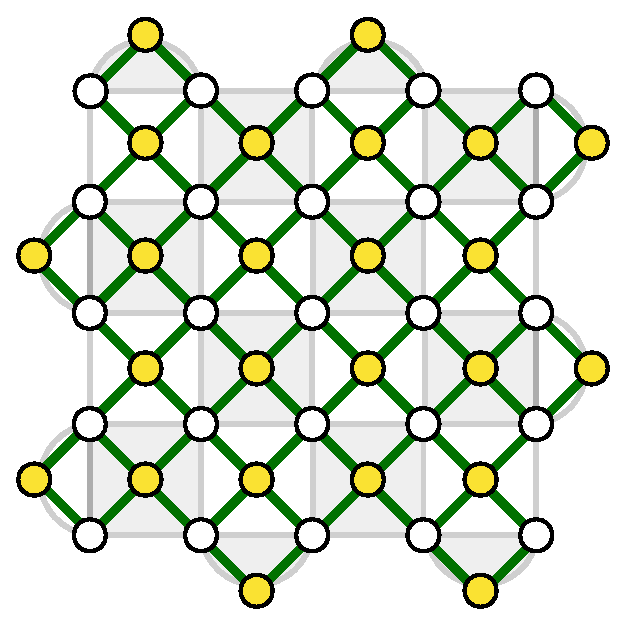
\includegraphics[draft=false,height=0.171\textheight]{figures/fig_surface_layout}\quad\quad\quad
(b)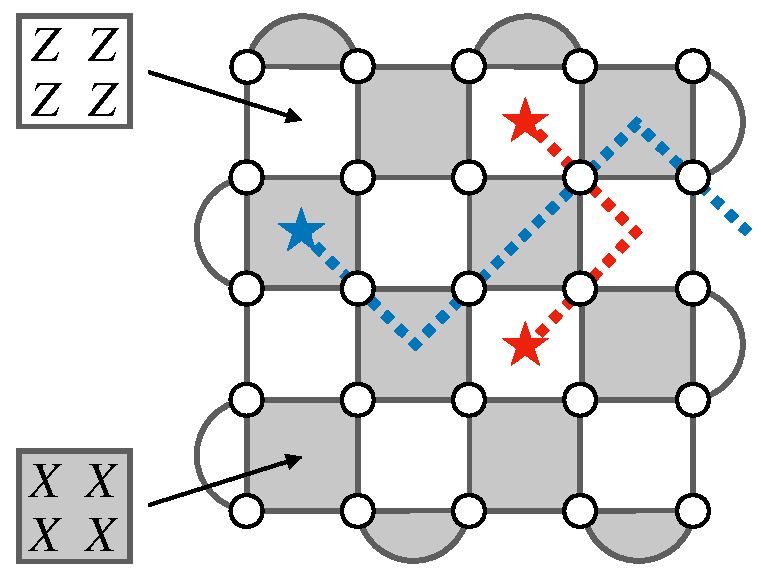
\includegraphics[draft=false,height=0.165\textheight]{figures/fig_surface_error_same}
\caption{
(a) A planar layout of data and ancilla qubits (white and yellow dots, respectively) with entangling gates (green edges) only between neighboring qubits.
This layout gives rise to the $L\times L$ square lattice with open boundary conditions, where $L=5$ here.
(b) The surface code can be realized by measuring Pauli $Z$- and $X$-type parity checks (light and dark faces, respectively). 
The error syndrome (red and blue stars) can be interpreted as the endpoints of string-like Pauli $X$ and $Z$ errors (red and blue dashed edges, respectively).
}
\label{fig:surface_code}
\end{figure}


In order to perform QEC, we have to be able to detect errors without revealing the encoded information.
For stabilizer codes, we can achieve that by measuring their parity checks to obtain the error syndrome (which comprises the measurement outcomes returning $-1$).
Then, the error syndrome is processed by specialized classical algorithms, also known as ``decoders,'' to find an appropriate recovery operator that attempts to remove errors afflicting the encoded information.
For generic stabilizer codes, the problem of optimal decoding is computationally hard, even for simple noise models~\cite{iyer2015hardnessDecoding}.
However, for QEC codes with some underlying structure, such as the surface code, there exist a variety of computationally efficient (albeit not optimal) decoding algorithms.
In particular, the three most popular classes of decoders for the surface code are as follows.
\begin{itemize}
\item Matching decoders, including the minimum-weight perfect matching algorithm~\cite{dennis2002TopologicalQuantumMemory} and its follow-up improvements, such as the belief-matching algorithm~\cite{higgott2023improvedDecodingCircuitNoise}.
These decoders phrase the problem of surface code decoding as a graph-theoretic problem of perfect matching, which can be efficiently solved~\cite{edmonds1965pathsTreesFlowers}.
\item Clustering decoders, such as the renormalization-group decoder~\cite{duclosCianci2010fastDecoders,anwar2014fastDecoders} and the union-find decoder~\cite{delfosse2021almostLinearTimeDecoding}.
These decoders primarily exploit the structure of the error syndrome in the surface code; see Fig.~\ref{fig:surface_code}(b).
\item Tensor-network decoders~\cite{bravyi2014efficientAlgorithmsMaxLikelihood,darmawan2017tensorNetworkSurfaceCode,chubb2021tensorNetworkDecoding}.
These decoders phrase the the problem of surface code decoding as a numerical problem of contracting tensor networks.
\end{itemize}


In order to assess the usefulness of decoders, one usually considers two criteria: runtime and performance.
The first criterion, runtime, is defined as the time needed for the decoder to process the error syndrome.
It is crucial that any practical decoder is able to operate at the rate compatible with the rate of parity check measurements; otherwise, the error syndrome will start to accumulate, leading to the backlog problem~\cite{terhal2015QECforQuantumMemories}.
The second criterion, performance, is typically defined for a given noise model in terms of the logical error rate, i.e., the failure rate of the decoder to successfully undo the effects of noise on the encoded information.
From the perspective of reducing runtime and improving performance, matching and clustering decoders stand out.
Namely, they can achieve almost-linear runtime~\cite{higgott2023sparseBlossom,delfosse2021almostLinearTimeDecoding}, and their performance is close to optimal.
To achieve optimal performance, one can use tensor-network decoders, however they are often not computationally efficient, with runtime that scales unfavorably.


%%%%%%%%%%%%%%%%%%%%%%%%%%%%%%%%%%%%%%%%%%%%%%%%%%%%%%%%%%%%%%%%%%%%%%

\subsubsection*{Rough overview (in math)}


In addition to being compatible with planar layouts of qubits and admitting computationally efficient decoders with good performance, the surface code also exhibits one of the highest QEC thresholds.
Recall that a QEC threshold is specified for the following triple: a QEC code family of growing distance $d$, a decoder and noise model.
It is defined as the highest value $p_\text{th}$ such that for any error rate $p< p_\text{th}$ the probability that the decoder fails to undo the effects of noise goes to zero as $d$ goes to infinity. 
For example, the QEC threshold for the surface code, using minimum-weight perfect matching algorithm, with a circuit noise model based on depolarizing noise, is around $1\%$~\cite{wang2011surfaceCodeErrorRates,higgott2023improvedDecodingCircuitNoise}.


Typically, if the error rate $p$ describing noise is sufficiently low and below the threshold $p_\mathrm{th}$, then the logical error rate $p_\mathrm{fail}$ scales as follows
\begin{equation}
p_\mathrm{fail} \sim \left(\frac{p}{p_\mathrm{th}}\right)^{\left\lceil \frac{d}{2}\right\rceil}.
\end{equation}
This implies that in order to achieve the target error rate $\epsilon$, it suffices to implement the surface code with code distance
$d = \bigO{\log(1/\epsilon) / \log(p_\text{th}/p)}$ using $n + n_A = \bigO{d^2} = \bigO{\log^2(1/\epsilon) / \log^2(p_\text{th}/p)}$ data and ancilla qubits.
Subsequently, qubit overhead associated with QEC based on the surface code only scales polylogarithmically in the inverse target error rate $1/\epsilon$.


%%%%%%%%%%%%%%%%%%%%%%%%%%%%%%%%%%%%%%%%%%%%%%%%%%%%%%%%%%%%%%%%%%%%%%

\subsubsection*{Dominant resource cost (gates/qubits)}


Performing reliable QEC in the presence of measurement errors becomes challenging since the error syndrome can be corrupted.
A straightforward solution to the problem of unreliable error syndrome is to repeatedly measure the parity checks in order to gain enough confidence in their measurement outcomes~\cite{shor1996FTQC,dennis2002TopologicalQuantumMemory}.
If this approach is applied to the surface code with code distance $d$, then one needs to perform $\bigO{d}$ rounds of parity check measurements, incurring relatively large time overhead.


To reduce time overhead, one can pursue single-shot QEC~\cite{bombin2015SingleShotFTQEC}, which does not require repeated measurement rounds.
It is possible to realize single-shot QEC with the surface code~\cite{campbell2019theorySingleShot, ashikhmin2020quantumDataSyndromeCodes, delfosse2022beyondSingleShotFTQC}, however, in addition to parity checks in~\cref{fig:surface_code}(b), one would need to measure nonlocal high-weight parity checks, which is a serious limitation.
A more streamlined approach is to consider a different realization of the surface code, the three-dimensional subsystem toric code~\cite{kubica2022singleShotQECtoric,bridgeman2023liftingTopologicalCodes}, which can be implemented with qubits arranged on the cubic lattice and local low-weight parity checks.
Although this approach is natively defined in three spatial dimensions, it can be emulated with planar layouts of qubits and either a limited number of nonlocal gates or the ability to reshuffle qubits (which is available with, e.g., Rydberg atoms~\cite{saffman2010quantumInfoRydberg,browaeys2020manyBodyRydberg}).
In order to realize code distance $d$ one incurs qubit overhead of $\bigO{d^3}$ (compared to qubit overhead of $\bigO{d^2}$ for the surface code).
From that perspective, single-shot QEC with the subsystem toric code can be viewed as trading time overhead for qubit overhead.


%%%%%%%%%%%%%%%%%%%%%%%%%%%%%%%%%%%%%%%%%%%%%%%%%%%%%%%%%%%%%%%%%%%%%%

\subsubsection*{Caveats}

There have been efforts to improve surface code decoders by incorporating various machine learning methods, including neural networks~\cite{torlai2017neuralDecoder,maskara2019advantagesNeuralNetworkDecoding,chamberland2022techniquesLocalGlobalDecoders} and reinforcement learning~\cite{sweke2021reinforcementLearningDecoders}.
At the current stage, decoders solely based on machine learning methods seem to be of limited applicability, mostly due to high training costs and scalability issues.
Nevertheless, these approaches are likely to be immensely beneficial for QEC in the settings where (possibly correlated) noise is unknown and may have to be learned first. 


Typically, in QEC analysis one considers simple Pauli noise, such as depolarizing noise acting independently and identically on each qubit.
If noise exhibits bias between the $X$, $Y$, and $Z$ components of Pauli noise, then this structure can be exploited, leading to dramatically increased QEC thresholds, as exemplified by variants of the surface code~\cite{tuckett2018ultrahighErrorThreshold,bonillaAtaides2021XZZXsurfaceCode,dua2022cliffordDeformed}.
Similarly, noise that is biased toward erasure errors can be beneficial from the perspective of QEC~\cite{stace2009thresholdsTopologicalCodes,wu2022erasureConversion,kubica2022erasure}.
On the other hand, realistic noise may be coherent or correlated and thus not only difficult to correct, but also to numerically simulate.
For instance, the logical error rates for coherent noise may be orders of magnitude higher than the estimates of the logical error rates for simple Pauli noise (assuming both types of noise have the same error rate)~\cite{iyer2018smallQCneeded}.


In addition to the three-dimensional subsystem toric code, one can also consider other higher-dimensional versions of the surface code.
With these codes, roughly speaking, one improves the QEC capabilities at the expense of increased qubit overhead.
Moreover, for the higher-dimensional surface code, it may suffice to use arguably the least complex decoders that are based on cellular automata (which, by definition, are parallelizable and only use local information about the error syndrome)~\cite{dennis2002TopologicalQuantumMemory,breuckmann2017localDecoders,kubica2019cellularAutomatonDecoders,vasmer2021cellularAtomatonDecoders}.


%%%%%%%%%%%%%%%%%%%%%%%%%%%%%%%%%%%%%%%%%%%%%%%%%%%%%%%%%%%%%%%%%%%%%%

\subsubsection*{Example use cases}


\begin{itemize}
    \item Decoders for the surface code can be used for other QEC code families, such as the color code~\cite{bombin2006topologicalQuantumDistillation,bombin2007exactTopologicalQuantumOrder,kubica2018phdThesis}.
    In fact, due to a close connection between the color codes and the surface codes~\cite{bombin2012universalTopologicalPhase,kubica2015unfoldingColorCode}, any surface code decoder can be used as a subroutine in the restriction decoder for any color code (in two or more spatial dimensions)~\cite{kubica2023efficientColorCodeDecoders,vasmer2022morphingQuantumCodes}. 
\end{itemize}

%%%%%%%%%%%%%%%%%%%%%%%%%%%%%%%%%%%%%%%%%%%%%%%%%%%%%%%%%%%%%%%%%%%%%%

\subsubsection*{Further reading}

\begin{itemize}
    \item The seminal paper by Dennis et al.~\cite{dennis2002TopologicalQuantumMemory} is a thorough introduction to QEC with the surface code.
    \item A recent perspective \cite{brown2023conservationLawsQEC} on how to use matching decoders to decode stabilizer codes.
    \item Open-source software packages have been developed for implementing QEC with the surface code, such as Stim~\cite{gidney2021Stim} and PyMatching~\cite{higgott2021PyMatching}.
\end{itemize}

%%%%%%%%%%%%%%%%%%%%%%%%%%%%%%%%%%%%%%%%%%%%%%%%%%%%%%%%%%%%%%%%%%%%%%
\printbibliography[heading=secbib,segment=\therefsegment]

\end{refsection}
 

\newpage 

%%%%%%%%%%%%%%%%%%%%%%%%%%%%%%%%%%%%%%%%%
%%%%%%%%%%%%%%%%%%%%%%%%%%%%%%%%%%%%%%%%%


\begin{refsection}
\section{Logical gates with the surface code}
\label{prim:LatticeSurgery}

%%%%%%%%%%%%%%%%%%%%%%%%%%%%%%%%%%%%%%%%%%%%%%%%%%%%%%%%%%%%%%%%%%%%%%

\subsubsection*{Rough overview (in words)}


The ability to implement an arbitrary unitary operation, either exactly or approximately, is a prerequisite for performing quantum computation.
It can be achieved with unitary gates that form a universal gate set~\cite{kitaev1997quantumComputationsAlgosQEC,nielsen2002QCQI}.
A commonly considered gate set contains two Clifford gates, the Hadamard gate $H$ and the controlled-$X$ gate $CX$ (also known as the controlled NOT gate), and one non-Clifford gate, the $T = Z^{1/4}$ gate.
One can consider other non-Clifford gates, such as the Toffoli gate $CCX$.
Note that non-Clifford gates are essential for quantum computation, as any quantum circuit comprising only Clifford gates, state preparation, and measurement in the computational basis can be simulated in polynomial time on a probabilistic classical computer~\cite{gottesman1998HeisenbergRepresentation,aaronson2004improvedSimulationStabilizer}.


Since we are interested in fault-tolerant quantum computation, we would like to implement a universal set of logical gates $\overline H$, $\overline{CX}$, and $\overline T$ on information encoded in some QEC code, such as \hyperref[prim:QEC]{the surface code}.
We can implement these gates with a planar layout of qubits and nearest-neighbor entangling gates.
To be more precise, we consider a simple architecture~\cite{horsman2012latticeSurgery} that comprises $N$ surface code patches, each encoding a logical qubit into the surface code with code distance $d$, and the routing space in between; see~\cref{fig:planar}(a).
In such an architecture, the total number of data and ancilla qubits is $\mathcal O(N d^2)$.


\begin{figure}[h]
\centering
(a)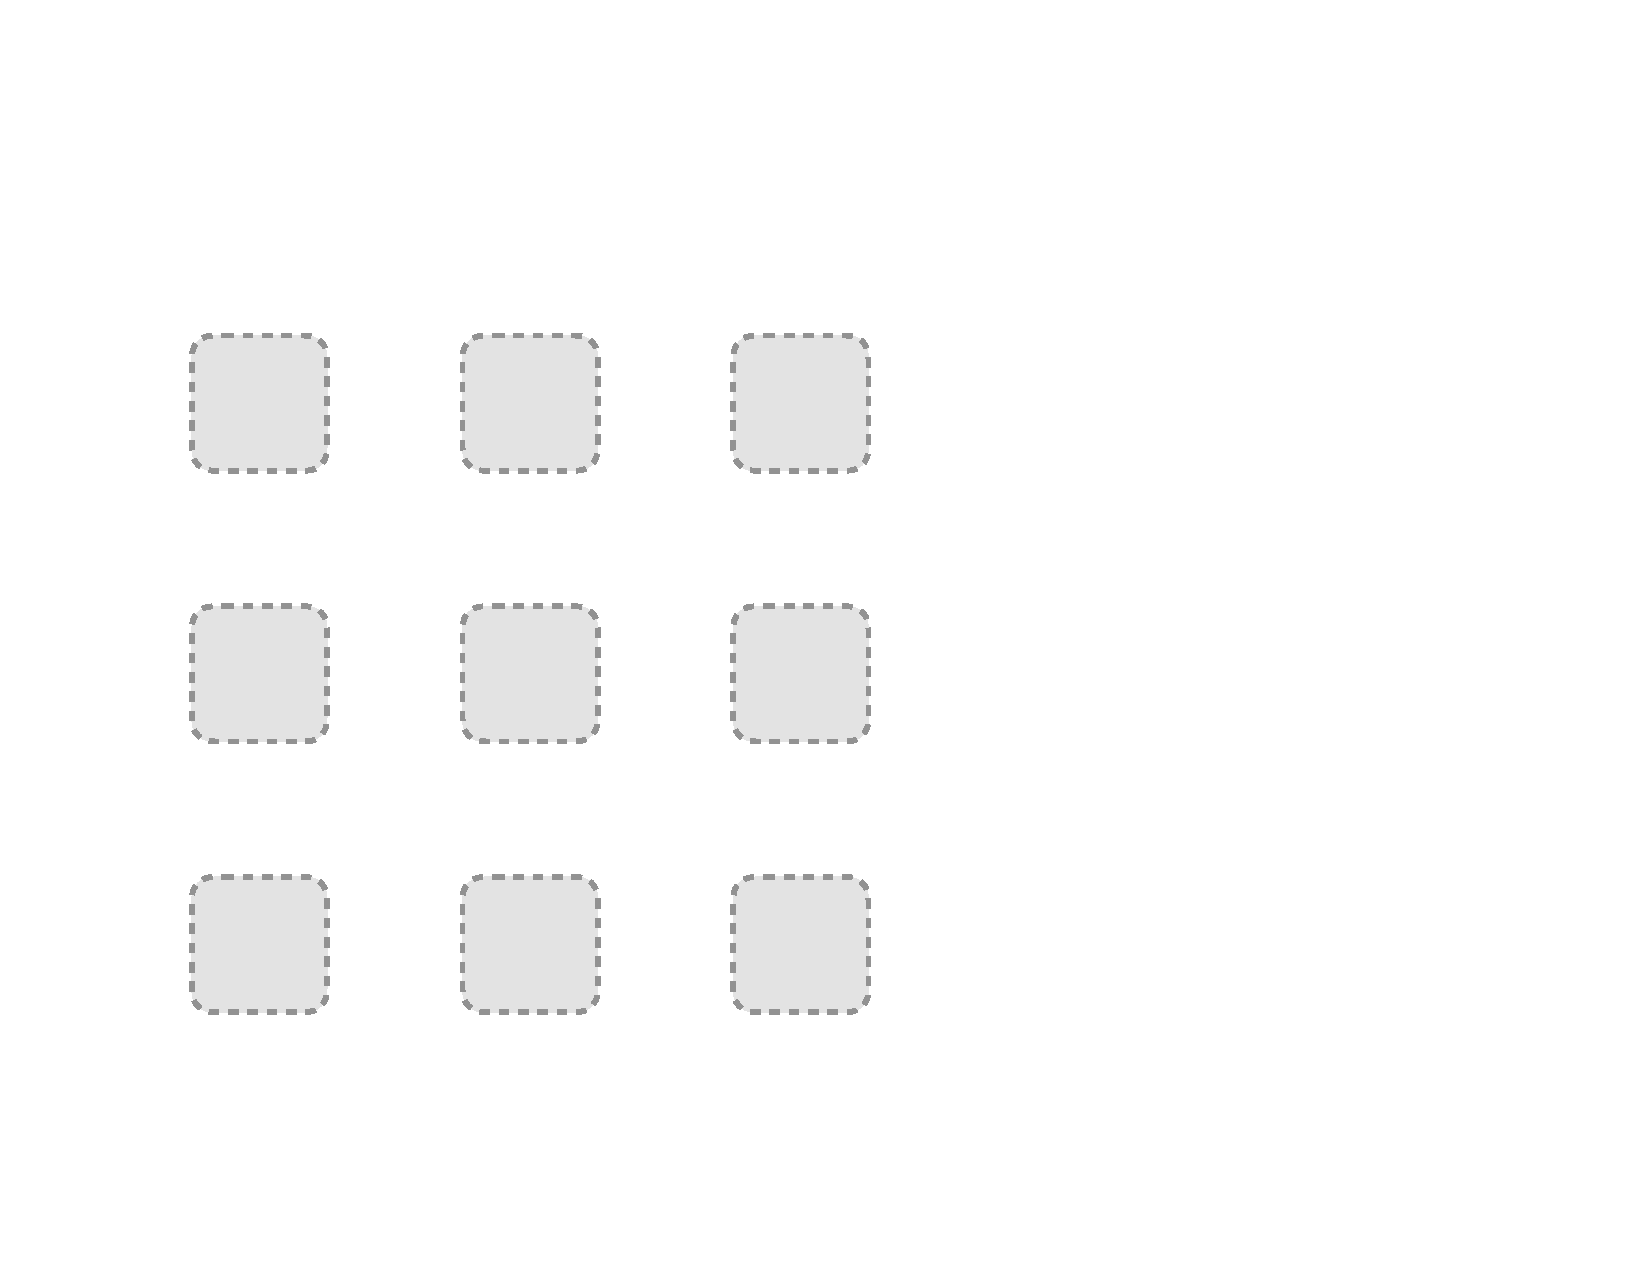
\includegraphics[draft=false,height=0.17\textheight]{figures/fig_planar}\quad\quad\quad
(b)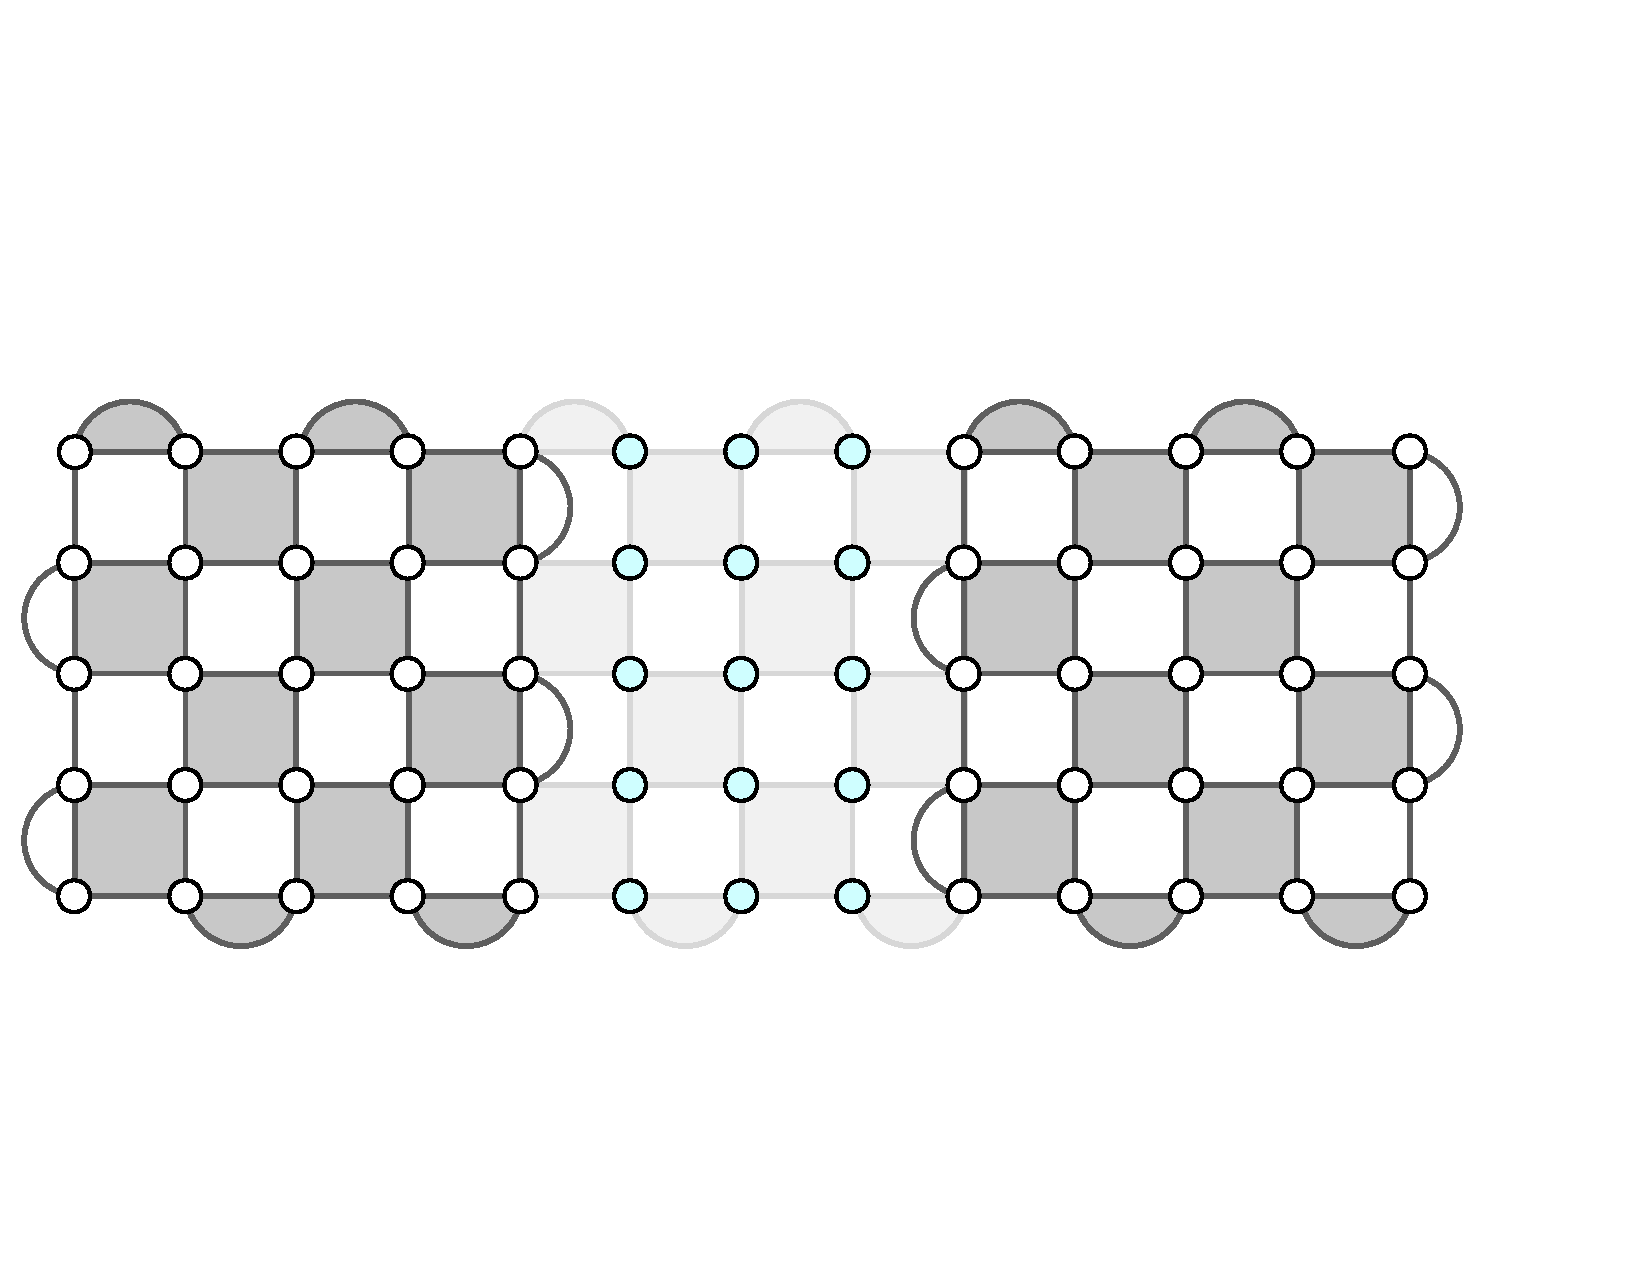
\includegraphics[draft=false,height=0.17\textheight]{figures/fig_surgery}
\caption{
(a) A planar layout of qubits comprises surface code patches (shaded), each using the layout depicted in~\cref{fig:surface_code}(a) and encoding a logical qubit, and the routing space in between. 
(b) Logical Pauli measurement $\overline{M_{XX}}$ is implemented by preparing the routing space qubits (turquoise dots) in the state $\ket 0$ and repeatedly measuring parity checks (lightly shaded) in the routing space spanning between the two surface code patches.
Other logical Pauli measurements, e.g., $\overline{M_{ZZ}}$ and $\overline{M_{YZ}}$, require connecting different boundaries of the two patches.
}
\label{fig:planar}
\end{figure}


%%%%%%%%%%%%%%%%%%%%%%%%%%%%%%%%%%%%%%%%%%%%%%%%%%%%%%%%%%%%%%%%%%%%%%

\subsubsection*{Rough overview (in math)}


The logical $\overline H$ does not pose any challenges.
From a practical standpoint, it is transversal, since it can be realized by applying the Hadamard gate $H$ to every data qubit in the surface code patch, followed by swapping of the roles of Pauli $Z$- and $X$-type parity checks in the subsequent QEC rounds.
As such, the logical $\overline H$ takes constant time and the surface code patch is effectively rotated (which may alter how subsequent operations are implemented).


The logical $\overline{CX}$ is more challenging than the logical $\overline H$, since it is impossible to implement it transversally with the planar layout of qubits and nearest-neighbor entangling gates shown in~\cref{fig:planar}(a).
Instead, one can use the following quantum circuit, where the first qubit (top wire) is the control and the third qubit (bottom wire) is the target of the logical $\overline{CX}$ gate
\begin{equation}
\begin{split}
\Qcircuit @C=.7em @R=.3em {
	& \ustick{a} \cwx[1]		& 					& 				&		\\	
	& \multigate{1}{\overline{M_{ZZ}}} 	& \qw 				& \gate{\overline{Z}^{\, b}}		& \qw		\\
\lstick{\ket{\overline{+}}}& \ghost{M_{ZZ}} 		& \multigate{1}{\overline{M_{XX}}} 	& \gate{\overline{M_Z}}		& \rstick{c}\cw	\\
	& \qw 				& \ghost{M_{XX}} 		& \gate{\overline{X}^{\, a+c}}	& \qw 		\\
	& 					& \dstick{b} \cwx[-1]		& 				&
}\\
\ 
\end{split}
\end{equation}
It is straightforward to fault-tolerantly realize preparation of the logical state $\ket{\overline{+}}$, logical Pauli measurement $\overline{M_Z}$, and logical Pauli operators $\overline{Z}$ and $\overline{X}$.
In addition, the required logical Pauli measurements $\overline{M_{ZZ}}$ and $\overline{M_{XX}}$ can be implemented fault-tolerantly via ``lattice surgery'' techniques~\cite{horsman2012latticeSurgery}; see~\cref{fig:planar}(b) for an illustration of how to realize $\overline{M_{XX}}$.
Unlike the logical $\overline H$, logical Pauli measurements $\overline{M_{ZZ}}$ and $\overline{M_{XX}}$ and, subsequently, the logical $\overline{CX}$ cannot be realized in constant time; rather, due to the need to account for measurement errors, they typically incur time overhead of $\bigO{d}$.


The logical $\overline T$ can be implemented using gate teleportation~\cite{gottesman1999viabilityUniversalQC} via the following quantum circuit
\begin{equation}
\begin{split}
\Qcircuit @C=.7em @R=.3em {
					& \multigate{1}{\overline{CX}}	& \gate{\overline{S}^{\, a}} & \qw		\\
\lstick{\ket{\overline{T}}} 	& \ghost{\overline{CX}}		& \gate{\overline{M_Z}}	& \rstick{a} \cw 
}
\end{split}
\label{eq:gate_teleportation}
\end{equation}
where the logical resource state $\ket{\overline{T}} = \left(\ket{\overline{0}} + e^{i\pi/4}\ket{\overline{1}}\right)/\sqrt{2}$, the logical gate $\overline{S} = \overline{Z}^{\,1/2}$, and the first qubit (top wire) is the control and the second qubit (bottom wire) is the target of the logical $\overline{CX}$ gate.
Even though the logical $\overline{S}$ is a Clifford gate, its fault-tolerant implementation with the surface code may not be effortless~\cite{brown2017pokingHoles} (unless one uses nonlocal entangling gates~\cite{kubica2015unfoldingColorCode,moussa2016transversalCliffordGates})
Moreover, the need to apply the logical $\overline{S}$ conditioned on the measurement outcome of $\overline{M_Z}$ may slow down quantum computation.
For that reason, it may be beneficial to use the following quantum circuit from \cite[Fig.~17(b)]{litinski2019gameofsurfacecodes}
\begin{equation}
\begin{split}
\Qcircuit @C=.7em @R=.3em {
			& \ustick{a} \cwx[1]		& 							& 					&			\\	
\lstick{\ket{\overline{0}}}& \multigate{1}{\overline{M_{YZ}}} 	& \gate{\overline{H}^{\, b}}	& \gate{\overline{M_Z}}	& \rstick{c}\cw	\\
\lstick{\ket{\overline{T}}}& \ghost{M_{YZ}} 		& \multigate{1}{\overline{M_{ZZ}}} 	& \gate{\overline{M_X}}	& \rstick{d}\cw	\\
			& \qw 				& \ghost{M_{ZZ}} 				& \gate{\overline{Z}^{\, ab+c+d}}& \qw 		\\
			& 					& \dstick{b} \cwx[-1]				& 					&
}\\
\ 
\end{split}
\label{eq:autocorrected}
\end{equation}
which is an alternative to the one in~\cref{eq:gate_teleportation} that uses one additional logical qubit but requires only logical Pauli corrections, rather than logical Clifford corrections.
In either case, given the logical resource state $\ket{\overline T}$, the logical $\overline T$ typically incurs time overhead of $\bigO{d}$.
We conclude that implementing the logical $\overline T$ reduces to the problem of preparing the logical state $\ket{\overline{T}}$, which, in turn, can be realized via state distillation~\cite{knill2004FTPostSelectedQC,bravyi2005UniversalQC}; see  \cite{beverland2021costUniversality} for a brief overview of state distillation.


%%%%%%%%%%%%%%%%%%%%%%%%%%%%%%%%%%%%%%%%%%%%%%%%%%%%%%%%%%%%%%%%%%%%%%

\subsubsection*{Dominant resource cost (gates/qubits)}


State distillation provides a fault-tolerant method to prepare high-fidelity logical resource states, such as the logical state $\ket{\overline T}$.
The basic idea is to convert some number of noisy resource states into fewer but, crucially, less noisy resource states.
Importantly, this task can be accomplished with quantum circuits comprising only Clifford gates (together with state preparation and measurement in the computational basis) and postselection.
Typically, state distillation circuits are based on some QEC code, e.g., the 15-qubit Reed--Muller code.

State distillation is often described as a resource-intensive method that contributes the most to the resource overhead of fault-tolerant quantum computation with the surface code~\cite{fowler2012SurfaceCodes} and, for that reason, many efforts have been devoted to finding possible alternatives~\cite{bravyi2015doubledColorCodes,jochymOConnor2016stackedCodes,bombin20182DquantumComputation,chamberland2019faultTolerantMagicStateFlagQubits,beverland2021costUniversality}. 
However, recent results indicate that state distillation may not be as costly as one may think~\cite{litinski2019gameofsurfacecodes,litinski2019magicstate}, especially when one optimizes it for specific quantum hardware and noise that exhibits some bias~\cite{litinski2022activeVolume}.
In the task of estimating the ground state energy density of the \hyperref[appl:FermiHubbard]{Fermi--Hubbard model}, state distillation of logical Toffoli resource states injected one at a time uses less than $10\%$ of the total resources and is never a bottleneck on runtime of the quantum algorithm~\cite{chamberland2022buildingFTQC}.


Oftentimes, a quantum algorithm is expressed as a quantum circuit $\mathcal C$ comprising Clifford and $T$ gates.
Thus, by using the aforementioned logical gates $\overline H$, $\overline{CX}$, and $\overline{T}$, we can fault-tolerantly implement the logical quantum circuit $\overline{\mathcal C}$ with the surface code of code distance $d$ and a planar layout of qubits in~\cref{fig:planar}(a).
However, from the perspective of reducing the resource overheads, it may be beneficial  to consider a quantum circuit $\mathcal C'$ equivalent to the circuit $\mathcal C$, which is obtained from $\mathcal C$ by commuting all Clifford gates to the end of $\mathcal C$~\cite{litinski2019gameofsurfacecodes}.
As a result, the circuit $\mathcal C'$ only comprises multiqubit Pauli $\pi/8$ rotations (which are a generalization of the $T$ gate and can be realized via, e.g., quantum circuits analogous to the one in~\cref{eq:autocorrected}).
Consequently, fault-tolerant implementation of the logical circuit $\overline{\mathcal{C}'}$ incurs the qubit overhead of $\bigO{Nd^2}$ and time overhead of $\bigO{Md}$, where $N$ and $M$ are the number of, respectively, qubits and $T$ gates in $\mathcal C$.
We remark that the time overhead can be reduced at the expense of increased qubit overhead---first by distilling more resource states and being able to use them faster, then by implementing them in parallel~\cite{litinski2019gameofsurfacecodes}.


%%%%%%%%%%%%%%%%%%%%%%%%%%%%%%%%%%%%%%%%%%%%%%%%%%%%%%%%%%%%%%%%%%%%%%

\subsubsection*{Caveats}


Lattice surgery is not necessary to realize fault-tolerant quantum computation with a planar layout of qubits and nearest-neighbor gates.
An alternative approach (which actually preceded the development of lattice surgery) relies on the surface code with defects and braiding~\cite{raussendorf2007FTQChighThreshold,raussendorf2007topologicalFaultTolerance,fowler2012SurfaceCodes,brown2017pokingHoles}.
However, resource overhead estimates strongly suggest that this approach is not competitive with lattice surgery~\cite{fowler2018}.


A simple architecture depicted in~\cref{fig:planar}(a) can be improved in a couple ways to reduce the qubit overhead.
First, it is possible to pack surface code patches more densely, resulting in more logical qubits for the given total number of qubits and target code distance~\cite{lao2018mappingLatticeSurgery,litinski2019gameofsurfacecodes}
Second, one can designate certain regions, commonly referred to as magic state factories, to solely produce resource states, such as the logical state $\ket{\overline T}$, and optimize their design~\cite{OGorman2017magicStateFactories,litinski2019gameofsurfacecodes,litinski2019magicstate}.


To simplify implementation of logical gates, one can consider other QEC codes, e.g., the three-dimensional color code~\cite{bombin2015gaugeColorCodes,kubica2015universalTransversalGates}.
The gauge color code has redundant degrees of freedom, commonly referred to as gauge qubits. 
For different states of its gauge qubits, the gauge color code admits transversal implementation of different logical gates, which, \emph{combined}, form a universal gate set (thus circumventing the Eastin--Knill theorem~\cite{eastin2009RestrictionsTransversal,zeng2011Transversality}).
Importantly, changing the state of gauge qubits can be done fault-tolerantly in constant time.
However, to realize this construction one needs, for instance, a three-dimensional layout of qubits with nearest-neighbor gates or a planar layout of qubits with a limited number of nonlocal gates, which are more challenging to engineer compared to the simple architecture in~\cref{fig:planar}(a).
To achieve code distance $d$ with the gauge color code one incurs qubit overhead of $\bigO{d^3}$ (compared to qubit overhead of $\bigO{d^2}$ for the surface code), so, similarly to single-shot QEC described in~\cref{prim:QEC}, this approach trades time overhead for qubit overhead. 


%%%%%%%%%%%%%%%%%%%%%%%%%%%%%%%%%%%%%%%%%%%%%%%%%%%%%%%%%%%%%%%%%%%%%%

\subsubsection*{Example use cases}


\begin{itemize}
\item Lattice surgery techniques developed for the surface code can be straightforwardly adapted to, e.g., the color code~\cite{landahl2014colorCodeLatticeSurgery} or the surface code with a twist~\cite{yoder2017surfaceCodeTwist}, leading to fault-tolerant quantum computation with potentially reduced qubit overhead.
In addition, lattice surgery techniques can also be used for the fault-tolerant transfer of encoded information between arbitrary topological quantum codes~\cite{poulsenNautrup2017faultTolerantInterface}.
\item 
Now, we are ready to present a rough, order-of-magnitude estimate of the resource overheads needed to realize fault-tolerant quantum computation in the architecture based on the surface code and lattice surgery.
For concreteness, we consider the circuit noise of strength $p=0.001$, where each basic operation, including state preparation, CNOT gate, and measurement, can fail with probability $p$.
Assume that we want to implement a quantum circuit $\mathcal C$ comprising $N=10^3$ qubits and a certain number $M=10^{10}$ of $T$ gates. These resource counts are in the ballpark of estimates for various quantum algorithms in the application areas of \hyperref[appl:QuantumChemistry]{quantum chemistry}, hyperref[appl:CondensedMatter]{condensed matter physics}, and \hyperref[appl:cryptanalysis]{cryptanalysis}.
First, following the procedure from~\cite{litinski2019gameofsurfacecodes}, we compile $\mathcal C$ into a new circuit $\mathcal C'$ of depth $M$ that comprises $N$ qubits and $M$ multiqubit Pauli $\pi/8$-rotations implemented one at a time.
Since there are $NM$ possible fault locations in the circuit $\mathcal C'$, the error rate for each qubit of $\mathcal C'$ should not exceed than
\begin{equation}
\epsilon \approx 1/(N M).
\end{equation}
Since each qubit of $\mathcal C'$ is realized as a logical qubit of the surface code with distance $d$, then its
logical error rate $p_\text{fail}$ can be approximated by 
\begin{equation}
p_\text{fail} \approx \alpha (p/p_\text{th})^{d/2},
\end{equation}
where we can crudely set $\alpha = 0.05$ and $p_\text{th} = 0.01$; see \hyperref[prim:QEC]{quantum error correction with the surface code} for more details.
Note that these values are empirical and depend heavily on the choice of the decoder; in our case---the belief-matching algorithm~\cite{higgott2023improvedDecodingCircuitNoise}.
Thus, in order for the logical error rate $p_\text{fail}$ to reach the target error rate $\epsilon$ we need the surface code distance at least
\begin{equation}
d \approx \left\lceil 2 \log(\alpha N M)/\log(p_\mathrm{th}/p) \right\rceil.
\end{equation}
Assuming that half of all required qubits is devoted to realizing $N$ surface code patches (each comprising $2d^2-1$ data and ancilla qubits), with the other half used for resource state distillation and routing,
we obtain that the fault-tolerant implementation of $\mathcal C'$ incurs qubit overhead of
\begin{equation}
n_{\mathcal C'} \approx 4Nd^2
\end{equation}
and time overhead of
\begin{equation}
t_{\mathcal C'} \approx Md\tau,
\end{equation}
where we crudely set $\tau = 1\ \!\mu s$ to be the time needed to implement one syndrome measurement round with the superconducting circuits architecture.
Finally, our order-of-magnitude resource estimate gives $2.3\times 10^6$ physical qubits and $67$ hours of runtime.
This general approach to resource estimation has been applied to a number of specific quantum algorithms in a variety of \hyperref[applications]{application areas}; see, e.g.,~\cite{lee2021EvenMoreEfficientChemistryTensorHyp, gidney2021HowToFactor, Kivlichan2020ImprovedFaultTolerantSimulationCondensedMatter,Beverland2022Requirements,sanders2020FTQCforCombOpt}. These references often go beyond a back-of-the-envelope calculation and provide a more meticulous analysis that accounts for exact qubit layouts and the physical footprint of resource state distillation factories. They also pursue optimizations to how the circuit is implemented (e.g.~exploiting space-time tradeoffs) in light of these considerations. 

\end{itemize}



%%%%%%%%%%%%%%%%%%%%%%%%%%%%%%%%%%%%%%%%%%%%%%%%%%%%%%%%%%%%%%%%%%%%%%

\subsubsection*{Further reading}

\begin{itemize}
\item An accessible overview of fault-tolerant quantum computation based on the surface code and lattice surgery can be found in  \cite{litinski2019gameofsurfacecodes}. 
\item A convenient way to describe and optimize lattice surgery operations is via the ZX calculus, which is a diagrammatic language for quantum computing~\cite{coecke2017picturingQuantumProcesses,deBeaudrap2020ZXcalculusLatticeSurgery}.
\item A direct comparison of the resource overhead associated with preparation of the logical resource state $\ket{\overline T}$ using either state distillation or transversal gates (with the three-dimensional color code) can be found in  \cite{beverland2021costUniversality}.
\item To read about a framework for estimating resources required to realize large-scale fault-tolerant quantum computation, see  \cite{Beverland2022Requirements}.
\end{itemize}

%%%%%%%%%%%%%%%%%%%%%%%%%%%%%%%%%%%%%%%%%%%%%%%%%%%%%%%%%%%%%%%%%%%%%%
\printbibliography[heading=secbib,segment=\therefsegment]

\end{refsection}

%%%%%%%%%%%%%%%%%%%%%%%%%%%%%%%%%%%%%%%%%%%%%%%%%%%%%%%%%%%%%%%%%%%%%%
% \ifdraft{
% \appendix
% \chapter{Conventions}
% \section{Some wording conventions}

\begin{itemize}
    \item We opt for American conventions over British (optimization, not optmisation, flavor, not flavour, etc.)
    \item Conventions on specific words with multiple spellings: parametrized (not parameterized)
    \item Words like nontrivial and nonsingular should not be hyphenated, unless it would be confusing otherwise (e.g.~a double consonant, so non-negative is ok). Some specific words that we are always hyphenating / not hyphenating:
    \begin{itemize}
        \item No hyphens: postselection, nonzero, nonlinear, nondestructive, speedup, nonuniform, subquadratic, nonparametric, suboptimal, subnormalization, tradeoff
        \item Hyphens: non-unitary, non-square, block-encoding
    \end{itemize}
    \item Only first word of Title (of section, subsection, etc) is capitalized, except for proper nouns or words following colons. 
    \item Monte Carlo has no hyphen, but capitalized. This includes ``Monte Carlo--style algorithms" which technicallyuses an ``en dash'' between ``Monte Carlo'' and ``style'' (rather than a hyphen)
    \item Use ``analog" for e.g. ``analog quantum simulator". Use ``analogue" for other cases, e.g. ``X is an analogue of Y". See discussion here: \url{https://grammarist.com/spelling/analog-analogue/}
    \item Use ``nature" over ``Nature"
    \item $T$ gate (no hyphen, math mode for $T$), but $T$-count, and $T$-depth (with hyphen)
    \item We include the Oxford comma on a list of 3 or more items, e.g., ``we often want to form a single block-encoding of a product, tensor product, or linear combination of the individual block-encoded operators.''
\end{itemize}

\section{Typesetting conventions}

\begin{itemize}
    \item Following American (over British) conventions, put punctuation such as commas and periods inside of the end quotation, and use ``double quotations.'' The only isntance where `single quotations' would be used is for nested quotations. 
    \item Footnotemarks should appear after periods and commas, but inside quotation marks
\end{itemize}

\section{Matrices, vectors, dot products}
\begin{itemize}
    \item Vectors should appear in lowercase latin letters
    \item The all-ones vector should appear as $\mathbf{1}$.
    \item Matrices should appear in uppercase latin letters
    \item Dot products between vectors $u$ and $v$ can be denoted either by $u^\intercal v$ or by $\langle u, v \rangle$, but the definition of $\langle \cdot, \cdot \rangle$ should be restated the first time it appears in each article
\end{itemize}

\section{QRAM vs.~QROM}
Most often, we refer to a classical-write quantum-read version of QRAM, which we can just call QRAM, but if there might be confusion, the ``classical-write quantum-read'' qualifier can be added the first time it appears in an article. 


\section{Big-$\mathcal{O}$ notation}\label{app:bigO}
We are using $\mathcal{O}$ for big-O notation, and $\tilde{\mathcal{O}}$ when logarithmic factors are suppressed. The meaning of the tilde should ideally be restated in each article when it first appears. You can use the command \textbackslash{bigO} and \textbackslash{bigOt} commands which have been defined in the preamble. 

\section{In-text citations}

When citing something, no need to spell out ``Ref.'' Just cite directly as [4] or [5], e.g.~``As shown in [5], ...''
% }
% {}

\endgroup  % End group where backref is turned off (i.e. backref is now back on)


%% Consolidated bibliography with backrefs
\begingroup
\newpage
\pagestyle{chapterpage}
\nocite{*}
\printbibliography[env=globalbibliography, title={Consolidated bibliography}, category=cited, heading=bibintoc]\label{ch:globalbib}
\endgroup


\end{document}
